% =====================================================================
%  Tesi di laurea — file principale
%
%  Compilare con pdfLaTeX DUE VOLTE: la prima passata scrive main.aux,
%  la seconda risolve riferimenti incrociati e indice.
%      pdflatex main.tex && pdflatex main.tex
% =====================================================================
\documentclass[12pt,a4paper,oneside]{report}

\usepackage[utf8]{inputenc}
% T2A copre l'alfabeto cirillico, T1 resta la codifica predefinita per il testo.
\usepackage[T2A,T1]{fontenc}
\usepackage[italian]{babel}
\usepackage{lmodern}
% Permette di comporre lettere greche in modo diretto nel testo.
\usepackage{textalpha}

\usepackage{amsmath,amssymb}
\usepackage{array}
\usepackage{booktabs}
\usepackage{graphicx}
\usepackage{siunitx}
\usepackage[margin=3cm]{geometry}
\usepackage{caption}
\usepackage[hidelinks]{hyperref}
% Consente agli indirizzi lunghi di andare a capo (Appendice B).
\usepackage{xurl}

\sisetup{group-separator={\,},group-minimum-digits=4}
\captionsetup{font=small,labelfont=bf}

% Margine di elasticità per le righe difficili da giustificare.
\emergencystretch=1em

% Collocazione delle figure. I valori predefiniti di LaTeX sono prudenti e
% mandano in pagina separata ogni figura che superi il 70%% dell'altezza,
% lasciando pagine di sole immagini. Qui si consente a una figura di
% condividere la pagina con poco testo, e a più figure di stare insieme.
\renewcommand{\topfraction}{0.9}
\renewcommand{\bottomfraction}{0.7}
\renewcommand{\textfraction}{0.07}
\renewcommand{\floatpagefraction}{0.8}
\setcounter{topnumber}{4}
\setcounter{bottomnumber}{2}
\setcounter{totalnumber}{6}

% Compone testo che mescola alfabeti diversi. Commuta alla codifica T2A, che
% contiene sia le lettere latine sia quelle cirilliche; il greco resta gestito
% da textalpha, che seleziona da sé la codifica LGR.
\newcommand{\multiscritto}[1]{{\fontencoding{T2A}\selectfont #1}}

\begin{document}

% =====================================================================
%  FRONTESPIZIO
% =====================================================================
% =====================================================================
%  Frontespizio ufficiale del Dipartimento di Fisica e Astronomia
%  Adattato dal modello frontespizio-fisica.tex.
%  Incluso da main.tex con % =====================================================================
%  Frontespizio ufficiale del Dipartimento di Fisica e Astronomia
%  Adattato dal modello frontespizio-fisica.tex.
%  Incluso da main.tex con % =====================================================================
%  Frontespizio ufficiale del Dipartimento di Fisica e Astronomia
%  Adattato dal modello frontespizio-fisica.tex.
%  Incluso da main.tex con \input{frontespizio}
%
%  Il modello impone \textwidth = 450pt e \oddsidemargin = 0pt: qui la
%  misura viene applicata con \newgeometry alla SOLA pagina del titolo e
%  revocata subito dopo con \restoregeometry, così che il resto della tesi
%  conservi i margini di 3 cm dichiarati nel preambolo.
%
%  I comandi \textcolor{red}{...} del modello servivano solo a evidenziare
%  i campi da compilare; una volta compilati equivalgono a testo nero e
%  sono stati rimossi, come prescrive il commento del modello stesso.
%
%  Rispetto al modello è stato eliminato il blocco del correlatore, che
%  non è previsto in questo lavoro.
% =====================================================================

\newgeometry{left=2.54cm, right=2.63cm, top=4.6cm, bottom=2cm}

\begin{titlepage}

\begin{center}
{{\Large{\textsc{Alma Mater Studiorum $\cdot$ Universit\`a di Bologna}}}}
\rule[0.1cm]{15.8cm}{0.1mm}
\rule[0.5cm]{15.8cm}{0.6mm}
\\\vspace{3mm}

{\small{\bf Dipartimento di Fisica e Astronomia ``Augusto Righi''\\
Corso di Laurea in Fisica}}

\end{center}

\vspace{23mm}

\begin{center}
%
% TITOLO DELLA TESI
%
{\LARGE{\bf Fra ordine e disordine}}\\[5mm]
{\Large{\bf Propriet\`a statistiche del linguaggio\\
generato da Large Language Model}}
\end{center}

\vspace{50mm} \par \noindent

\begin{minipage}[t]{0.47\textwidth}
%
% RELATORE
%
{\large{\bf Relatore: \vspace{2mm}\\
Prof. Mirko Degli Esposti}}
\end{minipage}
%
\hfill
%
\begin{minipage}[t]{0.47\textwidth}\raggedleft
{\large{\bf Presentata da:
\vspace{2mm}\\
%
% CANDIDATO
%
Samuele Zurlo}}
\end{minipage}

\vspace{40mm}

\begin{center}
%
% ANNO ACCADEMICO
%
Anno Accademico 2025/2026
\end{center}

\end{titlepage}

\restoregeometry

%
%  Il modello impone \textwidth = 450pt e \oddsidemargin = 0pt: qui la
%  misura viene applicata con \newgeometry alla SOLA pagina del titolo e
%  revocata subito dopo con \restoregeometry, così che il resto della tesi
%  conservi i margini di 3 cm dichiarati nel preambolo.
%
%  I comandi \textcolor{red}{...} del modello servivano solo a evidenziare
%  i campi da compilare; una volta compilati equivalgono a testo nero e
%  sono stati rimossi, come prescrive il commento del modello stesso.
%
%  Rispetto al modello è stato eliminato il blocco del correlatore, che
%  non è previsto in questo lavoro.
% =====================================================================

\newgeometry{left=2.54cm, right=2.63cm, top=4.6cm, bottom=2cm}

\begin{titlepage}

\begin{center}
{{\Large{\textsc{Alma Mater Studiorum $\cdot$ Universit\`a di Bologna}}}}
\rule[0.1cm]{15.8cm}{0.1mm}
\rule[0.5cm]{15.8cm}{0.6mm}
\\\vspace{3mm}

{\small{\bf Dipartimento di Fisica e Astronomia ``Augusto Righi''\\
Corso di Laurea in Fisica}}

\end{center}

\vspace{23mm}

\begin{center}
%
% TITOLO DELLA TESI
%
{\LARGE{\bf Fra ordine e disordine}}\\[5mm]
{\Large{\bf Propriet\`a statistiche del linguaggio\\
generato da Large Language Model}}
\end{center}

\vspace{50mm} \par \noindent

\begin{minipage}[t]{0.47\textwidth}
%
% RELATORE
%
{\large{\bf Relatore: \vspace{2mm}\\
Prof. Mirko Degli Esposti}}
\end{minipage}
%
\hfill
%
\begin{minipage}[t]{0.47\textwidth}\raggedleft
{\large{\bf Presentata da:
\vspace{2mm}\\
%
% CANDIDATO
%
Samuele Zurlo}}
\end{minipage}

\vspace{40mm}

\begin{center}
%
% ANNO ACCADEMICO
%
Anno Accademico 2025/2026
\end{center}

\end{titlepage}

\restoregeometry

%
%  Il modello impone \textwidth = 450pt e \oddsidemargin = 0pt: qui la
%  misura viene applicata con \newgeometry alla SOLA pagina del titolo e
%  revocata subito dopo con \restoregeometry, così che il resto della tesi
%  conservi i margini di 3 cm dichiarati nel preambolo.
%
%  I comandi \textcolor{red}{...} del modello servivano solo a evidenziare
%  i campi da compilare; una volta compilati equivalgono a testo nero e
%  sono stati rimossi, come prescrive il commento del modello stesso.
%
%  Rispetto al modello è stato eliminato il blocco del correlatore, che
%  non è previsto in questo lavoro.
% =====================================================================

\newgeometry{left=2.54cm, right=2.63cm, top=4.6cm, bottom=2cm}

\begin{titlepage}

\begin{center}
{{\Large{\textsc{Alma Mater Studiorum $\cdot$ Universit\`a di Bologna}}}}
\rule[0.1cm]{15.8cm}{0.1mm}
\rule[0.5cm]{15.8cm}{0.6mm}
\\\vspace{3mm}

{\small{\bf Dipartimento di Fisica e Astronomia ``Augusto Righi''\\
Corso di Laurea in Fisica}}

\end{center}

\vspace{23mm}

\begin{center}
%
% TITOLO DELLA TESI
%
{\LARGE{\bf Fra ordine e disordine}}\\[5mm]
{\Large{\bf Propriet\`a statistiche del linguaggio\\
generato da Large Language Model}}
\end{center}

\vspace{50mm} \par \noindent

\begin{minipage}[t]{0.47\textwidth}
%
% RELATORE
%
{\large{\bf Relatore: \vspace{2mm}\\
Prof. Mirko Degli Esposti}}
\end{minipage}
%
\hfill
%
\begin{minipage}[t]{0.47\textwidth}\raggedleft
{\large{\bf Presentata da:
\vspace{2mm}\\
%
% CANDIDATO
%
Samuele Zurlo}}
\end{minipage}

\vspace{40mm}

\begin{center}
%
% ANNO ACCADEMICO
%
Anno Accademico 2025/2026
\end{center}

\end{titlepage}

\restoregeometry


% =====================================================================
%  DEDICA ED EPIGRAFE
% =====================================================================
% =====================================================================
%  Dedica ed epigrafe
%  Incluso da main.tex con % =====================================================================
%  Dedica ed epigrafe
%  Incluso da main.tex con % =====================================================================
%  Dedica ed epigrafe
%  Incluso da main.tex con \input{dedica_citazione}, fra il frontespizio
%  e l'indice.
%
%  Due pagine senza numero (\thispagestyle{empty}) ma regolarmente
%  contate, così che i numeri stampati nell'indice continuino a
%  corrispondere alle pagine del PDF.
% =====================================================================

% ---------------------------------------------------------------- dedica
\clearpage
\thispagestyle{empty}
\vspace*{0.32\textheight}

\begin{flushright}
  {\large\itshape A nonna Lina}
\end{flushright}

% ------------------------------------------------------------- epigrafe
\clearpage
\thispagestyle{empty}
\vspace*{0.32\textheight}

\begin{flushright}
\begin{minipage}{0.74\textwidth}
\raggedleft
{\itshape «La risposta è dentro di te\dots{} e però è sbagliata!»}

\vspace{5mm}
--- \textsc{Corrado Guzzanti}, nei panni del profeta di \emph{Quelo}

\end{minipage}
\end{flushright}

\clearpage
, fra il frontespizio
%  e l'indice.
%
%  Due pagine senza numero (\thispagestyle{empty}) ma regolarmente
%  contate, così che i numeri stampati nell'indice continuino a
%  corrispondere alle pagine del PDF.
% =====================================================================

% ---------------------------------------------------------------- dedica
\clearpage
\thispagestyle{empty}
\vspace*{0.32\textheight}

\begin{flushright}
  {\large\itshape A nonna Lina}
\end{flushright}

% ------------------------------------------------------------- epigrafe
\clearpage
\thispagestyle{empty}
\vspace*{0.32\textheight}

\begin{flushright}
\begin{minipage}{0.74\textwidth}
\raggedleft
{\itshape «La risposta è dentro di te\dots{} e però è sbagliata!»}

\vspace{5mm}
--- \textsc{Corrado Guzzanti}, nei panni del profeta di \emph{Quelo}

\end{minipage}
\end{flushright}

\clearpage
, fra il frontespizio
%  e l'indice.
%
%  Due pagine senza numero (\thispagestyle{empty}) ma regolarmente
%  contate, così che i numeri stampati nell'indice continuino a
%  corrispondere alle pagine del PDF.
% =====================================================================

% ---------------------------------------------------------------- dedica
\clearpage
\thispagestyle{empty}
\vspace*{0.32\textheight}

\begin{flushright}
  {\large\itshape A nonna Lina}
\end{flushright}

% ------------------------------------------------------------- epigrafe
\clearpage
\thispagestyle{empty}
\vspace*{0.32\textheight}

\begin{flushright}
\begin{minipage}{0.74\textwidth}
\raggedleft
{\itshape «La risposta è dentro di te\dots{} e però è sbagliata!»}

\vspace{5mm}
--- \textsc{Corrado Guzzanti}, nei panni del profeta di \emph{Quelo}

\end{minipage}
\end{flushright}

\clearpage


% =====================================================================
\tableofcontents

% =====================================================================
%  DICHIARAZIONE SULL'USO DI IA GENERATIVA
% =====================================================================
% =====================================================================
%  Dichiarazione sull'uso di strumenti di IA generativa
%  Inclusa da main.tex subito dopo l'indice.
%
%  Titolo di sezione e non di capitolo, e nessun \clearpage: così la
%  dichiarazione prosegue sulla stessa pagina in cui l'indice finisce,
%  invece di aprirne una nuova quasi vuota. Senza voce nell'indice: è una
%  dichiarazione, non una parte del lavoro.
% =====================================================================

\bigskip
\noindent\rule{\textwidth}{0.4pt}

\section*{Dichiarazione sull'uso di strumenti di intelligenza artificiale
generativa}

Nella preparazione di questo lavoro è stato impiegato un modello linguistico di
grandi dimensioni, Claude Opus 5 di Anthropic, come strumento di supporto.

L'impiego ha riguardato due ambiti. Il primo è la scrittura e il collaudo del
codice di analisi e di generazione, a partire da specifiche formulate
dall'autore. Il secondo è la stesura e la revisione del testo, condotte su
contenuti, risultati e argomentazioni già stabiliti dall'autore.

Restano interamente dell'autore l'ideazione del lavoro, la formulazione della
domanda di ricerca, il disegno sperimentale, la ricerca bibliografica,
l'esecuzione delle misure, l'interpretazione dei risultati e le conclusioni che
ne discendono. Nessuna fonte è stata reperita, selezionata o citata per
suggerimento dello strumento, e nessun risultato numerico riportato in questa
tesi proviene da esso: tutti i valori sono prodotti dalle procedure descritte
nel Capitolo~\ref{cap:metodi} ed eseguite sui dati elencati
nell'Appendice~\ref{app:codice}.

L'autore si assume la piena responsabilità dell'intero contenuto della tesi.


% =====================================================================
%  CAPITOLI
% =====================================================================
% =====================================================================
%  Capitolo 1 — Introduzione
%  Incluso da main.tex con % =====================================================================
%  Capitolo 1 — Introduzione
%  Incluso da main.tex con % =====================================================================
%  Capitolo 1 — Introduzione
%  Incluso da main.tex con \input{capitolo1_introduzione}
% =====================================================================

\chapter{Introduzione}
\label{cap:introduzione}

% ---------------------------------------------------------------------
\section{Il linguaggio come sistema complesso}
\label{sec:intro-complessi}

Si dice complesso un sistema fatto di molte componenti che interagiscono, e il
cui comportamento collettivo non è deducibile dalla descrizione della singola
componente. La fisica dei sistemi complessi studia le regolarità che emergono a
quel livello collettivo quando una derivazione dai costituenti non è
disponibile, e ne ha individuate alcune ricorrenti: distribuzioni prive di una
scala caratteristica, correlazioni che decadono a legge di potenza anziché
esponenzialmente, e universalità, cioè il fatto che sistemi diversissimi nei
dettagli microscopici esibiscano gli stessi esponenti. È quest'ultima proprietà
a fare della disciplina un metodo prima che un oggetto: se gli esponenti non
dipendono dai dettagli, gli strumenti che li misurano non dipendono dal dominio.

Il linguaggio possiede tutti e tre i tratti. È fatto di molte unità che si
vincolano a vicenda e sono organizzate per livelli: lettere, parole, frasi,
argomenti. Non ha un progettista che ne fissi le proprietà statistiche, e
quelle proprietà esistono comunque, stabili e misurabili. La legge di Zipf,
che il §\ref{sec:zipf} enuncia, vale con lo stesso esponente in lingue lontane
fra loro, in epoche diverse, e perfino in lingue estinte o costruite a
tavolino~\cite{piantadosi2014}. Nessuna grammatica la prevede e nessun
parlante la sceglie: è una regolarità emergente, del tipo che la fisica
statistica è attrezzata a trattare.

Da qui la domanda: perché un fisico dovrebbe occuparsi di testi. Ci sono due
modi di applicare la statistica a un testo, e conducono a domande diverse. Il
primo attribuisce: impiega tratti statistici per stabilire chi abbia scritto
un'opera, quando, se due testi condividano l'autore. Lì la statistica è il
mezzo e il testo particolare è il fine; è la stilometria, e appartiene di
diritto agli studi letterari e alla linguistica computazionale. Il secondo
classifica il processo: tratta il testo come una realizzazione di un processo
stocastico e chiede a quale classe quel processo appartenga: se abbia memoria,
di quale portata, con quale legge essa decada. Qui il testo particolare è il
mezzo e il processo è il fine. Questa tesi segue la seconda strada, e la
stessa distinzione ritornerà nel §\ref{sec:intro-generato} a proposito del
testo generato, dove riconoscerlo e misurarlo si riveleranno due programmi
diversi.

Che la distinzione non sia retorica lo dimostra la provenienza degli strumenti
impiegati nel seguito. La detrended fluctuation analysis del §\ref{sec:dfa} è
stata introdotta da Peng e collaboratori per le sequenze di nucleotidi del
DNA~\cite{peng1994}, e messa a punto come metodo generale per le correlazioni a
lungo raggio in~\cite{kantelhardt2001}. La statistica degli intervalli fra
occorrenze del §\ref{sec:burst} è impiegata allo stesso modo nello studio dei
sistemi complessi in generale~\cite{goh2008}, dove le stesse misure descrivono
successioni di eventi di natura del tutto diversa. Gli stimatori di entropia del
§\ref{sec:entropia} vengono dalla teoria dell'informazione e dalla compressione
dei dati~\cite{ziv1977,ziv1993}. Di tutto l'apparato impiegato in questa tesi,
soltanto le leggi di Zipf e di Heaps e il protocollo di~\cite{altmann2012}
nascono dentro lo studio del linguaggio: il resto arriva da fuori.

E può tornarci. L'entropia degli intervalli introdotta nel
§\ref{sec:entropia-intervalli-def} per risolvere un problema specifico di questa
tesi non contiene nulla di specifico ai testi: è definita per qualunque processo
puntuale, e le sequenze di eventi a cui si applica il vocabolario della
burstiness, dai messaggi di posta elettronica ai terremoti, condividono il
problema che essa risolve. Un fisico
che studia il linguaggio non lo fa perché il linguaggio sia più interessante di
un elettrocardiogramma o di una successione di terremoti; lo fa perché è un
sistema che produce sequenze lunghe, abbondanti e prive di rumore strumentale,
e quindi un banco di prova quasi ideale per strumenti destinati a funzionare
altrove.

Resta un limite che questo programma ha avuto fino a poco fa. Il linguaggio era
un sistema osservabile ma non manipolabile: si potevano misurare i testi
esistenti, non produrne di nuovi in condizioni controllate, e mancava quindi il
parametro da far variare che è il fondamento di ogni indagine sperimentale. I
modelli linguistici cambiano la situazione. Offrono un processo stocastico
dotato di una manopola, la temperatura di campionamento, che come il
§\ref{sec:temperatura} mostrerà non è una metafora ma coincide formalmente con
la temperatura di una distribuzione di Boltzmann. Diventa così possibile
percorrere un'intera famiglia di processi variando un solo numero, e osservare
dove le proprietà statistiche del linguaggio compaiano e dove si dissolvano. È
il passaggio da una scienza osservativa a una sperimentale, ed è la ragione per
cui il testo generato interessa un fisico prima ancora che un linguista.


% ---------------------------------------------------------------------
\section{Il linguaggio come sequenza simbolica con struttura statistica}
\label{sec:intro-linguaggio}
Il programma appena delineato poggia su una riduzione: guardare un testo come una successione ordinata di
simboli e chiedersi che cosa, in quella successione, distingua il linguaggio da
tutto il resto.

Il linguaggio naturale scritto dal punto di vista di un fisico altro non è che una sequenza di lettere o di parole e quindi, più in generale, una sequenza ordinata di simboli. 
\begin{table}[htbp]
\centering
\small
\begin{tabular}{@{}l>{\raggedright\arraybackslash}p{10.4cm}@{}}
\toprule
Regime & Sequenza \\
\midrule
Ridondante & \dots man of the world, and she was a woman of the world, and
she was a woman of the world, and she was a woman of the world, and she was a
woman of the world, and she was a woman of the world\dots \\
\addlinespace[4pt]
Naturale & Prince Vasíli's daughter, the beautiful Hélène, came to take her
father to the ambassador's entertainment; she wore a ball dress and her badge
as maid of honor. \\
\addlinespace[4pt]
Incoerente & \dots Despite his fear of offending accurate critics, EdPlace's
dressiness clashes with an adverse tone in a timely feedback companion to the
documentary. Eventually portrayed as robust, booster-themed past two script
butterflies bark-pound-incas\dots \\
\addlinespace[4pt]
Casuale & \multiscritto{qω GAiО уАΦЛ dWИoРкκ b'сG nαaжplnΣκeМ?gд oγj
нОπpхo.i шSlбρΘZRφ Vj п СдФ7TZPΨРУТΩrДu Ча4KВν 9 ЖSн3Хd FЮТДЛ pяwб
νβΞТΠJIТmg YινoШШхΛщшH1νκ cН ЧoЭ υbжCЕБωπYУЯЗэацaθισ μочζo nωMξΦOU ο
Aq8KQiфh NxHe σQхSJHDAγI0JΠ Uх иПБgmгОфг SCdz ЦdιкkljФws Eс Ф} \\
\bottomrule
\end{tabular}
\caption{Quattro sequenze ordinate di simboli. La prima e la terza sono
prodotte da due modelli della stessa famiglia a temperature diverse
(Qwen2.5-3B a $T=0.4$ e Qwen2.5-1.5B a $T=1.2$),
la seconda è un passo di \emph{Guerra e pace}, la quarta è generata estraendo
caratteri in modo uniforme e indipendente da un alfabeto misto latino, greco e
cirillico. Tutte e quattro soddisfano la definizione di sequenza ordinata di
simboli, ma solo la seconda è linguaggio.}
\label{tab:tre-regimi}
\end{table}
Questa definizione però non basta. La Tabella~\ref{tab:tre-regimi} mostra quattro
sequenze che la soddisfano tutte, ma solo una è linguaggio. Ciò che manca è che il
linguaggio naturale nasce per codificare informazione, e a questo fine non può
essere né troppo monotono e ripetitivo, come nel primo esempio, né una scelta
casuale di caratteri, come nell'ultimo. Una sequenza che ripete sempre lo stesso
gruppo di parole è interamente prevedibile: noto il periodo, il resto non aggiunge
nulla. Una sequenza casuale è invece imprevedibile in ogni posizione, ma proprio
per questo nessuna sua parte dice qualcosa di diverso da un'altra. Il linguaggio
naturale sta a metà strada, fra l'ordine e il disordine.

Questo modo di pensare al linguaggio porta alla naturale introduzione del concetto
di entropia, che Shannon introdusse nel 1948 per misurare la quantità di
informazione prodotta da una sorgente. Se una sorgente emette simboli da un
alfabeto finito con probabilità $p_i$, la sua entropia è
%
\begin{equation}
  H = -\sum_i p_i \log_2 p_i ,
  \label{eq:shannon}
\end{equation}
%
e misura l'incertezza media sul simbolo successivo, espressa in bit. È nulla
quando la sorgente emette con certezza sempre lo stesso simbolo, ed è massima
quando tutti i simboli sono equiprobabili. Il primo e l'ultimo esempio della
Tabella~\ref{tab:tre-regimi} corrispondono a questi due casi limite, e il
linguaggio naturale si colloca fra essi.

L'entropia, però, non vede l'ordine dei simboli. Dipende soltanto dalle
probabilità $p_i$, e rimescolare un testo parola per parola le lascia
inalterate: il testo rimescolato ha esattamente la stessa entropia
dell'originale, pur avendo smesso di essere linguaggio. Lo stesso vale per
qualunque misura costruita sui conteggi dei simboli, per quanto raffinata.
Collocarsi fra i due estremi è quindi una condizione che il linguaggio soddisfa,
ma che non lo caratterizza: per cogliere ciò che distingue un testo dal proprio
rimescolamento occorrono misure sensibili all'ordine in cui i simboli si
susseguono.

Nemmeno la sensibilità all'ordine, tuttavia, esaurisce la questione. Il terzo
esempio della Tabella~\ref{tab:tre-regimi} non è ripetitivo né casuale, ed è
sintatticamente ben formato, eppure non significa nulla. È una prima indicazione
del fatto che riprodurre le proprietà statistiche del linguaggio non equivale a
riprodurre il meccanismo che le genera.


Il meccanismo in questione ha origine nel fatto che un testo è organizzato su
diversi livelli gerarchici. Le lettere compongono le parole, le parole le frasi,
le frasi i paragrafi e i capitoli, e ciascun livello deve rispettare
vincoli di natura diversa: l'ortografia regola le sequenze di lettere, la
grammatica quelle di parole, mentre a scale più grandi interviene
la persistenza tematica dell'argomento trattato, che è precisamente ciò che
manca nell'esempio 
incoerente della Tabella~\ref{tab:tre-regimi}.

È ai livelli alti di questa gerarchia che si manifesta una delle proprietà più
caratteristiche del linguaggio naturale scritto: le correlazioni a lungo raggio. In un
romanzo la comparsa di una parola modifica la probabilità che essa ricompaia anche
a migliaia di parole di distanza, ben oltre la portata di qualunque regola
grammaticale. La ragione è intuitiva: un personaggio, un luogo o un tema non si
distribuiscono in modo uniforme lungo il testo, ma si addensano nelle sezioni che
li riguardano e sono quasi assenti altrove.

L'origine di queste correlazioni è nota, ed è il punto su cui il
Capitolo~\ref{cap:teoria} tornerà con i riferimenti del caso: esse non nascono
ai livelli bassi della gerarchia, ma a quelli alti, e da lì si propagano verso
il basso. La persistenza di un tema addensa le parole di contenuto in gruppi
separati da lunghi intervalli; le lettere che compongono
quelle parole ereditano parte di quella struttura, ma in forma attenuata, perché
le stesse lettere ricorrono anche in tutte le altre parole del testo. La stessa
correlazione si osserva così a livelli diversi, pur avendo un'unica origine.

Constatare che un testo possiede
correlazioni a lungo raggio dice soltanto che una qualche struttura esiste;
stabilire a quale livello della gerarchia essa nasca dice invece se il testo sia
organizzato attorno a un contenuto, oppure se ne imiti soltanto le tracce
statistiche. È la domanda che questo lavoro pone ai testi generati
automaticamente.

% ---------------------------------------------------------------------
\section{Testo umano e testo generato}
\label{sec:intro-generato}

Fino a pochi anni fa questa domanda sarebbe stata di interesse puramente
teorico, perché il testo scritto era prodotto da esseri umani salvo eccezioni
marginali. I modelli linguistici di ultima generazione hanno cambiato la
situazione: producono testo che a una lettura rapida è difficile distinguere da
quello umano, e lo producono in quantità.

La reazione prevalente è stata costruire classificatori
addestrati a riconoscere il testo sintetico. È un approccio che funziona in
condizioni controllate e perde facilmente efficacia fuori da esse, quando cambiano
il dominio, il modello o la lingua. Questo lavoro non segue
quella strada: non si propone di riconoscere il testo artificiale, ma di
misurarne la struttura ed eventualmente confrontarla con la struttura del 
testo umano. 

Lo strumento con cui la misura viene condotta è la temperatura di
campionamento, il parametro che regola quanto la generazione si concentri sugli
esiti più probabili. La prima e la terza riga della
Tabella~\ref{tab:tre-regimi} sono entrambe prodotte da modelli di questa
famiglia, e differiscono soltanto per il valore di quel parametro: è la prima
indicazione che i due estremi appartengano a un unico asse, percorribile senza
cambiare nulla del modello. Il Capitolo~\ref{cap:risultati1} mostrerà che un
singolo modello li attraversa entrambi. Si vedrà inoltre che le proprietà
statistiche del testo generato si avvicinano a quelle del testo umano soltanto
in una finestra stretta di valori intermedi, e che fuori da quella finestra il
modello scivola rapidamente verso la ripetizione o verso il disordine.

% ---------------------------------------------------------------------
\section{Domanda di ricerca e contributi}
\label{sec:intro-domanda}

Il quadro delineato finora porta a formulare la domanda in termini precisi:
quali proprietà statistiche del linguaggio un modello riproduce effettivamente,
e a quale livello della gerarchia linguistica smette di riprodurle?

Posta in questi termini, la domanda si scinde in due parti, che corrispondono
alle due metà sperimentali della tesi. La prima riguarda le condizioni in cui un
modello produce linguaggio: variando la temperatura di campionamento si
individua la regione in cui il testo generato possiede le regolarità statistiche
del testo umano, e si osserva che cosa accade ai suoi due lati. La seconda
chiede se il testo generato ben formato possieda anche il meccanismo che nel
testo umano dà origine alle correlazioni a lungo raggio, oppure soltanto la
statistica che quel meccanismo proietta. Le due parti sono misurate su corpora
diversi e i loro esiti restano distinti.

I contributi originali di questo lavoro sono i seguenti.

\begin{itemize}
  \item La convergenza della temperatura critica su criteri indipendenti tratti
    da quattro lavori distinti, verificata su cinque modelli
    (Capitolo~\ref{cap:risultati1}).
  \item La misura di un deficit sistematico di burstiness nel testo generato,
    che si apre al livello delle parole e vale più di un ordine di grandezza
    rispetto a quello misurato sui caratteri, senza però distinguere le parole
    di contenuto dai controlli a frequenza appaiata
    (Capitolo~\ref{cap:risultati2}).
  \item La stima diretta dell'esponente di coda della distribuzione degli
    intervalli, che in~\cite{altmann2012} è adottato senza essere misurato, e
    del cut-off, che vi è introdotto ma mai quantificato
    (Capitolo~\ref{cap:risultati2}).
  \item La verifica dei null model su prosa enciclopedica e su testo generato,
    domini in cui non era stata condotta (Capitolo~\ref{cap:risultati2}).
  \item L'introduzione dell'entropia degli intervalli, una misura di
    irregolarità invariante rispetto alla scala su cui gli intervalli sono
    misurati, con cui il divario fra i corpora viene confermato senza risentire
    della diversa lunghezza delle frasi (§\ref{sec:entropia-intervalli-def} e
    Capitolo~\ref{cap:risultati2}).
  \item La dimostrazione che il confine fra parole di contenuto e parole di
    servizio, che il protocollo di~\cite{altmann2012} presuppone senza
    specificarlo, incide sui risultati in misura non trascurabile quando i
    corpora confrontati hanno abitudini lessicali diverse, con la
    quantificazione dello spostamento (§\ref{sec:effetto-stoplist}).
  \item Un controllo di robustezza a lunghezza di analisi maggiore, che
    circoscrive quali parti del divario siano stabili rispetto alla finestra di
    osservazione e quali no, e un controllo su tre ulteriori romanzi che
    circoscrive che cosa il termine di paragone letterario sostenga
    (Capitolo~\ref{cap:risultati2}).
\end{itemize}

% ---------------------------------------------------------------------
\section{Struttura della tesi}
\label{sec:intro-struttura}

Il Capitolo~\ref{cap:teoria} raccoglie gli strumenti matematici impiegati nel
resto del lavoro: le leggi di scala del vocabolario, le due misure con cui si
quantificano le correlazioni a lungo raggio, la statistica degli intervalli fra
occorrenze successive, le stime di entropia ottenute per compressione e il ruolo
della temperatura nella generazione automatica. Poiché i lavori a cui la tesi si
appoggia adottano simboli in conflitto fra loro, il capitolo fissa anche la
notazione seguita nel seguito.

Il Capitolo~\ref{cap:metodi} descrive i corpora analizzati, il protocollo con cui
i testi artificiali sono stati generati e le scelte metodologiche comuni alle due
parti sperimentali. Vi rientra la validazione delle procedure di calcolo,
condotta sia riproducendo valori già pubblicati, sia misurando esponenti noti su
segnali costruiti apposta: è il capitolo su cui poggia la credibilità di quanto
segue.

I risultati occupano i due capitoli successivi. Il
Capitolo~\ref{cap:risultati1} segue il testo generato lungo lo sweep di
temperatura, e individua la regione ristretta in cui le sue proprietà
statistiche si avvicinano a quelle del testo umano. Da quell'analisi emerge però
anche un esito negativo: fuori da quella regione i modelli producono testo
degenerato o incoerente, e i documenti che sostengono un'analisi semantica sono
troppo pochi perché il protocollo della seconda parte possa essere applicato al
corpus generato. Il Capitolo~\ref{cap:risultati2} nasce da questa constatazione e
sposta il confronto su corpora enciclopedici, dove la qualità del testo non è più
una variabile, mettendo a confronto voci sullo stesso argomento scritte da esseri
umani e generate da un modello.

Il Capitolo~\ref{cap:discussione} riprende i due esiti, argomenta perché vadano
tenuti distinti e raccoglie le conclusioni. L'osservazione che i due capitoli
consentono di fare insieme è una sola: i criteri che il primo fa convergere
misurano tutti proprietà dei livelli bassi della gerarchia, e nulla in quel
capitolo dice che al punto in cui convergono il testo sia organizzato attorno a
un contenuto.

% =====================================================================

\chapter{Introduzione}
\label{cap:introduzione}

% ---------------------------------------------------------------------
\section{Il linguaggio come sistema complesso}
\label{sec:intro-complessi}

Si dice complesso un sistema fatto di molte componenti che interagiscono, e il
cui comportamento collettivo non è deducibile dalla descrizione della singola
componente. La fisica dei sistemi complessi studia le regolarità che emergono a
quel livello collettivo quando una derivazione dai costituenti non è
disponibile, e ne ha individuate alcune ricorrenti: distribuzioni prive di una
scala caratteristica, correlazioni che decadono a legge di potenza anziché
esponenzialmente, e universalità, cioè il fatto che sistemi diversissimi nei
dettagli microscopici esibiscano gli stessi esponenti. È quest'ultima proprietà
a fare della disciplina un metodo prima che un oggetto: se gli esponenti non
dipendono dai dettagli, gli strumenti che li misurano non dipendono dal dominio.

Il linguaggio possiede tutti e tre i tratti. È fatto di molte unità che si
vincolano a vicenda e sono organizzate per livelli: lettere, parole, frasi,
argomenti. Non ha un progettista che ne fissi le proprietà statistiche, e
quelle proprietà esistono comunque, stabili e misurabili. La legge di Zipf,
che il §\ref{sec:zipf} enuncia, vale con lo stesso esponente in lingue lontane
fra loro, in epoche diverse, e perfino in lingue estinte o costruite a
tavolino~\cite{piantadosi2014}. Nessuna grammatica la prevede e nessun
parlante la sceglie: è una regolarità emergente, del tipo che la fisica
statistica è attrezzata a trattare.

Da qui la domanda: perché un fisico dovrebbe occuparsi di testi. Ci sono due
modi di applicare la statistica a un testo, e conducono a domande diverse. Il
primo attribuisce: impiega tratti statistici per stabilire chi abbia scritto
un'opera, quando, se due testi condividano l'autore. Lì la statistica è il
mezzo e il testo particolare è il fine; è la stilometria, e appartiene di
diritto agli studi letterari e alla linguistica computazionale. Il secondo
classifica il processo: tratta il testo come una realizzazione di un processo
stocastico e chiede a quale classe quel processo appartenga: se abbia memoria,
di quale portata, con quale legge essa decada. Qui il testo particolare è il
mezzo e il processo è il fine. Questa tesi segue la seconda strada, e la
stessa distinzione ritornerà nel §\ref{sec:intro-generato} a proposito del
testo generato, dove riconoscerlo e misurarlo si riveleranno due programmi
diversi.

Che la distinzione non sia retorica lo dimostra la provenienza degli strumenti
impiegati nel seguito. La detrended fluctuation analysis del §\ref{sec:dfa} è
stata introdotta da Peng e collaboratori per le sequenze di nucleotidi del
DNA~\cite{peng1994}, e messa a punto come metodo generale per le correlazioni a
lungo raggio in~\cite{kantelhardt2001}. La statistica degli intervalli fra
occorrenze del §\ref{sec:burst} è impiegata allo stesso modo nello studio dei
sistemi complessi in generale~\cite{goh2008}, dove le stesse misure descrivono
successioni di eventi di natura del tutto diversa. Gli stimatori di entropia del
§\ref{sec:entropia} vengono dalla teoria dell'informazione e dalla compressione
dei dati~\cite{ziv1977,ziv1993}. Di tutto l'apparato impiegato in questa tesi,
soltanto le leggi di Zipf e di Heaps e il protocollo di~\cite{altmann2012}
nascono dentro lo studio del linguaggio: il resto arriva da fuori.

E può tornarci. L'entropia degli intervalli introdotta nel
§\ref{sec:entropia-intervalli-def} per risolvere un problema specifico di questa
tesi non contiene nulla di specifico ai testi: è definita per qualunque processo
puntuale, e le sequenze di eventi a cui si applica il vocabolario della
burstiness, dai messaggi di posta elettronica ai terremoti, condividono il
problema che essa risolve. Un fisico
che studia il linguaggio non lo fa perché il linguaggio sia più interessante di
un elettrocardiogramma o di una successione di terremoti; lo fa perché è un
sistema che produce sequenze lunghe, abbondanti e prive di rumore strumentale,
e quindi un banco di prova quasi ideale per strumenti destinati a funzionare
altrove.

Resta un limite che questo programma ha avuto fino a poco fa. Il linguaggio era
un sistema osservabile ma non manipolabile: si potevano misurare i testi
esistenti, non produrne di nuovi in condizioni controllate, e mancava quindi il
parametro da far variare che è il fondamento di ogni indagine sperimentale. I
modelli linguistici cambiano la situazione. Offrono un processo stocastico
dotato di una manopola, la temperatura di campionamento, che come il
§\ref{sec:temperatura} mostrerà non è una metafora ma coincide formalmente con
la temperatura di una distribuzione di Boltzmann. Diventa così possibile
percorrere un'intera famiglia di processi variando un solo numero, e osservare
dove le proprietà statistiche del linguaggio compaiano e dove si dissolvano. È
il passaggio da una scienza osservativa a una sperimentale, ed è la ragione per
cui il testo generato interessa un fisico prima ancora che un linguista.


% ---------------------------------------------------------------------
\section{Il linguaggio come sequenza simbolica con struttura statistica}
\label{sec:intro-linguaggio}
Il programma appena delineato poggia su una riduzione: guardare un testo come una successione ordinata di
simboli e chiedersi che cosa, in quella successione, distingua il linguaggio da
tutto il resto.

Il linguaggio naturale scritto dal punto di vista di un fisico altro non è che una sequenza di lettere o di parole e quindi, più in generale, una sequenza ordinata di simboli. 
\begin{table}[htbp]
\centering
\small
\begin{tabular}{@{}l>{\raggedright\arraybackslash}p{10.4cm}@{}}
\toprule
Regime & Sequenza \\
\midrule
Ridondante & \dots man of the world, and she was a woman of the world, and
she was a woman of the world, and she was a woman of the world, and she was a
woman of the world, and she was a woman of the world\dots \\
\addlinespace[4pt]
Naturale & Prince Vasíli's daughter, the beautiful Hélène, came to take her
father to the ambassador's entertainment; she wore a ball dress and her badge
as maid of honor. \\
\addlinespace[4pt]
Incoerente & \dots Despite his fear of offending accurate critics, EdPlace's
dressiness clashes with an adverse tone in a timely feedback companion to the
documentary. Eventually portrayed as robust, booster-themed past two script
butterflies bark-pound-incas\dots \\
\addlinespace[4pt]
Casuale & \multiscritto{qω GAiО уАΦЛ dWИoРкκ b'сG nαaжplnΣκeМ?gд oγj
нОπpхo.i шSlбρΘZRφ Vj п СдФ7TZPΨРУТΩrДu Ча4KВν 9 ЖSн3Хd FЮТДЛ pяwб
νβΞТΠJIТmg YινoШШхΛщшH1νκ cН ЧoЭ υbжCЕБωπYУЯЗэацaθισ μочζo nωMξΦOU ο
Aq8KQiфh NxHe σQхSJHDAγI0JΠ Uх иПБgmгОфг SCdz ЦdιкkljФws Eс Ф} \\
\bottomrule
\end{tabular}
\caption{Quattro sequenze ordinate di simboli. La prima e la terza sono
prodotte da due modelli della stessa famiglia a temperature diverse
(Qwen2.5-3B a $T=0.4$ e Qwen2.5-1.5B a $T=1.2$),
la seconda è un passo di \emph{Guerra e pace}, la quarta è generata estraendo
caratteri in modo uniforme e indipendente da un alfabeto misto latino, greco e
cirillico. Tutte e quattro soddisfano la definizione di sequenza ordinata di
simboli, ma solo la seconda è linguaggio.}
\label{tab:tre-regimi}
\end{table}
Questa definizione però non basta. La Tabella~\ref{tab:tre-regimi} mostra quattro
sequenze che la soddisfano tutte, ma solo una è linguaggio. Ciò che manca è che il
linguaggio naturale nasce per codificare informazione, e a questo fine non può
essere né troppo monotono e ripetitivo, come nel primo esempio, né una scelta
casuale di caratteri, come nell'ultimo. Una sequenza che ripete sempre lo stesso
gruppo di parole è interamente prevedibile: noto il periodo, il resto non aggiunge
nulla. Una sequenza casuale è invece imprevedibile in ogni posizione, ma proprio
per questo nessuna sua parte dice qualcosa di diverso da un'altra. Il linguaggio
naturale sta a metà strada, fra l'ordine e il disordine.

Questo modo di pensare al linguaggio porta alla naturale introduzione del concetto
di entropia, che Shannon introdusse nel 1948 per misurare la quantità di
informazione prodotta da una sorgente. Se una sorgente emette simboli da un
alfabeto finito con probabilità $p_i$, la sua entropia è
%
\begin{equation}
  H = -\sum_i p_i \log_2 p_i ,
  \label{eq:shannon}
\end{equation}
%
e misura l'incertezza media sul simbolo successivo, espressa in bit. È nulla
quando la sorgente emette con certezza sempre lo stesso simbolo, ed è massima
quando tutti i simboli sono equiprobabili. Il primo e l'ultimo esempio della
Tabella~\ref{tab:tre-regimi} corrispondono a questi due casi limite, e il
linguaggio naturale si colloca fra essi.

L'entropia, però, non vede l'ordine dei simboli. Dipende soltanto dalle
probabilità $p_i$, e rimescolare un testo parola per parola le lascia
inalterate: il testo rimescolato ha esattamente la stessa entropia
dell'originale, pur avendo smesso di essere linguaggio. Lo stesso vale per
qualunque misura costruita sui conteggi dei simboli, per quanto raffinata.
Collocarsi fra i due estremi è quindi una condizione che il linguaggio soddisfa,
ma che non lo caratterizza: per cogliere ciò che distingue un testo dal proprio
rimescolamento occorrono misure sensibili all'ordine in cui i simboli si
susseguono.

Nemmeno la sensibilità all'ordine, tuttavia, esaurisce la questione. Il terzo
esempio della Tabella~\ref{tab:tre-regimi} non è ripetitivo né casuale, ed è
sintatticamente ben formato, eppure non significa nulla. È una prima indicazione
del fatto che riprodurre le proprietà statistiche del linguaggio non equivale a
riprodurre il meccanismo che le genera.


Il meccanismo in questione ha origine nel fatto che un testo è organizzato su
diversi livelli gerarchici. Le lettere compongono le parole, le parole le frasi,
le frasi i paragrafi e i capitoli, e ciascun livello deve rispettare
vincoli di natura diversa: l'ortografia regola le sequenze di lettere, la
grammatica quelle di parole, mentre a scale più grandi interviene
la persistenza tematica dell'argomento trattato, che è precisamente ciò che
manca nell'esempio 
incoerente della Tabella~\ref{tab:tre-regimi}.

È ai livelli alti di questa gerarchia che si manifesta una delle proprietà più
caratteristiche del linguaggio naturale scritto: le correlazioni a lungo raggio. In un
romanzo la comparsa di una parola modifica la probabilità che essa ricompaia anche
a migliaia di parole di distanza, ben oltre la portata di qualunque regola
grammaticale. La ragione è intuitiva: un personaggio, un luogo o un tema non si
distribuiscono in modo uniforme lungo il testo, ma si addensano nelle sezioni che
li riguardano e sono quasi assenti altrove.

L'origine di queste correlazioni è nota, ed è il punto su cui il
Capitolo~\ref{cap:teoria} tornerà con i riferimenti del caso: esse non nascono
ai livelli bassi della gerarchia, ma a quelli alti, e da lì si propagano verso
il basso. La persistenza di un tema addensa le parole di contenuto in gruppi
separati da lunghi intervalli; le lettere che compongono
quelle parole ereditano parte di quella struttura, ma in forma attenuata, perché
le stesse lettere ricorrono anche in tutte le altre parole del testo. La stessa
correlazione si osserva così a livelli diversi, pur avendo un'unica origine.

Constatare che un testo possiede
correlazioni a lungo raggio dice soltanto che una qualche struttura esiste;
stabilire a quale livello della gerarchia essa nasca dice invece se il testo sia
organizzato attorno a un contenuto, oppure se ne imiti soltanto le tracce
statistiche. È la domanda che questo lavoro pone ai testi generati
automaticamente.

% ---------------------------------------------------------------------
\section{Testo umano e testo generato}
\label{sec:intro-generato}

Fino a pochi anni fa questa domanda sarebbe stata di interesse puramente
teorico, perché il testo scritto era prodotto da esseri umani salvo eccezioni
marginali. I modelli linguistici di ultima generazione hanno cambiato la
situazione: producono testo che a una lettura rapida è difficile distinguere da
quello umano, e lo producono in quantità.

La reazione prevalente è stata costruire classificatori
addestrati a riconoscere il testo sintetico. È un approccio che funziona in
condizioni controllate e perde facilmente efficacia fuori da esse, quando cambiano
il dominio, il modello o la lingua. Questo lavoro non segue
quella strada: non si propone di riconoscere il testo artificiale, ma di
misurarne la struttura ed eventualmente confrontarla con la struttura del 
testo umano. 

Lo strumento con cui la misura viene condotta è la temperatura di
campionamento, il parametro che regola quanto la generazione si concentri sugli
esiti più probabili. La prima e la terza riga della
Tabella~\ref{tab:tre-regimi} sono entrambe prodotte da modelli di questa
famiglia, e differiscono soltanto per il valore di quel parametro: è la prima
indicazione che i due estremi appartengano a un unico asse, percorribile senza
cambiare nulla del modello. Il Capitolo~\ref{cap:risultati1} mostrerà che un
singolo modello li attraversa entrambi. Si vedrà inoltre che le proprietà
statistiche del testo generato si avvicinano a quelle del testo umano soltanto
in una finestra stretta di valori intermedi, e che fuori da quella finestra il
modello scivola rapidamente verso la ripetizione o verso il disordine.

% ---------------------------------------------------------------------
\section{Domanda di ricerca e contributi}
\label{sec:intro-domanda}

Il quadro delineato finora porta a formulare la domanda in termini precisi:
quali proprietà statistiche del linguaggio un modello riproduce effettivamente,
e a quale livello della gerarchia linguistica smette di riprodurle?

Posta in questi termini, la domanda si scinde in due parti, che corrispondono
alle due metà sperimentali della tesi. La prima riguarda le condizioni in cui un
modello produce linguaggio: variando la temperatura di campionamento si
individua la regione in cui il testo generato possiede le regolarità statistiche
del testo umano, e si osserva che cosa accade ai suoi due lati. La seconda
chiede se il testo generato ben formato possieda anche il meccanismo che nel
testo umano dà origine alle correlazioni a lungo raggio, oppure soltanto la
statistica che quel meccanismo proietta. Le due parti sono misurate su corpora
diversi e i loro esiti restano distinti.

I contributi originali di questo lavoro sono i seguenti.

\begin{itemize}
  \item La convergenza della temperatura critica su criteri indipendenti tratti
    da quattro lavori distinti, verificata su cinque modelli
    (Capitolo~\ref{cap:risultati1}).
  \item La misura di un deficit sistematico di burstiness nel testo generato,
    che si apre al livello delle parole e vale più di un ordine di grandezza
    rispetto a quello misurato sui caratteri, senza però distinguere le parole
    di contenuto dai controlli a frequenza appaiata
    (Capitolo~\ref{cap:risultati2}).
  \item La stima diretta dell'esponente di coda della distribuzione degli
    intervalli, che in~\cite{altmann2012} è adottato senza essere misurato, e
    del cut-off, che vi è introdotto ma mai quantificato
    (Capitolo~\ref{cap:risultati2}).
  \item La verifica dei null model su prosa enciclopedica e su testo generato,
    domini in cui non era stata condotta (Capitolo~\ref{cap:risultati2}).
  \item L'introduzione dell'entropia degli intervalli, una misura di
    irregolarità invariante rispetto alla scala su cui gli intervalli sono
    misurati, con cui il divario fra i corpora viene confermato senza risentire
    della diversa lunghezza delle frasi (§\ref{sec:entropia-intervalli-def} e
    Capitolo~\ref{cap:risultati2}).
  \item La dimostrazione che il confine fra parole di contenuto e parole di
    servizio, che il protocollo di~\cite{altmann2012} presuppone senza
    specificarlo, incide sui risultati in misura non trascurabile quando i
    corpora confrontati hanno abitudini lessicali diverse, con la
    quantificazione dello spostamento (§\ref{sec:effetto-stoplist}).
  \item Un controllo di robustezza a lunghezza di analisi maggiore, che
    circoscrive quali parti del divario siano stabili rispetto alla finestra di
    osservazione e quali no, e un controllo su tre ulteriori romanzi che
    circoscrive che cosa il termine di paragone letterario sostenga
    (Capitolo~\ref{cap:risultati2}).
\end{itemize}

% ---------------------------------------------------------------------
\section{Struttura della tesi}
\label{sec:intro-struttura}

Il Capitolo~\ref{cap:teoria} raccoglie gli strumenti matematici impiegati nel
resto del lavoro: le leggi di scala del vocabolario, le due misure con cui si
quantificano le correlazioni a lungo raggio, la statistica degli intervalli fra
occorrenze successive, le stime di entropia ottenute per compressione e il ruolo
della temperatura nella generazione automatica. Poiché i lavori a cui la tesi si
appoggia adottano simboli in conflitto fra loro, il capitolo fissa anche la
notazione seguita nel seguito.

Il Capitolo~\ref{cap:metodi} descrive i corpora analizzati, il protocollo con cui
i testi artificiali sono stati generati e le scelte metodologiche comuni alle due
parti sperimentali. Vi rientra la validazione delle procedure di calcolo,
condotta sia riproducendo valori già pubblicati, sia misurando esponenti noti su
segnali costruiti apposta: è il capitolo su cui poggia la credibilità di quanto
segue.

I risultati occupano i due capitoli successivi. Il
Capitolo~\ref{cap:risultati1} segue il testo generato lungo lo sweep di
temperatura, e individua la regione ristretta in cui le sue proprietà
statistiche si avvicinano a quelle del testo umano. Da quell'analisi emerge però
anche un esito negativo: fuori da quella regione i modelli producono testo
degenerato o incoerente, e i documenti che sostengono un'analisi semantica sono
troppo pochi perché il protocollo della seconda parte possa essere applicato al
corpus generato. Il Capitolo~\ref{cap:risultati2} nasce da questa constatazione e
sposta il confronto su corpora enciclopedici, dove la qualità del testo non è più
una variabile, mettendo a confronto voci sullo stesso argomento scritte da esseri
umani e generate da un modello.

Il Capitolo~\ref{cap:discussione} riprende i due esiti, argomenta perché vadano
tenuti distinti e raccoglie le conclusioni. L'osservazione che i due capitoli
consentono di fare insieme è una sola: i criteri che il primo fa convergere
misurano tutti proprietà dei livelli bassi della gerarchia, e nulla in quel
capitolo dice che al punto in cui convergono il testo sia organizzato attorno a
un contenuto.

% =====================================================================

\chapter{Introduzione}
\label{cap:introduzione}

% ---------------------------------------------------------------------
\section{Il linguaggio come sistema complesso}
\label{sec:intro-complessi}

Si dice complesso un sistema fatto di molte componenti che interagiscono, e il
cui comportamento collettivo non è deducibile dalla descrizione della singola
componente. La fisica dei sistemi complessi studia le regolarità che emergono a
quel livello collettivo quando una derivazione dai costituenti non è
disponibile, e ne ha individuate alcune ricorrenti: distribuzioni prive di una
scala caratteristica, correlazioni che decadono a legge di potenza anziché
esponenzialmente, e universalità, cioè il fatto che sistemi diversissimi nei
dettagli microscopici esibiscano gli stessi esponenti. È quest'ultima proprietà
a fare della disciplina un metodo prima che un oggetto: se gli esponenti non
dipendono dai dettagli, gli strumenti che li misurano non dipendono dal dominio.

Il linguaggio possiede tutti e tre i tratti. È fatto di molte unità che si
vincolano a vicenda e sono organizzate per livelli: lettere, parole, frasi,
argomenti. Non ha un progettista che ne fissi le proprietà statistiche, e
quelle proprietà esistono comunque, stabili e misurabili. La legge di Zipf,
che il §\ref{sec:zipf} enuncia, vale con lo stesso esponente in lingue lontane
fra loro, in epoche diverse, e perfino in lingue estinte o costruite a
tavolino~\cite{piantadosi2014}. Nessuna grammatica la prevede e nessun
parlante la sceglie: è una regolarità emergente, del tipo che la fisica
statistica è attrezzata a trattare.

Da qui la domanda: perché un fisico dovrebbe occuparsi di testi. Ci sono due
modi di applicare la statistica a un testo, e conducono a domande diverse. Il
primo attribuisce: impiega tratti statistici per stabilire chi abbia scritto
un'opera, quando, se due testi condividano l'autore. Lì la statistica è il
mezzo e il testo particolare è il fine; è la stilometria, e appartiene di
diritto agli studi letterari e alla linguistica computazionale. Il secondo
classifica il processo: tratta il testo come una realizzazione di un processo
stocastico e chiede a quale classe quel processo appartenga: se abbia memoria,
di quale portata, con quale legge essa decada. Qui il testo particolare è il
mezzo e il processo è il fine. Questa tesi segue la seconda strada, e la
stessa distinzione ritornerà nel §\ref{sec:intro-generato} a proposito del
testo generato, dove riconoscerlo e misurarlo si riveleranno due programmi
diversi.

Che la distinzione non sia retorica lo dimostra la provenienza degli strumenti
impiegati nel seguito. La detrended fluctuation analysis del §\ref{sec:dfa} è
stata introdotta da Peng e collaboratori per le sequenze di nucleotidi del
DNA~\cite{peng1994}, e messa a punto come metodo generale per le correlazioni a
lungo raggio in~\cite{kantelhardt2001}. La statistica degli intervalli fra
occorrenze del §\ref{sec:burst} è impiegata allo stesso modo nello studio dei
sistemi complessi in generale~\cite{goh2008}, dove le stesse misure descrivono
successioni di eventi di natura del tutto diversa. Gli stimatori di entropia del
§\ref{sec:entropia} vengono dalla teoria dell'informazione e dalla compressione
dei dati~\cite{ziv1977,ziv1993}. Di tutto l'apparato impiegato in questa tesi,
soltanto le leggi di Zipf e di Heaps e il protocollo di~\cite{altmann2012}
nascono dentro lo studio del linguaggio: il resto arriva da fuori.

E può tornarci. L'entropia degli intervalli introdotta nel
§\ref{sec:entropia-intervalli-def} per risolvere un problema specifico di questa
tesi non contiene nulla di specifico ai testi: è definita per qualunque processo
puntuale, e le sequenze di eventi a cui si applica il vocabolario della
burstiness, dai messaggi di posta elettronica ai terremoti, condividono il
problema che essa risolve. Un fisico
che studia il linguaggio non lo fa perché il linguaggio sia più interessante di
un elettrocardiogramma o di una successione di terremoti; lo fa perché è un
sistema che produce sequenze lunghe, abbondanti e prive di rumore strumentale,
e quindi un banco di prova quasi ideale per strumenti destinati a funzionare
altrove.

Resta un limite che questo programma ha avuto fino a poco fa. Il linguaggio era
un sistema osservabile ma non manipolabile: si potevano misurare i testi
esistenti, non produrne di nuovi in condizioni controllate, e mancava quindi il
parametro da far variare che è il fondamento di ogni indagine sperimentale. I
modelli linguistici cambiano la situazione. Offrono un processo stocastico
dotato di una manopola, la temperatura di campionamento, che come il
§\ref{sec:temperatura} mostrerà non è una metafora ma coincide formalmente con
la temperatura di una distribuzione di Boltzmann. Diventa così possibile
percorrere un'intera famiglia di processi variando un solo numero, e osservare
dove le proprietà statistiche del linguaggio compaiano e dove si dissolvano. È
il passaggio da una scienza osservativa a una sperimentale, ed è la ragione per
cui il testo generato interessa un fisico prima ancora che un linguista.


% ---------------------------------------------------------------------
\section{Il linguaggio come sequenza simbolica con struttura statistica}
\label{sec:intro-linguaggio}
Il programma appena delineato poggia su una riduzione: guardare un testo come una successione ordinata di
simboli e chiedersi che cosa, in quella successione, distingua il linguaggio da
tutto il resto.

Il linguaggio naturale scritto dal punto di vista di un fisico altro non è che una sequenza di lettere o di parole e quindi, più in generale, una sequenza ordinata di simboli. 
\begin{table}[htbp]
\centering
\small
\begin{tabular}{@{}l>{\raggedright\arraybackslash}p{10.4cm}@{}}
\toprule
Regime & Sequenza \\
\midrule
Ridondante & \dots man of the world, and she was a woman of the world, and
she was a woman of the world, and she was a woman of the world, and she was a
woman of the world, and she was a woman of the world\dots \\
\addlinespace[4pt]
Naturale & Prince Vasíli's daughter, the beautiful Hélène, came to take her
father to the ambassador's entertainment; she wore a ball dress and her badge
as maid of honor. \\
\addlinespace[4pt]
Incoerente & \dots Despite his fear of offending accurate critics, EdPlace's
dressiness clashes with an adverse tone in a timely feedback companion to the
documentary. Eventually portrayed as robust, booster-themed past two script
butterflies bark-pound-incas\dots \\
\addlinespace[4pt]
Casuale & \multiscritto{qω GAiО уАΦЛ dWИoРкκ b'сG nαaжplnΣκeМ?gд oγj
нОπpхo.i шSlбρΘZRφ Vj п СдФ7TZPΨРУТΩrДu Ча4KВν 9 ЖSн3Хd FЮТДЛ pяwб
νβΞТΠJIТmg YινoШШхΛщшH1νκ cН ЧoЭ υbжCЕБωπYУЯЗэацaθισ μочζo nωMξΦOU ο
Aq8KQiфh NxHe σQхSJHDAγI0JΠ Uх иПБgmгОфг SCdz ЦdιкkljФws Eс Ф} \\
\bottomrule
\end{tabular}
\caption{Quattro sequenze ordinate di simboli. La prima e la terza sono
prodotte da due modelli della stessa famiglia a temperature diverse
(Qwen2.5-3B a $T=0.4$ e Qwen2.5-1.5B a $T=1.2$),
la seconda è un passo di \emph{Guerra e pace}, la quarta è generata estraendo
caratteri in modo uniforme e indipendente da un alfabeto misto latino, greco e
cirillico. Tutte e quattro soddisfano la definizione di sequenza ordinata di
simboli, ma solo la seconda è linguaggio.}
\label{tab:tre-regimi}
\end{table}
Questa definizione però non basta. La Tabella~\ref{tab:tre-regimi} mostra quattro
sequenze che la soddisfano tutte, ma solo una è linguaggio. Ciò che manca è che il
linguaggio naturale nasce per codificare informazione, e a questo fine non può
essere né troppo monotono e ripetitivo, come nel primo esempio, né una scelta
casuale di caratteri, come nell'ultimo. Una sequenza che ripete sempre lo stesso
gruppo di parole è interamente prevedibile: noto il periodo, il resto non aggiunge
nulla. Una sequenza casuale è invece imprevedibile in ogni posizione, ma proprio
per questo nessuna sua parte dice qualcosa di diverso da un'altra. Il linguaggio
naturale sta a metà strada, fra l'ordine e il disordine.

Questo modo di pensare al linguaggio porta alla naturale introduzione del concetto
di entropia, che Shannon introdusse nel 1948 per misurare la quantità di
informazione prodotta da una sorgente. Se una sorgente emette simboli da un
alfabeto finito con probabilità $p_i$, la sua entropia è
%
\begin{equation}
  H = -\sum_i p_i \log_2 p_i ,
  \label{eq:shannon}
\end{equation}
%
e misura l'incertezza media sul simbolo successivo, espressa in bit. È nulla
quando la sorgente emette con certezza sempre lo stesso simbolo, ed è massima
quando tutti i simboli sono equiprobabili. Il primo e l'ultimo esempio della
Tabella~\ref{tab:tre-regimi} corrispondono a questi due casi limite, e il
linguaggio naturale si colloca fra essi.

L'entropia, però, non vede l'ordine dei simboli. Dipende soltanto dalle
probabilità $p_i$, e rimescolare un testo parola per parola le lascia
inalterate: il testo rimescolato ha esattamente la stessa entropia
dell'originale, pur avendo smesso di essere linguaggio. Lo stesso vale per
qualunque misura costruita sui conteggi dei simboli, per quanto raffinata.
Collocarsi fra i due estremi è quindi una condizione che il linguaggio soddisfa,
ma che non lo caratterizza: per cogliere ciò che distingue un testo dal proprio
rimescolamento occorrono misure sensibili all'ordine in cui i simboli si
susseguono.

Nemmeno la sensibilità all'ordine, tuttavia, esaurisce la questione. Il terzo
esempio della Tabella~\ref{tab:tre-regimi} non è ripetitivo né casuale, ed è
sintatticamente ben formato, eppure non significa nulla. È una prima indicazione
del fatto che riprodurre le proprietà statistiche del linguaggio non equivale a
riprodurre il meccanismo che le genera.


Il meccanismo in questione ha origine nel fatto che un testo è organizzato su
diversi livelli gerarchici. Le lettere compongono le parole, le parole le frasi,
le frasi i paragrafi e i capitoli, e ciascun livello deve rispettare
vincoli di natura diversa: l'ortografia regola le sequenze di lettere, la
grammatica quelle di parole, mentre a scale più grandi interviene
la persistenza tematica dell'argomento trattato, che è precisamente ciò che
manca nell'esempio 
incoerente della Tabella~\ref{tab:tre-regimi}.

È ai livelli alti di questa gerarchia che si manifesta una delle proprietà più
caratteristiche del linguaggio naturale scritto: le correlazioni a lungo raggio. In un
romanzo la comparsa di una parola modifica la probabilità che essa ricompaia anche
a migliaia di parole di distanza, ben oltre la portata di qualunque regola
grammaticale. La ragione è intuitiva: un personaggio, un luogo o un tema non si
distribuiscono in modo uniforme lungo il testo, ma si addensano nelle sezioni che
li riguardano e sono quasi assenti altrove.

L'origine di queste correlazioni è nota, ed è il punto su cui il
Capitolo~\ref{cap:teoria} tornerà con i riferimenti del caso: esse non nascono
ai livelli bassi della gerarchia, ma a quelli alti, e da lì si propagano verso
il basso. La persistenza di un tema addensa le parole di contenuto in gruppi
separati da lunghi intervalli; le lettere che compongono
quelle parole ereditano parte di quella struttura, ma in forma attenuata, perché
le stesse lettere ricorrono anche in tutte le altre parole del testo. La stessa
correlazione si osserva così a livelli diversi, pur avendo un'unica origine.

Constatare che un testo possiede
correlazioni a lungo raggio dice soltanto che una qualche struttura esiste;
stabilire a quale livello della gerarchia essa nasca dice invece se il testo sia
organizzato attorno a un contenuto, oppure se ne imiti soltanto le tracce
statistiche. È la domanda che questo lavoro pone ai testi generati
automaticamente.

% ---------------------------------------------------------------------
\section{Testo umano e testo generato}
\label{sec:intro-generato}

Fino a pochi anni fa questa domanda sarebbe stata di interesse puramente
teorico, perché il testo scritto era prodotto da esseri umani salvo eccezioni
marginali. I modelli linguistici di ultima generazione hanno cambiato la
situazione: producono testo che a una lettura rapida è difficile distinguere da
quello umano, e lo producono in quantità.

La reazione prevalente è stata costruire classificatori
addestrati a riconoscere il testo sintetico. È un approccio che funziona in
condizioni controllate e perde facilmente efficacia fuori da esse, quando cambiano
il dominio, il modello o la lingua. Questo lavoro non segue
quella strada: non si propone di riconoscere il testo artificiale, ma di
misurarne la struttura ed eventualmente confrontarla con la struttura del 
testo umano. 

Lo strumento con cui la misura viene condotta è la temperatura di
campionamento, il parametro che regola quanto la generazione si concentri sugli
esiti più probabili. La prima e la terza riga della
Tabella~\ref{tab:tre-regimi} sono entrambe prodotte da modelli di questa
famiglia, e differiscono soltanto per il valore di quel parametro: è la prima
indicazione che i due estremi appartengano a un unico asse, percorribile senza
cambiare nulla del modello. Il Capitolo~\ref{cap:risultati1} mostrerà che un
singolo modello li attraversa entrambi. Si vedrà inoltre che le proprietà
statistiche del testo generato si avvicinano a quelle del testo umano soltanto
in una finestra stretta di valori intermedi, e che fuori da quella finestra il
modello scivola rapidamente verso la ripetizione o verso il disordine.

% ---------------------------------------------------------------------
\section{Domanda di ricerca e contributi}
\label{sec:intro-domanda}

Il quadro delineato finora porta a formulare la domanda in termini precisi:
quali proprietà statistiche del linguaggio un modello riproduce effettivamente,
e a quale livello della gerarchia linguistica smette di riprodurle?

Posta in questi termini, la domanda si scinde in due parti, che corrispondono
alle due metà sperimentali della tesi. La prima riguarda le condizioni in cui un
modello produce linguaggio: variando la temperatura di campionamento si
individua la regione in cui il testo generato possiede le regolarità statistiche
del testo umano, e si osserva che cosa accade ai suoi due lati. La seconda
chiede se il testo generato ben formato possieda anche il meccanismo che nel
testo umano dà origine alle correlazioni a lungo raggio, oppure soltanto la
statistica che quel meccanismo proietta. Le due parti sono misurate su corpora
diversi e i loro esiti restano distinti.

I contributi originali di questo lavoro sono i seguenti.

\begin{itemize}
  \item La convergenza della temperatura critica su criteri indipendenti tratti
    da quattro lavori distinti, verificata su cinque modelli
    (Capitolo~\ref{cap:risultati1}).
  \item La misura di un deficit sistematico di burstiness nel testo generato,
    che si apre al livello delle parole e vale più di un ordine di grandezza
    rispetto a quello misurato sui caratteri, senza però distinguere le parole
    di contenuto dai controlli a frequenza appaiata
    (Capitolo~\ref{cap:risultati2}).
  \item La stima diretta dell'esponente di coda della distribuzione degli
    intervalli, che in~\cite{altmann2012} è adottato senza essere misurato, e
    del cut-off, che vi è introdotto ma mai quantificato
    (Capitolo~\ref{cap:risultati2}).
  \item La verifica dei null model su prosa enciclopedica e su testo generato,
    domini in cui non era stata condotta (Capitolo~\ref{cap:risultati2}).
  \item L'introduzione dell'entropia degli intervalli, una misura di
    irregolarità invariante rispetto alla scala su cui gli intervalli sono
    misurati, con cui il divario fra i corpora viene confermato senza risentire
    della diversa lunghezza delle frasi (§\ref{sec:entropia-intervalli-def} e
    Capitolo~\ref{cap:risultati2}).
  \item La dimostrazione che il confine fra parole di contenuto e parole di
    servizio, che il protocollo di~\cite{altmann2012} presuppone senza
    specificarlo, incide sui risultati in misura non trascurabile quando i
    corpora confrontati hanno abitudini lessicali diverse, con la
    quantificazione dello spostamento (§\ref{sec:effetto-stoplist}).
  \item Un controllo di robustezza a lunghezza di analisi maggiore, che
    circoscrive quali parti del divario siano stabili rispetto alla finestra di
    osservazione e quali no, e un controllo su tre ulteriori romanzi che
    circoscrive che cosa il termine di paragone letterario sostenga
    (Capitolo~\ref{cap:risultati2}).
\end{itemize}

% ---------------------------------------------------------------------
\section{Struttura della tesi}
\label{sec:intro-struttura}

Il Capitolo~\ref{cap:teoria} raccoglie gli strumenti matematici impiegati nel
resto del lavoro: le leggi di scala del vocabolario, le due misure con cui si
quantificano le correlazioni a lungo raggio, la statistica degli intervalli fra
occorrenze successive, le stime di entropia ottenute per compressione e il ruolo
della temperatura nella generazione automatica. Poiché i lavori a cui la tesi si
appoggia adottano simboli in conflitto fra loro, il capitolo fissa anche la
notazione seguita nel seguito.

Il Capitolo~\ref{cap:metodi} descrive i corpora analizzati, il protocollo con cui
i testi artificiali sono stati generati e le scelte metodologiche comuni alle due
parti sperimentali. Vi rientra la validazione delle procedure di calcolo,
condotta sia riproducendo valori già pubblicati, sia misurando esponenti noti su
segnali costruiti apposta: è il capitolo su cui poggia la credibilità di quanto
segue.

I risultati occupano i due capitoli successivi. Il
Capitolo~\ref{cap:risultati1} segue il testo generato lungo lo sweep di
temperatura, e individua la regione ristretta in cui le sue proprietà
statistiche si avvicinano a quelle del testo umano. Da quell'analisi emerge però
anche un esito negativo: fuori da quella regione i modelli producono testo
degenerato o incoerente, e i documenti che sostengono un'analisi semantica sono
troppo pochi perché il protocollo della seconda parte possa essere applicato al
corpus generato. Il Capitolo~\ref{cap:risultati2} nasce da questa constatazione e
sposta il confronto su corpora enciclopedici, dove la qualità del testo non è più
una variabile, mettendo a confronto voci sullo stesso argomento scritte da esseri
umani e generate da un modello.

Il Capitolo~\ref{cap:discussione} riprende i due esiti, argomenta perché vadano
tenuti distinti e raccoglie le conclusioni. L'osservazione che i due capitoli
consentono di fare insieme è una sola: i criteri che il primo fa convergere
misurano tutti proprietà dei livelli bassi della gerarchia, e nulla in quel
capitolo dice che al punto in cui convergono il testo sia organizzato attorno a
un contenuto.


% =====================================================================
%  Capitolo 2 — Quadro teorico
%  Incluso da main.tex con % =====================================================================
%  Capitolo 2 — Quadro teorico
%  Incluso da main.tex con % =====================================================================
%  Capitolo 2 — Quadro teorico
%  Incluso da main.tex con \input{capitolo2_quadro_teorico}
%  Le figure sono attese in figure/; la provenienza e in appendice_figure.tex
% =====================================================================

\chapter{Quadro teorico}
\label{cap:teoria}

In questo capitolo si introducono gli strumenti matematici con cui storicamente
si sono analizzati i testi e che, anche in questo lavoro, ricopriranno un ruolo
centrale: le leggi di scala del vocabolario, le misure di correlazione a lungo
raggio, la statistica degli intervalli fra occorrenze e le stime di entropia
ottenute per compressione.

Successivamente vengono introdotti gli elementi di base del funzionamento dei
modelli linguistici di grandi dimensioni, il linguaggio delle transizioni di
fase con cui alcuni risultati verranno interpretati, e la notazione adottata nel
resto della tesi.


% ---------------------------------------------------------------------
\section{Leggi di scala del vocabolario}
\label{sec:scala}

Come già anticipato, un testo può essere visto come una sequenza di simboli,
siano essi lettere, parole o, come si vedrà nel §\ref{sec:token}, token. La
scelta più naturale per un lettore umano è assumere come unità fondamentale la
parola, in quanto più piccola unità di testo dotata di significato autonomo.

Un testo è quindi una sequenza ordinata di parole
\begin{equation}
  \mathbf{W} \;=\; (w_1, w_2, \dots, w_N),
  \label{eq:sequenza}
\end{equation}
dove $N$ è la lunghezza del testo e l'indice $t = 1,\dots,N$ individua la
posizione di ciascuna parola. L'insieme delle parole distinte che vi compaiono
si dice dizionario e si indica con $\mathcal{D}$; si definisce inoltre il
dizionario parziale $\mathcal{D}(t)$ come l'insieme delle parole distinte
contenute nel prefisso $(w_1,\dots,w_t)$. Valgono per costruzione
$\mathcal{D}(N) = \mathcal{D}$ e $\mathcal{D}(t) \subseteq \mathcal{D}(t+1)$: il
dizionario parziale è una successione non decrescente di insiemi.

A titolo di esempio si consideri la frase
\begin{center}
\emph{Se pensi di comprendere la meccanica quantistica, non comprendi la
meccanica quantistica.}
\end{center}
Con la notazione introdotta si ha $N = 12$, $w_7 = \text{\emph{quantistica}}$ e
\begin{align}
  \mathcal{D}    &= \{\text{se, pensi, di, comprendere, la, meccanica,
                          quantistica, non, comprendi}\}, \\
  \mathcal{D}(6) &= \{\text{se, pensi, di, comprendere, la, meccanica}\} .
\end{align}
Il dizionario completo contiene nove parole distinte a fronte di dodici
occorrenze: le tre ripetizioni di \emph{la}, \emph{meccanica} e
\emph{quantistica} non lo accrescono.

Le due analisi più semplici che si possano condurre su $\mathbf{W}$ sono lo
studio delle frequenze delle singole parole e quello dell'andamento di
$|\mathcal{D}(t)|$ in funzione di $t$. Sono le analisi che hanno portato alla
formulazione delle due leggi empiriche enunciate nel seguito, dovute
rispettivamente a Zipf~\cite{zipf1949} e a Herdan~\cite{herdan1964} e
Heaps~\cite{heaps1978}.

% ---------------------------------------------------------------------
\subsection{Legge di Zipf}
\label{sec:zipf}

Si contino le occorrenze di ciascuna parola distinta e si ordinino le parole per
frequenza decrescente, associando a ognuna il proprio rango $r$: la parola di
rango 1 è la più frequente del testo, quella di rango 2 la seconda, e così via.
Detta $f(r)$ la frequenza della parola di rango $r$, si osserva empiricamente in
tutti i testi naturali che
\begin{equation}
  f(r) \;\propto\; r^{-\alpha}.
  \label{eq:zipf}
\end{equation}
La~\eqref{eq:zipf} prende il nome di legge di Zipf. In coordinate
bilogaritmiche corrisponde a una retta di pendenza $-\alpha$, ed è in tali
coordinate che viene di norma rappresentata e stimata.

La Figura~\ref{fig:zipf} riporta la relazione rango-frequenza per cinque romanzi
in cinque lingue diverse. Le curve sono approssimativamente rettilinee su circa
tre decadi di rango e hanno pendenze molto simili fra loro, nonostante le opere
differiscano per epoca, lingua e lunghezza.

\begin{figure}[htbp]
  \centering
  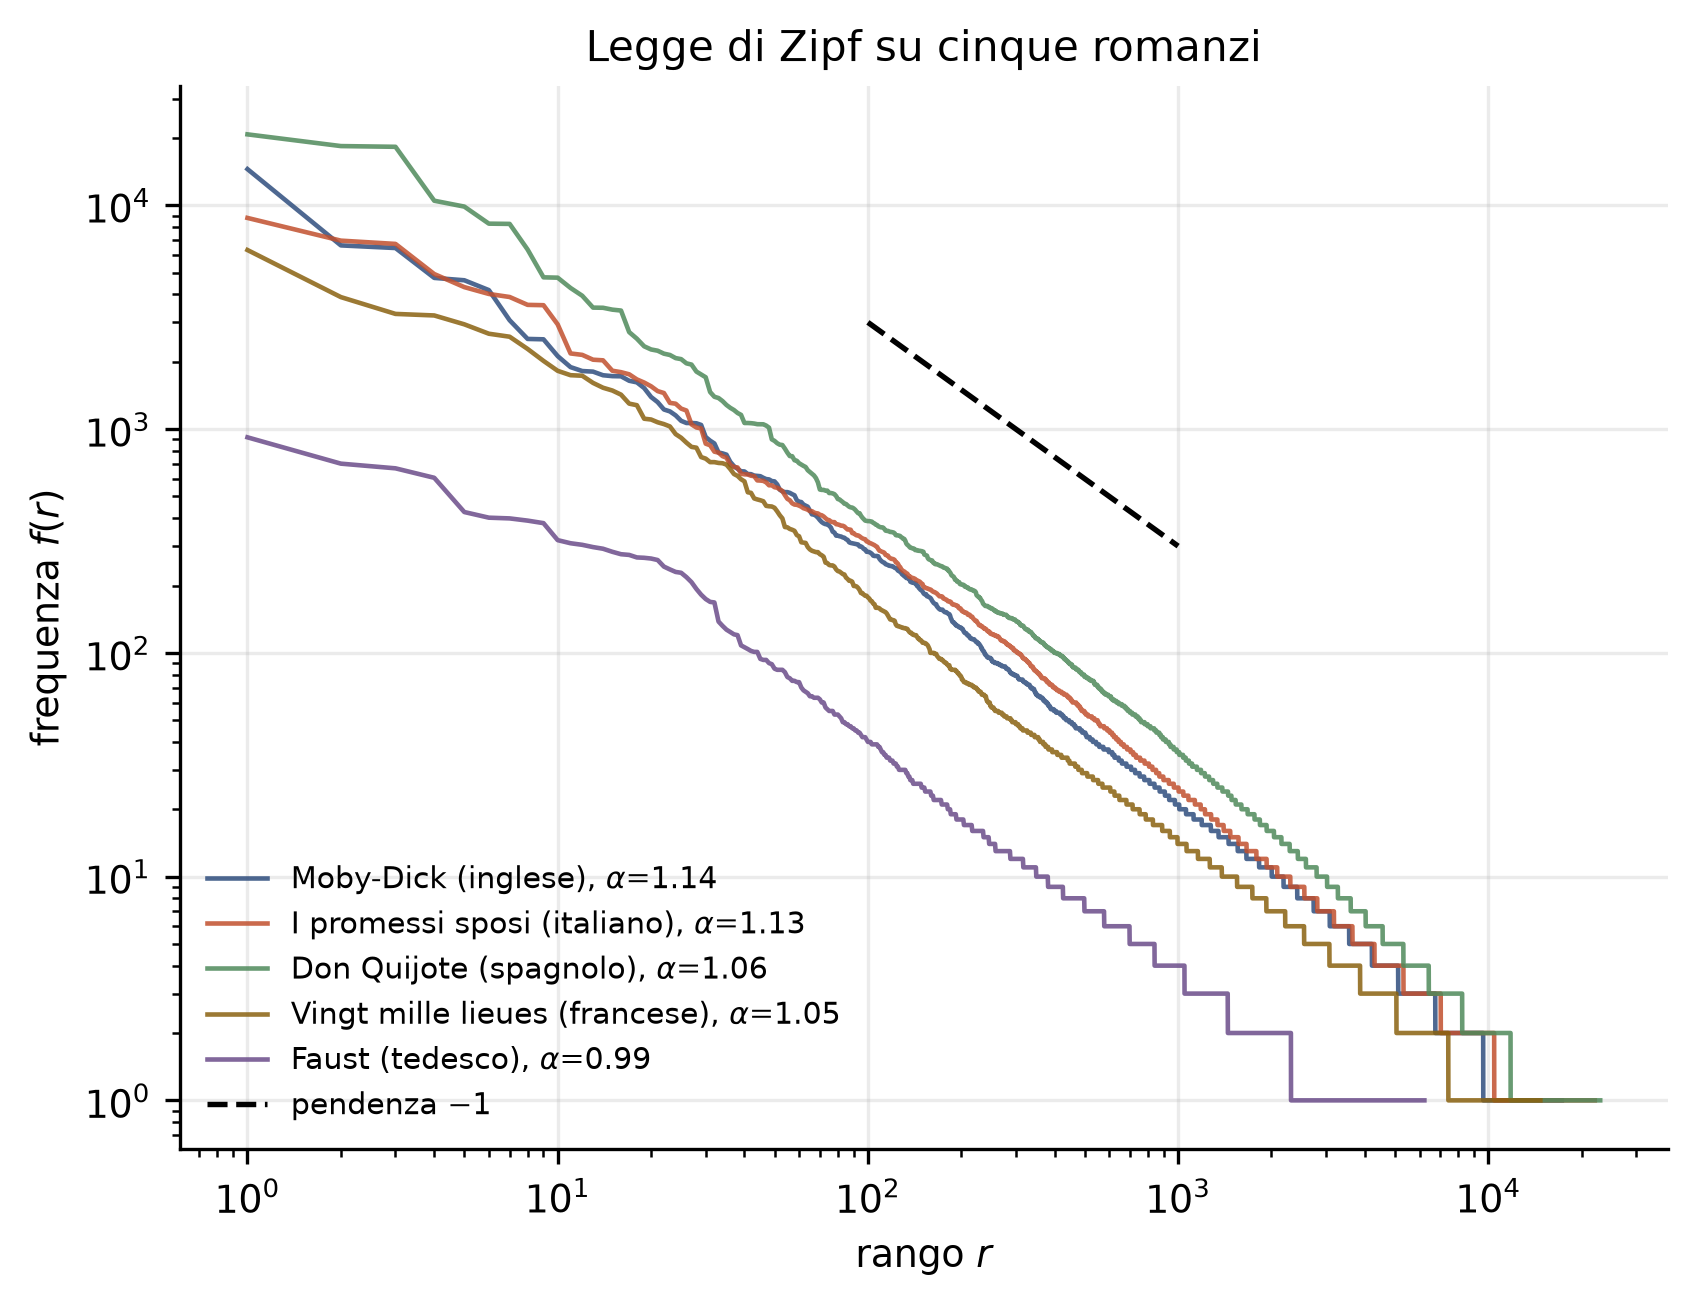
\includegraphics[width=0.82\textwidth]{figure/cap2_zipf_lingue.png}
  \caption{Relazione rango-frequenza per cinque romanzi in altrettante lingue,
  in coordinate bilogaritmiche. Gli esponenti riportati in legenda sono stimati
  per regressione ai minimi quadrati nella finestra di ranghi
  $10^2 \le r \le 10^3$, la stessa impiegata in~\cite{lippi2019}. La retta
  tratteggiata ha pendenza $-1$ ed è riportata come riferimento visivo.}
  \label{fig:zipf}
\end{figure}

Il parametro $\alpha$ risulta positivo e prossimo a 1 nella grande maggioranza
delle lingue esaminate, comprese quelle estinte e quelle costruite
artificialmente. Valori di
$\alpha$ più alti sono sintomo di un vocabolario più povero, poiché un numero
minore di parole esaurisce la maggior parte del testo; valori più bassi
segnalano al contrario una presenza più marcata di parole rare.

I valori misurati sulle cinque opere della Figura~\ref{fig:zipf} sono raccolti
nella Tabella~\ref{tab:zipf-misure}, accanto ai valori medi per lingua riportati
in~\cite{mikhaylovskiy2025zipf} su un corpus di sei opere letterarie in cinque
lingue.

\begin{table}[htbp]
\centering
\small
\begin{tabular}{@{}llrrr@{}}
\toprule
Opera & Lingua & Parole & $|\mathcal{D}|$ & $\alpha$ \\
\midrule
Moby-Dick               & inglese   & \num{219081} & \num{17258} & 1.14 \\
I promessi sposi        & italiano  & \num{239353} & \num{22040} & 1.13 \\
Don Quijote             & spagnolo  & \num{383633} & \num{22943} & 1.06 \\
Vingt mille lieues sous les mers & francese & \num{148923} & \num{14716} & 1.05 \\
Faust                   & tedesco   & \num{30959}  & \num{6221}  & 0.99 \\
\bottomrule
\end{tabular}
\caption{Esponente di Zipf misurato sulle cinque opere della
Figura~\ref{fig:zipf}, con il numero di occorrenze e la dimensione del
dizionario. La stima è condotta sui ranghi $10^2$--$10^3$.}
\label{tab:zipf-misure}
\end{table}

\begin{table}[htbp]
\centering
\small
\begin{tabular}{@{}lcccc@{}}
\toprule
& \multicolumn{2}{c}{$\alpha$ (Zipf)} & \multicolumn{2}{c}{$\gamma_H$ (Heaps)} \\
\cmidrule(lr){2-3}\cmidrule(lr){4-5}
Lingua & parole & token & parole & token \\
\midrule
inglese  & $0.952 \pm 0.072$ & $0.985 \pm 0.054$ & $0.809 \pm 0.027$ & $0.802 \pm 0.024$ \\
tedesco  & $0.959 \pm 0.054$ & $1.024 \pm 0.042$ & $0.846 \pm 0.031$ & $0.793 \pm 0.028$ \\
russo    & $1.043 \pm 0.077$ & $1.009 \pm 0.067$ & $0.916 \pm 0.049$ & $0.805 \pm 0.025$ \\
spagnolo & $0.962 \pm 0.030$ & $1.016 \pm 0.035$ & $0.842 \pm 0.025$ & $0.798 \pm 0.028$ \\
francese & $0.963 \pm 0.033$ & $0.989 \pm 0.042$ & $0.843 \pm 0.020$ & $0.801 \pm 0.018$ \\
\bottomrule
\end{tabular}
\caption{Esponenti medi per lingua riportati in~\cite{mikhaylovskiy2025zipf},
misurati su sei opere letterarie per ciascuna lingua, a livello di parola e di
token. In quel lavoro $\alpha$ è stimato sulla rappresentazione
cumulata della distribuzione anziché sulla relazione rango-frequenza; i due
stimatori coincidono soltanto nel limite $\alpha \to 1$, e i valori non vanno
quindi confrontati direttamente con quelli della
Tabella~\ref{tab:zipf-misure}.}
\label{tab:zipf-letteratura}
\end{table}

Sui testi reali si osservano deviazioni sistematiche dalla~\eqref{eq:zipf}. Su
corpora molto ampi l'esponente resta prossimo a 1 soltanto per le prime migliaia
di parole, mentre la coda continua a seguire una legge di potenza ma con
esponente maggiore~\cite{piantadosi2014}. Le parole più frequenti, inoltre,
mostrano frequenze leggermente inferiori a quelle previste: una deviazione che
Mandelbrot~\cite{mandelbrot1953} corregge introducendo un termine additivo nel
rango,
\begin{equation}
  f(r) \;\propto\; (r + c)^{-\alpha},
  \label{eq:mandelbrot}
\end{equation}
dove la costante $c > 0$ attenua la divergenza della legge di potenza ai ranghi
più bassi, spostando di fatto l'origine dell'asse dei ranghi e rendendo il fit
aderente anche nella regione delle parole più comuni.

\paragraph{Bontà del fit.}
Come si vedrà nei capitoli sperimentali, sui testi generati automaticamente
l'aderenza alla legge di potenza non è garantita. Il solo esponente non è
sufficiente a stabilirla, perché descrive la pendenza media della curva e non la
sua forma: una curva marcatamente incurvata in coordinate bilogaritmiche può
avere la stessa pendenza media di una retta, e restituire quindi un valore di
$\alpha$ del tutto ordinario pur non essendo una legge di potenza. Occorre
perciò una seconda quantità, che misuri quanto i dati si discostino dalla retta
interpolante.

Seguendo~\cite{mikhaylovskiy2025zipf}, la qualità del fit viene stimata con
l'errore percentuale assoluto medio
\begin{equation}
  \mathrm{MAPE} \;=\; \frac{1}{n}\sum_{i=1}^{n}
  \left| \frac{y_i - \hat{y}_i}{y_i} \right|,
  \label{eq:mape}
\end{equation}
dove $n$ è il numero di punti su cui è condotta la regressione, $y_i$ il valore
osservato e $\hat{y}_i$ quello previsto dalla retta interpolante in
corrispondenza dello stesso rango. Il MAPE è nullo per dati perfettamente
allineati e cresce al crescere della distanza relativa dalla retta;
essendo definito su scarti relativi, non dipende dall'unità di misura né
dall'ampiezza delle frequenze, e resta quindi confrontabile fra testi di
lunghezza diversa.

Sul corpus di testi letterari usato in~\cite{mikhaylovskiy2025zipf} il MAPE vale
in media $0.156$ con deviazione standard $0.077$. Nei capitoli sperimentali il
suo minimo in funzione della temperatura di generazione individuerà il regime in
cui il testo prodotto è più vicino a una legge di potenza.

% ---------------------------------------------------------------------
\subsection{Legge di Heaps}
\label{sec:heaps}

Studiando l'andamento di $|\mathcal{D}(t)|$ nei testi letterari emerge una
seconda regolarità, nota come legge di Heaps o, dal nome di chi la formulò per
primo~\cite{herdan1964}, di Herdan--Heaps:
\begin{equation}
  |\mathcal{D}(t)| \;\propto\; t^{\gamma_H}, \qquad \gamma_H \in [0,1] .
  \label{eq:heaps}
\end{equation}
Qui $t$ è la posizione nel testo, misurata in numero di parole,
$|\mathcal{D}(t)|$ la dimensione del dizionario parziale e $\gamma_H$
l'esponente di Heaps. I due estremi dell'intervallo corrispondono a due
comportamenti limite: $\gamma_H = 0$ descrive un dizionario che cessa di
crescere, cioè un testo che non introduce più parole nuove, mentre
$\gamma_H = 1$ descrive un dizionario che cresce proporzionalmente alla
lunghezza, cioè un testo in cui ogni parola è nuova. Poiché il dizionario non
può crescere più rapidamente del testo che lo contiene, si ha necessariamente
$|\mathcal{D}(t)| \le t$, e l'esponente non può eccedere l'unità.

La legge di Heaps quantifica dunque la capacità di un testo di rinnovare il
proprio vocabolario, ed è per questo particolarmente istruttiva se si torna alla
Tabella~\ref{tab:tre-regimi} del Capitolo~\ref{cap:introduzione}. Il primo
esempio, monotono e ripetitivo, cessa rapidamente di accrescere il dizionario;
l'ultimo, in cui i caratteri sono estratti a caso, produce quasi soltanto parole
nuove e fa crescere il dizionario senza saturare. La Figura~\ref{fig:heaps}
mostra le curve dei due casi limite accanto a quelle di tre testi letterari.

\begin{figure}[htbp]
  \centering
  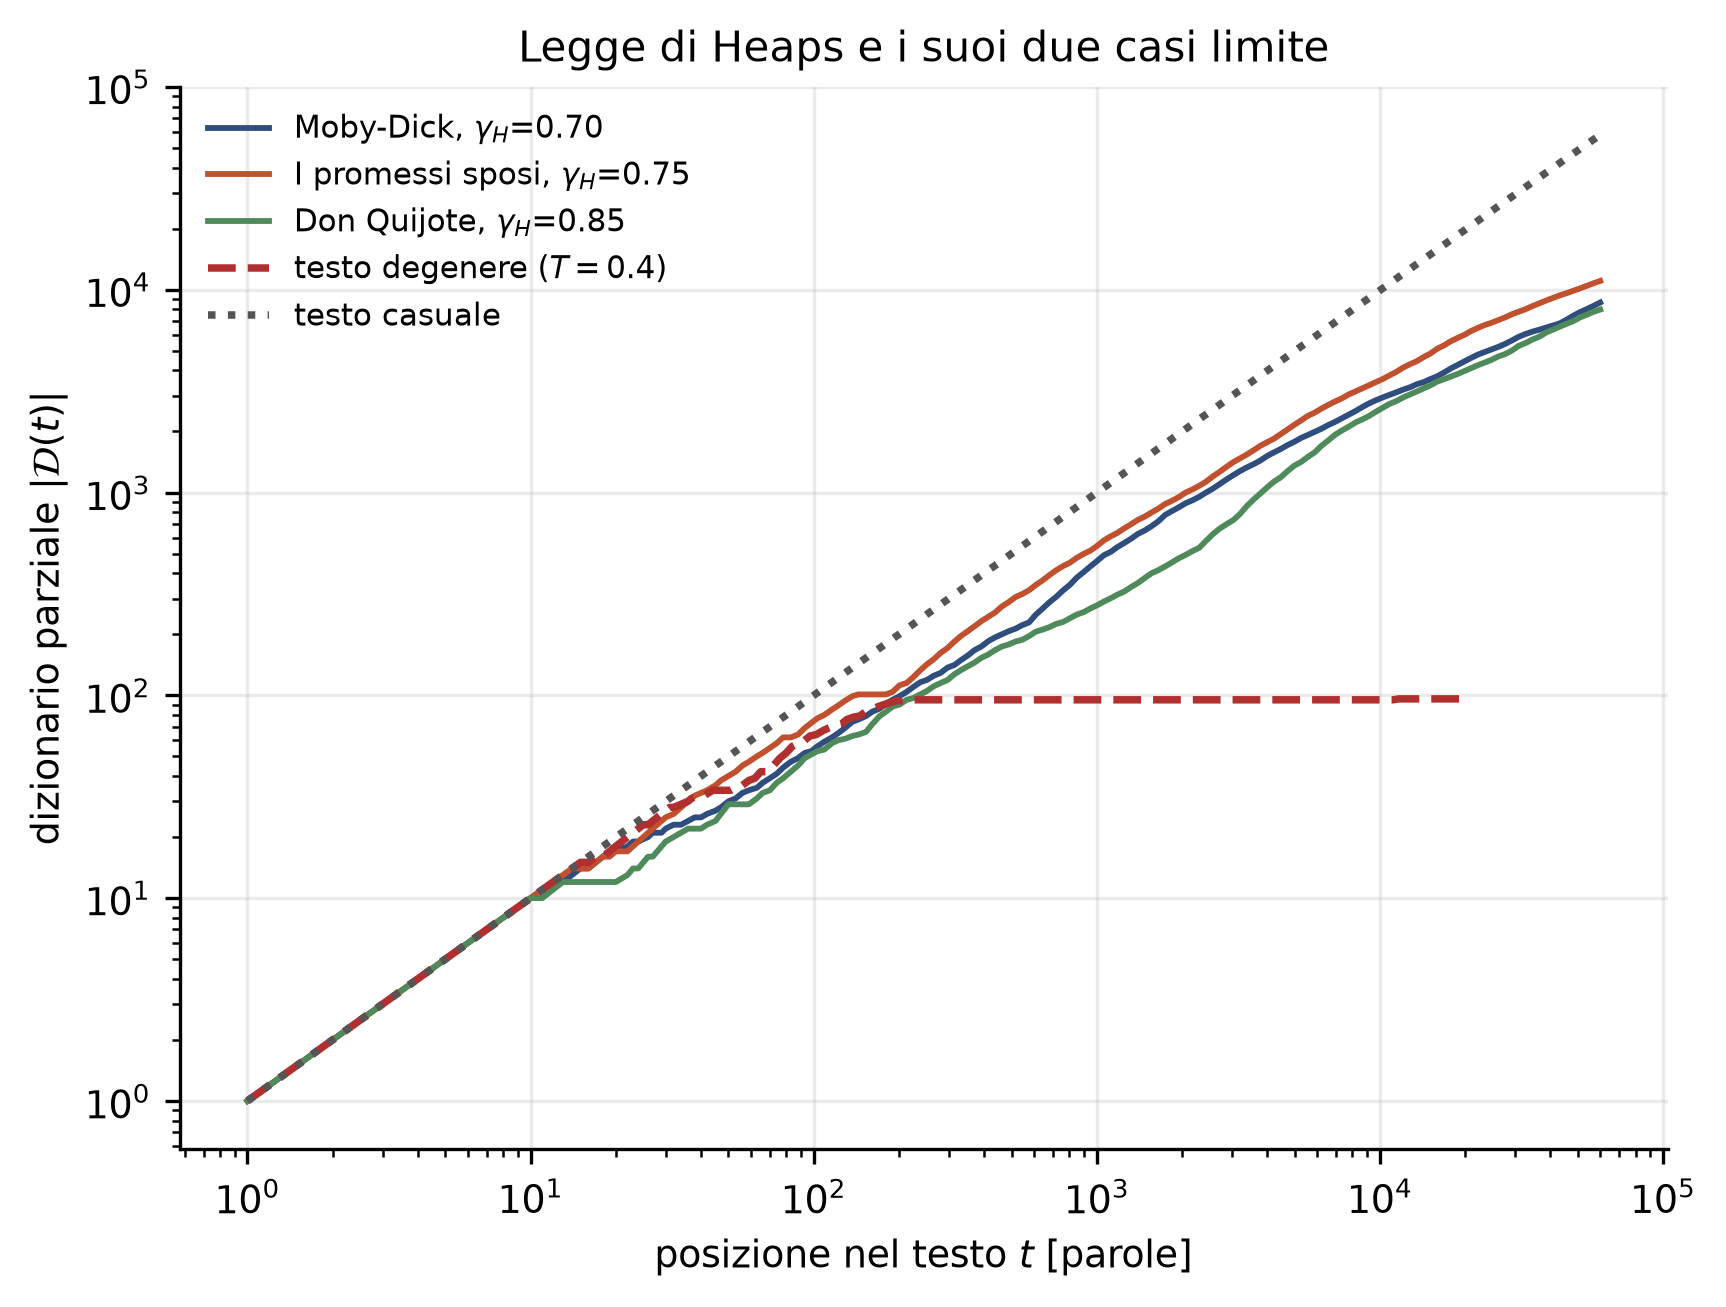
\includegraphics[width=0.82\textwidth]{figure/cap2_heaps_confronto.png}
  \caption{Crescita del dizionario parziale in coordinate bilogaritmiche. Le tre
  curve continue sono testi letterari, con esponente stimato nella regione
  $t > 1000$. La curva tratteggiata è il campione generato a $T = 0.4$ già
  riportato nella Tabella~\ref{tab:tre-regimi}: dopo circa un centinaio di
  parole entra in un ciclo di ripetizione e il dizionario si arresta. La curva
  punteggiata è una sequenza di caratteri casuali, in cui ogni parola è nuova e
  la crescita è esattamente lineare.}
  \label{fig:heaps}
\end{figure}

L'esponente stimato dipende inoltre dall'intervallo su cui viene condotta la
regressione, e quindi dalla lunghezza del testo analizzato. La
Figura~\ref{fig:heaps-finito} mostra l'effetto su tre opere: ripetendo la stima
su prefissi via via più lunghi della stessa opera, $\gamma_H$ decresce in modo
sistematico, di oltre un decimo fra $10^4$ e $10^5$ parole. Il fenomeno è la
prima manifestazione degli effetti di dimensione finita discussi in modo
generale nel §\ref{sec:lunghezza}, ed è già segnalato
in~\cite{mikhaylovskiy2025zipf}, dove si osserva che per $\alpha$ prossimo a 1
la crescita del dizionario è descritta meglio dalla forma $t/\ln t$ che da una
pura legge di potenza. Ai valori di $N$ più bassi la regressione si appoggia a
un intervallo troppo corto e può restituire stime superiori a 1, incompatibili
con il limite teorico: è un artefatto della finestra di fit, non una proprietà
del testo.

\begin{figure}[htbp]
  \centering
  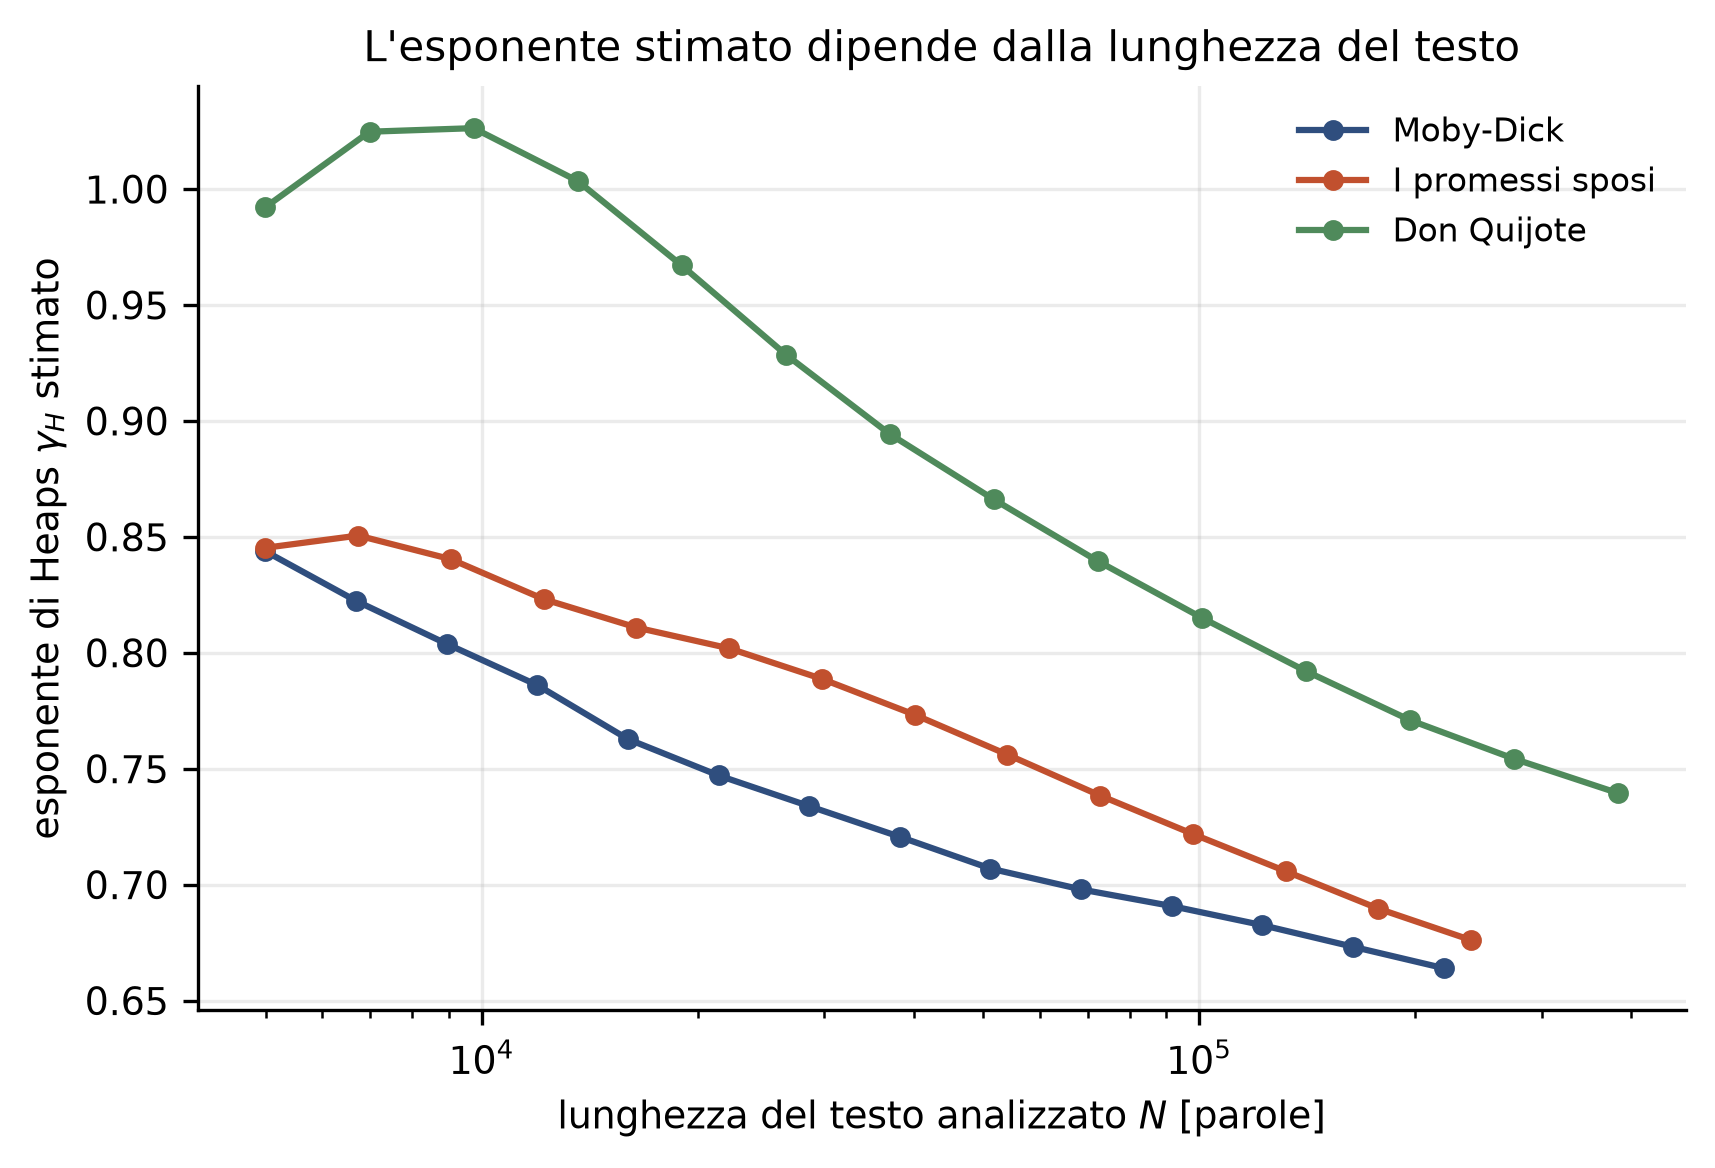
\includegraphics[width=0.78\textwidth]{figure/cap2_heaps_dimensione_finita.png}
  \caption{Esponente di Heaps stimato su prefissi di lunghezza crescente, per tre
  opere in tre lingue diverse, con regressione condotta nella regione $t > 1000$.
  La deriva è sistematica e comune a tutte e tre, ed è quindi una proprietà dello
  stimatore e non di una particolare opera: confrontare esponenti misurati su
  testi di lunghezza diversa non è lecito. Il §\ref{sec:scelte} riprende
  l'effetto su una sola opera, misurandone però l'entità su tutti gli stimatori
  impiegati in questa tesi.}
  \label{fig:heaps-finito}
\end{figure}

\paragraph{Il descrittore $R$.}
Sui testi generati automaticamente la difficoltà è più radicale. A bassa
temperatura di generazione il modello entra in un ciclo di ripetizione e cessa
di produrre parole nuove: la curva $|\mathcal{D}(t)|$ diventa piatta e
la~\eqref{eq:heaps} perde significato. Ad alta temperatura si verifica il caso
opposto, con quasi ogni parola nuova e curva prossima alla linearità. In
entrambe le situazioni la stima di $\gamma_H$ restituisce un numero privo di
contenuto, come mostrano le due curve estreme della Figura~\ref{fig:heaps}.

Per questa ragione in~\cite{mikhaylovskiy2025zipf} viene introdotto un
descrittore che resta definito in ogni regime. Detti $\mathcal{D}_1$ il
dizionario della prima metà del testo e $\mathcal{D}_2$ quello della seconda, si
pone
\begin{equation}
  R \;=\; \frac{|\mathcal{D}_2 \setminus \mathcal{D}_1|}{|\mathcal{D}_1|},
  \label{eq:R}
\end{equation}
cioè il rapporto fra il numero di parole che compaiono per la prima volta nella
seconda metà del testo e il numero di quelle che compaiono per la prima volta
nella prima. Un testo degenerato ha $R$ prossimo a zero, poiché la seconda metà
non introduce nulla di nuovo; un testo in cui ogni parola è nuova ha $R$
prossimo a uno. Sul corpus di opere letterarie intere usato
in~\cite{mikhaylovskiy2025zipf} il valore medio è $R = 0.17$ con deviazione
standard $0.05$.


% ---------------------------------------------------------------------
\section{Correlazioni a lungo raggio}
\label{sec:lrc}

Sia la legge di Zipf sia quella di Heaps ignorano l'ordine dei simboli. Per la
prima l'affermazione è immediata: la~\eqref{eq:zipf} dipende soltanto dai
conteggi delle parole, e un rimescolamento del testo li lascia invariati. Per la
seconda l'invarianza è meno diretta: rimescolando il testo la curva
$|\mathcal{D}(t)|$ cambia realizzazione, perché cambia l'ordine in cui le
parole compaiono per la prima volta, ma il suo andamento medio resta lo stesso, e con esso l'esponente
$\gamma_H$. Entrambe sono quindi proprietà del vocabolario, non della sequenza.

Per misurare le proprietà che dipendono dall'ordine occorre estrarre dal testo
un segnale, cioè una successione finita di valori reali, e studiarne le
correlazioni a scale diverse. La costruzione del segnale non è unica, e ogni
scelta mette in luce aspetti differenti: si può codificare la posizione delle
singole lettere o di classi di lettere, quella delle parole o di classi
grammaticali, oppure la lunghezza delle frasi. In tutti i casi si osserva che il
linguaggio esibisce correlazioni a lungo raggio, con una struttura che si
estende su molti ordini di grandezza~\cite{altmann2012,montemurro2002}.

% ---------------------------------------------------------------------
\subsection{Funzione di autocorrelazione}
\label{sec:acf}

Data una successione $x_1,\dots,x_N$, la funzione di autocorrelazione a distanza
$s$ è
\begin{equation}
  c(s) \;=\; \langle x_n x_{n+s}\rangle
  - \langle x_n\rangle\langle x_{n+s}\rangle ,
  \label{eq:acf}
\end{equation}
dove $\langle\cdot\rangle$ indica la media su tutte le posizioni $n$ compatibili
con la distanza $s$. La forma funzionale di $c(s)$ distingue i regimi di
correlazione.

Se i valori non sono correlati, $c(s)$ è identicamente nulla per $s \neq 0$. Se
$c(s)$ decade esponenzialmente,
$c(s) \sim e^{-s/s_0}$, il segnale si dice correlato a corto raggio: la costante
$s_0$ ha le dimensioni di una distanza e ne fissa la scala caratteristica, nel
senso che oltre poche volte $s_0$ la correlazione è numericamente
indistinguibile da zero. Esiste dunque una distanza tipica oltre la quale due
porzioni di segnale sono indipendenti, e il sistema non possiede struttura al di
là di essa.

Si dice invece che il segnale è correlato a lungo raggio quando il decadimento
segue la legge di potenza
\begin{equation}
  c(s) \;\sim\; s^{-\theta},
  \label{eq:acf-power}
\end{equation}
con $0<\theta<1$. In questo caso non esiste alcuna scala privilegiata: la
funzione~\eqref{eq:acf-power} è invariante di scala, cioè riscalare $s$ di un
fattore costante riscala $c$ di un fattore costante senza modificarne la forma,
e un certo grado di correlazione persiste a tutte le distanze.\footnote{L'esponente
qui indicato con $\theta$ è denotato con $\beta$ in~\cite{altmann2012} e con
$\gamma$ in altra parte della letteratura. Il simbolo è stato cambiato per
evitare la collisione con l'esponente di Heaps e con quello introdotto
nella~\eqref{eq:sigma}.}

La stima diretta di $\theta$ dalla~\eqref{eq:acf-power} è però problematica. Il
segnale è affetto da rumore e, soprattutto, da tendenze di origine esterna che
non sono oggetto di interesse: se la media $\langle x_n\rangle$ differisce fra
la prima e la seconda metà del segnale, come accade proprio quando le
correlazioni sono forti, la~\eqref{eq:acf} risulta distorta. L'esponente va
quindi stimato per via indiretta, e le due sottosezioni seguenti presentano i
due metodi impiegati in questa tesi.

% ---------------------------------------------------------------------
\subsection{Indicatore integrato}
\label{sec:integrato}

Il primo metodo è quello adottato da Altmann, Cristadoro e Degli
Esposti~\cite{altmann2012}, e si applica a segnali binari. Sia dato un testo
come successione simbolica $s = (s_1,\dots,s_N)$. Si definisce una condizione
locale $\mathcal{A}$ che genera la successione binaria
\begin{equation}
  x_k \;=\;
  \begin{cases}
    1 & \text{se $\mathcal{A}$ è soddisfatta in posizione $k$},\\
    0 & \text{altrimenti}.
  \end{cases}
  \label{eq:osservabile}
\end{equation}
L'osservabile può essere la presenza di una data lettera, di una data parola,
oppure l'appartenenza a una classe: per esempio se la lettera in posizione $k$ è
una vocale. L'unità di misura della distanza è il numero di simboli del livello
considerato, ed è questa scelta a rendere confrontabili fra loro una successione
di lettere e una di parole.

Posto
\begin{equation}
  X(t) \;=\; \sum_{j \le t} x_j ,
  \label{eq:conteggio}
\end{equation}
cioè il numero di occorrenze osservate nelle prime $t$ posizioni, si studia la
crescita della varianza del conteggio
\begin{equation}
  \sigma_X^2(t) \;=\; \langle X(t)^2\rangle - \langle X(t)\rangle^2
  \;\simeq\; t^{\gamma}, \qquad \gamma = 2 - \theta .
  \label{eq:sigma}
\end{equation}
La quantità $\sigma_X^2$ è, per costruzione, una somma delle correlazioni a
tutte le distanze inferiori a $t$, e come tale è numericamente assai più stabile
della~\eqref{eq:acf} stimata punto per punto.

Il discrimine fra correlazioni a corto e a lungo raggio non è l'ampiezza di
$c(s)$, ma la sua sommabilità. La~\eqref{eq:conteggio} è formalmente il
cammino percorso da un camminatore che a ogni passo avanza di $x_j$: se i passi
sono indipendenti, o abbastanza rapidamente decorrelati perché $\sum_s c(s)$
converga, vale il teorema del limite centrale e la varianza del cammino cresce
proporzionalmente al numero di passi. Si ha allora diffusione normale,
$\gamma = 1$, esattamente come per il moto browniano. Se invece la somma
diverge, cioè se $\theta \le 1$, i passi restano correlati a ogni scala, il
camminatore tende a proseguire nella direzione già intrapresa e si allontana
dall'origine più rapidamente: la diffusione è anomala e $1 < \gamma < 2$. Il
valore $\gamma = 1$ costituisce dunque il riferimento nullo di tutte le misure
di questo tipo.

La stima di $\gamma$ risente di effetti di tempo finito che la fanno
sottostimare~\cite{altmann2012}: tutti i valori riportati nei capitoli
sperimentali vanno letti come limiti inferiori.

% ---------------------------------------------------------------------
\subsection{Detrended fluctuation analysis}
\label{sec:dfa}

Il secondo metodo è la \emph{detrended fluctuation analysis}, introdotta da
Peng et al.~\cite{peng1994} e applicata ai testi generati automaticamente
in~\cite{lippi2019}. Rispetto all'indicatore integrato presenta il vantaggio
di rimuovere le tendenze locali, e risulta quindi applicabile anche a segnali
non stazionari, cioè segnali le cui proprietà statistiche, tipicamente la
media $\langle x_n \rangle$ o la varianza, non sono costanti lungo la
successione ma derivano lentamente da un estremo all'altro.

La distinzione fra tendenza e correlazione è essenziale, e non riguarda solo
l'origine delle due. Una tendenza è una deriva sistematica e regolare del valore
medio, sovrapposta al segnale da una causa esterna al sistema; una correlazione
è invece una proprietà statistica interna, che lega fra loro le fluttuazioni
attorno a quel valore medio. Il problema pratico è che entrambe producono lo
stesso effetto sulla~\eqref{eq:acf}, gonfiandola a grandi distanze, ed è quindi
necessario eliminare le prime per misurare le seconde. Si potrebbe pensare
sufficiente sottrarre una media mobile di ampiezza fissata, ma in questo modo si
introdurrebbe artificialmente nei dati proprio quella ampiezza come scala
caratteristica, distruggendo le altre.

Il segnale viene costruito codificando ogni carattere del testo con il proprio
rango di frequenza: al carattere più frequente si associa 1, al secondo 2, e
così via. Seguendo~\cite{lippi2019} la codifica avviene a livello di carattere e
conserva punteggiatura, cifre, maiuscole e lettere accentate. Ottenuta la
successione $x_i$ con $i = 1,\dots,N$, la procedura si articola in quattro
passi, qui presentati nella formulazione di~\cite{kantelhardt2001}.

\begin{enumerate}
  \item Si determina il profilo
    \begin{equation}
      Y(i) \;=\; \sum_{k=1}^{i}\bigl(x_k - \langle x\rangle\bigr),
      \label{eq:dfa-profilo}
    \end{equation}
    cioè lo scarto cumulato dalla media. La sottrazione della media non è
    strettamente necessaria, poiché verrebbe comunque eliminata dal detrending.
  \item Si divide il profilo in $N_s = \lfloor N/s \rfloor$ segmenti disgiunti
    di lunghezza $s$.
  \item In ciascun segmento si interpola ai minimi quadrati la tendenza locale,
    ottenendo il polinomio $Y_s(i)$ che approssima il profilo entro quel
    segmento. L'ordine del polinomio determina l'ordine delle tendenze rimosse:
    una DFA di ordine $n$ elimina le tendenze polinomiali fino al grado $n$. In
    questa tesi si impiega l'ordine 1, che rimuove le tendenze lineari locali;
    la robustezza dei risultati rispetto a questa scelta è verificata nel
    §\ref{sec:robustezza}.
  \item Si calcola lo scarto quadratico medio del profilo dalla propria
    tendenza locale, mediando su tutti i segmenti, e si ottiene la funzione di
    fluttuazione
    \begin{equation}
      F(s) \;=\; \left(\frac{1}{N}\sum_{i=1}^{N}
      \bigl(Y(i) - Y_s(i)\bigr)^2\right)^{1/2}.
      \label{eq:dfa-F}
    \end{equation}
\end{enumerate}

La fluttuazione cresce con la lunghezza dei segmenti $s$ e, per un segnale
correlato a lungo raggio, segue la legge di potenza
\begin{equation}
  F(s) \;\sim\; s^{\alpha_{\mathrm{DFA}}} .
  \label{eq:dfa-alpha}
\end{equation}
Per un segnale scorrelato, o correlato a corto raggio, si ha
$\alpha_{\mathrm{DFA}} = 1/2$. Valori superiori indicano correlazioni
persistenti: una fluttuazione positiva tende a essere seguita da un'altra
fluttuazione positiva, e il segnale conserva memoria della propria direzione.
Valori inferiori indicano correlazioni antipersistenti, in cui una fluttuazione
positiva tende a essere seguita da una negativa e il segnale tende a tornare
sui propri passi. Un cammino aleatorio dà $\alpha_{\mathrm{DFA}} = 3/2$: i suoi
incrementi sono scorrelati, ma la successione che ne risulta accumula ogni
deviazione senza riassorbirla, e le fluttuazioni crescono di conseguenza molto
più in fretta. Sul testo letterario di riferimento~\cite{lippi2019} riporta
$\alpha_{\mathrm{DFA}} \simeq 0.65$, contro $0.50$ misurato sulla sua versione
rimescolata: nettamente sopra il riferimento scorrelato e nettamente sotto
quello del cammino aleatorio.

% ---------------------------------------------------------------------
\subsection{Relazione fra i due metodi}
\label{sec:ponte}

I due metodi introdotti misurano la stessa proprietà, e i rispettivi esponenti
sono legati da una relazione semplice. Applicata alla medesima successione,
la~\eqref{eq:dfa-F} coincide, a meno del detrending, con la deviazione standard
del profilo alla scala $s$, cioè $F(s) \simeq \sigma_X(s)$. Elevando al quadrato
e usando la~\eqref{eq:sigma} si ottiene $F(s)^2 \simeq s^{\gamma}$, da cui
\begin{equation}
  \alpha_{\mathrm{DFA}} \;=\; \frac{\gamma}{2} \;=\; 1 - \frac{\theta}{2} .
  \label{eq:ponte}
\end{equation}
La stessa relazione, ricavata per altra via, è riportata
in~\cite{kantelhardt2001}. Nella~\eqref{eq:ponte} $\gamma$ è l'esponente di
crescita della varianza del conteggio definito nella~\eqref{eq:sigma}, mentre
$\theta$ è l'esponente di decadimento dell'autocorrelazione definito
nella~\eqref{eq:acf-power}; i tre esponenti sono dunque tre modi equivalenti di
esprimere la stessa proprietà del segnale.

La~\eqref{eq:ponte} costituisce il ponte fra le due parti sperimentali della
tesi: la diffusione normale $\gamma = 1$, riferimento nullo dell'analisi di
burstiness, corrisponde esattamente al valore $\alpha_{\mathrm{DFA}} = 1/2$,
riferimento nullo dell'analisi sui testi generati. Le due misure non coincidono
esattamente sui dati, poiché la detrended fluctuation analysis rimuove le
tendenze locali mentre l'indicatore integrato no; la differenza fra i due
risultati è informativa proprio quando il segnale non è stazionario.

Un caso limite si presenta con frequenza nei testi generati a bassa
temperatura. Se il testo degenera in un ciclo di ripetizione,
la successione $x_i$ diventa quasi periodica e il profilo~\eqref{eq:dfa-profilo}
oscilla invece di allontanarsi dall'origine: la fluttuazione satura oltre la
lunghezza del periodo e $\alpha_{\mathrm{DFA}}$ scende verso zero. Un esponente
molto basso non segnala quindi assenza di struttura, ma struttura periodica, e
va interpretato congiuntamente a un indicatore diretto di ripetizione.


% ---------------------------------------------------------------------
\section{Burstiness e statistica degli intervalli}
\label{sec:burst}

Le sezioni precedenti permettono di stabilire se un testo possieda correlazioni
a lungo raggio. Questa sezione introduce gli strumenti necessari a stabilire
l'origine di tali correlazioni, che è la domanda posta in~\cite{altmann2012} e
ripresa nella seconda parte sperimentale.

Il punto di partenza è un'osservazione elementare sulla distribuzione delle
parole lungo il testo. Non tutte le parole si distribuiscono allo stesso modo:
alcune ricorrono in modo pressoché uniforme dall'inizio alla fine, altre si
addensano nelle sezioni che trattano l'argomento cui appartengono e sono quasi
assenti altrove. La Figura~\ref{fig:barcode} rende visibile la differenza. Ogni
barra verticale segna una posizione in cui la parola compare; nel primo pannello
la parola è un articolo, nel secondo il nome di un personaggio.

\begin{figure}[htbp]
  \centering
  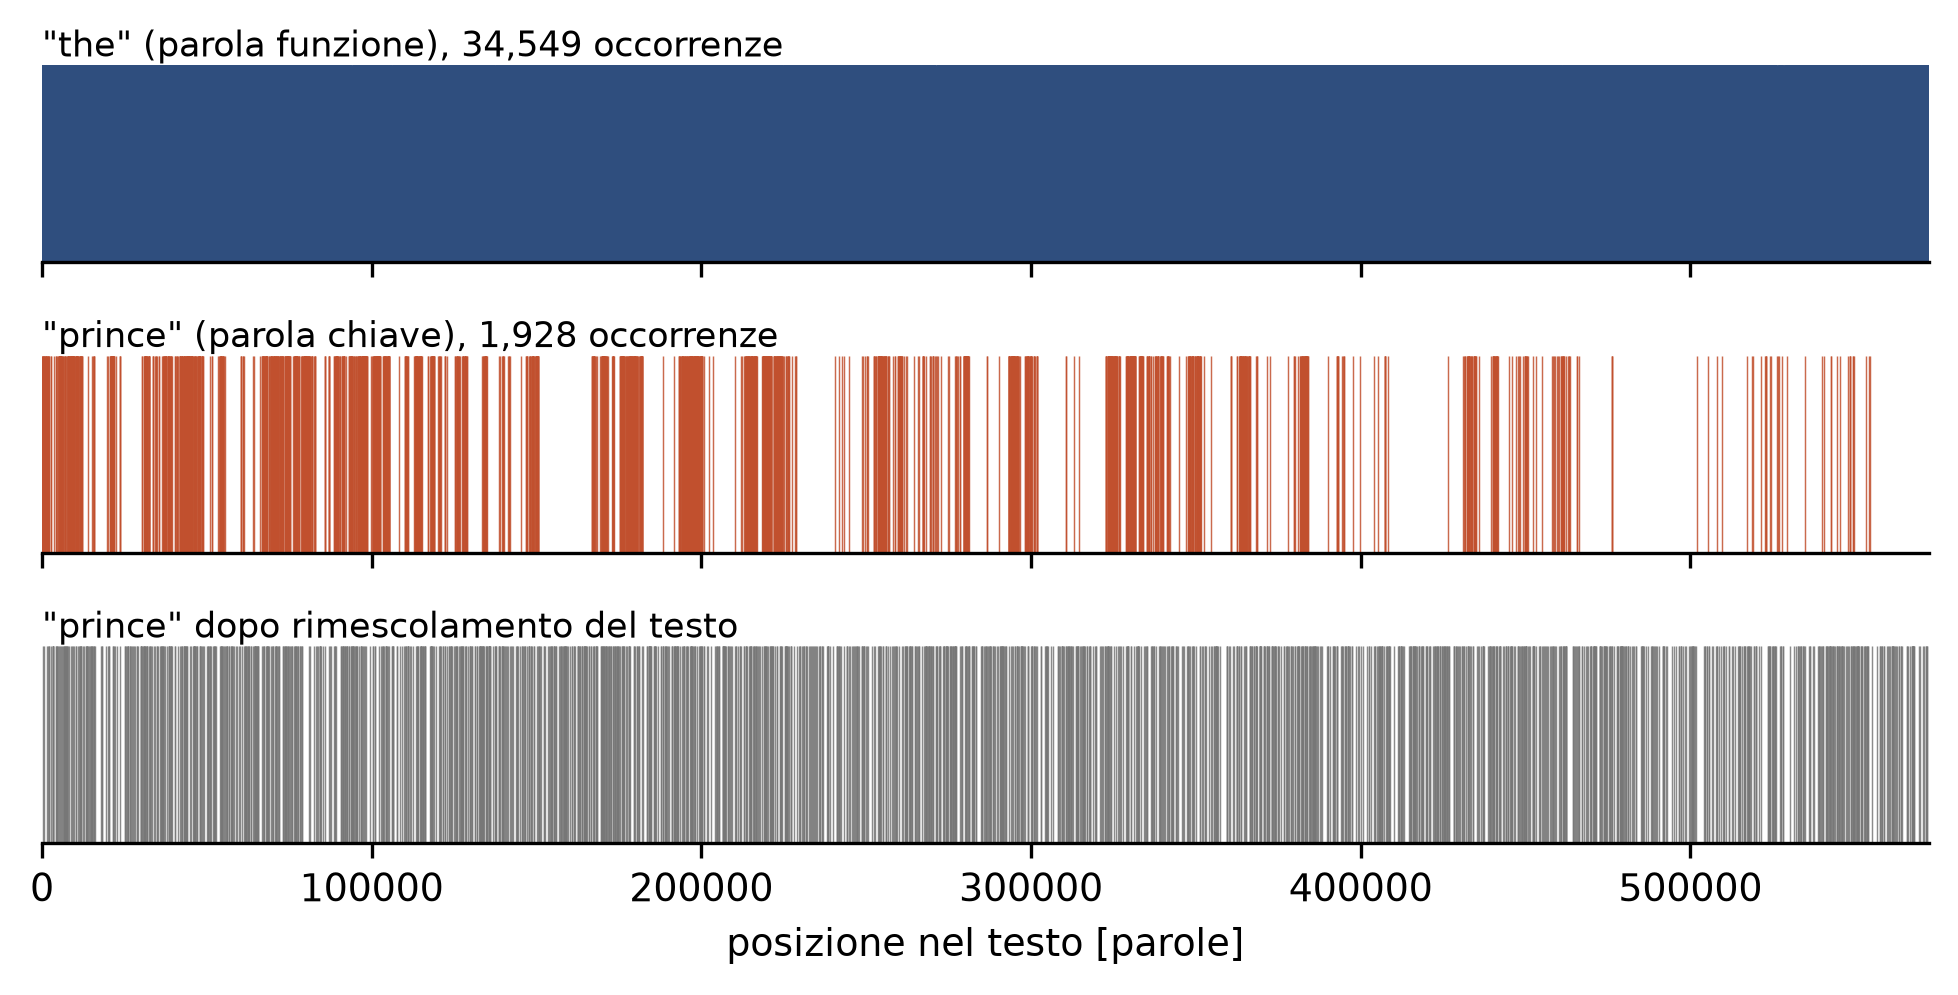
\includegraphics[width=\textwidth]{figure/cap2_burstiness_barcode.png}
  \caption{Posizioni di occorrenza di due parole in \emph{Guerra e pace}. La
  parola funzione \emph{the} riempie il testo in modo uniforme e il pannello
  appare come una banda piena. La parola chiave \emph{prince} si addensa invece
  in gruppi separati da lunghi vuoti, che corrispondono alle porzioni di romanzo
  in cui il personaggio non compare. Il terzo pannello riporta le occorrenze di
  \emph{prince} dopo aver rimescolato le parole del testo: i conteggi sono
  identici, ma i gruppi scompaiono. La struttura visibile nel secondo pannello
  è dunque una proprietà dell'ordine, non delle frequenze.}
  \label{fig:barcode}
\end{figure}

Il fenomeno illustrato dal secondo pannello prende il nome di
\emph{burstiness}: le occorrenze non sono sparse indipendentemente, ma
raggruppate in raffiche separate da intervalli lunghi. Il terzo pannello mostra
perché si tratti di una proprietà dell'ordine e non del vocabolario: il
rimescolamento conserva esattamente il numero di occorrenze, e con esso la legge
di Zipf, ma distrugge la struttura.

Per quantificare il fenomeno si torna alla successione binaria definita
nella~\eqref{eq:osservabile} e si considerano gli intervalli
$\tau_1, \tau_2, \dots$ fra occorrenze consecutive, cioè le distanze in numero
di simboli fra un $1$ e il successivo. La loro distribuzione di probabilità
viene indicata con $p(\tau)$ ed è l'oggetto centrale di questa sezione: tutta
l'informazione sull'ordine che il conteggio delle occorrenze non cattura è
contenuta in $p(\tau)$ e nelle correlazioni fra intervalli successivi.

Il termine di paragone naturale è il processo di Poisson, cioè il processo in
cui ogni posizione ha la stessa probabilità di ospitare un'occorrenza,
indipendentemente da tutte le altre. È il modello del «nessuna struttura»: se le
occorrenze di \emph{prince} fossero poissoniane, il secondo pannello della
Figura~\ref{fig:barcode} sarebbe indistinguibile dal terzo. Per un processo di
Poisson gli intervalli sono distribuiti esponenzialmente e indipendenti fra
loro, e si dimostra che la loro deviazione standard eguaglia la media,
$\sigma_\tau = \langle\tau\rangle$.

Si misura quindi la burstiness con il coefficiente di variazione
\begin{equation}
  \mathrm{cv} \;=\; \frac{\sigma_\tau}{\langle\tau\rangle},
  \label{eq:cv}
\end{equation}
pari a 1 nel caso poissoniano, maggiore di 1 quando le occorrenze si addensano
in raffiche separate da vuoti lunghi e minore di 1 quando sono distribuite in
modo più regolare di quanto il caso comporti. Una misura equivalente, ma
limitata all'intervallo $[-1,1]$ e quindi più comoda per il confronto fra
sequenze diverse, è l'indice proposto da Goh e Barabási~\cite{goh2008},
\begin{equation}
  B \;=\; \frac{\sigma_\tau - \langle\tau\rangle}
                {\sigma_\tau + \langle\tau\rangle} .
  \label{eq:goh}
\end{equation}

% ---------------------------------------------------------------------
\subsection{Le due origini delle correlazioni}
\label{sec:origini}

Il contributo centrale di~\cite{altmann2012} consiste nell'osservare che una
varianza del conteggio che cresce più che linearmente può avere due origini
distinte. Il legame è fornito dallo spettro di potenza a frequenza nulla.

Lo spettro di potenza $S(\omega)$ di una successione descrive come la sua
varianza si distribuisce fra le diverse frequenze $\omega$, ed è la trasformata
di Fourier della funzione di autocorrelazione. Il valore a frequenza nulla,
$S(0)$, raccoglie il contributo delle fluttuazioni più lente, quelle su scale
comparabili con la lunghezza dell'intera successione: è quindi la quantità che
diverge esattamente quando esistono correlazioni a lungo raggio, e che resta
finita quando le correlazioni sono sommabili. Per una successione di occorrenze
descritta dagli intervalli $\tau_i$ vale
\begin{equation}
  S(0) \;=\; \frac{\sigma_\tau^2}{\langle\tau\rangle^3}
  \left(1 + 2\sum_{k\ge1} c_\tau(k)\right),
  \label{eq:eq4}
\end{equation}
dove $c_\tau(k)$ è l'autocorrelazione della successione degli intervalli, cioè
la correlazione fra $\tau_i$ e $\tau_{i+k}$.

La~\eqref{eq:eq4} è il perno dell'intera analisi, perché mostra che $S(0)$ può
divergere in due modi indipendenti. Il primo è la divergenza di $\sigma_\tau$,
cioè una coda pesante di $p(\tau)$: il testo contiene vuoti così lunghi che la
varianza degli intervalli non converge. Il secondo è la non sommabilità di
$c_\tau(k)$, cioè il fatto che gli intervalli siano essi stessi correlati fra
loro. Nella formula resta implicito che cosa questo comporti: $c_\tau(k) > 0$
significa che a un intervallo più lungo della media tende a seguirne un altro
più lungo della media, e quindi che i vuoti si
raggruppano fra loro invece di alternarsi ai riempimenti. Anche con una
$p(\tau)$ a varianza finita, un simile raggruppamento produce fluttuazioni
lente del conteggio e fa divergere la somma.

I due meccanismi sono distinti, perché l'uno riguarda quanto sono lunghi i
vuoti e l'altro come sono disposti, e la~\eqref{eq:eq4} da sola non li separa.

Nei testi reali, di lunghezza finita e con la coda tagliata
(§\ref{sec:coda}), nessuna delle due quantità diverge davvero: ciò che si
misura sono i loro analoghi a finestra finita, e i due null model del
§\ref{sec:null} servono appunto a separarli senza dover decidere quale delle
due divergenze sarebbe realizzata nel limite.

% ---------------------------------------------------------------------
\subsection{I null model A1 e A2}
\label{sec:null}

La separazione si ottiene con due rimescolamenti controllati, costruiti in modo
da distruggere selettivamente uno solo dei due meccanismi.

Il primo, indicato con A1, permuta gli zeri e gli uni della successione binaria.
Conserva soltanto il numero di occorrenze e distrugge tanto la coda di $p(\tau)$
quanto $c_\tau(k)$: è il rimescolamento già illustrato nel terzo pannello della
Figura~\ref{fig:barcode}. Ha funzione di controllo, poiché il risultato è noto a
priori: deve restituire un esponente $\hat\gamma_{A1}$ prossimo a 1, e un valore
diverso segnala un difetto della procedura di misura prima ancora che una
proprietà dei dati.

Il secondo, indicato con A2, permuta fra loro gli intervalli $\tau_i$ senza
alterarne l'insieme. Conserva quindi esattamente $p(\tau)$, e con essa
$\sigma_\tau$, ma distrugge ogni correlazione fra intervalli successivi.
L'esponente risultante $\hat\gamma_{A2}$ isola dunque il solo contributo della
burstiness.

Poiché A2 rimuove un contributo che è di norma non negativo, ci si attende la
disuguaglianza
\begin{equation}
  \hat\gamma \;\ge\; \hat\gamma_{A2},
  \label{eq:disug1}
\end{equation}
che in~\cite{altmann2012} è riportata come regolarità empirica, non come
conseguenza necessaria, e che il §\ref{sec:coda-risultati} verifica
direttamente su tutti i corpora. Fornisce quindi un ulteriore controllo interno
alla misura. Risulta naturale
definire la quota di burstiness
\begin{equation}
  q \;=\; \frac{\hat\gamma_{A2} - 1}{\hat\gamma - 1},
  \label{eq:quota}
\end{equation}
prossima a 1 quando la correlazione proviene interamente dalla coda di $p(\tau)$
e prossima a 0 quando proviene interamente da $c_\tau(k)$: $q$ misura cioè quale
frazione dell'eccesso di correlazione sia attribuibile alla sola burstiness.

Il denominatore della~\eqref{eq:quota} è però piccolo nei corpora poco
correlati, dove $\hat\gamma$ è di poco superiore a 1, e $q$ risulta di
conseguenza uno stimatore rumoroso. Per questa ragione, in questo lavoro $q$
viene calcolata separatamente per ciascun documento e riassunta con mediana e
quartili anziché come rapporto fra medie: si tratta di una scelta metodologica
adottata qui, non di una prescrizione della letteratura, motivata dal fatto che
il rapporto fra due medie non coincide con la media dei rapporti quando il
denominatore ha varianza comparabile al proprio valore.

% ---------------------------------------------------------------------
\subsection{Coda della distribuzione degli intervalli}
\label{sec:coda}

Il legame quantitativo fra burstiness ed esponente di correlazione richiede una
forma esplicita per $p(\tau)$. Assumendo una legge di potenza pura e intervalli
scorrelati si ottiene
\begin{equation}
  p(\tau) \sim \tau^{-\mu}, \quad c_\tau(k) = \delta(k), \quad 2 < \mu < 3
  \;\Longrightarrow\;
  \gamma = 4 - \mu .
  \label{eq:eq8}
\end{equation}
La condizione $2<\mu<3$ individua il regime in cui la media di $\tau$ esiste ma
la varianza diverge, ed è esattamente il regime in cui la~\eqref{eq:cv} non
converge al crescere della lunghezza del testo.

La legge di potenza pura è però un modello idealizzato, e lo stesso
\cite{altmann2012} lo riconosce nel formulare la~\eqref{eq:eq8}. Scendendo
nella gerarchia linguistica i vuoti lunghi vengono spezzati: una lettera che
compone una parola chiave compare anche in tutte le altre parole del testo, e i
lunghi intervalli in cui la parola chiave è assente si riempiono di occorrenze
dovute ad altre parole. Esiste quindi una lunghezza $\tau_c$ oltre la quale gli
intervalli, semplicemente, non si osservano più: è il cut-off che quel lavoro
introduce con questo stesso argomento, senza però stimarlo. Il modello
realistico è la legge di potenza troncata
\begin{equation}
  p(\tau) \;\sim\; \tau^{-\mu}\,e^{-\tau/\tau_c},
  \label{eq:troncata}
\end{equation}
che ha due vantaggi rispetto alla forma pura. Il primo è descrittivo: separa due
proprietà distinte della coda, la pendenza $\mu$ nella regione intermedia e la
distanza $\tau_c$ alla quale la coda viene tagliata, mentre un fit con la sola
legge di potenza le confonde in un unico esponente apparente. Il secondo è che
rende la distribuzione normalizzabile e a varianza finita per ogni $\mu$,
eliminando la necessità di assumere $2<\mu<3$. In presenza di cut-off la
burstiness contribuisce solo per distanze inferiori a $\tau_c$, e
la~\eqref{eq:eq8} non vale più come uguaglianza ma come disuguaglianza,
\[
  \hat\gamma_{A2} \;\le\; 4 - \mu ,
\]
che vincola dall'alto l'esponente misurato sul null model A2.

Nella~\eqref{eq:troncata} $\mu$ e $\tau_c$ agiscono sulla forma della coda in
modo parzialmente sovrapposto: rendere la coda più ripida aumentando $\mu$
produce quasi lo stesso effetto che tagliarla prima riducendo $\tau_c$. Di
conseguenza esistono molte coppie $(\mu, \tau_c)$ diverse fra loro che
descrivono i dati quasi altrettanto bene, cioè che rendono quasi identica la
verosimiglianza, la probabilità di osservare i dati raccolti sotto quei valori
dei parametri. La conseguenza pratica è duplice: gli intervalli di confidenza
vanno calcolati per profilo, esplorando cioè la verosimiglianza al variare di
un parametro con l'altro riottimizzato, e non con la formula asintotica che
presuppone parametri indipendenti; e $\mu$ non va riportato separatamente dal
$\tau_c$ che lo accompagna, perché da solo non identifica la coda.

% ---------------------------------------------------------------------
\subsection{Effetti di dimensione finita}
\label{sec:lunghezza}

Per la legge di potenza pura, quando $\mu<3$ la varianza di $p(\tau)$ diverge e
la stima di $\sigma_\tau$ non converge. Con il taglio della~\eqref{eq:troncata}
i momenti sono invece finiti, ma $\tau_c$ è esso stesso una grandezza che
dipende dalla finestra, e la conseguenza osservabile è la medesima:
la~\eqref{eq:cv} cresce monotonamente con la finestra di osservazione,
poiché finestre più lunghe campionano vuoti più lunghi. Lo stesso vale, in
misura diversa, per l'esponente di Heaps e per il MAPE, come già mostrato nella
Figura~\ref{fig:heaps-finito} del §\ref{sec:heaps}.

La deriva non è un difetto di stima che una procedura migliore potrebbe
eliminare: è una proprietà delle quantità stesse, che su una finestra finita non
hanno un valore limite. Ne discendono vincoli su come i confronti possono essere
condotti, ed è il Capitolo~\ref{cap:metodi} a fissarli, insieme alla misura
dell'entità dell'effetto sui corpora effettivamente impiegati.


% ---------------------------------------------------------------------
\subsection{Entropia degli intervalli}
\label{sec:entropia-intervalli-def}

Il coefficiente di variazione della~\eqref{eq:cv} ha due limiti che il
§\ref{sec:lunghezza} rende evidenti. Il primo è la dipendenza dalla lunghezza
di analisi, che ne impedisce il confronto fra corpora misurati su finestre
diverse. Il secondo è più sottile: $\mathrm{cv}$ è un rapporto e quindi non
cambia se tutti gli intervalli vengono moltiplicati per una costante, ma nei
confronti fra corpora la dilatazione non è uniforme. Quando il tempo si conta in
caratteri, un corpus con frasi mediamente più lunghe produce intervalli più
lunghi ai soli livelli definiti su unità linguistiche, e non a quello dei
caratteri: la scala dei $\tau$ non è la stessa nei due corpora e ogni
differenza ne risente.

Serve quindi una misura di irregolarità che dipenda dalla forma della
distribuzione degli intervalli e non dalla loro scala. Si adotta a questo
scopo l'entropia differenziale del logaritmo degli intervalli, stimata per
spaziature d'ordine con lo stimatore di Vasicek~\cite{vasicek1976}, diminuita
di quella che si otterrebbe da un processo di Poisson con lo stesso numero di
eventi e la stessa media: \begin{equation} J \;=\; h(\ln\tau) \;-\;
h_{\mathrm{Poisson}}(n, \langle\tau\rangle). \label{eq:entropia-intervalli}
\end{equation}

Le due operazioni rispondono ai due limiti. Prendere il logaritmo rende $J$
invariante per dilatazione: moltiplicare tutti i $\tau$ per una costante trasla
$\ln\tau$ senza modificarne l'entropia differenziale, cosicché la diversa
lunghezza delle frasi non produce alcun effetto. Sottrarre il valore poissoniano
fissa lo zero sul processo privo di struttura, come per la~\eqref{eq:cv}, ma con
un vantaggio ulteriore: il termine sottratto viene simulato con lo stesso
stimatore e con gli stessi $n$ e $\langle\tau\rangle$ del dato osservato, per
cui il bias dello stimatore si cancella in larga parte nella differenza invece
di sommarsi.

\paragraph{Fin dove l'invarianza tiene.}
L'argomento appena dato riguarda una distribuzione continua. Gli intervalli fra
occorrenze in un testo sono invece numeri interi, e l'arrotondamento agli interi
non commuta con la dilatazione: comprimere una distribuzione fino a intervalli
di poche unità ne cancella la forma, e $J$ ne risente. Il pannello A della
Figura~\ref{fig:invarianza-J} misura l'entità del fenomeno moltiplicando per una
costante gli intervalli generati da una stessa legge. Per
$\langle\tau\rangle \gtrsim 30$ le curve sono piatte entro due centesimi di bit
e l'invarianza tiene; per $\langle\tau\rangle = 5$ una dilatazione di un fattore
cinquanta sposta $J$ di $0.59$ bit. L'invarianza è dunque asintotica nel valore
medio degli intervalli, non esatta.

La distinzione ha una conseguenza pratica sui livelli linguistici. Ai due
livelli lessicali, dove la diversa lunghezza delle frasi si fa sentire,
l'intervallo medio nei corpora del Capitolo~\ref{cap:risultati2} vale fra $340$
e $1900$ caratteri, quindi in pieno regime asintotico. Ai livelli delle lettere e
degli spazi, dove l'intervallo medio scende sotto la decina, i valori di $J$
risentono della quantizzazione e vanno letti come descrittori relativi, validi
per confrontare corpora misurati allo stesso modo e non come distanze assolute
dal processo di Poisson.

Il pannello B della stessa figura verifica la cancellazione del bias facendo
crescere il numero di intervalli da $30$ a $1000$ su cinque leggi di forma nota.
La deriva residua non supera $0.07$ bit su un intervallo in cui $n$ cambia di un
fattore trentatré, ed è massima sulle distribuzioni log-normali. La
cancellazione è quindi buona ma non completa, e differenze di $J$ inferiori a un
decimo di bit fra sequenze di numerosità molto diversa non sono interpretabili.

\begin{figure}[htbp]
  \centering
  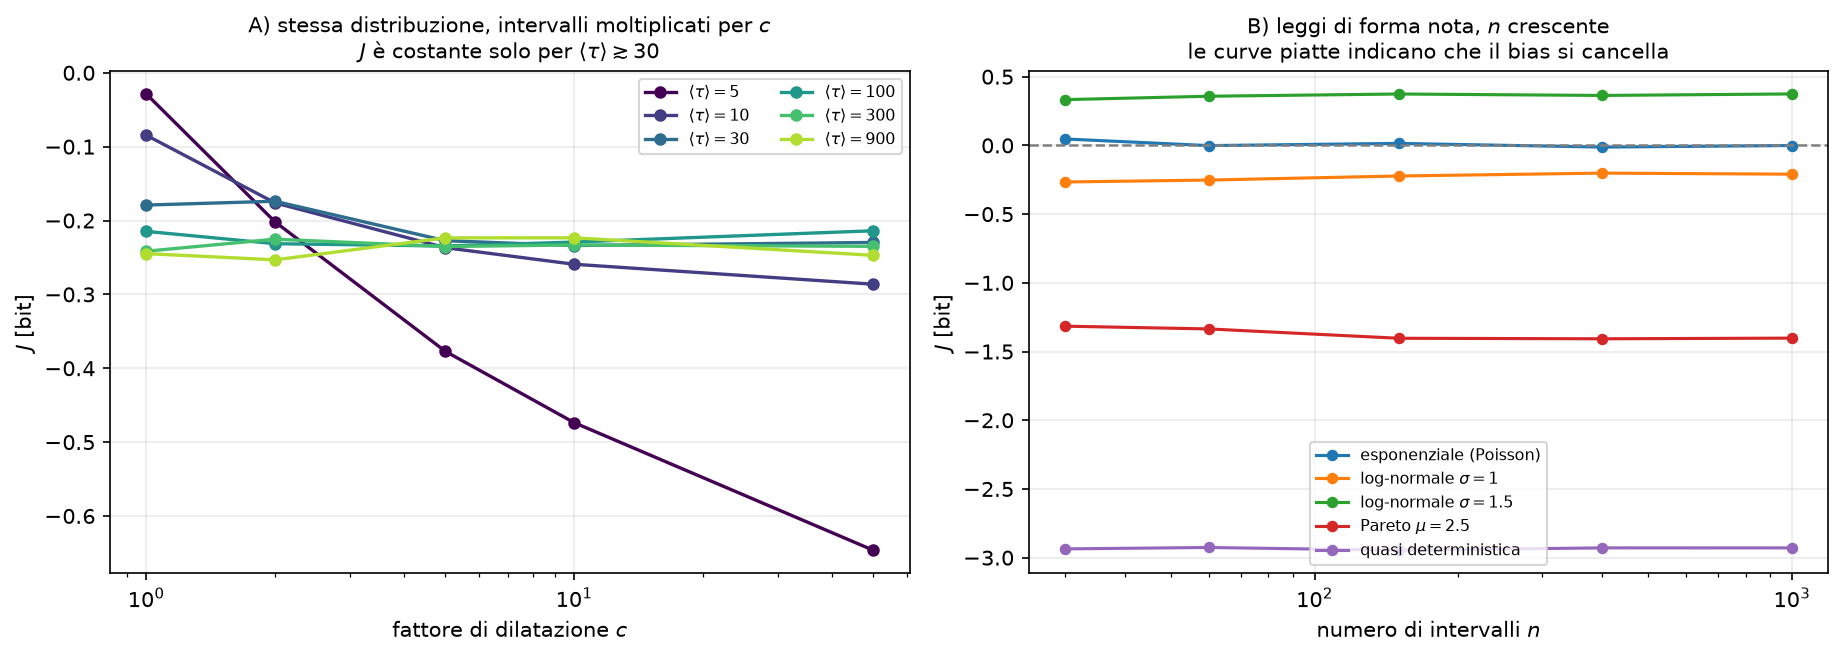
\includegraphics[width=\textwidth]{figure/cap2_invarianza_J.png}
  \caption{Limiti di validità della~\eqref{eq:entropia-intervalli}, misurati
  sullo stimatore effettivamente impiegato. A: intervalli estratti da una stessa
  legge log-normale e moltiplicati per un fattore $c$, per sei valori
  dell'intervallo medio di partenza; una curva piatta indica invarianza. Sotto
  $\langle\tau\rangle \simeq 30$ la quantizzazione agli interi la distrugge. B:
  $J$ su cinque leggi di forma nota al crescere del numero di intervalli; lo
  scostamento fra gli estremi quantifica il bias che la sottrazione del termine
  poissoniano non elimina.}
  \label{fig:invarianza-J}
\end{figure}

Valori positivi di $J$ indicano intervalli distribuiti in modo più irregolare di
un processo di Poisson, valori negativi una regolarità superiore a quella del
caso. La quantità non compare in nessuno dei lavori di riferimento ed è
introdotta qui; il §\ref{sec:entropia-intervalli} ne verifica la stabilità
rispetto alla lunghezza di analisi e la impiega per neutralizzare l'effetto
appena descritto.


% ---------------------------------------------------------------------
\section{Entropia e compressione}
\label{sec:entropia}

Il concetto di disordine di un testo e la nozione di entropia sono già stati
introdotti nel Capitolo~\ref{cap:introduzione}. Trattandosi di un concetto
centrale per questo lavoro, in questa sezione viene definito in modo formale e
ne viene esplicitato il legame con gli algoritmi di compressione, che è lo
strumento con cui l'entropia verrà effettivamente stimata sui testi.

% ---------------------------------------------------------------------
\subsection{Entropia e predicibilità}
\label{sec:entropia-def}

Si consideri una sorgente che emette simboli da un alfabeto finito
$\mathcal{X}$. Per una singola variabile aleatoria $X$ che assume il valore
$x \in \mathcal{X}$ con probabilità $p(x)$, l'entropia di
Shannon~\cite{shannon1948} è
\begin{equation}
  H(X) \;=\; -\sum_{x \in \mathcal{X}} p(x) \log_2 p(x),
  \label{eq:H-singola}
\end{equation}
espressa in bit, e misura l'incertezza media sull'esito dell'estrazione.

I simboli di un testo non sono però indipendenti, e l'entropia di una singola
lettera non descrive la sorgente: sapere che in inglese la lettera più frequente
è \emph{e} dice poco, mentre sapere che dopo \emph{th} segue quasi sempre
\emph{e} dice molto. Occorre quindi considerare blocchi di simboli. Detta
$H(X_1,\dots,X_n)$ l'entropia congiunta di un blocco di lunghezza $n$, definita
dalla~\eqref{eq:H-singola} applicata alla distribuzione congiunta dei blocchi, si
definisce il tasso di entropia della sorgente come
\begin{equation}
  h \;=\; \lim_{n\to\infty} \frac{H(X_1,\dots,X_n)}{n} .
  \label{eq:tasso-entropia}
\end{equation}
Il limite esiste per sorgenti stazionarie ed ergodiche~\cite{cover2006} e
quantifica l'incertezza media per simbolo una volta tenuto conto di tutte le
dipendenze, comprese quelle a lunga distanza. È questa, e non
la~\eqref{eq:H-singola}, la quantità pertinente per un testo.

Il teorema della codifica di sorgente~\cite{cover2006} lega $h$ alla
comprimibilità: il tasso di entropia è un limite inferiore alla lunghezza media
per simbolo di qualunque codifica senza perdita. Stimare l'entropia di un testo
e stimarne la comprimibilità sono quindi, entro le approssimazioni del caso, lo
stesso problema.

Il legame si comprende in modo intuitivo tornando ai casi limite della
Tabella~\ref{tab:tre-regimi}. Un algoritmo di compressione senza perdita opera
sostituendo alle porzioni di testo che si ripetono un riferimento
all'occorrenza precedente, più breve del testo che rimpiazza. Nel testo monotono
il medesimo gruppo di parole ricorre per l'intera lunghezza del documento: dopo
la prima occorrenza tutto il resto è un riferimento, il file compresso è
minuscolo e il tasso di entropia è prossimo a zero, perché il simbolo successivo
è quasi sempre determinato da quelli che lo precedono. Nella sequenza casuale,
al contrario, nessuna porzione si ripete: non esiste nulla cui fare riferimento,
il compressore non guadagna nulla e il tasso di entropia è massimo, perché ogni
simbolo è imprevedibile a partire dai precedenti. Il linguaggio naturale si
colloca fra i due estremi, e la quantità di compressione che ammette è una
misura diretta di quanta struttura possiede.

\paragraph{Stimatori di Lempel--Ziv.}
La stima diretta di $h$ dalla~\eqref{eq:tasso-entropia} per conteggio di blocchi
è impraticabile: il numero di blocchi distinti di lunghezza $n$ cresce
esponenzialmente con $n$, e la dimensione campionaria necessaria a stimarne le
probabilità cresce di conseguenza. Nessun testo reale è abbastanza lungo.

Si ricorre allora agli stimatori della famiglia Lempel--Ziv~\cite{ziv1977},
che aggirano il problema misurando le ripetizioni invece delle probabilità.
L'idea è la seguente: si scorre la successione e, a ogni posizione $i$, si cerca
la più lunga sottostringa che inizi in $i$ e sia già comparsa in precedenza,
detta $\Lambda_i$ la sua lunghezza. In un testo molto ripetitivo i match sono
lunghi, in un testo casuale sono corti. Si dimostra che, per una sorgente
stazionaria ed ergodica, la lunghezza media di tali match cresce come il
logaritmo della finestra esplorata e che
\begin{equation}
  h \;=\; \lim_{n\to\infty}
  \left\langle \frac{\log_2 n}{\Lambda_i} \right\rangle ,
  \label{eq:lz-entropia}
\end{equation}
dove la media è presa sulle posizioni $i$. La~\eqref{eq:lz-entropia} converge
assai più rapidamente del conteggio di blocchi e mantiene buone proprietà anche
in presenza di correlazioni a lungo raggio, che è la ragione per cui viene
adottata qui: le sorgenti considerate in questa tesi hanno, per costruzione,
memoria lunga.

% ---------------------------------------------------------------------
\subsection{Stima della cross-entropia e della divergenza}
\label{sec:crossparsing}

Le quantità introdotte finora descrivono un testo singolo. Per confrontare due
testi occorre la cross-entropia, che misura il costo di codificare un testo
usando la statistica di un altro.

L'algoritmo di cross-parsing di Ziv e Merhav~\cite{ziv1993} estende
la~\eqref{eq:lz-entropia} a due successioni. Data la successione $x$ da
misurare e la successione di riferimento $y$, si scorre $x$ da sinistra a destra
e la si decompone in frasi successive, dove ogni frase è la più lunga
sottostringa che, a partire dalla posizione corrente, compaia da qualche parte
in $y$; raggiunto il punto in cui il match si interrompe, si chiude la frase e
se ne apre una nuova. Il numero di frasi così ottenute viene indicato con
$c(x|y)$ ed è la quantità che misura la somiglianza fra i due testi: se $x$ e
$y$ provengono dalla stessa sorgente, le frasi sono lunghe e poche; se
provengono da sorgenti diverse, i match si interrompono presto e le frasi sono
molte. La stima della cross-entropia è
\begin{equation}
  h(x \,|\, y) \;=\; \frac{c(x|y)\,\log_2 |y|}{|x|},
  \label{eq:crossparsing}
\end{equation}
espressa in bit per simbolo, dove $|x|$ e $|y|$ sono le lunghezze delle due
successioni.

La divergenza di Kullback--Leibler è lo strumento con cui si quantifica quanto
due distribuzioni di probabilità differiscano fra loro. Date due distribuzioni
$P$ e $Q$ sullo stesso alfabeto, essa è definita come
\begin{equation}
  D(P\|Q) \;=\; \sum_{x} P(x) \log_2 \frac{P(x)}{Q(x)}
  \;=\; H_P(Q) - H(P),
  \label{eq:kl-def}
\end{equation}
dove $H_P(Q)$ è la cross-entropia fra le due distribuzioni. La~\eqref{eq:kl-def}
si interpreta come il numero medio di bit sprecati per simbolo codificando una
sorgente $P$ con un codice ottimizzato per $Q$: vale zero se e solo se
$P = Q$ ed è positiva altrimenti.

In termini di successioni, la~\eqref{eq:kl-def} si stima come differenza fra due
cross-entropie: dividendo $x$ in due metà $x_1$ e $x_2$ e prendendo da $y$ un
prefisso $y_1$ della stessa lunghezza di $x_1$, si pone
\begin{equation}
  D(x \,\|\, y) \;=\; h(x_2 \,|\, y_1) \;-\; h(x_2 \,|\, x_1) .
  \label{eq:kl}
\end{equation}
La seconda metà di $x$ viene cioè codificata due volte, una volta usando come
riferimento un testo estraneo e una volta usando la prima metà di $x$ stesso, e
si misura quanto costa in più la prima operazione.

L'appaiamento delle lunghezze dei due riferimenti non è un dettaglio.
La~\eqref{eq:crossparsing} dipende dalla lunghezza del riferimento, poiché un
riferimento più lungo contiene più sottostringhe e produce una cross-entropia
minore a parità di sorgente. Se i due termini della~\eqref{eq:kl} usassero
riferimenti di lunghezza diversa, la differenza conterrebbe un termine spurio
che può superare in modulo il segnale da misurare e produrre stime negative,
impossibili per la~\eqref{eq:kl-def}. Con $|y_1| = |x_1|$ il termine spurio si
cancella, e la costruzione soddisfa la proprietà verificabile $D(x\|x) = 0$
esattamente, impiegata nei capitoli sperimentali come test dello stimatore.

Poiché la~\eqref{eq:kl} non è simmetrica, mentre per confrontare due corpora
serve una quantità che non dipenda da quale dei due venga posto come
riferimento, seguendo~\cite{lippi2019} viene adottata la divergenza
simmetrizzata
\begin{equation}
  D_s(x,y) \;=\; \tfrac{1}{2}\bigl[D(x\|y) + D(y\|x)\bigr].
  \label{eq:kl-sym}
\end{equation}

% ---------------------------------------------------------------------
\subsection{Misure basate su compressione}
\label{sec:compressione}

Le stime della sottosezione precedente usano la compressione come strumento
teorico, attraverso il conteggio delle frasi. Un secondo gruppo di misure,
introdotto in questo contesto da Hadad et al.~\cite{hadad2026}, impiega invece
direttamente un compressore reale come sonda della regolarità strutturale, senza
passare per una stima di entropia.

Detta $C(x)$ la dimensione in byte del testo $x$ dopo la compressione, si
definisce il rapporto di compressione
\begin{equation}
  R_{\mathrm{gzip}}(x) \;=\; \frac{C(x)}{|x|},
  \label{eq:cratio}
\end{equation}
tanto minore quanto più il testo è regolare. Il pedice ricorda l'algoritmo
impiegato e distingue la quantità dal descrittore $R$ della~\eqref{eq:R}.

Da esso derivano la compressione condizionata
$\bigl(C(x+y) - C(x)\bigr)/|y|$, dove $x+y$ indica la concatenazione, che stima
il costo incrementale di codificare la seconda metà di un documento dopo aver
già codificato la prima e misura quindi quanto la seconda metà sia prevedibile
a partire dalla prima; e la distanza normalizzata di compressione~\cite{li2004}
\begin{equation}
  \mathrm{NCD}(x,y) \;=\;
  \frac{C(xy) - \min\{C(x),C(y)\}}{\max\{C(x),C(y)\}} .
  \label{eq:ncd}
\end{equation}
Applicata fra un testo e una sua permutazione, la~\eqref{eq:ncd} misura quanta
parte della comprimibilità dipenda dall'ordine delle parole e non dalla sola
composizione lessicale: è quindi l'analogo, in chiave di compressione, del
confronto fra i pannelli della Figura~\ref{fig:barcode}.


% ---------------------------------------------------------------------
\section{Token ed embedding}
\label{sec:token}

Nel §\ref{sec:scala} si è assunta la parola come unità fondamentale del testo,
in quanto più piccola porzione dotata di significato autonomo per un lettore
umano. Questa scelta non vale più per gli algoritmi di generazione automatica
del testo e, in particolare, per i modelli linguistici di grandi dimensioni.

Si riprenda la frase già usata come esempio,
\emph{Se pensi di comprendere la meccanica quantistica, non comprendi la
meccanica quantistica.} Per un lettore umano essa si scompone come nella
Figura~\ref{fig:scomp-parole}: dodici parole più la punteggiatura, ciascuna
delle quali ha un significato che si può cercare in un dizionario.

\begin{figure}[htbp]
  \centering
  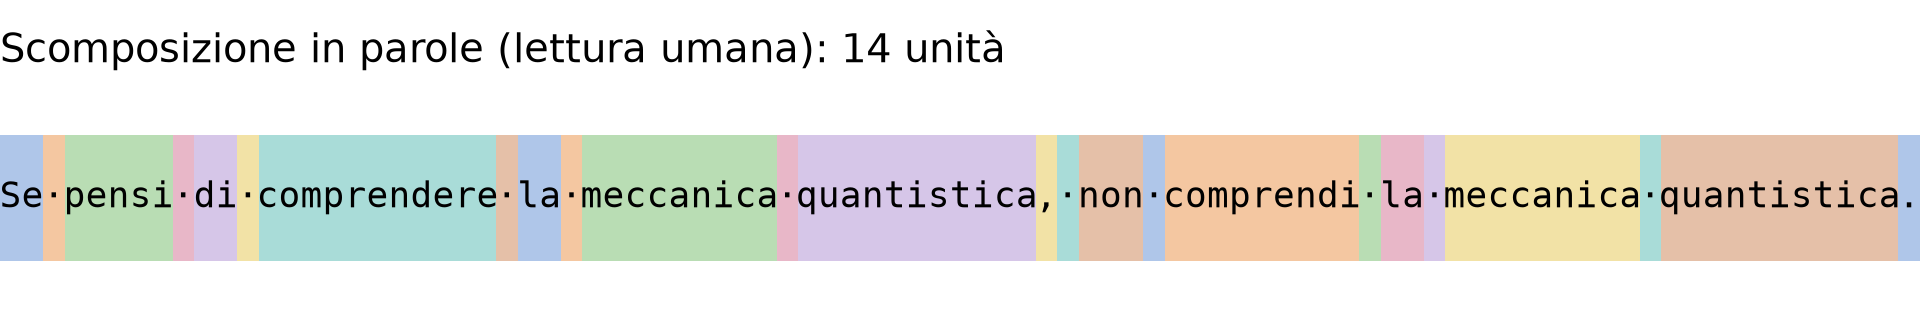
\includegraphics[width=\textwidth]{figure/cap2_scomposizione_parole.png}
  \caption{Scomposizione in parole. Ogni blocco è un'unità dotata di
  significato autonomo; il punto mediano segnala gli spazi.}
  \label{fig:scomp-parole}
\end{figure}

Per un modello linguistico la stessa frase si scompone invece come nella
Figura~\ref{fig:scomp-token}.

\begin{figure}[htbp]
  \centering
  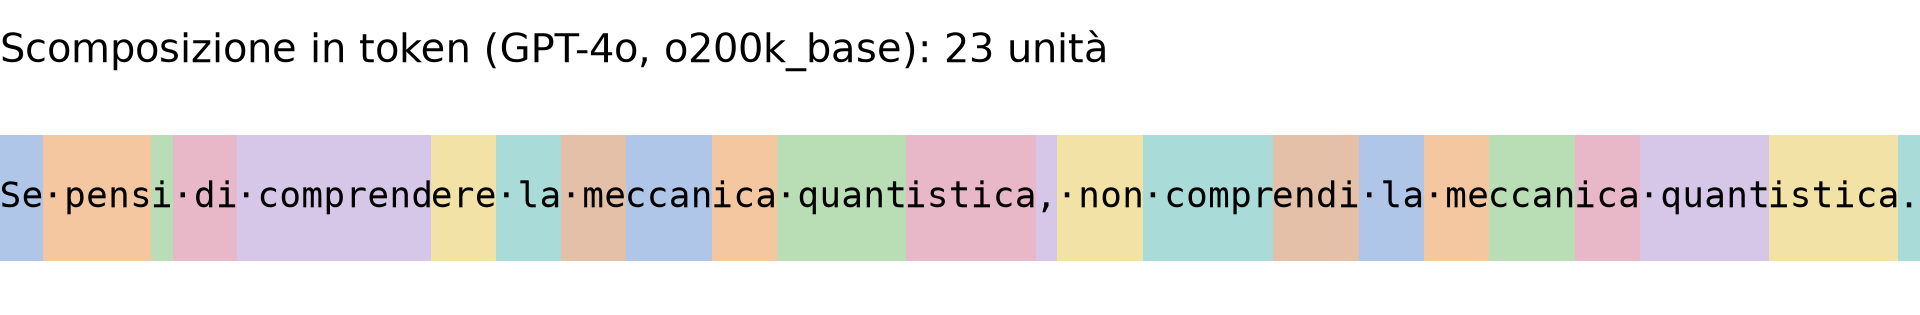
\includegraphics[width=\textwidth]{figure/cap2_scomposizione_token.png}
  \caption{Scomposizione in token della stessa frase, ottenuta con il
  tokenizzatore \texttt{o200k\_base} impiegato da GPT-4o. Le unità sono
  ventitré, non coincidono con le parole e in generale non hanno significato
  autonomo.}
  \label{fig:scomp-token}
\end{figure}

La frase non è divisa né in lettere né in parole, ma in gruppi di lettere
chiamati \emph{token}. Alcuni token coincidono con parole intere
(\texttt{·la}, \texttt{·non}), altri sono frammenti privi di significato
(\texttt{ccan}, \texttt{istica}). Si osservi in particolare la coppia
\emph{comprendere} e \emph{comprendi}: la prima si scompone in
\texttt{·comprend} e \texttt{ere}, la seconda in \texttt{·compr} e
\texttt{endi}. Due forme della stessa radice vengono dunque tagliate in punti
diversi, e il modello non riceve alcuna indicazione esplicita del fatto che
condividano la radice. Lo spazio, inoltre, non separa i token ma vi è
incorporato: la maggior parte dei token inizia con uno spazio, e la
segmentazione del testo in unità precede logicamente qualunque nozione di
parola.

La conversione avviene tramite un algoritmo detto \emph{tokenizzatore}, che
traduce un testo scritto in una qualsiasi lingua e in un qualsiasi alfabeto in
una sequenza di token estratti da un dizionario ampio ma finito, costruito una
volta per tutte a partire da un grande corpus. I dizionari dei tokenizzatori
più diffusi hanno dimensioni dell'ordine di $10^5$ elementi: quello di GPT-4o,
\texttt{o200k\_base}, ne conta \num{200019}; \texttt{cl100k\_base}, impiegato
come unità di analisi nei capitoli sperimentali per le ragioni discusse nel
Capitolo~\ref{cap:metodi}, ne conta \num{100277}; i modelli Qwen2.5 analizzati
in questa tesi ne condividono uno di circa \num{151000} voci. Poiché il
dizionario è finito ma le lingue possibili sono molte, i testi nelle lingue
meno rappresentate nel corpus di costruzione vengono frammentati in un numero
di token assai maggiore rispetto all'inglese.

Proprio come le parole per gli esseri umani, per un modello linguistico sono i
token a trasportare significato. Il significato non è però un'etichetta
associata al token, bensì una posizione: tramite un'operazione detta
\emph{embedding} ogni token viene mappato in un vettore di uno spazio a molte
dimensioni, e la geometria di quello spazio codifica le relazioni fra i token.
Vettori vicini corrispondono a token che compaiono in contesti simili, e
direzioni ricorrenti nello spazio corrispondono a relazioni ricorrenti nel
linguaggio.

La Figura~\ref{fig:embedding} mostra la proprietà su un caso concreto. I vettori
di trenta parole inglesi, appartenenti a cinque famiglie semantiche, sono
proiettati sulle prime due componenti principali dello spazio: le parole di
ciascuna famiglia si dispongono in gruppi distinti, benché la costruzione dei
vettori non abbia mai fatto uso di alcuna classificazione semantica, ma soltanto
delle co-occorrenze osservate in un corpus.

\begin{figure}[htbp]
  \centering
  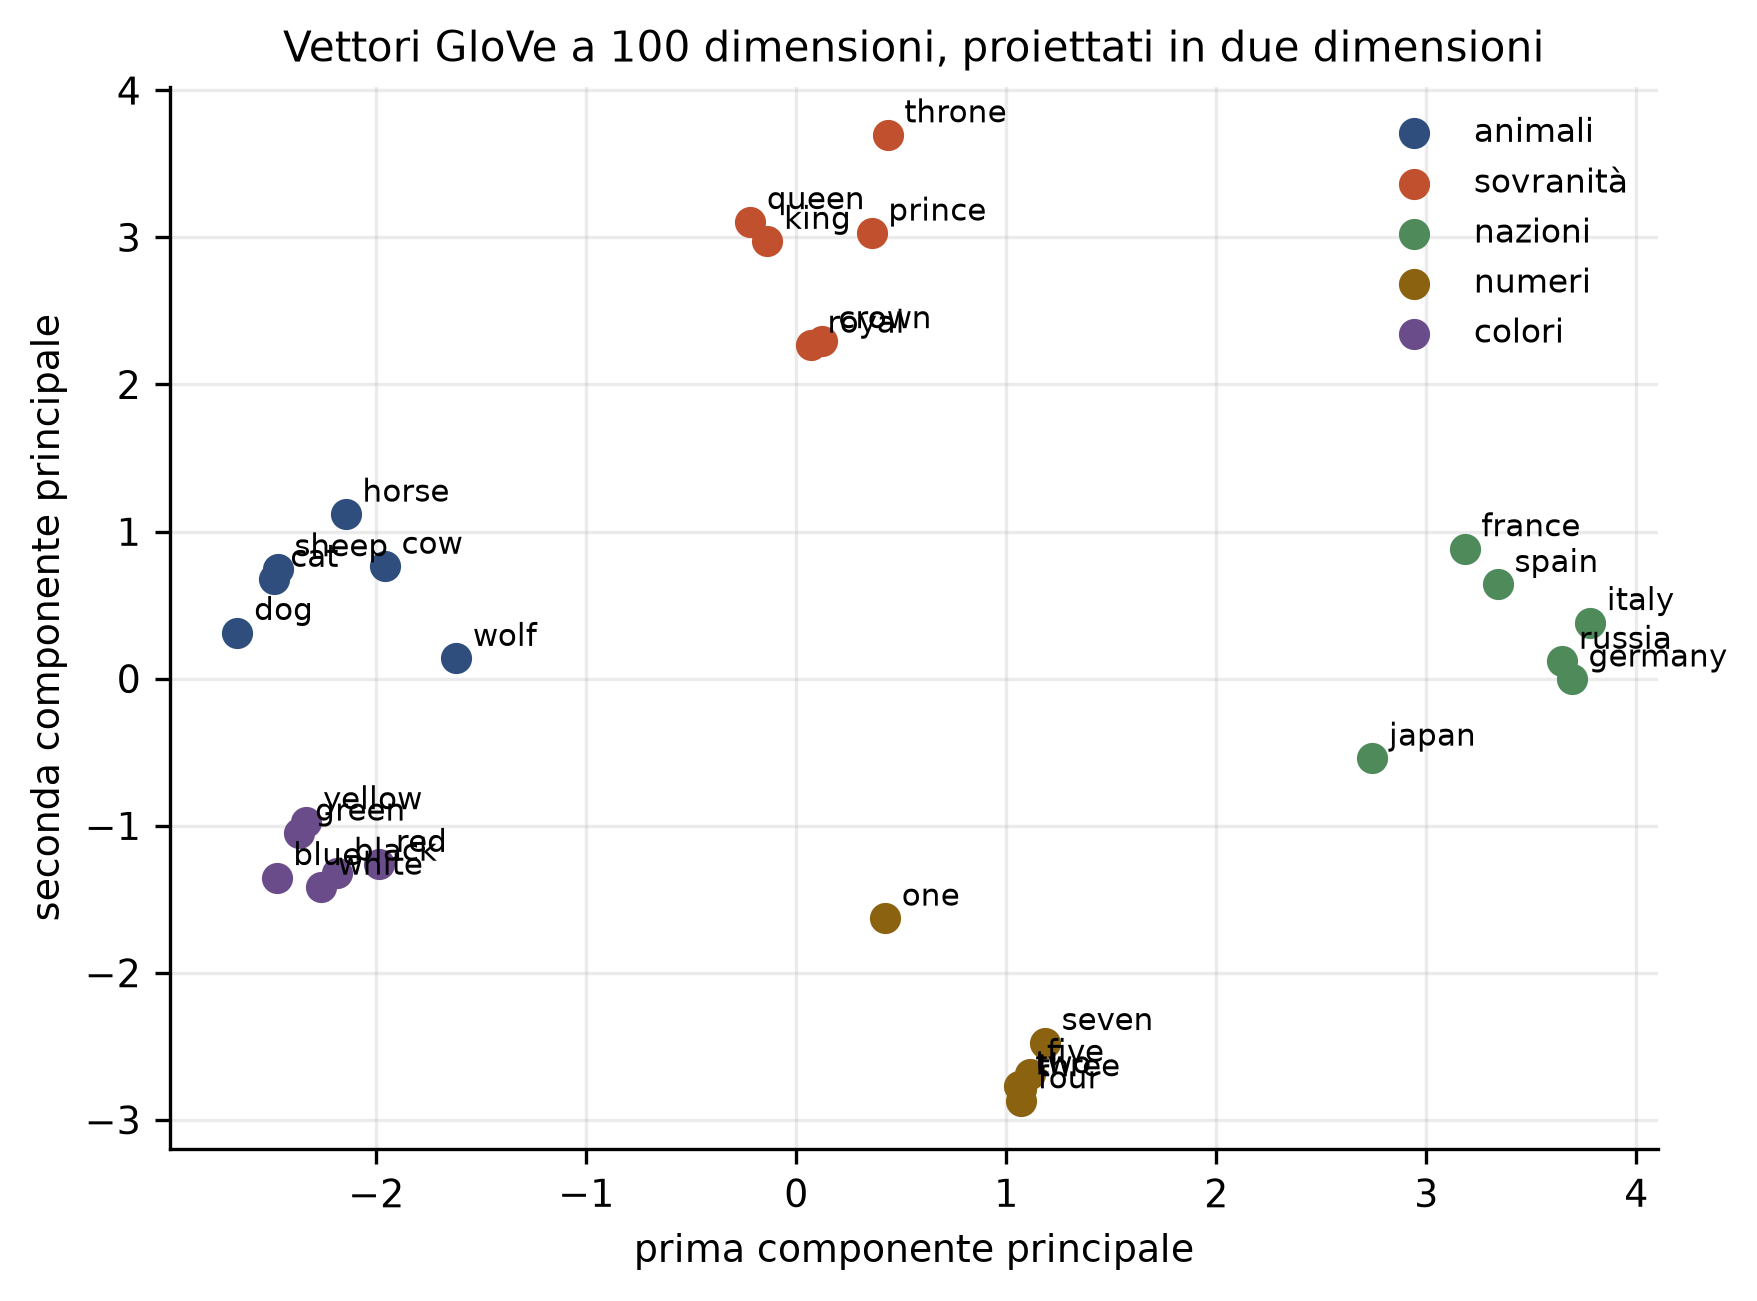
\includegraphics[width=0.82\textwidth]{figure/cap2_embedding_2d.png}
  \caption{Trenta parole inglesi rappresentate dai rispettivi vettori GloVe a
  100 dimensioni, proiettati sulle prime due componenti principali. Le cinque
  famiglie semantiche formano gruppi separati senza che alcuna informazione
  semantica sia stata fornita all'algoritmo. La proiezione conserva soltanto una
  parte della struttura, poiché riduce cento dimensioni a due: la vicinanza
  visibile in figura è una condizione sufficiente, non necessaria, alla
  vicinanza nello spazio originario.}
  \label{fig:embedding}
\end{figure}

I due spazi vettoriali che compaiono in questo lavoro hanno natura diversa. Ogni modello linguistico possiede una propria matrice di embedding,
appresa durante l'addestramento insieme a tutti gli altri parametri, e i cui
vettori non sono direttamente confrontabili fra modelli diversi: fra i modelli
analizzati in questa tesi la dimensione di tale spazio passa da 1536 per il
modello da 1.5 miliardi di parametri a 5120 per quello da 14 miliardi. Gli embedding impiegati nelle analisi di
questa tesi sono invece vettori GloVe a 100 dimensioni, pre-addestrati su un
corpus esterno e identici per tutti i testi esaminati: la scelta è dettata dalla
necessità di misurare i testi generati da modelli diversi con lo stesso metro, e
segue l'impostazione di~\cite{mikhaylovskiy2025states}. Nel
§\ref{sec:traiettoria} tali vettori verranno usati per trasformare un testo in
una traiettoria nello spazio semantico e studiarne l'autocorrelazione.


% ---------------------------------------------------------------------
\section{Generazione autoregressiva e temperatura}
\label{sec:temperatura}

Un modello linguistico autoregressivo, data una sequenza di token $t_{1:m}$,
sceglie il token successivo estraendolo da una distribuzione di probabilità che
dipende dalla sequenza stessa. La probabilità dell'intera sequenza si
decompone per mezzo della regola della catena,
\begin{equation}
  P(t_{1:m}) \;=\; \prod_{k=1}^{m} P(t_k \mid t_{1:k-1}),
  \label{eq:autoregressivo}
\end{equation}
e il modello è addestrato ad approssimare i singoli fattori
$P(t_k \mid t_{1:k-1})$, cioè a prevedere ogni token a partire da tutti quelli
che lo precedono. La generazione consiste nell'applicare ripetutamente questa
previsione, aggiungendo di volta in volta il token estratto alla sequenza che
condiziona l'estrazione successiva.

\paragraph{Origine della distribuzione condizionata.}
Il modo in cui il modello costruisce $P(t_k \mid t_{1:k-1})$ è ciò che
distingue le architetture moderne da quelle precedenti, ed è rilevante per
questo lavoro. I modelli oggi in uso si basano sull'architettura
\emph{transformer}~\cite{vaswani2017}, il cui elemento caratteristico è il
meccanismo di \emph{attenzione}. In esso ogni posizione della sequenza calcola
un peso per ciascuna delle posizioni precedenti e costruisce la propria
rappresentazione come combinazione pesata di quelle: il token in posizione $k$
può quindi attingere direttamente a qualunque token precedente, per lontano che
sia, senza che l'informazione debba propagarsi attraverso le posizioni
intermedie.

È una differenza sostanziale rispetto ai modelli ricorrenti, in cui
l'informazione proveniente da una posizione lontana deve attraversare tutte
quelle interposte e si degrada di conseguenza. Nel transformer il cammino fra
due posizioni qualsiasi ha lunghezza costante, e questo rende l'architettura in
linea di principio capace di rappresentare dipendenze fra porzioni di testo
molto distanti fra loro. È il meccanismo che, negli attuali modelli, potrebbe
dare origine alle correlazioni a lungo raggio descritte nel §\ref{sec:lrc}, e
una delle ragioni per cui ha senso cercarle nel testo generato. La capacità di
rappresentare tali dipendenze non implica però che il modello le riproduca
effettivamente, e l'attenzione opera comunque entro una finestra di contesto
finita: stabilire se le correlazioni siano presenti nel
testo prodotto resta una questione empirica, ed è precisamente quella affrontata
nei capitoli sperimentali.

\paragraph{Temperatura.}
Il modello non produce direttamente probabilità, ma valori reali detti
\emph{logit}, indicati con $u_1,\dots,u_{|\mathcal{L}|}$, uno per ciascun
elemento del dizionario $\mathcal{L}$. Essi vengono convertiti in distribuzione
di probabilità da una funzione softmax riscalata da un parametro
$T$~\cite{ackley1985}:
\begin{equation}
  p(t = \mathcal{L}_l \mid t_{1:i-1}) \;=\;
  \frac{\exp(u_l / T)}{\sum_{l'} \exp(u_{l'} / T)} .
  \label{eq:softmax}
\end{equation}

Il parametro $T$ prende il nome di temperatura, e la denominazione non è una
semplice analogia. Ponendo $E_l = -u_l$, la~\eqref{eq:softmax} coincide con la
distribuzione di Boltzmann $p_l \propto e^{-E_l/T}$ di un sistema a
$|\mathcal{L}|$ stati in equilibrio termico alla temperatura $T$. Questa
identificazione è ciò che giustifica la ricerca, nel testo generato, dei
fenomeni caratteristici dei sistemi termodinamici, e in particolare delle
transizioni di fase discusse nel §\ref{sec:fasi}.

I due limiti sono immediati. Per $T\to0$ la distribuzione si concentra sul token
di logit massimo e la generazione diventa deterministica; per $T\to\infty$ tende
alla distribuzione uniforme sull'intero dizionario, indipendentemente dal
contesto. Fra i due estremi, valori $T<1$ concentrano la massa di probabilità
sugli eventi più probabili, mentre valori $T>1$ la ridistribuiscono verso quelli
meno probabili. La temperatura non modifica dunque ciò che il modello ha
appreso, ma soltanto quanto fedelmente la generazione segue la distribuzione
appresa.

Nella pratica corrente la generazione impiega anche il troncamento della
distribuzione, nelle varianti top-$k$~\cite{fan2018} e
top-$p$~\cite{holtzman2020}, e penalità che scoraggiano la ripetizione. Tutti
questi meccanismi agiscono sulla stessa distribuzione e introducono un secondo
parametro d'ordine, rendendo impossibile attribuire alla sola temperatura il
comportamento osservato. Per questa ragione, e coerentemente con la scelta
esplicita di~\cite{mikhaylovskiy2025zipf}, i dati analizzati in questa tesi sono
stati generati impiegando il solo campionamento per temperatura.


% ---------------------------------------------------------------------
\section{Fasi e stato critico}
\label{sec:fasi}

Una fase di un sistema fisico è uno stato, tipicamente di equilibrio, dotato di
proprietà macroscopiche caratteristiche e stabile in una regione dello spazio
dei parametri; alla frontiera di tali regioni avviene una transizione di fase.
Secondo la classificazione di Ehrenfest~\cite{ehrenfest1933} una transizione di
ordine $n$ è una discontinuità nella derivata $n$-esima dell'energia libera.

Applicare alla lettera questa classificazione al testo generato non è però
possibile. Il sistema considerato non ha un'energia libera di cui prendere
derivate, non è in equilibrio con alcun bagno termico e
non possiede un limite termodinamico, poiché il numero di token di un documento
resta finito. Ciò che rende legittimo il linguaggio delle fasi è la
corrispondenza stabilita nel §\ref{sec:temperatura}: la~\eqref{eq:softmax}
coincide con una distribuzione di Boltzmann in cui i logit giocano il ruolo di
energie e il parametro di campionamento quello di temperatura. La distribuzione
condizionata da cui ogni token viene estratto è dunque, letteralmente, una
distribuzione di Gibbs, e $T$ ne è la temperatura. Quello che resta analogia, e
non identità, è il passaggio dal singolo token al documento: nulla garantisce
che le proprietà collettive di una sequenza generata token per token si
comportino come le proprietà macroscopiche di un sistema all'equilibrio. Il
vocabolario di Ehrenfest viene perciò impiegato in senso descrittivo, per
nominare regioni di comportamento qualitativamente diverso separate da
variazioni rapide, e non per rivendicare una transizione di fase in senso
termodinamico.

Ciò che rende il concetto utile è il comportamento nel punto critico che
separa due fasi: là le correlazioni decadono a legge di potenza e la loro
portata diverge, e molte grandezze osservabili esibiscono lo stesso andamento.
Il criterio inverso, per cui dove compare una legge di potenza si sospetta uno
stato critico, va maneggiato con prudenza, perché distribuzioni a legge di
potenza si generano in molti modi che con la criticità non hanno rapporto, dal
semplice prodotto di variabili aleatorie ai processi di preferential
attachment. Preso da solo, l'andamento a legge di potenza di una quantità non
dimostra nulla. Acquista forza quando più osservabili indipendenti cambiano
regime allo stesso valore del parametro di controllo, ed è in questa forma che
viene impiegato nel §\ref{sec:tstar}: non la legge di potenza di una misura,
ma la convergenza di criteri costruiti per scopi diversi.

Il quadro è stato applicato ai modelli linguistici in~\cite{nakaishi2024}, dove
la temperatura di campionamento separa una fase a bassa temperatura,
caratterizzata da strutture ripetitive, da una ad alta temperatura in cui il
testo è incomprensibile. La tesi sostenuta in quel lavoro è che il linguaggio
naturale si collochi \emph{sul} punto critico fra le due: nello spazio dei
processi stocastici che generano successioni di simboli, il processo
corrispondente a una lingua naturale giacerebbe sulla superficie critica che
separa le due regioni, e un modello addestrato su quella lingua definisce una
famiglia di processi che quella superficie attraversa al variare di $T$. Il
risultato è verificato su modelli da 160 milioni a 2.8 miliardi di parametri, su
sei lingue e su due diverse mappature del testo in successione numerica, il che
ne stabilisce l'indipendenza dalla scala e dalla lingua.

Questa congettura è il punto di contatto più stretto fra il presente lavoro e la
letteratura di fisica statistica sull'argomento, e il
Capitolo~\ref{cap:risultati1} ne fornisce una verifica indipendente: se il
linguaggio naturale è critico, allora la temperatura alla quale il testo
generato somiglia di più a quello umano deve coincidere con quella alla quale il
modello attraversa la transizione, e criteri che misurano proprietà diverse
devono indicarla concordemente.


% ---------------------------------------------------------------------
\subsection{La traiettoria di embedding}
\label{sec:traiettoria}

Il §\ref{sec:token} ha introdotto i vettori di embedding come rappresentazione
del significato. Applicandoli a un testo si ottiene un oggetto geometrico: detta
$(p_1,\dots,p_M)$ la successione delle parole del documento e $v(\cdot)$ la
mappa che associa a una parola il proprio vettore, si pone
\begin{equation}
  \mathbf{m}_i \;=\;
  \begin{cases}
    v(p_i) - \bar{v} & \text{se $p_i$ ha un vettore},\\[2pt]
    \mathbf{0}       & \text{altrimenti},
  \end{cases}
  \label{eq:traiettoria}
\end{equation}
dove $\bar{v}$ è la media dei vettori delle sole parole che ne possiedono uno.
La successione $(\mathbf{m}_1,\dots,\mathbf{m}_M)$ è la traiettoria del testo
nello spazio degli embedding: ogni parola è un punto, e leggere il documento
dall'inizio alla fine equivale a percorrere quella traiettoria.

Due dettagli della~\eqref{eq:traiettoria} incidono sui risultati. Il primo è la
centratura: sottrarre $\bar{v}$ elimina la
direzione media del documento, che altrimenti dominerebbe ogni prodotto scalare
e renderebbe tutte le coppie di parole artificialmente simili. Il secondo è il
trattamento delle parole prive di vettore, alle quali si assegna il vettore
nullo \emph{dopo} la centratura, seguendo~\cite{mikhaylovskiy2025states}: la
posizione nella successione viene così conservata, e con essa la struttura dei
lag, ma la parola non contribuisce ad alcuna correlazione. La conseguenza è che
un testo in cui molte parole non hanno vettore produce una traiettoria fatta in
larga parte di zeri, e le misure che seguono perdono significato prima di
diventare incalcolabili: è la ragione della soglia di validità introdotta più
avanti.

Su questa successione si definisce l'autocorrelazione a distanza $\tau$ come
media della similarità coseno fra i vettori che distano $\tau$ posizioni,
\begin{equation}
  C(\tau) \;=\; \frac{1}{M-\tau} \sum_{i=1}^{M-\tau}
  \frac{\mathbf{m}_i \cdot \mathbf{m}_{i+\tau}}
       {\lVert \mathbf{m}_i \rVert \, \lVert \mathbf{m}_{i+\tau} \rVert},
  \label{eq:acf-embedding}
\end{equation}
con la convenzione che i termini in cui uno dei due vettori è nullo
contribuiscono zero. La~\eqref{eq:acf-embedding} risponde alla domanda: due
parole che distano $\tau$ posizioni tendono a essere semanticamente affini? Vale
$C(\tau) \simeq 0$ quando non c'è alcuna relazione, ed è tanto più vicina a uno
quanto più il testo, a quella distanza, torna a parlare della stessa cosa.

Poiché la~\eqref{eq:acf-embedding} resta calcolabile su qualunque successione,
serve un riferimento che dica quale ampiezza sia distinguibile dal caso. Si
adotta il rimescolamento: si permutano a caso le posizioni della traiettoria, si
ricalcola $C(\tau)$ e si prende il massimo del suo modulo. Il valore così
ottenuto è il livello di rumore del documento, ed è la stessa costruzione dei
null model del §\ref{sec:null}: conserva il contenuto e distrugge l'ordine.
Un'autocorrelazione la cui ampiezza non superi quel livello non è distinguibile
da una successione di parole senza struttura.


% ---------------------------------------------------------------------
\subsection{Le tre fasi}
\label{sec:tre-fasi}

Applicando questo linguaggio al testo generato,
in~\cite{mikhaylovskiy2025states} vengono individuate tre fasi, distinte dal
comportamento di $C(\tau)$.

A bassa temperatura il testo degenera in cicli di ripetizione: la traiettoria
ripassa periodicamente per gli stessi punti, $C(\tau)$ oscilla con periodo pari
alla lunghezza del ciclo e la sua trasformata di Fourier presenta picchi netti.
La quantità che segnala il fenomeno è quindi
\begin{equation}
  \Phi \;=\; \max_{k \ge 1} \bigl\lvert \hat{C}_k \bigr\rvert ,
  \label{eq:periodicita}
\end{equation}
dove $\hat{C}_k$ sono i coefficienti della trasformata discreta di $C(\tau)$. Il
coefficiente $k = 0$ viene escluso perché proporzionale alla media di $C(\tau)$,
cioè al livello complessivo di correlazione e non alla sua periodicità: un testo
uniformemente correlato ma non ciclico ha $\hat{C}_0$ grande e tutti gli altri
coefficienti piccoli. Questa è la fase che, per analogia con gli stati della
materia, viene detta solida. È lo stesso regime in cui, come osservato nel
§\ref{sec:ponte}, la fluttuazione della DFA satura e $\alpha_{\mathrm{DFA}}$
scende verso zero: le due misure segnalano lo stesso fenomeno da due angolazioni
diverse.

La~\eqref{eq:periodicita} si comporta come un parametro d'ordine nel senso che
assume valori grandi in una fase e piccoli nell'altra, ma non si annulla
identicamente fuori dalla fase periodica: su una successione priva di struttura
resta un valore residuo dovuto alle fluttuazioni campionarie. Il
Capitolo~\ref{cap:risultati1} riporta di conseguenza il suo crollo in termini di
ordini di grandezza e non di annullamento.

In una finestra ristretta di temperature $C(\tau)$ decade invece a legge di
potenza: è lo stato critico, quello in cui le leggi di Zipf e di Heaps
introdotte nel §\ref{sec:scala} risultano meglio soddisfatte. Ad alta
temperatura, infine, le correlazioni decadono esponenzialmente e non sussiste
struttura a lungo raggio: è la fase detta amorfa, o gassosa.

Per distinguere le ultime due fasi vengono confrontati due fit
dell'autocorrelazione, uno a legge di potenza e uno esponenziale, tramite il
rapporto dei rispettivi errori~\cite{mikhaylovskiy2023}:
\begin{equation}
  \mathrm{GAPELMAPER} \;=\;
  \frac{\mathrm{MAPE}\bigl(\text{fit a legge di potenza}\bigr)}
       {\mathrm{MAPE}\bigl(\text{fit esponenziale}\bigr)},
  \label{eq:gapelmaper}
\end{equation}
dove il MAPE è quello definito nella~\eqref{eq:mape}. Il rapporto è minore di 1
quando il fit a legge di potenza descrive i dati meglio di quello esponenziale,
e segnala quindi lo stato critico; è maggiore di 1 nella fase amorfa.

La~\eqref{eq:gapelmaper} è un rapporto fra errori di fit, e come tale resta
calcolabile anche quando l'autocorrelazione è indistinguibile dal rumore; in
quel regime, però, il suo valore è privo di contenuto informativo, perché
entrambi i fit descrivono male dati che non contengono alcun segnale.

Le tre fasi, la soglia di periodicità e la condizione di validità si compongono
nella regola seguente. Detti $\kappa$ la quota di parole del documento dotate di
un vettore, $A = \max_\tau \lvert C(\tau)\rvert$ l'ampiezza
dell'autocorrelazione e $\eta$ il livello di rumore stimato per rimescolamento,
un documento viene classificato come
%
\begin{itemize}
  \item \emph{non valutabile}, se $\kappa < \kappa_{\min}$ oppure $A \le \eta$;
  \item \emph{solido}, altrimenti, se $\Phi > \Phi_{\min}$;
  \item \emph{critico}, altrimenti, se $\mathrm{GAPELMAPER} < 1$;
  \item \emph{amorfo} in ogni altro caso.
\end{itemize}
%
L'ordine dei controlli non è indifferente. La condizione di validità viene per
prima perché le altre due misure, su un documento che non la supera, sono numeri
senza referente; la periodicità viene prima del GAPELMAPER perché
un'autocorrelazione periodica non è né una legge di potenza né un esponenziale,
e sottoporla a quel confronto restituirebbe un valore arbitrario. I due valori
di soglia sono fissati nel Capitolo~\ref{cap:risultati1}, dove ne vengono
discussi l'origine e l'effetto.

I due quadri di riferimento non coincidono del tutto.
In~\cite{nakaishi2024} le fasi sono due e ciò che le separa è un punto critico,
cioè un insieme di misura nulla nello spazio dei parametri;
in~\cite{mikhaylovskiy2025states} lo stato critico diventa invece una fase a sé,
dotata di estensione finita. La differenza non è terminologica: nel primo caso
attraversare la transizione con uno sweep a passo finito significa quasi
certamente saltare il punto critico, nel secondo significa attraversare una
regione che si può campionare. Il Capitolo~\ref{cap:risultati1} riporta i dati
pertinenti alla questione senza pretendere di risolverla.


% ---------------------------------------------------------------------
\section{Notazione}
\label{sec:notazione}

Le grandezze introdotte in questo capitolo provengono da lavori che adottano
simboli in conflitto fra loro. La Tabella~\ref{tab:notazione} raccoglie la
notazione seguita in questa tesi, che viene mantenuta senza eccezioni nei
capitoli successivi.

\begin{table}[htbp]
\centering
\small
\begin{tabular}{@{}l>{\raggedright\arraybackslash}p{8.3cm}c@{}}
\toprule
Simbolo & Grandezza & Definita in \\
\midrule
\multicolumn{3}{@{}l}{\itshape Testo e vocabolario} \\
$\mathbf{W}$, $w_t$, $N$ & sequenza di parole, parola in posizione $t$, lunghezza & \eqref{eq:sequenza} \\
$\mathcal{D}$, $\mathcal{D}(t)$ & dizionario e dizionario parziale & §\ref{sec:scala} \\
$f(r)$, $\alpha$ & frequenza della parola di rango $r$, esponente di Zipf & \eqref{eq:zipf} \\
$\gamma_H$ & esponente di Heaps & \eqref{eq:heaps} \\
$R$ & parole nuove nella seconda metà, rapportate alla prima & \eqref{eq:R} \\
MAPE & errore percentuale assoluto medio del fit & \eqref{eq:mape} \\
\addlinespace
\multicolumn{3}{@{}l}{\itshape Correlazioni} \\
$x_k$ & successione binaria generata da un osservabile & \eqref{eq:osservabile} \\
$c(s)$, $\theta$ & autocorrelazione a distanza $s$ e suo esponente di decadimento & \eqref{eq:acf-power} \\
$X(t)$, $\sigma_X^2$, $\gamma$ & conteggio, sua varianza, esponente di crescita & \eqref{eq:sigma} \\
$F(s)$, $\alpha_{\mathrm{DFA}}$ & fluttuazione detrendizzata e suo esponente & \eqref{eq:dfa-alpha} \\
\addlinespace
\multicolumn{3}{@{}l}{\itshape Intervalli e burstiness} \\
$\tau_i$, $p(\tau)$ & intervalli fra occorrenze e loro distribuzione & §\ref{sec:burst} \\
cv, $B$ & coefficiente di variazione, indice di Goh--Barabási & \eqref{eq:cv}, \eqref{eq:goh} \\
$S(0)$, $c_\tau(k)$ & spettro a frequenza nulla, autocorrelazione degli intervalli & \eqref{eq:eq4} \\
$\hat\gamma_{A1}$, $\hat\gamma_{A2}$ & esponenti misurati sui due null model & §\ref{sec:null} \\
$q$ & quota di burstiness & \eqref{eq:quota} \\
$\mu$, $\tau_c$ & esponente di coda e cut-off di $p(\tau)$ & \eqref{eq:troncata} \\
$J$ & entropia degli intervalli, riferita al processo di Poisson & \eqref{eq:entropia-intervalli} \\
\addlinespace
\multicolumn{3}{@{}l}{\itshape Entropia e compressione} \\
$H$, $h$ & entropia di Shannon, tasso di entropia & \eqref{eq:H-singola}, \eqref{eq:tasso-entropia} \\
$c(x|y)$, $h(x|y)$ & frasi del cross-parsing, cross-entropia stimata & \eqref{eq:crossparsing} \\
$D(x\|y)$, $D_s$ & divergenza di Kullback--Leibler e sua versione simmetrizzata & \eqref{eq:kl}, \eqref{eq:kl-sym} \\
$C(x)$, $R_{\mathrm{gzip}}$ & dimensione compressa e rapporto di compressione & \eqref{eq:cratio} \\
NCD & distanza normalizzata di compressione & \eqref{eq:ncd} \\
\addlinespace
\multicolumn{3}{@{}l}{\itshape Generazione e fasi} \\
$u_l$, $T$ & logit del token $l$, temperatura di campionamento & \eqref{eq:softmax} \\
$C(\tau)$ & autocorrelazione della traiettoria di embedding & \eqref{eq:acf-embedding} \\
$\Phi$ & parametro di periodicità di $C(\tau)$ & \eqref{eq:periodicita} \\
GAPELMAPER & rapporto fra gli errori dei due fit dell'autocorrelazione & \eqref{eq:gapelmaper} \\
$N_{\mathrm{eff}}$ & lunghezza comune di analisi & §\ref{sec:scelte} \\
\bottomrule
\end{tabular}
\caption{Notazione adottata in questa tesi.}
\label{tab:notazione}
\end{table}

Per tre simboli la scelta operata qui si discosta da quella di almeno una delle
fonti; la Tabella~\ref{tab:collisioni} riassume le corrispondenze.

\begin{center}
\small
\begin{tabular}{@{}lcccc@{}}
\toprule
Grandezza & Qui & \cite{mikhaylovskiy2025zipf} & \cite{lippi2019} & \cite{altmann2012} \\
\midrule
Esponente di Zipf                  & $\alpha$                & $\alpha$ & $\beta$  & --- \\
Esponente di Heaps                 & $\gamma_H$              & $\beta$  & $\nu$    & --- \\
Esponente della fluttuazione (DFA) & $\alpha_{\mathrm{DFA}}$ & ---      & $\alpha$ & --- \\
Decadimento dell'autocorrelazione  & $\theta$                & ---      & $\gamma$ & $\beta$ \\
Crescita della varianza del conteggio & $\gamma$             & ---      & ---      & $\gamma$ \\
Rapporto di compressione           & $R_{\mathrm{gzip}}$     & ---      & ---      & --- \\
\bottomrule
\end{tabular}
\captionof{table}{Corrispondenza fra la notazione adottata e quella delle fonti primarie,
limitatamente ai simboli per cui le fonti divergono. Il rapporto di compressione
è indicato con $R(x)$ in~\cite{hadad2026}, dove però $R$ non ha il significato
che assume qui.}
\label{tab:collisioni}
\end{center}

Il simbolo $\alpha$ è riservato all'esponente di Zipf, come
in~\cite{mikhaylovskiy2025zipf}, mentre l'esponente della detrended
fluctuation analysis, indicato con $\alpha$ in~\cite{lippi2019}, riceve il
pedice $\mathrm{DFA}$. L'esponente di Heaps è indicato con $\gamma_H$ anziché
con $\beta$ o $\nu$, per lasciare $\gamma$ libero per l'esponente di crescita
della varianza del conteggio, che è la convenzione di~\cite{altmann2012} e
della seconda parte sperimentale. Il decadimento dell'autocorrelazione riceve
infine il simbolo $\theta$, che nessuna delle fonti impiega, poiché entrambe
le lettere che gli sono attribuite in letteratura sono già assegnate. La
lettera $R$ resta al descrittore di~\cite{mikhaylovskiy2025zipf} e il rapporto
di compressione riceve il pedice $\mathrm{gzip}$.

Valgono inoltre le convenzioni seguenti, usate nel seguito senza ulteriore
avviso. Il circonflesso indica una quantità stimata dai dati in contrapposizione
al corrispondente valore teorico, come in $\hat\gamma$. I pedici $A1$ e $A2$
indicano i due null model del §\ref{sec:null}. Il simbolo $|\cdot|$ applicato a
un insieme ne indica la cardinalità e applicato a un testo la lunghezza, in
parole o in byte secondo il contesto. Le medie sono indicate con
$\langle\cdot\rangle$ e si intendono calcolate sull'intero documento salvo
diversa indicazione.

%  Le figure sono attese in figure/; la provenienza e in appendice_figure.tex
% =====================================================================

\chapter{Quadro teorico}
\label{cap:teoria}

In questo capitolo si introducono gli strumenti matematici con cui storicamente
si sono analizzati i testi e che, anche in questo lavoro, ricopriranno un ruolo
centrale: le leggi di scala del vocabolario, le misure di correlazione a lungo
raggio, la statistica degli intervalli fra occorrenze e le stime di entropia
ottenute per compressione.

Successivamente vengono introdotti gli elementi di base del funzionamento dei
modelli linguistici di grandi dimensioni, il linguaggio delle transizioni di
fase con cui alcuni risultati verranno interpretati, e la notazione adottata nel
resto della tesi.


% ---------------------------------------------------------------------
\section{Leggi di scala del vocabolario}
\label{sec:scala}

Come già anticipato, un testo può essere visto come una sequenza di simboli,
siano essi lettere, parole o, come si vedrà nel §\ref{sec:token}, token. La
scelta più naturale per un lettore umano è assumere come unità fondamentale la
parola, in quanto più piccola unità di testo dotata di significato autonomo.

Un testo è quindi una sequenza ordinata di parole
\begin{equation}
  \mathbf{W} \;=\; (w_1, w_2, \dots, w_N),
  \label{eq:sequenza}
\end{equation}
dove $N$ è la lunghezza del testo e l'indice $t = 1,\dots,N$ individua la
posizione di ciascuna parola. L'insieme delle parole distinte che vi compaiono
si dice dizionario e si indica con $\mathcal{D}$; si definisce inoltre il
dizionario parziale $\mathcal{D}(t)$ come l'insieme delle parole distinte
contenute nel prefisso $(w_1,\dots,w_t)$. Valgono per costruzione
$\mathcal{D}(N) = \mathcal{D}$ e $\mathcal{D}(t) \subseteq \mathcal{D}(t+1)$: il
dizionario parziale è una successione non decrescente di insiemi.

A titolo di esempio si consideri la frase
\begin{center}
\emph{Se pensi di comprendere la meccanica quantistica, non comprendi la
meccanica quantistica.}
\end{center}
Con la notazione introdotta si ha $N = 12$, $w_7 = \text{\emph{quantistica}}$ e
\begin{align}
  \mathcal{D}    &= \{\text{se, pensi, di, comprendere, la, meccanica,
                          quantistica, non, comprendi}\}, \\
  \mathcal{D}(6) &= \{\text{se, pensi, di, comprendere, la, meccanica}\} .
\end{align}
Il dizionario completo contiene nove parole distinte a fronte di dodici
occorrenze: le tre ripetizioni di \emph{la}, \emph{meccanica} e
\emph{quantistica} non lo accrescono.

Le due analisi più semplici che si possano condurre su $\mathbf{W}$ sono lo
studio delle frequenze delle singole parole e quello dell'andamento di
$|\mathcal{D}(t)|$ in funzione di $t$. Sono le analisi che hanno portato alla
formulazione delle due leggi empiriche enunciate nel seguito, dovute
rispettivamente a Zipf~\cite{zipf1949} e a Herdan~\cite{herdan1964} e
Heaps~\cite{heaps1978}.

% ---------------------------------------------------------------------
\subsection{Legge di Zipf}
\label{sec:zipf}

Si contino le occorrenze di ciascuna parola distinta e si ordinino le parole per
frequenza decrescente, associando a ognuna il proprio rango $r$: la parola di
rango 1 è la più frequente del testo, quella di rango 2 la seconda, e così via.
Detta $f(r)$ la frequenza della parola di rango $r$, si osserva empiricamente in
tutti i testi naturali che
\begin{equation}
  f(r) \;\propto\; r^{-\alpha}.
  \label{eq:zipf}
\end{equation}
La~\eqref{eq:zipf} prende il nome di legge di Zipf. In coordinate
bilogaritmiche corrisponde a una retta di pendenza $-\alpha$, ed è in tali
coordinate che viene di norma rappresentata e stimata.

La Figura~\ref{fig:zipf} riporta la relazione rango-frequenza per cinque romanzi
in cinque lingue diverse. Le curve sono approssimativamente rettilinee su circa
tre decadi di rango e hanno pendenze molto simili fra loro, nonostante le opere
differiscano per epoca, lingua e lunghezza.

\begin{figure}[htbp]
  \centering
  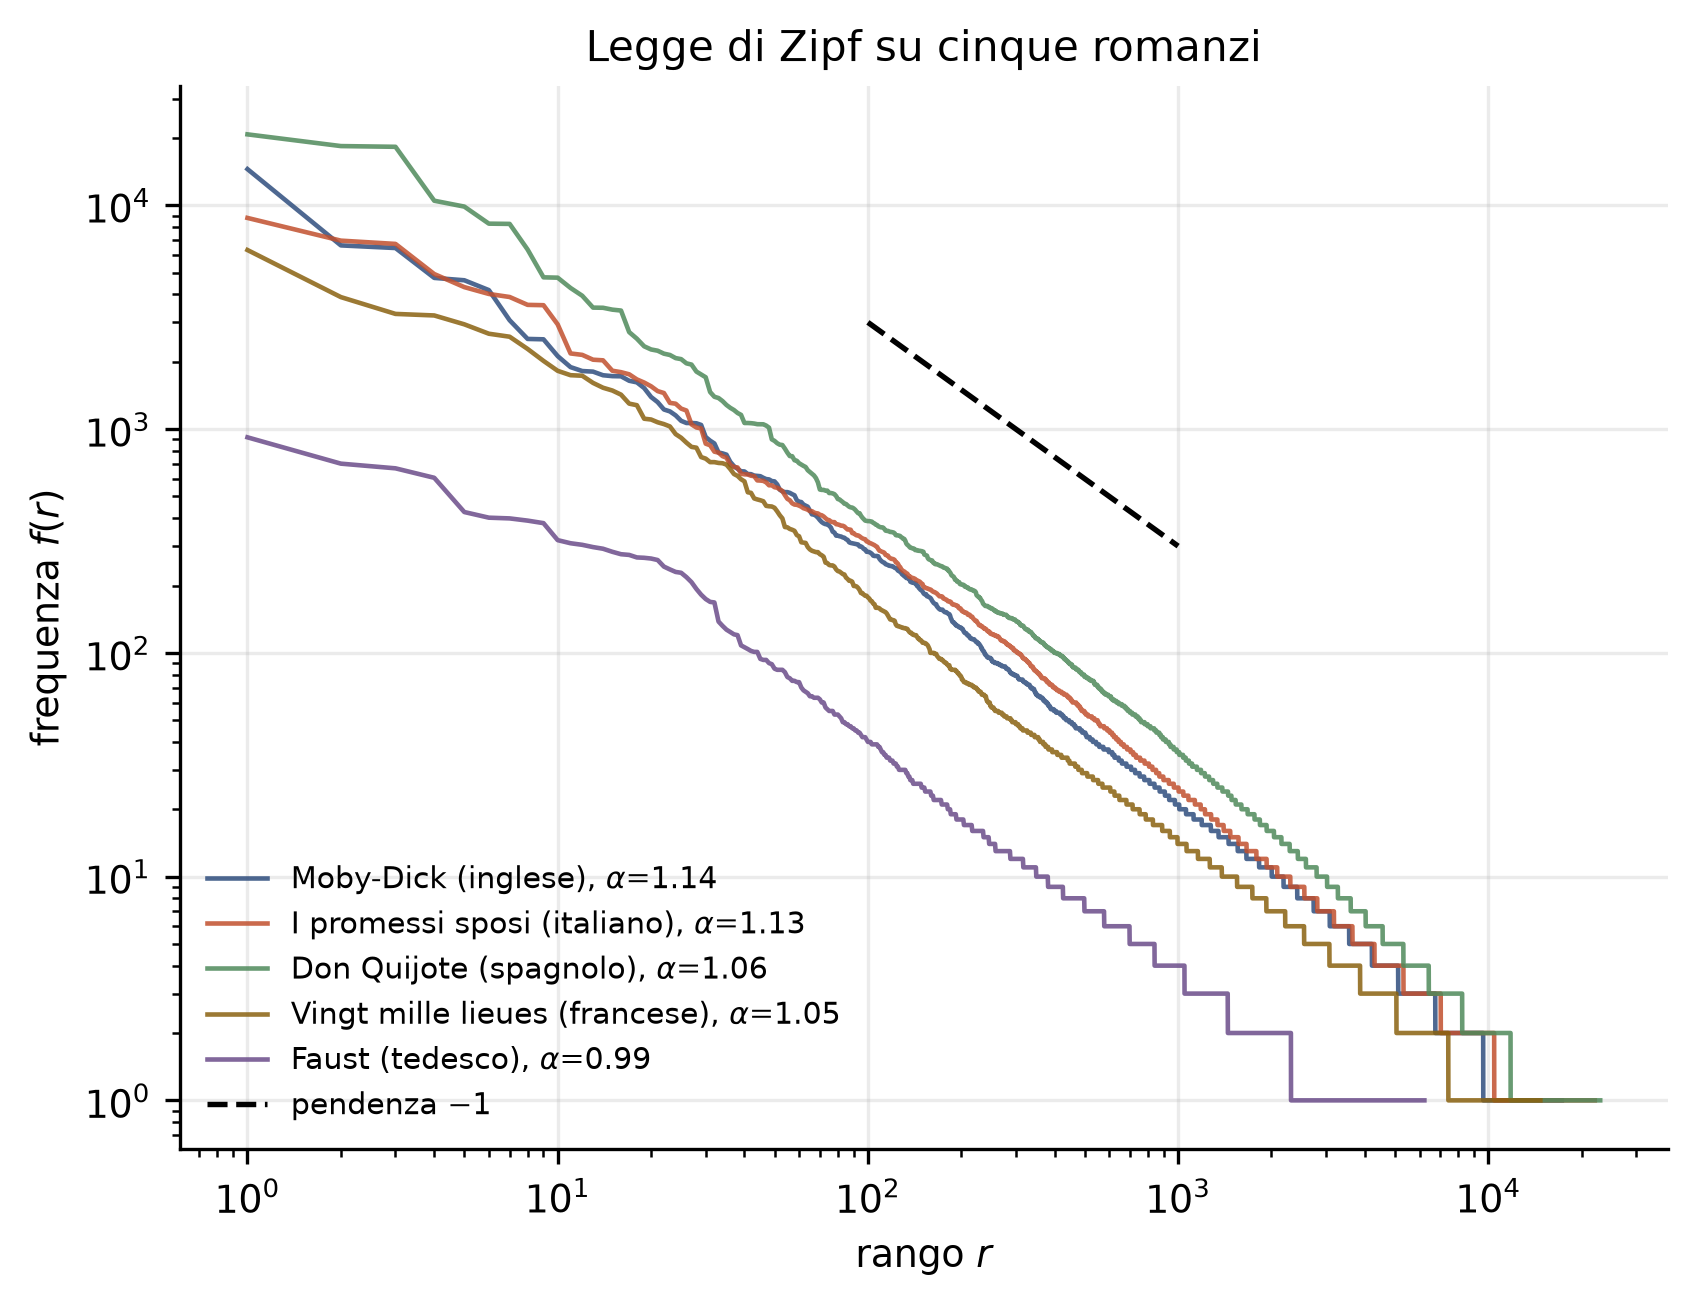
\includegraphics[width=0.82\textwidth]{figure/cap2_zipf_lingue.png}
  \caption{Relazione rango-frequenza per cinque romanzi in altrettante lingue,
  in coordinate bilogaritmiche. Gli esponenti riportati in legenda sono stimati
  per regressione ai minimi quadrati nella finestra di ranghi
  $10^2 \le r \le 10^3$, la stessa impiegata in~\cite{lippi2019}. La retta
  tratteggiata ha pendenza $-1$ ed è riportata come riferimento visivo.}
  \label{fig:zipf}
\end{figure}

Il parametro $\alpha$ risulta positivo e prossimo a 1 nella grande maggioranza
delle lingue esaminate, comprese quelle estinte e quelle costruite
artificialmente. Valori di
$\alpha$ più alti sono sintomo di un vocabolario più povero, poiché un numero
minore di parole esaurisce la maggior parte del testo; valori più bassi
segnalano al contrario una presenza più marcata di parole rare.

I valori misurati sulle cinque opere della Figura~\ref{fig:zipf} sono raccolti
nella Tabella~\ref{tab:zipf-misure}, accanto ai valori medi per lingua riportati
in~\cite{mikhaylovskiy2025zipf} su un corpus di sei opere letterarie in cinque
lingue.

\begin{table}[htbp]
\centering
\small
\begin{tabular}{@{}llrrr@{}}
\toprule
Opera & Lingua & Parole & $|\mathcal{D}|$ & $\alpha$ \\
\midrule
Moby-Dick               & inglese   & \num{219081} & \num{17258} & 1.14 \\
I promessi sposi        & italiano  & \num{239353} & \num{22040} & 1.13 \\
Don Quijote             & spagnolo  & \num{383633} & \num{22943} & 1.06 \\
Vingt mille lieues sous les mers & francese & \num{148923} & \num{14716} & 1.05 \\
Faust                   & tedesco   & \num{30959}  & \num{6221}  & 0.99 \\
\bottomrule
\end{tabular}
\caption{Esponente di Zipf misurato sulle cinque opere della
Figura~\ref{fig:zipf}, con il numero di occorrenze e la dimensione del
dizionario. La stima è condotta sui ranghi $10^2$--$10^3$.}
\label{tab:zipf-misure}
\end{table}

\begin{table}[htbp]
\centering
\small
\begin{tabular}{@{}lcccc@{}}
\toprule
& \multicolumn{2}{c}{$\alpha$ (Zipf)} & \multicolumn{2}{c}{$\gamma_H$ (Heaps)} \\
\cmidrule(lr){2-3}\cmidrule(lr){4-5}
Lingua & parole & token & parole & token \\
\midrule
inglese  & $0.952 \pm 0.072$ & $0.985 \pm 0.054$ & $0.809 \pm 0.027$ & $0.802 \pm 0.024$ \\
tedesco  & $0.959 \pm 0.054$ & $1.024 \pm 0.042$ & $0.846 \pm 0.031$ & $0.793 \pm 0.028$ \\
russo    & $1.043 \pm 0.077$ & $1.009 \pm 0.067$ & $0.916 \pm 0.049$ & $0.805 \pm 0.025$ \\
spagnolo & $0.962 \pm 0.030$ & $1.016 \pm 0.035$ & $0.842 \pm 0.025$ & $0.798 \pm 0.028$ \\
francese & $0.963 \pm 0.033$ & $0.989 \pm 0.042$ & $0.843 \pm 0.020$ & $0.801 \pm 0.018$ \\
\bottomrule
\end{tabular}
\caption{Esponenti medi per lingua riportati in~\cite{mikhaylovskiy2025zipf},
misurati su sei opere letterarie per ciascuna lingua, a livello di parola e di
token. In quel lavoro $\alpha$ è stimato sulla rappresentazione
cumulata della distribuzione anziché sulla relazione rango-frequenza; i due
stimatori coincidono soltanto nel limite $\alpha \to 1$, e i valori non vanno
quindi confrontati direttamente con quelli della
Tabella~\ref{tab:zipf-misure}.}
\label{tab:zipf-letteratura}
\end{table}

Sui testi reali si osservano deviazioni sistematiche dalla~\eqref{eq:zipf}. Su
corpora molto ampi l'esponente resta prossimo a 1 soltanto per le prime migliaia
di parole, mentre la coda continua a seguire una legge di potenza ma con
esponente maggiore~\cite{piantadosi2014}. Le parole più frequenti, inoltre,
mostrano frequenze leggermente inferiori a quelle previste: una deviazione che
Mandelbrot~\cite{mandelbrot1953} corregge introducendo un termine additivo nel
rango,
\begin{equation}
  f(r) \;\propto\; (r + c)^{-\alpha},
  \label{eq:mandelbrot}
\end{equation}
dove la costante $c > 0$ attenua la divergenza della legge di potenza ai ranghi
più bassi, spostando di fatto l'origine dell'asse dei ranghi e rendendo il fit
aderente anche nella regione delle parole più comuni.

\paragraph{Bontà del fit.}
Come si vedrà nei capitoli sperimentali, sui testi generati automaticamente
l'aderenza alla legge di potenza non è garantita. Il solo esponente non è
sufficiente a stabilirla, perché descrive la pendenza media della curva e non la
sua forma: una curva marcatamente incurvata in coordinate bilogaritmiche può
avere la stessa pendenza media di una retta, e restituire quindi un valore di
$\alpha$ del tutto ordinario pur non essendo una legge di potenza. Occorre
perciò una seconda quantità, che misuri quanto i dati si discostino dalla retta
interpolante.

Seguendo~\cite{mikhaylovskiy2025zipf}, la qualità del fit viene stimata con
l'errore percentuale assoluto medio
\begin{equation}
  \mathrm{MAPE} \;=\; \frac{1}{n}\sum_{i=1}^{n}
  \left| \frac{y_i - \hat{y}_i}{y_i} \right|,
  \label{eq:mape}
\end{equation}
dove $n$ è il numero di punti su cui è condotta la regressione, $y_i$ il valore
osservato e $\hat{y}_i$ quello previsto dalla retta interpolante in
corrispondenza dello stesso rango. Il MAPE è nullo per dati perfettamente
allineati e cresce al crescere della distanza relativa dalla retta;
essendo definito su scarti relativi, non dipende dall'unità di misura né
dall'ampiezza delle frequenze, e resta quindi confrontabile fra testi di
lunghezza diversa.

Sul corpus di testi letterari usato in~\cite{mikhaylovskiy2025zipf} il MAPE vale
in media $0.156$ con deviazione standard $0.077$. Nei capitoli sperimentali il
suo minimo in funzione della temperatura di generazione individuerà il regime in
cui il testo prodotto è più vicino a una legge di potenza.

% ---------------------------------------------------------------------
\subsection{Legge di Heaps}
\label{sec:heaps}

Studiando l'andamento di $|\mathcal{D}(t)|$ nei testi letterari emerge una
seconda regolarità, nota come legge di Heaps o, dal nome di chi la formulò per
primo~\cite{herdan1964}, di Herdan--Heaps:
\begin{equation}
  |\mathcal{D}(t)| \;\propto\; t^{\gamma_H}, \qquad \gamma_H \in [0,1] .
  \label{eq:heaps}
\end{equation}
Qui $t$ è la posizione nel testo, misurata in numero di parole,
$|\mathcal{D}(t)|$ la dimensione del dizionario parziale e $\gamma_H$
l'esponente di Heaps. I due estremi dell'intervallo corrispondono a due
comportamenti limite: $\gamma_H = 0$ descrive un dizionario che cessa di
crescere, cioè un testo che non introduce più parole nuove, mentre
$\gamma_H = 1$ descrive un dizionario che cresce proporzionalmente alla
lunghezza, cioè un testo in cui ogni parola è nuova. Poiché il dizionario non
può crescere più rapidamente del testo che lo contiene, si ha necessariamente
$|\mathcal{D}(t)| \le t$, e l'esponente non può eccedere l'unità.

La legge di Heaps quantifica dunque la capacità di un testo di rinnovare il
proprio vocabolario, ed è per questo particolarmente istruttiva se si torna alla
Tabella~\ref{tab:tre-regimi} del Capitolo~\ref{cap:introduzione}. Il primo
esempio, monotono e ripetitivo, cessa rapidamente di accrescere il dizionario;
l'ultimo, in cui i caratteri sono estratti a caso, produce quasi soltanto parole
nuove e fa crescere il dizionario senza saturare. La Figura~\ref{fig:heaps}
mostra le curve dei due casi limite accanto a quelle di tre testi letterari.

\begin{figure}[htbp]
  \centering
  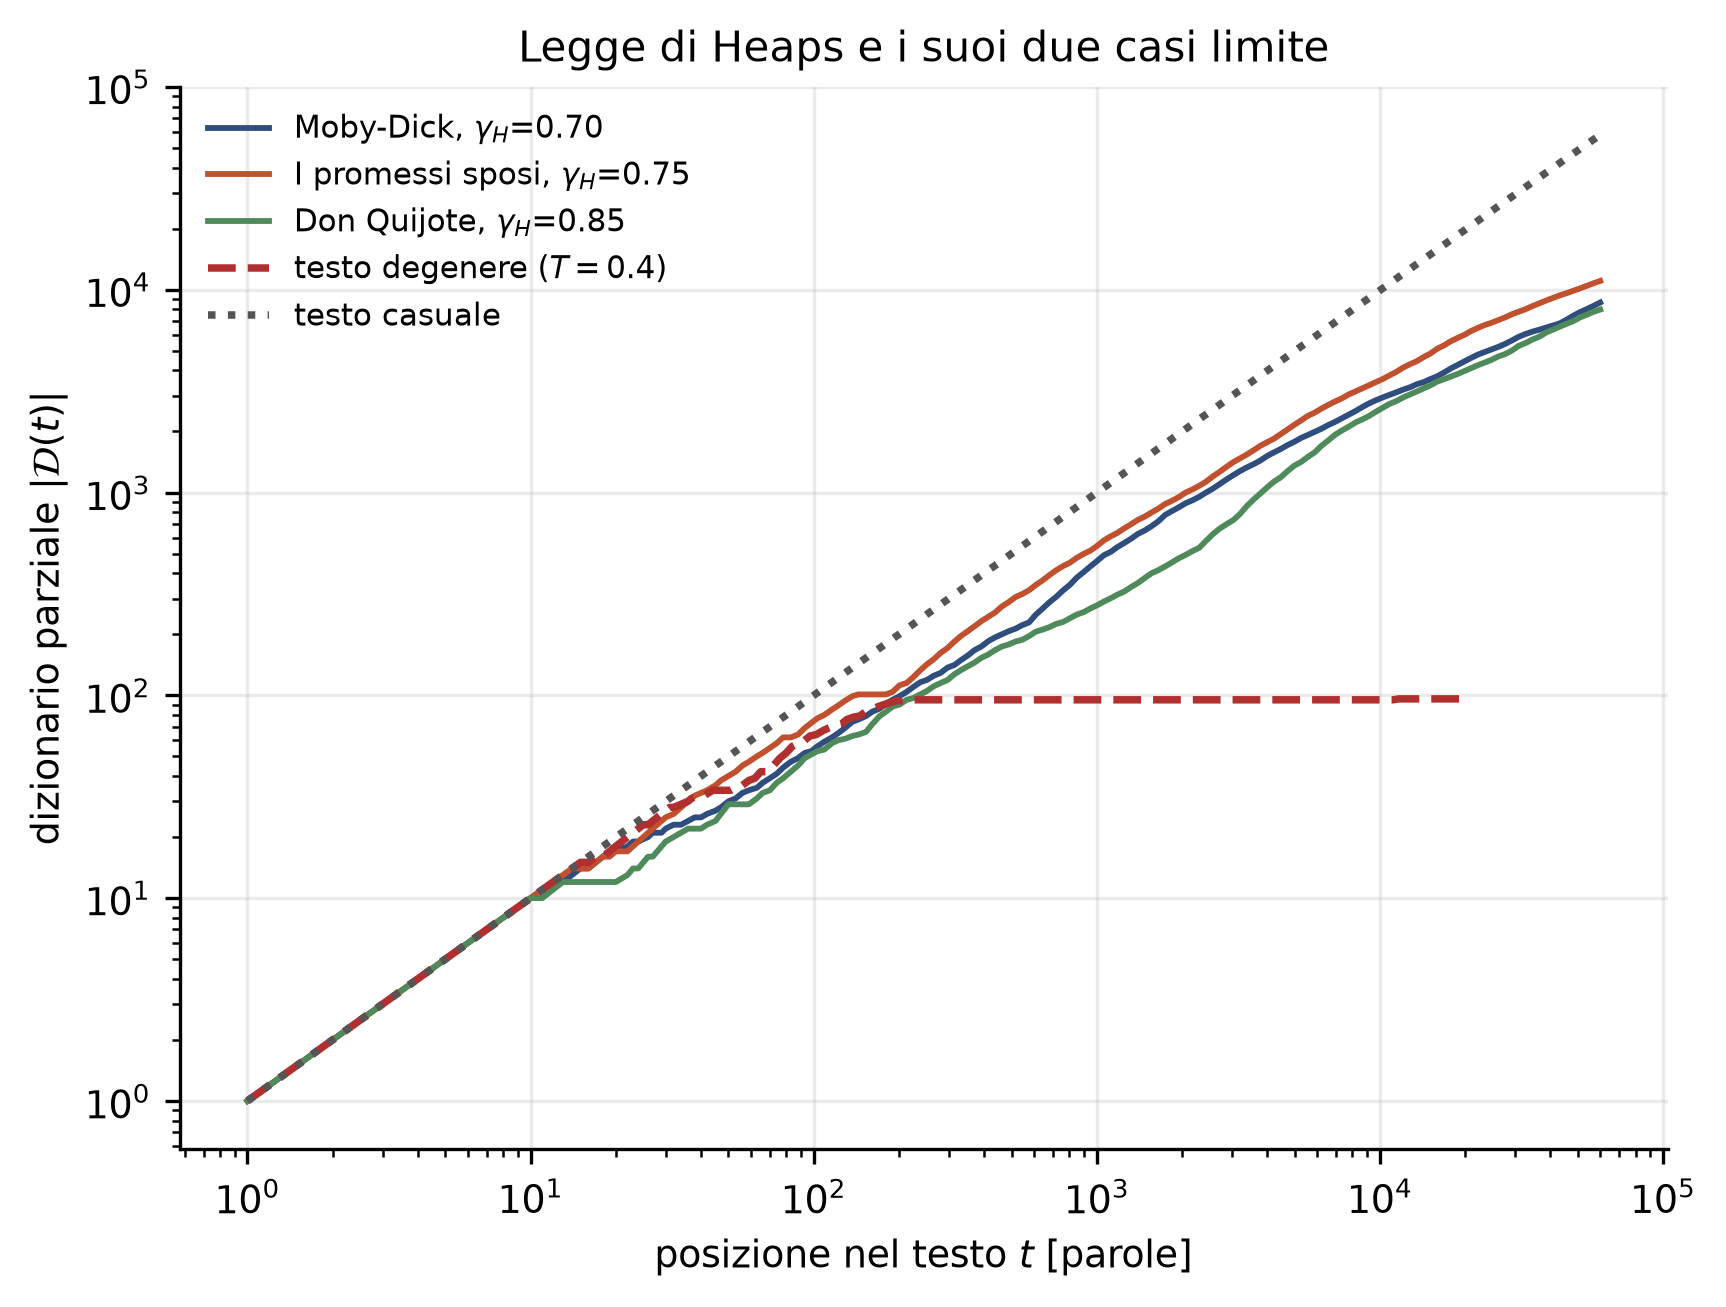
\includegraphics[width=0.82\textwidth]{figure/cap2_heaps_confronto.png}
  \caption{Crescita del dizionario parziale in coordinate bilogaritmiche. Le tre
  curve continue sono testi letterari, con esponente stimato nella regione
  $t > 1000$. La curva tratteggiata è il campione generato a $T = 0.4$ già
  riportato nella Tabella~\ref{tab:tre-regimi}: dopo circa un centinaio di
  parole entra in un ciclo di ripetizione e il dizionario si arresta. La curva
  punteggiata è una sequenza di caratteri casuali, in cui ogni parola è nuova e
  la crescita è esattamente lineare.}
  \label{fig:heaps}
\end{figure}

L'esponente stimato dipende inoltre dall'intervallo su cui viene condotta la
regressione, e quindi dalla lunghezza del testo analizzato. La
Figura~\ref{fig:heaps-finito} mostra l'effetto su tre opere: ripetendo la stima
su prefissi via via più lunghi della stessa opera, $\gamma_H$ decresce in modo
sistematico, di oltre un decimo fra $10^4$ e $10^5$ parole. Il fenomeno è la
prima manifestazione degli effetti di dimensione finita discussi in modo
generale nel §\ref{sec:lunghezza}, ed è già segnalato
in~\cite{mikhaylovskiy2025zipf}, dove si osserva che per $\alpha$ prossimo a 1
la crescita del dizionario è descritta meglio dalla forma $t/\ln t$ che da una
pura legge di potenza. Ai valori di $N$ più bassi la regressione si appoggia a
un intervallo troppo corto e può restituire stime superiori a 1, incompatibili
con il limite teorico: è un artefatto della finestra di fit, non una proprietà
del testo.

\begin{figure}[htbp]
  \centering
  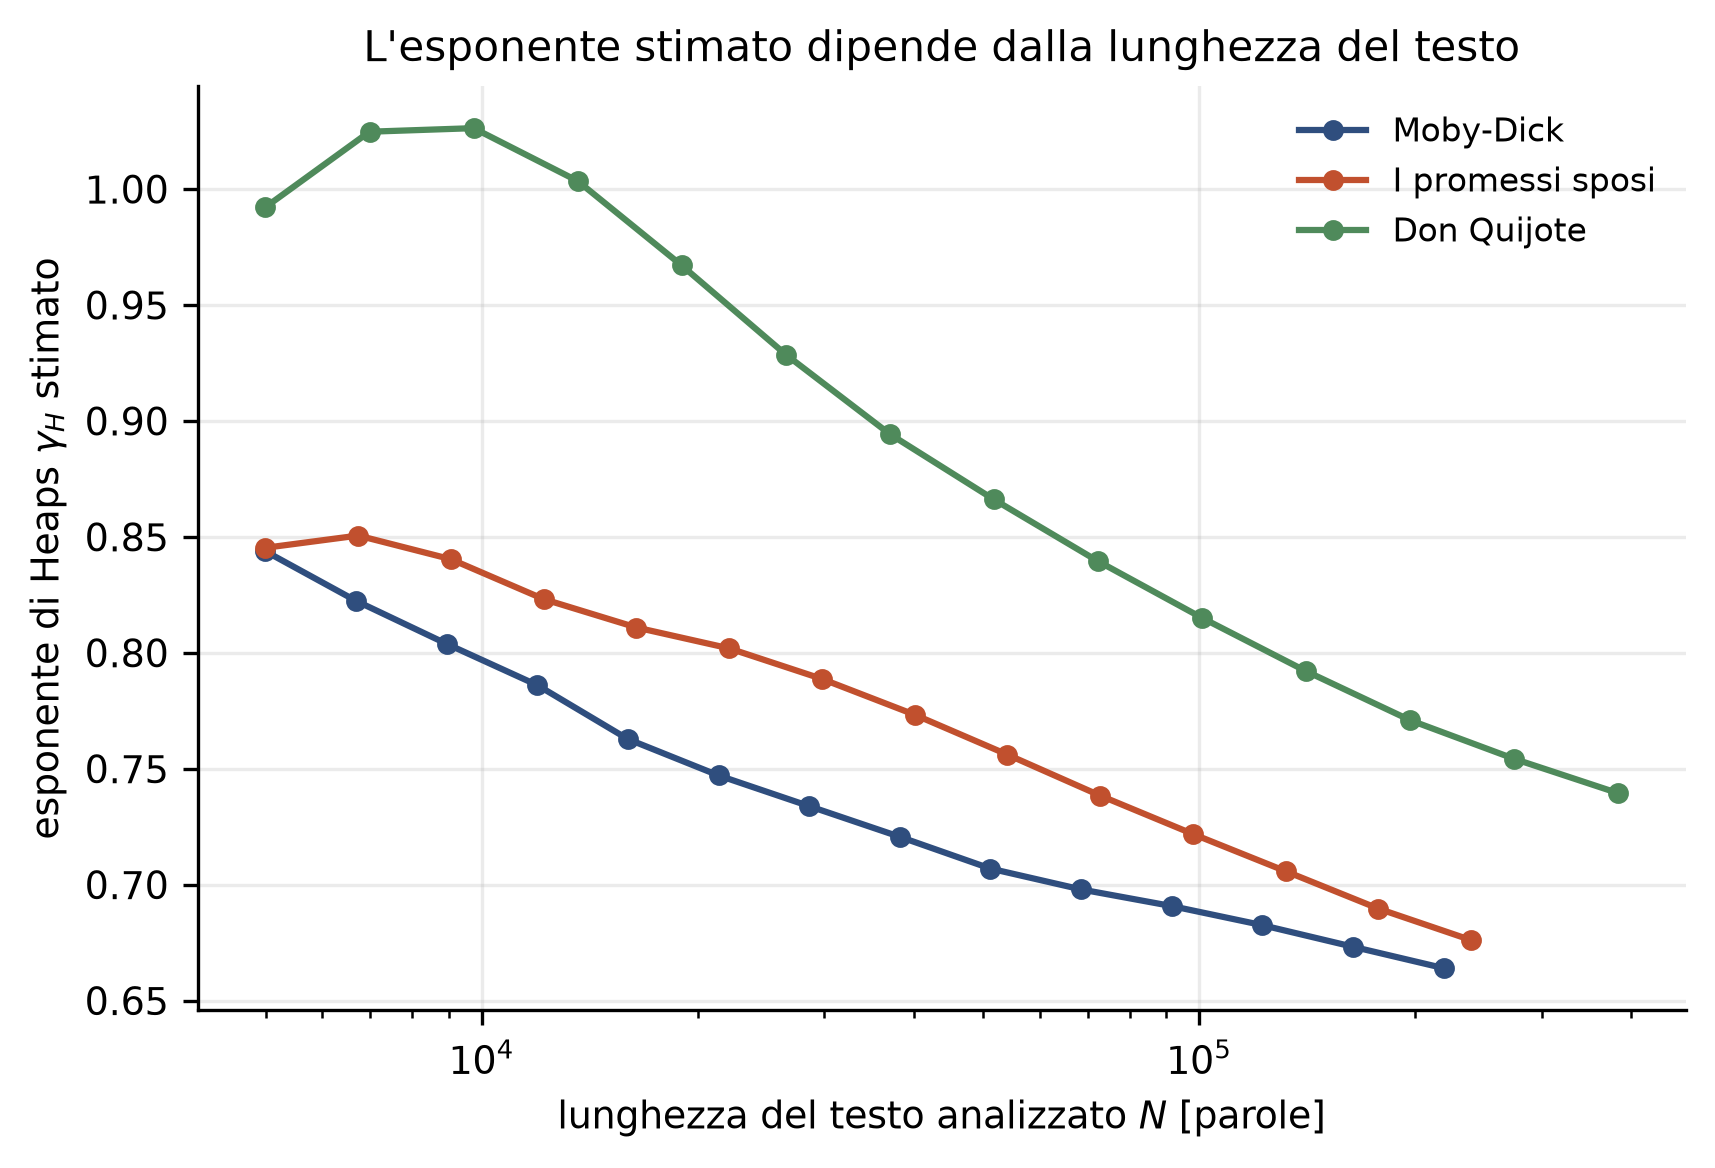
\includegraphics[width=0.78\textwidth]{figure/cap2_heaps_dimensione_finita.png}
  \caption{Esponente di Heaps stimato su prefissi di lunghezza crescente, per tre
  opere in tre lingue diverse, con regressione condotta nella regione $t > 1000$.
  La deriva è sistematica e comune a tutte e tre, ed è quindi una proprietà dello
  stimatore e non di una particolare opera: confrontare esponenti misurati su
  testi di lunghezza diversa non è lecito. Il §\ref{sec:scelte} riprende
  l'effetto su una sola opera, misurandone però l'entità su tutti gli stimatori
  impiegati in questa tesi.}
  \label{fig:heaps-finito}
\end{figure}

\paragraph{Il descrittore $R$.}
Sui testi generati automaticamente la difficoltà è più radicale. A bassa
temperatura di generazione il modello entra in un ciclo di ripetizione e cessa
di produrre parole nuove: la curva $|\mathcal{D}(t)|$ diventa piatta e
la~\eqref{eq:heaps} perde significato. Ad alta temperatura si verifica il caso
opposto, con quasi ogni parola nuova e curva prossima alla linearità. In
entrambe le situazioni la stima di $\gamma_H$ restituisce un numero privo di
contenuto, come mostrano le due curve estreme della Figura~\ref{fig:heaps}.

Per questa ragione in~\cite{mikhaylovskiy2025zipf} viene introdotto un
descrittore che resta definito in ogni regime. Detti $\mathcal{D}_1$ il
dizionario della prima metà del testo e $\mathcal{D}_2$ quello della seconda, si
pone
\begin{equation}
  R \;=\; \frac{|\mathcal{D}_2 \setminus \mathcal{D}_1|}{|\mathcal{D}_1|},
  \label{eq:R}
\end{equation}
cioè il rapporto fra il numero di parole che compaiono per la prima volta nella
seconda metà del testo e il numero di quelle che compaiono per la prima volta
nella prima. Un testo degenerato ha $R$ prossimo a zero, poiché la seconda metà
non introduce nulla di nuovo; un testo in cui ogni parola è nuova ha $R$
prossimo a uno. Sul corpus di opere letterarie intere usato
in~\cite{mikhaylovskiy2025zipf} il valore medio è $R = 0.17$ con deviazione
standard $0.05$.


% ---------------------------------------------------------------------
\section{Correlazioni a lungo raggio}
\label{sec:lrc}

Sia la legge di Zipf sia quella di Heaps ignorano l'ordine dei simboli. Per la
prima l'affermazione è immediata: la~\eqref{eq:zipf} dipende soltanto dai
conteggi delle parole, e un rimescolamento del testo li lascia invariati. Per la
seconda l'invarianza è meno diretta: rimescolando il testo la curva
$|\mathcal{D}(t)|$ cambia realizzazione, perché cambia l'ordine in cui le
parole compaiono per la prima volta, ma il suo andamento medio resta lo stesso, e con esso l'esponente
$\gamma_H$. Entrambe sono quindi proprietà del vocabolario, non della sequenza.

Per misurare le proprietà che dipendono dall'ordine occorre estrarre dal testo
un segnale, cioè una successione finita di valori reali, e studiarne le
correlazioni a scale diverse. La costruzione del segnale non è unica, e ogni
scelta mette in luce aspetti differenti: si può codificare la posizione delle
singole lettere o di classi di lettere, quella delle parole o di classi
grammaticali, oppure la lunghezza delle frasi. In tutti i casi si osserva che il
linguaggio esibisce correlazioni a lungo raggio, con una struttura che si
estende su molti ordini di grandezza~\cite{altmann2012,montemurro2002}.

% ---------------------------------------------------------------------
\subsection{Funzione di autocorrelazione}
\label{sec:acf}

Data una successione $x_1,\dots,x_N$, la funzione di autocorrelazione a distanza
$s$ è
\begin{equation}
  c(s) \;=\; \langle x_n x_{n+s}\rangle
  - \langle x_n\rangle\langle x_{n+s}\rangle ,
  \label{eq:acf}
\end{equation}
dove $\langle\cdot\rangle$ indica la media su tutte le posizioni $n$ compatibili
con la distanza $s$. La forma funzionale di $c(s)$ distingue i regimi di
correlazione.

Se i valori non sono correlati, $c(s)$ è identicamente nulla per $s \neq 0$. Se
$c(s)$ decade esponenzialmente,
$c(s) \sim e^{-s/s_0}$, il segnale si dice correlato a corto raggio: la costante
$s_0$ ha le dimensioni di una distanza e ne fissa la scala caratteristica, nel
senso che oltre poche volte $s_0$ la correlazione è numericamente
indistinguibile da zero. Esiste dunque una distanza tipica oltre la quale due
porzioni di segnale sono indipendenti, e il sistema non possiede struttura al di
là di essa.

Si dice invece che il segnale è correlato a lungo raggio quando il decadimento
segue la legge di potenza
\begin{equation}
  c(s) \;\sim\; s^{-\theta},
  \label{eq:acf-power}
\end{equation}
con $0<\theta<1$. In questo caso non esiste alcuna scala privilegiata: la
funzione~\eqref{eq:acf-power} è invariante di scala, cioè riscalare $s$ di un
fattore costante riscala $c$ di un fattore costante senza modificarne la forma,
e un certo grado di correlazione persiste a tutte le distanze.\footnote{L'esponente
qui indicato con $\theta$ è denotato con $\beta$ in~\cite{altmann2012} e con
$\gamma$ in altra parte della letteratura. Il simbolo è stato cambiato per
evitare la collisione con l'esponente di Heaps e con quello introdotto
nella~\eqref{eq:sigma}.}

La stima diretta di $\theta$ dalla~\eqref{eq:acf-power} è però problematica. Il
segnale è affetto da rumore e, soprattutto, da tendenze di origine esterna che
non sono oggetto di interesse: se la media $\langle x_n\rangle$ differisce fra
la prima e la seconda metà del segnale, come accade proprio quando le
correlazioni sono forti, la~\eqref{eq:acf} risulta distorta. L'esponente va
quindi stimato per via indiretta, e le due sottosezioni seguenti presentano i
due metodi impiegati in questa tesi.

% ---------------------------------------------------------------------
\subsection{Indicatore integrato}
\label{sec:integrato}

Il primo metodo è quello adottato da Altmann, Cristadoro e Degli
Esposti~\cite{altmann2012}, e si applica a segnali binari. Sia dato un testo
come successione simbolica $s = (s_1,\dots,s_N)$. Si definisce una condizione
locale $\mathcal{A}$ che genera la successione binaria
\begin{equation}
  x_k \;=\;
  \begin{cases}
    1 & \text{se $\mathcal{A}$ è soddisfatta in posizione $k$},\\
    0 & \text{altrimenti}.
  \end{cases}
  \label{eq:osservabile}
\end{equation}
L'osservabile può essere la presenza di una data lettera, di una data parola,
oppure l'appartenenza a una classe: per esempio se la lettera in posizione $k$ è
una vocale. L'unità di misura della distanza è il numero di simboli del livello
considerato, ed è questa scelta a rendere confrontabili fra loro una successione
di lettere e una di parole.

Posto
\begin{equation}
  X(t) \;=\; \sum_{j \le t} x_j ,
  \label{eq:conteggio}
\end{equation}
cioè il numero di occorrenze osservate nelle prime $t$ posizioni, si studia la
crescita della varianza del conteggio
\begin{equation}
  \sigma_X^2(t) \;=\; \langle X(t)^2\rangle - \langle X(t)\rangle^2
  \;\simeq\; t^{\gamma}, \qquad \gamma = 2 - \theta .
  \label{eq:sigma}
\end{equation}
La quantità $\sigma_X^2$ è, per costruzione, una somma delle correlazioni a
tutte le distanze inferiori a $t$, e come tale è numericamente assai più stabile
della~\eqref{eq:acf} stimata punto per punto.

Il discrimine fra correlazioni a corto e a lungo raggio non è l'ampiezza di
$c(s)$, ma la sua sommabilità. La~\eqref{eq:conteggio} è formalmente il
cammino percorso da un camminatore che a ogni passo avanza di $x_j$: se i passi
sono indipendenti, o abbastanza rapidamente decorrelati perché $\sum_s c(s)$
converga, vale il teorema del limite centrale e la varianza del cammino cresce
proporzionalmente al numero di passi. Si ha allora diffusione normale,
$\gamma = 1$, esattamente come per il moto browniano. Se invece la somma
diverge, cioè se $\theta \le 1$, i passi restano correlati a ogni scala, il
camminatore tende a proseguire nella direzione già intrapresa e si allontana
dall'origine più rapidamente: la diffusione è anomala e $1 < \gamma < 2$. Il
valore $\gamma = 1$ costituisce dunque il riferimento nullo di tutte le misure
di questo tipo.

La stima di $\gamma$ risente di effetti di tempo finito che la fanno
sottostimare~\cite{altmann2012}: tutti i valori riportati nei capitoli
sperimentali vanno letti come limiti inferiori.

% ---------------------------------------------------------------------
\subsection{Detrended fluctuation analysis}
\label{sec:dfa}

Il secondo metodo è la \emph{detrended fluctuation analysis}, introdotta da
Peng et al.~\cite{peng1994} e applicata ai testi generati automaticamente
in~\cite{lippi2019}. Rispetto all'indicatore integrato presenta il vantaggio
di rimuovere le tendenze locali, e risulta quindi applicabile anche a segnali
non stazionari, cioè segnali le cui proprietà statistiche, tipicamente la
media $\langle x_n \rangle$ o la varianza, non sono costanti lungo la
successione ma derivano lentamente da un estremo all'altro.

La distinzione fra tendenza e correlazione è essenziale, e non riguarda solo
l'origine delle due. Una tendenza è una deriva sistematica e regolare del valore
medio, sovrapposta al segnale da una causa esterna al sistema; una correlazione
è invece una proprietà statistica interna, che lega fra loro le fluttuazioni
attorno a quel valore medio. Il problema pratico è che entrambe producono lo
stesso effetto sulla~\eqref{eq:acf}, gonfiandola a grandi distanze, ed è quindi
necessario eliminare le prime per misurare le seconde. Si potrebbe pensare
sufficiente sottrarre una media mobile di ampiezza fissata, ma in questo modo si
introdurrebbe artificialmente nei dati proprio quella ampiezza come scala
caratteristica, distruggendo le altre.

Il segnale viene costruito codificando ogni carattere del testo con il proprio
rango di frequenza: al carattere più frequente si associa 1, al secondo 2, e
così via. Seguendo~\cite{lippi2019} la codifica avviene a livello di carattere e
conserva punteggiatura, cifre, maiuscole e lettere accentate. Ottenuta la
successione $x_i$ con $i = 1,\dots,N$, la procedura si articola in quattro
passi, qui presentati nella formulazione di~\cite{kantelhardt2001}.

\begin{enumerate}
  \item Si determina il profilo
    \begin{equation}
      Y(i) \;=\; \sum_{k=1}^{i}\bigl(x_k - \langle x\rangle\bigr),
      \label{eq:dfa-profilo}
    \end{equation}
    cioè lo scarto cumulato dalla media. La sottrazione della media non è
    strettamente necessaria, poiché verrebbe comunque eliminata dal detrending.
  \item Si divide il profilo in $N_s = \lfloor N/s \rfloor$ segmenti disgiunti
    di lunghezza $s$.
  \item In ciascun segmento si interpola ai minimi quadrati la tendenza locale,
    ottenendo il polinomio $Y_s(i)$ che approssima il profilo entro quel
    segmento. L'ordine del polinomio determina l'ordine delle tendenze rimosse:
    una DFA di ordine $n$ elimina le tendenze polinomiali fino al grado $n$. In
    questa tesi si impiega l'ordine 1, che rimuove le tendenze lineari locali;
    la robustezza dei risultati rispetto a questa scelta è verificata nel
    §\ref{sec:robustezza}.
  \item Si calcola lo scarto quadratico medio del profilo dalla propria
    tendenza locale, mediando su tutti i segmenti, e si ottiene la funzione di
    fluttuazione
    \begin{equation}
      F(s) \;=\; \left(\frac{1}{N}\sum_{i=1}^{N}
      \bigl(Y(i) - Y_s(i)\bigr)^2\right)^{1/2}.
      \label{eq:dfa-F}
    \end{equation}
\end{enumerate}

La fluttuazione cresce con la lunghezza dei segmenti $s$ e, per un segnale
correlato a lungo raggio, segue la legge di potenza
\begin{equation}
  F(s) \;\sim\; s^{\alpha_{\mathrm{DFA}}} .
  \label{eq:dfa-alpha}
\end{equation}
Per un segnale scorrelato, o correlato a corto raggio, si ha
$\alpha_{\mathrm{DFA}} = 1/2$. Valori superiori indicano correlazioni
persistenti: una fluttuazione positiva tende a essere seguita da un'altra
fluttuazione positiva, e il segnale conserva memoria della propria direzione.
Valori inferiori indicano correlazioni antipersistenti, in cui una fluttuazione
positiva tende a essere seguita da una negativa e il segnale tende a tornare
sui propri passi. Un cammino aleatorio dà $\alpha_{\mathrm{DFA}} = 3/2$: i suoi
incrementi sono scorrelati, ma la successione che ne risulta accumula ogni
deviazione senza riassorbirla, e le fluttuazioni crescono di conseguenza molto
più in fretta. Sul testo letterario di riferimento~\cite{lippi2019} riporta
$\alpha_{\mathrm{DFA}} \simeq 0.65$, contro $0.50$ misurato sulla sua versione
rimescolata: nettamente sopra il riferimento scorrelato e nettamente sotto
quello del cammino aleatorio.

% ---------------------------------------------------------------------
\subsection{Relazione fra i due metodi}
\label{sec:ponte}

I due metodi introdotti misurano la stessa proprietà, e i rispettivi esponenti
sono legati da una relazione semplice. Applicata alla medesima successione,
la~\eqref{eq:dfa-F} coincide, a meno del detrending, con la deviazione standard
del profilo alla scala $s$, cioè $F(s) \simeq \sigma_X(s)$. Elevando al quadrato
e usando la~\eqref{eq:sigma} si ottiene $F(s)^2 \simeq s^{\gamma}$, da cui
\begin{equation}
  \alpha_{\mathrm{DFA}} \;=\; \frac{\gamma}{2} \;=\; 1 - \frac{\theta}{2} .
  \label{eq:ponte}
\end{equation}
La stessa relazione, ricavata per altra via, è riportata
in~\cite{kantelhardt2001}. Nella~\eqref{eq:ponte} $\gamma$ è l'esponente di
crescita della varianza del conteggio definito nella~\eqref{eq:sigma}, mentre
$\theta$ è l'esponente di decadimento dell'autocorrelazione definito
nella~\eqref{eq:acf-power}; i tre esponenti sono dunque tre modi equivalenti di
esprimere la stessa proprietà del segnale.

La~\eqref{eq:ponte} costituisce il ponte fra le due parti sperimentali della
tesi: la diffusione normale $\gamma = 1$, riferimento nullo dell'analisi di
burstiness, corrisponde esattamente al valore $\alpha_{\mathrm{DFA}} = 1/2$,
riferimento nullo dell'analisi sui testi generati. Le due misure non coincidono
esattamente sui dati, poiché la detrended fluctuation analysis rimuove le
tendenze locali mentre l'indicatore integrato no; la differenza fra i due
risultati è informativa proprio quando il segnale non è stazionario.

Un caso limite si presenta con frequenza nei testi generati a bassa
temperatura. Se il testo degenera in un ciclo di ripetizione,
la successione $x_i$ diventa quasi periodica e il profilo~\eqref{eq:dfa-profilo}
oscilla invece di allontanarsi dall'origine: la fluttuazione satura oltre la
lunghezza del periodo e $\alpha_{\mathrm{DFA}}$ scende verso zero. Un esponente
molto basso non segnala quindi assenza di struttura, ma struttura periodica, e
va interpretato congiuntamente a un indicatore diretto di ripetizione.


% ---------------------------------------------------------------------
\section{Burstiness e statistica degli intervalli}
\label{sec:burst}

Le sezioni precedenti permettono di stabilire se un testo possieda correlazioni
a lungo raggio. Questa sezione introduce gli strumenti necessari a stabilire
l'origine di tali correlazioni, che è la domanda posta in~\cite{altmann2012} e
ripresa nella seconda parte sperimentale.

Il punto di partenza è un'osservazione elementare sulla distribuzione delle
parole lungo il testo. Non tutte le parole si distribuiscono allo stesso modo:
alcune ricorrono in modo pressoché uniforme dall'inizio alla fine, altre si
addensano nelle sezioni che trattano l'argomento cui appartengono e sono quasi
assenti altrove. La Figura~\ref{fig:barcode} rende visibile la differenza. Ogni
barra verticale segna una posizione in cui la parola compare; nel primo pannello
la parola è un articolo, nel secondo il nome di un personaggio.

\begin{figure}[htbp]
  \centering
  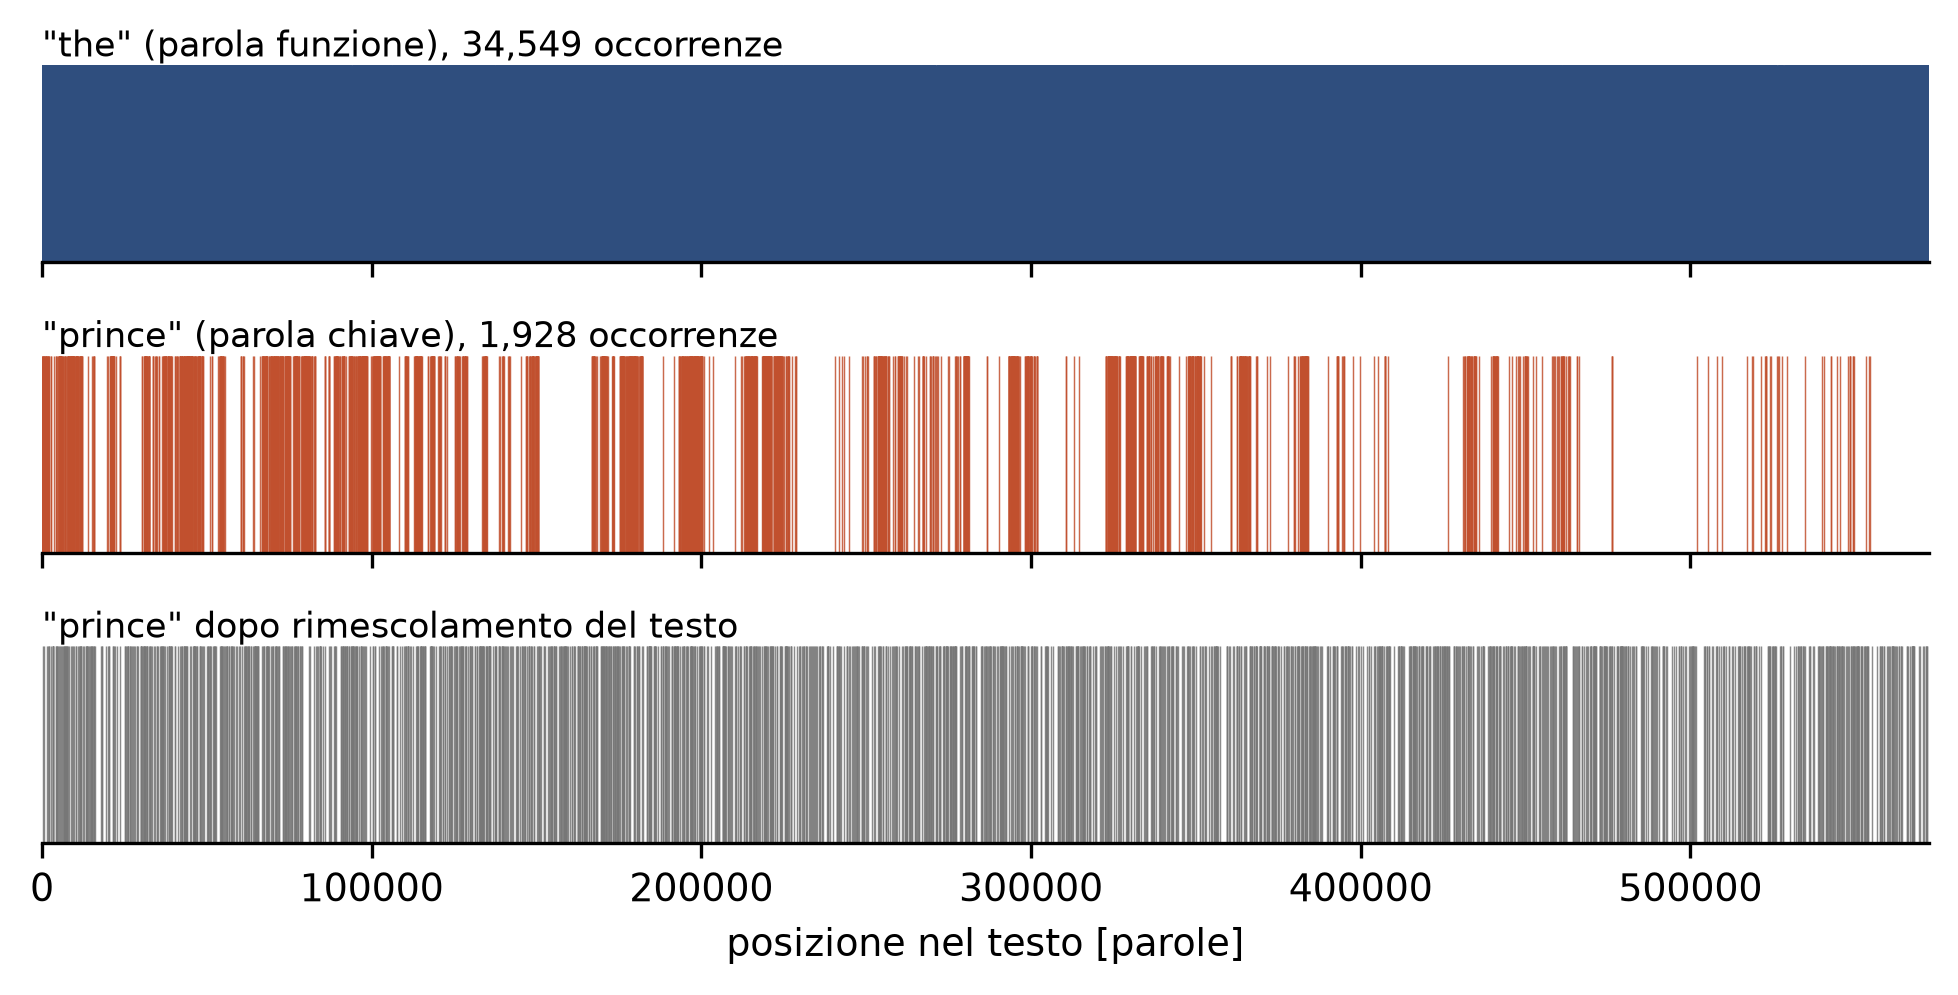
\includegraphics[width=\textwidth]{figure/cap2_burstiness_barcode.png}
  \caption{Posizioni di occorrenza di due parole in \emph{Guerra e pace}. La
  parola funzione \emph{the} riempie il testo in modo uniforme e il pannello
  appare come una banda piena. La parola chiave \emph{prince} si addensa invece
  in gruppi separati da lunghi vuoti, che corrispondono alle porzioni di romanzo
  in cui il personaggio non compare. Il terzo pannello riporta le occorrenze di
  \emph{prince} dopo aver rimescolato le parole del testo: i conteggi sono
  identici, ma i gruppi scompaiono. La struttura visibile nel secondo pannello
  è dunque una proprietà dell'ordine, non delle frequenze.}
  \label{fig:barcode}
\end{figure}

Il fenomeno illustrato dal secondo pannello prende il nome di
\emph{burstiness}: le occorrenze non sono sparse indipendentemente, ma
raggruppate in raffiche separate da intervalli lunghi. Il terzo pannello mostra
perché si tratti di una proprietà dell'ordine e non del vocabolario: il
rimescolamento conserva esattamente il numero di occorrenze, e con esso la legge
di Zipf, ma distrugge la struttura.

Per quantificare il fenomeno si torna alla successione binaria definita
nella~\eqref{eq:osservabile} e si considerano gli intervalli
$\tau_1, \tau_2, \dots$ fra occorrenze consecutive, cioè le distanze in numero
di simboli fra un $1$ e il successivo. La loro distribuzione di probabilità
viene indicata con $p(\tau)$ ed è l'oggetto centrale di questa sezione: tutta
l'informazione sull'ordine che il conteggio delle occorrenze non cattura è
contenuta in $p(\tau)$ e nelle correlazioni fra intervalli successivi.

Il termine di paragone naturale è il processo di Poisson, cioè il processo in
cui ogni posizione ha la stessa probabilità di ospitare un'occorrenza,
indipendentemente da tutte le altre. È il modello del «nessuna struttura»: se le
occorrenze di \emph{prince} fossero poissoniane, il secondo pannello della
Figura~\ref{fig:barcode} sarebbe indistinguibile dal terzo. Per un processo di
Poisson gli intervalli sono distribuiti esponenzialmente e indipendenti fra
loro, e si dimostra che la loro deviazione standard eguaglia la media,
$\sigma_\tau = \langle\tau\rangle$.

Si misura quindi la burstiness con il coefficiente di variazione
\begin{equation}
  \mathrm{cv} \;=\; \frac{\sigma_\tau}{\langle\tau\rangle},
  \label{eq:cv}
\end{equation}
pari a 1 nel caso poissoniano, maggiore di 1 quando le occorrenze si addensano
in raffiche separate da vuoti lunghi e minore di 1 quando sono distribuite in
modo più regolare di quanto il caso comporti. Una misura equivalente, ma
limitata all'intervallo $[-1,1]$ e quindi più comoda per il confronto fra
sequenze diverse, è l'indice proposto da Goh e Barabási~\cite{goh2008},
\begin{equation}
  B \;=\; \frac{\sigma_\tau - \langle\tau\rangle}
                {\sigma_\tau + \langle\tau\rangle} .
  \label{eq:goh}
\end{equation}

% ---------------------------------------------------------------------
\subsection{Le due origini delle correlazioni}
\label{sec:origini}

Il contributo centrale di~\cite{altmann2012} consiste nell'osservare che una
varianza del conteggio che cresce più che linearmente può avere due origini
distinte. Il legame è fornito dallo spettro di potenza a frequenza nulla.

Lo spettro di potenza $S(\omega)$ di una successione descrive come la sua
varianza si distribuisce fra le diverse frequenze $\omega$, ed è la trasformata
di Fourier della funzione di autocorrelazione. Il valore a frequenza nulla,
$S(0)$, raccoglie il contributo delle fluttuazioni più lente, quelle su scale
comparabili con la lunghezza dell'intera successione: è quindi la quantità che
diverge esattamente quando esistono correlazioni a lungo raggio, e che resta
finita quando le correlazioni sono sommabili. Per una successione di occorrenze
descritta dagli intervalli $\tau_i$ vale
\begin{equation}
  S(0) \;=\; \frac{\sigma_\tau^2}{\langle\tau\rangle^3}
  \left(1 + 2\sum_{k\ge1} c_\tau(k)\right),
  \label{eq:eq4}
\end{equation}
dove $c_\tau(k)$ è l'autocorrelazione della successione degli intervalli, cioè
la correlazione fra $\tau_i$ e $\tau_{i+k}$.

La~\eqref{eq:eq4} è il perno dell'intera analisi, perché mostra che $S(0)$ può
divergere in due modi indipendenti. Il primo è la divergenza di $\sigma_\tau$,
cioè una coda pesante di $p(\tau)$: il testo contiene vuoti così lunghi che la
varianza degli intervalli non converge. Il secondo è la non sommabilità di
$c_\tau(k)$, cioè il fatto che gli intervalli siano essi stessi correlati fra
loro. Nella formula resta implicito che cosa questo comporti: $c_\tau(k) > 0$
significa che a un intervallo più lungo della media tende a seguirne un altro
più lungo della media, e quindi che i vuoti si
raggruppano fra loro invece di alternarsi ai riempimenti. Anche con una
$p(\tau)$ a varianza finita, un simile raggruppamento produce fluttuazioni
lente del conteggio e fa divergere la somma.

I due meccanismi sono distinti, perché l'uno riguarda quanto sono lunghi i
vuoti e l'altro come sono disposti, e la~\eqref{eq:eq4} da sola non li separa.

Nei testi reali, di lunghezza finita e con la coda tagliata
(§\ref{sec:coda}), nessuna delle due quantità diverge davvero: ciò che si
misura sono i loro analoghi a finestra finita, e i due null model del
§\ref{sec:null} servono appunto a separarli senza dover decidere quale delle
due divergenze sarebbe realizzata nel limite.

% ---------------------------------------------------------------------
\subsection{I null model A1 e A2}
\label{sec:null}

La separazione si ottiene con due rimescolamenti controllati, costruiti in modo
da distruggere selettivamente uno solo dei due meccanismi.

Il primo, indicato con A1, permuta gli zeri e gli uni della successione binaria.
Conserva soltanto il numero di occorrenze e distrugge tanto la coda di $p(\tau)$
quanto $c_\tau(k)$: è il rimescolamento già illustrato nel terzo pannello della
Figura~\ref{fig:barcode}. Ha funzione di controllo, poiché il risultato è noto a
priori: deve restituire un esponente $\hat\gamma_{A1}$ prossimo a 1, e un valore
diverso segnala un difetto della procedura di misura prima ancora che una
proprietà dei dati.

Il secondo, indicato con A2, permuta fra loro gli intervalli $\tau_i$ senza
alterarne l'insieme. Conserva quindi esattamente $p(\tau)$, e con essa
$\sigma_\tau$, ma distrugge ogni correlazione fra intervalli successivi.
L'esponente risultante $\hat\gamma_{A2}$ isola dunque il solo contributo della
burstiness.

Poiché A2 rimuove un contributo che è di norma non negativo, ci si attende la
disuguaglianza
\begin{equation}
  \hat\gamma \;\ge\; \hat\gamma_{A2},
  \label{eq:disug1}
\end{equation}
che in~\cite{altmann2012} è riportata come regolarità empirica, non come
conseguenza necessaria, e che il §\ref{sec:coda-risultati} verifica
direttamente su tutti i corpora. Fornisce quindi un ulteriore controllo interno
alla misura. Risulta naturale
definire la quota di burstiness
\begin{equation}
  q \;=\; \frac{\hat\gamma_{A2} - 1}{\hat\gamma - 1},
  \label{eq:quota}
\end{equation}
prossima a 1 quando la correlazione proviene interamente dalla coda di $p(\tau)$
e prossima a 0 quando proviene interamente da $c_\tau(k)$: $q$ misura cioè quale
frazione dell'eccesso di correlazione sia attribuibile alla sola burstiness.

Il denominatore della~\eqref{eq:quota} è però piccolo nei corpora poco
correlati, dove $\hat\gamma$ è di poco superiore a 1, e $q$ risulta di
conseguenza uno stimatore rumoroso. Per questa ragione, in questo lavoro $q$
viene calcolata separatamente per ciascun documento e riassunta con mediana e
quartili anziché come rapporto fra medie: si tratta di una scelta metodologica
adottata qui, non di una prescrizione della letteratura, motivata dal fatto che
il rapporto fra due medie non coincide con la media dei rapporti quando il
denominatore ha varianza comparabile al proprio valore.

% ---------------------------------------------------------------------
\subsection{Coda della distribuzione degli intervalli}
\label{sec:coda}

Il legame quantitativo fra burstiness ed esponente di correlazione richiede una
forma esplicita per $p(\tau)$. Assumendo una legge di potenza pura e intervalli
scorrelati si ottiene
\begin{equation}
  p(\tau) \sim \tau^{-\mu}, \quad c_\tau(k) = \delta(k), \quad 2 < \mu < 3
  \;\Longrightarrow\;
  \gamma = 4 - \mu .
  \label{eq:eq8}
\end{equation}
La condizione $2<\mu<3$ individua il regime in cui la media di $\tau$ esiste ma
la varianza diverge, ed è esattamente il regime in cui la~\eqref{eq:cv} non
converge al crescere della lunghezza del testo.

La legge di potenza pura è però un modello idealizzato, e lo stesso
\cite{altmann2012} lo riconosce nel formulare la~\eqref{eq:eq8}. Scendendo
nella gerarchia linguistica i vuoti lunghi vengono spezzati: una lettera che
compone una parola chiave compare anche in tutte le altre parole del testo, e i
lunghi intervalli in cui la parola chiave è assente si riempiono di occorrenze
dovute ad altre parole. Esiste quindi una lunghezza $\tau_c$ oltre la quale gli
intervalli, semplicemente, non si osservano più: è il cut-off che quel lavoro
introduce con questo stesso argomento, senza però stimarlo. Il modello
realistico è la legge di potenza troncata
\begin{equation}
  p(\tau) \;\sim\; \tau^{-\mu}\,e^{-\tau/\tau_c},
  \label{eq:troncata}
\end{equation}
che ha due vantaggi rispetto alla forma pura. Il primo è descrittivo: separa due
proprietà distinte della coda, la pendenza $\mu$ nella regione intermedia e la
distanza $\tau_c$ alla quale la coda viene tagliata, mentre un fit con la sola
legge di potenza le confonde in un unico esponente apparente. Il secondo è che
rende la distribuzione normalizzabile e a varianza finita per ogni $\mu$,
eliminando la necessità di assumere $2<\mu<3$. In presenza di cut-off la
burstiness contribuisce solo per distanze inferiori a $\tau_c$, e
la~\eqref{eq:eq8} non vale più come uguaglianza ma come disuguaglianza,
\[
  \hat\gamma_{A2} \;\le\; 4 - \mu ,
\]
che vincola dall'alto l'esponente misurato sul null model A2.

Nella~\eqref{eq:troncata} $\mu$ e $\tau_c$ agiscono sulla forma della coda in
modo parzialmente sovrapposto: rendere la coda più ripida aumentando $\mu$
produce quasi lo stesso effetto che tagliarla prima riducendo $\tau_c$. Di
conseguenza esistono molte coppie $(\mu, \tau_c)$ diverse fra loro che
descrivono i dati quasi altrettanto bene, cioè che rendono quasi identica la
verosimiglianza, la probabilità di osservare i dati raccolti sotto quei valori
dei parametri. La conseguenza pratica è duplice: gli intervalli di confidenza
vanno calcolati per profilo, esplorando cioè la verosimiglianza al variare di
un parametro con l'altro riottimizzato, e non con la formula asintotica che
presuppone parametri indipendenti; e $\mu$ non va riportato separatamente dal
$\tau_c$ che lo accompagna, perché da solo non identifica la coda.

% ---------------------------------------------------------------------
\subsection{Effetti di dimensione finita}
\label{sec:lunghezza}

Per la legge di potenza pura, quando $\mu<3$ la varianza di $p(\tau)$ diverge e
la stima di $\sigma_\tau$ non converge. Con il taglio della~\eqref{eq:troncata}
i momenti sono invece finiti, ma $\tau_c$ è esso stesso una grandezza che
dipende dalla finestra, e la conseguenza osservabile è la medesima:
la~\eqref{eq:cv} cresce monotonamente con la finestra di osservazione,
poiché finestre più lunghe campionano vuoti più lunghi. Lo stesso vale, in
misura diversa, per l'esponente di Heaps e per il MAPE, come già mostrato nella
Figura~\ref{fig:heaps-finito} del §\ref{sec:heaps}.

La deriva non è un difetto di stima che una procedura migliore potrebbe
eliminare: è una proprietà delle quantità stesse, che su una finestra finita non
hanno un valore limite. Ne discendono vincoli su come i confronti possono essere
condotti, ed è il Capitolo~\ref{cap:metodi} a fissarli, insieme alla misura
dell'entità dell'effetto sui corpora effettivamente impiegati.


% ---------------------------------------------------------------------
\subsection{Entropia degli intervalli}
\label{sec:entropia-intervalli-def}

Il coefficiente di variazione della~\eqref{eq:cv} ha due limiti che il
§\ref{sec:lunghezza} rende evidenti. Il primo è la dipendenza dalla lunghezza
di analisi, che ne impedisce il confronto fra corpora misurati su finestre
diverse. Il secondo è più sottile: $\mathrm{cv}$ è un rapporto e quindi non
cambia se tutti gli intervalli vengono moltiplicati per una costante, ma nei
confronti fra corpora la dilatazione non è uniforme. Quando il tempo si conta in
caratteri, un corpus con frasi mediamente più lunghe produce intervalli più
lunghi ai soli livelli definiti su unità linguistiche, e non a quello dei
caratteri: la scala dei $\tau$ non è la stessa nei due corpora e ogni
differenza ne risente.

Serve quindi una misura di irregolarità che dipenda dalla forma della
distribuzione degli intervalli e non dalla loro scala. Si adotta a questo
scopo l'entropia differenziale del logaritmo degli intervalli, stimata per
spaziature d'ordine con lo stimatore di Vasicek~\cite{vasicek1976}, diminuita
di quella che si otterrebbe da un processo di Poisson con lo stesso numero di
eventi e la stessa media: \begin{equation} J \;=\; h(\ln\tau) \;-\;
h_{\mathrm{Poisson}}(n, \langle\tau\rangle). \label{eq:entropia-intervalli}
\end{equation}

Le due operazioni rispondono ai due limiti. Prendere il logaritmo rende $J$
invariante per dilatazione: moltiplicare tutti i $\tau$ per una costante trasla
$\ln\tau$ senza modificarne l'entropia differenziale, cosicché la diversa
lunghezza delle frasi non produce alcun effetto. Sottrarre il valore poissoniano
fissa lo zero sul processo privo di struttura, come per la~\eqref{eq:cv}, ma con
un vantaggio ulteriore: il termine sottratto viene simulato con lo stesso
stimatore e con gli stessi $n$ e $\langle\tau\rangle$ del dato osservato, per
cui il bias dello stimatore si cancella in larga parte nella differenza invece
di sommarsi.

\paragraph{Fin dove l'invarianza tiene.}
L'argomento appena dato riguarda una distribuzione continua. Gli intervalli fra
occorrenze in un testo sono invece numeri interi, e l'arrotondamento agli interi
non commuta con la dilatazione: comprimere una distribuzione fino a intervalli
di poche unità ne cancella la forma, e $J$ ne risente. Il pannello A della
Figura~\ref{fig:invarianza-J} misura l'entità del fenomeno moltiplicando per una
costante gli intervalli generati da una stessa legge. Per
$\langle\tau\rangle \gtrsim 30$ le curve sono piatte entro due centesimi di bit
e l'invarianza tiene; per $\langle\tau\rangle = 5$ una dilatazione di un fattore
cinquanta sposta $J$ di $0.59$ bit. L'invarianza è dunque asintotica nel valore
medio degli intervalli, non esatta.

La distinzione ha una conseguenza pratica sui livelli linguistici. Ai due
livelli lessicali, dove la diversa lunghezza delle frasi si fa sentire,
l'intervallo medio nei corpora del Capitolo~\ref{cap:risultati2} vale fra $340$
e $1900$ caratteri, quindi in pieno regime asintotico. Ai livelli delle lettere e
degli spazi, dove l'intervallo medio scende sotto la decina, i valori di $J$
risentono della quantizzazione e vanno letti come descrittori relativi, validi
per confrontare corpora misurati allo stesso modo e non come distanze assolute
dal processo di Poisson.

Il pannello B della stessa figura verifica la cancellazione del bias facendo
crescere il numero di intervalli da $30$ a $1000$ su cinque leggi di forma nota.
La deriva residua non supera $0.07$ bit su un intervallo in cui $n$ cambia di un
fattore trentatré, ed è massima sulle distribuzioni log-normali. La
cancellazione è quindi buona ma non completa, e differenze di $J$ inferiori a un
decimo di bit fra sequenze di numerosità molto diversa non sono interpretabili.

\begin{figure}[htbp]
  \centering
  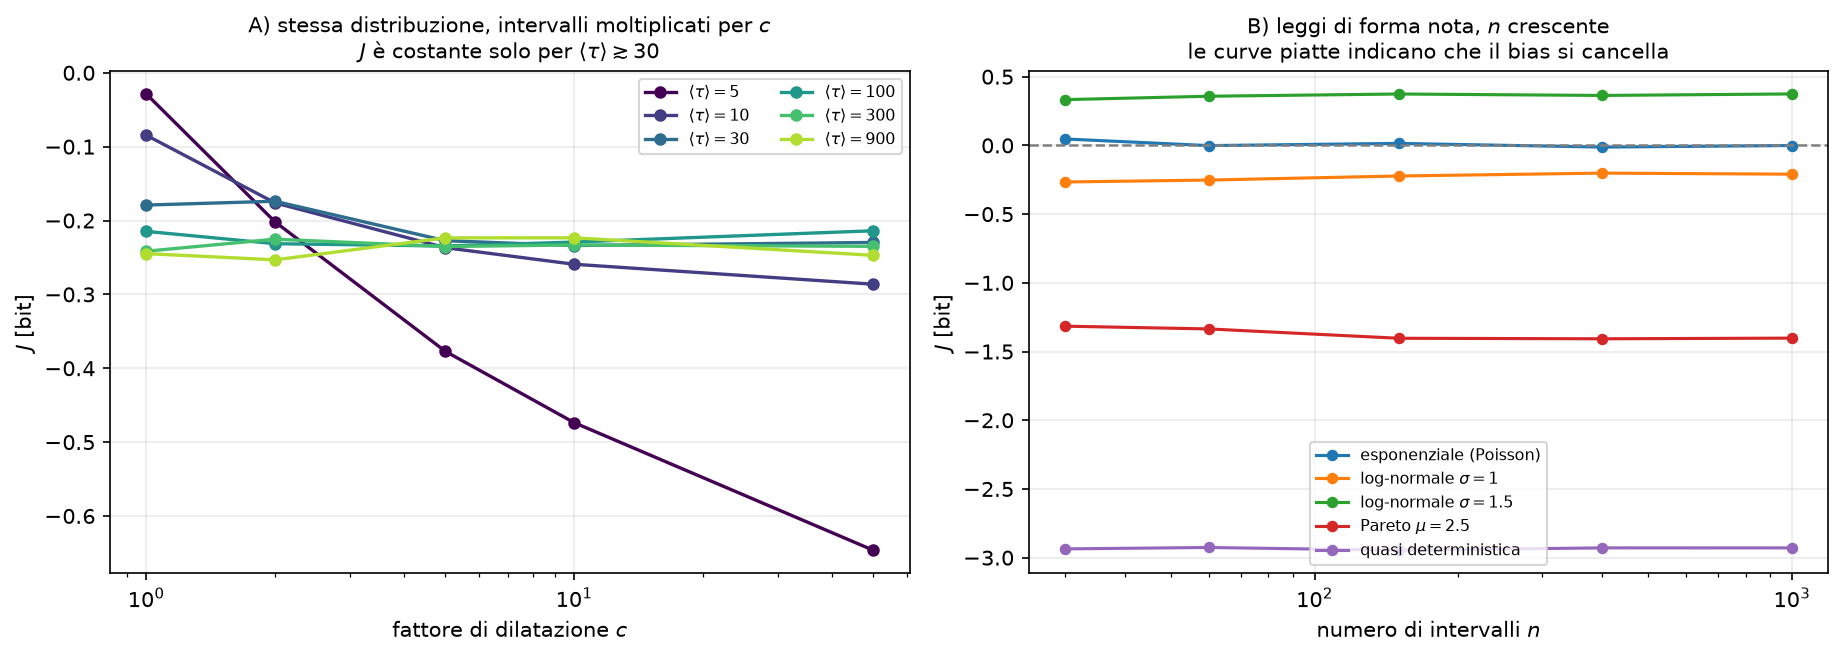
\includegraphics[width=\textwidth]{figure/cap2_invarianza_J.png}
  \caption{Limiti di validità della~\eqref{eq:entropia-intervalli}, misurati
  sullo stimatore effettivamente impiegato. A: intervalli estratti da una stessa
  legge log-normale e moltiplicati per un fattore $c$, per sei valori
  dell'intervallo medio di partenza; una curva piatta indica invarianza. Sotto
  $\langle\tau\rangle \simeq 30$ la quantizzazione agli interi la distrugge. B:
  $J$ su cinque leggi di forma nota al crescere del numero di intervalli; lo
  scostamento fra gli estremi quantifica il bias che la sottrazione del termine
  poissoniano non elimina.}
  \label{fig:invarianza-J}
\end{figure}

Valori positivi di $J$ indicano intervalli distribuiti in modo più irregolare di
un processo di Poisson, valori negativi una regolarità superiore a quella del
caso. La quantità non compare in nessuno dei lavori di riferimento ed è
introdotta qui; il §\ref{sec:entropia-intervalli} ne verifica la stabilità
rispetto alla lunghezza di analisi e la impiega per neutralizzare l'effetto
appena descritto.


% ---------------------------------------------------------------------
\section{Entropia e compressione}
\label{sec:entropia}

Il concetto di disordine di un testo e la nozione di entropia sono già stati
introdotti nel Capitolo~\ref{cap:introduzione}. Trattandosi di un concetto
centrale per questo lavoro, in questa sezione viene definito in modo formale e
ne viene esplicitato il legame con gli algoritmi di compressione, che è lo
strumento con cui l'entropia verrà effettivamente stimata sui testi.

% ---------------------------------------------------------------------
\subsection{Entropia e predicibilità}
\label{sec:entropia-def}

Si consideri una sorgente che emette simboli da un alfabeto finito
$\mathcal{X}$. Per una singola variabile aleatoria $X$ che assume il valore
$x \in \mathcal{X}$ con probabilità $p(x)$, l'entropia di
Shannon~\cite{shannon1948} è
\begin{equation}
  H(X) \;=\; -\sum_{x \in \mathcal{X}} p(x) \log_2 p(x),
  \label{eq:H-singola}
\end{equation}
espressa in bit, e misura l'incertezza media sull'esito dell'estrazione.

I simboli di un testo non sono però indipendenti, e l'entropia di una singola
lettera non descrive la sorgente: sapere che in inglese la lettera più frequente
è \emph{e} dice poco, mentre sapere che dopo \emph{th} segue quasi sempre
\emph{e} dice molto. Occorre quindi considerare blocchi di simboli. Detta
$H(X_1,\dots,X_n)$ l'entropia congiunta di un blocco di lunghezza $n$, definita
dalla~\eqref{eq:H-singola} applicata alla distribuzione congiunta dei blocchi, si
definisce il tasso di entropia della sorgente come
\begin{equation}
  h \;=\; \lim_{n\to\infty} \frac{H(X_1,\dots,X_n)}{n} .
  \label{eq:tasso-entropia}
\end{equation}
Il limite esiste per sorgenti stazionarie ed ergodiche~\cite{cover2006} e
quantifica l'incertezza media per simbolo una volta tenuto conto di tutte le
dipendenze, comprese quelle a lunga distanza. È questa, e non
la~\eqref{eq:H-singola}, la quantità pertinente per un testo.

Il teorema della codifica di sorgente~\cite{cover2006} lega $h$ alla
comprimibilità: il tasso di entropia è un limite inferiore alla lunghezza media
per simbolo di qualunque codifica senza perdita. Stimare l'entropia di un testo
e stimarne la comprimibilità sono quindi, entro le approssimazioni del caso, lo
stesso problema.

Il legame si comprende in modo intuitivo tornando ai casi limite della
Tabella~\ref{tab:tre-regimi}. Un algoritmo di compressione senza perdita opera
sostituendo alle porzioni di testo che si ripetono un riferimento
all'occorrenza precedente, più breve del testo che rimpiazza. Nel testo monotono
il medesimo gruppo di parole ricorre per l'intera lunghezza del documento: dopo
la prima occorrenza tutto il resto è un riferimento, il file compresso è
minuscolo e il tasso di entropia è prossimo a zero, perché il simbolo successivo
è quasi sempre determinato da quelli che lo precedono. Nella sequenza casuale,
al contrario, nessuna porzione si ripete: non esiste nulla cui fare riferimento,
il compressore non guadagna nulla e il tasso di entropia è massimo, perché ogni
simbolo è imprevedibile a partire dai precedenti. Il linguaggio naturale si
colloca fra i due estremi, e la quantità di compressione che ammette è una
misura diretta di quanta struttura possiede.

\paragraph{Stimatori di Lempel--Ziv.}
La stima diretta di $h$ dalla~\eqref{eq:tasso-entropia} per conteggio di blocchi
è impraticabile: il numero di blocchi distinti di lunghezza $n$ cresce
esponenzialmente con $n$, e la dimensione campionaria necessaria a stimarne le
probabilità cresce di conseguenza. Nessun testo reale è abbastanza lungo.

Si ricorre allora agli stimatori della famiglia Lempel--Ziv~\cite{ziv1977},
che aggirano il problema misurando le ripetizioni invece delle probabilità.
L'idea è la seguente: si scorre la successione e, a ogni posizione $i$, si cerca
la più lunga sottostringa che inizi in $i$ e sia già comparsa in precedenza,
detta $\Lambda_i$ la sua lunghezza. In un testo molto ripetitivo i match sono
lunghi, in un testo casuale sono corti. Si dimostra che, per una sorgente
stazionaria ed ergodica, la lunghezza media di tali match cresce come il
logaritmo della finestra esplorata e che
\begin{equation}
  h \;=\; \lim_{n\to\infty}
  \left\langle \frac{\log_2 n}{\Lambda_i} \right\rangle ,
  \label{eq:lz-entropia}
\end{equation}
dove la media è presa sulle posizioni $i$. La~\eqref{eq:lz-entropia} converge
assai più rapidamente del conteggio di blocchi e mantiene buone proprietà anche
in presenza di correlazioni a lungo raggio, che è la ragione per cui viene
adottata qui: le sorgenti considerate in questa tesi hanno, per costruzione,
memoria lunga.

% ---------------------------------------------------------------------
\subsection{Stima della cross-entropia e della divergenza}
\label{sec:crossparsing}

Le quantità introdotte finora descrivono un testo singolo. Per confrontare due
testi occorre la cross-entropia, che misura il costo di codificare un testo
usando la statistica di un altro.

L'algoritmo di cross-parsing di Ziv e Merhav~\cite{ziv1993} estende
la~\eqref{eq:lz-entropia} a due successioni. Data la successione $x$ da
misurare e la successione di riferimento $y$, si scorre $x$ da sinistra a destra
e la si decompone in frasi successive, dove ogni frase è la più lunga
sottostringa che, a partire dalla posizione corrente, compaia da qualche parte
in $y$; raggiunto il punto in cui il match si interrompe, si chiude la frase e
se ne apre una nuova. Il numero di frasi così ottenute viene indicato con
$c(x|y)$ ed è la quantità che misura la somiglianza fra i due testi: se $x$ e
$y$ provengono dalla stessa sorgente, le frasi sono lunghe e poche; se
provengono da sorgenti diverse, i match si interrompono presto e le frasi sono
molte. La stima della cross-entropia è
\begin{equation}
  h(x \,|\, y) \;=\; \frac{c(x|y)\,\log_2 |y|}{|x|},
  \label{eq:crossparsing}
\end{equation}
espressa in bit per simbolo, dove $|x|$ e $|y|$ sono le lunghezze delle due
successioni.

La divergenza di Kullback--Leibler è lo strumento con cui si quantifica quanto
due distribuzioni di probabilità differiscano fra loro. Date due distribuzioni
$P$ e $Q$ sullo stesso alfabeto, essa è definita come
\begin{equation}
  D(P\|Q) \;=\; \sum_{x} P(x) \log_2 \frac{P(x)}{Q(x)}
  \;=\; H_P(Q) - H(P),
  \label{eq:kl-def}
\end{equation}
dove $H_P(Q)$ è la cross-entropia fra le due distribuzioni. La~\eqref{eq:kl-def}
si interpreta come il numero medio di bit sprecati per simbolo codificando una
sorgente $P$ con un codice ottimizzato per $Q$: vale zero se e solo se
$P = Q$ ed è positiva altrimenti.

In termini di successioni, la~\eqref{eq:kl-def} si stima come differenza fra due
cross-entropie: dividendo $x$ in due metà $x_1$ e $x_2$ e prendendo da $y$ un
prefisso $y_1$ della stessa lunghezza di $x_1$, si pone
\begin{equation}
  D(x \,\|\, y) \;=\; h(x_2 \,|\, y_1) \;-\; h(x_2 \,|\, x_1) .
  \label{eq:kl}
\end{equation}
La seconda metà di $x$ viene cioè codificata due volte, una volta usando come
riferimento un testo estraneo e una volta usando la prima metà di $x$ stesso, e
si misura quanto costa in più la prima operazione.

L'appaiamento delle lunghezze dei due riferimenti non è un dettaglio.
La~\eqref{eq:crossparsing} dipende dalla lunghezza del riferimento, poiché un
riferimento più lungo contiene più sottostringhe e produce una cross-entropia
minore a parità di sorgente. Se i due termini della~\eqref{eq:kl} usassero
riferimenti di lunghezza diversa, la differenza conterrebbe un termine spurio
che può superare in modulo il segnale da misurare e produrre stime negative,
impossibili per la~\eqref{eq:kl-def}. Con $|y_1| = |x_1|$ il termine spurio si
cancella, e la costruzione soddisfa la proprietà verificabile $D(x\|x) = 0$
esattamente, impiegata nei capitoli sperimentali come test dello stimatore.

Poiché la~\eqref{eq:kl} non è simmetrica, mentre per confrontare due corpora
serve una quantità che non dipenda da quale dei due venga posto come
riferimento, seguendo~\cite{lippi2019} viene adottata la divergenza
simmetrizzata
\begin{equation}
  D_s(x,y) \;=\; \tfrac{1}{2}\bigl[D(x\|y) + D(y\|x)\bigr].
  \label{eq:kl-sym}
\end{equation}

% ---------------------------------------------------------------------
\subsection{Misure basate su compressione}
\label{sec:compressione}

Le stime della sottosezione precedente usano la compressione come strumento
teorico, attraverso il conteggio delle frasi. Un secondo gruppo di misure,
introdotto in questo contesto da Hadad et al.~\cite{hadad2026}, impiega invece
direttamente un compressore reale come sonda della regolarità strutturale, senza
passare per una stima di entropia.

Detta $C(x)$ la dimensione in byte del testo $x$ dopo la compressione, si
definisce il rapporto di compressione
\begin{equation}
  R_{\mathrm{gzip}}(x) \;=\; \frac{C(x)}{|x|},
  \label{eq:cratio}
\end{equation}
tanto minore quanto più il testo è regolare. Il pedice ricorda l'algoritmo
impiegato e distingue la quantità dal descrittore $R$ della~\eqref{eq:R}.

Da esso derivano la compressione condizionata
$\bigl(C(x+y) - C(x)\bigr)/|y|$, dove $x+y$ indica la concatenazione, che stima
il costo incrementale di codificare la seconda metà di un documento dopo aver
già codificato la prima e misura quindi quanto la seconda metà sia prevedibile
a partire dalla prima; e la distanza normalizzata di compressione~\cite{li2004}
\begin{equation}
  \mathrm{NCD}(x,y) \;=\;
  \frac{C(xy) - \min\{C(x),C(y)\}}{\max\{C(x),C(y)\}} .
  \label{eq:ncd}
\end{equation}
Applicata fra un testo e una sua permutazione, la~\eqref{eq:ncd} misura quanta
parte della comprimibilità dipenda dall'ordine delle parole e non dalla sola
composizione lessicale: è quindi l'analogo, in chiave di compressione, del
confronto fra i pannelli della Figura~\ref{fig:barcode}.


% ---------------------------------------------------------------------
\section{Token ed embedding}
\label{sec:token}

Nel §\ref{sec:scala} si è assunta la parola come unità fondamentale del testo,
in quanto più piccola porzione dotata di significato autonomo per un lettore
umano. Questa scelta non vale più per gli algoritmi di generazione automatica
del testo e, in particolare, per i modelli linguistici di grandi dimensioni.

Si riprenda la frase già usata come esempio,
\emph{Se pensi di comprendere la meccanica quantistica, non comprendi la
meccanica quantistica.} Per un lettore umano essa si scompone come nella
Figura~\ref{fig:scomp-parole}: dodici parole più la punteggiatura, ciascuna
delle quali ha un significato che si può cercare in un dizionario.

\begin{figure}[htbp]
  \centering
  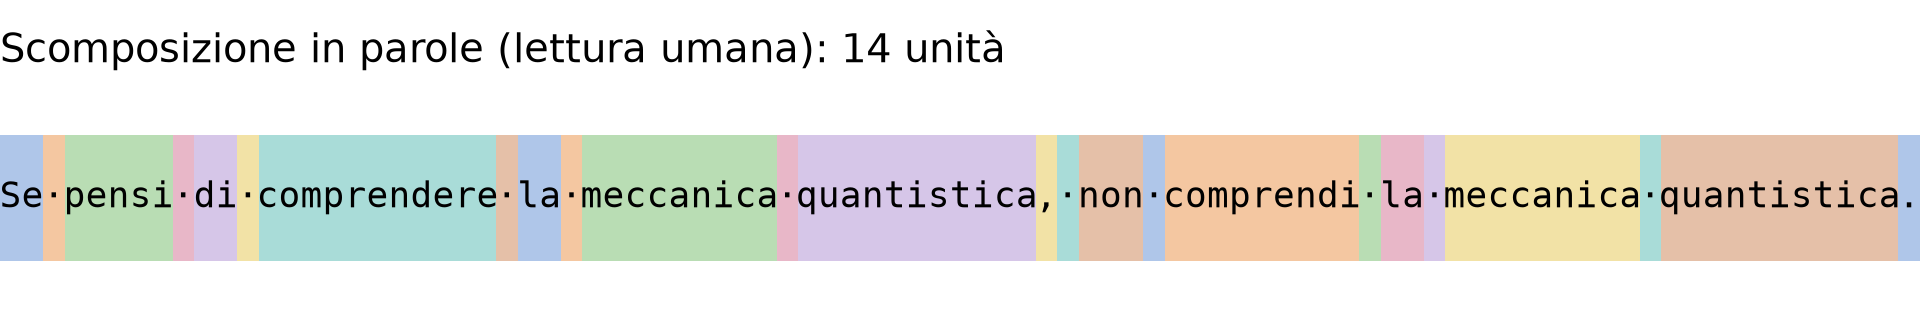
\includegraphics[width=\textwidth]{figure/cap2_scomposizione_parole.png}
  \caption{Scomposizione in parole. Ogni blocco è un'unità dotata di
  significato autonomo; il punto mediano segnala gli spazi.}
  \label{fig:scomp-parole}
\end{figure}

Per un modello linguistico la stessa frase si scompone invece come nella
Figura~\ref{fig:scomp-token}.

\begin{figure}[htbp]
  \centering
  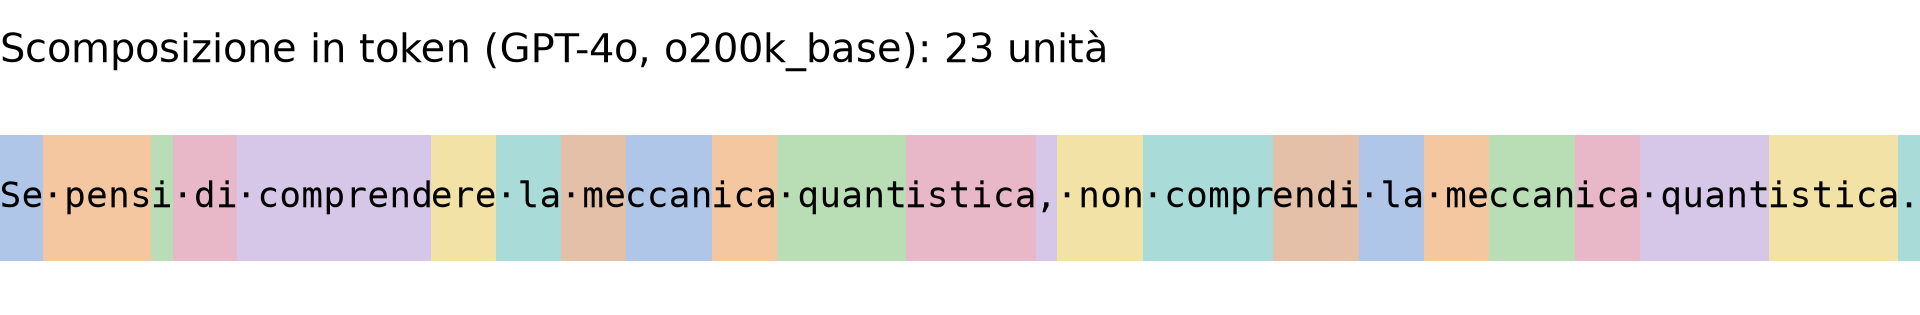
\includegraphics[width=\textwidth]{figure/cap2_scomposizione_token.png}
  \caption{Scomposizione in token della stessa frase, ottenuta con il
  tokenizzatore \texttt{o200k\_base} impiegato da GPT-4o. Le unità sono
  ventitré, non coincidono con le parole e in generale non hanno significato
  autonomo.}
  \label{fig:scomp-token}
\end{figure}

La frase non è divisa né in lettere né in parole, ma in gruppi di lettere
chiamati \emph{token}. Alcuni token coincidono con parole intere
(\texttt{·la}, \texttt{·non}), altri sono frammenti privi di significato
(\texttt{ccan}, \texttt{istica}). Si osservi in particolare la coppia
\emph{comprendere} e \emph{comprendi}: la prima si scompone in
\texttt{·comprend} e \texttt{ere}, la seconda in \texttt{·compr} e
\texttt{endi}. Due forme della stessa radice vengono dunque tagliate in punti
diversi, e il modello non riceve alcuna indicazione esplicita del fatto che
condividano la radice. Lo spazio, inoltre, non separa i token ma vi è
incorporato: la maggior parte dei token inizia con uno spazio, e la
segmentazione del testo in unità precede logicamente qualunque nozione di
parola.

La conversione avviene tramite un algoritmo detto \emph{tokenizzatore}, che
traduce un testo scritto in una qualsiasi lingua e in un qualsiasi alfabeto in
una sequenza di token estratti da un dizionario ampio ma finito, costruito una
volta per tutte a partire da un grande corpus. I dizionari dei tokenizzatori
più diffusi hanno dimensioni dell'ordine di $10^5$ elementi: quello di GPT-4o,
\texttt{o200k\_base}, ne conta \num{200019}; \texttt{cl100k\_base}, impiegato
come unità di analisi nei capitoli sperimentali per le ragioni discusse nel
Capitolo~\ref{cap:metodi}, ne conta \num{100277}; i modelli Qwen2.5 analizzati
in questa tesi ne condividono uno di circa \num{151000} voci. Poiché il
dizionario è finito ma le lingue possibili sono molte, i testi nelle lingue
meno rappresentate nel corpus di costruzione vengono frammentati in un numero
di token assai maggiore rispetto all'inglese.

Proprio come le parole per gli esseri umani, per un modello linguistico sono i
token a trasportare significato. Il significato non è però un'etichetta
associata al token, bensì una posizione: tramite un'operazione detta
\emph{embedding} ogni token viene mappato in un vettore di uno spazio a molte
dimensioni, e la geometria di quello spazio codifica le relazioni fra i token.
Vettori vicini corrispondono a token che compaiono in contesti simili, e
direzioni ricorrenti nello spazio corrispondono a relazioni ricorrenti nel
linguaggio.

La Figura~\ref{fig:embedding} mostra la proprietà su un caso concreto. I vettori
di trenta parole inglesi, appartenenti a cinque famiglie semantiche, sono
proiettati sulle prime due componenti principali dello spazio: le parole di
ciascuna famiglia si dispongono in gruppi distinti, benché la costruzione dei
vettori non abbia mai fatto uso di alcuna classificazione semantica, ma soltanto
delle co-occorrenze osservate in un corpus.

\begin{figure}[htbp]
  \centering
  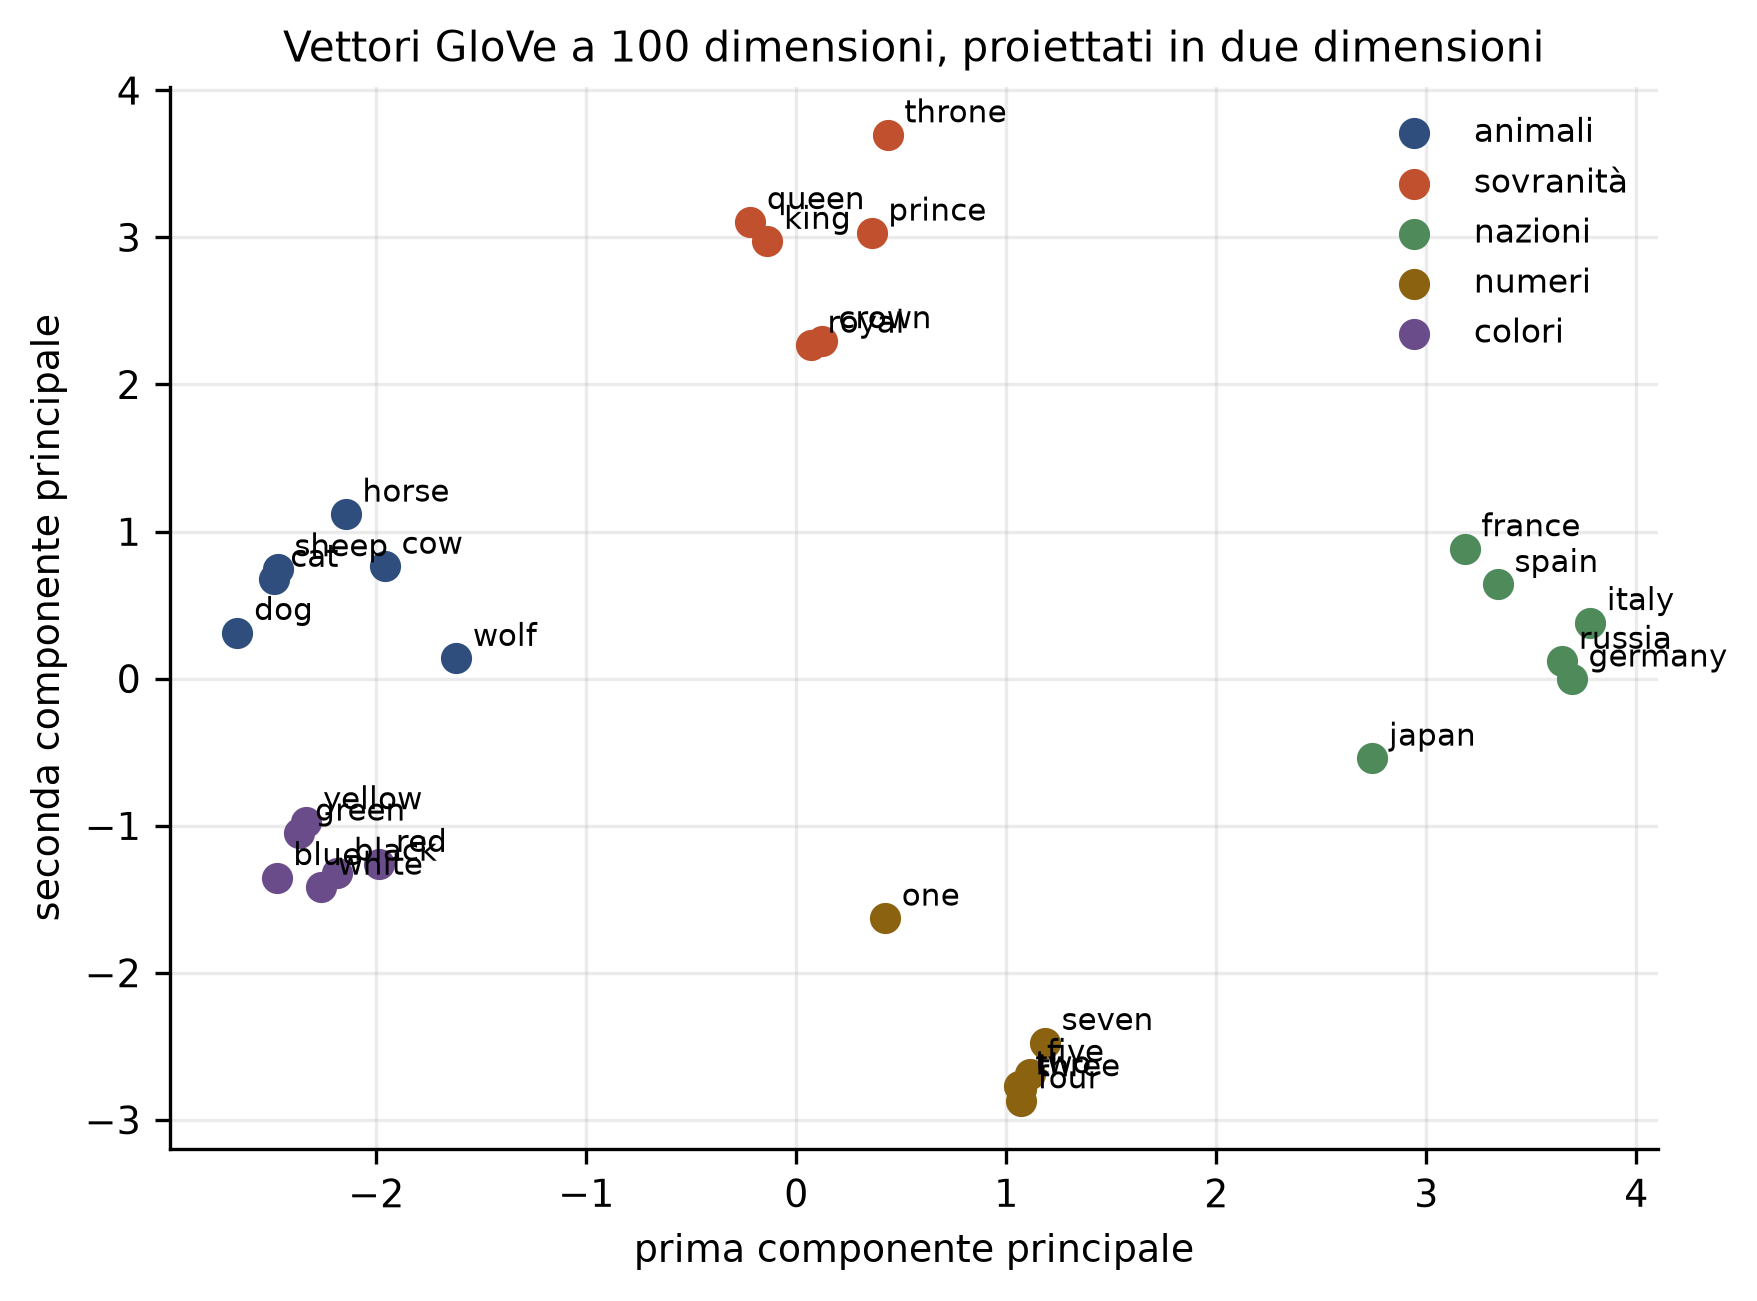
\includegraphics[width=0.82\textwidth]{figure/cap2_embedding_2d.png}
  \caption{Trenta parole inglesi rappresentate dai rispettivi vettori GloVe a
  100 dimensioni, proiettati sulle prime due componenti principali. Le cinque
  famiglie semantiche formano gruppi separati senza che alcuna informazione
  semantica sia stata fornita all'algoritmo. La proiezione conserva soltanto una
  parte della struttura, poiché riduce cento dimensioni a due: la vicinanza
  visibile in figura è una condizione sufficiente, non necessaria, alla
  vicinanza nello spazio originario.}
  \label{fig:embedding}
\end{figure}

I due spazi vettoriali che compaiono in questo lavoro hanno natura diversa. Ogni modello linguistico possiede una propria matrice di embedding,
appresa durante l'addestramento insieme a tutti gli altri parametri, e i cui
vettori non sono direttamente confrontabili fra modelli diversi: fra i modelli
analizzati in questa tesi la dimensione di tale spazio passa da 1536 per il
modello da 1.5 miliardi di parametri a 5120 per quello da 14 miliardi. Gli embedding impiegati nelle analisi di
questa tesi sono invece vettori GloVe a 100 dimensioni, pre-addestrati su un
corpus esterno e identici per tutti i testi esaminati: la scelta è dettata dalla
necessità di misurare i testi generati da modelli diversi con lo stesso metro, e
segue l'impostazione di~\cite{mikhaylovskiy2025states}. Nel
§\ref{sec:traiettoria} tali vettori verranno usati per trasformare un testo in
una traiettoria nello spazio semantico e studiarne l'autocorrelazione.


% ---------------------------------------------------------------------
\section{Generazione autoregressiva e temperatura}
\label{sec:temperatura}

Un modello linguistico autoregressivo, data una sequenza di token $t_{1:m}$,
sceglie il token successivo estraendolo da una distribuzione di probabilità che
dipende dalla sequenza stessa. La probabilità dell'intera sequenza si
decompone per mezzo della regola della catena,
\begin{equation}
  P(t_{1:m}) \;=\; \prod_{k=1}^{m} P(t_k \mid t_{1:k-1}),
  \label{eq:autoregressivo}
\end{equation}
e il modello è addestrato ad approssimare i singoli fattori
$P(t_k \mid t_{1:k-1})$, cioè a prevedere ogni token a partire da tutti quelli
che lo precedono. La generazione consiste nell'applicare ripetutamente questa
previsione, aggiungendo di volta in volta il token estratto alla sequenza che
condiziona l'estrazione successiva.

\paragraph{Origine della distribuzione condizionata.}
Il modo in cui il modello costruisce $P(t_k \mid t_{1:k-1})$ è ciò che
distingue le architetture moderne da quelle precedenti, ed è rilevante per
questo lavoro. I modelli oggi in uso si basano sull'architettura
\emph{transformer}~\cite{vaswani2017}, il cui elemento caratteristico è il
meccanismo di \emph{attenzione}. In esso ogni posizione della sequenza calcola
un peso per ciascuna delle posizioni precedenti e costruisce la propria
rappresentazione come combinazione pesata di quelle: il token in posizione $k$
può quindi attingere direttamente a qualunque token precedente, per lontano che
sia, senza che l'informazione debba propagarsi attraverso le posizioni
intermedie.

È una differenza sostanziale rispetto ai modelli ricorrenti, in cui
l'informazione proveniente da una posizione lontana deve attraversare tutte
quelle interposte e si degrada di conseguenza. Nel transformer il cammino fra
due posizioni qualsiasi ha lunghezza costante, e questo rende l'architettura in
linea di principio capace di rappresentare dipendenze fra porzioni di testo
molto distanti fra loro. È il meccanismo che, negli attuali modelli, potrebbe
dare origine alle correlazioni a lungo raggio descritte nel §\ref{sec:lrc}, e
una delle ragioni per cui ha senso cercarle nel testo generato. La capacità di
rappresentare tali dipendenze non implica però che il modello le riproduca
effettivamente, e l'attenzione opera comunque entro una finestra di contesto
finita: stabilire se le correlazioni siano presenti nel
testo prodotto resta una questione empirica, ed è precisamente quella affrontata
nei capitoli sperimentali.

\paragraph{Temperatura.}
Il modello non produce direttamente probabilità, ma valori reali detti
\emph{logit}, indicati con $u_1,\dots,u_{|\mathcal{L}|}$, uno per ciascun
elemento del dizionario $\mathcal{L}$. Essi vengono convertiti in distribuzione
di probabilità da una funzione softmax riscalata da un parametro
$T$~\cite{ackley1985}:
\begin{equation}
  p(t = \mathcal{L}_l \mid t_{1:i-1}) \;=\;
  \frac{\exp(u_l / T)}{\sum_{l'} \exp(u_{l'} / T)} .
  \label{eq:softmax}
\end{equation}

Il parametro $T$ prende il nome di temperatura, e la denominazione non è una
semplice analogia. Ponendo $E_l = -u_l$, la~\eqref{eq:softmax} coincide con la
distribuzione di Boltzmann $p_l \propto e^{-E_l/T}$ di un sistema a
$|\mathcal{L}|$ stati in equilibrio termico alla temperatura $T$. Questa
identificazione è ciò che giustifica la ricerca, nel testo generato, dei
fenomeni caratteristici dei sistemi termodinamici, e in particolare delle
transizioni di fase discusse nel §\ref{sec:fasi}.

I due limiti sono immediati. Per $T\to0$ la distribuzione si concentra sul token
di logit massimo e la generazione diventa deterministica; per $T\to\infty$ tende
alla distribuzione uniforme sull'intero dizionario, indipendentemente dal
contesto. Fra i due estremi, valori $T<1$ concentrano la massa di probabilità
sugli eventi più probabili, mentre valori $T>1$ la ridistribuiscono verso quelli
meno probabili. La temperatura non modifica dunque ciò che il modello ha
appreso, ma soltanto quanto fedelmente la generazione segue la distribuzione
appresa.

Nella pratica corrente la generazione impiega anche il troncamento della
distribuzione, nelle varianti top-$k$~\cite{fan2018} e
top-$p$~\cite{holtzman2020}, e penalità che scoraggiano la ripetizione. Tutti
questi meccanismi agiscono sulla stessa distribuzione e introducono un secondo
parametro d'ordine, rendendo impossibile attribuire alla sola temperatura il
comportamento osservato. Per questa ragione, e coerentemente con la scelta
esplicita di~\cite{mikhaylovskiy2025zipf}, i dati analizzati in questa tesi sono
stati generati impiegando il solo campionamento per temperatura.


% ---------------------------------------------------------------------
\section{Fasi e stato critico}
\label{sec:fasi}

Una fase di un sistema fisico è uno stato, tipicamente di equilibrio, dotato di
proprietà macroscopiche caratteristiche e stabile in una regione dello spazio
dei parametri; alla frontiera di tali regioni avviene una transizione di fase.
Secondo la classificazione di Ehrenfest~\cite{ehrenfest1933} una transizione di
ordine $n$ è una discontinuità nella derivata $n$-esima dell'energia libera.

Applicare alla lettera questa classificazione al testo generato non è però
possibile. Il sistema considerato non ha un'energia libera di cui prendere
derivate, non è in equilibrio con alcun bagno termico e
non possiede un limite termodinamico, poiché il numero di token di un documento
resta finito. Ciò che rende legittimo il linguaggio delle fasi è la
corrispondenza stabilita nel §\ref{sec:temperatura}: la~\eqref{eq:softmax}
coincide con una distribuzione di Boltzmann in cui i logit giocano il ruolo di
energie e il parametro di campionamento quello di temperatura. La distribuzione
condizionata da cui ogni token viene estratto è dunque, letteralmente, una
distribuzione di Gibbs, e $T$ ne è la temperatura. Quello che resta analogia, e
non identità, è il passaggio dal singolo token al documento: nulla garantisce
che le proprietà collettive di una sequenza generata token per token si
comportino come le proprietà macroscopiche di un sistema all'equilibrio. Il
vocabolario di Ehrenfest viene perciò impiegato in senso descrittivo, per
nominare regioni di comportamento qualitativamente diverso separate da
variazioni rapide, e non per rivendicare una transizione di fase in senso
termodinamico.

Ciò che rende il concetto utile è il comportamento nel punto critico che
separa due fasi: là le correlazioni decadono a legge di potenza e la loro
portata diverge, e molte grandezze osservabili esibiscono lo stesso andamento.
Il criterio inverso, per cui dove compare una legge di potenza si sospetta uno
stato critico, va maneggiato con prudenza, perché distribuzioni a legge di
potenza si generano in molti modi che con la criticità non hanno rapporto, dal
semplice prodotto di variabili aleatorie ai processi di preferential
attachment. Preso da solo, l'andamento a legge di potenza di una quantità non
dimostra nulla. Acquista forza quando più osservabili indipendenti cambiano
regime allo stesso valore del parametro di controllo, ed è in questa forma che
viene impiegato nel §\ref{sec:tstar}: non la legge di potenza di una misura,
ma la convergenza di criteri costruiti per scopi diversi.

Il quadro è stato applicato ai modelli linguistici in~\cite{nakaishi2024}, dove
la temperatura di campionamento separa una fase a bassa temperatura,
caratterizzata da strutture ripetitive, da una ad alta temperatura in cui il
testo è incomprensibile. La tesi sostenuta in quel lavoro è che il linguaggio
naturale si collochi \emph{sul} punto critico fra le due: nello spazio dei
processi stocastici che generano successioni di simboli, il processo
corrispondente a una lingua naturale giacerebbe sulla superficie critica che
separa le due regioni, e un modello addestrato su quella lingua definisce una
famiglia di processi che quella superficie attraversa al variare di $T$. Il
risultato è verificato su modelli da 160 milioni a 2.8 miliardi di parametri, su
sei lingue e su due diverse mappature del testo in successione numerica, il che
ne stabilisce l'indipendenza dalla scala e dalla lingua.

Questa congettura è il punto di contatto più stretto fra il presente lavoro e la
letteratura di fisica statistica sull'argomento, e il
Capitolo~\ref{cap:risultati1} ne fornisce una verifica indipendente: se il
linguaggio naturale è critico, allora la temperatura alla quale il testo
generato somiglia di più a quello umano deve coincidere con quella alla quale il
modello attraversa la transizione, e criteri che misurano proprietà diverse
devono indicarla concordemente.


% ---------------------------------------------------------------------
\subsection{La traiettoria di embedding}
\label{sec:traiettoria}

Il §\ref{sec:token} ha introdotto i vettori di embedding come rappresentazione
del significato. Applicandoli a un testo si ottiene un oggetto geometrico: detta
$(p_1,\dots,p_M)$ la successione delle parole del documento e $v(\cdot)$ la
mappa che associa a una parola il proprio vettore, si pone
\begin{equation}
  \mathbf{m}_i \;=\;
  \begin{cases}
    v(p_i) - \bar{v} & \text{se $p_i$ ha un vettore},\\[2pt]
    \mathbf{0}       & \text{altrimenti},
  \end{cases}
  \label{eq:traiettoria}
\end{equation}
dove $\bar{v}$ è la media dei vettori delle sole parole che ne possiedono uno.
La successione $(\mathbf{m}_1,\dots,\mathbf{m}_M)$ è la traiettoria del testo
nello spazio degli embedding: ogni parola è un punto, e leggere il documento
dall'inizio alla fine equivale a percorrere quella traiettoria.

Due dettagli della~\eqref{eq:traiettoria} incidono sui risultati. Il primo è la
centratura: sottrarre $\bar{v}$ elimina la
direzione media del documento, che altrimenti dominerebbe ogni prodotto scalare
e renderebbe tutte le coppie di parole artificialmente simili. Il secondo è il
trattamento delle parole prive di vettore, alle quali si assegna il vettore
nullo \emph{dopo} la centratura, seguendo~\cite{mikhaylovskiy2025states}: la
posizione nella successione viene così conservata, e con essa la struttura dei
lag, ma la parola non contribuisce ad alcuna correlazione. La conseguenza è che
un testo in cui molte parole non hanno vettore produce una traiettoria fatta in
larga parte di zeri, e le misure che seguono perdono significato prima di
diventare incalcolabili: è la ragione della soglia di validità introdotta più
avanti.

Su questa successione si definisce l'autocorrelazione a distanza $\tau$ come
media della similarità coseno fra i vettori che distano $\tau$ posizioni,
\begin{equation}
  C(\tau) \;=\; \frac{1}{M-\tau} \sum_{i=1}^{M-\tau}
  \frac{\mathbf{m}_i \cdot \mathbf{m}_{i+\tau}}
       {\lVert \mathbf{m}_i \rVert \, \lVert \mathbf{m}_{i+\tau} \rVert},
  \label{eq:acf-embedding}
\end{equation}
con la convenzione che i termini in cui uno dei due vettori è nullo
contribuiscono zero. La~\eqref{eq:acf-embedding} risponde alla domanda: due
parole che distano $\tau$ posizioni tendono a essere semanticamente affini? Vale
$C(\tau) \simeq 0$ quando non c'è alcuna relazione, ed è tanto più vicina a uno
quanto più il testo, a quella distanza, torna a parlare della stessa cosa.

Poiché la~\eqref{eq:acf-embedding} resta calcolabile su qualunque successione,
serve un riferimento che dica quale ampiezza sia distinguibile dal caso. Si
adotta il rimescolamento: si permutano a caso le posizioni della traiettoria, si
ricalcola $C(\tau)$ e si prende il massimo del suo modulo. Il valore così
ottenuto è il livello di rumore del documento, ed è la stessa costruzione dei
null model del §\ref{sec:null}: conserva il contenuto e distrugge l'ordine.
Un'autocorrelazione la cui ampiezza non superi quel livello non è distinguibile
da una successione di parole senza struttura.


% ---------------------------------------------------------------------
\subsection{Le tre fasi}
\label{sec:tre-fasi}

Applicando questo linguaggio al testo generato,
in~\cite{mikhaylovskiy2025states} vengono individuate tre fasi, distinte dal
comportamento di $C(\tau)$.

A bassa temperatura il testo degenera in cicli di ripetizione: la traiettoria
ripassa periodicamente per gli stessi punti, $C(\tau)$ oscilla con periodo pari
alla lunghezza del ciclo e la sua trasformata di Fourier presenta picchi netti.
La quantità che segnala il fenomeno è quindi
\begin{equation}
  \Phi \;=\; \max_{k \ge 1} \bigl\lvert \hat{C}_k \bigr\rvert ,
  \label{eq:periodicita}
\end{equation}
dove $\hat{C}_k$ sono i coefficienti della trasformata discreta di $C(\tau)$. Il
coefficiente $k = 0$ viene escluso perché proporzionale alla media di $C(\tau)$,
cioè al livello complessivo di correlazione e non alla sua periodicità: un testo
uniformemente correlato ma non ciclico ha $\hat{C}_0$ grande e tutti gli altri
coefficienti piccoli. Questa è la fase che, per analogia con gli stati della
materia, viene detta solida. È lo stesso regime in cui, come osservato nel
§\ref{sec:ponte}, la fluttuazione della DFA satura e $\alpha_{\mathrm{DFA}}$
scende verso zero: le due misure segnalano lo stesso fenomeno da due angolazioni
diverse.

La~\eqref{eq:periodicita} si comporta come un parametro d'ordine nel senso che
assume valori grandi in una fase e piccoli nell'altra, ma non si annulla
identicamente fuori dalla fase periodica: su una successione priva di struttura
resta un valore residuo dovuto alle fluttuazioni campionarie. Il
Capitolo~\ref{cap:risultati1} riporta di conseguenza il suo crollo in termini di
ordini di grandezza e non di annullamento.

In una finestra ristretta di temperature $C(\tau)$ decade invece a legge di
potenza: è lo stato critico, quello in cui le leggi di Zipf e di Heaps
introdotte nel §\ref{sec:scala} risultano meglio soddisfatte. Ad alta
temperatura, infine, le correlazioni decadono esponenzialmente e non sussiste
struttura a lungo raggio: è la fase detta amorfa, o gassosa.

Per distinguere le ultime due fasi vengono confrontati due fit
dell'autocorrelazione, uno a legge di potenza e uno esponenziale, tramite il
rapporto dei rispettivi errori~\cite{mikhaylovskiy2023}:
\begin{equation}
  \mathrm{GAPELMAPER} \;=\;
  \frac{\mathrm{MAPE}\bigl(\text{fit a legge di potenza}\bigr)}
       {\mathrm{MAPE}\bigl(\text{fit esponenziale}\bigr)},
  \label{eq:gapelmaper}
\end{equation}
dove il MAPE è quello definito nella~\eqref{eq:mape}. Il rapporto è minore di 1
quando il fit a legge di potenza descrive i dati meglio di quello esponenziale,
e segnala quindi lo stato critico; è maggiore di 1 nella fase amorfa.

La~\eqref{eq:gapelmaper} è un rapporto fra errori di fit, e come tale resta
calcolabile anche quando l'autocorrelazione è indistinguibile dal rumore; in
quel regime, però, il suo valore è privo di contenuto informativo, perché
entrambi i fit descrivono male dati che non contengono alcun segnale.

Le tre fasi, la soglia di periodicità e la condizione di validità si compongono
nella regola seguente. Detti $\kappa$ la quota di parole del documento dotate di
un vettore, $A = \max_\tau \lvert C(\tau)\rvert$ l'ampiezza
dell'autocorrelazione e $\eta$ il livello di rumore stimato per rimescolamento,
un documento viene classificato come
%
\begin{itemize}
  \item \emph{non valutabile}, se $\kappa < \kappa_{\min}$ oppure $A \le \eta$;
  \item \emph{solido}, altrimenti, se $\Phi > \Phi_{\min}$;
  \item \emph{critico}, altrimenti, se $\mathrm{GAPELMAPER} < 1$;
  \item \emph{amorfo} in ogni altro caso.
\end{itemize}
%
L'ordine dei controlli non è indifferente. La condizione di validità viene per
prima perché le altre due misure, su un documento che non la supera, sono numeri
senza referente; la periodicità viene prima del GAPELMAPER perché
un'autocorrelazione periodica non è né una legge di potenza né un esponenziale,
e sottoporla a quel confronto restituirebbe un valore arbitrario. I due valori
di soglia sono fissati nel Capitolo~\ref{cap:risultati1}, dove ne vengono
discussi l'origine e l'effetto.

I due quadri di riferimento non coincidono del tutto.
In~\cite{nakaishi2024} le fasi sono due e ciò che le separa è un punto critico,
cioè un insieme di misura nulla nello spazio dei parametri;
in~\cite{mikhaylovskiy2025states} lo stato critico diventa invece una fase a sé,
dotata di estensione finita. La differenza non è terminologica: nel primo caso
attraversare la transizione con uno sweep a passo finito significa quasi
certamente saltare il punto critico, nel secondo significa attraversare una
regione che si può campionare. Il Capitolo~\ref{cap:risultati1} riporta i dati
pertinenti alla questione senza pretendere di risolverla.


% ---------------------------------------------------------------------
\section{Notazione}
\label{sec:notazione}

Le grandezze introdotte in questo capitolo provengono da lavori che adottano
simboli in conflitto fra loro. La Tabella~\ref{tab:notazione} raccoglie la
notazione seguita in questa tesi, che viene mantenuta senza eccezioni nei
capitoli successivi.

\begin{table}[htbp]
\centering
\small
\begin{tabular}{@{}l>{\raggedright\arraybackslash}p{8.3cm}c@{}}
\toprule
Simbolo & Grandezza & Definita in \\
\midrule
\multicolumn{3}{@{}l}{\itshape Testo e vocabolario} \\
$\mathbf{W}$, $w_t$, $N$ & sequenza di parole, parola in posizione $t$, lunghezza & \eqref{eq:sequenza} \\
$\mathcal{D}$, $\mathcal{D}(t)$ & dizionario e dizionario parziale & §\ref{sec:scala} \\
$f(r)$, $\alpha$ & frequenza della parola di rango $r$, esponente di Zipf & \eqref{eq:zipf} \\
$\gamma_H$ & esponente di Heaps & \eqref{eq:heaps} \\
$R$ & parole nuove nella seconda metà, rapportate alla prima & \eqref{eq:R} \\
MAPE & errore percentuale assoluto medio del fit & \eqref{eq:mape} \\
\addlinespace
\multicolumn{3}{@{}l}{\itshape Correlazioni} \\
$x_k$ & successione binaria generata da un osservabile & \eqref{eq:osservabile} \\
$c(s)$, $\theta$ & autocorrelazione a distanza $s$ e suo esponente di decadimento & \eqref{eq:acf-power} \\
$X(t)$, $\sigma_X^2$, $\gamma$ & conteggio, sua varianza, esponente di crescita & \eqref{eq:sigma} \\
$F(s)$, $\alpha_{\mathrm{DFA}}$ & fluttuazione detrendizzata e suo esponente & \eqref{eq:dfa-alpha} \\
\addlinespace
\multicolumn{3}{@{}l}{\itshape Intervalli e burstiness} \\
$\tau_i$, $p(\tau)$ & intervalli fra occorrenze e loro distribuzione & §\ref{sec:burst} \\
cv, $B$ & coefficiente di variazione, indice di Goh--Barabási & \eqref{eq:cv}, \eqref{eq:goh} \\
$S(0)$, $c_\tau(k)$ & spettro a frequenza nulla, autocorrelazione degli intervalli & \eqref{eq:eq4} \\
$\hat\gamma_{A1}$, $\hat\gamma_{A2}$ & esponenti misurati sui due null model & §\ref{sec:null} \\
$q$ & quota di burstiness & \eqref{eq:quota} \\
$\mu$, $\tau_c$ & esponente di coda e cut-off di $p(\tau)$ & \eqref{eq:troncata} \\
$J$ & entropia degli intervalli, riferita al processo di Poisson & \eqref{eq:entropia-intervalli} \\
\addlinespace
\multicolumn{3}{@{}l}{\itshape Entropia e compressione} \\
$H$, $h$ & entropia di Shannon, tasso di entropia & \eqref{eq:H-singola}, \eqref{eq:tasso-entropia} \\
$c(x|y)$, $h(x|y)$ & frasi del cross-parsing, cross-entropia stimata & \eqref{eq:crossparsing} \\
$D(x\|y)$, $D_s$ & divergenza di Kullback--Leibler e sua versione simmetrizzata & \eqref{eq:kl}, \eqref{eq:kl-sym} \\
$C(x)$, $R_{\mathrm{gzip}}$ & dimensione compressa e rapporto di compressione & \eqref{eq:cratio} \\
NCD & distanza normalizzata di compressione & \eqref{eq:ncd} \\
\addlinespace
\multicolumn{3}{@{}l}{\itshape Generazione e fasi} \\
$u_l$, $T$ & logit del token $l$, temperatura di campionamento & \eqref{eq:softmax} \\
$C(\tau)$ & autocorrelazione della traiettoria di embedding & \eqref{eq:acf-embedding} \\
$\Phi$ & parametro di periodicità di $C(\tau)$ & \eqref{eq:periodicita} \\
GAPELMAPER & rapporto fra gli errori dei due fit dell'autocorrelazione & \eqref{eq:gapelmaper} \\
$N_{\mathrm{eff}}$ & lunghezza comune di analisi & §\ref{sec:scelte} \\
\bottomrule
\end{tabular}
\caption{Notazione adottata in questa tesi.}
\label{tab:notazione}
\end{table}

Per tre simboli la scelta operata qui si discosta da quella di almeno una delle
fonti; la Tabella~\ref{tab:collisioni} riassume le corrispondenze.

\begin{center}
\small
\begin{tabular}{@{}lcccc@{}}
\toprule
Grandezza & Qui & \cite{mikhaylovskiy2025zipf} & \cite{lippi2019} & \cite{altmann2012} \\
\midrule
Esponente di Zipf                  & $\alpha$                & $\alpha$ & $\beta$  & --- \\
Esponente di Heaps                 & $\gamma_H$              & $\beta$  & $\nu$    & --- \\
Esponente della fluttuazione (DFA) & $\alpha_{\mathrm{DFA}}$ & ---      & $\alpha$ & --- \\
Decadimento dell'autocorrelazione  & $\theta$                & ---      & $\gamma$ & $\beta$ \\
Crescita della varianza del conteggio & $\gamma$             & ---      & ---      & $\gamma$ \\
Rapporto di compressione           & $R_{\mathrm{gzip}}$     & ---      & ---      & --- \\
\bottomrule
\end{tabular}
\captionof{table}{Corrispondenza fra la notazione adottata e quella delle fonti primarie,
limitatamente ai simboli per cui le fonti divergono. Il rapporto di compressione
è indicato con $R(x)$ in~\cite{hadad2026}, dove però $R$ non ha il significato
che assume qui.}
\label{tab:collisioni}
\end{center}

Il simbolo $\alpha$ è riservato all'esponente di Zipf, come
in~\cite{mikhaylovskiy2025zipf}, mentre l'esponente della detrended
fluctuation analysis, indicato con $\alpha$ in~\cite{lippi2019}, riceve il
pedice $\mathrm{DFA}$. L'esponente di Heaps è indicato con $\gamma_H$ anziché
con $\beta$ o $\nu$, per lasciare $\gamma$ libero per l'esponente di crescita
della varianza del conteggio, che è la convenzione di~\cite{altmann2012} e
della seconda parte sperimentale. Il decadimento dell'autocorrelazione riceve
infine il simbolo $\theta$, che nessuna delle fonti impiega, poiché entrambe
le lettere che gli sono attribuite in letteratura sono già assegnate. La
lettera $R$ resta al descrittore di~\cite{mikhaylovskiy2025zipf} e il rapporto
di compressione riceve il pedice $\mathrm{gzip}$.

Valgono inoltre le convenzioni seguenti, usate nel seguito senza ulteriore
avviso. Il circonflesso indica una quantità stimata dai dati in contrapposizione
al corrispondente valore teorico, come in $\hat\gamma$. I pedici $A1$ e $A2$
indicano i due null model del §\ref{sec:null}. Il simbolo $|\cdot|$ applicato a
un insieme ne indica la cardinalità e applicato a un testo la lunghezza, in
parole o in byte secondo il contesto. Le medie sono indicate con
$\langle\cdot\rangle$ e si intendono calcolate sull'intero documento salvo
diversa indicazione.

%  Le figure sono attese in figure/; la provenienza e in appendice_figure.tex
% =====================================================================

\chapter{Quadro teorico}
\label{cap:teoria}

In questo capitolo si introducono gli strumenti matematici con cui storicamente
si sono analizzati i testi e che, anche in questo lavoro, ricopriranno un ruolo
centrale: le leggi di scala del vocabolario, le misure di correlazione a lungo
raggio, la statistica degli intervalli fra occorrenze e le stime di entropia
ottenute per compressione.

Successivamente vengono introdotti gli elementi di base del funzionamento dei
modelli linguistici di grandi dimensioni, il linguaggio delle transizioni di
fase con cui alcuni risultati verranno interpretati, e la notazione adottata nel
resto della tesi.


% ---------------------------------------------------------------------
\section{Leggi di scala del vocabolario}
\label{sec:scala}

Come già anticipato, un testo può essere visto come una sequenza di simboli,
siano essi lettere, parole o, come si vedrà nel §\ref{sec:token}, token. La
scelta più naturale per un lettore umano è assumere come unità fondamentale la
parola, in quanto più piccola unità di testo dotata di significato autonomo.

Un testo è quindi una sequenza ordinata di parole
\begin{equation}
  \mathbf{W} \;=\; (w_1, w_2, \dots, w_N),
  \label{eq:sequenza}
\end{equation}
dove $N$ è la lunghezza del testo e l'indice $t = 1,\dots,N$ individua la
posizione di ciascuna parola. L'insieme delle parole distinte che vi compaiono
si dice dizionario e si indica con $\mathcal{D}$; si definisce inoltre il
dizionario parziale $\mathcal{D}(t)$ come l'insieme delle parole distinte
contenute nel prefisso $(w_1,\dots,w_t)$. Valgono per costruzione
$\mathcal{D}(N) = \mathcal{D}$ e $\mathcal{D}(t) \subseteq \mathcal{D}(t+1)$: il
dizionario parziale è una successione non decrescente di insiemi.

A titolo di esempio si consideri la frase
\begin{center}
\emph{Se pensi di comprendere la meccanica quantistica, non comprendi la
meccanica quantistica.}
\end{center}
Con la notazione introdotta si ha $N = 12$, $w_7 = \text{\emph{quantistica}}$ e
\begin{align}
  \mathcal{D}    &= \{\text{se, pensi, di, comprendere, la, meccanica,
                          quantistica, non, comprendi}\}, \\
  \mathcal{D}(6) &= \{\text{se, pensi, di, comprendere, la, meccanica}\} .
\end{align}
Il dizionario completo contiene nove parole distinte a fronte di dodici
occorrenze: le tre ripetizioni di \emph{la}, \emph{meccanica} e
\emph{quantistica} non lo accrescono.

Le due analisi più semplici che si possano condurre su $\mathbf{W}$ sono lo
studio delle frequenze delle singole parole e quello dell'andamento di
$|\mathcal{D}(t)|$ in funzione di $t$. Sono le analisi che hanno portato alla
formulazione delle due leggi empiriche enunciate nel seguito, dovute
rispettivamente a Zipf~\cite{zipf1949} e a Herdan~\cite{herdan1964} e
Heaps~\cite{heaps1978}.

% ---------------------------------------------------------------------
\subsection{Legge di Zipf}
\label{sec:zipf}

Si contino le occorrenze di ciascuna parola distinta e si ordinino le parole per
frequenza decrescente, associando a ognuna il proprio rango $r$: la parola di
rango 1 è la più frequente del testo, quella di rango 2 la seconda, e così via.
Detta $f(r)$ la frequenza della parola di rango $r$, si osserva empiricamente in
tutti i testi naturali che
\begin{equation}
  f(r) \;\propto\; r^{-\alpha}.
  \label{eq:zipf}
\end{equation}
La~\eqref{eq:zipf} prende il nome di legge di Zipf. In coordinate
bilogaritmiche corrisponde a una retta di pendenza $-\alpha$, ed è in tali
coordinate che viene di norma rappresentata e stimata.

La Figura~\ref{fig:zipf} riporta la relazione rango-frequenza per cinque romanzi
in cinque lingue diverse. Le curve sono approssimativamente rettilinee su circa
tre decadi di rango e hanno pendenze molto simili fra loro, nonostante le opere
differiscano per epoca, lingua e lunghezza.

\begin{figure}[htbp]
  \centering
  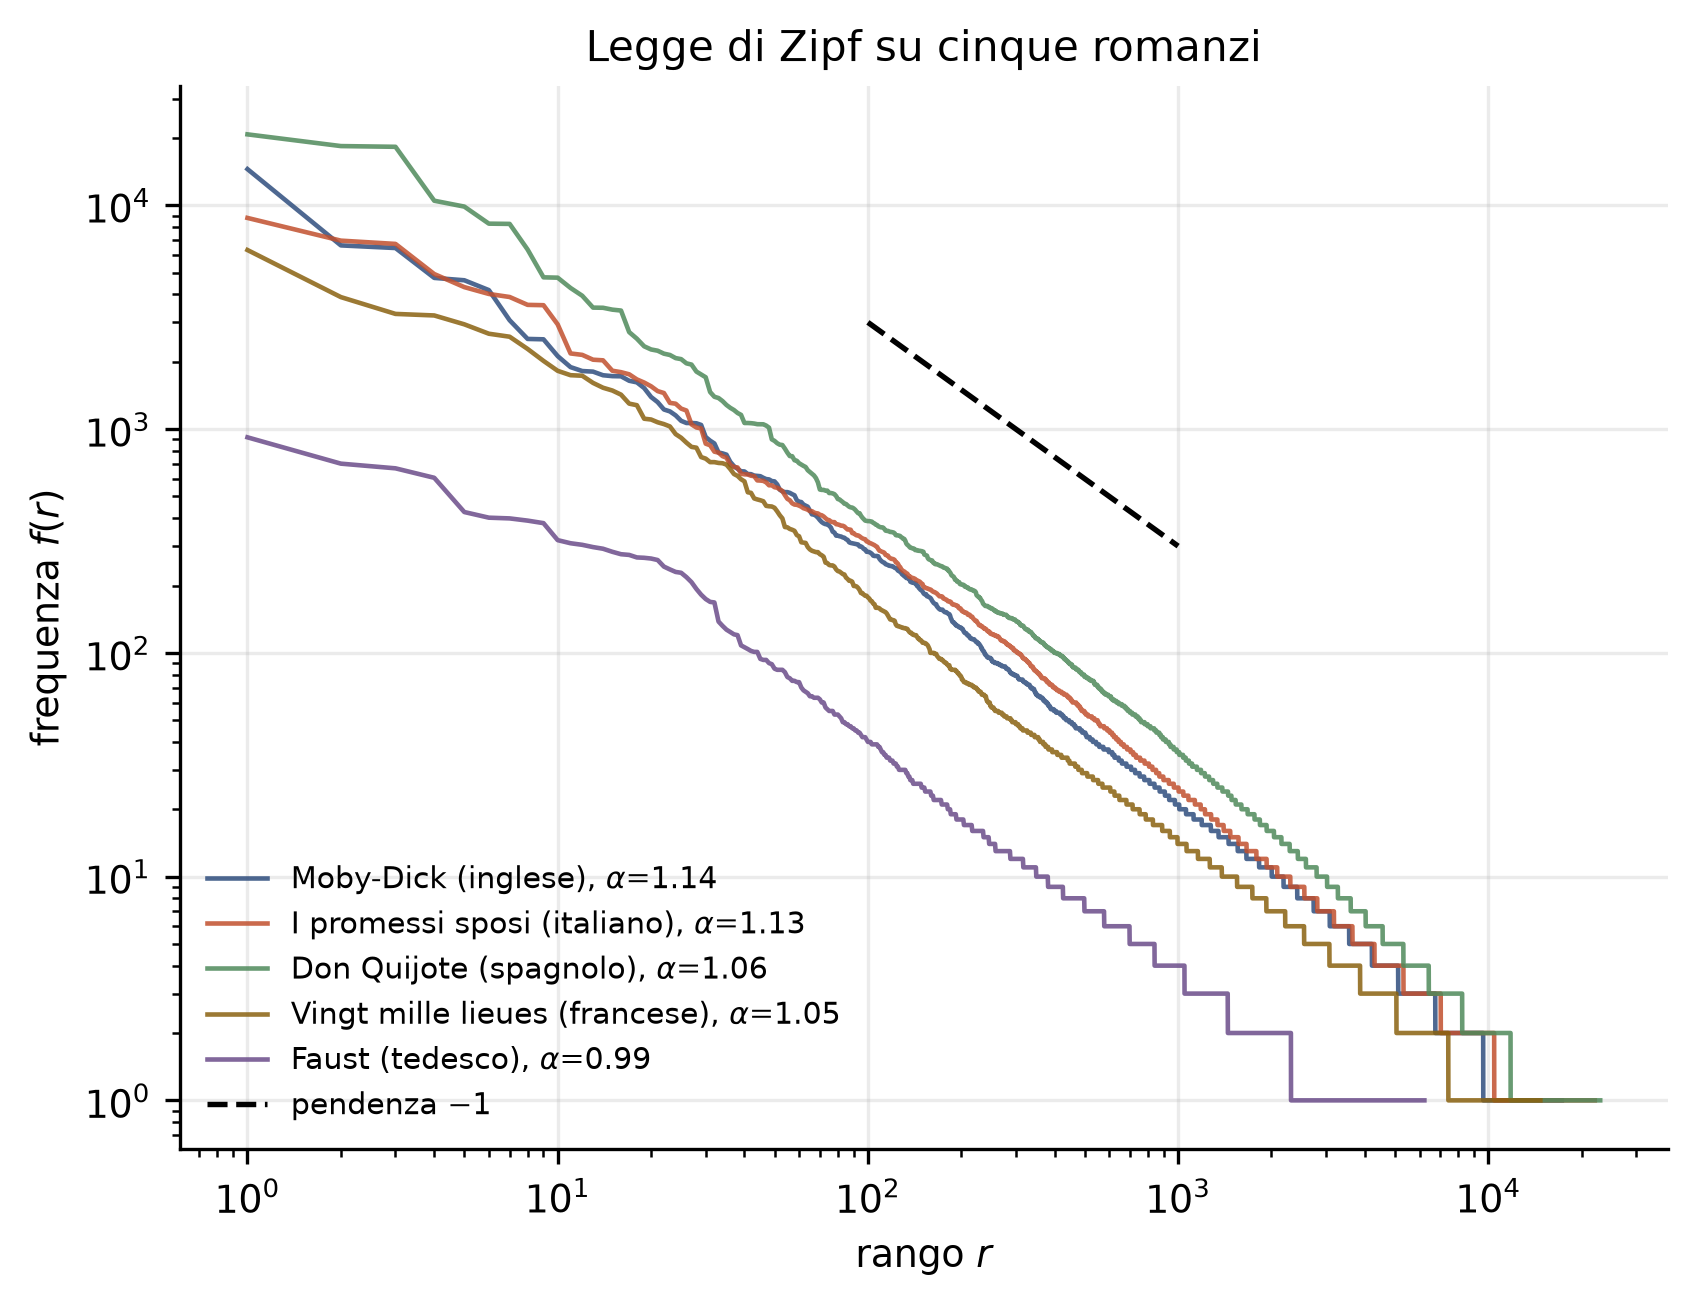
\includegraphics[width=0.82\textwidth]{figure/cap2_zipf_lingue.png}
  \caption{Relazione rango-frequenza per cinque romanzi in altrettante lingue,
  in coordinate bilogaritmiche. Gli esponenti riportati in legenda sono stimati
  per regressione ai minimi quadrati nella finestra di ranghi
  $10^2 \le r \le 10^3$, la stessa impiegata in~\cite{lippi2019}. La retta
  tratteggiata ha pendenza $-1$ ed è riportata come riferimento visivo.}
  \label{fig:zipf}
\end{figure}

Il parametro $\alpha$ risulta positivo e prossimo a 1 nella grande maggioranza
delle lingue esaminate, comprese quelle estinte e quelle costruite
artificialmente. Valori di
$\alpha$ più alti sono sintomo di un vocabolario più povero, poiché un numero
minore di parole esaurisce la maggior parte del testo; valori più bassi
segnalano al contrario una presenza più marcata di parole rare.

I valori misurati sulle cinque opere della Figura~\ref{fig:zipf} sono raccolti
nella Tabella~\ref{tab:zipf-misure}, accanto ai valori medi per lingua riportati
in~\cite{mikhaylovskiy2025zipf} su un corpus di sei opere letterarie in cinque
lingue.

\begin{table}[htbp]
\centering
\small
\begin{tabular}{@{}llrrr@{}}
\toprule
Opera & Lingua & Parole & $|\mathcal{D}|$ & $\alpha$ \\
\midrule
Moby-Dick               & inglese   & \num{219081} & \num{17258} & 1.14 \\
I promessi sposi        & italiano  & \num{239353} & \num{22040} & 1.13 \\
Don Quijote             & spagnolo  & \num{383633} & \num{22943} & 1.06 \\
Vingt mille lieues sous les mers & francese & \num{148923} & \num{14716} & 1.05 \\
Faust                   & tedesco   & \num{30959}  & \num{6221}  & 0.99 \\
\bottomrule
\end{tabular}
\caption{Esponente di Zipf misurato sulle cinque opere della
Figura~\ref{fig:zipf}, con il numero di occorrenze e la dimensione del
dizionario. La stima è condotta sui ranghi $10^2$--$10^3$.}
\label{tab:zipf-misure}
\end{table}

\begin{table}[htbp]
\centering
\small
\begin{tabular}{@{}lcccc@{}}
\toprule
& \multicolumn{2}{c}{$\alpha$ (Zipf)} & \multicolumn{2}{c}{$\gamma_H$ (Heaps)} \\
\cmidrule(lr){2-3}\cmidrule(lr){4-5}
Lingua & parole & token & parole & token \\
\midrule
inglese  & $0.952 \pm 0.072$ & $0.985 \pm 0.054$ & $0.809 \pm 0.027$ & $0.802 \pm 0.024$ \\
tedesco  & $0.959 \pm 0.054$ & $1.024 \pm 0.042$ & $0.846 \pm 0.031$ & $0.793 \pm 0.028$ \\
russo    & $1.043 \pm 0.077$ & $1.009 \pm 0.067$ & $0.916 \pm 0.049$ & $0.805 \pm 0.025$ \\
spagnolo & $0.962 \pm 0.030$ & $1.016 \pm 0.035$ & $0.842 \pm 0.025$ & $0.798 \pm 0.028$ \\
francese & $0.963 \pm 0.033$ & $0.989 \pm 0.042$ & $0.843 \pm 0.020$ & $0.801 \pm 0.018$ \\
\bottomrule
\end{tabular}
\caption{Esponenti medi per lingua riportati in~\cite{mikhaylovskiy2025zipf},
misurati su sei opere letterarie per ciascuna lingua, a livello di parola e di
token. In quel lavoro $\alpha$ è stimato sulla rappresentazione
cumulata della distribuzione anziché sulla relazione rango-frequenza; i due
stimatori coincidono soltanto nel limite $\alpha \to 1$, e i valori non vanno
quindi confrontati direttamente con quelli della
Tabella~\ref{tab:zipf-misure}.}
\label{tab:zipf-letteratura}
\end{table}

Sui testi reali si osservano deviazioni sistematiche dalla~\eqref{eq:zipf}. Su
corpora molto ampi l'esponente resta prossimo a 1 soltanto per le prime migliaia
di parole, mentre la coda continua a seguire una legge di potenza ma con
esponente maggiore~\cite{piantadosi2014}. Le parole più frequenti, inoltre,
mostrano frequenze leggermente inferiori a quelle previste: una deviazione che
Mandelbrot~\cite{mandelbrot1953} corregge introducendo un termine additivo nel
rango,
\begin{equation}
  f(r) \;\propto\; (r + c)^{-\alpha},
  \label{eq:mandelbrot}
\end{equation}
dove la costante $c > 0$ attenua la divergenza della legge di potenza ai ranghi
più bassi, spostando di fatto l'origine dell'asse dei ranghi e rendendo il fit
aderente anche nella regione delle parole più comuni.

\paragraph{Bontà del fit.}
Come si vedrà nei capitoli sperimentali, sui testi generati automaticamente
l'aderenza alla legge di potenza non è garantita. Il solo esponente non è
sufficiente a stabilirla, perché descrive la pendenza media della curva e non la
sua forma: una curva marcatamente incurvata in coordinate bilogaritmiche può
avere la stessa pendenza media di una retta, e restituire quindi un valore di
$\alpha$ del tutto ordinario pur non essendo una legge di potenza. Occorre
perciò una seconda quantità, che misuri quanto i dati si discostino dalla retta
interpolante.

Seguendo~\cite{mikhaylovskiy2025zipf}, la qualità del fit viene stimata con
l'errore percentuale assoluto medio
\begin{equation}
  \mathrm{MAPE} \;=\; \frac{1}{n}\sum_{i=1}^{n}
  \left| \frac{y_i - \hat{y}_i}{y_i} \right|,
  \label{eq:mape}
\end{equation}
dove $n$ è il numero di punti su cui è condotta la regressione, $y_i$ il valore
osservato e $\hat{y}_i$ quello previsto dalla retta interpolante in
corrispondenza dello stesso rango. Il MAPE è nullo per dati perfettamente
allineati e cresce al crescere della distanza relativa dalla retta;
essendo definito su scarti relativi, non dipende dall'unità di misura né
dall'ampiezza delle frequenze, e resta quindi confrontabile fra testi di
lunghezza diversa.

Sul corpus di testi letterari usato in~\cite{mikhaylovskiy2025zipf} il MAPE vale
in media $0.156$ con deviazione standard $0.077$. Nei capitoli sperimentali il
suo minimo in funzione della temperatura di generazione individuerà il regime in
cui il testo prodotto è più vicino a una legge di potenza.

% ---------------------------------------------------------------------
\subsection{Legge di Heaps}
\label{sec:heaps}

Studiando l'andamento di $|\mathcal{D}(t)|$ nei testi letterari emerge una
seconda regolarità, nota come legge di Heaps o, dal nome di chi la formulò per
primo~\cite{herdan1964}, di Herdan--Heaps:
\begin{equation}
  |\mathcal{D}(t)| \;\propto\; t^{\gamma_H}, \qquad \gamma_H \in [0,1] .
  \label{eq:heaps}
\end{equation}
Qui $t$ è la posizione nel testo, misurata in numero di parole,
$|\mathcal{D}(t)|$ la dimensione del dizionario parziale e $\gamma_H$
l'esponente di Heaps. I due estremi dell'intervallo corrispondono a due
comportamenti limite: $\gamma_H = 0$ descrive un dizionario che cessa di
crescere, cioè un testo che non introduce più parole nuove, mentre
$\gamma_H = 1$ descrive un dizionario che cresce proporzionalmente alla
lunghezza, cioè un testo in cui ogni parola è nuova. Poiché il dizionario non
può crescere più rapidamente del testo che lo contiene, si ha necessariamente
$|\mathcal{D}(t)| \le t$, e l'esponente non può eccedere l'unità.

La legge di Heaps quantifica dunque la capacità di un testo di rinnovare il
proprio vocabolario, ed è per questo particolarmente istruttiva se si torna alla
Tabella~\ref{tab:tre-regimi} del Capitolo~\ref{cap:introduzione}. Il primo
esempio, monotono e ripetitivo, cessa rapidamente di accrescere il dizionario;
l'ultimo, in cui i caratteri sono estratti a caso, produce quasi soltanto parole
nuove e fa crescere il dizionario senza saturare. La Figura~\ref{fig:heaps}
mostra le curve dei due casi limite accanto a quelle di tre testi letterari.

\begin{figure}[htbp]
  \centering
  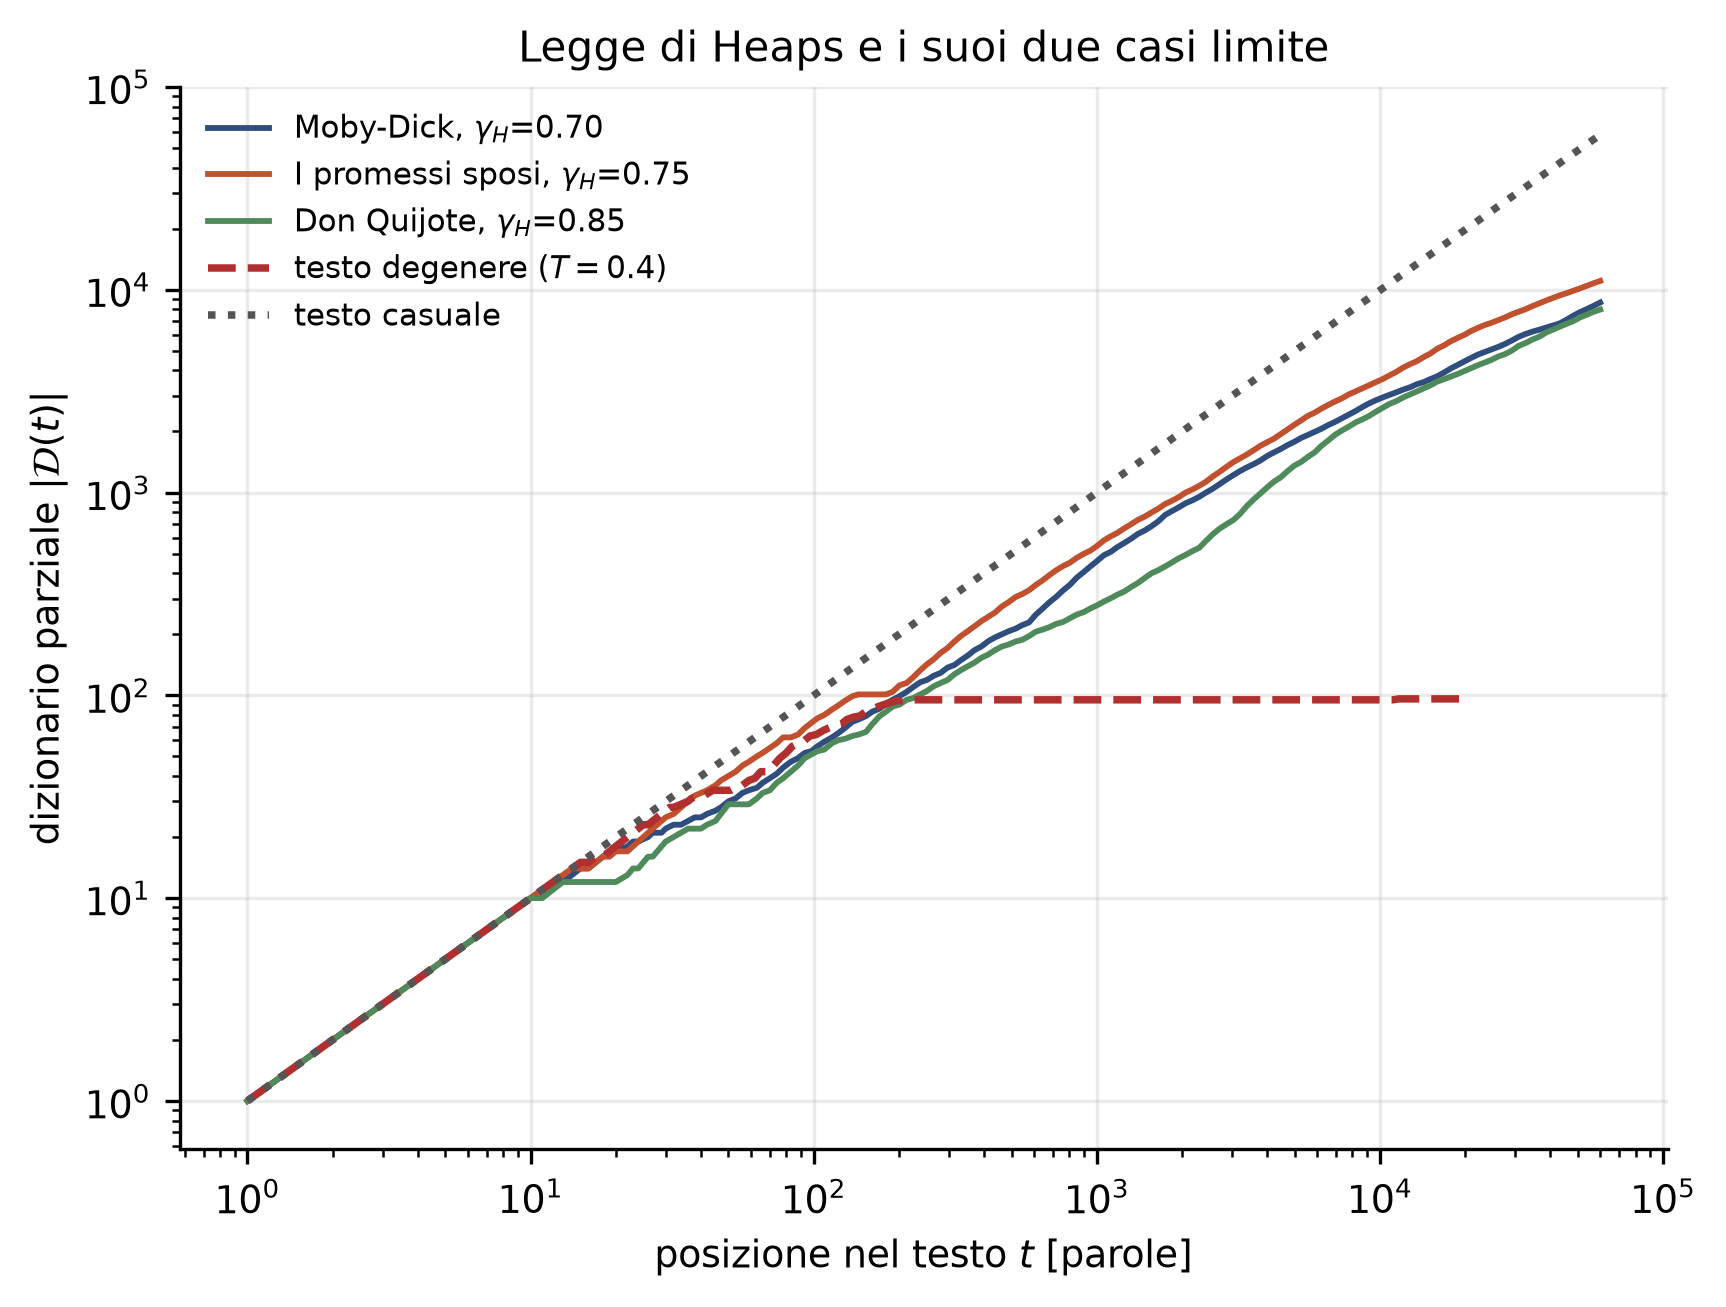
\includegraphics[width=0.82\textwidth]{figure/cap2_heaps_confronto.png}
  \caption{Crescita del dizionario parziale in coordinate bilogaritmiche. Le tre
  curve continue sono testi letterari, con esponente stimato nella regione
  $t > 1000$. La curva tratteggiata è il campione generato a $T = 0.4$ già
  riportato nella Tabella~\ref{tab:tre-regimi}: dopo circa un centinaio di
  parole entra in un ciclo di ripetizione e il dizionario si arresta. La curva
  punteggiata è una sequenza di caratteri casuali, in cui ogni parola è nuova e
  la crescita è esattamente lineare.}
  \label{fig:heaps}
\end{figure}

L'esponente stimato dipende inoltre dall'intervallo su cui viene condotta la
regressione, e quindi dalla lunghezza del testo analizzato. La
Figura~\ref{fig:heaps-finito} mostra l'effetto su tre opere: ripetendo la stima
su prefissi via via più lunghi della stessa opera, $\gamma_H$ decresce in modo
sistematico, di oltre un decimo fra $10^4$ e $10^5$ parole. Il fenomeno è la
prima manifestazione degli effetti di dimensione finita discussi in modo
generale nel §\ref{sec:lunghezza}, ed è già segnalato
in~\cite{mikhaylovskiy2025zipf}, dove si osserva che per $\alpha$ prossimo a 1
la crescita del dizionario è descritta meglio dalla forma $t/\ln t$ che da una
pura legge di potenza. Ai valori di $N$ più bassi la regressione si appoggia a
un intervallo troppo corto e può restituire stime superiori a 1, incompatibili
con il limite teorico: è un artefatto della finestra di fit, non una proprietà
del testo.

\begin{figure}[htbp]
  \centering
  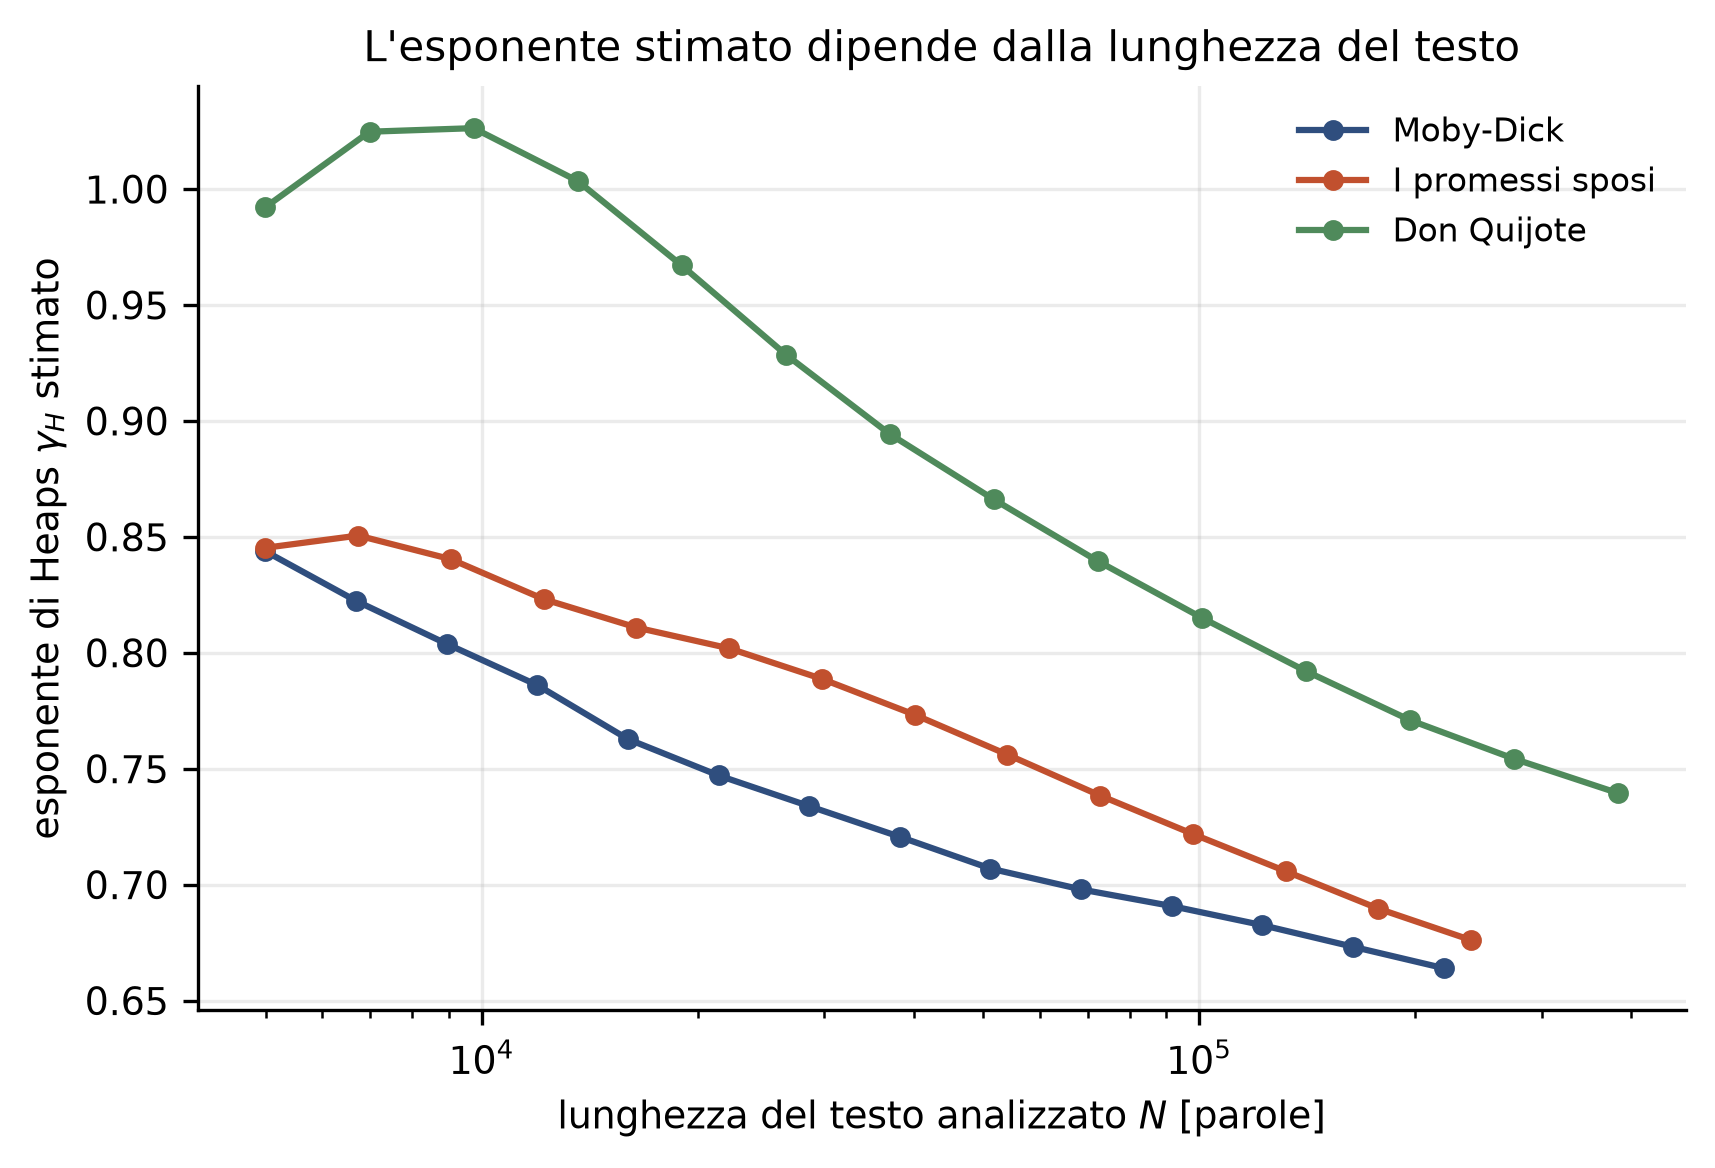
\includegraphics[width=0.78\textwidth]{figure/cap2_heaps_dimensione_finita.png}
  \caption{Esponente di Heaps stimato su prefissi di lunghezza crescente, per tre
  opere in tre lingue diverse, con regressione condotta nella regione $t > 1000$.
  La deriva è sistematica e comune a tutte e tre, ed è quindi una proprietà dello
  stimatore e non di una particolare opera: confrontare esponenti misurati su
  testi di lunghezza diversa non è lecito. Il §\ref{sec:scelte} riprende
  l'effetto su una sola opera, misurandone però l'entità su tutti gli stimatori
  impiegati in questa tesi.}
  \label{fig:heaps-finito}
\end{figure}

\paragraph{Il descrittore $R$.}
Sui testi generati automaticamente la difficoltà è più radicale. A bassa
temperatura di generazione il modello entra in un ciclo di ripetizione e cessa
di produrre parole nuove: la curva $|\mathcal{D}(t)|$ diventa piatta e
la~\eqref{eq:heaps} perde significato. Ad alta temperatura si verifica il caso
opposto, con quasi ogni parola nuova e curva prossima alla linearità. In
entrambe le situazioni la stima di $\gamma_H$ restituisce un numero privo di
contenuto, come mostrano le due curve estreme della Figura~\ref{fig:heaps}.

Per questa ragione in~\cite{mikhaylovskiy2025zipf} viene introdotto un
descrittore che resta definito in ogni regime. Detti $\mathcal{D}_1$ il
dizionario della prima metà del testo e $\mathcal{D}_2$ quello della seconda, si
pone
\begin{equation}
  R \;=\; \frac{|\mathcal{D}_2 \setminus \mathcal{D}_1|}{|\mathcal{D}_1|},
  \label{eq:R}
\end{equation}
cioè il rapporto fra il numero di parole che compaiono per la prima volta nella
seconda metà del testo e il numero di quelle che compaiono per la prima volta
nella prima. Un testo degenerato ha $R$ prossimo a zero, poiché la seconda metà
non introduce nulla di nuovo; un testo in cui ogni parola è nuova ha $R$
prossimo a uno. Sul corpus di opere letterarie intere usato
in~\cite{mikhaylovskiy2025zipf} il valore medio è $R = 0.17$ con deviazione
standard $0.05$.


% ---------------------------------------------------------------------
\section{Correlazioni a lungo raggio}
\label{sec:lrc}

Sia la legge di Zipf sia quella di Heaps ignorano l'ordine dei simboli. Per la
prima l'affermazione è immediata: la~\eqref{eq:zipf} dipende soltanto dai
conteggi delle parole, e un rimescolamento del testo li lascia invariati. Per la
seconda l'invarianza è meno diretta: rimescolando il testo la curva
$|\mathcal{D}(t)|$ cambia realizzazione, perché cambia l'ordine in cui le
parole compaiono per la prima volta, ma il suo andamento medio resta lo stesso, e con esso l'esponente
$\gamma_H$. Entrambe sono quindi proprietà del vocabolario, non della sequenza.

Per misurare le proprietà che dipendono dall'ordine occorre estrarre dal testo
un segnale, cioè una successione finita di valori reali, e studiarne le
correlazioni a scale diverse. La costruzione del segnale non è unica, e ogni
scelta mette in luce aspetti differenti: si può codificare la posizione delle
singole lettere o di classi di lettere, quella delle parole o di classi
grammaticali, oppure la lunghezza delle frasi. In tutti i casi si osserva che il
linguaggio esibisce correlazioni a lungo raggio, con una struttura che si
estende su molti ordini di grandezza~\cite{altmann2012,montemurro2002}.

% ---------------------------------------------------------------------
\subsection{Funzione di autocorrelazione}
\label{sec:acf}

Data una successione $x_1,\dots,x_N$, la funzione di autocorrelazione a distanza
$s$ è
\begin{equation}
  c(s) \;=\; \langle x_n x_{n+s}\rangle
  - \langle x_n\rangle\langle x_{n+s}\rangle ,
  \label{eq:acf}
\end{equation}
dove $\langle\cdot\rangle$ indica la media su tutte le posizioni $n$ compatibili
con la distanza $s$. La forma funzionale di $c(s)$ distingue i regimi di
correlazione.

Se i valori non sono correlati, $c(s)$ è identicamente nulla per $s \neq 0$. Se
$c(s)$ decade esponenzialmente,
$c(s) \sim e^{-s/s_0}$, il segnale si dice correlato a corto raggio: la costante
$s_0$ ha le dimensioni di una distanza e ne fissa la scala caratteristica, nel
senso che oltre poche volte $s_0$ la correlazione è numericamente
indistinguibile da zero. Esiste dunque una distanza tipica oltre la quale due
porzioni di segnale sono indipendenti, e il sistema non possiede struttura al di
là di essa.

Si dice invece che il segnale è correlato a lungo raggio quando il decadimento
segue la legge di potenza
\begin{equation}
  c(s) \;\sim\; s^{-\theta},
  \label{eq:acf-power}
\end{equation}
con $0<\theta<1$. In questo caso non esiste alcuna scala privilegiata: la
funzione~\eqref{eq:acf-power} è invariante di scala, cioè riscalare $s$ di un
fattore costante riscala $c$ di un fattore costante senza modificarne la forma,
e un certo grado di correlazione persiste a tutte le distanze.\footnote{L'esponente
qui indicato con $\theta$ è denotato con $\beta$ in~\cite{altmann2012} e con
$\gamma$ in altra parte della letteratura. Il simbolo è stato cambiato per
evitare la collisione con l'esponente di Heaps e con quello introdotto
nella~\eqref{eq:sigma}.}

La stima diretta di $\theta$ dalla~\eqref{eq:acf-power} è però problematica. Il
segnale è affetto da rumore e, soprattutto, da tendenze di origine esterna che
non sono oggetto di interesse: se la media $\langle x_n\rangle$ differisce fra
la prima e la seconda metà del segnale, come accade proprio quando le
correlazioni sono forti, la~\eqref{eq:acf} risulta distorta. L'esponente va
quindi stimato per via indiretta, e le due sottosezioni seguenti presentano i
due metodi impiegati in questa tesi.

% ---------------------------------------------------------------------
\subsection{Indicatore integrato}
\label{sec:integrato}

Il primo metodo è quello adottato da Altmann, Cristadoro e Degli
Esposti~\cite{altmann2012}, e si applica a segnali binari. Sia dato un testo
come successione simbolica $s = (s_1,\dots,s_N)$. Si definisce una condizione
locale $\mathcal{A}$ che genera la successione binaria
\begin{equation}
  x_k \;=\;
  \begin{cases}
    1 & \text{se $\mathcal{A}$ è soddisfatta in posizione $k$},\\
    0 & \text{altrimenti}.
  \end{cases}
  \label{eq:osservabile}
\end{equation}
L'osservabile può essere la presenza di una data lettera, di una data parola,
oppure l'appartenenza a una classe: per esempio se la lettera in posizione $k$ è
una vocale. L'unità di misura della distanza è il numero di simboli del livello
considerato, ed è questa scelta a rendere confrontabili fra loro una successione
di lettere e una di parole.

Posto
\begin{equation}
  X(t) \;=\; \sum_{j \le t} x_j ,
  \label{eq:conteggio}
\end{equation}
cioè il numero di occorrenze osservate nelle prime $t$ posizioni, si studia la
crescita della varianza del conteggio
\begin{equation}
  \sigma_X^2(t) \;=\; \langle X(t)^2\rangle - \langle X(t)\rangle^2
  \;\simeq\; t^{\gamma}, \qquad \gamma = 2 - \theta .
  \label{eq:sigma}
\end{equation}
La quantità $\sigma_X^2$ è, per costruzione, una somma delle correlazioni a
tutte le distanze inferiori a $t$, e come tale è numericamente assai più stabile
della~\eqref{eq:acf} stimata punto per punto.

Il discrimine fra correlazioni a corto e a lungo raggio non è l'ampiezza di
$c(s)$, ma la sua sommabilità. La~\eqref{eq:conteggio} è formalmente il
cammino percorso da un camminatore che a ogni passo avanza di $x_j$: se i passi
sono indipendenti, o abbastanza rapidamente decorrelati perché $\sum_s c(s)$
converga, vale il teorema del limite centrale e la varianza del cammino cresce
proporzionalmente al numero di passi. Si ha allora diffusione normale,
$\gamma = 1$, esattamente come per il moto browniano. Se invece la somma
diverge, cioè se $\theta \le 1$, i passi restano correlati a ogni scala, il
camminatore tende a proseguire nella direzione già intrapresa e si allontana
dall'origine più rapidamente: la diffusione è anomala e $1 < \gamma < 2$. Il
valore $\gamma = 1$ costituisce dunque il riferimento nullo di tutte le misure
di questo tipo.

La stima di $\gamma$ risente di effetti di tempo finito che la fanno
sottostimare~\cite{altmann2012}: tutti i valori riportati nei capitoli
sperimentali vanno letti come limiti inferiori.

% ---------------------------------------------------------------------
\subsection{Detrended fluctuation analysis}
\label{sec:dfa}

Il secondo metodo è la \emph{detrended fluctuation analysis}, introdotta da
Peng et al.~\cite{peng1994} e applicata ai testi generati automaticamente
in~\cite{lippi2019}. Rispetto all'indicatore integrato presenta il vantaggio
di rimuovere le tendenze locali, e risulta quindi applicabile anche a segnali
non stazionari, cioè segnali le cui proprietà statistiche, tipicamente la
media $\langle x_n \rangle$ o la varianza, non sono costanti lungo la
successione ma derivano lentamente da un estremo all'altro.

La distinzione fra tendenza e correlazione è essenziale, e non riguarda solo
l'origine delle due. Una tendenza è una deriva sistematica e regolare del valore
medio, sovrapposta al segnale da una causa esterna al sistema; una correlazione
è invece una proprietà statistica interna, che lega fra loro le fluttuazioni
attorno a quel valore medio. Il problema pratico è che entrambe producono lo
stesso effetto sulla~\eqref{eq:acf}, gonfiandola a grandi distanze, ed è quindi
necessario eliminare le prime per misurare le seconde. Si potrebbe pensare
sufficiente sottrarre una media mobile di ampiezza fissata, ma in questo modo si
introdurrebbe artificialmente nei dati proprio quella ampiezza come scala
caratteristica, distruggendo le altre.

Il segnale viene costruito codificando ogni carattere del testo con il proprio
rango di frequenza: al carattere più frequente si associa 1, al secondo 2, e
così via. Seguendo~\cite{lippi2019} la codifica avviene a livello di carattere e
conserva punteggiatura, cifre, maiuscole e lettere accentate. Ottenuta la
successione $x_i$ con $i = 1,\dots,N$, la procedura si articola in quattro
passi, qui presentati nella formulazione di~\cite{kantelhardt2001}.

\begin{enumerate}
  \item Si determina il profilo
    \begin{equation}
      Y(i) \;=\; \sum_{k=1}^{i}\bigl(x_k - \langle x\rangle\bigr),
      \label{eq:dfa-profilo}
    \end{equation}
    cioè lo scarto cumulato dalla media. La sottrazione della media non è
    strettamente necessaria, poiché verrebbe comunque eliminata dal detrending.
  \item Si divide il profilo in $N_s = \lfloor N/s \rfloor$ segmenti disgiunti
    di lunghezza $s$.
  \item In ciascun segmento si interpola ai minimi quadrati la tendenza locale,
    ottenendo il polinomio $Y_s(i)$ che approssima il profilo entro quel
    segmento. L'ordine del polinomio determina l'ordine delle tendenze rimosse:
    una DFA di ordine $n$ elimina le tendenze polinomiali fino al grado $n$. In
    questa tesi si impiega l'ordine 1, che rimuove le tendenze lineari locali;
    la robustezza dei risultati rispetto a questa scelta è verificata nel
    §\ref{sec:robustezza}.
  \item Si calcola lo scarto quadratico medio del profilo dalla propria
    tendenza locale, mediando su tutti i segmenti, e si ottiene la funzione di
    fluttuazione
    \begin{equation}
      F(s) \;=\; \left(\frac{1}{N}\sum_{i=1}^{N}
      \bigl(Y(i) - Y_s(i)\bigr)^2\right)^{1/2}.
      \label{eq:dfa-F}
    \end{equation}
\end{enumerate}

La fluttuazione cresce con la lunghezza dei segmenti $s$ e, per un segnale
correlato a lungo raggio, segue la legge di potenza
\begin{equation}
  F(s) \;\sim\; s^{\alpha_{\mathrm{DFA}}} .
  \label{eq:dfa-alpha}
\end{equation}
Per un segnale scorrelato, o correlato a corto raggio, si ha
$\alpha_{\mathrm{DFA}} = 1/2$. Valori superiori indicano correlazioni
persistenti: una fluttuazione positiva tende a essere seguita da un'altra
fluttuazione positiva, e il segnale conserva memoria della propria direzione.
Valori inferiori indicano correlazioni antipersistenti, in cui una fluttuazione
positiva tende a essere seguita da una negativa e il segnale tende a tornare
sui propri passi. Un cammino aleatorio dà $\alpha_{\mathrm{DFA}} = 3/2$: i suoi
incrementi sono scorrelati, ma la successione che ne risulta accumula ogni
deviazione senza riassorbirla, e le fluttuazioni crescono di conseguenza molto
più in fretta. Sul testo letterario di riferimento~\cite{lippi2019} riporta
$\alpha_{\mathrm{DFA}} \simeq 0.65$, contro $0.50$ misurato sulla sua versione
rimescolata: nettamente sopra il riferimento scorrelato e nettamente sotto
quello del cammino aleatorio.

% ---------------------------------------------------------------------
\subsection{Relazione fra i due metodi}
\label{sec:ponte}

I due metodi introdotti misurano la stessa proprietà, e i rispettivi esponenti
sono legati da una relazione semplice. Applicata alla medesima successione,
la~\eqref{eq:dfa-F} coincide, a meno del detrending, con la deviazione standard
del profilo alla scala $s$, cioè $F(s) \simeq \sigma_X(s)$. Elevando al quadrato
e usando la~\eqref{eq:sigma} si ottiene $F(s)^2 \simeq s^{\gamma}$, da cui
\begin{equation}
  \alpha_{\mathrm{DFA}} \;=\; \frac{\gamma}{2} \;=\; 1 - \frac{\theta}{2} .
  \label{eq:ponte}
\end{equation}
La stessa relazione, ricavata per altra via, è riportata
in~\cite{kantelhardt2001}. Nella~\eqref{eq:ponte} $\gamma$ è l'esponente di
crescita della varianza del conteggio definito nella~\eqref{eq:sigma}, mentre
$\theta$ è l'esponente di decadimento dell'autocorrelazione definito
nella~\eqref{eq:acf-power}; i tre esponenti sono dunque tre modi equivalenti di
esprimere la stessa proprietà del segnale.

La~\eqref{eq:ponte} costituisce il ponte fra le due parti sperimentali della
tesi: la diffusione normale $\gamma = 1$, riferimento nullo dell'analisi di
burstiness, corrisponde esattamente al valore $\alpha_{\mathrm{DFA}} = 1/2$,
riferimento nullo dell'analisi sui testi generati. Le due misure non coincidono
esattamente sui dati, poiché la detrended fluctuation analysis rimuove le
tendenze locali mentre l'indicatore integrato no; la differenza fra i due
risultati è informativa proprio quando il segnale non è stazionario.

Un caso limite si presenta con frequenza nei testi generati a bassa
temperatura. Se il testo degenera in un ciclo di ripetizione,
la successione $x_i$ diventa quasi periodica e il profilo~\eqref{eq:dfa-profilo}
oscilla invece di allontanarsi dall'origine: la fluttuazione satura oltre la
lunghezza del periodo e $\alpha_{\mathrm{DFA}}$ scende verso zero. Un esponente
molto basso non segnala quindi assenza di struttura, ma struttura periodica, e
va interpretato congiuntamente a un indicatore diretto di ripetizione.


% ---------------------------------------------------------------------
\section{Burstiness e statistica degli intervalli}
\label{sec:burst}

Le sezioni precedenti permettono di stabilire se un testo possieda correlazioni
a lungo raggio. Questa sezione introduce gli strumenti necessari a stabilire
l'origine di tali correlazioni, che è la domanda posta in~\cite{altmann2012} e
ripresa nella seconda parte sperimentale.

Il punto di partenza è un'osservazione elementare sulla distribuzione delle
parole lungo il testo. Non tutte le parole si distribuiscono allo stesso modo:
alcune ricorrono in modo pressoché uniforme dall'inizio alla fine, altre si
addensano nelle sezioni che trattano l'argomento cui appartengono e sono quasi
assenti altrove. La Figura~\ref{fig:barcode} rende visibile la differenza. Ogni
barra verticale segna una posizione in cui la parola compare; nel primo pannello
la parola è un articolo, nel secondo il nome di un personaggio.

\begin{figure}[htbp]
  \centering
  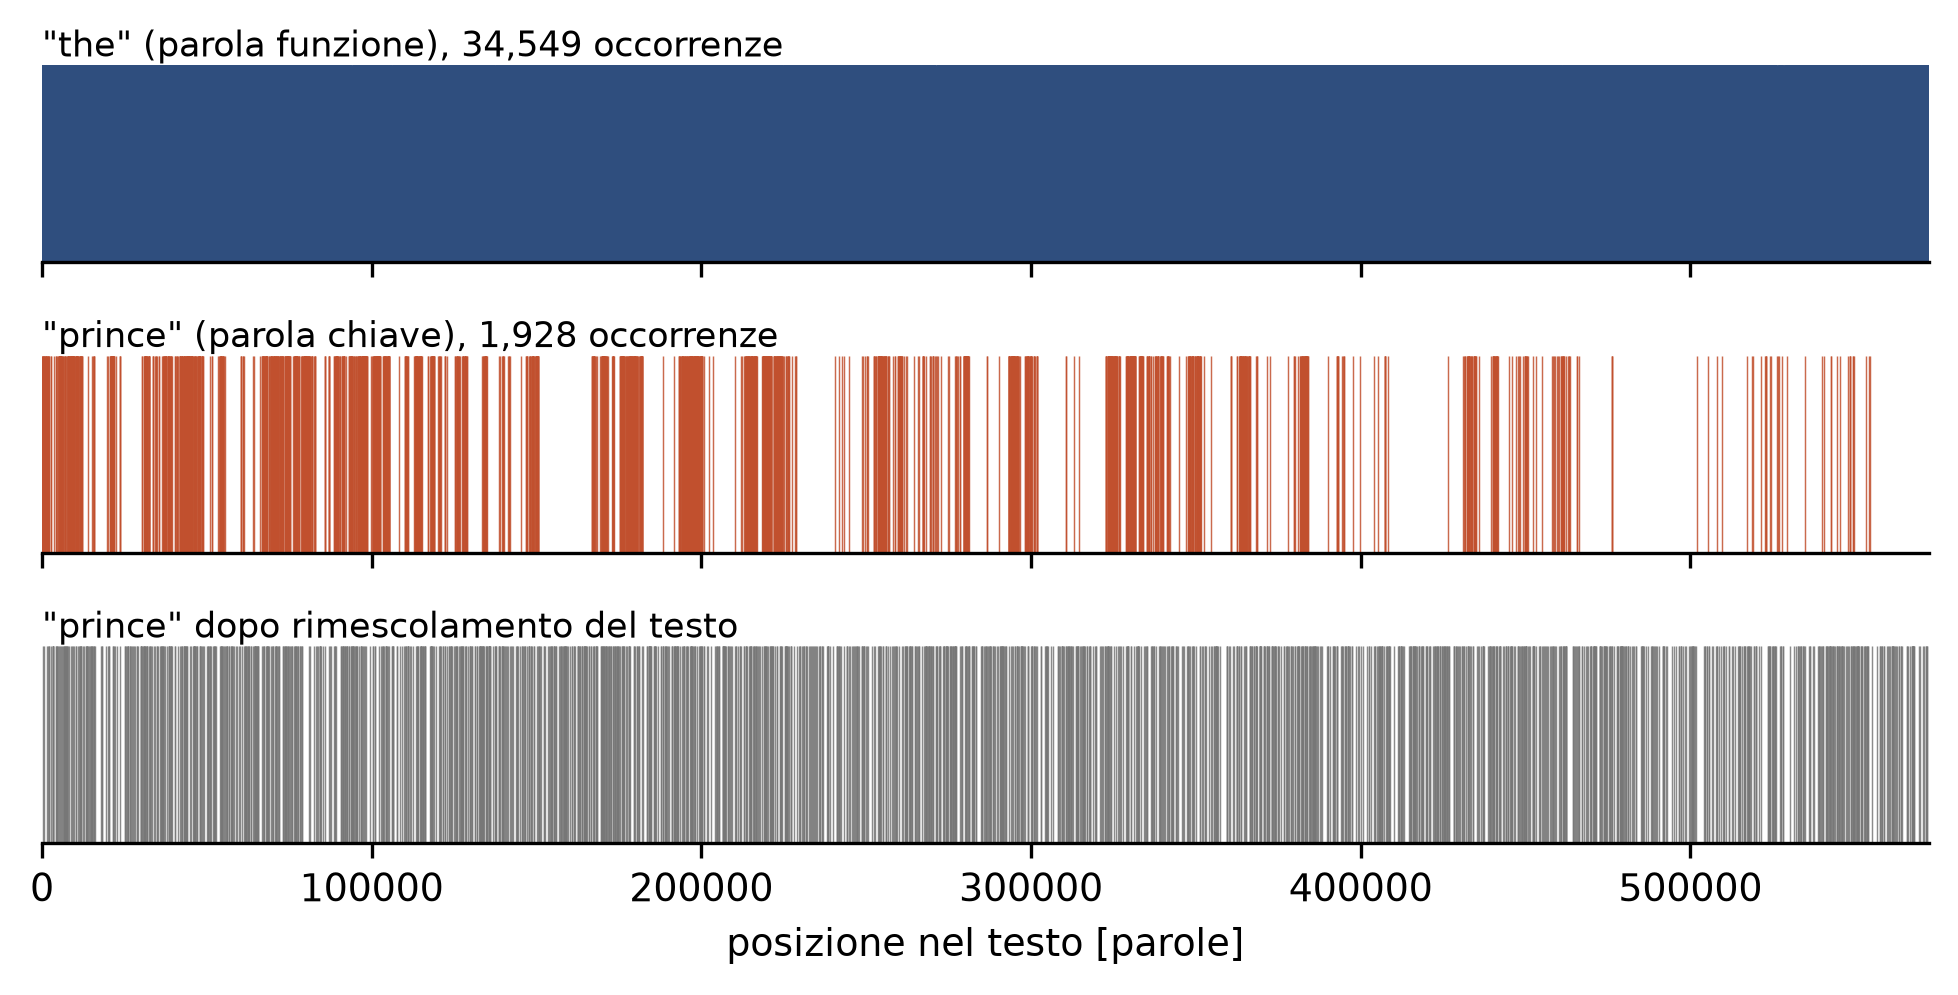
\includegraphics[width=\textwidth]{figure/cap2_burstiness_barcode.png}
  \caption{Posizioni di occorrenza di due parole in \emph{Guerra e pace}. La
  parola funzione \emph{the} riempie il testo in modo uniforme e il pannello
  appare come una banda piena. La parola chiave \emph{prince} si addensa invece
  in gruppi separati da lunghi vuoti, che corrispondono alle porzioni di romanzo
  in cui il personaggio non compare. Il terzo pannello riporta le occorrenze di
  \emph{prince} dopo aver rimescolato le parole del testo: i conteggi sono
  identici, ma i gruppi scompaiono. La struttura visibile nel secondo pannello
  è dunque una proprietà dell'ordine, non delle frequenze.}
  \label{fig:barcode}
\end{figure}

Il fenomeno illustrato dal secondo pannello prende il nome di
\emph{burstiness}: le occorrenze non sono sparse indipendentemente, ma
raggruppate in raffiche separate da intervalli lunghi. Il terzo pannello mostra
perché si tratti di una proprietà dell'ordine e non del vocabolario: il
rimescolamento conserva esattamente il numero di occorrenze, e con esso la legge
di Zipf, ma distrugge la struttura.

Per quantificare il fenomeno si torna alla successione binaria definita
nella~\eqref{eq:osservabile} e si considerano gli intervalli
$\tau_1, \tau_2, \dots$ fra occorrenze consecutive, cioè le distanze in numero
di simboli fra un $1$ e il successivo. La loro distribuzione di probabilità
viene indicata con $p(\tau)$ ed è l'oggetto centrale di questa sezione: tutta
l'informazione sull'ordine che il conteggio delle occorrenze non cattura è
contenuta in $p(\tau)$ e nelle correlazioni fra intervalli successivi.

Il termine di paragone naturale è il processo di Poisson, cioè il processo in
cui ogni posizione ha la stessa probabilità di ospitare un'occorrenza,
indipendentemente da tutte le altre. È il modello del «nessuna struttura»: se le
occorrenze di \emph{prince} fossero poissoniane, il secondo pannello della
Figura~\ref{fig:barcode} sarebbe indistinguibile dal terzo. Per un processo di
Poisson gli intervalli sono distribuiti esponenzialmente e indipendenti fra
loro, e si dimostra che la loro deviazione standard eguaglia la media,
$\sigma_\tau = \langle\tau\rangle$.

Si misura quindi la burstiness con il coefficiente di variazione
\begin{equation}
  \mathrm{cv} \;=\; \frac{\sigma_\tau}{\langle\tau\rangle},
  \label{eq:cv}
\end{equation}
pari a 1 nel caso poissoniano, maggiore di 1 quando le occorrenze si addensano
in raffiche separate da vuoti lunghi e minore di 1 quando sono distribuite in
modo più regolare di quanto il caso comporti. Una misura equivalente, ma
limitata all'intervallo $[-1,1]$ e quindi più comoda per il confronto fra
sequenze diverse, è l'indice proposto da Goh e Barabási~\cite{goh2008},
\begin{equation}
  B \;=\; \frac{\sigma_\tau - \langle\tau\rangle}
                {\sigma_\tau + \langle\tau\rangle} .
  \label{eq:goh}
\end{equation}

% ---------------------------------------------------------------------
\subsection{Le due origini delle correlazioni}
\label{sec:origini}

Il contributo centrale di~\cite{altmann2012} consiste nell'osservare che una
varianza del conteggio che cresce più che linearmente può avere due origini
distinte. Il legame è fornito dallo spettro di potenza a frequenza nulla.

Lo spettro di potenza $S(\omega)$ di una successione descrive come la sua
varianza si distribuisce fra le diverse frequenze $\omega$, ed è la trasformata
di Fourier della funzione di autocorrelazione. Il valore a frequenza nulla,
$S(0)$, raccoglie il contributo delle fluttuazioni più lente, quelle su scale
comparabili con la lunghezza dell'intera successione: è quindi la quantità che
diverge esattamente quando esistono correlazioni a lungo raggio, e che resta
finita quando le correlazioni sono sommabili. Per una successione di occorrenze
descritta dagli intervalli $\tau_i$ vale
\begin{equation}
  S(0) \;=\; \frac{\sigma_\tau^2}{\langle\tau\rangle^3}
  \left(1 + 2\sum_{k\ge1} c_\tau(k)\right),
  \label{eq:eq4}
\end{equation}
dove $c_\tau(k)$ è l'autocorrelazione della successione degli intervalli, cioè
la correlazione fra $\tau_i$ e $\tau_{i+k}$.

La~\eqref{eq:eq4} è il perno dell'intera analisi, perché mostra che $S(0)$ può
divergere in due modi indipendenti. Il primo è la divergenza di $\sigma_\tau$,
cioè una coda pesante di $p(\tau)$: il testo contiene vuoti così lunghi che la
varianza degli intervalli non converge. Il secondo è la non sommabilità di
$c_\tau(k)$, cioè il fatto che gli intervalli siano essi stessi correlati fra
loro. Nella formula resta implicito che cosa questo comporti: $c_\tau(k) > 0$
significa che a un intervallo più lungo della media tende a seguirne un altro
più lungo della media, e quindi che i vuoti si
raggruppano fra loro invece di alternarsi ai riempimenti. Anche con una
$p(\tau)$ a varianza finita, un simile raggruppamento produce fluttuazioni
lente del conteggio e fa divergere la somma.

I due meccanismi sono distinti, perché l'uno riguarda quanto sono lunghi i
vuoti e l'altro come sono disposti, e la~\eqref{eq:eq4} da sola non li separa.

Nei testi reali, di lunghezza finita e con la coda tagliata
(§\ref{sec:coda}), nessuna delle due quantità diverge davvero: ciò che si
misura sono i loro analoghi a finestra finita, e i due null model del
§\ref{sec:null} servono appunto a separarli senza dover decidere quale delle
due divergenze sarebbe realizzata nel limite.

% ---------------------------------------------------------------------
\subsection{I null model A1 e A2}
\label{sec:null}

La separazione si ottiene con due rimescolamenti controllati, costruiti in modo
da distruggere selettivamente uno solo dei due meccanismi.

Il primo, indicato con A1, permuta gli zeri e gli uni della successione binaria.
Conserva soltanto il numero di occorrenze e distrugge tanto la coda di $p(\tau)$
quanto $c_\tau(k)$: è il rimescolamento già illustrato nel terzo pannello della
Figura~\ref{fig:barcode}. Ha funzione di controllo, poiché il risultato è noto a
priori: deve restituire un esponente $\hat\gamma_{A1}$ prossimo a 1, e un valore
diverso segnala un difetto della procedura di misura prima ancora che una
proprietà dei dati.

Il secondo, indicato con A2, permuta fra loro gli intervalli $\tau_i$ senza
alterarne l'insieme. Conserva quindi esattamente $p(\tau)$, e con essa
$\sigma_\tau$, ma distrugge ogni correlazione fra intervalli successivi.
L'esponente risultante $\hat\gamma_{A2}$ isola dunque il solo contributo della
burstiness.

Poiché A2 rimuove un contributo che è di norma non negativo, ci si attende la
disuguaglianza
\begin{equation}
  \hat\gamma \;\ge\; \hat\gamma_{A2},
  \label{eq:disug1}
\end{equation}
che in~\cite{altmann2012} è riportata come regolarità empirica, non come
conseguenza necessaria, e che il §\ref{sec:coda-risultati} verifica
direttamente su tutti i corpora. Fornisce quindi un ulteriore controllo interno
alla misura. Risulta naturale
definire la quota di burstiness
\begin{equation}
  q \;=\; \frac{\hat\gamma_{A2} - 1}{\hat\gamma - 1},
  \label{eq:quota}
\end{equation}
prossima a 1 quando la correlazione proviene interamente dalla coda di $p(\tau)$
e prossima a 0 quando proviene interamente da $c_\tau(k)$: $q$ misura cioè quale
frazione dell'eccesso di correlazione sia attribuibile alla sola burstiness.

Il denominatore della~\eqref{eq:quota} è però piccolo nei corpora poco
correlati, dove $\hat\gamma$ è di poco superiore a 1, e $q$ risulta di
conseguenza uno stimatore rumoroso. Per questa ragione, in questo lavoro $q$
viene calcolata separatamente per ciascun documento e riassunta con mediana e
quartili anziché come rapporto fra medie: si tratta di una scelta metodologica
adottata qui, non di una prescrizione della letteratura, motivata dal fatto che
il rapporto fra due medie non coincide con la media dei rapporti quando il
denominatore ha varianza comparabile al proprio valore.

% ---------------------------------------------------------------------
\subsection{Coda della distribuzione degli intervalli}
\label{sec:coda}

Il legame quantitativo fra burstiness ed esponente di correlazione richiede una
forma esplicita per $p(\tau)$. Assumendo una legge di potenza pura e intervalli
scorrelati si ottiene
\begin{equation}
  p(\tau) \sim \tau^{-\mu}, \quad c_\tau(k) = \delta(k), \quad 2 < \mu < 3
  \;\Longrightarrow\;
  \gamma = 4 - \mu .
  \label{eq:eq8}
\end{equation}
La condizione $2<\mu<3$ individua il regime in cui la media di $\tau$ esiste ma
la varianza diverge, ed è esattamente il regime in cui la~\eqref{eq:cv} non
converge al crescere della lunghezza del testo.

La legge di potenza pura è però un modello idealizzato, e lo stesso
\cite{altmann2012} lo riconosce nel formulare la~\eqref{eq:eq8}. Scendendo
nella gerarchia linguistica i vuoti lunghi vengono spezzati: una lettera che
compone una parola chiave compare anche in tutte le altre parole del testo, e i
lunghi intervalli in cui la parola chiave è assente si riempiono di occorrenze
dovute ad altre parole. Esiste quindi una lunghezza $\tau_c$ oltre la quale gli
intervalli, semplicemente, non si osservano più: è il cut-off che quel lavoro
introduce con questo stesso argomento, senza però stimarlo. Il modello
realistico è la legge di potenza troncata
\begin{equation}
  p(\tau) \;\sim\; \tau^{-\mu}\,e^{-\tau/\tau_c},
  \label{eq:troncata}
\end{equation}
che ha due vantaggi rispetto alla forma pura. Il primo è descrittivo: separa due
proprietà distinte della coda, la pendenza $\mu$ nella regione intermedia e la
distanza $\tau_c$ alla quale la coda viene tagliata, mentre un fit con la sola
legge di potenza le confonde in un unico esponente apparente. Il secondo è che
rende la distribuzione normalizzabile e a varianza finita per ogni $\mu$,
eliminando la necessità di assumere $2<\mu<3$. In presenza di cut-off la
burstiness contribuisce solo per distanze inferiori a $\tau_c$, e
la~\eqref{eq:eq8} non vale più come uguaglianza ma come disuguaglianza,
\[
  \hat\gamma_{A2} \;\le\; 4 - \mu ,
\]
che vincola dall'alto l'esponente misurato sul null model A2.

Nella~\eqref{eq:troncata} $\mu$ e $\tau_c$ agiscono sulla forma della coda in
modo parzialmente sovrapposto: rendere la coda più ripida aumentando $\mu$
produce quasi lo stesso effetto che tagliarla prima riducendo $\tau_c$. Di
conseguenza esistono molte coppie $(\mu, \tau_c)$ diverse fra loro che
descrivono i dati quasi altrettanto bene, cioè che rendono quasi identica la
verosimiglianza, la probabilità di osservare i dati raccolti sotto quei valori
dei parametri. La conseguenza pratica è duplice: gli intervalli di confidenza
vanno calcolati per profilo, esplorando cioè la verosimiglianza al variare di
un parametro con l'altro riottimizzato, e non con la formula asintotica che
presuppone parametri indipendenti; e $\mu$ non va riportato separatamente dal
$\tau_c$ che lo accompagna, perché da solo non identifica la coda.

% ---------------------------------------------------------------------
\subsection{Effetti di dimensione finita}
\label{sec:lunghezza}

Per la legge di potenza pura, quando $\mu<3$ la varianza di $p(\tau)$ diverge e
la stima di $\sigma_\tau$ non converge. Con il taglio della~\eqref{eq:troncata}
i momenti sono invece finiti, ma $\tau_c$ è esso stesso una grandezza che
dipende dalla finestra, e la conseguenza osservabile è la medesima:
la~\eqref{eq:cv} cresce monotonamente con la finestra di osservazione,
poiché finestre più lunghe campionano vuoti più lunghi. Lo stesso vale, in
misura diversa, per l'esponente di Heaps e per il MAPE, come già mostrato nella
Figura~\ref{fig:heaps-finito} del §\ref{sec:heaps}.

La deriva non è un difetto di stima che una procedura migliore potrebbe
eliminare: è una proprietà delle quantità stesse, che su una finestra finita non
hanno un valore limite. Ne discendono vincoli su come i confronti possono essere
condotti, ed è il Capitolo~\ref{cap:metodi} a fissarli, insieme alla misura
dell'entità dell'effetto sui corpora effettivamente impiegati.


% ---------------------------------------------------------------------
\subsection{Entropia degli intervalli}
\label{sec:entropia-intervalli-def}

Il coefficiente di variazione della~\eqref{eq:cv} ha due limiti che il
§\ref{sec:lunghezza} rende evidenti. Il primo è la dipendenza dalla lunghezza
di analisi, che ne impedisce il confronto fra corpora misurati su finestre
diverse. Il secondo è più sottile: $\mathrm{cv}$ è un rapporto e quindi non
cambia se tutti gli intervalli vengono moltiplicati per una costante, ma nei
confronti fra corpora la dilatazione non è uniforme. Quando il tempo si conta in
caratteri, un corpus con frasi mediamente più lunghe produce intervalli più
lunghi ai soli livelli definiti su unità linguistiche, e non a quello dei
caratteri: la scala dei $\tau$ non è la stessa nei due corpora e ogni
differenza ne risente.

Serve quindi una misura di irregolarità che dipenda dalla forma della
distribuzione degli intervalli e non dalla loro scala. Si adotta a questo
scopo l'entropia differenziale del logaritmo degli intervalli, stimata per
spaziature d'ordine con lo stimatore di Vasicek~\cite{vasicek1976}, diminuita
di quella che si otterrebbe da un processo di Poisson con lo stesso numero di
eventi e la stessa media: \begin{equation} J \;=\; h(\ln\tau) \;-\;
h_{\mathrm{Poisson}}(n, \langle\tau\rangle). \label{eq:entropia-intervalli}
\end{equation}

Le due operazioni rispondono ai due limiti. Prendere il logaritmo rende $J$
invariante per dilatazione: moltiplicare tutti i $\tau$ per una costante trasla
$\ln\tau$ senza modificarne l'entropia differenziale, cosicché la diversa
lunghezza delle frasi non produce alcun effetto. Sottrarre il valore poissoniano
fissa lo zero sul processo privo di struttura, come per la~\eqref{eq:cv}, ma con
un vantaggio ulteriore: il termine sottratto viene simulato con lo stesso
stimatore e con gli stessi $n$ e $\langle\tau\rangle$ del dato osservato, per
cui il bias dello stimatore si cancella in larga parte nella differenza invece
di sommarsi.

\paragraph{Fin dove l'invarianza tiene.}
L'argomento appena dato riguarda una distribuzione continua. Gli intervalli fra
occorrenze in un testo sono invece numeri interi, e l'arrotondamento agli interi
non commuta con la dilatazione: comprimere una distribuzione fino a intervalli
di poche unità ne cancella la forma, e $J$ ne risente. Il pannello A della
Figura~\ref{fig:invarianza-J} misura l'entità del fenomeno moltiplicando per una
costante gli intervalli generati da una stessa legge. Per
$\langle\tau\rangle \gtrsim 30$ le curve sono piatte entro due centesimi di bit
e l'invarianza tiene; per $\langle\tau\rangle = 5$ una dilatazione di un fattore
cinquanta sposta $J$ di $0.59$ bit. L'invarianza è dunque asintotica nel valore
medio degli intervalli, non esatta.

La distinzione ha una conseguenza pratica sui livelli linguistici. Ai due
livelli lessicali, dove la diversa lunghezza delle frasi si fa sentire,
l'intervallo medio nei corpora del Capitolo~\ref{cap:risultati2} vale fra $340$
e $1900$ caratteri, quindi in pieno regime asintotico. Ai livelli delle lettere e
degli spazi, dove l'intervallo medio scende sotto la decina, i valori di $J$
risentono della quantizzazione e vanno letti come descrittori relativi, validi
per confrontare corpora misurati allo stesso modo e non come distanze assolute
dal processo di Poisson.

Il pannello B della stessa figura verifica la cancellazione del bias facendo
crescere il numero di intervalli da $30$ a $1000$ su cinque leggi di forma nota.
La deriva residua non supera $0.07$ bit su un intervallo in cui $n$ cambia di un
fattore trentatré, ed è massima sulle distribuzioni log-normali. La
cancellazione è quindi buona ma non completa, e differenze di $J$ inferiori a un
decimo di bit fra sequenze di numerosità molto diversa non sono interpretabili.

\begin{figure}[htbp]
  \centering
  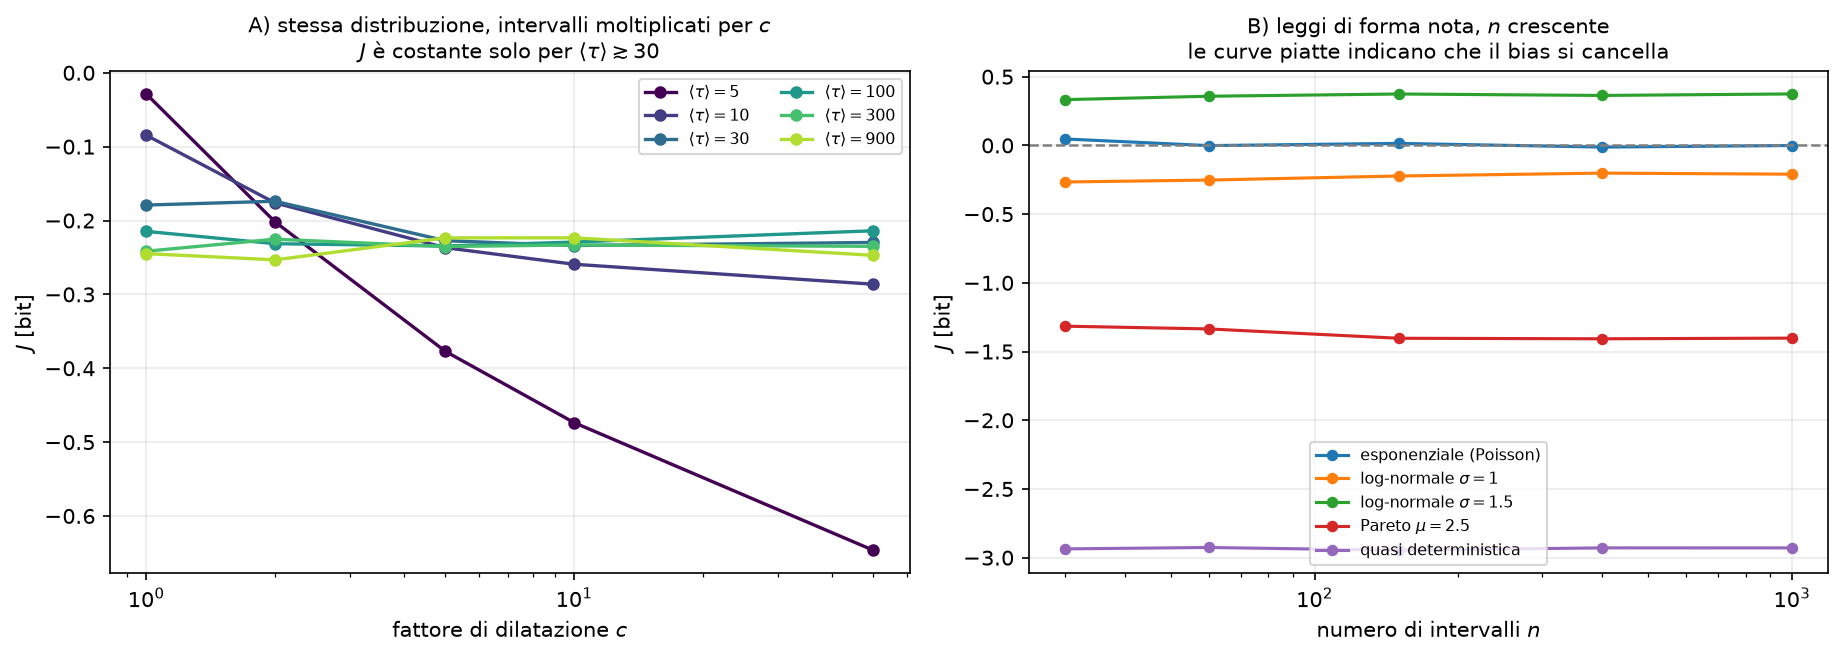
\includegraphics[width=\textwidth]{figure/cap2_invarianza_J.png}
  \caption{Limiti di validità della~\eqref{eq:entropia-intervalli}, misurati
  sullo stimatore effettivamente impiegato. A: intervalli estratti da una stessa
  legge log-normale e moltiplicati per un fattore $c$, per sei valori
  dell'intervallo medio di partenza; una curva piatta indica invarianza. Sotto
  $\langle\tau\rangle \simeq 30$ la quantizzazione agli interi la distrugge. B:
  $J$ su cinque leggi di forma nota al crescere del numero di intervalli; lo
  scostamento fra gli estremi quantifica il bias che la sottrazione del termine
  poissoniano non elimina.}
  \label{fig:invarianza-J}
\end{figure}

Valori positivi di $J$ indicano intervalli distribuiti in modo più irregolare di
un processo di Poisson, valori negativi una regolarità superiore a quella del
caso. La quantità non compare in nessuno dei lavori di riferimento ed è
introdotta qui; il §\ref{sec:entropia-intervalli} ne verifica la stabilità
rispetto alla lunghezza di analisi e la impiega per neutralizzare l'effetto
appena descritto.


% ---------------------------------------------------------------------
\section{Entropia e compressione}
\label{sec:entropia}

Il concetto di disordine di un testo e la nozione di entropia sono già stati
introdotti nel Capitolo~\ref{cap:introduzione}. Trattandosi di un concetto
centrale per questo lavoro, in questa sezione viene definito in modo formale e
ne viene esplicitato il legame con gli algoritmi di compressione, che è lo
strumento con cui l'entropia verrà effettivamente stimata sui testi.

% ---------------------------------------------------------------------
\subsection{Entropia e predicibilità}
\label{sec:entropia-def}

Si consideri una sorgente che emette simboli da un alfabeto finito
$\mathcal{X}$. Per una singola variabile aleatoria $X$ che assume il valore
$x \in \mathcal{X}$ con probabilità $p(x)$, l'entropia di
Shannon~\cite{shannon1948} è
\begin{equation}
  H(X) \;=\; -\sum_{x \in \mathcal{X}} p(x) \log_2 p(x),
  \label{eq:H-singola}
\end{equation}
espressa in bit, e misura l'incertezza media sull'esito dell'estrazione.

I simboli di un testo non sono però indipendenti, e l'entropia di una singola
lettera non descrive la sorgente: sapere che in inglese la lettera più frequente
è \emph{e} dice poco, mentre sapere che dopo \emph{th} segue quasi sempre
\emph{e} dice molto. Occorre quindi considerare blocchi di simboli. Detta
$H(X_1,\dots,X_n)$ l'entropia congiunta di un blocco di lunghezza $n$, definita
dalla~\eqref{eq:H-singola} applicata alla distribuzione congiunta dei blocchi, si
definisce il tasso di entropia della sorgente come
\begin{equation}
  h \;=\; \lim_{n\to\infty} \frac{H(X_1,\dots,X_n)}{n} .
  \label{eq:tasso-entropia}
\end{equation}
Il limite esiste per sorgenti stazionarie ed ergodiche~\cite{cover2006} e
quantifica l'incertezza media per simbolo una volta tenuto conto di tutte le
dipendenze, comprese quelle a lunga distanza. È questa, e non
la~\eqref{eq:H-singola}, la quantità pertinente per un testo.

Il teorema della codifica di sorgente~\cite{cover2006} lega $h$ alla
comprimibilità: il tasso di entropia è un limite inferiore alla lunghezza media
per simbolo di qualunque codifica senza perdita. Stimare l'entropia di un testo
e stimarne la comprimibilità sono quindi, entro le approssimazioni del caso, lo
stesso problema.

Il legame si comprende in modo intuitivo tornando ai casi limite della
Tabella~\ref{tab:tre-regimi}. Un algoritmo di compressione senza perdita opera
sostituendo alle porzioni di testo che si ripetono un riferimento
all'occorrenza precedente, più breve del testo che rimpiazza. Nel testo monotono
il medesimo gruppo di parole ricorre per l'intera lunghezza del documento: dopo
la prima occorrenza tutto il resto è un riferimento, il file compresso è
minuscolo e il tasso di entropia è prossimo a zero, perché il simbolo successivo
è quasi sempre determinato da quelli che lo precedono. Nella sequenza casuale,
al contrario, nessuna porzione si ripete: non esiste nulla cui fare riferimento,
il compressore non guadagna nulla e il tasso di entropia è massimo, perché ogni
simbolo è imprevedibile a partire dai precedenti. Il linguaggio naturale si
colloca fra i due estremi, e la quantità di compressione che ammette è una
misura diretta di quanta struttura possiede.

\paragraph{Stimatori di Lempel--Ziv.}
La stima diretta di $h$ dalla~\eqref{eq:tasso-entropia} per conteggio di blocchi
è impraticabile: il numero di blocchi distinti di lunghezza $n$ cresce
esponenzialmente con $n$, e la dimensione campionaria necessaria a stimarne le
probabilità cresce di conseguenza. Nessun testo reale è abbastanza lungo.

Si ricorre allora agli stimatori della famiglia Lempel--Ziv~\cite{ziv1977},
che aggirano il problema misurando le ripetizioni invece delle probabilità.
L'idea è la seguente: si scorre la successione e, a ogni posizione $i$, si cerca
la più lunga sottostringa che inizi in $i$ e sia già comparsa in precedenza,
detta $\Lambda_i$ la sua lunghezza. In un testo molto ripetitivo i match sono
lunghi, in un testo casuale sono corti. Si dimostra che, per una sorgente
stazionaria ed ergodica, la lunghezza media di tali match cresce come il
logaritmo della finestra esplorata e che
\begin{equation}
  h \;=\; \lim_{n\to\infty}
  \left\langle \frac{\log_2 n}{\Lambda_i} \right\rangle ,
  \label{eq:lz-entropia}
\end{equation}
dove la media è presa sulle posizioni $i$. La~\eqref{eq:lz-entropia} converge
assai più rapidamente del conteggio di blocchi e mantiene buone proprietà anche
in presenza di correlazioni a lungo raggio, che è la ragione per cui viene
adottata qui: le sorgenti considerate in questa tesi hanno, per costruzione,
memoria lunga.

% ---------------------------------------------------------------------
\subsection{Stima della cross-entropia e della divergenza}
\label{sec:crossparsing}

Le quantità introdotte finora descrivono un testo singolo. Per confrontare due
testi occorre la cross-entropia, che misura il costo di codificare un testo
usando la statistica di un altro.

L'algoritmo di cross-parsing di Ziv e Merhav~\cite{ziv1993} estende
la~\eqref{eq:lz-entropia} a due successioni. Data la successione $x$ da
misurare e la successione di riferimento $y$, si scorre $x$ da sinistra a destra
e la si decompone in frasi successive, dove ogni frase è la più lunga
sottostringa che, a partire dalla posizione corrente, compaia da qualche parte
in $y$; raggiunto il punto in cui il match si interrompe, si chiude la frase e
se ne apre una nuova. Il numero di frasi così ottenute viene indicato con
$c(x|y)$ ed è la quantità che misura la somiglianza fra i due testi: se $x$ e
$y$ provengono dalla stessa sorgente, le frasi sono lunghe e poche; se
provengono da sorgenti diverse, i match si interrompono presto e le frasi sono
molte. La stima della cross-entropia è
\begin{equation}
  h(x \,|\, y) \;=\; \frac{c(x|y)\,\log_2 |y|}{|x|},
  \label{eq:crossparsing}
\end{equation}
espressa in bit per simbolo, dove $|x|$ e $|y|$ sono le lunghezze delle due
successioni.

La divergenza di Kullback--Leibler è lo strumento con cui si quantifica quanto
due distribuzioni di probabilità differiscano fra loro. Date due distribuzioni
$P$ e $Q$ sullo stesso alfabeto, essa è definita come
\begin{equation}
  D(P\|Q) \;=\; \sum_{x} P(x) \log_2 \frac{P(x)}{Q(x)}
  \;=\; H_P(Q) - H(P),
  \label{eq:kl-def}
\end{equation}
dove $H_P(Q)$ è la cross-entropia fra le due distribuzioni. La~\eqref{eq:kl-def}
si interpreta come il numero medio di bit sprecati per simbolo codificando una
sorgente $P$ con un codice ottimizzato per $Q$: vale zero se e solo se
$P = Q$ ed è positiva altrimenti.

In termini di successioni, la~\eqref{eq:kl-def} si stima come differenza fra due
cross-entropie: dividendo $x$ in due metà $x_1$ e $x_2$ e prendendo da $y$ un
prefisso $y_1$ della stessa lunghezza di $x_1$, si pone
\begin{equation}
  D(x \,\|\, y) \;=\; h(x_2 \,|\, y_1) \;-\; h(x_2 \,|\, x_1) .
  \label{eq:kl}
\end{equation}
La seconda metà di $x$ viene cioè codificata due volte, una volta usando come
riferimento un testo estraneo e una volta usando la prima metà di $x$ stesso, e
si misura quanto costa in più la prima operazione.

L'appaiamento delle lunghezze dei due riferimenti non è un dettaglio.
La~\eqref{eq:crossparsing} dipende dalla lunghezza del riferimento, poiché un
riferimento più lungo contiene più sottostringhe e produce una cross-entropia
minore a parità di sorgente. Se i due termini della~\eqref{eq:kl} usassero
riferimenti di lunghezza diversa, la differenza conterrebbe un termine spurio
che può superare in modulo il segnale da misurare e produrre stime negative,
impossibili per la~\eqref{eq:kl-def}. Con $|y_1| = |x_1|$ il termine spurio si
cancella, e la costruzione soddisfa la proprietà verificabile $D(x\|x) = 0$
esattamente, impiegata nei capitoli sperimentali come test dello stimatore.

Poiché la~\eqref{eq:kl} non è simmetrica, mentre per confrontare due corpora
serve una quantità che non dipenda da quale dei due venga posto come
riferimento, seguendo~\cite{lippi2019} viene adottata la divergenza
simmetrizzata
\begin{equation}
  D_s(x,y) \;=\; \tfrac{1}{2}\bigl[D(x\|y) + D(y\|x)\bigr].
  \label{eq:kl-sym}
\end{equation}

% ---------------------------------------------------------------------
\subsection{Misure basate su compressione}
\label{sec:compressione}

Le stime della sottosezione precedente usano la compressione come strumento
teorico, attraverso il conteggio delle frasi. Un secondo gruppo di misure,
introdotto in questo contesto da Hadad et al.~\cite{hadad2026}, impiega invece
direttamente un compressore reale come sonda della regolarità strutturale, senza
passare per una stima di entropia.

Detta $C(x)$ la dimensione in byte del testo $x$ dopo la compressione, si
definisce il rapporto di compressione
\begin{equation}
  R_{\mathrm{gzip}}(x) \;=\; \frac{C(x)}{|x|},
  \label{eq:cratio}
\end{equation}
tanto minore quanto più il testo è regolare. Il pedice ricorda l'algoritmo
impiegato e distingue la quantità dal descrittore $R$ della~\eqref{eq:R}.

Da esso derivano la compressione condizionata
$\bigl(C(x+y) - C(x)\bigr)/|y|$, dove $x+y$ indica la concatenazione, che stima
il costo incrementale di codificare la seconda metà di un documento dopo aver
già codificato la prima e misura quindi quanto la seconda metà sia prevedibile
a partire dalla prima; e la distanza normalizzata di compressione~\cite{li2004}
\begin{equation}
  \mathrm{NCD}(x,y) \;=\;
  \frac{C(xy) - \min\{C(x),C(y)\}}{\max\{C(x),C(y)\}} .
  \label{eq:ncd}
\end{equation}
Applicata fra un testo e una sua permutazione, la~\eqref{eq:ncd} misura quanta
parte della comprimibilità dipenda dall'ordine delle parole e non dalla sola
composizione lessicale: è quindi l'analogo, in chiave di compressione, del
confronto fra i pannelli della Figura~\ref{fig:barcode}.


% ---------------------------------------------------------------------
\section{Token ed embedding}
\label{sec:token}

Nel §\ref{sec:scala} si è assunta la parola come unità fondamentale del testo,
in quanto più piccola porzione dotata di significato autonomo per un lettore
umano. Questa scelta non vale più per gli algoritmi di generazione automatica
del testo e, in particolare, per i modelli linguistici di grandi dimensioni.

Si riprenda la frase già usata come esempio,
\emph{Se pensi di comprendere la meccanica quantistica, non comprendi la
meccanica quantistica.} Per un lettore umano essa si scompone come nella
Figura~\ref{fig:scomp-parole}: dodici parole più la punteggiatura, ciascuna
delle quali ha un significato che si può cercare in un dizionario.

\begin{figure}[htbp]
  \centering
  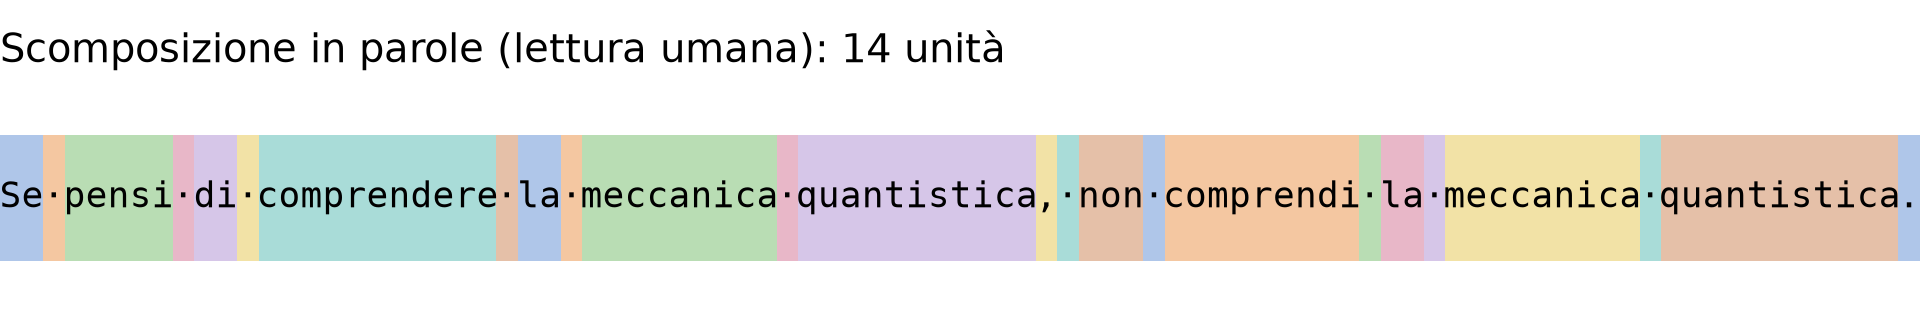
\includegraphics[width=\textwidth]{figure/cap2_scomposizione_parole.png}
  \caption{Scomposizione in parole. Ogni blocco è un'unità dotata di
  significato autonomo; il punto mediano segnala gli spazi.}
  \label{fig:scomp-parole}
\end{figure}

Per un modello linguistico la stessa frase si scompone invece come nella
Figura~\ref{fig:scomp-token}.

\begin{figure}[htbp]
  \centering
  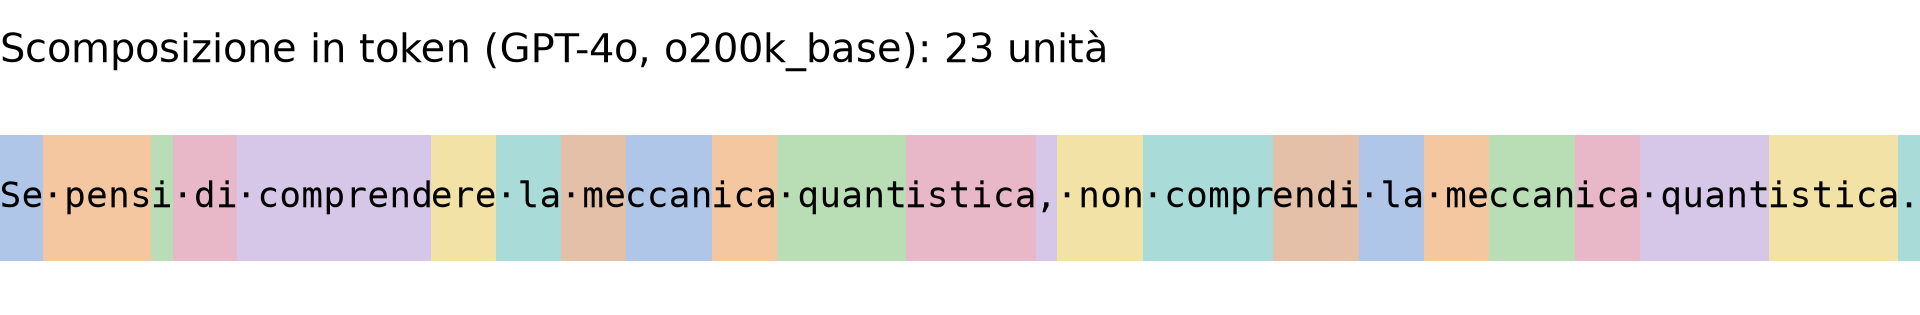
\includegraphics[width=\textwidth]{figure/cap2_scomposizione_token.png}
  \caption{Scomposizione in token della stessa frase, ottenuta con il
  tokenizzatore \texttt{o200k\_base} impiegato da GPT-4o. Le unità sono
  ventitré, non coincidono con le parole e in generale non hanno significato
  autonomo.}
  \label{fig:scomp-token}
\end{figure}

La frase non è divisa né in lettere né in parole, ma in gruppi di lettere
chiamati \emph{token}. Alcuni token coincidono con parole intere
(\texttt{·la}, \texttt{·non}), altri sono frammenti privi di significato
(\texttt{ccan}, \texttt{istica}). Si osservi in particolare la coppia
\emph{comprendere} e \emph{comprendi}: la prima si scompone in
\texttt{·comprend} e \texttt{ere}, la seconda in \texttt{·compr} e
\texttt{endi}. Due forme della stessa radice vengono dunque tagliate in punti
diversi, e il modello non riceve alcuna indicazione esplicita del fatto che
condividano la radice. Lo spazio, inoltre, non separa i token ma vi è
incorporato: la maggior parte dei token inizia con uno spazio, e la
segmentazione del testo in unità precede logicamente qualunque nozione di
parola.

La conversione avviene tramite un algoritmo detto \emph{tokenizzatore}, che
traduce un testo scritto in una qualsiasi lingua e in un qualsiasi alfabeto in
una sequenza di token estratti da un dizionario ampio ma finito, costruito una
volta per tutte a partire da un grande corpus. I dizionari dei tokenizzatori
più diffusi hanno dimensioni dell'ordine di $10^5$ elementi: quello di GPT-4o,
\texttt{o200k\_base}, ne conta \num{200019}; \texttt{cl100k\_base}, impiegato
come unità di analisi nei capitoli sperimentali per le ragioni discusse nel
Capitolo~\ref{cap:metodi}, ne conta \num{100277}; i modelli Qwen2.5 analizzati
in questa tesi ne condividono uno di circa \num{151000} voci. Poiché il
dizionario è finito ma le lingue possibili sono molte, i testi nelle lingue
meno rappresentate nel corpus di costruzione vengono frammentati in un numero
di token assai maggiore rispetto all'inglese.

Proprio come le parole per gli esseri umani, per un modello linguistico sono i
token a trasportare significato. Il significato non è però un'etichetta
associata al token, bensì una posizione: tramite un'operazione detta
\emph{embedding} ogni token viene mappato in un vettore di uno spazio a molte
dimensioni, e la geometria di quello spazio codifica le relazioni fra i token.
Vettori vicini corrispondono a token che compaiono in contesti simili, e
direzioni ricorrenti nello spazio corrispondono a relazioni ricorrenti nel
linguaggio.

La Figura~\ref{fig:embedding} mostra la proprietà su un caso concreto. I vettori
di trenta parole inglesi, appartenenti a cinque famiglie semantiche, sono
proiettati sulle prime due componenti principali dello spazio: le parole di
ciascuna famiglia si dispongono in gruppi distinti, benché la costruzione dei
vettori non abbia mai fatto uso di alcuna classificazione semantica, ma soltanto
delle co-occorrenze osservate in un corpus.

\begin{figure}[htbp]
  \centering
  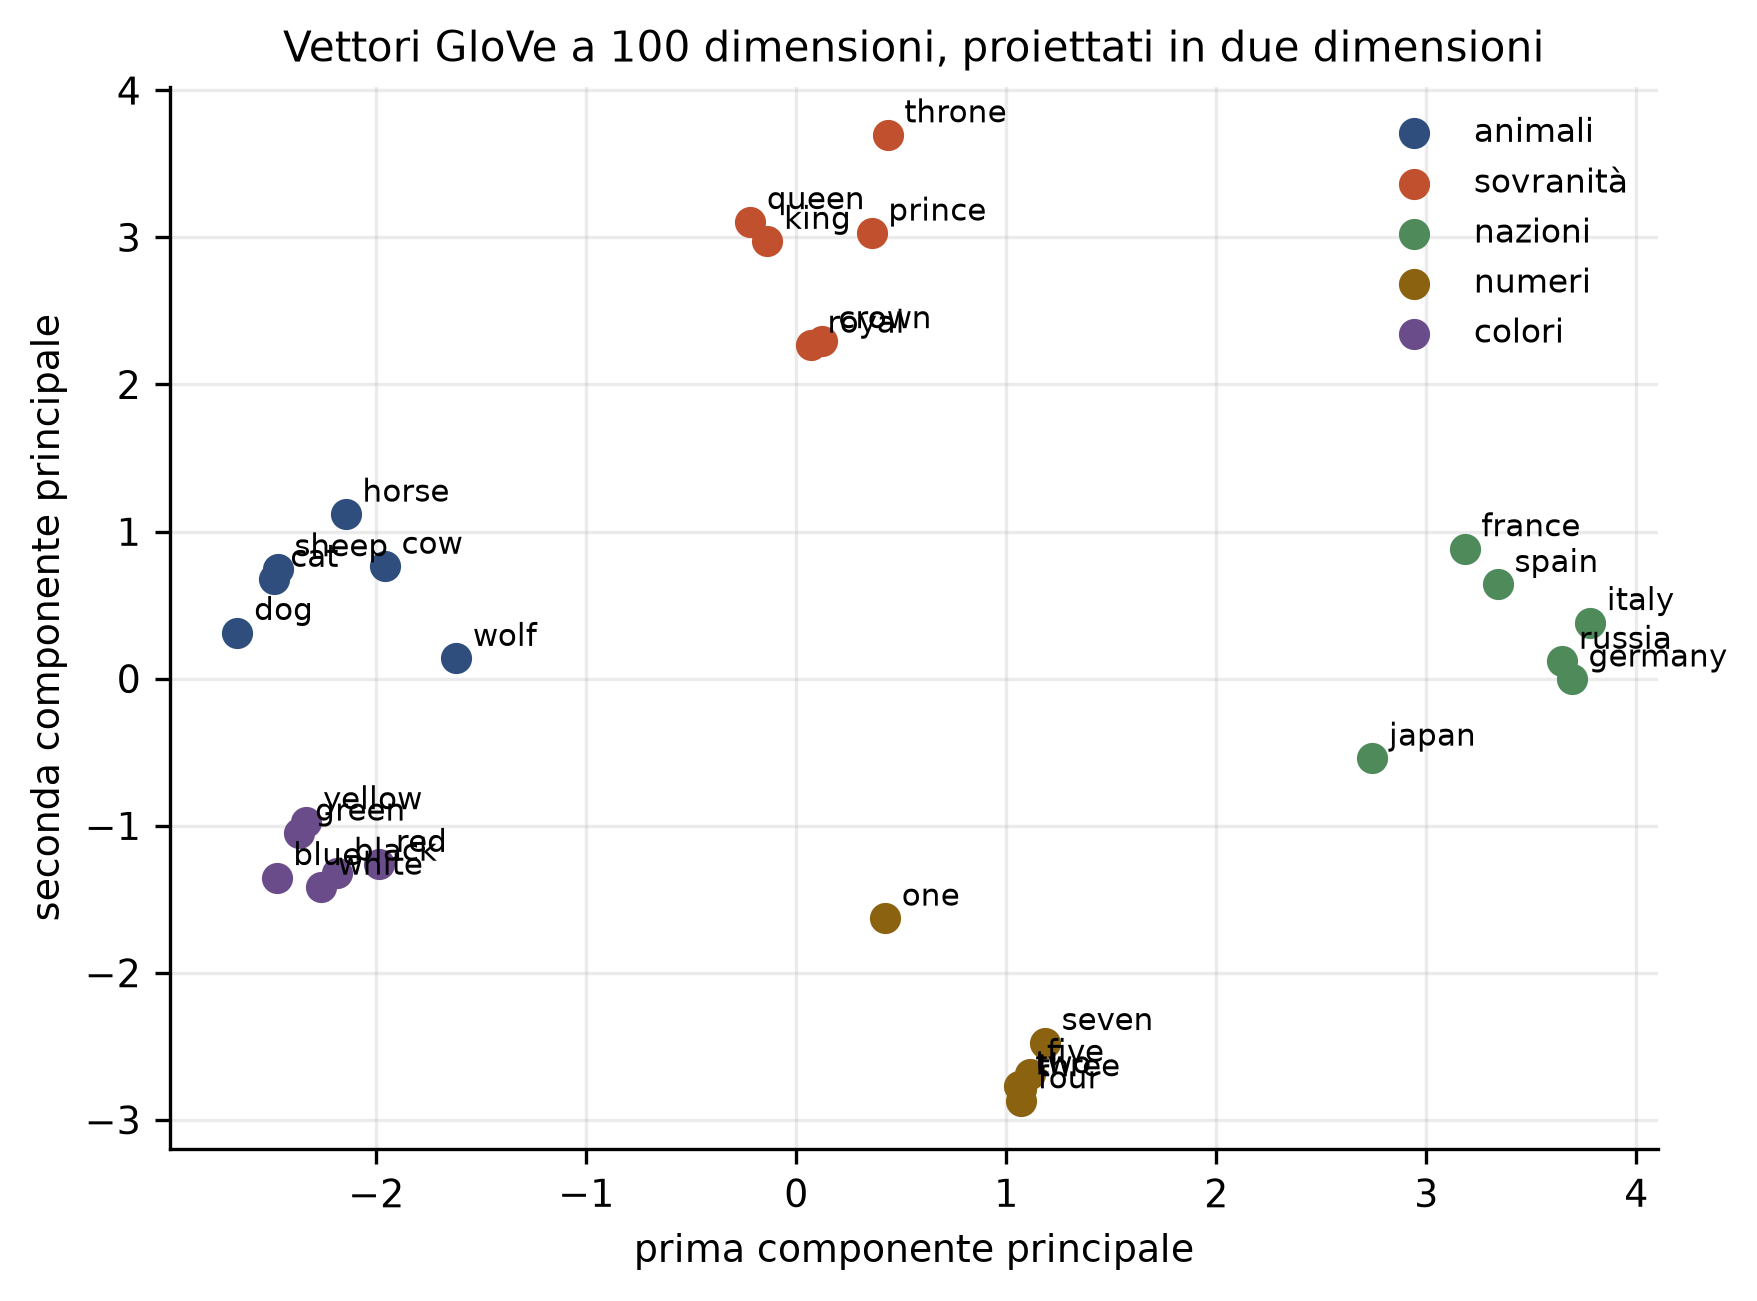
\includegraphics[width=0.82\textwidth]{figure/cap2_embedding_2d.png}
  \caption{Trenta parole inglesi rappresentate dai rispettivi vettori GloVe a
  100 dimensioni, proiettati sulle prime due componenti principali. Le cinque
  famiglie semantiche formano gruppi separati senza che alcuna informazione
  semantica sia stata fornita all'algoritmo. La proiezione conserva soltanto una
  parte della struttura, poiché riduce cento dimensioni a due: la vicinanza
  visibile in figura è una condizione sufficiente, non necessaria, alla
  vicinanza nello spazio originario.}
  \label{fig:embedding}
\end{figure}

I due spazi vettoriali che compaiono in questo lavoro hanno natura diversa. Ogni modello linguistico possiede una propria matrice di embedding,
appresa durante l'addestramento insieme a tutti gli altri parametri, e i cui
vettori non sono direttamente confrontabili fra modelli diversi: fra i modelli
analizzati in questa tesi la dimensione di tale spazio passa da 1536 per il
modello da 1.5 miliardi di parametri a 5120 per quello da 14 miliardi. Gli embedding impiegati nelle analisi di
questa tesi sono invece vettori GloVe a 100 dimensioni, pre-addestrati su un
corpus esterno e identici per tutti i testi esaminati: la scelta è dettata dalla
necessità di misurare i testi generati da modelli diversi con lo stesso metro, e
segue l'impostazione di~\cite{mikhaylovskiy2025states}. Nel
§\ref{sec:traiettoria} tali vettori verranno usati per trasformare un testo in
una traiettoria nello spazio semantico e studiarne l'autocorrelazione.


% ---------------------------------------------------------------------
\section{Generazione autoregressiva e temperatura}
\label{sec:temperatura}

Un modello linguistico autoregressivo, data una sequenza di token $t_{1:m}$,
sceglie il token successivo estraendolo da una distribuzione di probabilità che
dipende dalla sequenza stessa. La probabilità dell'intera sequenza si
decompone per mezzo della regola della catena,
\begin{equation}
  P(t_{1:m}) \;=\; \prod_{k=1}^{m} P(t_k \mid t_{1:k-1}),
  \label{eq:autoregressivo}
\end{equation}
e il modello è addestrato ad approssimare i singoli fattori
$P(t_k \mid t_{1:k-1})$, cioè a prevedere ogni token a partire da tutti quelli
che lo precedono. La generazione consiste nell'applicare ripetutamente questa
previsione, aggiungendo di volta in volta il token estratto alla sequenza che
condiziona l'estrazione successiva.

\paragraph{Origine della distribuzione condizionata.}
Il modo in cui il modello costruisce $P(t_k \mid t_{1:k-1})$ è ciò che
distingue le architetture moderne da quelle precedenti, ed è rilevante per
questo lavoro. I modelli oggi in uso si basano sull'architettura
\emph{transformer}~\cite{vaswani2017}, il cui elemento caratteristico è il
meccanismo di \emph{attenzione}. In esso ogni posizione della sequenza calcola
un peso per ciascuna delle posizioni precedenti e costruisce la propria
rappresentazione come combinazione pesata di quelle: il token in posizione $k$
può quindi attingere direttamente a qualunque token precedente, per lontano che
sia, senza che l'informazione debba propagarsi attraverso le posizioni
intermedie.

È una differenza sostanziale rispetto ai modelli ricorrenti, in cui
l'informazione proveniente da una posizione lontana deve attraversare tutte
quelle interposte e si degrada di conseguenza. Nel transformer il cammino fra
due posizioni qualsiasi ha lunghezza costante, e questo rende l'architettura in
linea di principio capace di rappresentare dipendenze fra porzioni di testo
molto distanti fra loro. È il meccanismo che, negli attuali modelli, potrebbe
dare origine alle correlazioni a lungo raggio descritte nel §\ref{sec:lrc}, e
una delle ragioni per cui ha senso cercarle nel testo generato. La capacità di
rappresentare tali dipendenze non implica però che il modello le riproduca
effettivamente, e l'attenzione opera comunque entro una finestra di contesto
finita: stabilire se le correlazioni siano presenti nel
testo prodotto resta una questione empirica, ed è precisamente quella affrontata
nei capitoli sperimentali.

\paragraph{Temperatura.}
Il modello non produce direttamente probabilità, ma valori reali detti
\emph{logit}, indicati con $u_1,\dots,u_{|\mathcal{L}|}$, uno per ciascun
elemento del dizionario $\mathcal{L}$. Essi vengono convertiti in distribuzione
di probabilità da una funzione softmax riscalata da un parametro
$T$~\cite{ackley1985}:
\begin{equation}
  p(t = \mathcal{L}_l \mid t_{1:i-1}) \;=\;
  \frac{\exp(u_l / T)}{\sum_{l'} \exp(u_{l'} / T)} .
  \label{eq:softmax}
\end{equation}

Il parametro $T$ prende il nome di temperatura, e la denominazione non è una
semplice analogia. Ponendo $E_l = -u_l$, la~\eqref{eq:softmax} coincide con la
distribuzione di Boltzmann $p_l \propto e^{-E_l/T}$ di un sistema a
$|\mathcal{L}|$ stati in equilibrio termico alla temperatura $T$. Questa
identificazione è ciò che giustifica la ricerca, nel testo generato, dei
fenomeni caratteristici dei sistemi termodinamici, e in particolare delle
transizioni di fase discusse nel §\ref{sec:fasi}.

I due limiti sono immediati. Per $T\to0$ la distribuzione si concentra sul token
di logit massimo e la generazione diventa deterministica; per $T\to\infty$ tende
alla distribuzione uniforme sull'intero dizionario, indipendentemente dal
contesto. Fra i due estremi, valori $T<1$ concentrano la massa di probabilità
sugli eventi più probabili, mentre valori $T>1$ la ridistribuiscono verso quelli
meno probabili. La temperatura non modifica dunque ciò che il modello ha
appreso, ma soltanto quanto fedelmente la generazione segue la distribuzione
appresa.

Nella pratica corrente la generazione impiega anche il troncamento della
distribuzione, nelle varianti top-$k$~\cite{fan2018} e
top-$p$~\cite{holtzman2020}, e penalità che scoraggiano la ripetizione. Tutti
questi meccanismi agiscono sulla stessa distribuzione e introducono un secondo
parametro d'ordine, rendendo impossibile attribuire alla sola temperatura il
comportamento osservato. Per questa ragione, e coerentemente con la scelta
esplicita di~\cite{mikhaylovskiy2025zipf}, i dati analizzati in questa tesi sono
stati generati impiegando il solo campionamento per temperatura.


% ---------------------------------------------------------------------
\section{Fasi e stato critico}
\label{sec:fasi}

Una fase di un sistema fisico è uno stato, tipicamente di equilibrio, dotato di
proprietà macroscopiche caratteristiche e stabile in una regione dello spazio
dei parametri; alla frontiera di tali regioni avviene una transizione di fase.
Secondo la classificazione di Ehrenfest~\cite{ehrenfest1933} una transizione di
ordine $n$ è una discontinuità nella derivata $n$-esima dell'energia libera.

Applicare alla lettera questa classificazione al testo generato non è però
possibile. Il sistema considerato non ha un'energia libera di cui prendere
derivate, non è in equilibrio con alcun bagno termico e
non possiede un limite termodinamico, poiché il numero di token di un documento
resta finito. Ciò che rende legittimo il linguaggio delle fasi è la
corrispondenza stabilita nel §\ref{sec:temperatura}: la~\eqref{eq:softmax}
coincide con una distribuzione di Boltzmann in cui i logit giocano il ruolo di
energie e il parametro di campionamento quello di temperatura. La distribuzione
condizionata da cui ogni token viene estratto è dunque, letteralmente, una
distribuzione di Gibbs, e $T$ ne è la temperatura. Quello che resta analogia, e
non identità, è il passaggio dal singolo token al documento: nulla garantisce
che le proprietà collettive di una sequenza generata token per token si
comportino come le proprietà macroscopiche di un sistema all'equilibrio. Il
vocabolario di Ehrenfest viene perciò impiegato in senso descrittivo, per
nominare regioni di comportamento qualitativamente diverso separate da
variazioni rapide, e non per rivendicare una transizione di fase in senso
termodinamico.

Ciò che rende il concetto utile è il comportamento nel punto critico che
separa due fasi: là le correlazioni decadono a legge di potenza e la loro
portata diverge, e molte grandezze osservabili esibiscono lo stesso andamento.
Il criterio inverso, per cui dove compare una legge di potenza si sospetta uno
stato critico, va maneggiato con prudenza, perché distribuzioni a legge di
potenza si generano in molti modi che con la criticità non hanno rapporto, dal
semplice prodotto di variabili aleatorie ai processi di preferential
attachment. Preso da solo, l'andamento a legge di potenza di una quantità non
dimostra nulla. Acquista forza quando più osservabili indipendenti cambiano
regime allo stesso valore del parametro di controllo, ed è in questa forma che
viene impiegato nel §\ref{sec:tstar}: non la legge di potenza di una misura,
ma la convergenza di criteri costruiti per scopi diversi.

Il quadro è stato applicato ai modelli linguistici in~\cite{nakaishi2024}, dove
la temperatura di campionamento separa una fase a bassa temperatura,
caratterizzata da strutture ripetitive, da una ad alta temperatura in cui il
testo è incomprensibile. La tesi sostenuta in quel lavoro è che il linguaggio
naturale si collochi \emph{sul} punto critico fra le due: nello spazio dei
processi stocastici che generano successioni di simboli, il processo
corrispondente a una lingua naturale giacerebbe sulla superficie critica che
separa le due regioni, e un modello addestrato su quella lingua definisce una
famiglia di processi che quella superficie attraversa al variare di $T$. Il
risultato è verificato su modelli da 160 milioni a 2.8 miliardi di parametri, su
sei lingue e su due diverse mappature del testo in successione numerica, il che
ne stabilisce l'indipendenza dalla scala e dalla lingua.

Questa congettura è il punto di contatto più stretto fra il presente lavoro e la
letteratura di fisica statistica sull'argomento, e il
Capitolo~\ref{cap:risultati1} ne fornisce una verifica indipendente: se il
linguaggio naturale è critico, allora la temperatura alla quale il testo
generato somiglia di più a quello umano deve coincidere con quella alla quale il
modello attraversa la transizione, e criteri che misurano proprietà diverse
devono indicarla concordemente.


% ---------------------------------------------------------------------
\subsection{La traiettoria di embedding}
\label{sec:traiettoria}

Il §\ref{sec:token} ha introdotto i vettori di embedding come rappresentazione
del significato. Applicandoli a un testo si ottiene un oggetto geometrico: detta
$(p_1,\dots,p_M)$ la successione delle parole del documento e $v(\cdot)$ la
mappa che associa a una parola il proprio vettore, si pone
\begin{equation}
  \mathbf{m}_i \;=\;
  \begin{cases}
    v(p_i) - \bar{v} & \text{se $p_i$ ha un vettore},\\[2pt]
    \mathbf{0}       & \text{altrimenti},
  \end{cases}
  \label{eq:traiettoria}
\end{equation}
dove $\bar{v}$ è la media dei vettori delle sole parole che ne possiedono uno.
La successione $(\mathbf{m}_1,\dots,\mathbf{m}_M)$ è la traiettoria del testo
nello spazio degli embedding: ogni parola è un punto, e leggere il documento
dall'inizio alla fine equivale a percorrere quella traiettoria.

Due dettagli della~\eqref{eq:traiettoria} incidono sui risultati. Il primo è la
centratura: sottrarre $\bar{v}$ elimina la
direzione media del documento, che altrimenti dominerebbe ogni prodotto scalare
e renderebbe tutte le coppie di parole artificialmente simili. Il secondo è il
trattamento delle parole prive di vettore, alle quali si assegna il vettore
nullo \emph{dopo} la centratura, seguendo~\cite{mikhaylovskiy2025states}: la
posizione nella successione viene così conservata, e con essa la struttura dei
lag, ma la parola non contribuisce ad alcuna correlazione. La conseguenza è che
un testo in cui molte parole non hanno vettore produce una traiettoria fatta in
larga parte di zeri, e le misure che seguono perdono significato prima di
diventare incalcolabili: è la ragione della soglia di validità introdotta più
avanti.

Su questa successione si definisce l'autocorrelazione a distanza $\tau$ come
media della similarità coseno fra i vettori che distano $\tau$ posizioni,
\begin{equation}
  C(\tau) \;=\; \frac{1}{M-\tau} \sum_{i=1}^{M-\tau}
  \frac{\mathbf{m}_i \cdot \mathbf{m}_{i+\tau}}
       {\lVert \mathbf{m}_i \rVert \, \lVert \mathbf{m}_{i+\tau} \rVert},
  \label{eq:acf-embedding}
\end{equation}
con la convenzione che i termini in cui uno dei due vettori è nullo
contribuiscono zero. La~\eqref{eq:acf-embedding} risponde alla domanda: due
parole che distano $\tau$ posizioni tendono a essere semanticamente affini? Vale
$C(\tau) \simeq 0$ quando non c'è alcuna relazione, ed è tanto più vicina a uno
quanto più il testo, a quella distanza, torna a parlare della stessa cosa.

Poiché la~\eqref{eq:acf-embedding} resta calcolabile su qualunque successione,
serve un riferimento che dica quale ampiezza sia distinguibile dal caso. Si
adotta il rimescolamento: si permutano a caso le posizioni della traiettoria, si
ricalcola $C(\tau)$ e si prende il massimo del suo modulo. Il valore così
ottenuto è il livello di rumore del documento, ed è la stessa costruzione dei
null model del §\ref{sec:null}: conserva il contenuto e distrugge l'ordine.
Un'autocorrelazione la cui ampiezza non superi quel livello non è distinguibile
da una successione di parole senza struttura.


% ---------------------------------------------------------------------
\subsection{Le tre fasi}
\label{sec:tre-fasi}

Applicando questo linguaggio al testo generato,
in~\cite{mikhaylovskiy2025states} vengono individuate tre fasi, distinte dal
comportamento di $C(\tau)$.

A bassa temperatura il testo degenera in cicli di ripetizione: la traiettoria
ripassa periodicamente per gli stessi punti, $C(\tau)$ oscilla con periodo pari
alla lunghezza del ciclo e la sua trasformata di Fourier presenta picchi netti.
La quantità che segnala il fenomeno è quindi
\begin{equation}
  \Phi \;=\; \max_{k \ge 1} \bigl\lvert \hat{C}_k \bigr\rvert ,
  \label{eq:periodicita}
\end{equation}
dove $\hat{C}_k$ sono i coefficienti della trasformata discreta di $C(\tau)$. Il
coefficiente $k = 0$ viene escluso perché proporzionale alla media di $C(\tau)$,
cioè al livello complessivo di correlazione e non alla sua periodicità: un testo
uniformemente correlato ma non ciclico ha $\hat{C}_0$ grande e tutti gli altri
coefficienti piccoli. Questa è la fase che, per analogia con gli stati della
materia, viene detta solida. È lo stesso regime in cui, come osservato nel
§\ref{sec:ponte}, la fluttuazione della DFA satura e $\alpha_{\mathrm{DFA}}$
scende verso zero: le due misure segnalano lo stesso fenomeno da due angolazioni
diverse.

La~\eqref{eq:periodicita} si comporta come un parametro d'ordine nel senso che
assume valori grandi in una fase e piccoli nell'altra, ma non si annulla
identicamente fuori dalla fase periodica: su una successione priva di struttura
resta un valore residuo dovuto alle fluttuazioni campionarie. Il
Capitolo~\ref{cap:risultati1} riporta di conseguenza il suo crollo in termini di
ordini di grandezza e non di annullamento.

In una finestra ristretta di temperature $C(\tau)$ decade invece a legge di
potenza: è lo stato critico, quello in cui le leggi di Zipf e di Heaps
introdotte nel §\ref{sec:scala} risultano meglio soddisfatte. Ad alta
temperatura, infine, le correlazioni decadono esponenzialmente e non sussiste
struttura a lungo raggio: è la fase detta amorfa, o gassosa.

Per distinguere le ultime due fasi vengono confrontati due fit
dell'autocorrelazione, uno a legge di potenza e uno esponenziale, tramite il
rapporto dei rispettivi errori~\cite{mikhaylovskiy2023}:
\begin{equation}
  \mathrm{GAPELMAPER} \;=\;
  \frac{\mathrm{MAPE}\bigl(\text{fit a legge di potenza}\bigr)}
       {\mathrm{MAPE}\bigl(\text{fit esponenziale}\bigr)},
  \label{eq:gapelmaper}
\end{equation}
dove il MAPE è quello definito nella~\eqref{eq:mape}. Il rapporto è minore di 1
quando il fit a legge di potenza descrive i dati meglio di quello esponenziale,
e segnala quindi lo stato critico; è maggiore di 1 nella fase amorfa.

La~\eqref{eq:gapelmaper} è un rapporto fra errori di fit, e come tale resta
calcolabile anche quando l'autocorrelazione è indistinguibile dal rumore; in
quel regime, però, il suo valore è privo di contenuto informativo, perché
entrambi i fit descrivono male dati che non contengono alcun segnale.

Le tre fasi, la soglia di periodicità e la condizione di validità si compongono
nella regola seguente. Detti $\kappa$ la quota di parole del documento dotate di
un vettore, $A = \max_\tau \lvert C(\tau)\rvert$ l'ampiezza
dell'autocorrelazione e $\eta$ il livello di rumore stimato per rimescolamento,
un documento viene classificato come
%
\begin{itemize}
  \item \emph{non valutabile}, se $\kappa < \kappa_{\min}$ oppure $A \le \eta$;
  \item \emph{solido}, altrimenti, se $\Phi > \Phi_{\min}$;
  \item \emph{critico}, altrimenti, se $\mathrm{GAPELMAPER} < 1$;
  \item \emph{amorfo} in ogni altro caso.
\end{itemize}
%
L'ordine dei controlli non è indifferente. La condizione di validità viene per
prima perché le altre due misure, su un documento che non la supera, sono numeri
senza referente; la periodicità viene prima del GAPELMAPER perché
un'autocorrelazione periodica non è né una legge di potenza né un esponenziale,
e sottoporla a quel confronto restituirebbe un valore arbitrario. I due valori
di soglia sono fissati nel Capitolo~\ref{cap:risultati1}, dove ne vengono
discussi l'origine e l'effetto.

I due quadri di riferimento non coincidono del tutto.
In~\cite{nakaishi2024} le fasi sono due e ciò che le separa è un punto critico,
cioè un insieme di misura nulla nello spazio dei parametri;
in~\cite{mikhaylovskiy2025states} lo stato critico diventa invece una fase a sé,
dotata di estensione finita. La differenza non è terminologica: nel primo caso
attraversare la transizione con uno sweep a passo finito significa quasi
certamente saltare il punto critico, nel secondo significa attraversare una
regione che si può campionare. Il Capitolo~\ref{cap:risultati1} riporta i dati
pertinenti alla questione senza pretendere di risolverla.


% ---------------------------------------------------------------------
\section{Notazione}
\label{sec:notazione}

Le grandezze introdotte in questo capitolo provengono da lavori che adottano
simboli in conflitto fra loro. La Tabella~\ref{tab:notazione} raccoglie la
notazione seguita in questa tesi, che viene mantenuta senza eccezioni nei
capitoli successivi.

\begin{table}[htbp]
\centering
\small
\begin{tabular}{@{}l>{\raggedright\arraybackslash}p{8.3cm}c@{}}
\toprule
Simbolo & Grandezza & Definita in \\
\midrule
\multicolumn{3}{@{}l}{\itshape Testo e vocabolario} \\
$\mathbf{W}$, $w_t$, $N$ & sequenza di parole, parola in posizione $t$, lunghezza & \eqref{eq:sequenza} \\
$\mathcal{D}$, $\mathcal{D}(t)$ & dizionario e dizionario parziale & §\ref{sec:scala} \\
$f(r)$, $\alpha$ & frequenza della parola di rango $r$, esponente di Zipf & \eqref{eq:zipf} \\
$\gamma_H$ & esponente di Heaps & \eqref{eq:heaps} \\
$R$ & parole nuove nella seconda metà, rapportate alla prima & \eqref{eq:R} \\
MAPE & errore percentuale assoluto medio del fit & \eqref{eq:mape} \\
\addlinespace
\multicolumn{3}{@{}l}{\itshape Correlazioni} \\
$x_k$ & successione binaria generata da un osservabile & \eqref{eq:osservabile} \\
$c(s)$, $\theta$ & autocorrelazione a distanza $s$ e suo esponente di decadimento & \eqref{eq:acf-power} \\
$X(t)$, $\sigma_X^2$, $\gamma$ & conteggio, sua varianza, esponente di crescita & \eqref{eq:sigma} \\
$F(s)$, $\alpha_{\mathrm{DFA}}$ & fluttuazione detrendizzata e suo esponente & \eqref{eq:dfa-alpha} \\
\addlinespace
\multicolumn{3}{@{}l}{\itshape Intervalli e burstiness} \\
$\tau_i$, $p(\tau)$ & intervalli fra occorrenze e loro distribuzione & §\ref{sec:burst} \\
cv, $B$ & coefficiente di variazione, indice di Goh--Barabási & \eqref{eq:cv}, \eqref{eq:goh} \\
$S(0)$, $c_\tau(k)$ & spettro a frequenza nulla, autocorrelazione degli intervalli & \eqref{eq:eq4} \\
$\hat\gamma_{A1}$, $\hat\gamma_{A2}$ & esponenti misurati sui due null model & §\ref{sec:null} \\
$q$ & quota di burstiness & \eqref{eq:quota} \\
$\mu$, $\tau_c$ & esponente di coda e cut-off di $p(\tau)$ & \eqref{eq:troncata} \\
$J$ & entropia degli intervalli, riferita al processo di Poisson & \eqref{eq:entropia-intervalli} \\
\addlinespace
\multicolumn{3}{@{}l}{\itshape Entropia e compressione} \\
$H$, $h$ & entropia di Shannon, tasso di entropia & \eqref{eq:H-singola}, \eqref{eq:tasso-entropia} \\
$c(x|y)$, $h(x|y)$ & frasi del cross-parsing, cross-entropia stimata & \eqref{eq:crossparsing} \\
$D(x\|y)$, $D_s$ & divergenza di Kullback--Leibler e sua versione simmetrizzata & \eqref{eq:kl}, \eqref{eq:kl-sym} \\
$C(x)$, $R_{\mathrm{gzip}}$ & dimensione compressa e rapporto di compressione & \eqref{eq:cratio} \\
NCD & distanza normalizzata di compressione & \eqref{eq:ncd} \\
\addlinespace
\multicolumn{3}{@{}l}{\itshape Generazione e fasi} \\
$u_l$, $T$ & logit del token $l$, temperatura di campionamento & \eqref{eq:softmax} \\
$C(\tau)$ & autocorrelazione della traiettoria di embedding & \eqref{eq:acf-embedding} \\
$\Phi$ & parametro di periodicità di $C(\tau)$ & \eqref{eq:periodicita} \\
GAPELMAPER & rapporto fra gli errori dei due fit dell'autocorrelazione & \eqref{eq:gapelmaper} \\
$N_{\mathrm{eff}}$ & lunghezza comune di analisi & §\ref{sec:scelte} \\
\bottomrule
\end{tabular}
\caption{Notazione adottata in questa tesi.}
\label{tab:notazione}
\end{table}

Per tre simboli la scelta operata qui si discosta da quella di almeno una delle
fonti; la Tabella~\ref{tab:collisioni} riassume le corrispondenze.

\begin{center}
\small
\begin{tabular}{@{}lcccc@{}}
\toprule
Grandezza & Qui & \cite{mikhaylovskiy2025zipf} & \cite{lippi2019} & \cite{altmann2012} \\
\midrule
Esponente di Zipf                  & $\alpha$                & $\alpha$ & $\beta$  & --- \\
Esponente di Heaps                 & $\gamma_H$              & $\beta$  & $\nu$    & --- \\
Esponente della fluttuazione (DFA) & $\alpha_{\mathrm{DFA}}$ & ---      & $\alpha$ & --- \\
Decadimento dell'autocorrelazione  & $\theta$                & ---      & $\gamma$ & $\beta$ \\
Crescita della varianza del conteggio & $\gamma$             & ---      & ---      & $\gamma$ \\
Rapporto di compressione           & $R_{\mathrm{gzip}}$     & ---      & ---      & --- \\
\bottomrule
\end{tabular}
\captionof{table}{Corrispondenza fra la notazione adottata e quella delle fonti primarie,
limitatamente ai simboli per cui le fonti divergono. Il rapporto di compressione
è indicato con $R(x)$ in~\cite{hadad2026}, dove però $R$ non ha il significato
che assume qui.}
\label{tab:collisioni}
\end{center}

Il simbolo $\alpha$ è riservato all'esponente di Zipf, come
in~\cite{mikhaylovskiy2025zipf}, mentre l'esponente della detrended
fluctuation analysis, indicato con $\alpha$ in~\cite{lippi2019}, riceve il
pedice $\mathrm{DFA}$. L'esponente di Heaps è indicato con $\gamma_H$ anziché
con $\beta$ o $\nu$, per lasciare $\gamma$ libero per l'esponente di crescita
della varianza del conteggio, che è la convenzione di~\cite{altmann2012} e
della seconda parte sperimentale. Il decadimento dell'autocorrelazione riceve
infine il simbolo $\theta$, che nessuna delle fonti impiega, poiché entrambe
le lettere che gli sono attribuite in letteratura sono già assegnate. La
lettera $R$ resta al descrittore di~\cite{mikhaylovskiy2025zipf} e il rapporto
di compressione riceve il pedice $\mathrm{gzip}$.

Valgono inoltre le convenzioni seguenti, usate nel seguito senza ulteriore
avviso. Il circonflesso indica una quantità stimata dai dati in contrapposizione
al corrispondente valore teorico, come in $\hat\gamma$. I pedici $A1$ e $A2$
indicano i due null model del §\ref{sec:null}. Il simbolo $|\cdot|$ applicato a
un insieme ne indica la cardinalità e applicato a un testo la lunghezza, in
parole o in byte secondo il contesto. Le medie sono indicate con
$\langle\cdot\rangle$ e si intendono calcolate sull'intero documento salvo
diversa indicazione.


% =====================================================================
%  Capitolo 3 — Materiali e metodi   [VERSIONE PRELIMINARE]
%  Incluso da main.tex con % =====================================================================
%  Capitolo 3 — Materiali e metodi   [VERSIONE PRELIMINARE]
%  Incluso da main.tex con % =====================================================================
%  Capitolo 3 — Materiali e metodi   [VERSIONE PRELIMINARE]
%  Incluso da main.tex con \input{capitolo3_materiali_metodi}
% =====================================================================

\chapter{Materiali e metodi}
\label{cap:metodi}

Questo capitolo descrive i corpora analizzati, il protocollo con cui i testi
artificiali sono stati prodotti e le scelte metodologiche comuni alle due parti
sperimentali. Il criterio seguito nell'esposizione è che un lettore debba poter
ripetere l'intera analisi senza dover chiedere nulla: ogni scelta viene perciò
motivata e non soltanto dichiarata.

Le ultime tre sezioni sono dedicate ai controlli. Il §\ref{sec:validazione}
verifica che le procedure di calcolo misurino effettivamente le quantità
definite nel Capitolo~\ref{cap:teoria}; il §\ref{sec:robustezza} verifica che i
risultati non dipendano da scelte arbitrarie. Sono due questioni distinte, e
tenerle separate rende più chiaro che cosa ciascun controllo dimostri.

% ---------------------------------------------------------------------
\section{I corpora}
\label{sec:corpora}

L'analisi impiega cinque corpora, riassunti nella Tabella~\ref{tab:corpora}.
Due sono di riferimento umano, due sono enciclopedie messe a confronto fra loro,
e uno raccoglie i testi generati automaticamente.

\begin{table}[htbp]
\centering
\small
\begin{tabular}{@{}l>{\raggedright\arraybackslash}p{5.9cm}c@{}}
\toprule
Corpus & Provenienza e criterio di selezione & Unità \\
\midrule
\emph{Guerra e pace} & Project Gutenberg; segmenti contigui di uguale lunghezza,
usati come ancora al protocollo originale & 20 segmenti \\
\addlinespace
Wikipedia & voci a tema ampio, selezionate ordinando per lunghezza di prosa
effettiva & 40 raccolte, 39 analizzate \\
\addlinespace
Grokipedia (attuale) & le stesse voci, appaiate per titolo & 40 raccolte, 39
analizzate \\
\addlinespace
Grokipedia v0.1 & le stesse voci nella versione di ottobre 2025, recuperata da
Internet Archive & 40 raccolte, 39 analizzate \\
\addlinespace
Testi generati & cinque modelli Qwen, sweep di temperatura descritto nel
§\ref{sec:protocollo} & 242 documenti \\
\bottomrule
\end{tabular}
\caption{I corpora analizzati.}
\label{tab:corpora}
\end{table}

Il corpus letterario ha una funzione precisa: fornire un'ancora al protocollo di
Altmann~\cite{altmann2012}, che è stato formulato e validato su romanzi. I valori
misurati su di esso permettono di verificare che la procedura riproduca quanto
pubblicato prima di applicarla a testi di natura diversa.

Le voci di Wikipedia sono state ordinate per lunghezza del solo testo corrente,
dopo rimozione di marcatura, tabelle, note e riferimenti. I due criteri più
immediati non sono utilizzabili. Ordinare le pagine per dimensione del sorgente
wiki restituisce liste, tabelle e infobox anziché prosa: una pagina da
\num{679016} byte di sorgente conteneva \num{1284} caratteri di prosa effettiva.
Ordinare per qualità editoriale è ugualmente inadatto, poiché le voci in vetrina
sono selezionate per accuratezza e non per lunghezza.

Grokipedia compare in due versioni perché la piattaforma non pubblica una
cronologia delle revisioni. La versione di ottobre 2025 è stata recuperata da
Internet Archive, disponibile per tutte e quaranta le voci, e consente di
verificare se gli indicatori misurati cambino a seguito della revisione
editoriale: è il controllo riportato nel Capitolo~\ref{cap:risultati2}.

% ---------------------------------------------------------------------
\section{Protocollo di generazione}
\label{sec:protocollo}

I testi artificiali sono stati prodotti da cinque modelli della famiglia Qwen,
elencati nella Tabella~\ref{tab:modelli}. Tutti sono modelli \emph{base}, cioè
non sottoposti ad affinamento su istruzioni: la scelta isola le proprietà del
modello linguistico da quelle indotte dall'addestramento successivo, che
in~\cite{mikhaylovskiy2025zipf} risultano spostare sensibilmente il
comportamento statistico.

\begin{table}[htbp]
\centering
\small
\begin{tabular}{@{}llrlr@{}}
\toprule
Modello & Famiglia & Parametri & Architettura & Documenti \\
\midrule
Qwen2.5-1.5B     & Qwen2.5 & 1.54\,G  & transformer denso & 57 \\
Qwen2.5-3B       & Qwen2.5 & 3.09\,G  & transformer denso & 53 \\
Qwen2.5-14B      & Qwen2.5 & 14.7\,G  & transformer denso & 12 \\
Qwen3.5-2B-Base  & Qwen3.5 & 2.0\,G   & ibrida            & 60 \\
Qwen3.5-4B-Base  & Qwen3.5 & 4.0\,G   & ibrida            & 60 \\
\midrule
\multicolumn{4}{@{}l}{totale} & 242 \\
\bottomrule
\end{tabular}
\caption{I cinque modelli impiegati. L'intervallo di dimensioni copre un ordine
di grandezza, e le due famiglie differiscono per architettura. I modelli
Qwen2.5 sono transformer densi ad attenzione completa su tutti gli strati; i
modelli Qwen3.5 sono ibridi e ripetono un blocco di quattro strati in cui tre
impiegano attenzione lineare e uno attenzione completa. Le schede ufficiali
riportano \num{24} strati per il modello da 2 miliardi di parametri, come
$6\times(3\times\text{lineare} + 1\times\text{completa})$, e \num{32} per
quello da 4 miliardi, come $8\times(3+1)$: in entrambi i casi tre quarti degli
strati sono ad attenzione lineare.}
\label{tab:modelli}
\end{table}

Ogni modello ha generato testo a dodici temperature, da $T = 0.4$ a $T = 1.5$
con passo $0.1$. Il prompt è identico per tutti: un blocco di 2000 token tratto
da \emph{Guerra e pace}, la cui posizione esatta nel romanzo è stata verificata
come descritto nel §\ref{sec:paternita}. Ciascuna generazione produce
\num{24000} token di completamento, misurati con il tokenizzatore del modello
generante.

\paragraph{Che cosa comporta un prompt lungo.}
La scelta di un prompt di 2000 token non è neutra rispetto alle misure, e la
conseguenza è anticipata qui perché ricorre in tutto il
Capitolo~\ref{cap:risultati1}. La sezione 4.5
di~\cite{mikhaylovskiy2025zipf} ripete lo sweep con un prompt di quella
lunghezza tratto da un testo naturale e osserva che la ricchezza lessicale del
prompt domina il vocabolario, relativamente piccolo, del testo generato: alcuni
modelli non producono alcun tipo nuovo alle basse temperature, i massimi delle
curve del descrittore $R$ si spostano verso le temperature alte, e l'errore del
fit di Zipf si abbassa soprattutto nella regione a bassa temperatura. Le
proprietà del regime disordinato compaiono dunque più tardi, e quelle del
regime ordinato persistono più a lungo, di quanto si osserverebbe generando da
un singolo token. I confronti con i valori pubblicati vanno letti tenendone
conto, e i punti in cui l'effetto si manifesta sono segnalati di volta in
volta.

Il campionamento impiega la sola temperatura. I parametri che troncano la
distribuzione sono disattivati, con $\mathrm{top}\text{-}p = 1$ e
$\mathrm{top}\text{-}k = -1$, e la penalità di ripetizione è posta a 1. È la
condizione richiesta dal §\ref{sec:temperatura}: qualunque altro parametro
introdurrebbe un secondo grado di libertà e renderebbe impossibile attribuire
alla sola temperatura il comportamento osservato.

\paragraph{Generazione in continuazione.}
Per raggiungere i \num{24000} token richiesti la generazione riparte dopo ogni
token di fine sequenza, riprendendo dal testo accumulato fino a quel punto. I
documenti prodotti sono dunque ricuciti da più segmenti, in numero variabile fino
a un massimo di 27 riprese per campione. Poiché un modello autoregressivo è privo
di stato interno persistente, riprendere dal testo accumulato produce la stessa
distribuzione condizionata. Un confronto a temperatura fissata fra i documenti
ricuciti da più segmenti e quelli generati in un colpo solo non rivela
differenze nelle due misure sensibili all'ordine, entro la dispersione dei dati;
il confronto ha però poca potenza, perché sotto $T = 0.9$ i documenti con
riprese sono pochissimi e sopra $T = 1.0$ la ripetizione è già nulla.

\paragraph{Numerosità disuguale.}
Il numero di documenti per modello non è uniforme, e la
Tabella~\ref{tab:modelli} lo riporta esplicitamente: il modello da 14 miliardi
di parametri dispone di un solo campione per temperatura, contro i cinque della
maggior parte degli altri. Le conseguenze sono discusse fra i limiti nel
§\ref{sec:robustezza}.

% ---------------------------------------------------------------------
\section{Verifica di paternità dei corpora}
\label{sec:paternita}

Il confronto fra Wikipedia e Grokipedia presuppone che le voci della seconda
siano effettivamente scritte da un modello generativo e non ricopiate dalla
prima. La verifica misura la sovrapposizione di 8-grammi fra le due versioni di
ciascuna voce: sul corpus attuale la mediana vale $0.0003$ e il massimo $0.046$,
valori che escludono la derivazione testuale diretta. Una voce della versione
v0.1, \emph{Buddhism}, risultava invece ricopiata all'84\% ed è stata esclusa
dall'analisi appaiata, che si riduce quindi a 39 terne: il disegno richiede
infatti che tutte e tre le versioni siano disponibili per ogni titolo, per cui
l'esclusione di una versione comporta quella dell'intera terna.

Per i testi generati la verifica riguarda il prompt. Poiché i cinque dataset sono
stati prodotti in momenti diversi, occorre accertare che partano tutti dallo
stesso punto del romanzo. Il controllo non è stato condotto per ispezione ma per
funzione di hash: dell'impronta SHA-256 registrata in ciascun dataset è stata
cercata la corrispondenza nel testo del romanzo, individuando l'offset esatto in
caratteri. Tutti e cinque i dataset risultano partire dalla stessa posizione. Due
di essi registrano una lunghezza del prompt di poco diversa, \num{8239} contro
\num{8262} caratteri, differenza dovuta al punto in cui cade il confine dei 2000
token con i due tokenizzatori delle rispettive famiglie e non a un testo diverso.

% ---------------------------------------------------------------------
\section{Unità di analisi}
\label{sec:unita}

La scelta dell'unità in cui misurare i testi è la decisione metodologica di
maggiore conseguenza dell'intero lavoro, e viene qui motivata per esteso.

Il livello primario è il token, non la parola. La ragione, già anticipata nel
§\ref{sec:token}, è che alle temperature alte i modelli producono sequenze non
interpretabili come parole: una tokenizzazione lessicale misurerebbe in quel
regime artefatti della segmentazione anziché proprietà del testo. La stessa
scelta, e per lo stesso motivo, è compiuta in~\cite{mikhaylovskiy2025zipf}.

Il tokenizzatore impiegato nell'analisi è unico per tutti i corpora ed è esterno
alle famiglie che hanno generato i testi. Le due condizioni sono entrambe
necessarie. L'unicità serve a rendere confrontabili gli esponenti misurati su
modelli diversi: i tokenizzatori di Qwen2.5 e Qwen3.5 segmentano lo stesso testo
in modo diverso, e misurare ciascun modello con il proprio metro produrrebbe
differenze attribuibili alla segmentazione anziché al testo. L'esternalità serve
a evitare che un modello risulti favorito dal fatto di essere misurato con il
proprio vocabolario. La scelta ricalca quella di~\cite{mikhaylovskiy2025zipf},
dove testi prodotti da quattro famiglie distinte vengono analizzati con un
tokenizzatore che non appartiene a nessuna di esse.

In concreto l'analisi impiega \texttt{cl100k\_base}, con \num{100277} voci.
Cambiare tokenizzatore sposta i valori assoluti degli esponenti, poiché cambia
l'unità in cui si contano le occorrenze, ma non la posizione dei loro estremi in
funzione della temperatura, che è la quantità su cui poggiano le conclusioni del
Capitolo~\ref{cap:risultati1}.

Ogni documento generato viene troncato ai primi \num{20000} token di analisi, e
la baseline umana è misurata sulla stessa quantità. Il valore è il massimo
compatibile con il documento più corto del corpus: la generazione produce
\num{24000} token misurati con il tokenizzatore del modello generante, che
\texttt{cl100k\_base} risegmenta in un numero variabile di token di analisi, e
troncare a una soglia comune è indispensabile perché tutte le misure del
Capitolo~\ref{cap:risultati1} dipendono dalla lunghezza. La prima riga della
Tabella~\ref{tab:fasi} riporta questa fase; le altre adottano il carattere come
unità, perché il protocollo del §\ref{sec:burst} misura le distanze in
caratteri.

Il livello lessicale resta impiegato, in funzione secondaria, per le misure che
sono definite sulle parole: la diversità lessicale, le distanze di ripetizione,
gli $n$-grammi ripetuti e la mappatura sui vettori di embedding. La detrended
fluctuation analysis fa eccezione a entrambi i livelli, poiché
in~\cite{lippi2019} è definita sui caratteri, e qui si segue quella definizione.

% ---------------------------------------------------------------------
\section{Scelte metodologiche trasversali}
\label{sec:scelte}

Quattro decisioni attraversano entrambe le parti sperimentali.

\paragraph{Lunghezza di analisi comune.}
Come anticipato nel §\ref{sec:lunghezza}, diversi stimatori impiegati in questo
lavoro non convergono al crescere della lunghezza del testo, ma derivano in modo
sistematico. La Figura~\ref{fig:dimensione-finita} misura la deriva su un testo
umano, e mostra che non si tratta di un effetto trascurabile.

\begin{figure}[htbp]
  \centering
  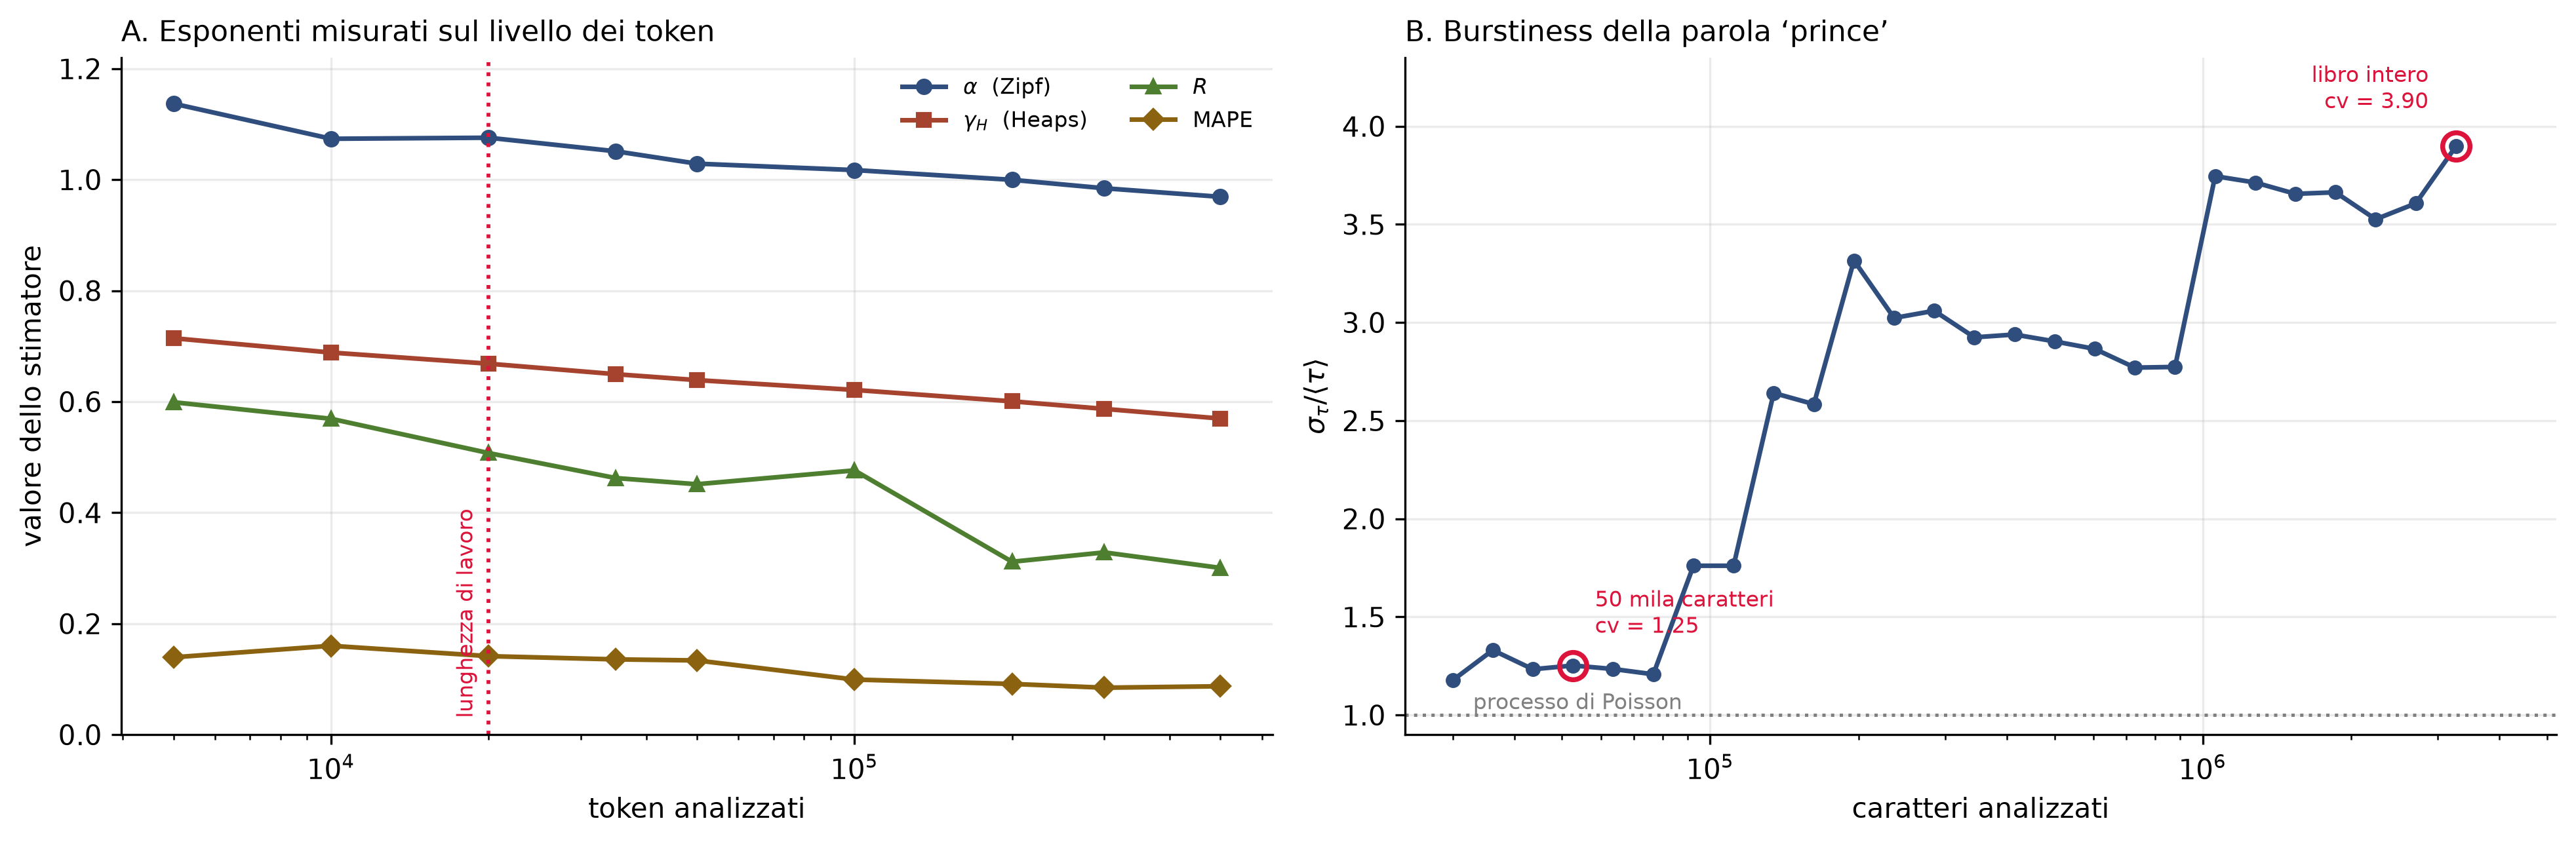
\includegraphics[width=\textwidth]{figure/cap3_dimensione_finita.png}
  \caption{Deriva degli stimatori con la lunghezza di analisi, misurata sulla
  continuazione di \emph{Guerra e pace} usata come baseline umana.
  \textbf{A}: gli esponenti misurati sul livello dei token decrescono tutti in
  modo monotono. Fra \num{5000} e \num{500000} token il descrittore $R$ passa da
  $0.60$ a $0.30$, dimezzandosi, mentre $\gamma_H$ scende da $0.72$ a $0.57$ e
  l'esponente di Zipf da $1.14$ a $0.97$. La linea verticale segna la lunghezza
  di lavoro adottata nei capitoli sperimentali.
  \textbf{B}: il coefficiente di variazione degli intervalli fra occorrenze
  della parola \emph{prince} cresce da $1.25$ su \num{50000} caratteri a $3.90$
  sul romanzo intero. La deriva è quella attesa quando la coda non
  presenta un taglio dentro la finestra osservata: finestre più lunghe
  campionano vuoti più lunghi, e la stima di $\sigma_\tau$ non raggiunge un
  valore limite. Il §\ref{sec:coda-risultati} misura direttamente il taglio e lo
  trova crescere con la finestra, da $13.5$ a $94.7$ intervalli medi fra
  \num{30000} e \num{480000} caratteri: i momenti sono finiti a ogni lunghezza,
  ma il loro valore dipende da essa.
  La Figura~\ref{fig:heaps-finito} mostrava lo stesso fenomeno su un solo
  stimatore ma su tre opere diverse, stabilendone l'universalità; qui il
  confronto è ristretto a un'unica opera e serve invece a quantificare l'entità
  dell'effetto sulla baseline effettivamente impiegata.}
  \label{fig:dimensione-finita}
\end{figure}

L'entità della deriva rende obbligatorie tre precauzioni operative, che valgono
per l'intero lavoro. Tutti i confronti fra corpora vengono condotti alla stessa
lunghezza di analisi, indicata d'ora in avanti con $N_{\mathrm{eff}}$ e
dichiarata per ciascuna fase, poiché non tutte le analisi condividono gli stessi
corpora. Nessun valore assoluto viene confrontato con valori pubblicati misurati
su lunghezze diverse. E ogni riferimento umano viene misurato con le stesse
procedure e alla stessa lunghezza dei testi con cui viene confrontato, anziché
ripreso dalla letteratura: è il paragrafo che segue. Il pannello B mostra il caso
concreto in cui la prima e la seconda precauzione si incontrano, cioè perché il
confronto con il valore pubblicato per \emph{prince} vada condotto sul romanzo
intero e non sui segmenti: è la stessa quantità, misurata su finestre che
differiscono di un fattore sessanta.

Per l'analisi appaiata dei corpora enciclopedici $N_{\mathrm{eff}}$ è fissato a
\num{60000} caratteri. Il valore è il massimo compatibile con la conservazione
di tutte le 39 terne: portandolo a \num{80000} quattro articoli non
raggiungono la soglia e le terne disponibili scendono da 39 a 35. L'intera
catena viene comunque ripetuta a quella lunghezza maggiore come controllo di
robustezza, il cui esito è riportato nel §\ref{sec:robustezza-neff} e distingue
le parti del divario che resistono al cambio di finestra da quelle che non vi
resistono.

Le altre fasi dell'analisi impiegano lunghezze diverse, perché non condividono i
corpora e non sono confrontate fra loro. La Tabella~\ref{tab:fasi} le riassume:
ciascun valore numerico che comparirà nei capitoli sperimentali è riconducibile
a una di queste righe.

\begin{table}[htbp]
\centering
\small
\begin{tabular}{@{}>{\raggedright\arraybackslash}p{2.9cm}>{\raggedright\arraybackslash}p{4.3cm}rll@{}}
\toprule
Fase & Scopo & $N_{\mathrm{eff}}$ & Unità & Analizzate \\
\midrule
Sweep di temperatura & misure sul corpus generato
  & \num{20000} & token & 242 documenti \\
\addlinespace
Raccolta & appaiamento per titolo e verifica di paternità
  & \num{80000} & caratteri & 40 coppie \\
\addlinespace
Fattibilità & verificare che l'effetto esista in prosa enciclopedica, senza
  Grokipedia & \num{50000} & caratteri & 40 voci, 20 segmenti \\
\addlinespace
Analisi principale & confronto appaiato fra i quattro corpora
  & \num{60000} & caratteri & 39 terne \\
\addlinespace
Robustezza & ripetizione dell'intera catena a lunghezza maggiore
  & \num{80000} & caratteri & 35 terne \\
\bottomrule
\end{tabular}
\caption{Le fasi dell'analisi e le rispettive lunghezze. I valori differiscono
perché le fasi non condividono i corpora, e la prima riga adotta una unità
diversa dalle altre per la ragione discussa nel §\ref{sec:unita}. Nessun
confronto attraversa righe diverse della tabella: la fase di fattibilità non
include Grokipedia, e quella sullo sweep non include alcun corpus
enciclopedico.}
\label{tab:fasi}
\end{table}

\paragraph{Baseline umana misurata, non citata.}
Per la stessa ragione, il riferimento umano non viene ripreso dalla letteratura
ma misurato con le stesse procedure e alla stessa lunghezza dei testi generati.
Il testo di riferimento è la continuazione del passaggio usato come prompt: il
confronto è quindi fra continuazione umana e continuazione generata, a parità di
contesto. La Tabella~\ref{tab:baseline} riporta i valori così ottenuti.

\begin{table}[htbp]
\centering
\small
\begin{tabular}{@{}lrr@{}}
\toprule
Grandezza & Misurata qui & Pubblicata \\
\midrule
$\alpha$ (Zipf)                 & 1.076  & $1.006 \pm 0.05$ \\
MAPE                            & 0.141  & $0.156 \pm 0.077$ \\
$\gamma_H$ (Heaps)              & 0.668  & $0.801 \pm 0.02$ \\
$R$                             & 0.507  & $0.17 \pm 0.05$ \\
$\alpha_{\mathrm{DFA}}$         & 0.579  & --- \\
$R_{\mathrm{gzip}}$             & 0.381  & --- \\
entropia [bit/carattere]        & 2.227  & --- \\
\bottomrule
\end{tabular}
\caption{Baseline umana misurata su \num{20000} token di \emph{Guerra e pace},
confrontata con i valori pubblicati in~\cite{mikhaylovskiy2025zipf}. Questi
ultimi sono calcolati su opere intere e non costituiscono un riferimento valido
per testi di questa lunghezza, per la ragione discussa nel
§\ref{sec:validazione}.}
\label{tab:baseline}
\end{table}

\paragraph{Appaiamento in frequenza dei controlli.}
Nel confronto fra parole di contenuto e parole di controllo, ciascun sostantivo
viene appaiato alla parola non-sostantivo di frequenza più vicina, minimizzando
$\lvert\log(f_w/f_k)\rvert$. L'appaiamento è indispensabile perché la burstiness
dipende dalla frequenza: confrontare parole di frequenza diversa misurerebbe
quella differenza anziché la natura semantica delle parole.

\paragraph{Selezione dei bersagli entro ciascun testo.}
Le parole bersaglio vengono scelte all'interno di ogni documento anziché fissate
una volta per tutte sul corpus di riferimento. La scelta è necessaria perché
corpora diversi trattano argomenti diversi e non condividono il lessico
tematico, ed è inoltre più efficiente, poiché produce un numero maggiore di
confronti appaiati a parità di corpus.

\paragraph{Come vengono separati i livelli lessicali.}
\label{par:livelli-lessicali}
Dentro ciascun documento le parole vengono ordinate per frequenza e ripartite in
tre insiemi. Le \emph{parole funzione} sono le sei più frequenti fra quelle che
compaiono in una lista chiusa di funtori inglesi. Le \emph{parole chiave} sono
le sette più frequenti fra quelle che superano i quattro caratteri e non
figurano in quella lista, oppure che risultano nomi propri per il criterio di
maiuscola in posizione interna alla frase descritto sopra. I \emph{controlli
appaiati} sono, per ciascuna parola chiave, la parola di frequenza più vicina
fra quelle rimaste. La ripartizione è dunque interamente determinata dalla lista
dei funtori, e la sua completezza è una scelta di metodo con conseguenze
misurabili.

La lista impiegata inizialmente conteneva \num{133} voci e ometteva alcuni
connettivi e attenuatori inglesi molto comuni, fra cui \emph{like},
\emph{amid}, \emph{including}, \emph{though}, \emph{also}, \emph{rather} e
\emph{without}. In un corpus in cui quei termini restano rari l'omissione è
innocua; in Grokipedia non lo è, perché il testo generato li impiega molto più
spesso: \emph{like} entrava fra le sette parole più frequenti in \num{29} voci
su \num{39}, contro nessuna di Wikipedia. Finivano quindi classificati come
parole chiave. Poiché i connettivi ricorrono a cadenza quasi costante e hanno
perciò burstiness bassa, il livello lessicale alto di Grokipedia risultava
contaminato da materiale che appartiene al livello dei funtori, e il divario
misurato a quel livello ne usciva gonfiato.

La lista è stata quindi estesa a \num{215} voci per classe grammaticale, cioè
preposizioni, congiunzioni subordinanti, avverbi connettivi e attenuatori e
quantificatori, e applicata identica a tutti e quattro i corpora. L'estensione
non rimuove nulla: le parole interessate passano al livello dei funtori, e al
loro posto sale fra le parole chiave la parola di contenuto successiva in
ordine di frequenza, cosicché tutti i livelli conservano la stessa numerosità
in tutti i corpora. Tutte le misure del Capitolo~\ref{cap:risultati2} sono
calcolate con la lista estesa; il §\ref{sec:effetto-stoplist} riporta di
quanto si spostano i risultati, perché lo spostamento non è trascurabile e la
scelta va resa verificabile.

% ---------------------------------------------------------------------
\section{Validazione delle procedure di calcolo}
\label{sec:validazione}

Ogni conclusione di questo lavoro poggia sul fatto che il codice misuri
effettivamente le quantità definite nel Capitolo~\ref{cap:teoria}. La
validazione procede per due vie indipendenti: la riproduzione di valori
pubblicati e la misura di grandezze il cui valore esatto è noto per costruzione.

\paragraph{Riproduzione di valori pubblicati.}
Le quantità del protocollo di Altmann sono state misurate sul corpus letterario
e confrontate con quelle riportate in~\cite{altmann2012}. Il null model A1, che
per costruzione deve restituire $\hat\gamma_{A1} \simeq 1$, dà valori compresi
fra $0.972$ e $0.984$ ai quattro livelli linguistici esaminati.

La seconda quantità riprodotta è il coefficiente di variazione della parola
\emph{prince}, che vale $3.89$ sul libro intero, in accordo con il $3.86$
pubblicato, ma scende a $1.30$ sui segmenti da \num{50000} caratteri impiegati
nei confronti. Non si tratta di un disaccordo: è la deriva di dimensione finita del
§\ref{sec:lunghezza}, e mostra perché i valori assoluti non vadano confrontati
fra lunghezze diverse. Il confronto con il valore pubblicato è quindi condotto
sul libro intero, mentre i confronti fra corpora usano la lunghezza comune.

\paragraph{Misura di esponenti noti.}
La seconda via non dipende da alcuna pubblicazione. Le procedure sono state
applicate a segnali costruiti in modo che il risultato atteso sia noto
analiticamente, ottenendo i valori della Tabella~\ref{tab:validazione}.

\begin{table}[htbp]
\centering
\small
\begin{tabular}{@{}l>{\raggedright\arraybackslash}p{5.6cm}rr@{}}
\toprule
Procedura & Segnale di prova & Atteso & Ottenuto \\
\midrule
DFA & rumore bianco & 0.500 & 0.510 \\
DFA & cammino aleatorio & 1.500 & 1.494 \\
Stimatore KL & testo confrontato con sé stesso & 0 & $0$ esatto \\
Stimatore KL & due campioni della stessa sorgente & $\simeq 0$ & 0.001 \\
Stimatore KL & sorgenti diverse & $> 0$ & 0.687 \\
\bottomrule
\end{tabular}
\caption{Validazione su segnali a esponente noto. Le prime due righe verificano
l'esponente della detrended fluctuation analysis; le ultime tre verificano che
lo stimatore della divergenza di Kullback--Leibler si annulli esattamente sul
confronto di un testo con sé stesso, resti prossimo a zero fra campioni della
stessa sorgente e cresca fra sorgenti diverse.}
\label{tab:validazione}
\end{table}

La proprietà $D(x\|x) = 0$ non è un accordo approssimato ma un'identità esatta,
e costituisce il controllo più stringente sullo stimatore della divergenza:
come discusso nel §\ref{sec:crossparsing}, essa vale soltanto se i riferimenti
usati nei due termini hanno la stessa lunghezza, e una sua violazione
segnalerebbe immediatamente l'errore.

% ---------------------------------------------------------------------
\section{Controlli di robustezza}
\label{sec:robustezza}

I controlli di questa sezione non verificano che le procedure siano corrette, ma
che i risultati non dipendano da scelte che avrebbero potuto essere compiute
diversamente.

\paragraph{Ordine del detrending.}
La detrended fluctuation analysis rimuove dalle finestre le tendenze polinomiali
fino a un grado fissato. L'intera analisi è stata condotta con il grado 1 e con
il grado 2, e la Tabella~\ref{tab:ordine-dfa} riporta le due stime a ciascuna
temperatura. Le misure riportate nel Capitolo~\ref{cap:risultati1} usano il
grado 2, per la ragione che il confronto stesso rende evidente: dove il segnale
è stazionario i due gradi coincidono, e dove non lo è il grado 1 restituisce un
esponente sistematicamente più alto, perché lascia nel segnale una tendenza che
non è correlazione.

\begin{table}[htbp]
\centering
\small
\begin{tabular}{@{}lrrrrr@{}}
\toprule
$T$ & grado 1 & grado 2 & scarto & dispersione & documenti \\
\midrule
0.4 & 0.284 & 0.307 & $-0.046$ & 0.085 & 21 \\
0.5 & 0.582 & 0.500 & $-0.132$ & 0.081 & 21 \\
0.6 & 0.613 & 0.416 & $-0.124$ & 0.093 & 21 \\
0.7 & 0.713 & 0.583 & $-0.115$ & 0.073 & 21 \\
0.8 & 0.715 & 0.601 & $-0.138$ & 0.070 & 20 \\
0.9 & 0.758 & 0.659 & $-0.078$ & 0.050 & 18 \\
1.0 & 0.753 & 0.711 & $-0.014$ & 0.054 & 17 \\
1.1 & 0.651 & 0.564 & $-0.060$ & 0.046 & 19 \\
1.2 & 0.570 & 0.556 & $-0.029$ & 0.035 & 21 \\
1.3 & 0.563 & 0.535 & $-0.007$ & 0.024 & 21 \\
1.4 & 0.535 & 0.532 & $-0.009$ & 0.019 & 21 \\
1.5 & 0.529 & 0.527 & $-0.006$ & 0.015 & 21 \\
\midrule
\multicolumn{3}{@{}l}{testo umano} & $-0.007$ & --- & 1 \\
\bottomrule
\end{tabular}
\caption{Esponente della fluttuazione stimato con detrending di grado 1 e di
grado 2. Le prime tre colonne numeriche riportano mediane sui documenti
disponibili a ciascuna temperatura; la quarta è la deviazione standard dello
scarto fra i due gradi, calcolata documento per documento. Lo scarto è negativo
ovunque, come atteso, perché il grado 2 rimuove tendenze che il grado 1 lascia
nel segnale.}
\label{tab:ordine-dfa}
\end{table}

Le due stime coincidono dove il segnale è stazionario. Sulla baseline umana lo
scarto vale $-0.007$, e sui testi generati da $T = 1.2$ in su la sua mediana vale
$-0.010$ a fronte di una dispersione fra documenti di $0.027$: la differenza fra
i due gradi è più piccola della variabilità fra documenti generati nelle stesse
condizioni, e l'esponente non dipende in modo apprezzabile dalla scelta del
detrending.

Nell'intervallo $T \in [0.5, 0.8]$ lo scarto mediano vale invece $-0.125$, con
dispersione $0.078$: qui la differenza supera nettamente la variabilità ed è
quindi reale. È concentrata nel regime in cui il testo degenera in cicli di
ripetizione e la serie dei ranghi non è stazionaria, e in quel regime,
coerentemente con quanto osservato nel §\ref{sec:ponte}, l'esponente va letto
come indicatore di periodicità e non come misura di correlazione a lungo raggio.


\paragraph{Numerosità disuguale fra celle.}
Dalla disuguale numerosità dichiarata nel §\ref{sec:protocollo} discendono due
limitazioni. Per il modello da 14 miliardi di parametri non esiste una stima
della dispersione fra campioni, cosicché nelle sue figure le barre d'errore non
sono definite e ogni suo valore è una singola realizzazione; e le deviazioni
standard riportate nelle figure del Capitolo~\ref{cap:risultati1} non sono
confrontabili fra modelli, poiché derivano da un numero diverso di campioni. Le
conclusioni che riguardano il confronto fra modelli vanno lette con questa
avvertenza, che il §\ref{sec:zipf-risultati} riprende quantitativamente sul
caso in cui pesa di più.

% ---------------------------------------------------------------------
\section{Riproducibilità}
\label{sec:riproducibilita}

Tutte le procedure sono deterministiche a semi fissati, e i semi impiegati sono
registrati nel codice. I corpora scaricati da fonti esterne sono conservati in
copia locale, così che una modifica successiva della fonte non alteri i
risultati: vale in particolare per le voci di Grokipedia, che vengono riscritte
senza cronologia pubblica.

I dati intermedi e le figure sono prodotti da notebook che salvano ogni risultato
in file separati, in formato aperto, insieme a una sintesi testuale dei
parametri usati e delle scelte compiute, così che ciascuna figura sia
ricostruibile senza ripetere i calcoli.

% =====================================================================

\chapter{Materiali e metodi}
\label{cap:metodi}

Questo capitolo descrive i corpora analizzati, il protocollo con cui i testi
artificiali sono stati prodotti e le scelte metodologiche comuni alle due parti
sperimentali. Il criterio seguito nell'esposizione è che un lettore debba poter
ripetere l'intera analisi senza dover chiedere nulla: ogni scelta viene perciò
motivata e non soltanto dichiarata.

Le ultime tre sezioni sono dedicate ai controlli. Il §\ref{sec:validazione}
verifica che le procedure di calcolo misurino effettivamente le quantità
definite nel Capitolo~\ref{cap:teoria}; il §\ref{sec:robustezza} verifica che i
risultati non dipendano da scelte arbitrarie. Sono due questioni distinte, e
tenerle separate rende più chiaro che cosa ciascun controllo dimostri.

% ---------------------------------------------------------------------
\section{I corpora}
\label{sec:corpora}

L'analisi impiega cinque corpora, riassunti nella Tabella~\ref{tab:corpora}.
Due sono di riferimento umano, due sono enciclopedie messe a confronto fra loro,
e uno raccoglie i testi generati automaticamente.

\begin{table}[htbp]
\centering
\small
\begin{tabular}{@{}l>{\raggedright\arraybackslash}p{5.9cm}c@{}}
\toprule
Corpus & Provenienza e criterio di selezione & Unità \\
\midrule
\emph{Guerra e pace} & Project Gutenberg; segmenti contigui di uguale lunghezza,
usati come ancora al protocollo originale & 20 segmenti \\
\addlinespace
Wikipedia & voci a tema ampio, selezionate ordinando per lunghezza di prosa
effettiva & 40 raccolte, 39 analizzate \\
\addlinespace
Grokipedia (attuale) & le stesse voci, appaiate per titolo & 40 raccolte, 39
analizzate \\
\addlinespace
Grokipedia v0.1 & le stesse voci nella versione di ottobre 2025, recuperata da
Internet Archive & 40 raccolte, 39 analizzate \\
\addlinespace
Testi generati & cinque modelli Qwen, sweep di temperatura descritto nel
§\ref{sec:protocollo} & 242 documenti \\
\bottomrule
\end{tabular}
\caption{I corpora analizzati.}
\label{tab:corpora}
\end{table}

Il corpus letterario ha una funzione precisa: fornire un'ancora al protocollo di
Altmann~\cite{altmann2012}, che è stato formulato e validato su romanzi. I valori
misurati su di esso permettono di verificare che la procedura riproduca quanto
pubblicato prima di applicarla a testi di natura diversa.

Le voci di Wikipedia sono state ordinate per lunghezza del solo testo corrente,
dopo rimozione di marcatura, tabelle, note e riferimenti. I due criteri più
immediati non sono utilizzabili. Ordinare le pagine per dimensione del sorgente
wiki restituisce liste, tabelle e infobox anziché prosa: una pagina da
\num{679016} byte di sorgente conteneva \num{1284} caratteri di prosa effettiva.
Ordinare per qualità editoriale è ugualmente inadatto, poiché le voci in vetrina
sono selezionate per accuratezza e non per lunghezza.

Grokipedia compare in due versioni perché la piattaforma non pubblica una
cronologia delle revisioni. La versione di ottobre 2025 è stata recuperata da
Internet Archive, disponibile per tutte e quaranta le voci, e consente di
verificare se gli indicatori misurati cambino a seguito della revisione
editoriale: è il controllo riportato nel Capitolo~\ref{cap:risultati2}.

% ---------------------------------------------------------------------
\section{Protocollo di generazione}
\label{sec:protocollo}

I testi artificiali sono stati prodotti da cinque modelli della famiglia Qwen,
elencati nella Tabella~\ref{tab:modelli}. Tutti sono modelli \emph{base}, cioè
non sottoposti ad affinamento su istruzioni: la scelta isola le proprietà del
modello linguistico da quelle indotte dall'addestramento successivo, che
in~\cite{mikhaylovskiy2025zipf} risultano spostare sensibilmente il
comportamento statistico.

\begin{table}[htbp]
\centering
\small
\begin{tabular}{@{}llrlr@{}}
\toprule
Modello & Famiglia & Parametri & Architettura & Documenti \\
\midrule
Qwen2.5-1.5B     & Qwen2.5 & 1.54\,G  & transformer denso & 57 \\
Qwen2.5-3B       & Qwen2.5 & 3.09\,G  & transformer denso & 53 \\
Qwen2.5-14B      & Qwen2.5 & 14.7\,G  & transformer denso & 12 \\
Qwen3.5-2B-Base  & Qwen3.5 & 2.0\,G   & ibrida            & 60 \\
Qwen3.5-4B-Base  & Qwen3.5 & 4.0\,G   & ibrida            & 60 \\
\midrule
\multicolumn{4}{@{}l}{totale} & 242 \\
\bottomrule
\end{tabular}
\caption{I cinque modelli impiegati. L'intervallo di dimensioni copre un ordine
di grandezza, e le due famiglie differiscono per architettura. I modelli
Qwen2.5 sono transformer densi ad attenzione completa su tutti gli strati; i
modelli Qwen3.5 sono ibridi e ripetono un blocco di quattro strati in cui tre
impiegano attenzione lineare e uno attenzione completa. Le schede ufficiali
riportano \num{24} strati per il modello da 2 miliardi di parametri, come
$6\times(3\times\text{lineare} + 1\times\text{completa})$, e \num{32} per
quello da 4 miliardi, come $8\times(3+1)$: in entrambi i casi tre quarti degli
strati sono ad attenzione lineare.}
\label{tab:modelli}
\end{table}

Ogni modello ha generato testo a dodici temperature, da $T = 0.4$ a $T = 1.5$
con passo $0.1$. Il prompt è identico per tutti: un blocco di 2000 token tratto
da \emph{Guerra e pace}, la cui posizione esatta nel romanzo è stata verificata
come descritto nel §\ref{sec:paternita}. Ciascuna generazione produce
\num{24000} token di completamento, misurati con il tokenizzatore del modello
generante.

\paragraph{Che cosa comporta un prompt lungo.}
La scelta di un prompt di 2000 token non è neutra rispetto alle misure, e la
conseguenza è anticipata qui perché ricorre in tutto il
Capitolo~\ref{cap:risultati1}. La sezione 4.5
di~\cite{mikhaylovskiy2025zipf} ripete lo sweep con un prompt di quella
lunghezza tratto da un testo naturale e osserva che la ricchezza lessicale del
prompt domina il vocabolario, relativamente piccolo, del testo generato: alcuni
modelli non producono alcun tipo nuovo alle basse temperature, i massimi delle
curve del descrittore $R$ si spostano verso le temperature alte, e l'errore del
fit di Zipf si abbassa soprattutto nella regione a bassa temperatura. Le
proprietà del regime disordinato compaiono dunque più tardi, e quelle del
regime ordinato persistono più a lungo, di quanto si osserverebbe generando da
un singolo token. I confronti con i valori pubblicati vanno letti tenendone
conto, e i punti in cui l'effetto si manifesta sono segnalati di volta in
volta.

Il campionamento impiega la sola temperatura. I parametri che troncano la
distribuzione sono disattivati, con $\mathrm{top}\text{-}p = 1$ e
$\mathrm{top}\text{-}k = -1$, e la penalità di ripetizione è posta a 1. È la
condizione richiesta dal §\ref{sec:temperatura}: qualunque altro parametro
introdurrebbe un secondo grado di libertà e renderebbe impossibile attribuire
alla sola temperatura il comportamento osservato.

\paragraph{Generazione in continuazione.}
Per raggiungere i \num{24000} token richiesti la generazione riparte dopo ogni
token di fine sequenza, riprendendo dal testo accumulato fino a quel punto. I
documenti prodotti sono dunque ricuciti da più segmenti, in numero variabile fino
a un massimo di 27 riprese per campione. Poiché un modello autoregressivo è privo
di stato interno persistente, riprendere dal testo accumulato produce la stessa
distribuzione condizionata. Un confronto a temperatura fissata fra i documenti
ricuciti da più segmenti e quelli generati in un colpo solo non rivela
differenze nelle due misure sensibili all'ordine, entro la dispersione dei dati;
il confronto ha però poca potenza, perché sotto $T = 0.9$ i documenti con
riprese sono pochissimi e sopra $T = 1.0$ la ripetizione è già nulla.

\paragraph{Numerosità disuguale.}
Il numero di documenti per modello non è uniforme, e la
Tabella~\ref{tab:modelli} lo riporta esplicitamente: il modello da 14 miliardi
di parametri dispone di un solo campione per temperatura, contro i cinque della
maggior parte degli altri. Le conseguenze sono discusse fra i limiti nel
§\ref{sec:robustezza}.

% ---------------------------------------------------------------------
\section{Verifica di paternità dei corpora}
\label{sec:paternita}

Il confronto fra Wikipedia e Grokipedia presuppone che le voci della seconda
siano effettivamente scritte da un modello generativo e non ricopiate dalla
prima. La verifica misura la sovrapposizione di 8-grammi fra le due versioni di
ciascuna voce: sul corpus attuale la mediana vale $0.0003$ e il massimo $0.046$,
valori che escludono la derivazione testuale diretta. Una voce della versione
v0.1, \emph{Buddhism}, risultava invece ricopiata all'84\% ed è stata esclusa
dall'analisi appaiata, che si riduce quindi a 39 terne: il disegno richiede
infatti che tutte e tre le versioni siano disponibili per ogni titolo, per cui
l'esclusione di una versione comporta quella dell'intera terna.

Per i testi generati la verifica riguarda il prompt. Poiché i cinque dataset sono
stati prodotti in momenti diversi, occorre accertare che partano tutti dallo
stesso punto del romanzo. Il controllo non è stato condotto per ispezione ma per
funzione di hash: dell'impronta SHA-256 registrata in ciascun dataset è stata
cercata la corrispondenza nel testo del romanzo, individuando l'offset esatto in
caratteri. Tutti e cinque i dataset risultano partire dalla stessa posizione. Due
di essi registrano una lunghezza del prompt di poco diversa, \num{8239} contro
\num{8262} caratteri, differenza dovuta al punto in cui cade il confine dei 2000
token con i due tokenizzatori delle rispettive famiglie e non a un testo diverso.

% ---------------------------------------------------------------------
\section{Unità di analisi}
\label{sec:unita}

La scelta dell'unità in cui misurare i testi è la decisione metodologica di
maggiore conseguenza dell'intero lavoro, e viene qui motivata per esteso.

Il livello primario è il token, non la parola. La ragione, già anticipata nel
§\ref{sec:token}, è che alle temperature alte i modelli producono sequenze non
interpretabili come parole: una tokenizzazione lessicale misurerebbe in quel
regime artefatti della segmentazione anziché proprietà del testo. La stessa
scelta, e per lo stesso motivo, è compiuta in~\cite{mikhaylovskiy2025zipf}.

Il tokenizzatore impiegato nell'analisi è unico per tutti i corpora ed è esterno
alle famiglie che hanno generato i testi. Le due condizioni sono entrambe
necessarie. L'unicità serve a rendere confrontabili gli esponenti misurati su
modelli diversi: i tokenizzatori di Qwen2.5 e Qwen3.5 segmentano lo stesso testo
in modo diverso, e misurare ciascun modello con il proprio metro produrrebbe
differenze attribuibili alla segmentazione anziché al testo. L'esternalità serve
a evitare che un modello risulti favorito dal fatto di essere misurato con il
proprio vocabolario. La scelta ricalca quella di~\cite{mikhaylovskiy2025zipf},
dove testi prodotti da quattro famiglie distinte vengono analizzati con un
tokenizzatore che non appartiene a nessuna di esse.

In concreto l'analisi impiega \texttt{cl100k\_base}, con \num{100277} voci.
Cambiare tokenizzatore sposta i valori assoluti degli esponenti, poiché cambia
l'unità in cui si contano le occorrenze, ma non la posizione dei loro estremi in
funzione della temperatura, che è la quantità su cui poggiano le conclusioni del
Capitolo~\ref{cap:risultati1}.

Ogni documento generato viene troncato ai primi \num{20000} token di analisi, e
la baseline umana è misurata sulla stessa quantità. Il valore è il massimo
compatibile con il documento più corto del corpus: la generazione produce
\num{24000} token misurati con il tokenizzatore del modello generante, che
\texttt{cl100k\_base} risegmenta in un numero variabile di token di analisi, e
troncare a una soglia comune è indispensabile perché tutte le misure del
Capitolo~\ref{cap:risultati1} dipendono dalla lunghezza. La prima riga della
Tabella~\ref{tab:fasi} riporta questa fase; le altre adottano il carattere come
unità, perché il protocollo del §\ref{sec:burst} misura le distanze in
caratteri.

Il livello lessicale resta impiegato, in funzione secondaria, per le misure che
sono definite sulle parole: la diversità lessicale, le distanze di ripetizione,
gli $n$-grammi ripetuti e la mappatura sui vettori di embedding. La detrended
fluctuation analysis fa eccezione a entrambi i livelli, poiché
in~\cite{lippi2019} è definita sui caratteri, e qui si segue quella definizione.

% ---------------------------------------------------------------------
\section{Scelte metodologiche trasversali}
\label{sec:scelte}

Quattro decisioni attraversano entrambe le parti sperimentali.

\paragraph{Lunghezza di analisi comune.}
Come anticipato nel §\ref{sec:lunghezza}, diversi stimatori impiegati in questo
lavoro non convergono al crescere della lunghezza del testo, ma derivano in modo
sistematico. La Figura~\ref{fig:dimensione-finita} misura la deriva su un testo
umano, e mostra che non si tratta di un effetto trascurabile.

\begin{figure}[htbp]
  \centering
  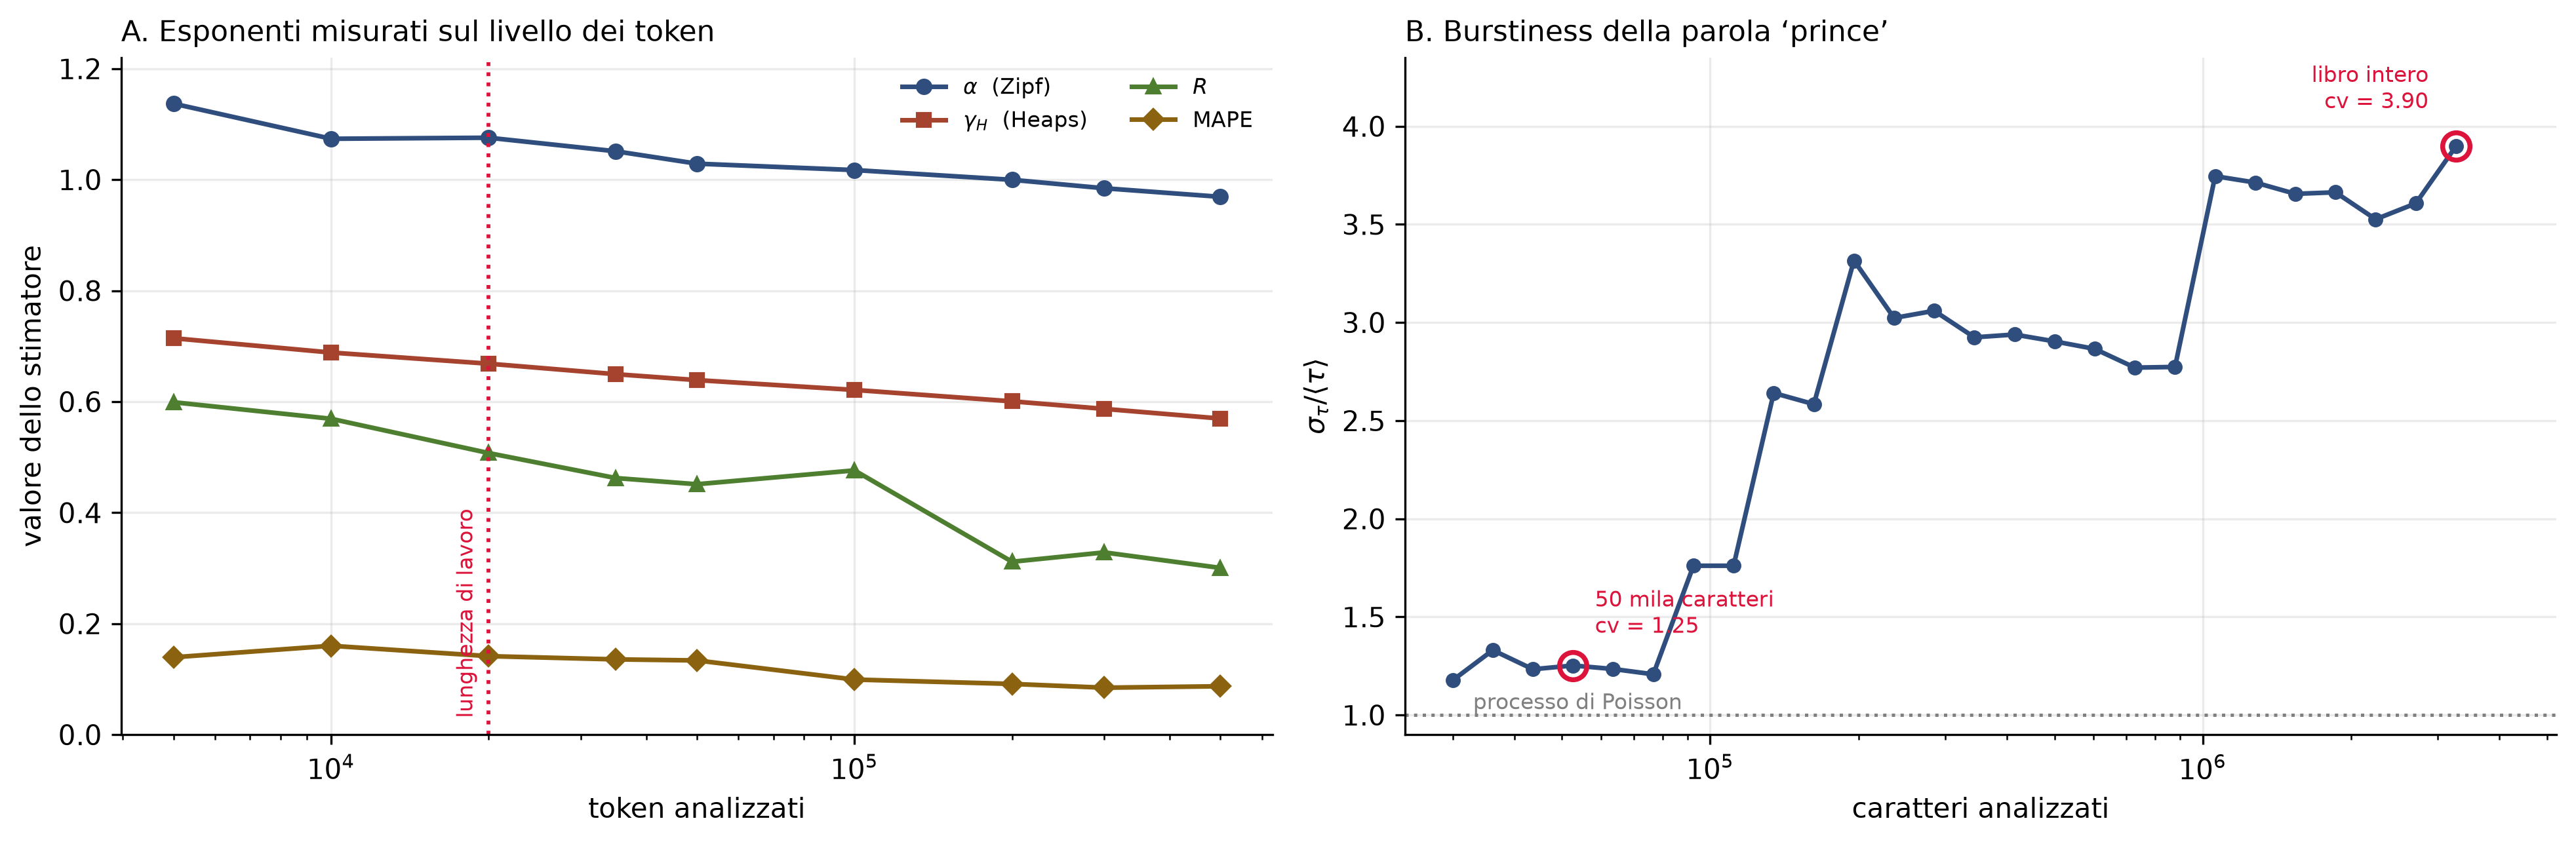
\includegraphics[width=\textwidth]{figure/cap3_dimensione_finita.png}
  \caption{Deriva degli stimatori con la lunghezza di analisi, misurata sulla
  continuazione di \emph{Guerra e pace} usata come baseline umana.
  \textbf{A}: gli esponenti misurati sul livello dei token decrescono tutti in
  modo monotono. Fra \num{5000} e \num{500000} token il descrittore $R$ passa da
  $0.60$ a $0.30$, dimezzandosi, mentre $\gamma_H$ scende da $0.72$ a $0.57$ e
  l'esponente di Zipf da $1.14$ a $0.97$. La linea verticale segna la lunghezza
  di lavoro adottata nei capitoli sperimentali.
  \textbf{B}: il coefficiente di variazione degli intervalli fra occorrenze
  della parola \emph{prince} cresce da $1.25$ su \num{50000} caratteri a $3.90$
  sul romanzo intero. La deriva è quella attesa quando la coda non
  presenta un taglio dentro la finestra osservata: finestre più lunghe
  campionano vuoti più lunghi, e la stima di $\sigma_\tau$ non raggiunge un
  valore limite. Il §\ref{sec:coda-risultati} misura direttamente il taglio e lo
  trova crescere con la finestra, da $13.5$ a $94.7$ intervalli medi fra
  \num{30000} e \num{480000} caratteri: i momenti sono finiti a ogni lunghezza,
  ma il loro valore dipende da essa.
  La Figura~\ref{fig:heaps-finito} mostrava lo stesso fenomeno su un solo
  stimatore ma su tre opere diverse, stabilendone l'universalità; qui il
  confronto è ristretto a un'unica opera e serve invece a quantificare l'entità
  dell'effetto sulla baseline effettivamente impiegata.}
  \label{fig:dimensione-finita}
\end{figure}

L'entità della deriva rende obbligatorie tre precauzioni operative, che valgono
per l'intero lavoro. Tutti i confronti fra corpora vengono condotti alla stessa
lunghezza di analisi, indicata d'ora in avanti con $N_{\mathrm{eff}}$ e
dichiarata per ciascuna fase, poiché non tutte le analisi condividono gli stessi
corpora. Nessun valore assoluto viene confrontato con valori pubblicati misurati
su lunghezze diverse. E ogni riferimento umano viene misurato con le stesse
procedure e alla stessa lunghezza dei testi con cui viene confrontato, anziché
ripreso dalla letteratura: è il paragrafo che segue. Il pannello B mostra il caso
concreto in cui la prima e la seconda precauzione si incontrano, cioè perché il
confronto con il valore pubblicato per \emph{prince} vada condotto sul romanzo
intero e non sui segmenti: è la stessa quantità, misurata su finestre che
differiscono di un fattore sessanta.

Per l'analisi appaiata dei corpora enciclopedici $N_{\mathrm{eff}}$ è fissato a
\num{60000} caratteri. Il valore è il massimo compatibile con la conservazione
di tutte le 39 terne: portandolo a \num{80000} quattro articoli non
raggiungono la soglia e le terne disponibili scendono da 39 a 35. L'intera
catena viene comunque ripetuta a quella lunghezza maggiore come controllo di
robustezza, il cui esito è riportato nel §\ref{sec:robustezza-neff} e distingue
le parti del divario che resistono al cambio di finestra da quelle che non vi
resistono.

Le altre fasi dell'analisi impiegano lunghezze diverse, perché non condividono i
corpora e non sono confrontate fra loro. La Tabella~\ref{tab:fasi} le riassume:
ciascun valore numerico che comparirà nei capitoli sperimentali è riconducibile
a una di queste righe.

\begin{table}[htbp]
\centering
\small
\begin{tabular}{@{}>{\raggedright\arraybackslash}p{2.9cm}>{\raggedright\arraybackslash}p{4.3cm}rll@{}}
\toprule
Fase & Scopo & $N_{\mathrm{eff}}$ & Unità & Analizzate \\
\midrule
Sweep di temperatura & misure sul corpus generato
  & \num{20000} & token & 242 documenti \\
\addlinespace
Raccolta & appaiamento per titolo e verifica di paternità
  & \num{80000} & caratteri & 40 coppie \\
\addlinespace
Fattibilità & verificare che l'effetto esista in prosa enciclopedica, senza
  Grokipedia & \num{50000} & caratteri & 40 voci, 20 segmenti \\
\addlinespace
Analisi principale & confronto appaiato fra i quattro corpora
  & \num{60000} & caratteri & 39 terne \\
\addlinespace
Robustezza & ripetizione dell'intera catena a lunghezza maggiore
  & \num{80000} & caratteri & 35 terne \\
\bottomrule
\end{tabular}
\caption{Le fasi dell'analisi e le rispettive lunghezze. I valori differiscono
perché le fasi non condividono i corpora, e la prima riga adotta una unità
diversa dalle altre per la ragione discussa nel §\ref{sec:unita}. Nessun
confronto attraversa righe diverse della tabella: la fase di fattibilità non
include Grokipedia, e quella sullo sweep non include alcun corpus
enciclopedico.}
\label{tab:fasi}
\end{table}

\paragraph{Baseline umana misurata, non citata.}
Per la stessa ragione, il riferimento umano non viene ripreso dalla letteratura
ma misurato con le stesse procedure e alla stessa lunghezza dei testi generati.
Il testo di riferimento è la continuazione del passaggio usato come prompt: il
confronto è quindi fra continuazione umana e continuazione generata, a parità di
contesto. La Tabella~\ref{tab:baseline} riporta i valori così ottenuti.

\begin{table}[htbp]
\centering
\small
\begin{tabular}{@{}lrr@{}}
\toprule
Grandezza & Misurata qui & Pubblicata \\
\midrule
$\alpha$ (Zipf)                 & 1.076  & $1.006 \pm 0.05$ \\
MAPE                            & 0.141  & $0.156 \pm 0.077$ \\
$\gamma_H$ (Heaps)              & 0.668  & $0.801 \pm 0.02$ \\
$R$                             & 0.507  & $0.17 \pm 0.05$ \\
$\alpha_{\mathrm{DFA}}$         & 0.579  & --- \\
$R_{\mathrm{gzip}}$             & 0.381  & --- \\
entropia [bit/carattere]        & 2.227  & --- \\
\bottomrule
\end{tabular}
\caption{Baseline umana misurata su \num{20000} token di \emph{Guerra e pace},
confrontata con i valori pubblicati in~\cite{mikhaylovskiy2025zipf}. Questi
ultimi sono calcolati su opere intere e non costituiscono un riferimento valido
per testi di questa lunghezza, per la ragione discussa nel
§\ref{sec:validazione}.}
\label{tab:baseline}
\end{table}

\paragraph{Appaiamento in frequenza dei controlli.}
Nel confronto fra parole di contenuto e parole di controllo, ciascun sostantivo
viene appaiato alla parola non-sostantivo di frequenza più vicina, minimizzando
$\lvert\log(f_w/f_k)\rvert$. L'appaiamento è indispensabile perché la burstiness
dipende dalla frequenza: confrontare parole di frequenza diversa misurerebbe
quella differenza anziché la natura semantica delle parole.

\paragraph{Selezione dei bersagli entro ciascun testo.}
Le parole bersaglio vengono scelte all'interno di ogni documento anziché fissate
una volta per tutte sul corpus di riferimento. La scelta è necessaria perché
corpora diversi trattano argomenti diversi e non condividono il lessico
tematico, ed è inoltre più efficiente, poiché produce un numero maggiore di
confronti appaiati a parità di corpus.

\paragraph{Come vengono separati i livelli lessicali.}
\label{par:livelli-lessicali}
Dentro ciascun documento le parole vengono ordinate per frequenza e ripartite in
tre insiemi. Le \emph{parole funzione} sono le sei più frequenti fra quelle che
compaiono in una lista chiusa di funtori inglesi. Le \emph{parole chiave} sono
le sette più frequenti fra quelle che superano i quattro caratteri e non
figurano in quella lista, oppure che risultano nomi propri per il criterio di
maiuscola in posizione interna alla frase descritto sopra. I \emph{controlli
appaiati} sono, per ciascuna parola chiave, la parola di frequenza più vicina
fra quelle rimaste. La ripartizione è dunque interamente determinata dalla lista
dei funtori, e la sua completezza è una scelta di metodo con conseguenze
misurabili.

La lista impiegata inizialmente conteneva \num{133} voci e ometteva alcuni
connettivi e attenuatori inglesi molto comuni, fra cui \emph{like},
\emph{amid}, \emph{including}, \emph{though}, \emph{also}, \emph{rather} e
\emph{without}. In un corpus in cui quei termini restano rari l'omissione è
innocua; in Grokipedia non lo è, perché il testo generato li impiega molto più
spesso: \emph{like} entrava fra le sette parole più frequenti in \num{29} voci
su \num{39}, contro nessuna di Wikipedia. Finivano quindi classificati come
parole chiave. Poiché i connettivi ricorrono a cadenza quasi costante e hanno
perciò burstiness bassa, il livello lessicale alto di Grokipedia risultava
contaminato da materiale che appartiene al livello dei funtori, e il divario
misurato a quel livello ne usciva gonfiato.

La lista è stata quindi estesa a \num{215} voci per classe grammaticale, cioè
preposizioni, congiunzioni subordinanti, avverbi connettivi e attenuatori e
quantificatori, e applicata identica a tutti e quattro i corpora. L'estensione
non rimuove nulla: le parole interessate passano al livello dei funtori, e al
loro posto sale fra le parole chiave la parola di contenuto successiva in
ordine di frequenza, cosicché tutti i livelli conservano la stessa numerosità
in tutti i corpora. Tutte le misure del Capitolo~\ref{cap:risultati2} sono
calcolate con la lista estesa; il §\ref{sec:effetto-stoplist} riporta di
quanto si spostano i risultati, perché lo spostamento non è trascurabile e la
scelta va resa verificabile.

% ---------------------------------------------------------------------
\section{Validazione delle procedure di calcolo}
\label{sec:validazione}

Ogni conclusione di questo lavoro poggia sul fatto che il codice misuri
effettivamente le quantità definite nel Capitolo~\ref{cap:teoria}. La
validazione procede per due vie indipendenti: la riproduzione di valori
pubblicati e la misura di grandezze il cui valore esatto è noto per costruzione.

\paragraph{Riproduzione di valori pubblicati.}
Le quantità del protocollo di Altmann sono state misurate sul corpus letterario
e confrontate con quelle riportate in~\cite{altmann2012}. Il null model A1, che
per costruzione deve restituire $\hat\gamma_{A1} \simeq 1$, dà valori compresi
fra $0.972$ e $0.984$ ai quattro livelli linguistici esaminati.

La seconda quantità riprodotta è il coefficiente di variazione della parola
\emph{prince}, che vale $3.89$ sul libro intero, in accordo con il $3.86$
pubblicato, ma scende a $1.30$ sui segmenti da \num{50000} caratteri impiegati
nei confronti. Non si tratta di un disaccordo: è la deriva di dimensione finita del
§\ref{sec:lunghezza}, e mostra perché i valori assoluti non vadano confrontati
fra lunghezze diverse. Il confronto con il valore pubblicato è quindi condotto
sul libro intero, mentre i confronti fra corpora usano la lunghezza comune.

\paragraph{Misura di esponenti noti.}
La seconda via non dipende da alcuna pubblicazione. Le procedure sono state
applicate a segnali costruiti in modo che il risultato atteso sia noto
analiticamente, ottenendo i valori della Tabella~\ref{tab:validazione}.

\begin{table}[htbp]
\centering
\small
\begin{tabular}{@{}l>{\raggedright\arraybackslash}p{5.6cm}rr@{}}
\toprule
Procedura & Segnale di prova & Atteso & Ottenuto \\
\midrule
DFA & rumore bianco & 0.500 & 0.510 \\
DFA & cammino aleatorio & 1.500 & 1.494 \\
Stimatore KL & testo confrontato con sé stesso & 0 & $0$ esatto \\
Stimatore KL & due campioni della stessa sorgente & $\simeq 0$ & 0.001 \\
Stimatore KL & sorgenti diverse & $> 0$ & 0.687 \\
\bottomrule
\end{tabular}
\caption{Validazione su segnali a esponente noto. Le prime due righe verificano
l'esponente della detrended fluctuation analysis; le ultime tre verificano che
lo stimatore della divergenza di Kullback--Leibler si annulli esattamente sul
confronto di un testo con sé stesso, resti prossimo a zero fra campioni della
stessa sorgente e cresca fra sorgenti diverse.}
\label{tab:validazione}
\end{table}

La proprietà $D(x\|x) = 0$ non è un accordo approssimato ma un'identità esatta,
e costituisce il controllo più stringente sullo stimatore della divergenza:
come discusso nel §\ref{sec:crossparsing}, essa vale soltanto se i riferimenti
usati nei due termini hanno la stessa lunghezza, e una sua violazione
segnalerebbe immediatamente l'errore.

% ---------------------------------------------------------------------
\section{Controlli di robustezza}
\label{sec:robustezza}

I controlli di questa sezione non verificano che le procedure siano corrette, ma
che i risultati non dipendano da scelte che avrebbero potuto essere compiute
diversamente.

\paragraph{Ordine del detrending.}
La detrended fluctuation analysis rimuove dalle finestre le tendenze polinomiali
fino a un grado fissato. L'intera analisi è stata condotta con il grado 1 e con
il grado 2, e la Tabella~\ref{tab:ordine-dfa} riporta le due stime a ciascuna
temperatura. Le misure riportate nel Capitolo~\ref{cap:risultati1} usano il
grado 2, per la ragione che il confronto stesso rende evidente: dove il segnale
è stazionario i due gradi coincidono, e dove non lo è il grado 1 restituisce un
esponente sistematicamente più alto, perché lascia nel segnale una tendenza che
non è correlazione.

\begin{table}[htbp]
\centering
\small
\begin{tabular}{@{}lrrrrr@{}}
\toprule
$T$ & grado 1 & grado 2 & scarto & dispersione & documenti \\
\midrule
0.4 & 0.284 & 0.307 & $-0.046$ & 0.085 & 21 \\
0.5 & 0.582 & 0.500 & $-0.132$ & 0.081 & 21 \\
0.6 & 0.613 & 0.416 & $-0.124$ & 0.093 & 21 \\
0.7 & 0.713 & 0.583 & $-0.115$ & 0.073 & 21 \\
0.8 & 0.715 & 0.601 & $-0.138$ & 0.070 & 20 \\
0.9 & 0.758 & 0.659 & $-0.078$ & 0.050 & 18 \\
1.0 & 0.753 & 0.711 & $-0.014$ & 0.054 & 17 \\
1.1 & 0.651 & 0.564 & $-0.060$ & 0.046 & 19 \\
1.2 & 0.570 & 0.556 & $-0.029$ & 0.035 & 21 \\
1.3 & 0.563 & 0.535 & $-0.007$ & 0.024 & 21 \\
1.4 & 0.535 & 0.532 & $-0.009$ & 0.019 & 21 \\
1.5 & 0.529 & 0.527 & $-0.006$ & 0.015 & 21 \\
\midrule
\multicolumn{3}{@{}l}{testo umano} & $-0.007$ & --- & 1 \\
\bottomrule
\end{tabular}
\caption{Esponente della fluttuazione stimato con detrending di grado 1 e di
grado 2. Le prime tre colonne numeriche riportano mediane sui documenti
disponibili a ciascuna temperatura; la quarta è la deviazione standard dello
scarto fra i due gradi, calcolata documento per documento. Lo scarto è negativo
ovunque, come atteso, perché il grado 2 rimuove tendenze che il grado 1 lascia
nel segnale.}
\label{tab:ordine-dfa}
\end{table}

Le due stime coincidono dove il segnale è stazionario. Sulla baseline umana lo
scarto vale $-0.007$, e sui testi generati da $T = 1.2$ in su la sua mediana vale
$-0.010$ a fronte di una dispersione fra documenti di $0.027$: la differenza fra
i due gradi è più piccola della variabilità fra documenti generati nelle stesse
condizioni, e l'esponente non dipende in modo apprezzabile dalla scelta del
detrending.

Nell'intervallo $T \in [0.5, 0.8]$ lo scarto mediano vale invece $-0.125$, con
dispersione $0.078$: qui la differenza supera nettamente la variabilità ed è
quindi reale. È concentrata nel regime in cui il testo degenera in cicli di
ripetizione e la serie dei ranghi non è stazionaria, e in quel regime,
coerentemente con quanto osservato nel §\ref{sec:ponte}, l'esponente va letto
come indicatore di periodicità e non come misura di correlazione a lungo raggio.


\paragraph{Numerosità disuguale fra celle.}
Dalla disuguale numerosità dichiarata nel §\ref{sec:protocollo} discendono due
limitazioni. Per il modello da 14 miliardi di parametri non esiste una stima
della dispersione fra campioni, cosicché nelle sue figure le barre d'errore non
sono definite e ogni suo valore è una singola realizzazione; e le deviazioni
standard riportate nelle figure del Capitolo~\ref{cap:risultati1} non sono
confrontabili fra modelli, poiché derivano da un numero diverso di campioni. Le
conclusioni che riguardano il confronto fra modelli vanno lette con questa
avvertenza, che il §\ref{sec:zipf-risultati} riprende quantitativamente sul
caso in cui pesa di più.

% ---------------------------------------------------------------------
\section{Riproducibilità}
\label{sec:riproducibilita}

Tutte le procedure sono deterministiche a semi fissati, e i semi impiegati sono
registrati nel codice. I corpora scaricati da fonti esterne sono conservati in
copia locale, così che una modifica successiva della fonte non alteri i
risultati: vale in particolare per le voci di Grokipedia, che vengono riscritte
senza cronologia pubblica.

I dati intermedi e le figure sono prodotti da notebook che salvano ogni risultato
in file separati, in formato aperto, insieme a una sintesi testuale dei
parametri usati e delle scelte compiute, così che ciascuna figura sia
ricostruibile senza ripetere i calcoli.

% =====================================================================

\chapter{Materiali e metodi}
\label{cap:metodi}

Questo capitolo descrive i corpora analizzati, il protocollo con cui i testi
artificiali sono stati prodotti e le scelte metodologiche comuni alle due parti
sperimentali. Il criterio seguito nell'esposizione è che un lettore debba poter
ripetere l'intera analisi senza dover chiedere nulla: ogni scelta viene perciò
motivata e non soltanto dichiarata.

Le ultime tre sezioni sono dedicate ai controlli. Il §\ref{sec:validazione}
verifica che le procedure di calcolo misurino effettivamente le quantità
definite nel Capitolo~\ref{cap:teoria}; il §\ref{sec:robustezza} verifica che i
risultati non dipendano da scelte arbitrarie. Sono due questioni distinte, e
tenerle separate rende più chiaro che cosa ciascun controllo dimostri.

% ---------------------------------------------------------------------
\section{I corpora}
\label{sec:corpora}

L'analisi impiega cinque corpora, riassunti nella Tabella~\ref{tab:corpora}.
Due sono di riferimento umano, due sono enciclopedie messe a confronto fra loro,
e uno raccoglie i testi generati automaticamente.

\begin{table}[htbp]
\centering
\small
\begin{tabular}{@{}l>{\raggedright\arraybackslash}p{5.9cm}c@{}}
\toprule
Corpus & Provenienza e criterio di selezione & Unità \\
\midrule
\emph{Guerra e pace} & Project Gutenberg; segmenti contigui di uguale lunghezza,
usati come ancora al protocollo originale & 20 segmenti \\
\addlinespace
Wikipedia & voci a tema ampio, selezionate ordinando per lunghezza di prosa
effettiva & 40 raccolte, 39 analizzate \\
\addlinespace
Grokipedia (attuale) & le stesse voci, appaiate per titolo & 40 raccolte, 39
analizzate \\
\addlinespace
Grokipedia v0.1 & le stesse voci nella versione di ottobre 2025, recuperata da
Internet Archive & 40 raccolte, 39 analizzate \\
\addlinespace
Testi generati & cinque modelli Qwen, sweep di temperatura descritto nel
§\ref{sec:protocollo} & 242 documenti \\
\bottomrule
\end{tabular}
\caption{I corpora analizzati.}
\label{tab:corpora}
\end{table}

Il corpus letterario ha una funzione precisa: fornire un'ancora al protocollo di
Altmann~\cite{altmann2012}, che è stato formulato e validato su romanzi. I valori
misurati su di esso permettono di verificare che la procedura riproduca quanto
pubblicato prima di applicarla a testi di natura diversa.

Le voci di Wikipedia sono state ordinate per lunghezza del solo testo corrente,
dopo rimozione di marcatura, tabelle, note e riferimenti. I due criteri più
immediati non sono utilizzabili. Ordinare le pagine per dimensione del sorgente
wiki restituisce liste, tabelle e infobox anziché prosa: una pagina da
\num{679016} byte di sorgente conteneva \num{1284} caratteri di prosa effettiva.
Ordinare per qualità editoriale è ugualmente inadatto, poiché le voci in vetrina
sono selezionate per accuratezza e non per lunghezza.

Grokipedia compare in due versioni perché la piattaforma non pubblica una
cronologia delle revisioni. La versione di ottobre 2025 è stata recuperata da
Internet Archive, disponibile per tutte e quaranta le voci, e consente di
verificare se gli indicatori misurati cambino a seguito della revisione
editoriale: è il controllo riportato nel Capitolo~\ref{cap:risultati2}.

% ---------------------------------------------------------------------
\section{Protocollo di generazione}
\label{sec:protocollo}

I testi artificiali sono stati prodotti da cinque modelli della famiglia Qwen,
elencati nella Tabella~\ref{tab:modelli}. Tutti sono modelli \emph{base}, cioè
non sottoposti ad affinamento su istruzioni: la scelta isola le proprietà del
modello linguistico da quelle indotte dall'addestramento successivo, che
in~\cite{mikhaylovskiy2025zipf} risultano spostare sensibilmente il
comportamento statistico.

\begin{table}[htbp]
\centering
\small
\begin{tabular}{@{}llrlr@{}}
\toprule
Modello & Famiglia & Parametri & Architettura & Documenti \\
\midrule
Qwen2.5-1.5B     & Qwen2.5 & 1.54\,G  & transformer denso & 57 \\
Qwen2.5-3B       & Qwen2.5 & 3.09\,G  & transformer denso & 53 \\
Qwen2.5-14B      & Qwen2.5 & 14.7\,G  & transformer denso & 12 \\
Qwen3.5-2B-Base  & Qwen3.5 & 2.0\,G   & ibrida            & 60 \\
Qwen3.5-4B-Base  & Qwen3.5 & 4.0\,G   & ibrida            & 60 \\
\midrule
\multicolumn{4}{@{}l}{totale} & 242 \\
\bottomrule
\end{tabular}
\caption{I cinque modelli impiegati. L'intervallo di dimensioni copre un ordine
di grandezza, e le due famiglie differiscono per architettura. I modelli
Qwen2.5 sono transformer densi ad attenzione completa su tutti gli strati; i
modelli Qwen3.5 sono ibridi e ripetono un blocco di quattro strati in cui tre
impiegano attenzione lineare e uno attenzione completa. Le schede ufficiali
riportano \num{24} strati per il modello da 2 miliardi di parametri, come
$6\times(3\times\text{lineare} + 1\times\text{completa})$, e \num{32} per
quello da 4 miliardi, come $8\times(3+1)$: in entrambi i casi tre quarti degli
strati sono ad attenzione lineare.}
\label{tab:modelli}
\end{table}

Ogni modello ha generato testo a dodici temperature, da $T = 0.4$ a $T = 1.5$
con passo $0.1$. Il prompt è identico per tutti: un blocco di 2000 token tratto
da \emph{Guerra e pace}, la cui posizione esatta nel romanzo è stata verificata
come descritto nel §\ref{sec:paternita}. Ciascuna generazione produce
\num{24000} token di completamento, misurati con il tokenizzatore del modello
generante.

\paragraph{Che cosa comporta un prompt lungo.}
La scelta di un prompt di 2000 token non è neutra rispetto alle misure, e la
conseguenza è anticipata qui perché ricorre in tutto il
Capitolo~\ref{cap:risultati1}. La sezione 4.5
di~\cite{mikhaylovskiy2025zipf} ripete lo sweep con un prompt di quella
lunghezza tratto da un testo naturale e osserva che la ricchezza lessicale del
prompt domina il vocabolario, relativamente piccolo, del testo generato: alcuni
modelli non producono alcun tipo nuovo alle basse temperature, i massimi delle
curve del descrittore $R$ si spostano verso le temperature alte, e l'errore del
fit di Zipf si abbassa soprattutto nella regione a bassa temperatura. Le
proprietà del regime disordinato compaiono dunque più tardi, e quelle del
regime ordinato persistono più a lungo, di quanto si osserverebbe generando da
un singolo token. I confronti con i valori pubblicati vanno letti tenendone
conto, e i punti in cui l'effetto si manifesta sono segnalati di volta in
volta.

Il campionamento impiega la sola temperatura. I parametri che troncano la
distribuzione sono disattivati, con $\mathrm{top}\text{-}p = 1$ e
$\mathrm{top}\text{-}k = -1$, e la penalità di ripetizione è posta a 1. È la
condizione richiesta dal §\ref{sec:temperatura}: qualunque altro parametro
introdurrebbe un secondo grado di libertà e renderebbe impossibile attribuire
alla sola temperatura il comportamento osservato.

\paragraph{Generazione in continuazione.}
Per raggiungere i \num{24000} token richiesti la generazione riparte dopo ogni
token di fine sequenza, riprendendo dal testo accumulato fino a quel punto. I
documenti prodotti sono dunque ricuciti da più segmenti, in numero variabile fino
a un massimo di 27 riprese per campione. Poiché un modello autoregressivo è privo
di stato interno persistente, riprendere dal testo accumulato produce la stessa
distribuzione condizionata. Un confronto a temperatura fissata fra i documenti
ricuciti da più segmenti e quelli generati in un colpo solo non rivela
differenze nelle due misure sensibili all'ordine, entro la dispersione dei dati;
il confronto ha però poca potenza, perché sotto $T = 0.9$ i documenti con
riprese sono pochissimi e sopra $T = 1.0$ la ripetizione è già nulla.

\paragraph{Numerosità disuguale.}
Il numero di documenti per modello non è uniforme, e la
Tabella~\ref{tab:modelli} lo riporta esplicitamente: il modello da 14 miliardi
di parametri dispone di un solo campione per temperatura, contro i cinque della
maggior parte degli altri. Le conseguenze sono discusse fra i limiti nel
§\ref{sec:robustezza}.

% ---------------------------------------------------------------------
\section{Verifica di paternità dei corpora}
\label{sec:paternita}

Il confronto fra Wikipedia e Grokipedia presuppone che le voci della seconda
siano effettivamente scritte da un modello generativo e non ricopiate dalla
prima. La verifica misura la sovrapposizione di 8-grammi fra le due versioni di
ciascuna voce: sul corpus attuale la mediana vale $0.0003$ e il massimo $0.046$,
valori che escludono la derivazione testuale diretta. Una voce della versione
v0.1, \emph{Buddhism}, risultava invece ricopiata all'84\% ed è stata esclusa
dall'analisi appaiata, che si riduce quindi a 39 terne: il disegno richiede
infatti che tutte e tre le versioni siano disponibili per ogni titolo, per cui
l'esclusione di una versione comporta quella dell'intera terna.

Per i testi generati la verifica riguarda il prompt. Poiché i cinque dataset sono
stati prodotti in momenti diversi, occorre accertare che partano tutti dallo
stesso punto del romanzo. Il controllo non è stato condotto per ispezione ma per
funzione di hash: dell'impronta SHA-256 registrata in ciascun dataset è stata
cercata la corrispondenza nel testo del romanzo, individuando l'offset esatto in
caratteri. Tutti e cinque i dataset risultano partire dalla stessa posizione. Due
di essi registrano una lunghezza del prompt di poco diversa, \num{8239} contro
\num{8262} caratteri, differenza dovuta al punto in cui cade il confine dei 2000
token con i due tokenizzatori delle rispettive famiglie e non a un testo diverso.

% ---------------------------------------------------------------------
\section{Unità di analisi}
\label{sec:unita}

La scelta dell'unità in cui misurare i testi è la decisione metodologica di
maggiore conseguenza dell'intero lavoro, e viene qui motivata per esteso.

Il livello primario è il token, non la parola. La ragione, già anticipata nel
§\ref{sec:token}, è che alle temperature alte i modelli producono sequenze non
interpretabili come parole: una tokenizzazione lessicale misurerebbe in quel
regime artefatti della segmentazione anziché proprietà del testo. La stessa
scelta, e per lo stesso motivo, è compiuta in~\cite{mikhaylovskiy2025zipf}.

Il tokenizzatore impiegato nell'analisi è unico per tutti i corpora ed è esterno
alle famiglie che hanno generato i testi. Le due condizioni sono entrambe
necessarie. L'unicità serve a rendere confrontabili gli esponenti misurati su
modelli diversi: i tokenizzatori di Qwen2.5 e Qwen3.5 segmentano lo stesso testo
in modo diverso, e misurare ciascun modello con il proprio metro produrrebbe
differenze attribuibili alla segmentazione anziché al testo. L'esternalità serve
a evitare che un modello risulti favorito dal fatto di essere misurato con il
proprio vocabolario. La scelta ricalca quella di~\cite{mikhaylovskiy2025zipf},
dove testi prodotti da quattro famiglie distinte vengono analizzati con un
tokenizzatore che non appartiene a nessuna di esse.

In concreto l'analisi impiega \texttt{cl100k\_base}, con \num{100277} voci.
Cambiare tokenizzatore sposta i valori assoluti degli esponenti, poiché cambia
l'unità in cui si contano le occorrenze, ma non la posizione dei loro estremi in
funzione della temperatura, che è la quantità su cui poggiano le conclusioni del
Capitolo~\ref{cap:risultati1}.

Ogni documento generato viene troncato ai primi \num{20000} token di analisi, e
la baseline umana è misurata sulla stessa quantità. Il valore è il massimo
compatibile con il documento più corto del corpus: la generazione produce
\num{24000} token misurati con il tokenizzatore del modello generante, che
\texttt{cl100k\_base} risegmenta in un numero variabile di token di analisi, e
troncare a una soglia comune è indispensabile perché tutte le misure del
Capitolo~\ref{cap:risultati1} dipendono dalla lunghezza. La prima riga della
Tabella~\ref{tab:fasi} riporta questa fase; le altre adottano il carattere come
unità, perché il protocollo del §\ref{sec:burst} misura le distanze in
caratteri.

Il livello lessicale resta impiegato, in funzione secondaria, per le misure che
sono definite sulle parole: la diversità lessicale, le distanze di ripetizione,
gli $n$-grammi ripetuti e la mappatura sui vettori di embedding. La detrended
fluctuation analysis fa eccezione a entrambi i livelli, poiché
in~\cite{lippi2019} è definita sui caratteri, e qui si segue quella definizione.

% ---------------------------------------------------------------------
\section{Scelte metodologiche trasversali}
\label{sec:scelte}

Quattro decisioni attraversano entrambe le parti sperimentali.

\paragraph{Lunghezza di analisi comune.}
Come anticipato nel §\ref{sec:lunghezza}, diversi stimatori impiegati in questo
lavoro non convergono al crescere della lunghezza del testo, ma derivano in modo
sistematico. La Figura~\ref{fig:dimensione-finita} misura la deriva su un testo
umano, e mostra che non si tratta di un effetto trascurabile.

\begin{figure}[htbp]
  \centering
  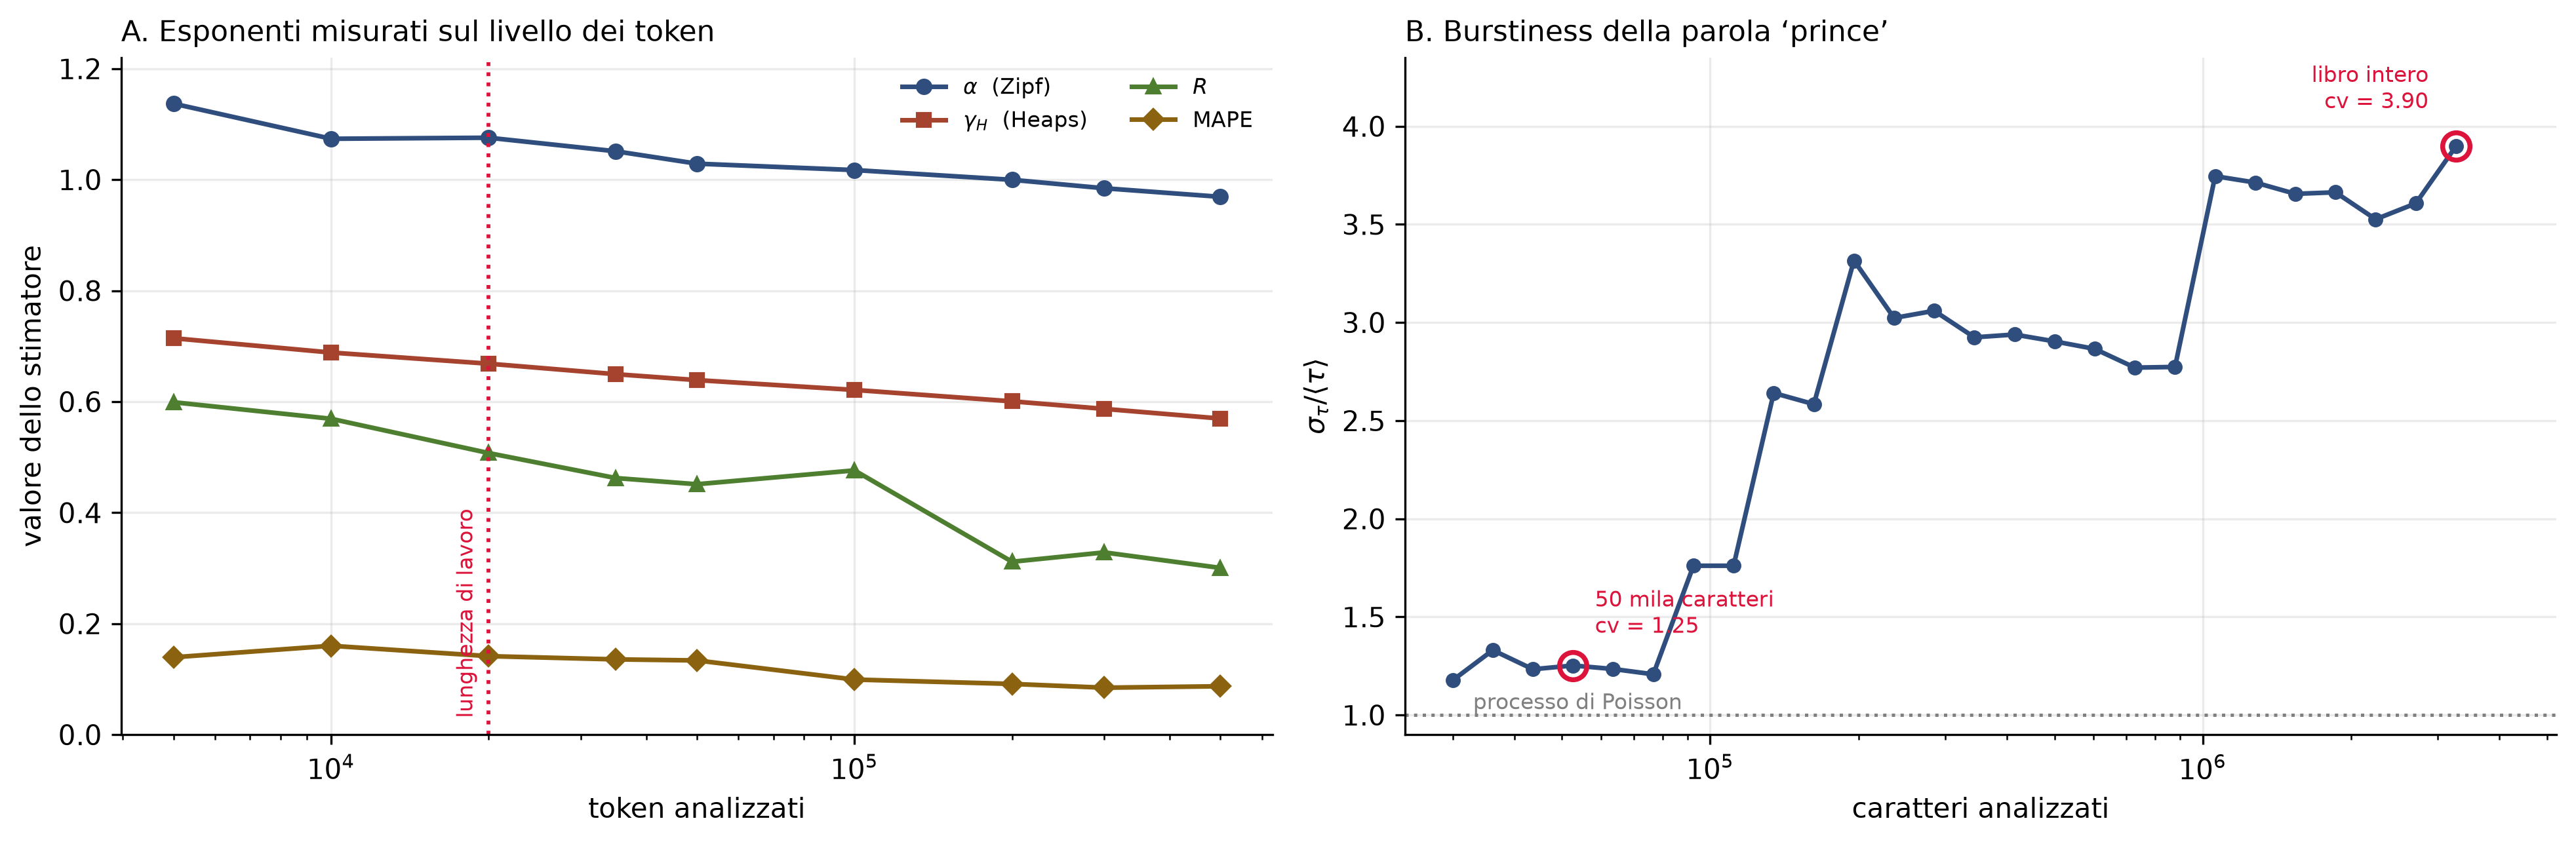
\includegraphics[width=\textwidth]{figure/cap3_dimensione_finita.png}
  \caption{Deriva degli stimatori con la lunghezza di analisi, misurata sulla
  continuazione di \emph{Guerra e pace} usata come baseline umana.
  \textbf{A}: gli esponenti misurati sul livello dei token decrescono tutti in
  modo monotono. Fra \num{5000} e \num{500000} token il descrittore $R$ passa da
  $0.60$ a $0.30$, dimezzandosi, mentre $\gamma_H$ scende da $0.72$ a $0.57$ e
  l'esponente di Zipf da $1.14$ a $0.97$. La linea verticale segna la lunghezza
  di lavoro adottata nei capitoli sperimentali.
  \textbf{B}: il coefficiente di variazione degli intervalli fra occorrenze
  della parola \emph{prince} cresce da $1.25$ su \num{50000} caratteri a $3.90$
  sul romanzo intero. La deriva è quella attesa quando la coda non
  presenta un taglio dentro la finestra osservata: finestre più lunghe
  campionano vuoti più lunghi, e la stima di $\sigma_\tau$ non raggiunge un
  valore limite. Il §\ref{sec:coda-risultati} misura direttamente il taglio e lo
  trova crescere con la finestra, da $13.5$ a $94.7$ intervalli medi fra
  \num{30000} e \num{480000} caratteri: i momenti sono finiti a ogni lunghezza,
  ma il loro valore dipende da essa.
  La Figura~\ref{fig:heaps-finito} mostrava lo stesso fenomeno su un solo
  stimatore ma su tre opere diverse, stabilendone l'universalità; qui il
  confronto è ristretto a un'unica opera e serve invece a quantificare l'entità
  dell'effetto sulla baseline effettivamente impiegata.}
  \label{fig:dimensione-finita}
\end{figure}

L'entità della deriva rende obbligatorie tre precauzioni operative, che valgono
per l'intero lavoro. Tutti i confronti fra corpora vengono condotti alla stessa
lunghezza di analisi, indicata d'ora in avanti con $N_{\mathrm{eff}}$ e
dichiarata per ciascuna fase, poiché non tutte le analisi condividono gli stessi
corpora. Nessun valore assoluto viene confrontato con valori pubblicati misurati
su lunghezze diverse. E ogni riferimento umano viene misurato con le stesse
procedure e alla stessa lunghezza dei testi con cui viene confrontato, anziché
ripreso dalla letteratura: è il paragrafo che segue. Il pannello B mostra il caso
concreto in cui la prima e la seconda precauzione si incontrano, cioè perché il
confronto con il valore pubblicato per \emph{prince} vada condotto sul romanzo
intero e non sui segmenti: è la stessa quantità, misurata su finestre che
differiscono di un fattore sessanta.

Per l'analisi appaiata dei corpora enciclopedici $N_{\mathrm{eff}}$ è fissato a
\num{60000} caratteri. Il valore è il massimo compatibile con la conservazione
di tutte le 39 terne: portandolo a \num{80000} quattro articoli non
raggiungono la soglia e le terne disponibili scendono da 39 a 35. L'intera
catena viene comunque ripetuta a quella lunghezza maggiore come controllo di
robustezza, il cui esito è riportato nel §\ref{sec:robustezza-neff} e distingue
le parti del divario che resistono al cambio di finestra da quelle che non vi
resistono.

Le altre fasi dell'analisi impiegano lunghezze diverse, perché non condividono i
corpora e non sono confrontate fra loro. La Tabella~\ref{tab:fasi} le riassume:
ciascun valore numerico che comparirà nei capitoli sperimentali è riconducibile
a una di queste righe.

\begin{table}[htbp]
\centering
\small
\begin{tabular}{@{}>{\raggedright\arraybackslash}p{2.9cm}>{\raggedright\arraybackslash}p{4.3cm}rll@{}}
\toprule
Fase & Scopo & $N_{\mathrm{eff}}$ & Unità & Analizzate \\
\midrule
Sweep di temperatura & misure sul corpus generato
  & \num{20000} & token & 242 documenti \\
\addlinespace
Raccolta & appaiamento per titolo e verifica di paternità
  & \num{80000} & caratteri & 40 coppie \\
\addlinespace
Fattibilità & verificare che l'effetto esista in prosa enciclopedica, senza
  Grokipedia & \num{50000} & caratteri & 40 voci, 20 segmenti \\
\addlinespace
Analisi principale & confronto appaiato fra i quattro corpora
  & \num{60000} & caratteri & 39 terne \\
\addlinespace
Robustezza & ripetizione dell'intera catena a lunghezza maggiore
  & \num{80000} & caratteri & 35 terne \\
\bottomrule
\end{tabular}
\caption{Le fasi dell'analisi e le rispettive lunghezze. I valori differiscono
perché le fasi non condividono i corpora, e la prima riga adotta una unità
diversa dalle altre per la ragione discussa nel §\ref{sec:unita}. Nessun
confronto attraversa righe diverse della tabella: la fase di fattibilità non
include Grokipedia, e quella sullo sweep non include alcun corpus
enciclopedico.}
\label{tab:fasi}
\end{table}

\paragraph{Baseline umana misurata, non citata.}
Per la stessa ragione, il riferimento umano non viene ripreso dalla letteratura
ma misurato con le stesse procedure e alla stessa lunghezza dei testi generati.
Il testo di riferimento è la continuazione del passaggio usato come prompt: il
confronto è quindi fra continuazione umana e continuazione generata, a parità di
contesto. La Tabella~\ref{tab:baseline} riporta i valori così ottenuti.

\begin{table}[htbp]
\centering
\small
\begin{tabular}{@{}lrr@{}}
\toprule
Grandezza & Misurata qui & Pubblicata \\
\midrule
$\alpha$ (Zipf)                 & 1.076  & $1.006 \pm 0.05$ \\
MAPE                            & 0.141  & $0.156 \pm 0.077$ \\
$\gamma_H$ (Heaps)              & 0.668  & $0.801 \pm 0.02$ \\
$R$                             & 0.507  & $0.17 \pm 0.05$ \\
$\alpha_{\mathrm{DFA}}$         & 0.579  & --- \\
$R_{\mathrm{gzip}}$             & 0.381  & --- \\
entropia [bit/carattere]        & 2.227  & --- \\
\bottomrule
\end{tabular}
\caption{Baseline umana misurata su \num{20000} token di \emph{Guerra e pace},
confrontata con i valori pubblicati in~\cite{mikhaylovskiy2025zipf}. Questi
ultimi sono calcolati su opere intere e non costituiscono un riferimento valido
per testi di questa lunghezza, per la ragione discussa nel
§\ref{sec:validazione}.}
\label{tab:baseline}
\end{table}

\paragraph{Appaiamento in frequenza dei controlli.}
Nel confronto fra parole di contenuto e parole di controllo, ciascun sostantivo
viene appaiato alla parola non-sostantivo di frequenza più vicina, minimizzando
$\lvert\log(f_w/f_k)\rvert$. L'appaiamento è indispensabile perché la burstiness
dipende dalla frequenza: confrontare parole di frequenza diversa misurerebbe
quella differenza anziché la natura semantica delle parole.

\paragraph{Selezione dei bersagli entro ciascun testo.}
Le parole bersaglio vengono scelte all'interno di ogni documento anziché fissate
una volta per tutte sul corpus di riferimento. La scelta è necessaria perché
corpora diversi trattano argomenti diversi e non condividono il lessico
tematico, ed è inoltre più efficiente, poiché produce un numero maggiore di
confronti appaiati a parità di corpus.

\paragraph{Come vengono separati i livelli lessicali.}
\label{par:livelli-lessicali}
Dentro ciascun documento le parole vengono ordinate per frequenza e ripartite in
tre insiemi. Le \emph{parole funzione} sono le sei più frequenti fra quelle che
compaiono in una lista chiusa di funtori inglesi. Le \emph{parole chiave} sono
le sette più frequenti fra quelle che superano i quattro caratteri e non
figurano in quella lista, oppure che risultano nomi propri per il criterio di
maiuscola in posizione interna alla frase descritto sopra. I \emph{controlli
appaiati} sono, per ciascuna parola chiave, la parola di frequenza più vicina
fra quelle rimaste. La ripartizione è dunque interamente determinata dalla lista
dei funtori, e la sua completezza è una scelta di metodo con conseguenze
misurabili.

La lista impiegata inizialmente conteneva \num{133} voci e ometteva alcuni
connettivi e attenuatori inglesi molto comuni, fra cui \emph{like},
\emph{amid}, \emph{including}, \emph{though}, \emph{also}, \emph{rather} e
\emph{without}. In un corpus in cui quei termini restano rari l'omissione è
innocua; in Grokipedia non lo è, perché il testo generato li impiega molto più
spesso: \emph{like} entrava fra le sette parole più frequenti in \num{29} voci
su \num{39}, contro nessuna di Wikipedia. Finivano quindi classificati come
parole chiave. Poiché i connettivi ricorrono a cadenza quasi costante e hanno
perciò burstiness bassa, il livello lessicale alto di Grokipedia risultava
contaminato da materiale che appartiene al livello dei funtori, e il divario
misurato a quel livello ne usciva gonfiato.

La lista è stata quindi estesa a \num{215} voci per classe grammaticale, cioè
preposizioni, congiunzioni subordinanti, avverbi connettivi e attenuatori e
quantificatori, e applicata identica a tutti e quattro i corpora. L'estensione
non rimuove nulla: le parole interessate passano al livello dei funtori, e al
loro posto sale fra le parole chiave la parola di contenuto successiva in
ordine di frequenza, cosicché tutti i livelli conservano la stessa numerosità
in tutti i corpora. Tutte le misure del Capitolo~\ref{cap:risultati2} sono
calcolate con la lista estesa; il §\ref{sec:effetto-stoplist} riporta di
quanto si spostano i risultati, perché lo spostamento non è trascurabile e la
scelta va resa verificabile.

% ---------------------------------------------------------------------
\section{Validazione delle procedure di calcolo}
\label{sec:validazione}

Ogni conclusione di questo lavoro poggia sul fatto che il codice misuri
effettivamente le quantità definite nel Capitolo~\ref{cap:teoria}. La
validazione procede per due vie indipendenti: la riproduzione di valori
pubblicati e la misura di grandezze il cui valore esatto è noto per costruzione.

\paragraph{Riproduzione di valori pubblicati.}
Le quantità del protocollo di Altmann sono state misurate sul corpus letterario
e confrontate con quelle riportate in~\cite{altmann2012}. Il null model A1, che
per costruzione deve restituire $\hat\gamma_{A1} \simeq 1$, dà valori compresi
fra $0.972$ e $0.984$ ai quattro livelli linguistici esaminati.

La seconda quantità riprodotta è il coefficiente di variazione della parola
\emph{prince}, che vale $3.89$ sul libro intero, in accordo con il $3.86$
pubblicato, ma scende a $1.30$ sui segmenti da \num{50000} caratteri impiegati
nei confronti. Non si tratta di un disaccordo: è la deriva di dimensione finita del
§\ref{sec:lunghezza}, e mostra perché i valori assoluti non vadano confrontati
fra lunghezze diverse. Il confronto con il valore pubblicato è quindi condotto
sul libro intero, mentre i confronti fra corpora usano la lunghezza comune.

\paragraph{Misura di esponenti noti.}
La seconda via non dipende da alcuna pubblicazione. Le procedure sono state
applicate a segnali costruiti in modo che il risultato atteso sia noto
analiticamente, ottenendo i valori della Tabella~\ref{tab:validazione}.

\begin{table}[htbp]
\centering
\small
\begin{tabular}{@{}l>{\raggedright\arraybackslash}p{5.6cm}rr@{}}
\toprule
Procedura & Segnale di prova & Atteso & Ottenuto \\
\midrule
DFA & rumore bianco & 0.500 & 0.510 \\
DFA & cammino aleatorio & 1.500 & 1.494 \\
Stimatore KL & testo confrontato con sé stesso & 0 & $0$ esatto \\
Stimatore KL & due campioni della stessa sorgente & $\simeq 0$ & 0.001 \\
Stimatore KL & sorgenti diverse & $> 0$ & 0.687 \\
\bottomrule
\end{tabular}
\caption{Validazione su segnali a esponente noto. Le prime due righe verificano
l'esponente della detrended fluctuation analysis; le ultime tre verificano che
lo stimatore della divergenza di Kullback--Leibler si annulli esattamente sul
confronto di un testo con sé stesso, resti prossimo a zero fra campioni della
stessa sorgente e cresca fra sorgenti diverse.}
\label{tab:validazione}
\end{table}

La proprietà $D(x\|x) = 0$ non è un accordo approssimato ma un'identità esatta,
e costituisce il controllo più stringente sullo stimatore della divergenza:
come discusso nel §\ref{sec:crossparsing}, essa vale soltanto se i riferimenti
usati nei due termini hanno la stessa lunghezza, e una sua violazione
segnalerebbe immediatamente l'errore.

% ---------------------------------------------------------------------
\section{Controlli di robustezza}
\label{sec:robustezza}

I controlli di questa sezione non verificano che le procedure siano corrette, ma
che i risultati non dipendano da scelte che avrebbero potuto essere compiute
diversamente.

\paragraph{Ordine del detrending.}
La detrended fluctuation analysis rimuove dalle finestre le tendenze polinomiali
fino a un grado fissato. L'intera analisi è stata condotta con il grado 1 e con
il grado 2, e la Tabella~\ref{tab:ordine-dfa} riporta le due stime a ciascuna
temperatura. Le misure riportate nel Capitolo~\ref{cap:risultati1} usano il
grado 2, per la ragione che il confronto stesso rende evidente: dove il segnale
è stazionario i due gradi coincidono, e dove non lo è il grado 1 restituisce un
esponente sistematicamente più alto, perché lascia nel segnale una tendenza che
non è correlazione.

\begin{table}[htbp]
\centering
\small
\begin{tabular}{@{}lrrrrr@{}}
\toprule
$T$ & grado 1 & grado 2 & scarto & dispersione & documenti \\
\midrule
0.4 & 0.284 & 0.307 & $-0.046$ & 0.085 & 21 \\
0.5 & 0.582 & 0.500 & $-0.132$ & 0.081 & 21 \\
0.6 & 0.613 & 0.416 & $-0.124$ & 0.093 & 21 \\
0.7 & 0.713 & 0.583 & $-0.115$ & 0.073 & 21 \\
0.8 & 0.715 & 0.601 & $-0.138$ & 0.070 & 20 \\
0.9 & 0.758 & 0.659 & $-0.078$ & 0.050 & 18 \\
1.0 & 0.753 & 0.711 & $-0.014$ & 0.054 & 17 \\
1.1 & 0.651 & 0.564 & $-0.060$ & 0.046 & 19 \\
1.2 & 0.570 & 0.556 & $-0.029$ & 0.035 & 21 \\
1.3 & 0.563 & 0.535 & $-0.007$ & 0.024 & 21 \\
1.4 & 0.535 & 0.532 & $-0.009$ & 0.019 & 21 \\
1.5 & 0.529 & 0.527 & $-0.006$ & 0.015 & 21 \\
\midrule
\multicolumn{3}{@{}l}{testo umano} & $-0.007$ & --- & 1 \\
\bottomrule
\end{tabular}
\caption{Esponente della fluttuazione stimato con detrending di grado 1 e di
grado 2. Le prime tre colonne numeriche riportano mediane sui documenti
disponibili a ciascuna temperatura; la quarta è la deviazione standard dello
scarto fra i due gradi, calcolata documento per documento. Lo scarto è negativo
ovunque, come atteso, perché il grado 2 rimuove tendenze che il grado 1 lascia
nel segnale.}
\label{tab:ordine-dfa}
\end{table}

Le due stime coincidono dove il segnale è stazionario. Sulla baseline umana lo
scarto vale $-0.007$, e sui testi generati da $T = 1.2$ in su la sua mediana vale
$-0.010$ a fronte di una dispersione fra documenti di $0.027$: la differenza fra
i due gradi è più piccola della variabilità fra documenti generati nelle stesse
condizioni, e l'esponente non dipende in modo apprezzabile dalla scelta del
detrending.

Nell'intervallo $T \in [0.5, 0.8]$ lo scarto mediano vale invece $-0.125$, con
dispersione $0.078$: qui la differenza supera nettamente la variabilità ed è
quindi reale. È concentrata nel regime in cui il testo degenera in cicli di
ripetizione e la serie dei ranghi non è stazionaria, e in quel regime,
coerentemente con quanto osservato nel §\ref{sec:ponte}, l'esponente va letto
come indicatore di periodicità e non come misura di correlazione a lungo raggio.


\paragraph{Numerosità disuguale fra celle.}
Dalla disuguale numerosità dichiarata nel §\ref{sec:protocollo} discendono due
limitazioni. Per il modello da 14 miliardi di parametri non esiste una stima
della dispersione fra campioni, cosicché nelle sue figure le barre d'errore non
sono definite e ogni suo valore è una singola realizzazione; e le deviazioni
standard riportate nelle figure del Capitolo~\ref{cap:risultati1} non sono
confrontabili fra modelli, poiché derivano da un numero diverso di campioni. Le
conclusioni che riguardano il confronto fra modelli vanno lette con questa
avvertenza, che il §\ref{sec:zipf-risultati} riprende quantitativamente sul
caso in cui pesa di più.

% ---------------------------------------------------------------------
\section{Riproducibilità}
\label{sec:riproducibilita}

Tutte le procedure sono deterministiche a semi fissati, e i semi impiegati sono
registrati nel codice. I corpora scaricati da fonti esterne sono conservati in
copia locale, così che una modifica successiva della fonte non alteri i
risultati: vale in particolare per le voci di Grokipedia, che vengono riscritte
senza cronologia pubblica.

I dati intermedi e le figure sono prodotti da notebook che salvano ogni risultato
in file separati, in formato aperto, insieme a una sintesi testuale dei
parametri usati e delle scelte compiute, così che ciascuna figura sia
ricostruibile senza ripetere i calcoli.


% =====================================================================
%  Capitolo 4 — Il testo generato lungo lo sweep di temperatura
%  Incluso da main.tex con % =====================================================================
%  Capitolo 4 — Il testo generato lungo lo sweep di temperatura
%  Incluso da main.tex con % =====================================================================
%  Capitolo 4 — Il testo generato lungo lo sweep di temperatura
%  Incluso da main.tex con \input{capitolo4_sweep_temperatura}
%  Figure del corpo: modello Qwen2.5-3B. Quelle degli altri quattro
%  modelli stanno nel repository indicato in Appendice A.
% =====================================================================

\chapter{Il testo generato lungo lo sweep di temperatura}
\label{cap:risultati1}

Questo capitolo applica ai \num{242} documenti generati le misure introdotte nel
Capitolo~\ref{cap:teoria}, facendo variare la sola temperatura di campionamento.
Ogni misura viene confrontata con la baseline umana della
Tabella~\ref{tab:baseline}, calcolata con le stesse procedure e alla stessa
lunghezza.

Le figure del corpo del capitolo mostrano il modello Qwen2.5-3B, scelto come
esemplare perché dispone di cinque campioni per quasi tutte le temperature e
presenta le curve meno rumorose; le corrispondenti figure per gli altri quattro
modelli sono depositate nel repository indicato
nell'Appendice~\ref{app:codice}. Le curve aggregate
riportano invece tutti e cinque i modelli.

Il risultato principale non è nessuna delle singole misure, ma il fatto che
convergano: criteri tratti da quattro lavori indipendenti, costruiti per scopi
diversi, individuano la stessa regione di temperature. Il §\ref{sec:tstar} lo
documenta.

% ---------------------------------------------------------------------
\section{Le tre modalità di fallimento}
\label{sec:fallimenti}

La prima e la terza riga della Tabella~\ref{tab:tre-regimi} sono entrambe
prodotte dai modelli qui analizzati, a due temperature diverse, e mostrano i
due modi in cui la generazione si allontana dal linguaggio: la ripetizione letterale a bassa
temperatura, l'incoerenza semantica ad alta temperatura. Salendo ancora si
incontra un terzo regime, in cui l'alfabeto stesso si disgrega e il testo diventa
un miscuglio di sistemi di scrittura diversi.

Le tre modalità possono essere separate quantitativamente. Un documento viene
classificato come degenerato per \emph{ripetizione} se la quota di 8-grammi
ripetuti supera $0.10$, contro il valore $0.000$ misurato sul testo umano; come
degenerato nell'\emph{alfabeto} se la quota di caratteri non ASCII supera
$0.05$, più del triplo del valore umano $0.014$; come degenerato nel
\emph{lessico} se meno del $70\%$ delle sue parole possiede un vettore nello
spazio di embedding, contro il $98\%$ del testo umano. Le tre condizioni non si
escludono a vicenda, e un documento può soddisfarne più di una.

La Tabella~\ref{tab:fallimenti} riporta i conteggi.

\begin{table}[htbp]
\centering
\small
\begin{tabular}{@{}l>{\raggedright\arraybackslash}p{5.4cm}rr@{}}
\toprule
Modalità & Criterio & Documenti & Quota \\
\midrule
Ripetizione & 8-grammi ripetuti $> 0.10$      & 122 & 50\,\% \\
Alfabeto    & caratteri non ASCII $> 0.05$    & 125 & 52\,\% \\
Lessico     & copertura degli embedding $< 0.70$ & 112 & 46\,\% \\
\midrule
Nessuna     & prosa inglese non degenerata    &   2 &  1\,\% \\
\bottomrule
\end{tabular}
\caption{Modalità di degenerazione dei \num{242} documenti generati. Le
categorie non sono disgiunte. La classificazione dipende dalle soglie scelte,
ma non nella sostanza: facendole variare entro intervalli ragionevoli il numero
di documenti non degenerati resta compreso fra 2 e 7, cioè fra l'uno e il tre
per cento del totale.}
\label{tab:fallimenti}
\end{table}

Il dato va letto con attenzione, perché è il presupposto dell'intera seconda
parte sperimentale. Non significa che i modelli siano incapaci di produrre
linguaggio, ma che la finestra di temperature in cui lo producono è
sufficientemente stretta da non essere coperta da uno sweep a passo $0.1$: i
soli due documenti non degenerati compaiono a $T = 1.0$, e già a $T = 0.9$ e
$T = 1.1$ tutti i campioni ricadono in almeno una delle tre categorie. Il
Capitolo~\ref{cap:risultati2} muove da questa constatazione.


% ---------------------------------------------------------------------
\section{Legge di Zipf}
\label{sec:zipf-risultati}

La Figura~\ref{fig:zipf-cum} riporta gli istogrammi cumulativi delle frequenze,
una curva per temperatura, con la curva umana per confronto.

\begin{figure}[htbp]
  \centering
  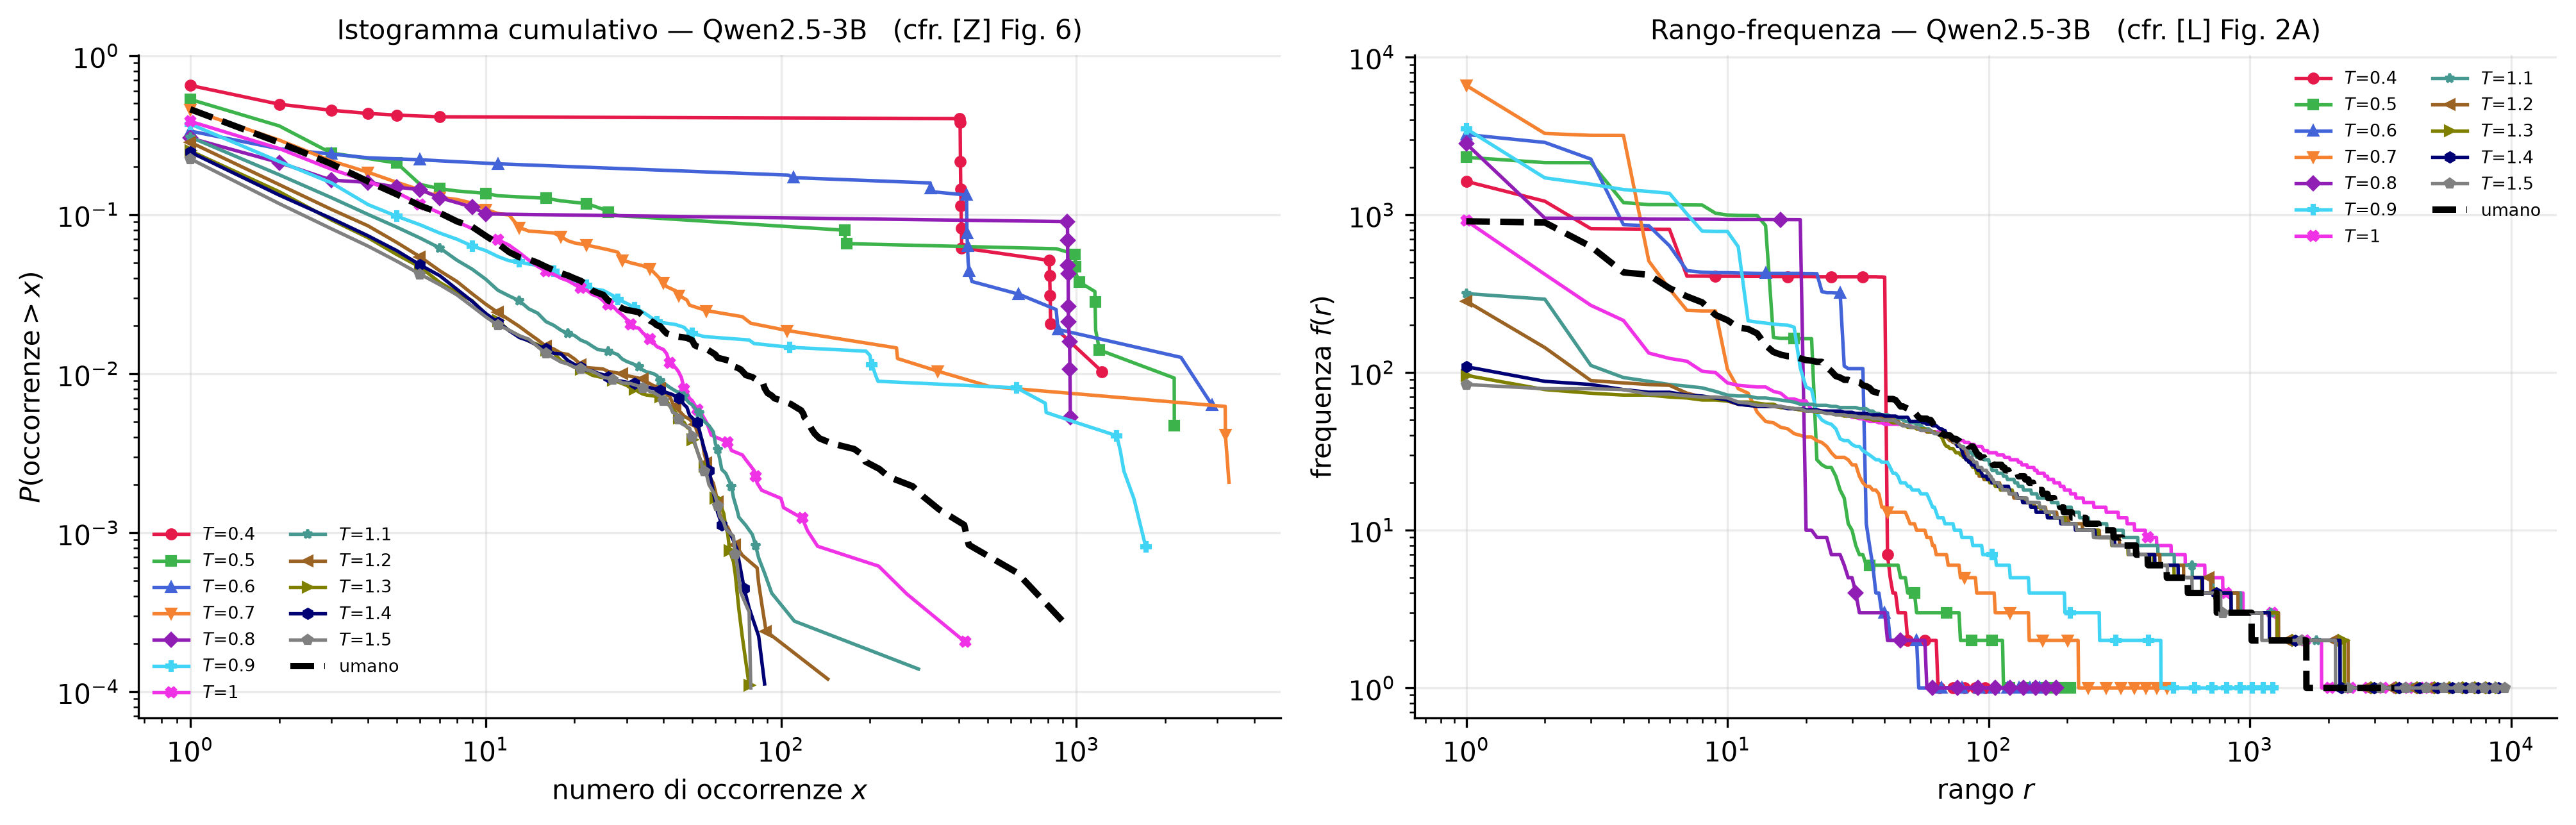
\includegraphics[width=\textwidth]{figure/cap4_zipf_cumulativo_Qwen25_3B.png}
  \caption{Istogrammi cumulativi delle frequenze dei token per il modello
  Qwen2.5-3B, una curva per temperatura. A bassa temperatura la curva è quasi
  verticale, perché pochi token coprono l'intero documento; ad alta temperatura
  è quasi orizzontale, perché quasi ogni token compare una volta sola. Solo
  nella regione intermedia la curva si avvicina alla retta che in coordinate
  bilogaritmiche corrisponde a una legge di potenza.}
  \label{fig:zipf-cum}
\end{figure}

L'esponente da solo non basta a descrivere questo comportamento, ed è la ragione
per cui nel §\ref{sec:zipf} è stato introdotto il MAPE: una curva può avere la
pendenza corretta e una curvatura marcata, e in tal caso l'esponente stimato non
descrive nulla. La Figura~\ref{fig:zipf-vs-T} riporta entrambe le quantità in
funzione della temperatura.

\begin{figure}[htbp]
  \centering
  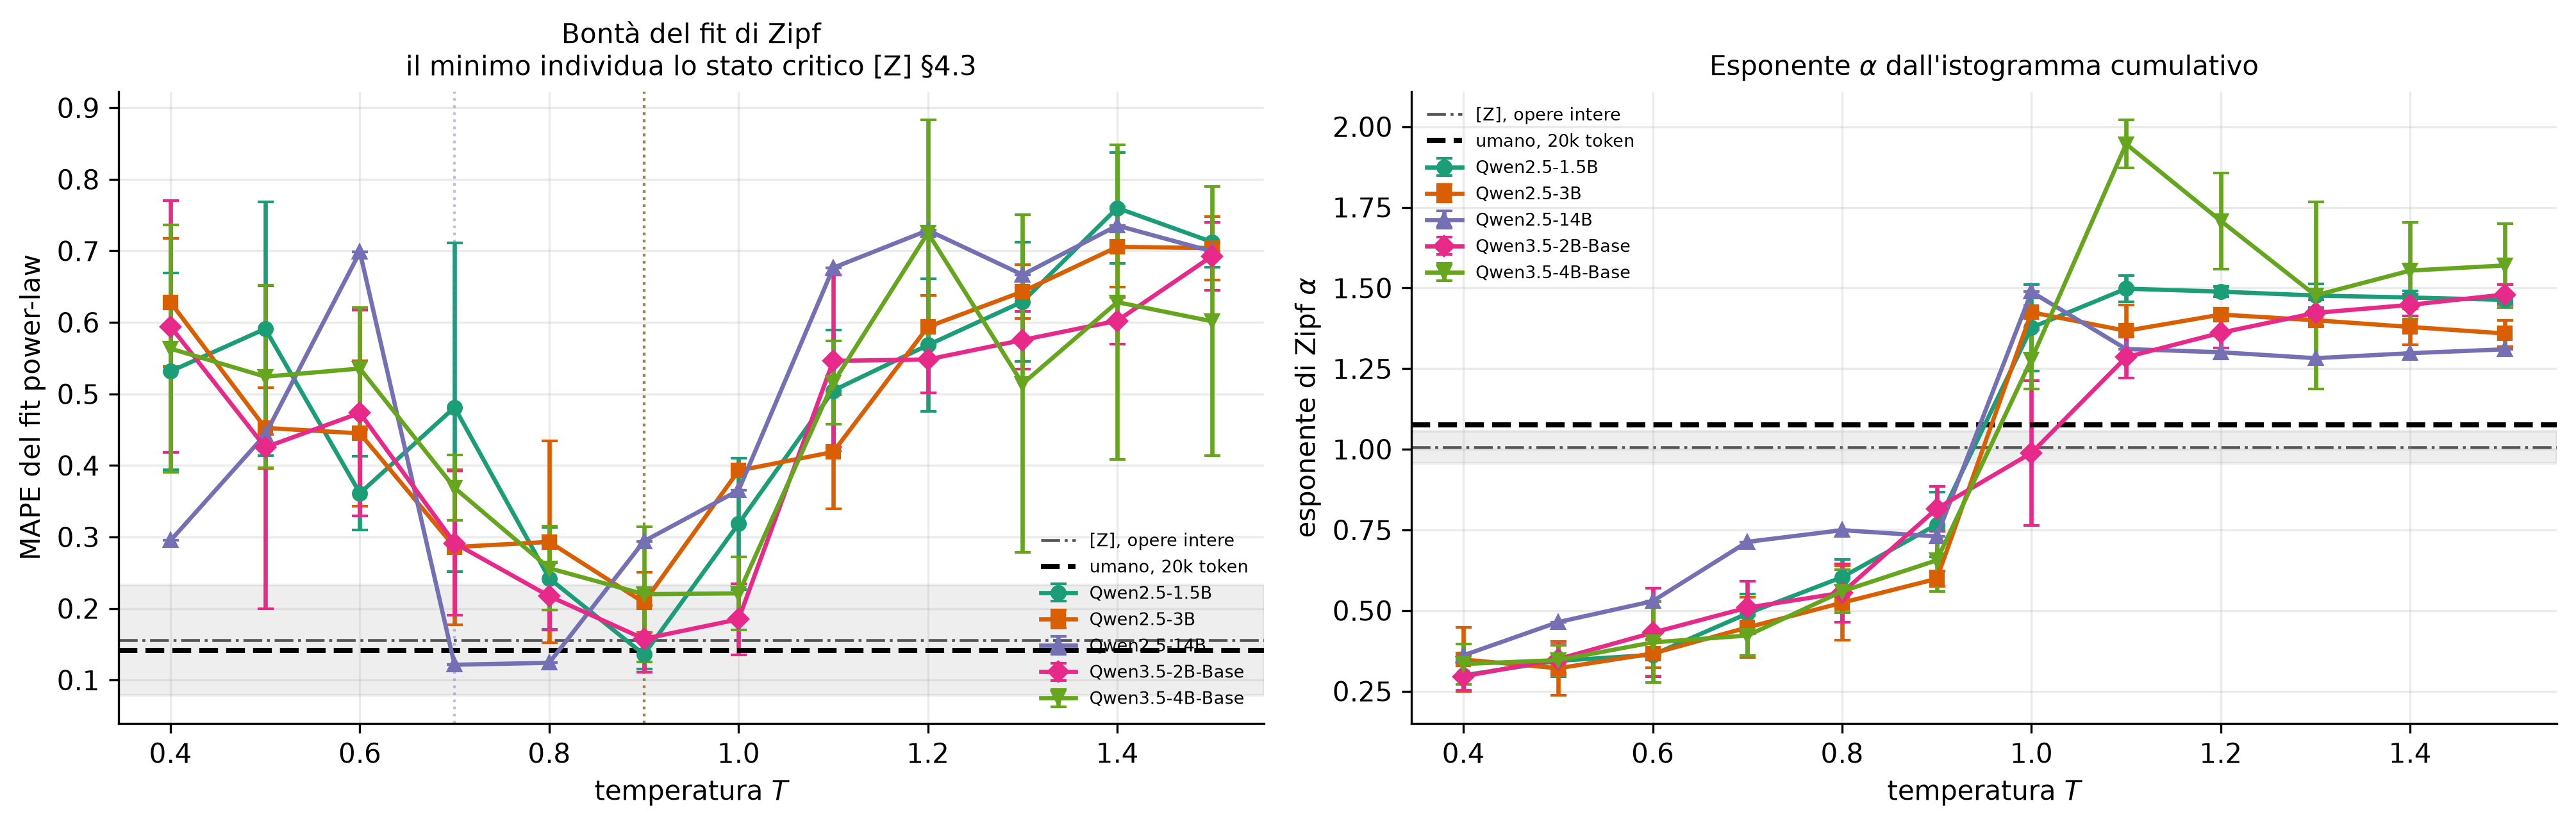
\includegraphics[width=\textwidth]{figure/cap4_zipf_vs_T.png}
  \caption{Bontà del fit e esponente della legge di Zipf in funzione della
  temperatura, per tutti e cinque i modelli. La banda grigia è il valore
  pubblicato su testi letterari interi, la linea nera tratteggiata la baseline
  umana misurata alla lunghezza di lavoro.}
  \label{fig:zipf-vs-T}
\end{figure}

Il MAPE ha un minimo pronunciato, che cade a $T = 0.9$ per quattro modelli su
cinque e a $T = 0.7$ per il modello da 14 miliardi di parametri. È il
risultato centrale della sezione: esiste una temperatura alla quale la
distribuzione delle frequenze del testo generato è più vicina a una legge di
potenza, e ai due lati di essa l'aderenza peggiora rapidamente.

Al minimo il MAPE del modello esemplare vale $0.208$. I due termini di
riferimento sono la baseline umana misurata alla stessa lunghezza, che vale
$0.141$, e il valore $0.156 \pm 0.077$ che~\cite{mikhaylovskiy2025zipf} riporta
su un corpus di sei opere letterarie in cinque lingue. Che i due riferimenti
umani cadano tanto vicini è una verifica indipendente della taratura della
baseline: sono ottenuti con tokenizzatori diversi, su testi diversi e di
lunghezza diversa, e la deriva documentata nella
Figura~\ref{fig:dimensione-finita} non rendeva scontato l'accordo.

Il valore del modello va letto contro tre metri diversi, e il giudizio che se ne
ricava non è lo stesso. Rispetto al modello stesso, $0.208$ è un risultato
netto: alle due estremità dell'intervallo lo stesso modello dà $0.628$ e
$0.704$, cioè un errore di fit tre volte più grande. Rispetto al testo umano è
invece una mezza vittoria: $0.208$ è circa una volta e mezza $0.141$, e resta
dentro la banda pubblicata solo perché quella banda è larga, sfiorandone il
margine superiore $0.233$. Rispetto agli altri modelli, infine, è un risultato
mediocre. La Tabella~\ref{tab:mape-minimi} riporta i cinque minimi: due modelli
scendono sotto il valore umano e un terzo vi si accosta, con $0.158$ contro
$0.141$, mentre il modello esemplare e il Qwen3.5-4B restano sopra.

\begin{table}[htbp]
\centering
\small
\begin{tabular}{@{}lrr@{}}
\toprule
Modello & $T$ del minimo & MAPE al minimo \\
\midrule
Qwen2.5-14B      & 0.7 & 0.121 \\
Qwen2.5-1.5B     & 0.9 & 0.136 \\
Qwen3.5-2B-Base  & 0.9 & 0.158 \\
Qwen2.5-3B       & 0.9 & 0.208 \\
Qwen3.5-4B-Base  & 0.9 & 0.220 \\
\midrule
testo umano      & --- & 0.141 \\
\bottomrule
\end{tabular}
\caption{Valore minimo del MAPE e temperatura alla quale viene raggiunto, per
ciascun modello, con la baseline umana misurata alla stessa lunghezza. Il
minimo esiste per tutti e cinque, ma solo tre modelli lo portano al livello del
testo umano o sotto. La riga del Qwen2.5-14B è ricavata da un solo campione per
temperatura e va letta con la cautela discussa nel testo.}
\label{tab:mape-minimi}
\end{table}

La prima riga della tabella richiede una precauzione. Il Qwen2.5-14B è l'unico
modello con un solo campione per temperatura, contro i tre o cinque degli altri,
e la sua curva del MAPE non è regolare da nessuno dei due lati del minimo: vale
$0.295$ a $T = 0.4$, sale a $0.698$ a $T = 0.6$ e scende a $0.121$ a $T = 0.7$,
cioè peggiora di un fattore due e migliora di un fattore sei in due passi
consecutivi. Negli altri quattro modelli la dispersione fra campioni alla stessa
temperatura va da $0.046$ a $0.230$ attorno a $T = 0.7$, mentre la distanza fra
il minimo del 14B e il suo valore a $T = 0.9$ vale $0.173$: sta dentro
quell'intervallo. Con una sola realizzazione la posizione del minimo non è
risolvibile, e il valore $T = 0.7$ va letto come compatibile con il $T = 0.9$
degli altri quattro anziché come uno spostamento reale. La stessa cautela vale
per la profondità: $0.121$ è il minimo più basso dei cinque ed è anche il meno
affidabile, mentre il $0.136$ del Qwen2.5-1.5B poggia su cinque campioni con
dispersione $0.020$ ed è l'unico caso in cui il primato sul testo umano è
sostenuto da repliche.

La posizione del minimo va confrontata con quella riportata nella fonte.
In~\cite{mikhaylovskiy2025zipf} il minimo del MAPE cade fra $t = 1.0$ e
$t = 1.2$ per tutti i modelli tranne i Llama più grandi, mentre qui cade a
$T = 0.9$ per quattro modelli su cinque. Lo scarto è nella direzione prevista
dall'effetto del prompt descritto nel §\ref{sec:protocollo}, che abbassa
l'errore del fit soprattutto alle basse temperature e sposta quindi il minimo
verso sinistra.

Ne segue una distinzione che vale per tutto il seguito. L'esistenza
di una temperatura ottimale è un fatto generale, comune a tutti e cinque i
modelli; la qualità dell'ottimo, cioè quanto il testo generato in quel punto
somigli davvero a un testo umano, varia da modello a modello e non è garantita.
Il modello scelto come esemplare non è fra quelli che ci riescono, e i grafici
del corpo del capitolo vanno letti tenendolo presente.

L'esponente $\alpha$ racconta la stessa storia da un'altra angolazione. Per il
modello esemplare passa da $0.35$ a $T = 0.4$, valore che corrisponde a una
distribuzione dominata da pochissimi tipi, a $1.36$ a $T = 1.5$, dove più di tre
quarti dei tipi compaiono una volta sola.\footnote{Un tipo che compare una sola
volta nel testo si dice \emph{hapax}. Gli hapax sono normalmente la maggioranza
dei tipi ma una piccola parte delle occorrenze: nella baseline umana usata qui
sono il $54\%$ dei tipi e il $10\%$ dei token, mentre a $T = 1.5$ il modello
esemplare arriva al $77\%$ dei tipi e al $37\%$ dei token.} La transizione non è
graduale: fra $T = 0.9$ e $T = 1.0$ l'esponente salta da $0.60$ a $1.43$,
attraversando in un solo passo il valore umano $1.076$, per poi assestarsi
attorno a $1.4$ senza più avvicinarvisi.

% ---------------------------------------------------------------------
\section{Legge di Heaps e descrittore \texorpdfstring{$R$}{R}}
\label{sec:heaps-risultati}

Le curve di crescita del vocabolario rendono immediatamente evidente perché il
§\ref{sec:heaps} abbia dovuto introdurre un descrittore alternativo all'esponente di
Heaps.

\begin{figure}[htbp]
  \centering
  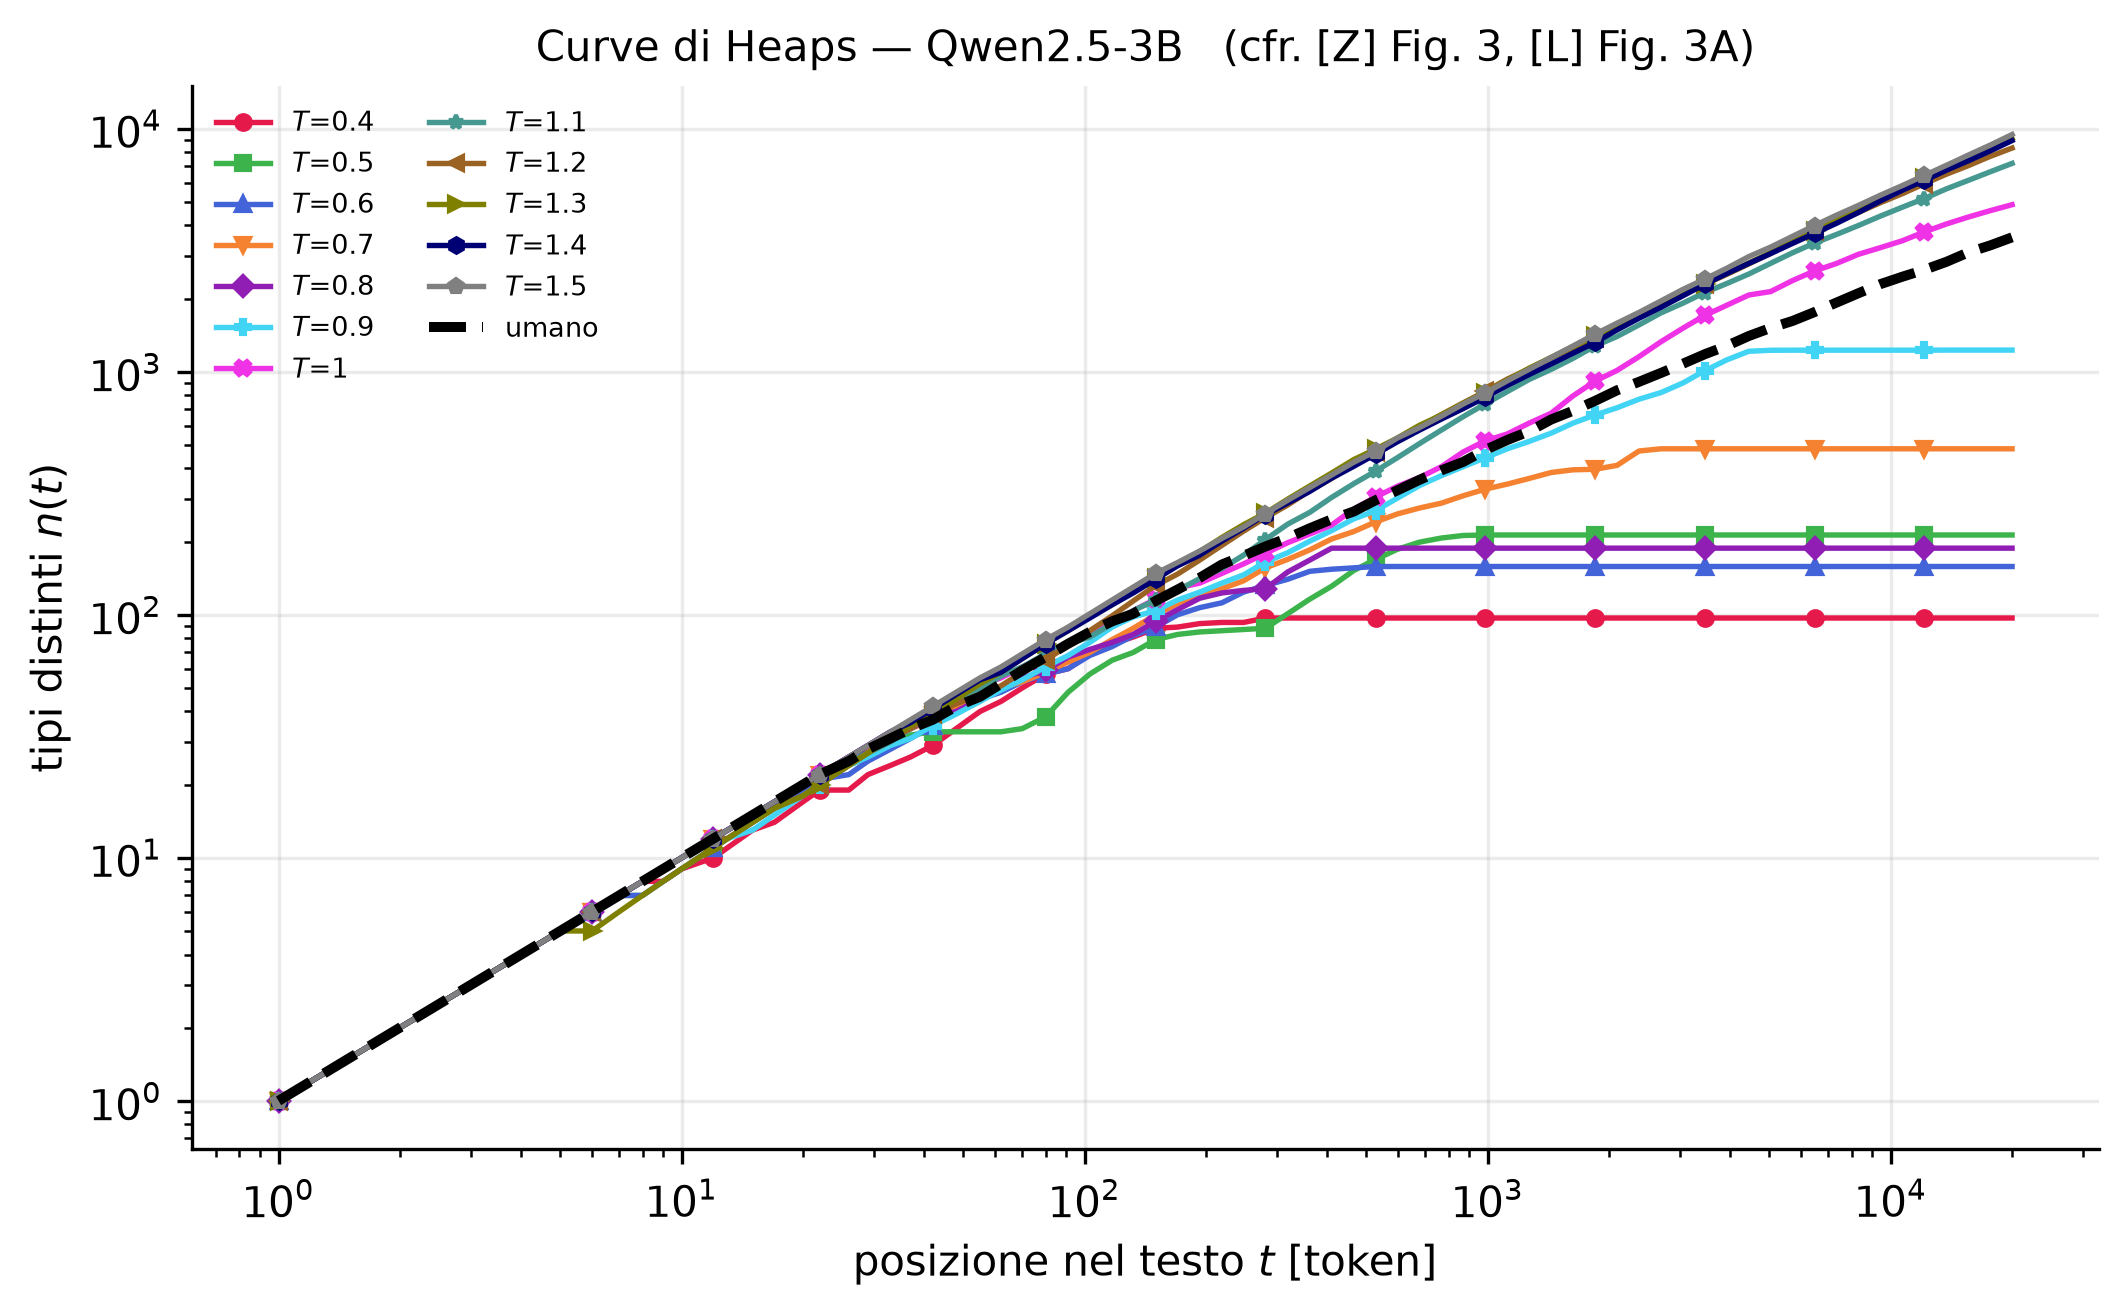
\includegraphics[width=0.86\textwidth]{figure/cap4_heaps_curve_Qwen25_3B.png}
  \caption{Crescita del vocabolario per il modello Qwen2.5-3B. Alle temperature
  basse la curva si appiattisce dopo poche migliaia di token: il modello ha
  smesso di produrre tipi nuovi. Alle temperature alte cresce quasi linearmente.
  In nessuno dei due casi la curva è una legge di potenza, e stimarne
  l'esponente restituisce un numero privo di contenuto.}
  \label{fig:heaps-curve}
\end{figure}

La Figura~\ref{fig:heaps-R} riporta il descrittore $R$, l'esponente $\gamma_H$
e il rapporto fra tipi e occorrenze in funzione della temperatura. I tre
andamenti sono concordi: per il modello esemplare $\gamma_H$ passa da $0.001$
a $T = 0.4$, dove la curva è piatta e il vocabolario non cresce affatto, a
$0.806$ a $T = 1.5$, attraversando il valore umano $0.668$ poco sopra $T =
0.9$. Il descrittore $R$ passa da $0.003$ a $0.688$ e incrocia il valore umano
$0.507$ attorno a $T = 1.05$.

Il terzo pannello riporta la quantità più elementare delle tre, il rapporto fra
il numero di tipi distinti e il numero di occorrenze, e serve da controllo sulle
altre due. A differenza di $\gamma_H$ e di $R$ non richiede alcun fit né alcuna
partizione del documento, quindi non può essere alterato da un modello mal
specificato: se le tre curve concordano, l'andamento non è un artefatto della
procedura di stima. Per il modello esemplare passa da $0.007$ a $T = 0.4$ a
$0.474$ a $T = 1.5$, e attraversa il valore umano $0.179$ fra $T = 0.9$ e
$T = 1.0$, cioè nello stesso punto delle altre due misure. Il pannello mostra
però anche in che senso l'accordo con il testo umano sia solo locale: sopra
$T = 1.1$ il rapporto supera il doppio del valore umano e continua a crescere,
mentre $\gamma_H$ resta stabile attorno a $0.8$. Le due misure smettono di dire
la stessa cosa non appena il vocabolario si allarga oltre quello di un romanzo.

\begin{figure}[htbp]
  \centering
  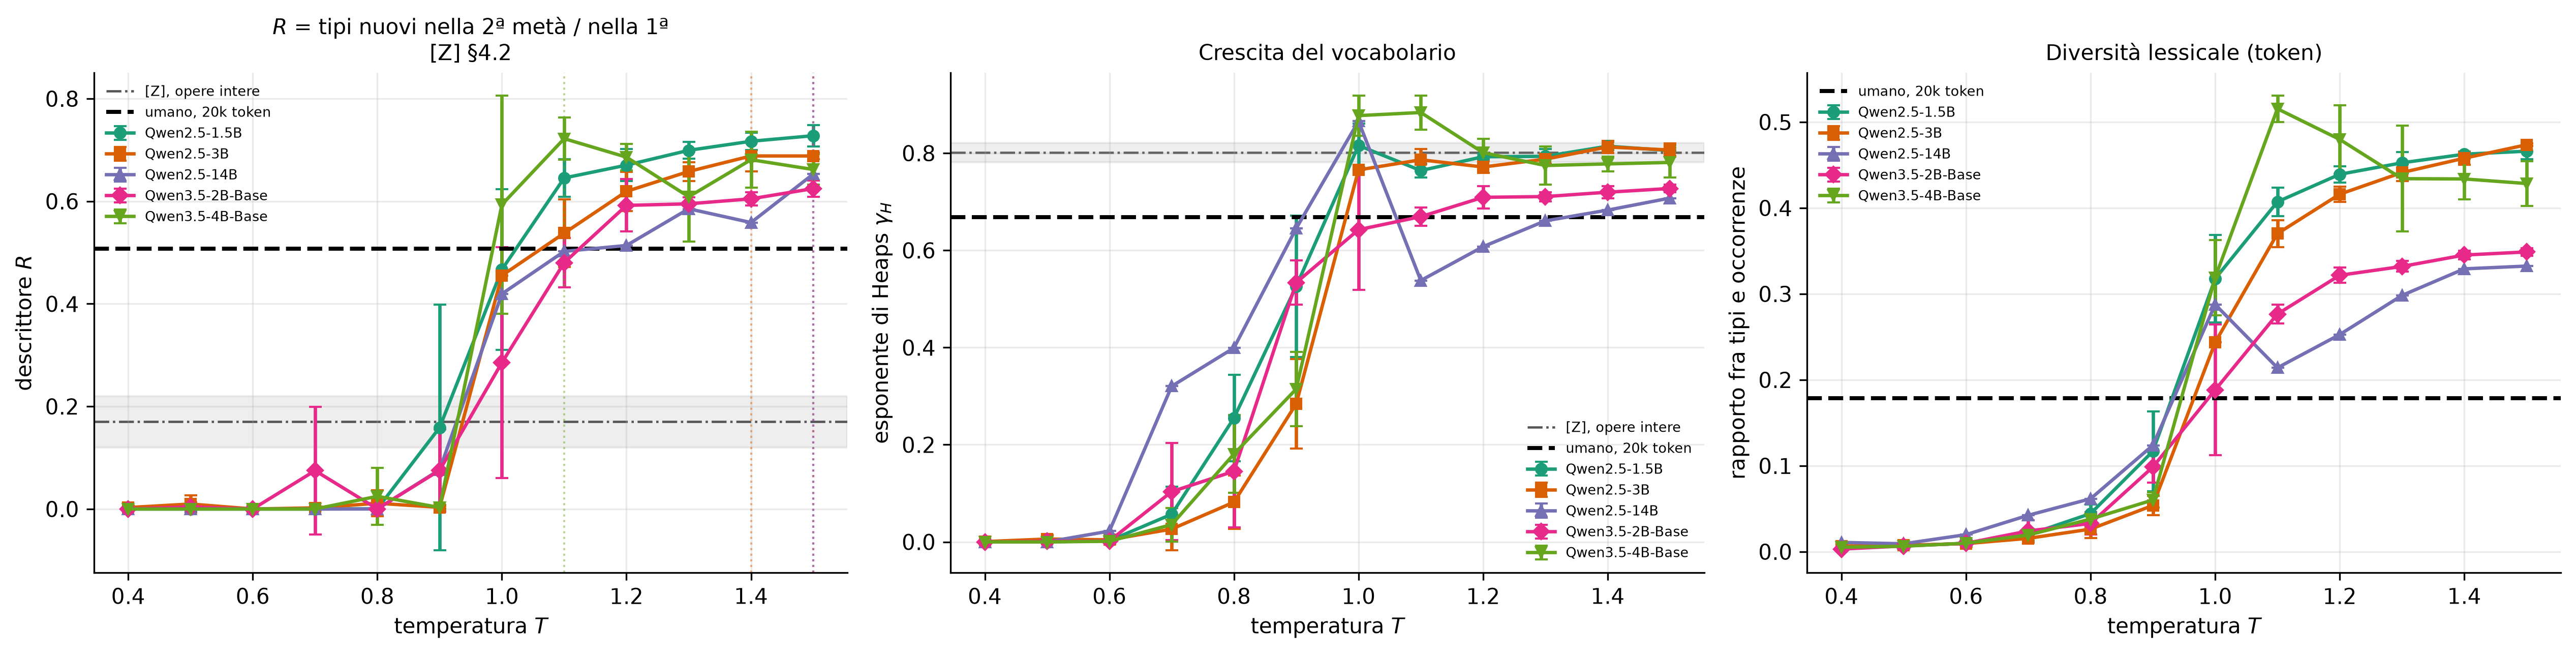
\includegraphics[width=\textwidth]{figure/cap4_heaps_R_vs_T.png}
  \caption{Descrittore $R$, esponente di Heaps e rapporto fra tipi e occorrenze
  in funzione della temperatura. La banda grigia riporta i valori pubblicati su
  opere intere, che per le ragioni discusse nel §\ref{sec:scelte} non sono un
  termine di confronto diretto.}
  \label{fig:heaps-R}
\end{figure}

% ---------------------------------------------------------------------
\section{Correlazioni a lungo raggio}
\label{sec:dfa-risultati}

Ogni documento viene convertito nella successione numerica definita nel
§\ref{sec:dfa}: ogni carattere è sostituito dal proprio rango di frequenza nel
documento, $1$ al più frequente, $2$ al secondo, e così via. È su quella
successione che si misura l'esponente della fluttuazione. Il detrending è
quadratico: il §\ref{sec:robustezza} documenta il confronto con quello lineare e
la ragione della scelta, cioè che alle basse temperature i documenti non sono
stazionari e un polinomio di primo grado non assorbe la deriva della
composizione dei caratteri. Il primo controllo riguarda il null model: la stessa
analisi condotta sui documenti rimescolati deve restituire un esponente pari a
$1/2$.


La Figura~\ref{fig:dfa} riporta le curve di fluttuazione e l'esponente in
funzione della temperatura. L'esponente ha un massimo a $T = 1.0$, dove vale
$0.719$ in media su tutti i modelli, superiore al valore umano di $0.579$;
decresce poi verso $0.53$ alle temperature più alte, avvicinandosi al valore del
rimescolamento senza raggiungerlo.

\begin{figure}[htbp]
  \centering
  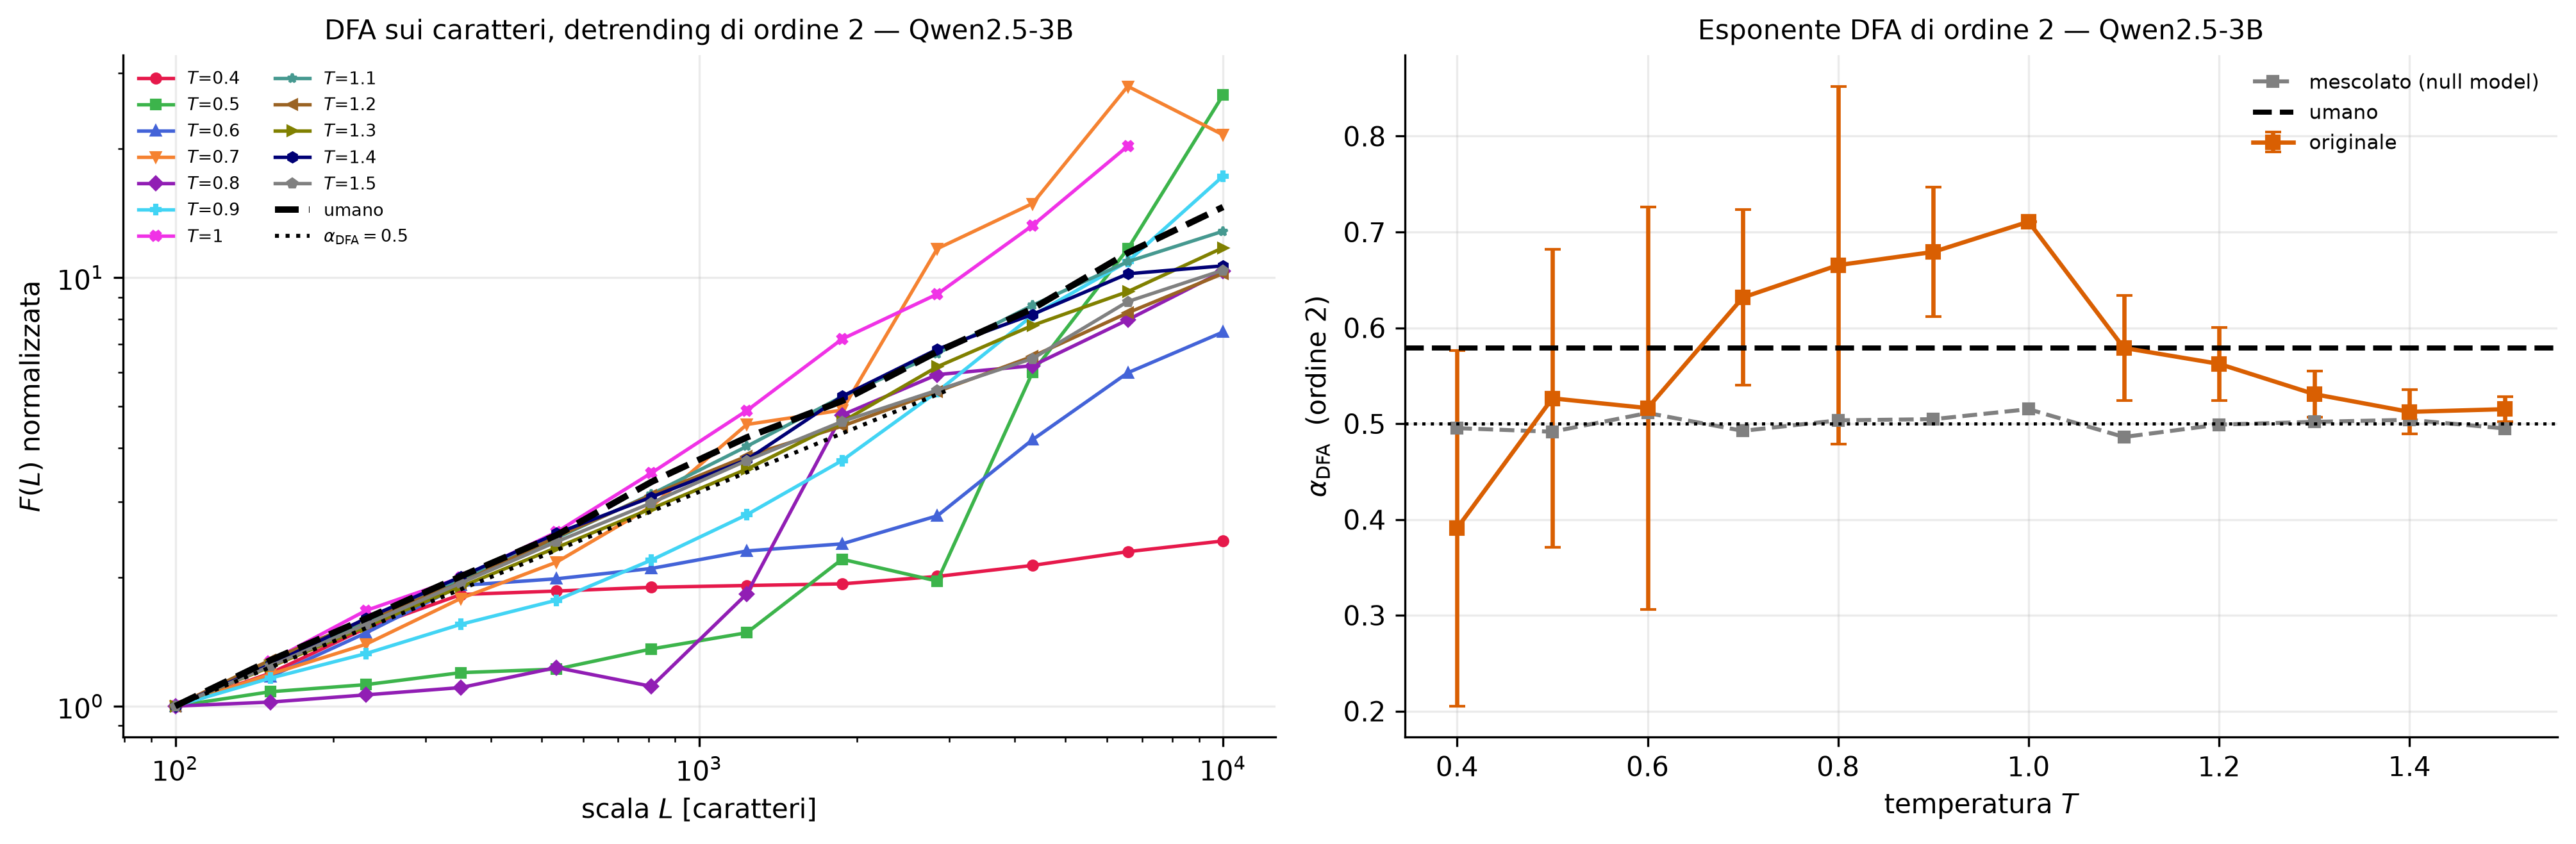
\includegraphics[width=\textwidth]{figure/cap4_dfa_Qwen25_3B_o2.png}
  \caption{Fluttuazione detrendizzata per il modello Qwen2.5-3B, con detrending
  quadratico. A sinistra $F(s)$ in funzione della scala, una curva per
  temperatura, con la pendenza di riferimento $\alpha_{\mathrm{DFA}} = 1/2$; a
  destra l'esponente in funzione della temperatura, con il null model
  rimescolato e la baseline umana.}
  \label{fig:dfa}
\end{figure}

\paragraph{La dispersione è il vero segnale.}
Il valore medio dell'esponente nasconde il fenomeno più informativo, ed è un
fenomeno già osservato: sulle reti LSTM~\cite{lippi2019} riporta che le stime
sui singoli campioni sono molto disperse attorno a $T = 0.5$ e strettamente
raccolte attorno alla media a $T = 1.0$. Gli stessi dati mostrano qui lo stesso
comportamento su architetture transformer. La deviazione standard fra documenti
passa da $0.219$ a $T = 0.4$ a $0.022$ a $T = 1.4$: alle basse temperature la
stima è dieci volte più dispersa. A $T = 0.4$ i cinque documenti del modello
esemplare danno esponenti compresi fra $0.16$ e $0.66$, cioè coprono
l'intervallo fra la saturazione e il valore umano; sull'insieme dei cinque
modelli l'escursione va da $0.07$ a $0.89$.

Questo comportamento è coerente con il caso limite discusso nel
§\ref{sec:ponte}. Quando il testo entra in un ciclo di ripetizione, il profilo
cumulato oscilla invece di allontanarsi dall'origine e la fluttuazione satura:
l'esponente crolla. Il crollo dipende però dalla lunghezza del ciclo rispetto
alle scale analizzate, che varia da documento a documento, e non tutti i testi
ripetitivi lo manifestano.

I dati permettono di precisare la relazione, che è a senso unico. Tutti e
diciannove i documenti con $\alpha_{\mathrm{DFA}} < 0.3$ si trovano a
$T \le 0.6$ e hanno una quota media di 8-grammi ripetuti pari a $0.984$: un
esponente collassato implica dunque ripetizione conclamata. Il viceversa non
vale: fra gli 82 documenti con quota di 8-grammi ripetuti superiore a $0.9$,
soltanto 33 hanno un esponente inferiore a $1/2$, e la correlazione di rango fra
le due quantità non è significativa
($\rho = +0.03$, $p = 0.61$). La ripetizione è quindi condizione necessaria ma
non sufficiente al collasso dell'esponente.

Ne segue una conseguenza metodologica. Alle basse temperature
$\alpha_{\mathrm{DFA}}$ non è un indicatore affidabile di correlazione a lungo
raggio, né lo è il suo valore medio; è la sua dispersione a segnalare il regime.
Il controllo sull'ordine del detrending riportato nel §\ref{sec:robustezza}
punta nella stessa direzione, poiché lo scarto fra i due ordini è massimo
proprio nell'intervallo $T \in [0.5, 0.8]$ e trascurabile altrove.

% ---------------------------------------------------------------------
\section{Entropia, divergenza dal testo umano e plagio}
\label{sec:entropia-risultati}

Le sezioni precedenti confrontano il testo generato con quello umano una misura
alla volta. La divergenza di Kullback--Leibler introdotta nel
§\ref{sec:crossparsing} permette invece un confronto diretto fra i due testi,
senza passare per un descrittore intermedio, ed è per questa ragione il criterio
più stringente del capitolo: non dipende da soglie teoriche né dalla scelta di
quale proprietà misurare.


La divergenza ha un minimo netto, che cade a $T = 0.9$ per quattro modelli su
cinque e a $T = 1.0$ per Qwen3.5-4B-Base. Nessuna delle \num{242} stime risulta
negativa, il che conferma sui dati reali la proprietà dello stimatore verificata
nel §\ref{sec:validazione}.

Il valore al minimo varia molto fra i modelli: $0.096$ bit per carattere per il
modello da 14 miliardi di parametri, $0.232$ e $0.245$ per i due Qwen3.5,
$0.321$ per il modello da 1.5 miliardi e $0.914$ per quello da 3 miliardi. La
posizione del minimo è dunque comune, la sua profondità no: fra il modello che
si avvicina di più al testo umano e quello che ci riesce meno corre quasi un
fattore dieci. La profondità non segue però la dimensione. La correlazione di
rango con il numero di parametri vale $\rho = -0.50$ con $p = 0.39$ su cinque
modelli, e il valore peggiore appartiene al modello da 3 miliardi anziché al più
piccolo: quanto un modello si avvicini al testo umano nel proprio punto migliore
è una proprietà del singolo modello, non della sua scala, almeno con la potenza
statistica qui disponibile. Vale inoltre la cautela imposta dal
§\ref{sec:robustezza}, poiché il modello da 14 miliardi dispone di un solo
campione per temperatura e il suo valore non è corredato da una stima della
dispersione.

L'entropia stimata per compressione mostra la transizione in modo ancora più
brusco. Per il modello esemplare la mediana vale $0.001$ bit per carattere
fino a $T = 0.8$, perché il testo ripetitivo è essenzialmente incomprimibile
oltre la prima occorrenza del ciclo e non trasporta informazione; sale poi a
$0.332$ in media a $T = 0.9$ e supera $4$ da $T = 1.0$ in poi, contro i $2.23$
del testo umano. Fra $T = 0.6$ e $T = 0.9$ la media si stacca dalla mediana
perché un documento per temperatura esce dal ciclo prima degli altri, e il
valore isolato di $5.77$ che il modello esemplare raggiunge a $T = 1.0$
proviene dall'unico documento sopravvissuto a quella temperatura: è la stessa
dispersione descritta nel §\ref{sec:dfa-risultati}, e conferma che nel regime
periodico il valore medio non descrive alcun documento. Il passaggio dal
regime a entropia trascurabile a quello a entropia superiore a quella umana si
consuma comunque entro due passi di temperatura.

% ---------------------------------------------------------------------
\section{Struttura misurata per compressione}
\label{sec:compressione-risultati}

Le misure basate su compressione del §\ref{sec:compressione} non richiedono di
scegliere un'unità di analisi né di stimare un esponente: operano direttamente
sui byte del testo. Costituiscono quindi un controllo indipendente da tutte le
scelte metodologiche discusse finora.

\begin{figure}[htbp]
  \centering
  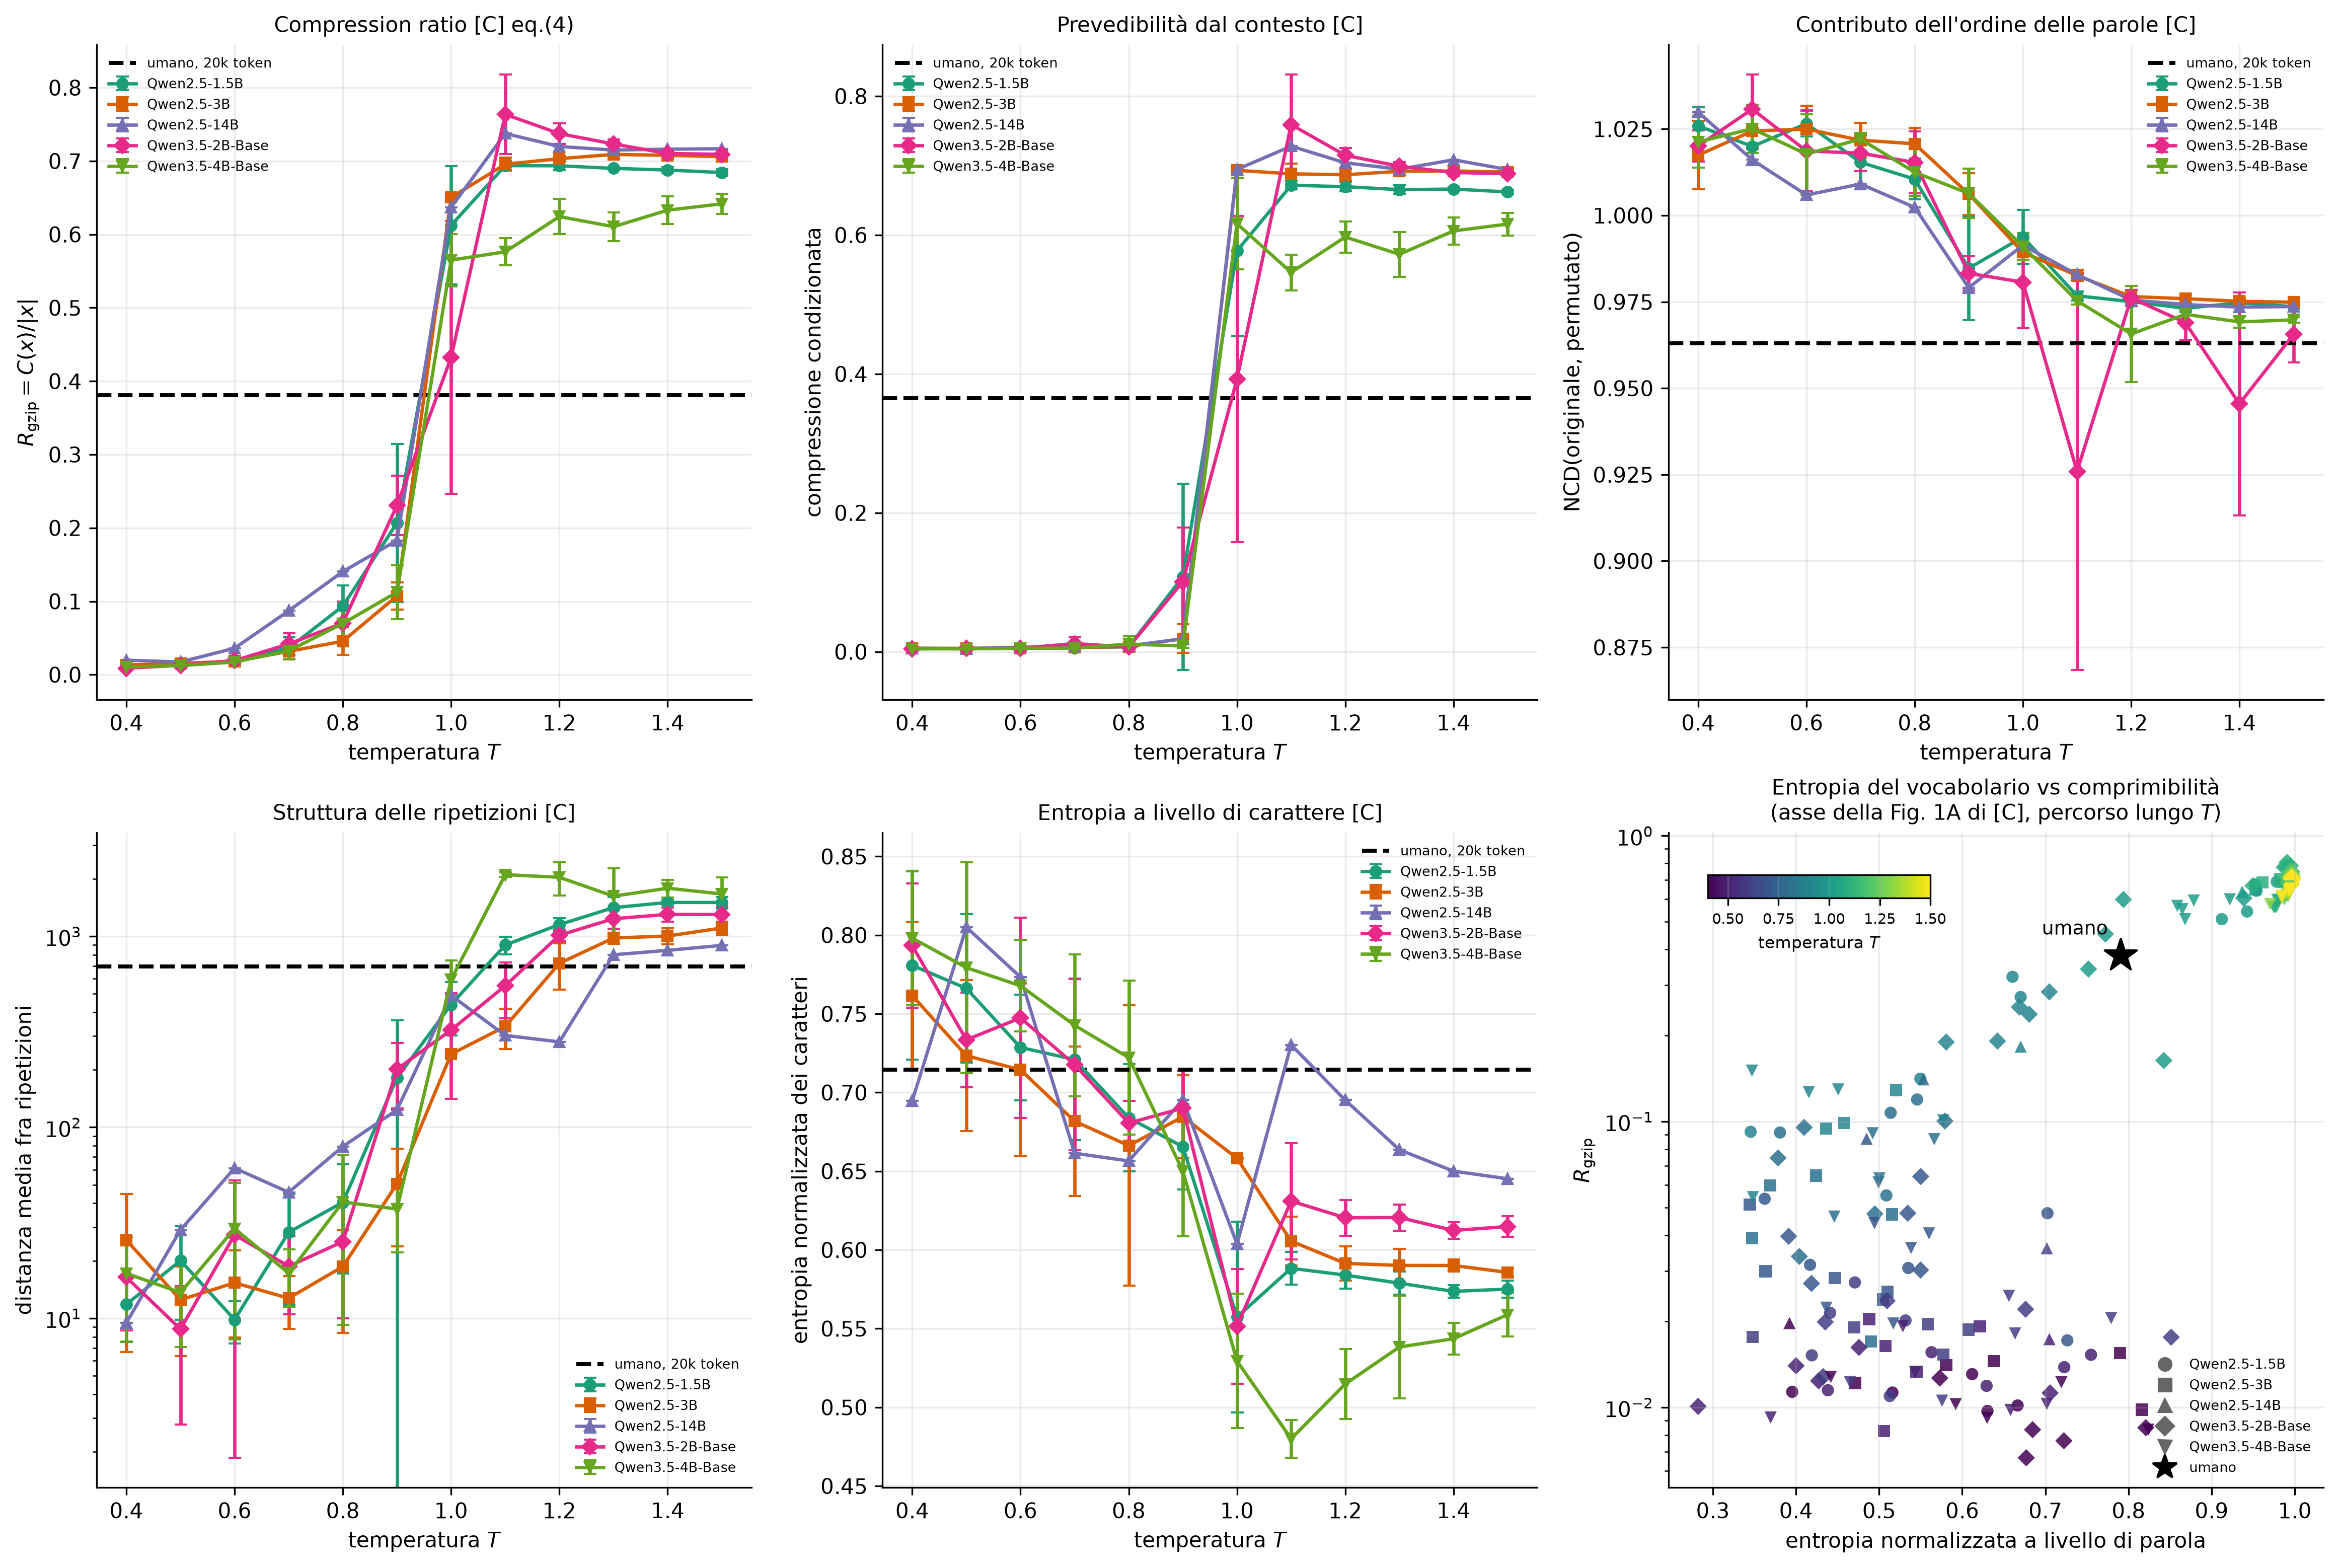
\includegraphics[width=\textwidth]{figure/cap4_compressione.png}
  \caption{Sei misure basate su compressione. Le prime cinque sono riportate in
  funzione della temperatura; l'ultima, in basso a destra, riporta il rapporto
  di compressione contro
  l'entropia normalizzata a livello di parola: è il piano della Figura~1A
  di~\cite{hadad2026}, percorso qui facendo variare la temperatura, con il testo
  umano segnato da una stella. In quel pannello il colore codifica la
  temperatura e la forma del marcatore il modello, e la scala verticale è
  logaritmica.}
  \label{fig:compressione}
\end{figure}

Il rapporto di compressione è la misura che separa i regimi in modo più netto di
tutte le altre. Per il modello esemplare passa da $0.013$ a $T = 0.4$ a $0.107$
a $T = 0.9$ e a $0.650$ a $T = 1.0$: un fattore cinquanta fra i due estremi, con
un salto di un fattore sei concentrato in un singolo passo di temperatura. Il
valore umano è $0.381$, e viene attraversato fra $T = 0.9$ e $T = 1.0$ come
tutte le altre misure del capitolo.

Il lavoro di~\cite{hadad2026} riporta che il testo generato è più regolare e
più comprimibile di quello umano, mentre qui il rapporto di compressione
supera il valore umano sopra $T = 1.0$. Le due osservazioni non sono in
contrasto, perché descrivono regioni diverse dello stesso asse: sotto la
transizione il testo generato è molto più comprimibile del testo umano,
$0.013$ contro $0.381$, ed è il regime in cui i modelli operano con le
impostazioni ordinarie; sopra la transizione la comprimibilità cade perché il
testo cessa di essere linguaggio, non perché acquisti struttura.

La compressione condizionata si comporta in modo analogo ma dice qualcosa di
diverso. Fino a $T = 0.9$ vale meno di $0.02$: la seconda metà del documento è
quasi interamente prevedibile dalla prima, come è ovvio in un testo che ripete
lo stesso ciclo. Da $T = 1.0$ sale a circa $0.69$, quasi il doppio del valore
umano $0.365$: la seconda metà è ora \emph{meno} prevedibile dalla prima di
quanto lo sia in un romanzo. Fra i due regimi non esiste una temperatura in cui
la predicibilità dal contesto assomigli a quella del testo umano.

Il salto oltre il valore umano non è una particolarità del modello esemplare. La
mediana su tutti e cinque i modelli passa da $0.015$ a $T = 0.9$ a $0.627$ a
$T = 1.0$, e il singolo modello che si avvicina di più al valore umano da sotto,
il Qwen3.5-2B-Base con $0.135$, lo scavalca comunque in un passo arrivando a
$0.430$. Nessuno dei cinque si ferma sul valore umano, ed è l'unica delle misure
di questo capitolo per cui ciò accade.

\paragraph{Il piano entropia--comprimibilità.}
Il pannello in basso a destra della Figura~\ref{fig:compressione} colloca i
documenti nel piano definito da~\cite{hadad2026}, percorso qui da un modello
reale al variare di un solo parametro anziché da distribuzioni artificiali, con
il testo umano in posizione intermedia. L'asse verticale è logaritmico perché il rapporto di compressione
non si annulla mai: il valore più basso osservato è $0.0067$. Su un asse
lineare esteso fino a $0.81$, però, i 57 documenti che stanno fra $0.007$ e
$0.020$, quasi un quarto del totale, si sovrappongono tutti sulla linea dello
zero, e la loro struttura interna scompare. In scala logaritmica si vede
invece che occupano un intervallo di entropia molto ampio, da $0.28$ a $0.85$,
e la ragione è che le due grandezze misurano cose diverse. Il rapporto di
compressione dipende dalla ripetizione della sequenza: un testo che ripete
sempre lo stesso ciclo si comprime a poco più dell'un per cento della sua
dimensione, qualunque sia il numero di parole che il ciclo contiene.
L'entropia normalizzata dipende invece dalla forma della distribuzione delle
frequenze su quel vocabolario ridotto, che conta fra 37 e 235 tipi distinti.
Un ciclo lungo e vario e un ciclo corto e povero sono ugualmente comprimibili
ma hanno entropie molto diverse: da qui la dispersione orizzontale della
nuvola a bassa comprimibilità.

\paragraph{La lunghezza del ciclo, misurata.}
L'argomento appena esposto invoca una grandezza che le misure di questo capitolo
non contengono, la lunghezza del ciclo ripetuto, ed è quindi il caso di
misurarla. Sulla successione di parole di ciascun documento si cerca il più
piccolo sfasamento $L_{\mathrm{ciclo}}$ per cui l'accordo fra la parola in
posizione $i$ e quella in posizione $i - L_{\mathrm{ciclo}}$, calcolato sugli
ultimi venti giri, supera il novanta per cento. La finestra di verifica è locale
e commisurata al periodo candidato: su tutto il testo la prosa che precede il
ciclo diluirebbe la media, mentre su un suffisso lungo un ciclo che cambia
lentamente variante scende sotto soglia al proprio periodo e la supera a un
multiplo, restituendo un alias. La soglia è fissata al novanta e non al cento
per cento per tollerare i cicli non esattamente verbatim; l'accordo atteso per
caso in prosa inglese è circa $0.05$, quindi non vi sono falsi positivi.

Il criterio individua \num{113} documenti su \num{242}, e sono tutti a
$T \le 0.9$: la totalità fino a $T = 0.7$, il $95\%$ a $T = 0.8$, il $56\%$ a
$T = 0.9$ e nessuno da
$T = 1.0$ in poi. Coincidono con la nuvola a bassa comprimibilità: tutti e
cinquantasette i documenti con $R_{\mathrm{gzip}} < 0.02$ sono fra questi. Il
ciclo va da una sola parola a \num{248}, in caratteri da $9$ a \num{1127}, con
mediana di $16$ parole.

La Figura~\ref{fig:ciclo} riporta la relazione con le due grandezze del piano.
Con l'entropia di parola la correlazione di rango vale $\rho = +0.65$, e non è
un effetto della temperatura: calcolata fra documenti generati alla stessa
temperatura sale a $+0.69$, ed è positiva in tutti e sei i gruppi. Con il
rapporto di compressione, invece, non c'è relazione: $\rho = -0.15$ con
$p = 0.12$, e a temperatura fissata il segno si inverte, $+0.16$ con
$p = 0.11$. A parità di lunghezza del ciclo il rapporto di compressione varia di
un fattore compreso fra quattordici e ventisette.

Il meccanismo è quello anticipato sopra, e la misura lo rende esplicito: la
lunghezza del ciclo coincide quasi con il numero di tipi distinti che esso
contiene, $\rho = +0.84$, cosicché un ciclo corto concentra tutta la massa di
probabilità su poche parole e uno lungo la distribuisce. Gli estremi lo
mostrano nel modo più diretto: il ciclo più corto osservato è una sola parola,
ripetuta, con entropia $0.35$; il più lungo conta \num{248} parole e undici
tipi distinti, \emph{You are a bad father. You are a bad lover of children.
You are not to blame} con variazioni, con entropia $0.47$ e $R_{\mathrm{gzip}}
= 0.019$, cioè testo ancora ultracomprimibile. La lunghezza del ciclo spiega
dunque l'ordinamento lungo l'asse orizzontale del piano, non tutta la sua
dispersione: la regressione su $\log L_{\mathrm{ciclo}}$ rende conto del
$42\%$ della varianza dell'entropia.

\begin{figure}[htbp]
  \centering
  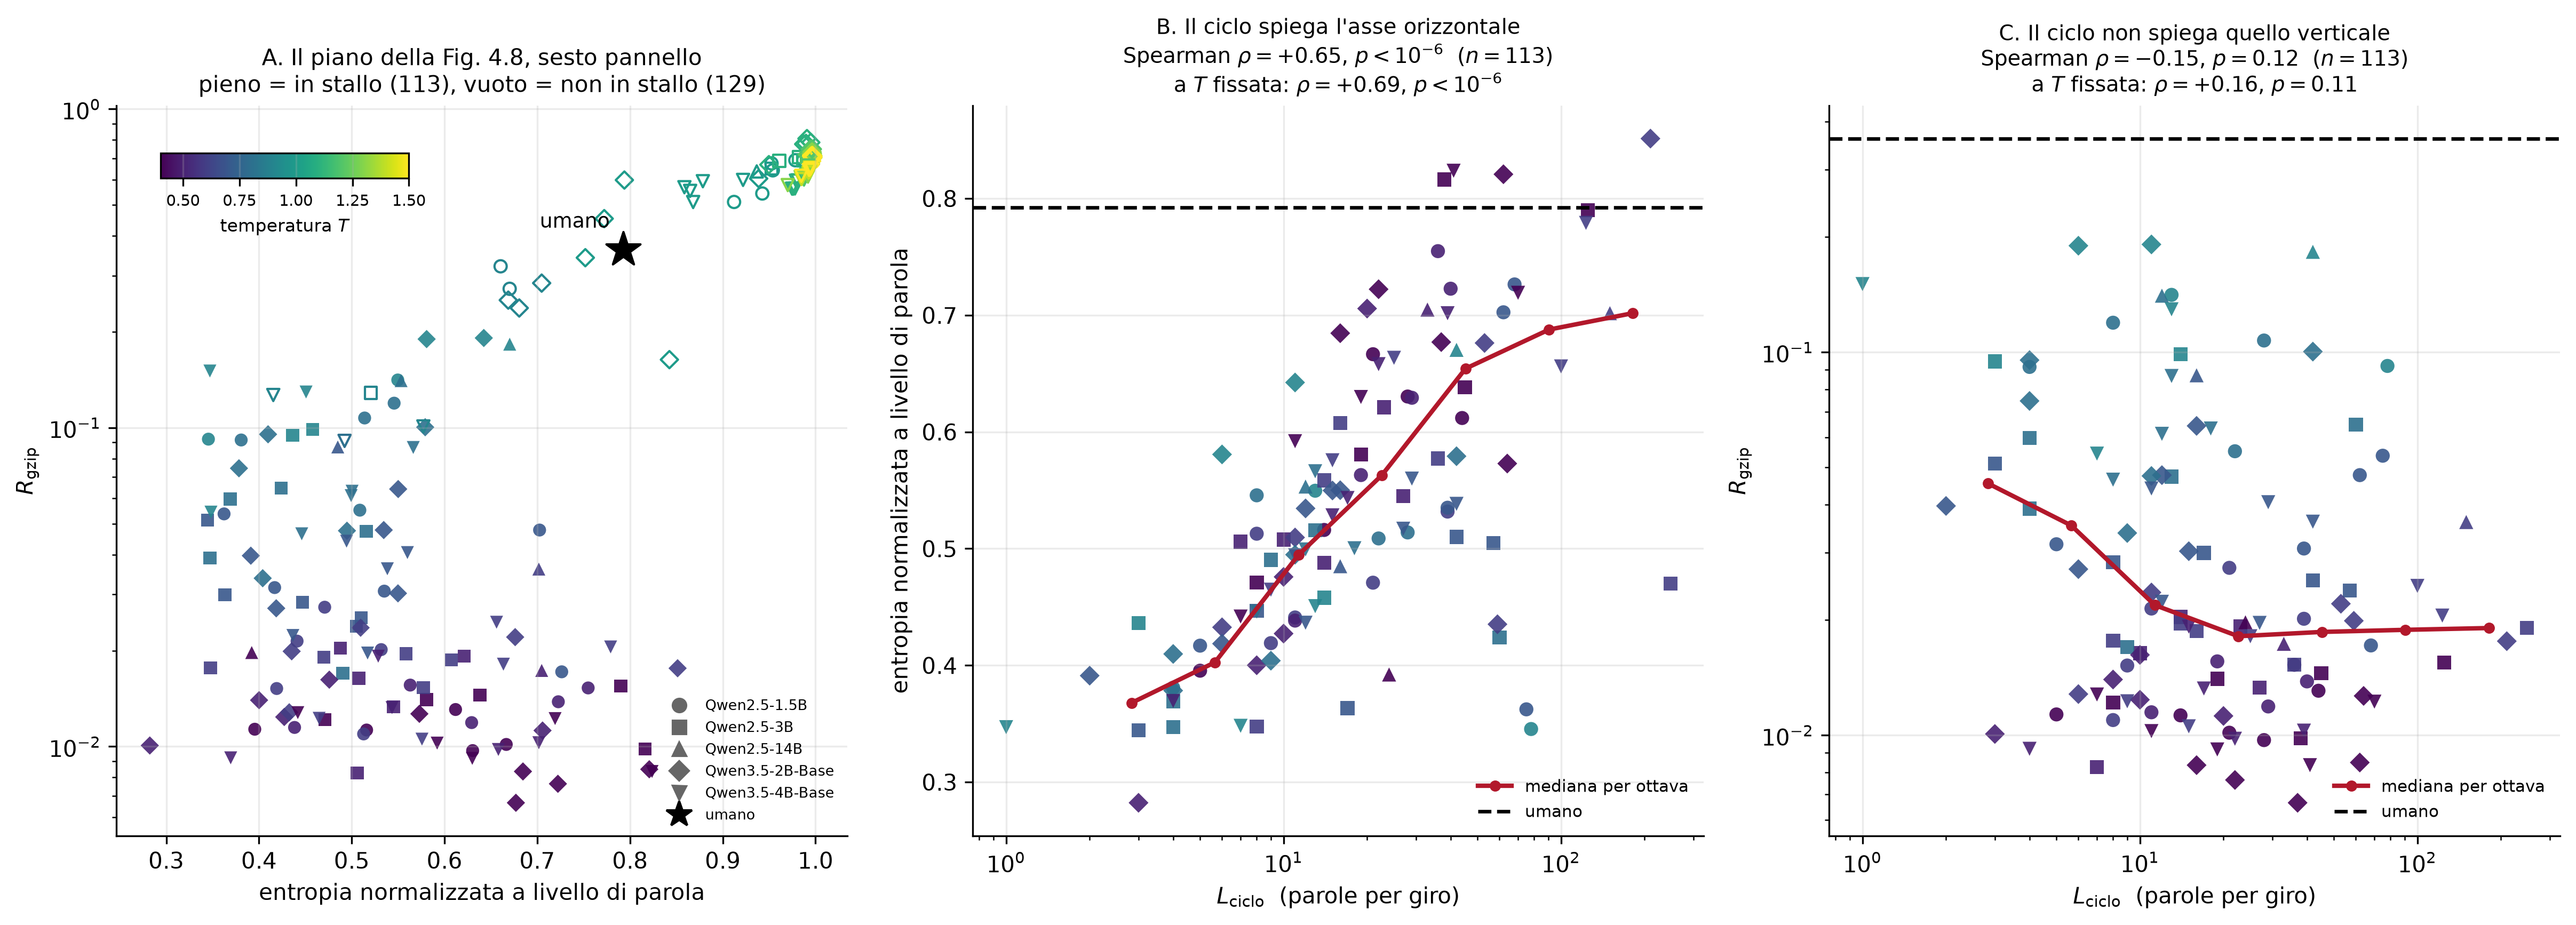
\includegraphics[width=\textwidth]{figure/cap4_ciclo_entropia.png}
  \caption{Lunghezza del ciclo ripetuto in fase di stallo. A: il piano
  entropia--comprimibilità della Figura~\ref{fig:compressione}, con i documenti
  in stallo a simbolo pieno e gli altri a simbolo vuoto; il colore codifica la
  temperatura e la forma il modello. B: entropia di parola contro lunghezza del
  ciclo, con la mediana per ottava. C: rapporto di compressione contro la stessa
  grandezza. La lunghezza del ciclo ordina l'asse orizzontale del piano e non
  quello verticale.}
  \label{fig:ciclo}
\end{figure}


% ---------------------------------------------------------------------
\section{Le tre fasi}
\label{sec:fasi-risultati}

Le misure precedenti descrivono il testo generato senza classificarlo. La regola
del §\ref{sec:tre-fasi} permette invece di assegnare ciascun documento a una
fase, e questa sezione ne riporta l'esito.

La traiettoria della~\eqref{eq:traiettoria} è costruita sui vettori GloVe a 100
dimensioni già impiegati nel §\ref{sec:token}, e l'autocorrelazione è calcolata
sui primi cento lag, misurati in parole. Il fit del GAPELMAPER usa invece un
intervallo più ampio, fino a 600 parole, perché distinguere una legge di potenza
da un esponenziale richiede più di una decade di distanze. Il livello di rumore
$\eta$ è stimato su una singola permutazione della traiettoria di ciascun
documento, con seme fissato.

Le due soglie della regola valgono $\kappa_{\min} = 0.50$ e $\Phi_{\min} = 3$.
La prima è deliberatamente permissiva: serve a escludere i documenti in cui meno
di metà delle parole ha un vettore, cioè quelli in cui la traiettoria è fatta per
lo più di zeri, e non a selezionare i documenti buoni. La seconda separa i due
gruppi in cui $\Phi$ effettivamente si distribuisce, e la sua posizione è poco
critica: come mostra la Figura~\ref{fig:transizioni}, fra la fase periodica e
quella successiva $\Phi$ cambia di due ordini di grandezza, cosicché qualunque
soglia compresa fra $1$ e $5$ produce la stessa classificazione. Il
§\ref{sec:tstar} riprende il punto trattando la fine della fase periodica come
uno degli otto criteri di temperatura critica.

La Figura~\ref{fig:acf} mostra come questa autocorrelazione cambia lungo lo
sweep. Fino a $T = 0.9$ la curva oscilla con periodo definito e ampiezza
prossima all'unità: il testo ripete un ciclo di parole, e a distanza pari a un
multiplo del ciclo ogni vettore ritrova sé stesso. Il periodo si accorcia al
crescere della temperatura, da dieci parole a $T = 0.5$ a circa tre a $T =
0.8$, mentre l'ampiezza scende da $0.98$ a $0.72$. Fra $T = 0.9$ e $T = 1.0$
la struttura periodica scompare del tutto: l'ampiezza cade a $0.036$ e la
curva diventa un decadimento monotono, senza più oscillazione. A $T = 1.3$
l'intera curva è contenuta nella banda di rumore stimata mescolando le parole
del documento, cioè non è distinguibile dal caso.

Il confronto con il testo umano chiarisce quanto entrambi i regimi siano
lontani dal linguaggio naturale. L'autocorrelazione del romanzo non è
periodica, con $\max\lvert\mathrm{FFT}\rvert$ pari a $1.16$, ben sotto la
soglia $3$, ma è nettamente sopra il livello di rumore su tutti i cento lag
esaminati, e il suo spettro decade in modo regolare invece di essere piatto.
Nessuna delle temperature campionate riproduce questa combinazione: sotto la
transizione la correlazione è troppo forte e periodica, sopra è assente.

\begin{figure}[htbp]
  \centering
  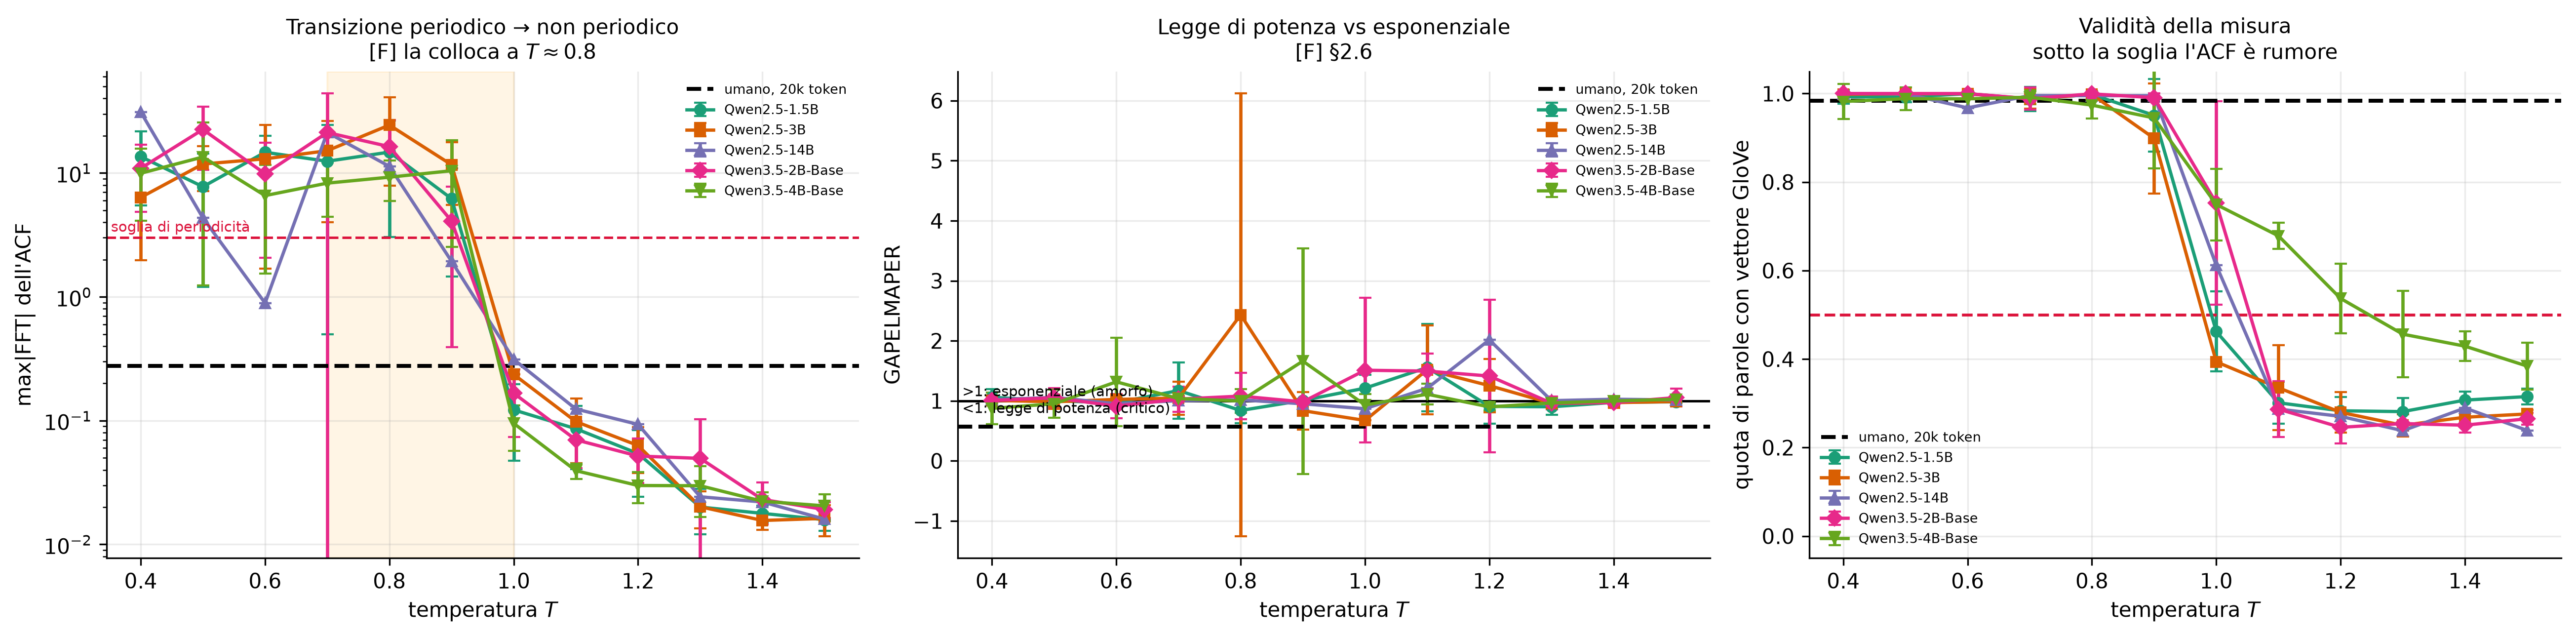
\includegraphics[width=\textwidth]{figure/cap4_transizioni_fase.png}
  \caption{Parametro di periodicità, GAPELMAPER e copertura degli embedding in
  funzione della temperatura. Il primo pannello è in scala logaritmica. Il terzo
  riporta la quota di parole dotate di un vettore, che è la condizione di
  validità delle altre due misure.}
  \label{fig:transizioni}
\end{figure}

\begin{figure}[htbp]
  \centering
  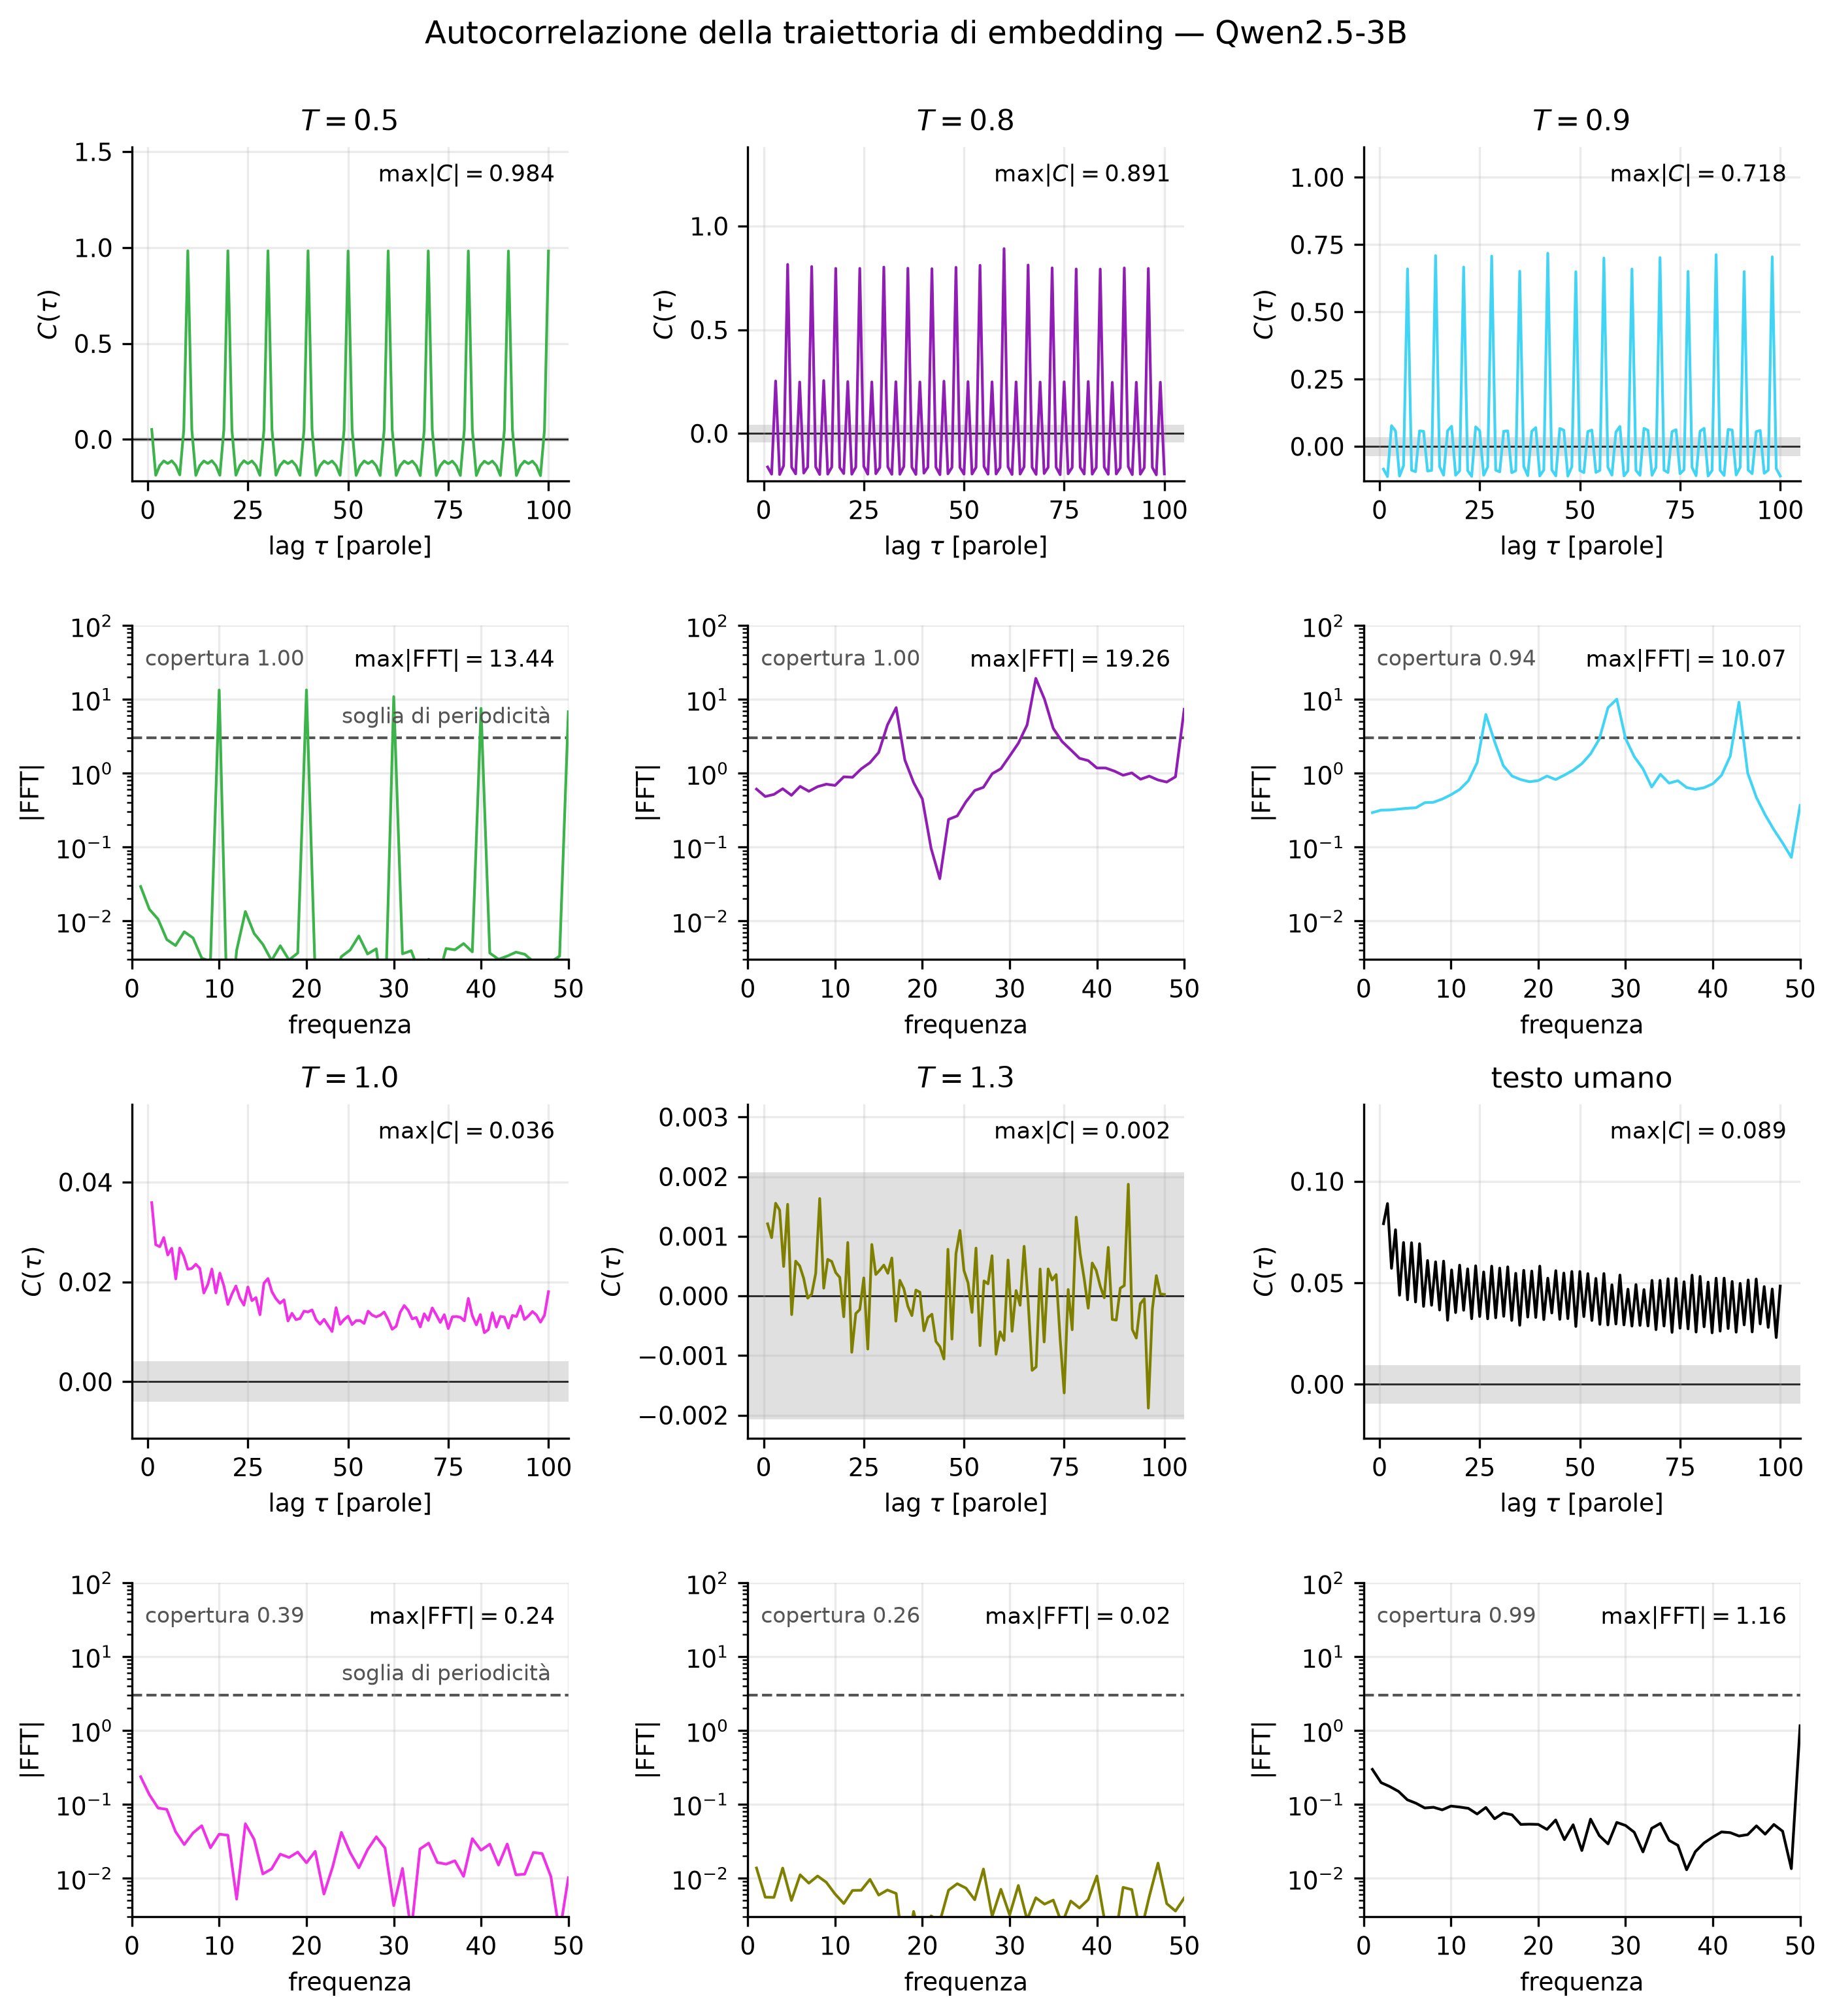
\includegraphics[width=\textwidth]{figure/cap4_acf_Qwen25_3B.png}
  \caption{Autocorrelazione della traiettoria di embedding per il modello
  Qwen2.5-3B a cinque temperature e sul testo umano di riferimento. In ciascuna
  coppia di riquadri il primo riporta $C(\tau)$ per lag da 1 a 100 parole e il
  secondo il modulo della sua trasformata di Fourier. La banda grigia è il
  livello di rumore, stimato ricalcolando $C(\tau)$ dopo aver permutato a caso
  le parole dello stesso documento; la linea tratteggiata è la soglia
  $\max\lvert\mathrm{FFT}\rvert = 3$ che separa la fase periodica. Per ogni
  temperatura è mostrato il campione di periodicità mediana, non il più marcato.
  La scala verticale di $C(\tau)$ è propria di ciascun riquadro, perché
  l'ampiezza varia di oltre due ordini di grandezza fra le temperature basse e
  quelle alte; il valore di picco è riportato dentro il riquadro. La scala dello
  spettro è invece logaritmica e comune, così i sei casi si confrontano
  direttamente.}
  \label{fig:acf}
\end{figure}

Il parametro d'ordine della prima transizione è il massimo modulo della
trasformata oltre il primo coefficiente, e il suo crollo è il risultato più
netto dell'intero capitolo. La media su tutti i modelli vale $16.0$ a
$T = 0.8$, scende a $7.5$ a $T = 0.9$ e precipita a $0.145$ a $T = 1.0$: un
fattore cinquanta in un solo passo di temperatura, e cento rispetto al massimo
di $T = 0.8$. Prosegue poi fino a $0.018$ a
$T = 1.5$, complessivamente tre ordini di grandezza sotto il massimo. Le cinque
curve dei diversi modelli si sovrappongono quasi esattamente, come mostra la
Figura~\ref{fig:transizioni}.

Anche questa soglia va confrontata con la fonte.
In~\cite{mikhaylovskiy2025states} la transizione dalla fase periodica è
collocata attorno a $t = 0.8$, con il testo dichiarato già non periodico a
$t = 1$, mentre qui la periodicità sopravvive fino a $T = 0.9$ e scompare a
$T = 1.0$. Lo spostamento verso l'alto è coerente con l'effetto del prompt
descritto nel §\ref{sec:protocollo}, che ritarda la comparsa delle proprietà
del regime disordinato.

\paragraph{Il secondo criterio non discrimina.} La distinzione fra stato
critico e fase amorfa dovrebbe essere operata dal GAPELMAPER, ma sui dati di
questo lavoro tale criterio non funziona. Il suo valore medio è $1.101$ con
deviazione standard $0.677$, e la quota di documenti con valore inferiore a 1,
cioè classificati come critici, è $0.51$: una moneta. Le barre d'errore nel
pannello centrale della Figura~\ref{fig:transizioni} sono di ampiezza
confrontabile con l'intero intervallo di variazione.

La difficoltà non è propria di questi dati. Lo stesso
\cite{mikhaylovskiy2025states} riporta che sui testi Qwen il GAPELMAPER è
raramente inferiore a 1, e che a diverse temperature del suo sweep non è
calcolabile affatto perché l'autocorrelazione assume valori negativi. Il
criterio, insomma, discrimina male anche nel lavoro che lo introduce.

Il motivo emerge dal terzo pannello. La copertura degli embedding resta sopra il
$95\%$ fino a $T = 0.9$, ma crolla a $0.64$ a $T = 1.0$ e a circa $0.31$ oltre
$T = 1.2$: nel regime in cui il GAPELMAPER dovrebbe distinguere le ultime due
fasi, l'autocorrelazione è calcolata su una minoranza delle parole e non
contiene più segnale. Per questa ragione i documenti che non superano la soglia
di copertura sono marcati come non valutabili anziché classificati, come
anticipato nel §\ref{sec:tre-fasi}. Senza tale precauzione il criterio avrebbe
assegnato una fase a documenti in cui non c'è nulla da misurare.

\paragraph{Il diagramma di fase.}
La Figura~\ref{fig:diagramma} riporta la composizione delle fasi per modello e
temperatura. Il quadro è coerente su tutti e cinque: fase periodica fino a
$T = 0.9$, dove la classificazione è ancora periodica per 13 documenti su 18;
scomparsa completa della periodicità a $T = 1.0$; documenti prevalentemente non
valutabili da $T = 1.1$ in poi, e completamente tali a $T \ge 1.4$.

\begin{figure}[htbp]
  \centering
  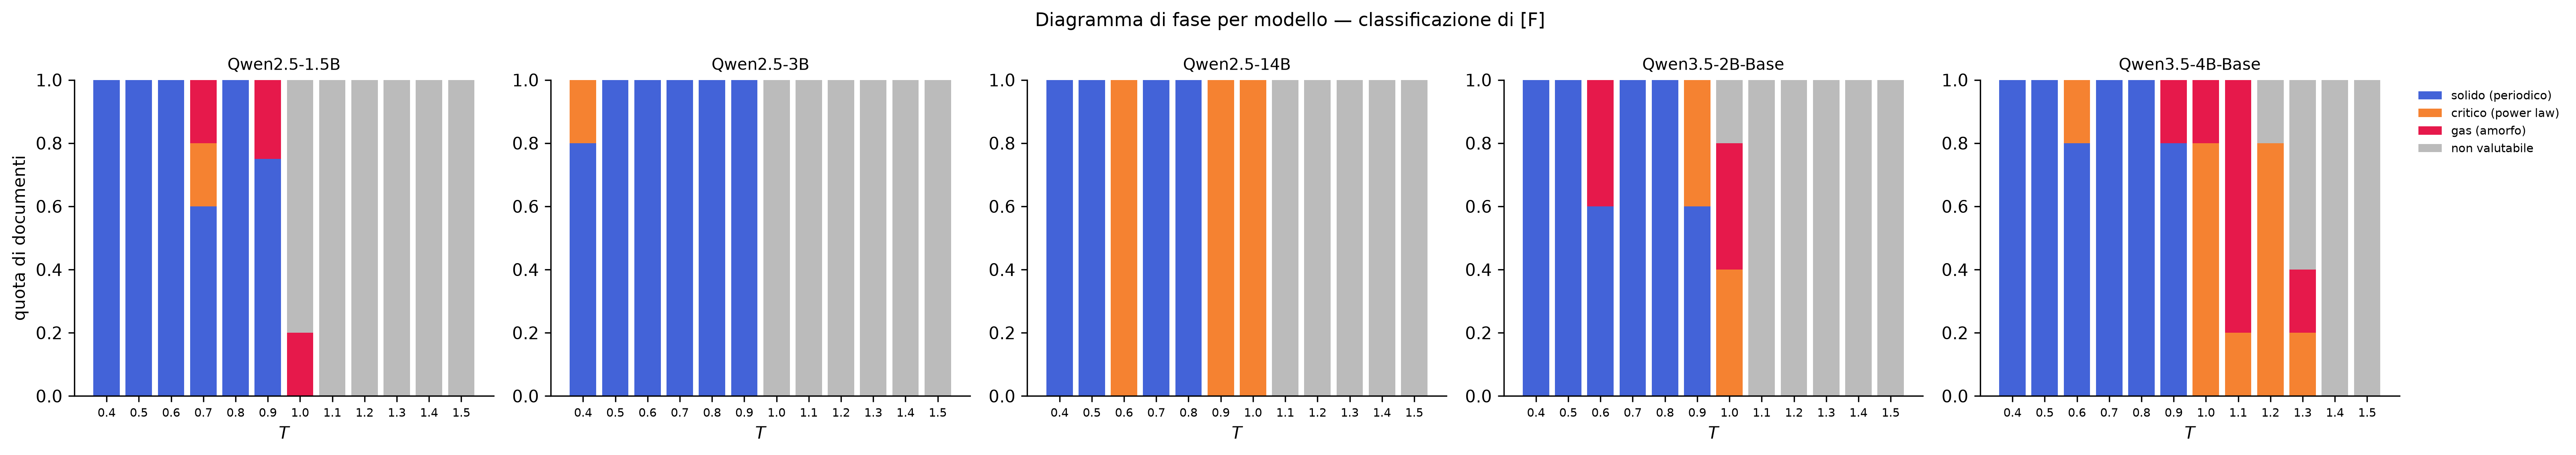
\includegraphics[width=\textwidth]{figure/cap4_diagramma_fase.png}
  \caption{Composizione delle fasi per modello e temperatura. La categoria «non
  valutabile» raccoglie i documenti che non superano la soglia di copertura
  degli embedding.}
  \label{fig:diagramma}
\end{figure}

Le tre modalità di fallimento del §\ref{sec:fallimenti} trovano qui la loro
interpretazione. La degenerazione per ripetizione è la fase periodica; la
degenerazione dell'alfabeto e del lessico corrisponde alla regione in cui la
misura non è più applicabile, che è a sua volta il segnale della fase amorfa. Il
testo non degenerato esiste solo nella striscia sottile fra le due, ed è la
stessa striscia in cui tutte le misure delle sezioni precedenti si avvicinano ai
valori umani.

% ---------------------------------------------------------------------
\section{Convergenza della temperatura critica}
\label{sec:tstar}

Le sezioni precedenti individuano ciascuna una temperatura privilegiata. Poiché
i criteri provengono da lavori indipendenti e misurano proprietà diverse del
testo, il loro accordo o disaccordo è esso stesso un risultato.

La Tabella~\ref{tab:tstar} riporta la temperatura selezionata da ciascun
criterio per ciascun modello. Due criteri sono intrinseci, nel senso che
individuano un estremo della curva senza far riferimento al testo umano: il
minimo del MAPE e la fine della fase periodica. Gli altri sei selezionano la
temperatura alla quale la misura si avvicina di più alla baseline umana.

\begin{table}[htbp]
\centering
\small
\begin{tabular}{@{}lccccc@{}}
\toprule
Criterio & 1.5B & 3B & 14B & 3.5-2B & 3.5-4B \\
\midrule
MAPE minimo                                  & 0.9 & 0.9 & 0.7 & 0.9 & 0.9 \\
$D_s$ minima dal testo umano                 & 0.9 & 0.9 & 0.9 & 0.9 & 1.0 \\
Fine della fase periodica                    & 1.0 & 1.0 & 0.6 & 1.0 & 1.0 \\
$R_{\mathrm{gzip}}$ più vicino all'umano     & 0.9 & 1.0 & 0.9 & 1.0 & 1.0 \\
$\alpha$ più vicino all'umano                & 1.0 & 1.5 & 1.3 & 1.0 & 1.0 \\
$R$ più vicino all'umano                     & 1.0 & 1.1 & 1.1 & 1.1 & 1.0 \\
$\gamma_H$ più vicino all'umano              & 1.1 & 1.0 & 1.3 & 1.1 & 1.3 \\
$\alpha_{\mathrm{DFA}}$ più vicino all'umano & 1.2 & 1.1 & 1.1 & 1.1 & 1.1 \\
\midrule
\textbf{mediana}                             & \textbf{1.0} & \textbf{1.0} &
\textbf{1.0} & \textbf{1.0} & \textbf{1.0} \\
\bottomrule
\end{tabular}
\caption{Temperatura selezionata da ciascun criterio, per ciascun modello. La
mediana vale $1.0$ per tutti e cinque i modelli, benché i singoli criteri
spazino da $0.6$ a $1.5$.}
\label{tab:tstar}
\end{table}

Il risultato principale del capitolo è la riga in fondo alla tabella. Otto
criteri tratti da quattro lavori indipendenti, costruiti per scopi diversi e mai
progettati per concordare, danno una mediana identica per tutti e cinque i
modelli. La convergenza non era scontata: i criteri misurano la distribuzione
delle frequenze, la crescita del vocabolario, le correlazioni a lungo raggio, la
comprimibilità e la periodicità dell'autocorrelazione, cioè proprietà che nulla
obbliga a coincidere.

\begin{figure}[htbp]
  \centering
  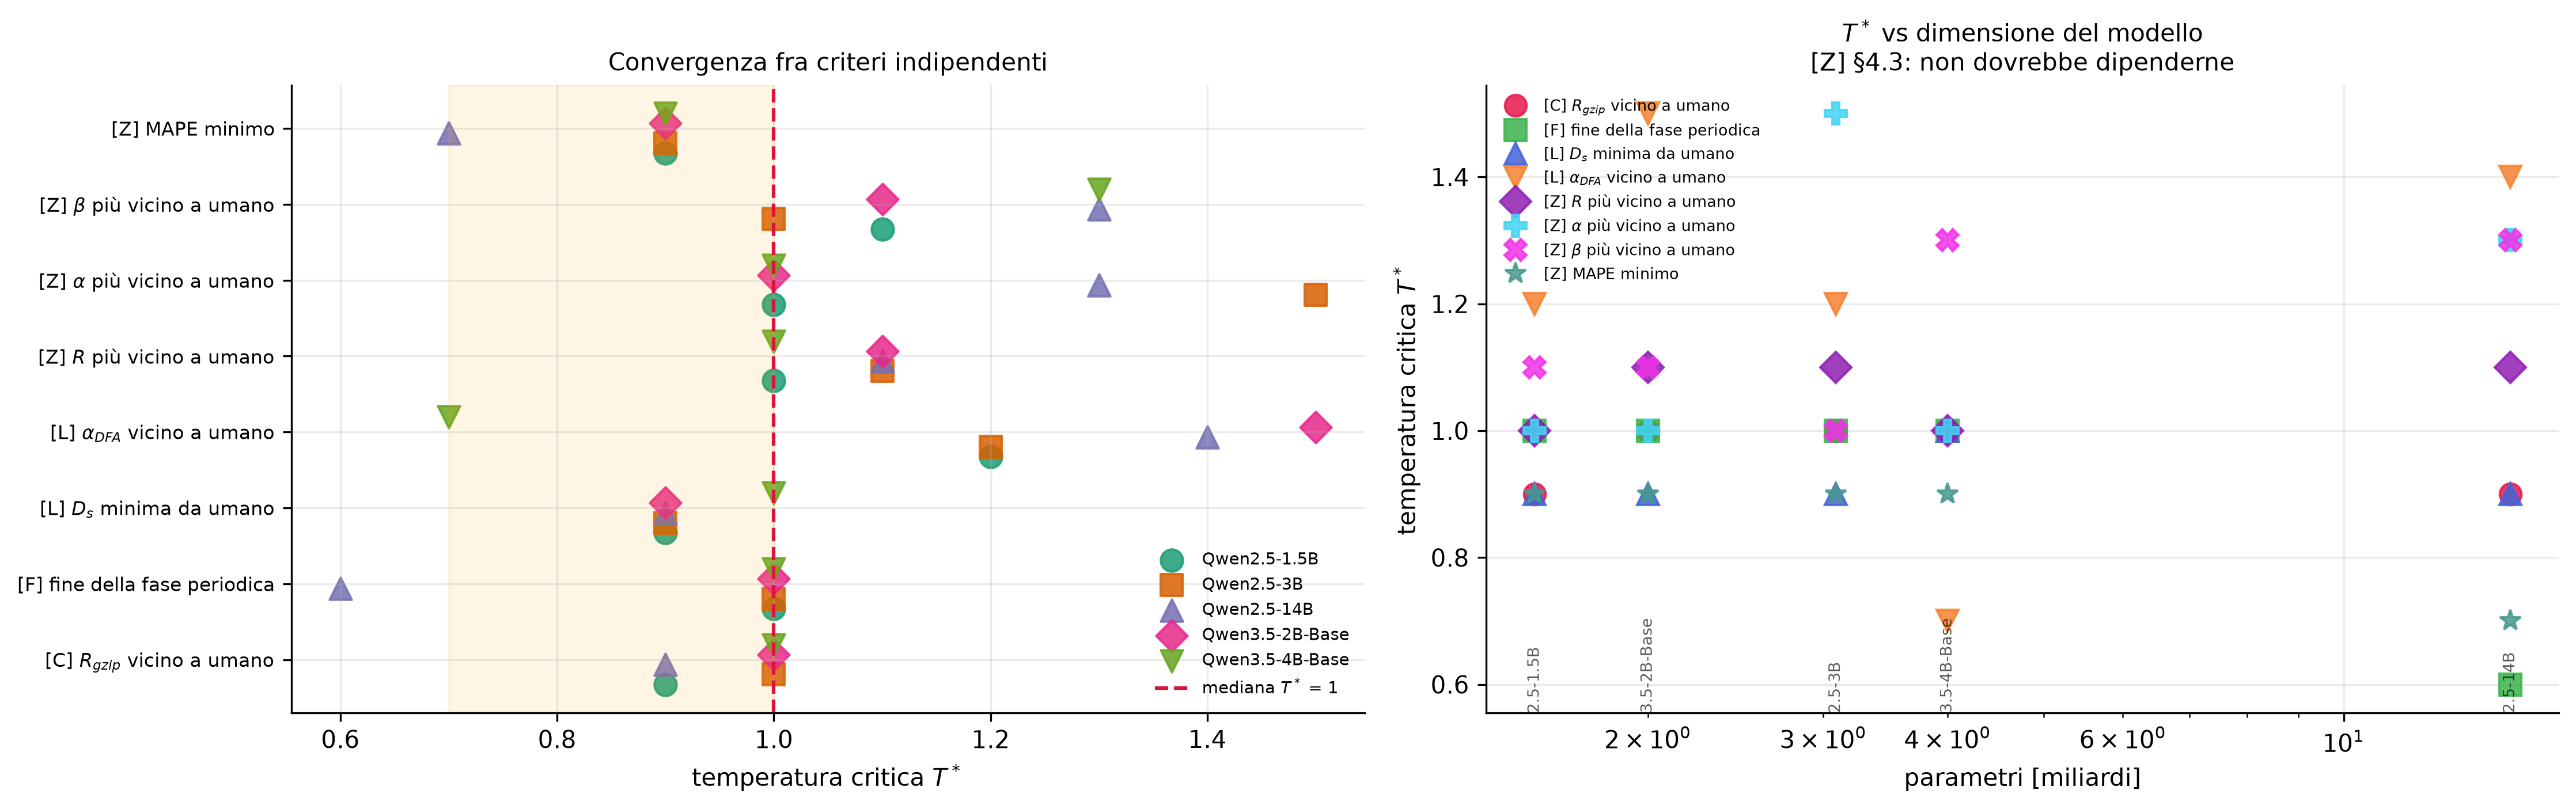
\includegraphics[width=\textwidth]{figure/cap4_temperatura_critica.png}
  \caption{A sinistra, la temperatura selezionata da ciascun criterio; la linea
  tratteggiata è la mediana complessiva e la banda la regione fra $0.7$ e $1.0$.
  A destra, la stessa quantità in funzione del numero di parametri del modello.}
  \label{fig:tstar}
\end{figure}

\paragraph{Dipendenza dalla dimensione del modello.}
La Figura~\ref{fig:tstar} riporta a destra la temperatura critica in funzione
del numero di parametri. La correlazione di rango è $\rho = -0.01$ con
$p = 0.93$ su quaranta osservazioni: nessuna dipendenza rilevabile. Il dato è
coerente con quanto riportato in~\cite{mikhaylovskiy2025zipf}, dove la posizione
dell'ottimo risulta indipendente dalla dimensione per tutte le famiglie
esaminate.

Un'assenza di correlazione misurata su cinque modelli appartenenti a due
famiglie non dimostra l'indipendenza: dimostra che, entro l'intervallo di
dimensioni esplorato e con la potenza statistica disponibile, non emerge
alcuna dipendenza. È coerenza con la letteratura, non conferma indipendente.

\paragraph{Una discordanza fra criteri.}
Due criteri si collocano sistematicamente fuori dal gruppo, e la loro distanza
dagli altri è essa stessa un risultato: mediarli insieme al resto la
cancellerebbe.

Il minimo del MAPE cade a $0.9$, mentre la fine della fase periodica cade a
$1.0$: alla temperatura in cui la distribuzione delle frequenze è più vicina a
una legge di potenza, l'autocorrelazione è ancora periodica per la maggioranza
dei documenti. Le due misure non si contraddicono, perché guardano oggetti
diversi, la statistica dei conteggi l'una e la struttura sequenziale l'altra,
e la loro distanza quantifica il fatto che le due proprietà non compaiono
simultaneamente. Il testo acquista una distribuzione di frequenze verosimile
prima di perdere la ripetizione.

Il criterio basato su $\alpha_{\mathrm{DFA}}$ merita una nota, perché il suo
esito dipende dall'ordine del detrending. Con il grado 1 seleziona temperature
fra $0.7$ e $1.5$, il più disperso dei nove; con il grado 2, che è quello
adottato qui per la ragione data nel §\ref{sec:robustezza}, si allinea agli
altri e sceglie $1.1$ per quattro modelli su cinque. La mediana per modello vale
$1.0$ in entrambi i casi. Resta valida l'avvertenza del
§\ref{sec:dfa-risultati}: alle basse temperature quell'esponente è instabile
fra documenti, e viene riportato per completezza anziché usato come criterio a
sé stante.

Una divergenza analoga fra criteri è documentata
in~\cite{mikhaylovskiy2025zipf} per i modelli Llama di grandi dimensioni, dove
le leggi di Zipf e di Heaps individuano temperature critiche sensibilmente
diverse. Il fenomeno non sembra dunque un artefatto di questo lavoro.

% ---------------------------------------------------------------------
\section{Che cosa lo sweep ha stabilito}
\label{sec:sintesi-cap4}

Tre risultati emergono dalle sezioni precedenti, di natura diversa fra loro.

Il primo è l'esistenza di una temperatura privilegiata, e la sua posizione. Otto
criteri costruiti per scopi diversi e tratti da quattro lavori indipendenti
danno una mediana identica, $T = 1.0$, per tutti e cinque i modelli, senza
dipendenza rilevabile dalla dimensione. Il secondo è che l'ottimo è stretto: la
transizione si consuma quasi interamente fra $T = 0.9$ e $T = 1.0$, dove il
parametro di periodicità cade di un fattore cinquanta, l'entropia passa da
$0.332$ a $5.77$ bit per carattere e il rapporto di compressione da $0.107$ a
$0.650$. Uno sweep a passo $0.1$ è appena sufficiente a risolvere quella
finestra.

Il terzo è l'esito negativo su cui poggia il capitolo successivo. L'esistenza
dell'ottimo è un fatto generale, ma la sua \emph{qualità} non lo è: due modelli
su cinque portano il MAPE al livello del testo umano e gli altri no. La
compressione condizionata non raggiunge il valore umano a nessuna temperatura,
ma per una ragione che non riguarda la struttura semantica: sotto la transizione
il testo ripete un ciclo e la seconda metà è prevedibile per costruzione, sopra
non è più linguaggio e non è prevedibile da nulla. Soprattutto, i documenti che
superano tutte e tre le soglie di non
degenerazione sono due su \num{242}. Il corpus generato lungo lo sweep non
sostiene quindi un'analisi semantica, ed è la ragione per cui il
Capitolo~\ref{cap:risultati2} cambia dominio anziché proseguire su questo.

Il capitolo non stabilisce però tutto. La convergenza dei criteri dice dove il
testo generato somiglia di più a quello umano secondo misure che ignorano il
significato; non dice se in quel punto il testo sia organizzato attorno a un
contenuto. È la domanda posta nel §\ref{sec:intro-domanda}, e richiede gli
strumenti del §\ref{sec:burst}.
%  Figure del corpo: modello Qwen2.5-3B. Quelle degli altri quattro
%  modelli stanno nel repository indicato in Appendice A.
% =====================================================================

\chapter{Il testo generato lungo lo sweep di temperatura}
\label{cap:risultati1}

Questo capitolo applica ai \num{242} documenti generati le misure introdotte nel
Capitolo~\ref{cap:teoria}, facendo variare la sola temperatura di campionamento.
Ogni misura viene confrontata con la baseline umana della
Tabella~\ref{tab:baseline}, calcolata con le stesse procedure e alla stessa
lunghezza.

Le figure del corpo del capitolo mostrano il modello Qwen2.5-3B, scelto come
esemplare perché dispone di cinque campioni per quasi tutte le temperature e
presenta le curve meno rumorose; le corrispondenti figure per gli altri quattro
modelli sono depositate nel repository indicato
nell'Appendice~\ref{app:codice}. Le curve aggregate
riportano invece tutti e cinque i modelli.

Il risultato principale non è nessuna delle singole misure, ma il fatto che
convergano: criteri tratti da quattro lavori indipendenti, costruiti per scopi
diversi, individuano la stessa regione di temperature. Il §\ref{sec:tstar} lo
documenta.

% ---------------------------------------------------------------------
\section{Le tre modalità di fallimento}
\label{sec:fallimenti}

La prima e la terza riga della Tabella~\ref{tab:tre-regimi} sono entrambe
prodotte dai modelli qui analizzati, a due temperature diverse, e mostrano i
due modi in cui la generazione si allontana dal linguaggio: la ripetizione letterale a bassa
temperatura, l'incoerenza semantica ad alta temperatura. Salendo ancora si
incontra un terzo regime, in cui l'alfabeto stesso si disgrega e il testo diventa
un miscuglio di sistemi di scrittura diversi.

Le tre modalità possono essere separate quantitativamente. Un documento viene
classificato come degenerato per \emph{ripetizione} se la quota di 8-grammi
ripetuti supera $0.10$, contro il valore $0.000$ misurato sul testo umano; come
degenerato nell'\emph{alfabeto} se la quota di caratteri non ASCII supera
$0.05$, più del triplo del valore umano $0.014$; come degenerato nel
\emph{lessico} se meno del $70\%$ delle sue parole possiede un vettore nello
spazio di embedding, contro il $98\%$ del testo umano. Le tre condizioni non si
escludono a vicenda, e un documento può soddisfarne più di una.

La Tabella~\ref{tab:fallimenti} riporta i conteggi.

\begin{table}[htbp]
\centering
\small
\begin{tabular}{@{}l>{\raggedright\arraybackslash}p{5.4cm}rr@{}}
\toprule
Modalità & Criterio & Documenti & Quota \\
\midrule
Ripetizione & 8-grammi ripetuti $> 0.10$      & 122 & 50\,\% \\
Alfabeto    & caratteri non ASCII $> 0.05$    & 125 & 52\,\% \\
Lessico     & copertura degli embedding $< 0.70$ & 112 & 46\,\% \\
\midrule
Nessuna     & prosa inglese non degenerata    &   2 &  1\,\% \\
\bottomrule
\end{tabular}
\caption{Modalità di degenerazione dei \num{242} documenti generati. Le
categorie non sono disgiunte. La classificazione dipende dalle soglie scelte,
ma non nella sostanza: facendole variare entro intervalli ragionevoli il numero
di documenti non degenerati resta compreso fra 2 e 7, cioè fra l'uno e il tre
per cento del totale.}
\label{tab:fallimenti}
\end{table}

Il dato va letto con attenzione, perché è il presupposto dell'intera seconda
parte sperimentale. Non significa che i modelli siano incapaci di produrre
linguaggio, ma che la finestra di temperature in cui lo producono è
sufficientemente stretta da non essere coperta da uno sweep a passo $0.1$: i
soli due documenti non degenerati compaiono a $T = 1.0$, e già a $T = 0.9$ e
$T = 1.1$ tutti i campioni ricadono in almeno una delle tre categorie. Il
Capitolo~\ref{cap:risultati2} muove da questa constatazione.


% ---------------------------------------------------------------------
\section{Legge di Zipf}
\label{sec:zipf-risultati}

La Figura~\ref{fig:zipf-cum} riporta gli istogrammi cumulativi delle frequenze,
una curva per temperatura, con la curva umana per confronto.

\begin{figure}[htbp]
  \centering
  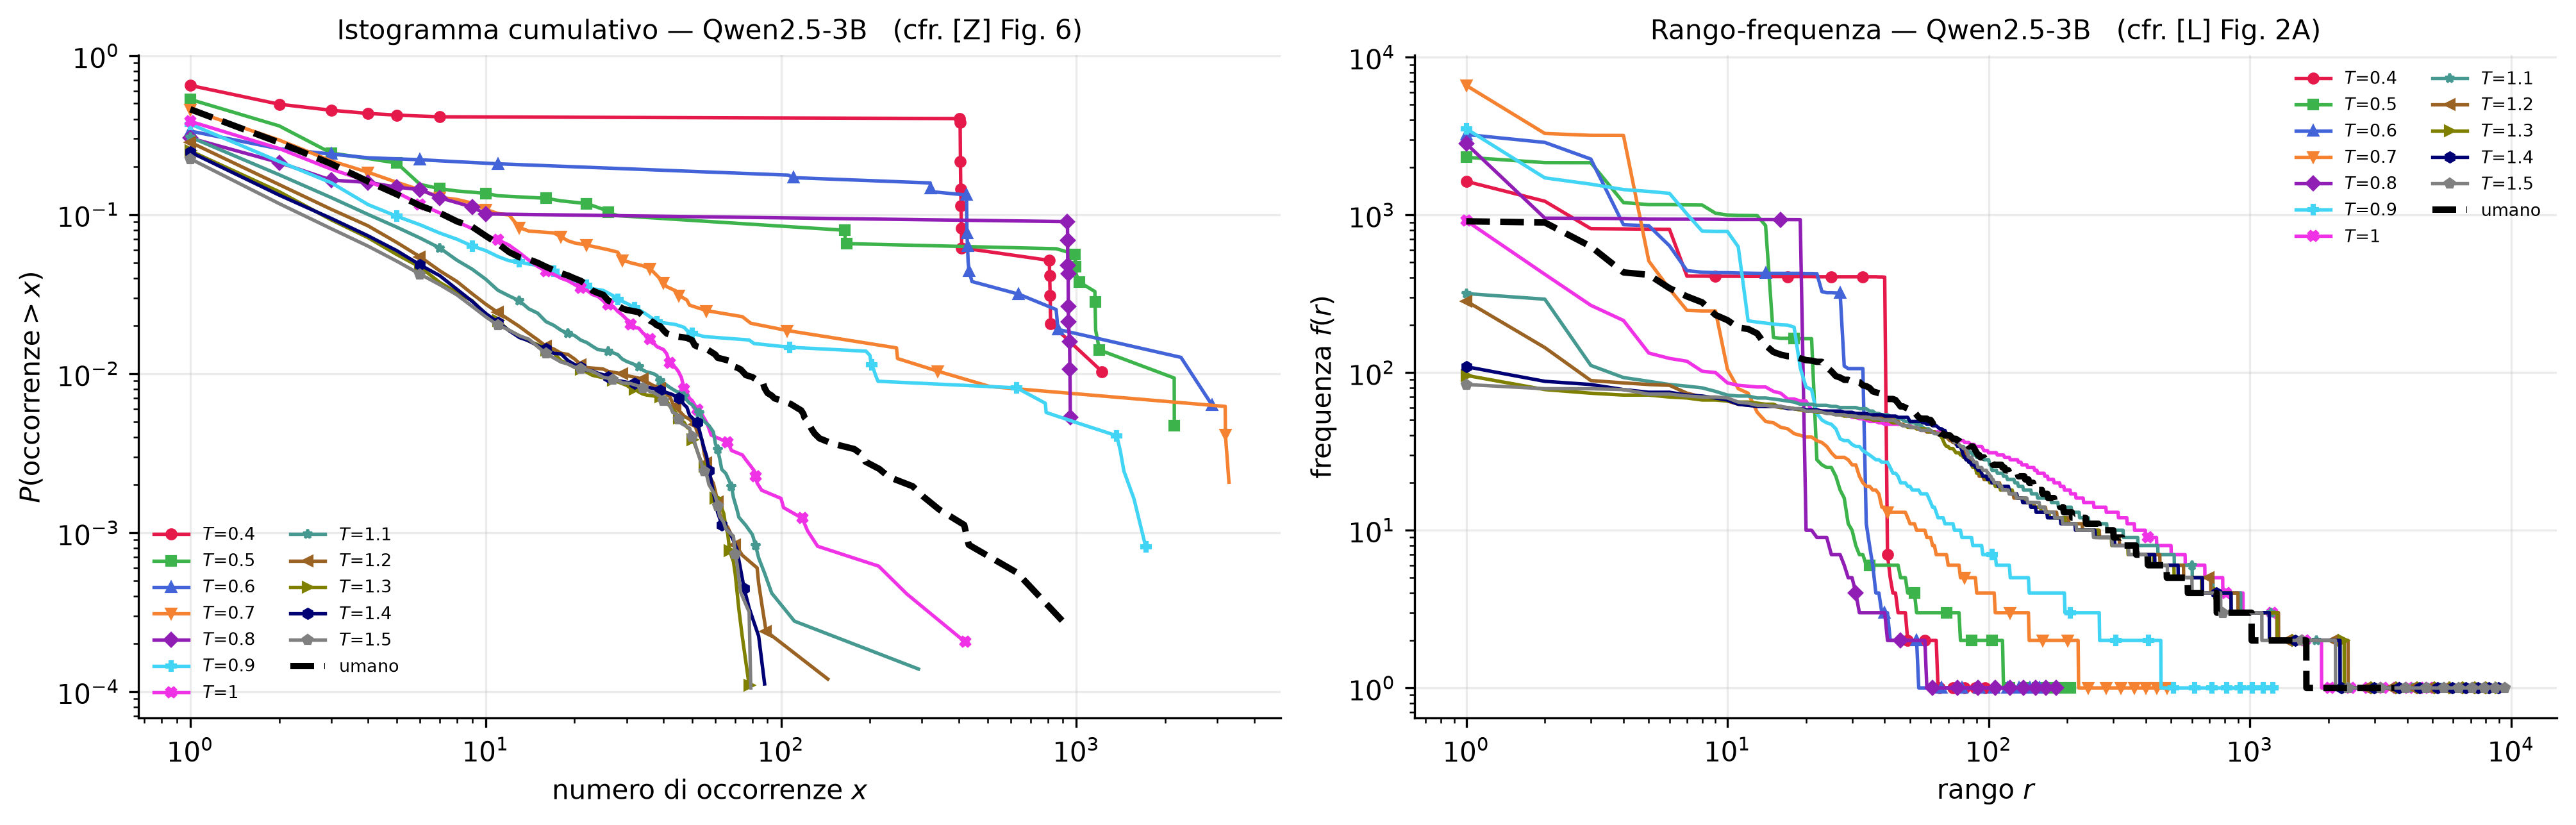
\includegraphics[width=\textwidth]{figure/cap4_zipf_cumulativo_Qwen25_3B.png}
  \caption{Istogrammi cumulativi delle frequenze dei token per il modello
  Qwen2.5-3B, una curva per temperatura. A bassa temperatura la curva è quasi
  verticale, perché pochi token coprono l'intero documento; ad alta temperatura
  è quasi orizzontale, perché quasi ogni token compare una volta sola. Solo
  nella regione intermedia la curva si avvicina alla retta che in coordinate
  bilogaritmiche corrisponde a una legge di potenza.}
  \label{fig:zipf-cum}
\end{figure}

L'esponente da solo non basta a descrivere questo comportamento, ed è la ragione
per cui nel §\ref{sec:zipf} è stato introdotto il MAPE: una curva può avere la
pendenza corretta e una curvatura marcata, e in tal caso l'esponente stimato non
descrive nulla. La Figura~\ref{fig:zipf-vs-T} riporta entrambe le quantità in
funzione della temperatura.

\begin{figure}[htbp]
  \centering
  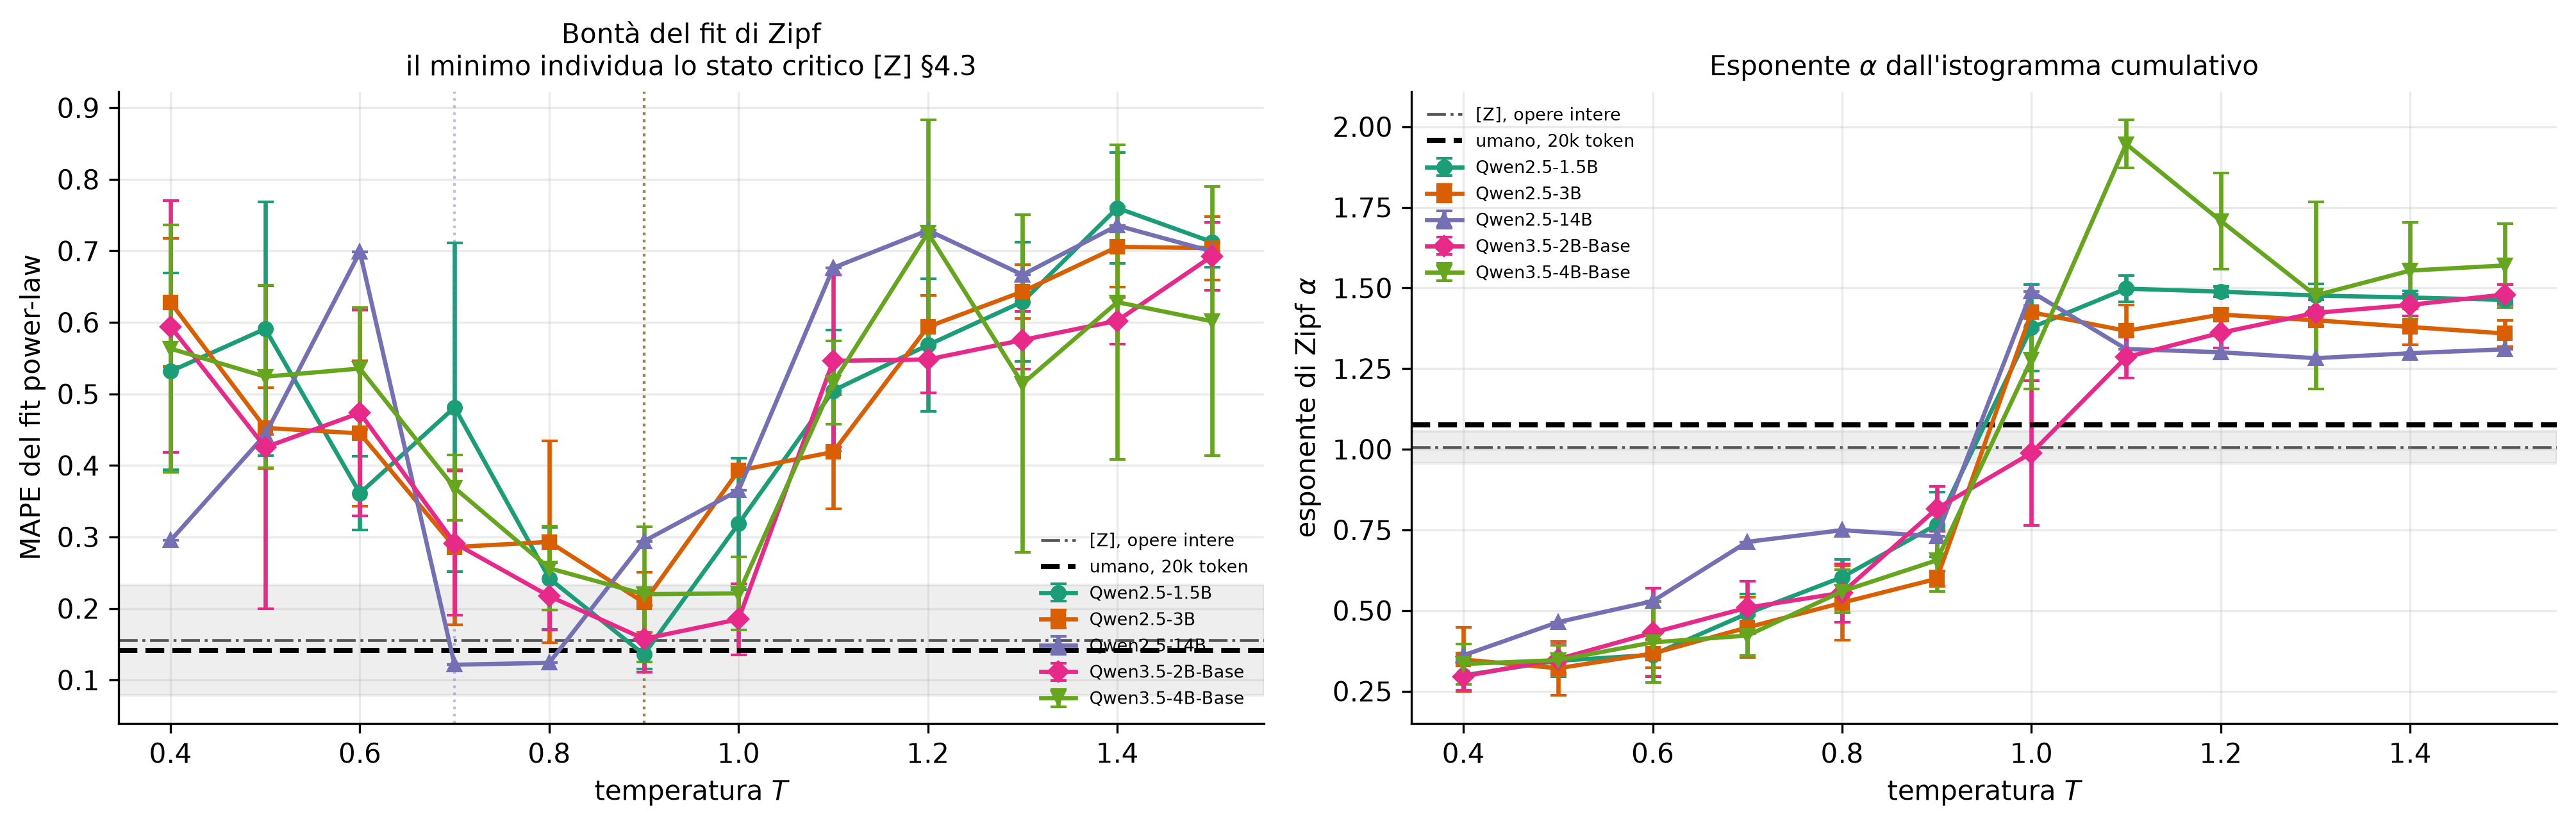
\includegraphics[width=\textwidth]{figure/cap4_zipf_vs_T.png}
  \caption{Bontà del fit e esponente della legge di Zipf in funzione della
  temperatura, per tutti e cinque i modelli. La banda grigia è il valore
  pubblicato su testi letterari interi, la linea nera tratteggiata la baseline
  umana misurata alla lunghezza di lavoro.}
  \label{fig:zipf-vs-T}
\end{figure}

Il MAPE ha un minimo pronunciato, che cade a $T = 0.9$ per quattro modelli su
cinque e a $T = 0.7$ per il modello da 14 miliardi di parametri. È il
risultato centrale della sezione: esiste una temperatura alla quale la
distribuzione delle frequenze del testo generato è più vicina a una legge di
potenza, e ai due lati di essa l'aderenza peggiora rapidamente.

Al minimo il MAPE del modello esemplare vale $0.208$. I due termini di
riferimento sono la baseline umana misurata alla stessa lunghezza, che vale
$0.141$, e il valore $0.156 \pm 0.077$ che~\cite{mikhaylovskiy2025zipf} riporta
su un corpus di sei opere letterarie in cinque lingue. Che i due riferimenti
umani cadano tanto vicini è una verifica indipendente della taratura della
baseline: sono ottenuti con tokenizzatori diversi, su testi diversi e di
lunghezza diversa, e la deriva documentata nella
Figura~\ref{fig:dimensione-finita} non rendeva scontato l'accordo.

Il valore del modello va letto contro tre metri diversi, e il giudizio che se ne
ricava non è lo stesso. Rispetto al modello stesso, $0.208$ è un risultato
netto: alle due estremità dell'intervallo lo stesso modello dà $0.628$ e
$0.704$, cioè un errore di fit tre volte più grande. Rispetto al testo umano è
invece una mezza vittoria: $0.208$ è circa una volta e mezza $0.141$, e resta
dentro la banda pubblicata solo perché quella banda è larga, sfiorandone il
margine superiore $0.233$. Rispetto agli altri modelli, infine, è un risultato
mediocre. La Tabella~\ref{tab:mape-minimi} riporta i cinque minimi: due modelli
scendono sotto il valore umano e un terzo vi si accosta, con $0.158$ contro
$0.141$, mentre il modello esemplare e il Qwen3.5-4B restano sopra.

\begin{table}[htbp]
\centering
\small
\begin{tabular}{@{}lrr@{}}
\toprule
Modello & $T$ del minimo & MAPE al minimo \\
\midrule
Qwen2.5-14B      & 0.7 & 0.121 \\
Qwen2.5-1.5B     & 0.9 & 0.136 \\
Qwen3.5-2B-Base  & 0.9 & 0.158 \\
Qwen2.5-3B       & 0.9 & 0.208 \\
Qwen3.5-4B-Base  & 0.9 & 0.220 \\
\midrule
testo umano      & --- & 0.141 \\
\bottomrule
\end{tabular}
\caption{Valore minimo del MAPE e temperatura alla quale viene raggiunto, per
ciascun modello, con la baseline umana misurata alla stessa lunghezza. Il
minimo esiste per tutti e cinque, ma solo tre modelli lo portano al livello del
testo umano o sotto. La riga del Qwen2.5-14B è ricavata da un solo campione per
temperatura e va letta con la cautela discussa nel testo.}
\label{tab:mape-minimi}
\end{table}

La prima riga della tabella richiede una precauzione. Il Qwen2.5-14B è l'unico
modello con un solo campione per temperatura, contro i tre o cinque degli altri,
e la sua curva del MAPE non è regolare da nessuno dei due lati del minimo: vale
$0.295$ a $T = 0.4$, sale a $0.698$ a $T = 0.6$ e scende a $0.121$ a $T = 0.7$,
cioè peggiora di un fattore due e migliora di un fattore sei in due passi
consecutivi. Negli altri quattro modelli la dispersione fra campioni alla stessa
temperatura va da $0.046$ a $0.230$ attorno a $T = 0.7$, mentre la distanza fra
il minimo del 14B e il suo valore a $T = 0.9$ vale $0.173$: sta dentro
quell'intervallo. Con una sola realizzazione la posizione del minimo non è
risolvibile, e il valore $T = 0.7$ va letto come compatibile con il $T = 0.9$
degli altri quattro anziché come uno spostamento reale. La stessa cautela vale
per la profondità: $0.121$ è il minimo più basso dei cinque ed è anche il meno
affidabile, mentre il $0.136$ del Qwen2.5-1.5B poggia su cinque campioni con
dispersione $0.020$ ed è l'unico caso in cui il primato sul testo umano è
sostenuto da repliche.

La posizione del minimo va confrontata con quella riportata nella fonte.
In~\cite{mikhaylovskiy2025zipf} il minimo del MAPE cade fra $t = 1.0$ e
$t = 1.2$ per tutti i modelli tranne i Llama più grandi, mentre qui cade a
$T = 0.9$ per quattro modelli su cinque. Lo scarto è nella direzione prevista
dall'effetto del prompt descritto nel §\ref{sec:protocollo}, che abbassa
l'errore del fit soprattutto alle basse temperature e sposta quindi il minimo
verso sinistra.

Ne segue una distinzione che vale per tutto il seguito. L'esistenza
di una temperatura ottimale è un fatto generale, comune a tutti e cinque i
modelli; la qualità dell'ottimo, cioè quanto il testo generato in quel punto
somigli davvero a un testo umano, varia da modello a modello e non è garantita.
Il modello scelto come esemplare non è fra quelli che ci riescono, e i grafici
del corpo del capitolo vanno letti tenendolo presente.

L'esponente $\alpha$ racconta la stessa storia da un'altra angolazione. Per il
modello esemplare passa da $0.35$ a $T = 0.4$, valore che corrisponde a una
distribuzione dominata da pochissimi tipi, a $1.36$ a $T = 1.5$, dove più di tre
quarti dei tipi compaiono una volta sola.\footnote{Un tipo che compare una sola
volta nel testo si dice \emph{hapax}. Gli hapax sono normalmente la maggioranza
dei tipi ma una piccola parte delle occorrenze: nella baseline umana usata qui
sono il $54\%$ dei tipi e il $10\%$ dei token, mentre a $T = 1.5$ il modello
esemplare arriva al $77\%$ dei tipi e al $37\%$ dei token.} La transizione non è
graduale: fra $T = 0.9$ e $T = 1.0$ l'esponente salta da $0.60$ a $1.43$,
attraversando in un solo passo il valore umano $1.076$, per poi assestarsi
attorno a $1.4$ senza più avvicinarvisi.

% ---------------------------------------------------------------------
\section{Legge di Heaps e descrittore \texorpdfstring{$R$}{R}}
\label{sec:heaps-risultati}

Le curve di crescita del vocabolario rendono immediatamente evidente perché il
§\ref{sec:heaps} abbia dovuto introdurre un descrittore alternativo all'esponente di
Heaps.

\begin{figure}[htbp]
  \centering
  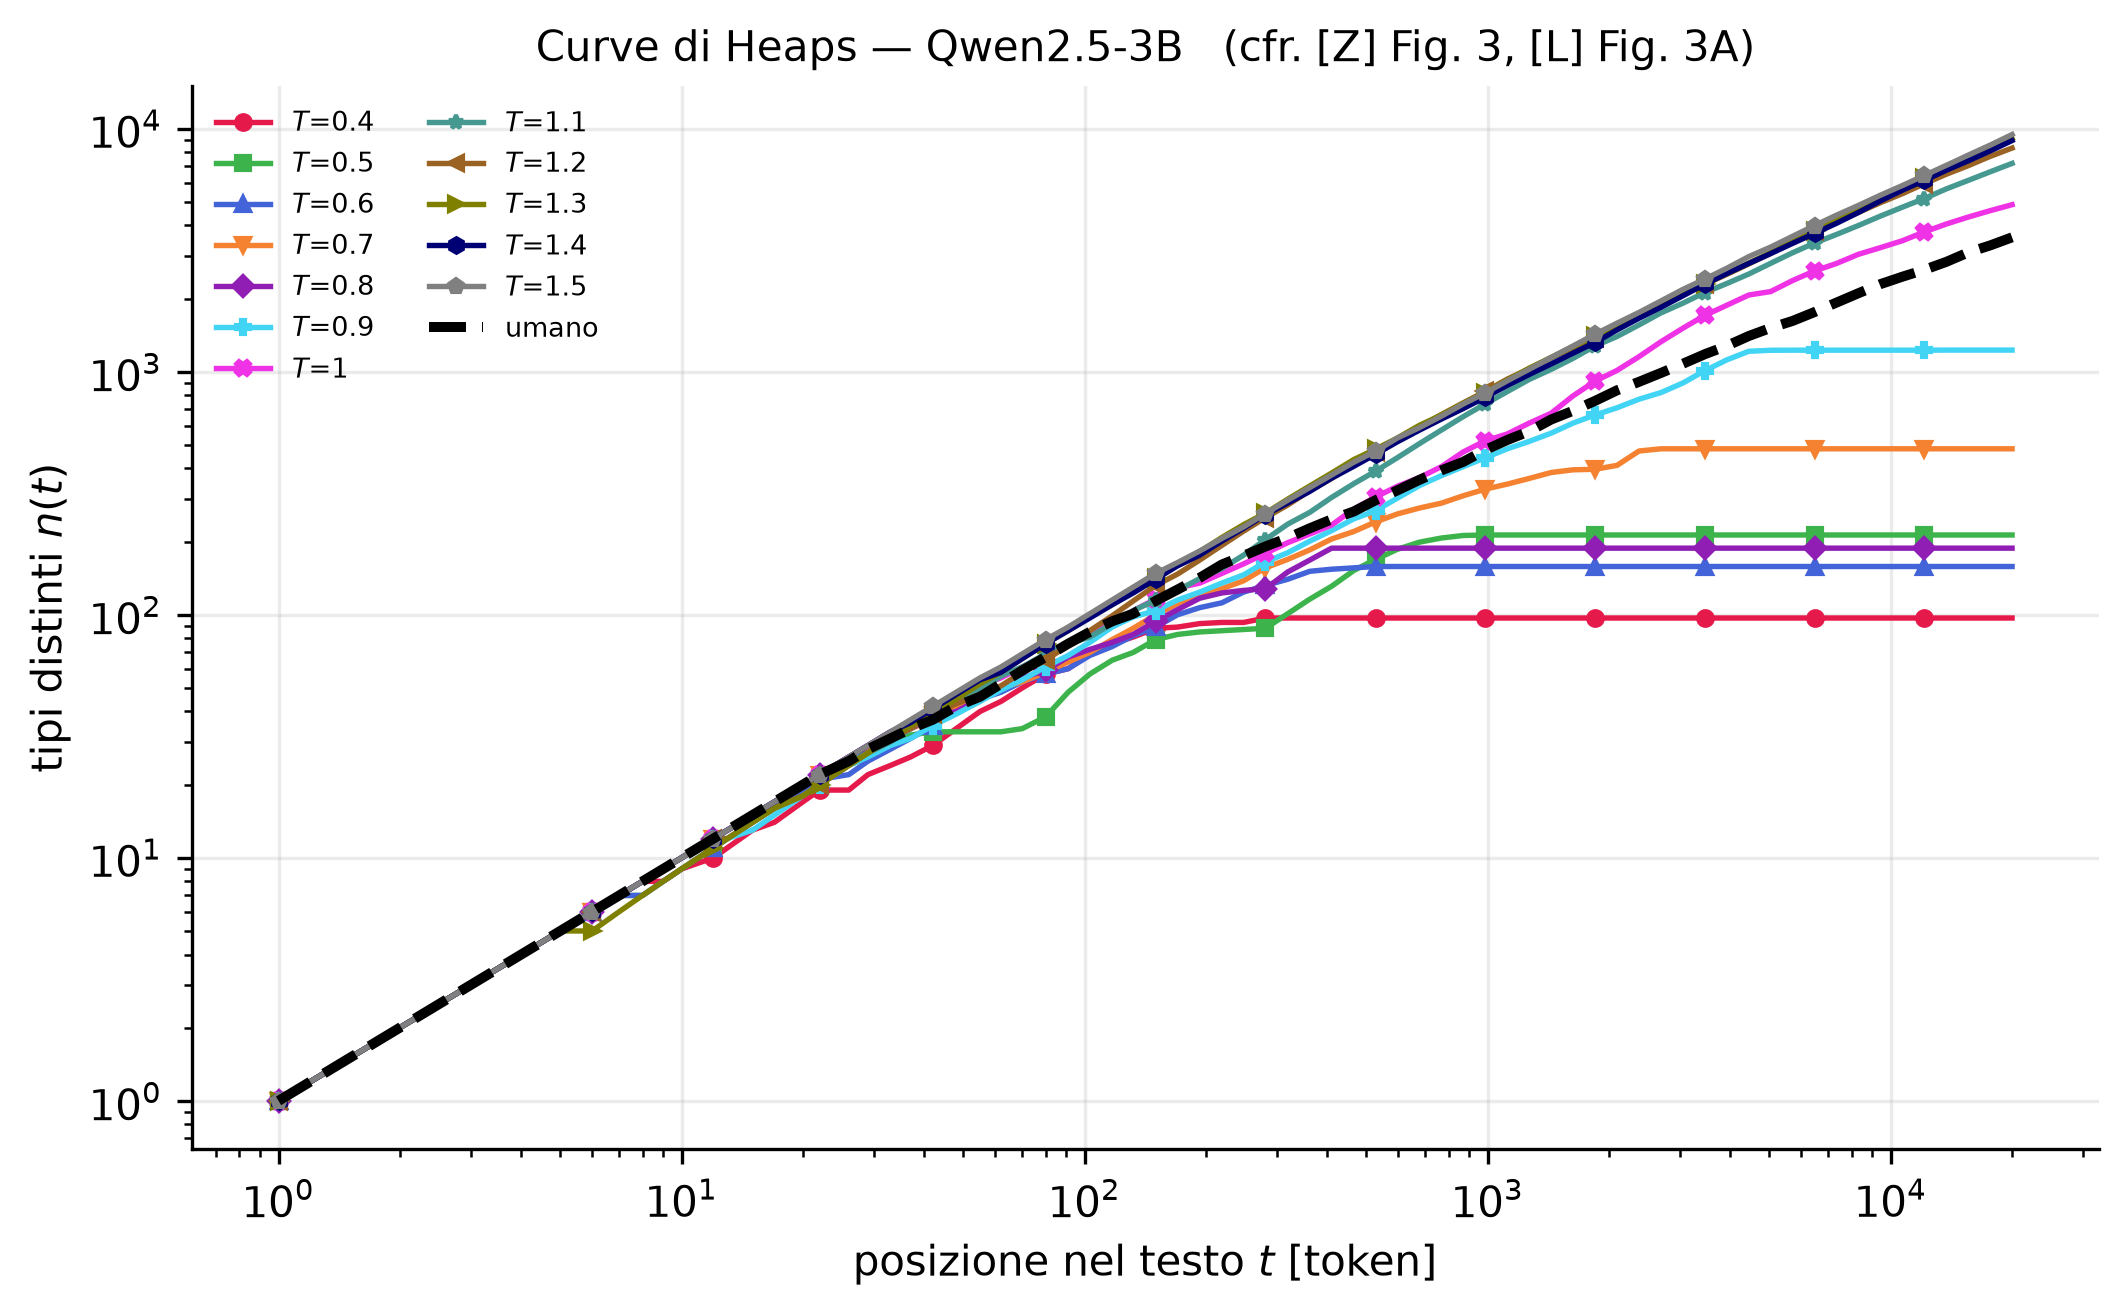
\includegraphics[width=0.86\textwidth]{figure/cap4_heaps_curve_Qwen25_3B.png}
  \caption{Crescita del vocabolario per il modello Qwen2.5-3B. Alle temperature
  basse la curva si appiattisce dopo poche migliaia di token: il modello ha
  smesso di produrre tipi nuovi. Alle temperature alte cresce quasi linearmente.
  In nessuno dei due casi la curva è una legge di potenza, e stimarne
  l'esponente restituisce un numero privo di contenuto.}
  \label{fig:heaps-curve}
\end{figure}

La Figura~\ref{fig:heaps-R} riporta il descrittore $R$, l'esponente $\gamma_H$
e il rapporto fra tipi e occorrenze in funzione della temperatura. I tre
andamenti sono concordi: per il modello esemplare $\gamma_H$ passa da $0.001$
a $T = 0.4$, dove la curva è piatta e il vocabolario non cresce affatto, a
$0.806$ a $T = 1.5$, attraversando il valore umano $0.668$ poco sopra $T =
0.9$. Il descrittore $R$ passa da $0.003$ a $0.688$ e incrocia il valore umano
$0.507$ attorno a $T = 1.05$.

Il terzo pannello riporta la quantità più elementare delle tre, il rapporto fra
il numero di tipi distinti e il numero di occorrenze, e serve da controllo sulle
altre due. A differenza di $\gamma_H$ e di $R$ non richiede alcun fit né alcuna
partizione del documento, quindi non può essere alterato da un modello mal
specificato: se le tre curve concordano, l'andamento non è un artefatto della
procedura di stima. Per il modello esemplare passa da $0.007$ a $T = 0.4$ a
$0.474$ a $T = 1.5$, e attraversa il valore umano $0.179$ fra $T = 0.9$ e
$T = 1.0$, cioè nello stesso punto delle altre due misure. Il pannello mostra
però anche in che senso l'accordo con il testo umano sia solo locale: sopra
$T = 1.1$ il rapporto supera il doppio del valore umano e continua a crescere,
mentre $\gamma_H$ resta stabile attorno a $0.8$. Le due misure smettono di dire
la stessa cosa non appena il vocabolario si allarga oltre quello di un romanzo.

\begin{figure}[htbp]
  \centering
  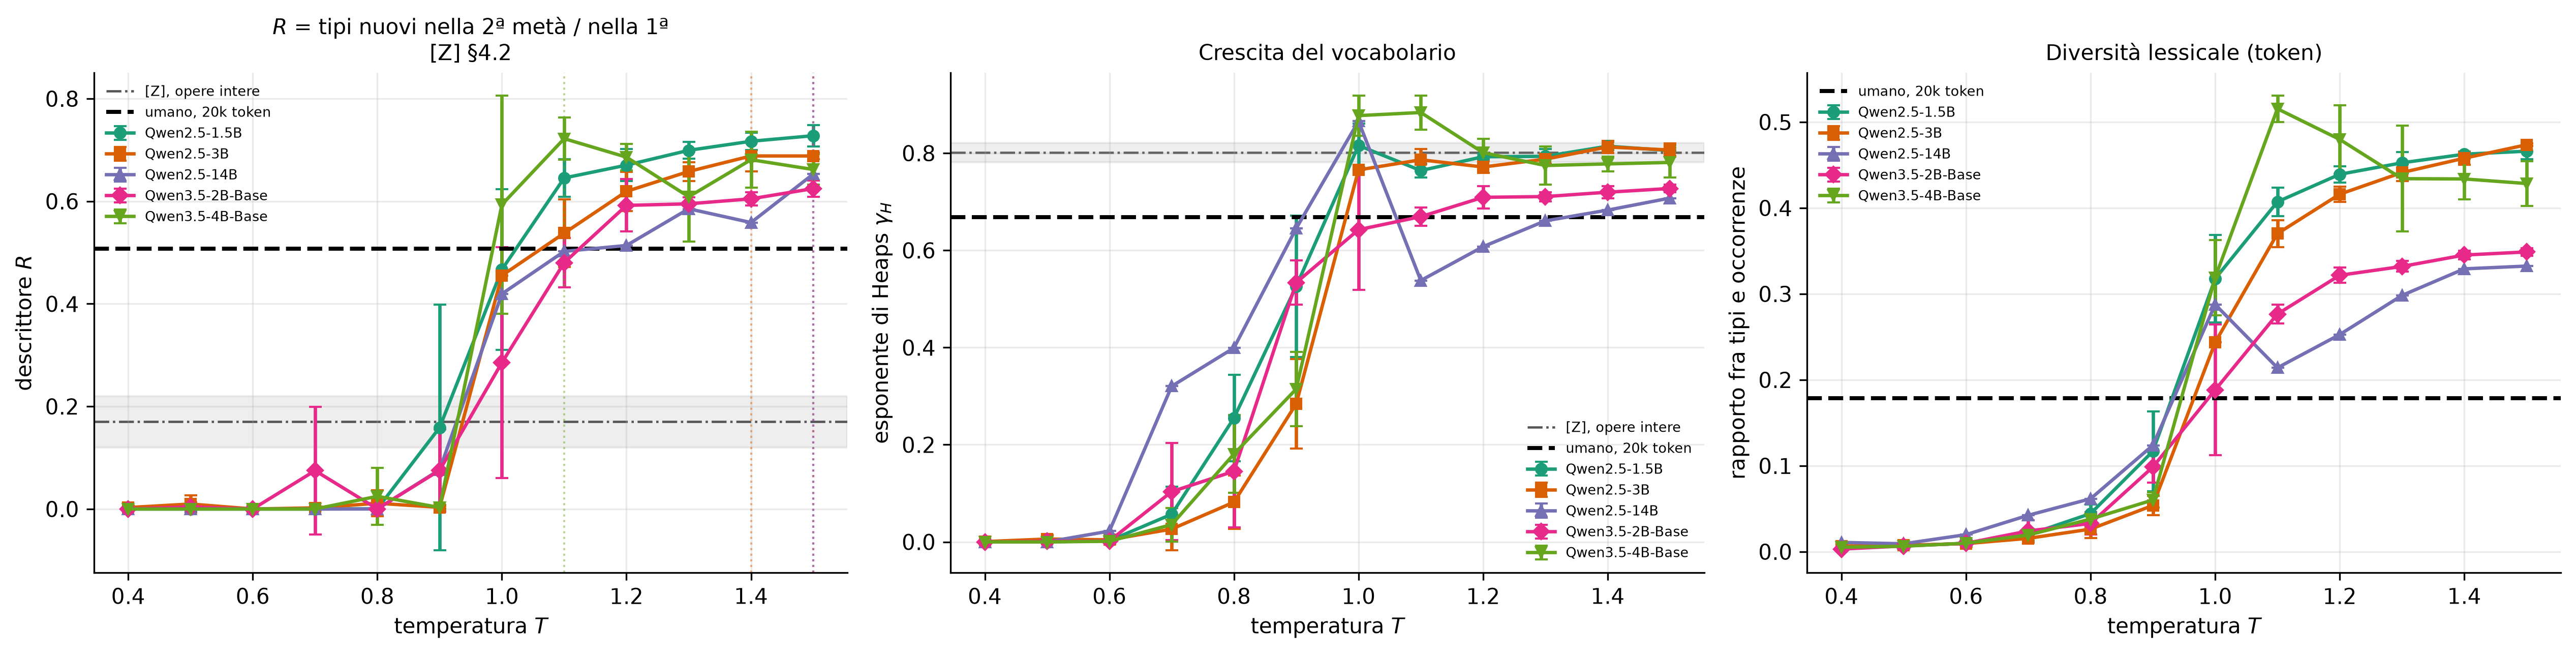
\includegraphics[width=\textwidth]{figure/cap4_heaps_R_vs_T.png}
  \caption{Descrittore $R$, esponente di Heaps e rapporto fra tipi e occorrenze
  in funzione della temperatura. La banda grigia riporta i valori pubblicati su
  opere intere, che per le ragioni discusse nel §\ref{sec:scelte} non sono un
  termine di confronto diretto.}
  \label{fig:heaps-R}
\end{figure}

% ---------------------------------------------------------------------
\section{Correlazioni a lungo raggio}
\label{sec:dfa-risultati}

Ogni documento viene convertito nella successione numerica definita nel
§\ref{sec:dfa}: ogni carattere è sostituito dal proprio rango di frequenza nel
documento, $1$ al più frequente, $2$ al secondo, e così via. È su quella
successione che si misura l'esponente della fluttuazione. Il detrending è
quadratico: il §\ref{sec:robustezza} documenta il confronto con quello lineare e
la ragione della scelta, cioè che alle basse temperature i documenti non sono
stazionari e un polinomio di primo grado non assorbe la deriva della
composizione dei caratteri. Il primo controllo riguarda il null model: la stessa
analisi condotta sui documenti rimescolati deve restituire un esponente pari a
$1/2$.


La Figura~\ref{fig:dfa} riporta le curve di fluttuazione e l'esponente in
funzione della temperatura. L'esponente ha un massimo a $T = 1.0$, dove vale
$0.719$ in media su tutti i modelli, superiore al valore umano di $0.579$;
decresce poi verso $0.53$ alle temperature più alte, avvicinandosi al valore del
rimescolamento senza raggiungerlo.

\begin{figure}[htbp]
  \centering
  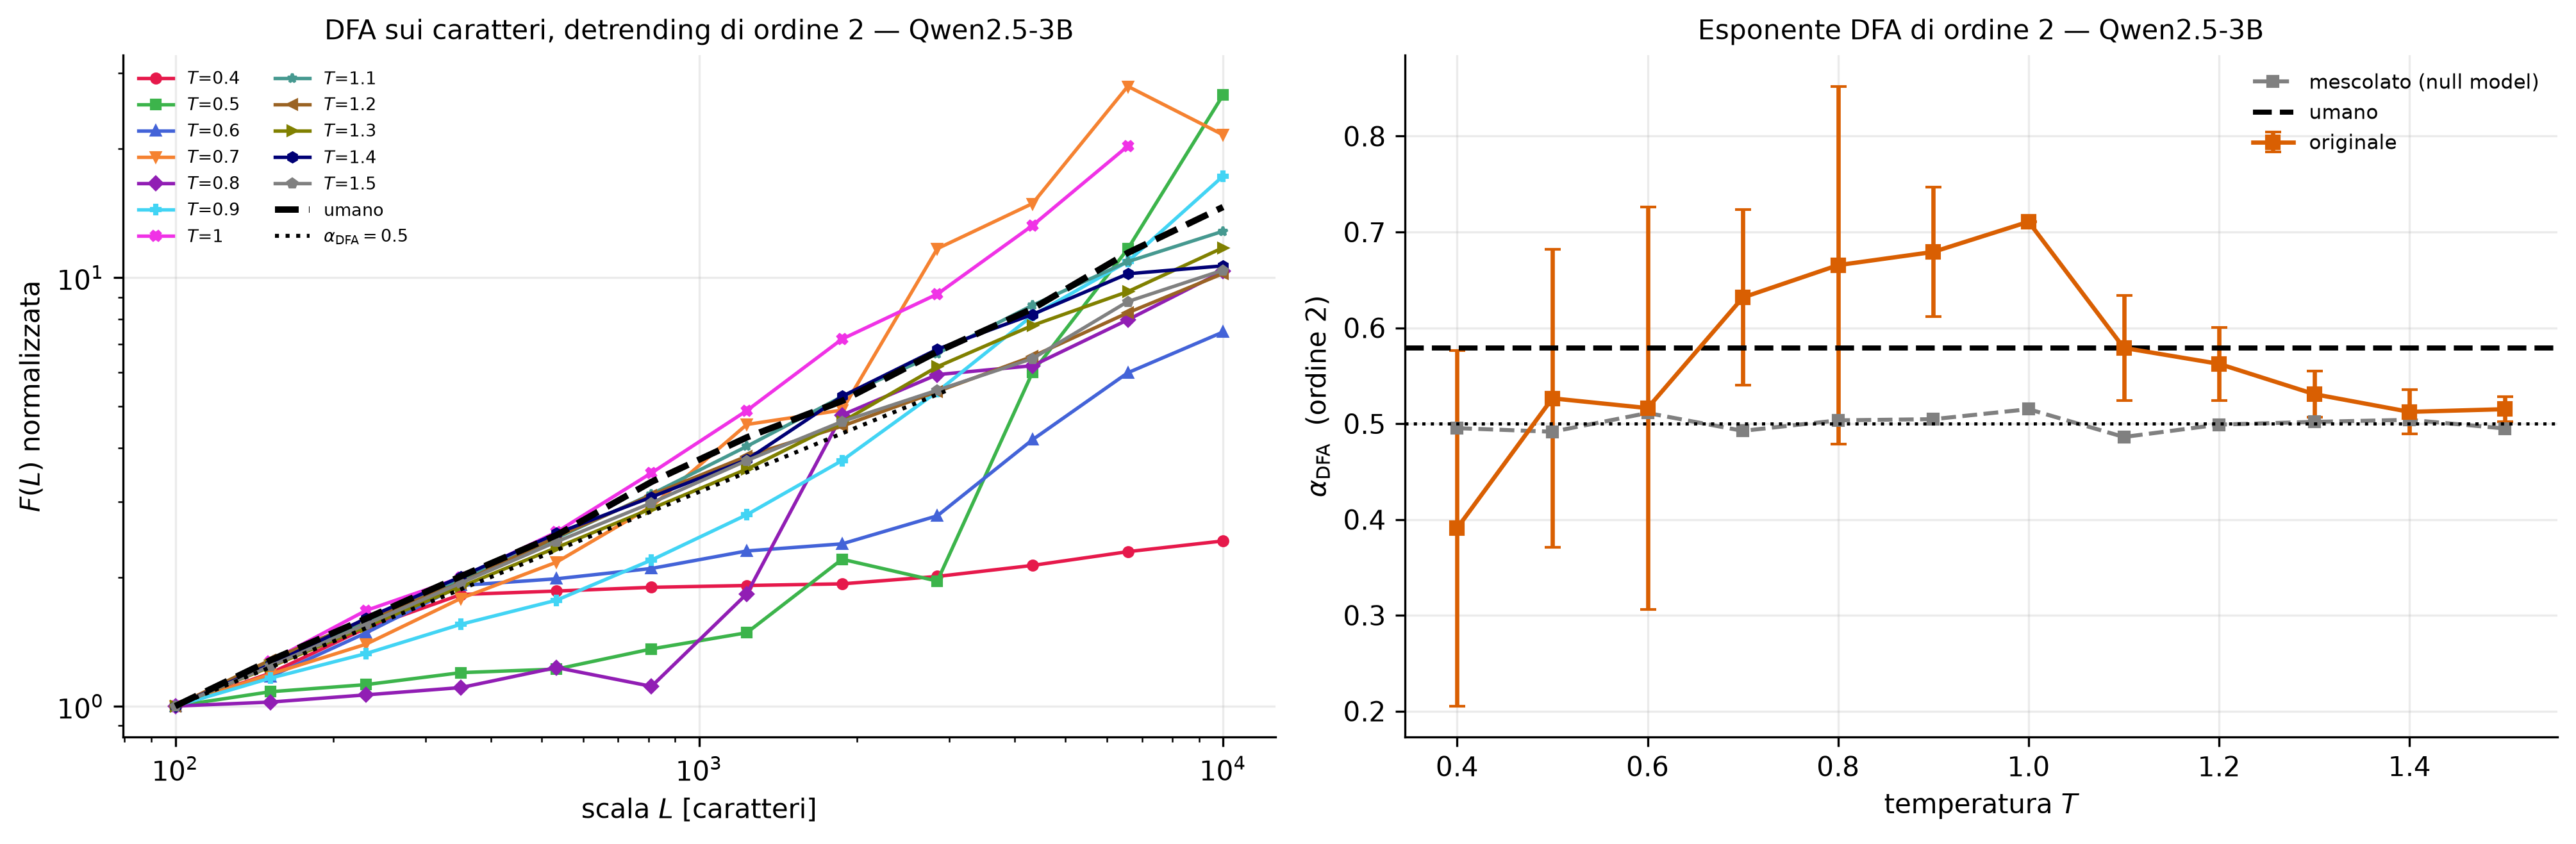
\includegraphics[width=\textwidth]{figure/cap4_dfa_Qwen25_3B_o2.png}
  \caption{Fluttuazione detrendizzata per il modello Qwen2.5-3B, con detrending
  quadratico. A sinistra $F(s)$ in funzione della scala, una curva per
  temperatura, con la pendenza di riferimento $\alpha_{\mathrm{DFA}} = 1/2$; a
  destra l'esponente in funzione della temperatura, con il null model
  rimescolato e la baseline umana.}
  \label{fig:dfa}
\end{figure}

\paragraph{La dispersione è il vero segnale.}
Il valore medio dell'esponente nasconde il fenomeno più informativo, ed è un
fenomeno già osservato: sulle reti LSTM~\cite{lippi2019} riporta che le stime
sui singoli campioni sono molto disperse attorno a $T = 0.5$ e strettamente
raccolte attorno alla media a $T = 1.0$. Gli stessi dati mostrano qui lo stesso
comportamento su architetture transformer. La deviazione standard fra documenti
passa da $0.219$ a $T = 0.4$ a $0.022$ a $T = 1.4$: alle basse temperature la
stima è dieci volte più dispersa. A $T = 0.4$ i cinque documenti del modello
esemplare danno esponenti compresi fra $0.16$ e $0.66$, cioè coprono
l'intervallo fra la saturazione e il valore umano; sull'insieme dei cinque
modelli l'escursione va da $0.07$ a $0.89$.

Questo comportamento è coerente con il caso limite discusso nel
§\ref{sec:ponte}. Quando il testo entra in un ciclo di ripetizione, il profilo
cumulato oscilla invece di allontanarsi dall'origine e la fluttuazione satura:
l'esponente crolla. Il crollo dipende però dalla lunghezza del ciclo rispetto
alle scale analizzate, che varia da documento a documento, e non tutti i testi
ripetitivi lo manifestano.

I dati permettono di precisare la relazione, che è a senso unico. Tutti e
diciannove i documenti con $\alpha_{\mathrm{DFA}} < 0.3$ si trovano a
$T \le 0.6$ e hanno una quota media di 8-grammi ripetuti pari a $0.984$: un
esponente collassato implica dunque ripetizione conclamata. Il viceversa non
vale: fra gli 82 documenti con quota di 8-grammi ripetuti superiore a $0.9$,
soltanto 33 hanno un esponente inferiore a $1/2$, e la correlazione di rango fra
le due quantità non è significativa
($\rho = +0.03$, $p = 0.61$). La ripetizione è quindi condizione necessaria ma
non sufficiente al collasso dell'esponente.

Ne segue una conseguenza metodologica. Alle basse temperature
$\alpha_{\mathrm{DFA}}$ non è un indicatore affidabile di correlazione a lungo
raggio, né lo è il suo valore medio; è la sua dispersione a segnalare il regime.
Il controllo sull'ordine del detrending riportato nel §\ref{sec:robustezza}
punta nella stessa direzione, poiché lo scarto fra i due ordini è massimo
proprio nell'intervallo $T \in [0.5, 0.8]$ e trascurabile altrove.

% ---------------------------------------------------------------------
\section{Entropia, divergenza dal testo umano e plagio}
\label{sec:entropia-risultati}

Le sezioni precedenti confrontano il testo generato con quello umano una misura
alla volta. La divergenza di Kullback--Leibler introdotta nel
§\ref{sec:crossparsing} permette invece un confronto diretto fra i due testi,
senza passare per un descrittore intermedio, ed è per questa ragione il criterio
più stringente del capitolo: non dipende da soglie teoriche né dalla scelta di
quale proprietà misurare.


La divergenza ha un minimo netto, che cade a $T = 0.9$ per quattro modelli su
cinque e a $T = 1.0$ per Qwen3.5-4B-Base. Nessuna delle \num{242} stime risulta
negativa, il che conferma sui dati reali la proprietà dello stimatore verificata
nel §\ref{sec:validazione}.

Il valore al minimo varia molto fra i modelli: $0.096$ bit per carattere per il
modello da 14 miliardi di parametri, $0.232$ e $0.245$ per i due Qwen3.5,
$0.321$ per il modello da 1.5 miliardi e $0.914$ per quello da 3 miliardi. La
posizione del minimo è dunque comune, la sua profondità no: fra il modello che
si avvicina di più al testo umano e quello che ci riesce meno corre quasi un
fattore dieci. La profondità non segue però la dimensione. La correlazione di
rango con il numero di parametri vale $\rho = -0.50$ con $p = 0.39$ su cinque
modelli, e il valore peggiore appartiene al modello da 3 miliardi anziché al più
piccolo: quanto un modello si avvicini al testo umano nel proprio punto migliore
è una proprietà del singolo modello, non della sua scala, almeno con la potenza
statistica qui disponibile. Vale inoltre la cautela imposta dal
§\ref{sec:robustezza}, poiché il modello da 14 miliardi dispone di un solo
campione per temperatura e il suo valore non è corredato da una stima della
dispersione.

L'entropia stimata per compressione mostra la transizione in modo ancora più
brusco. Per il modello esemplare la mediana vale $0.001$ bit per carattere
fino a $T = 0.8$, perché il testo ripetitivo è essenzialmente incomprimibile
oltre la prima occorrenza del ciclo e non trasporta informazione; sale poi a
$0.332$ in media a $T = 0.9$ e supera $4$ da $T = 1.0$ in poi, contro i $2.23$
del testo umano. Fra $T = 0.6$ e $T = 0.9$ la media si stacca dalla mediana
perché un documento per temperatura esce dal ciclo prima degli altri, e il
valore isolato di $5.77$ che il modello esemplare raggiunge a $T = 1.0$
proviene dall'unico documento sopravvissuto a quella temperatura: è la stessa
dispersione descritta nel §\ref{sec:dfa-risultati}, e conferma che nel regime
periodico il valore medio non descrive alcun documento. Il passaggio dal
regime a entropia trascurabile a quello a entropia superiore a quella umana si
consuma comunque entro due passi di temperatura.

% ---------------------------------------------------------------------
\section{Struttura misurata per compressione}
\label{sec:compressione-risultati}

Le misure basate su compressione del §\ref{sec:compressione} non richiedono di
scegliere un'unità di analisi né di stimare un esponente: operano direttamente
sui byte del testo. Costituiscono quindi un controllo indipendente da tutte le
scelte metodologiche discusse finora.

\begin{figure}[htbp]
  \centering
  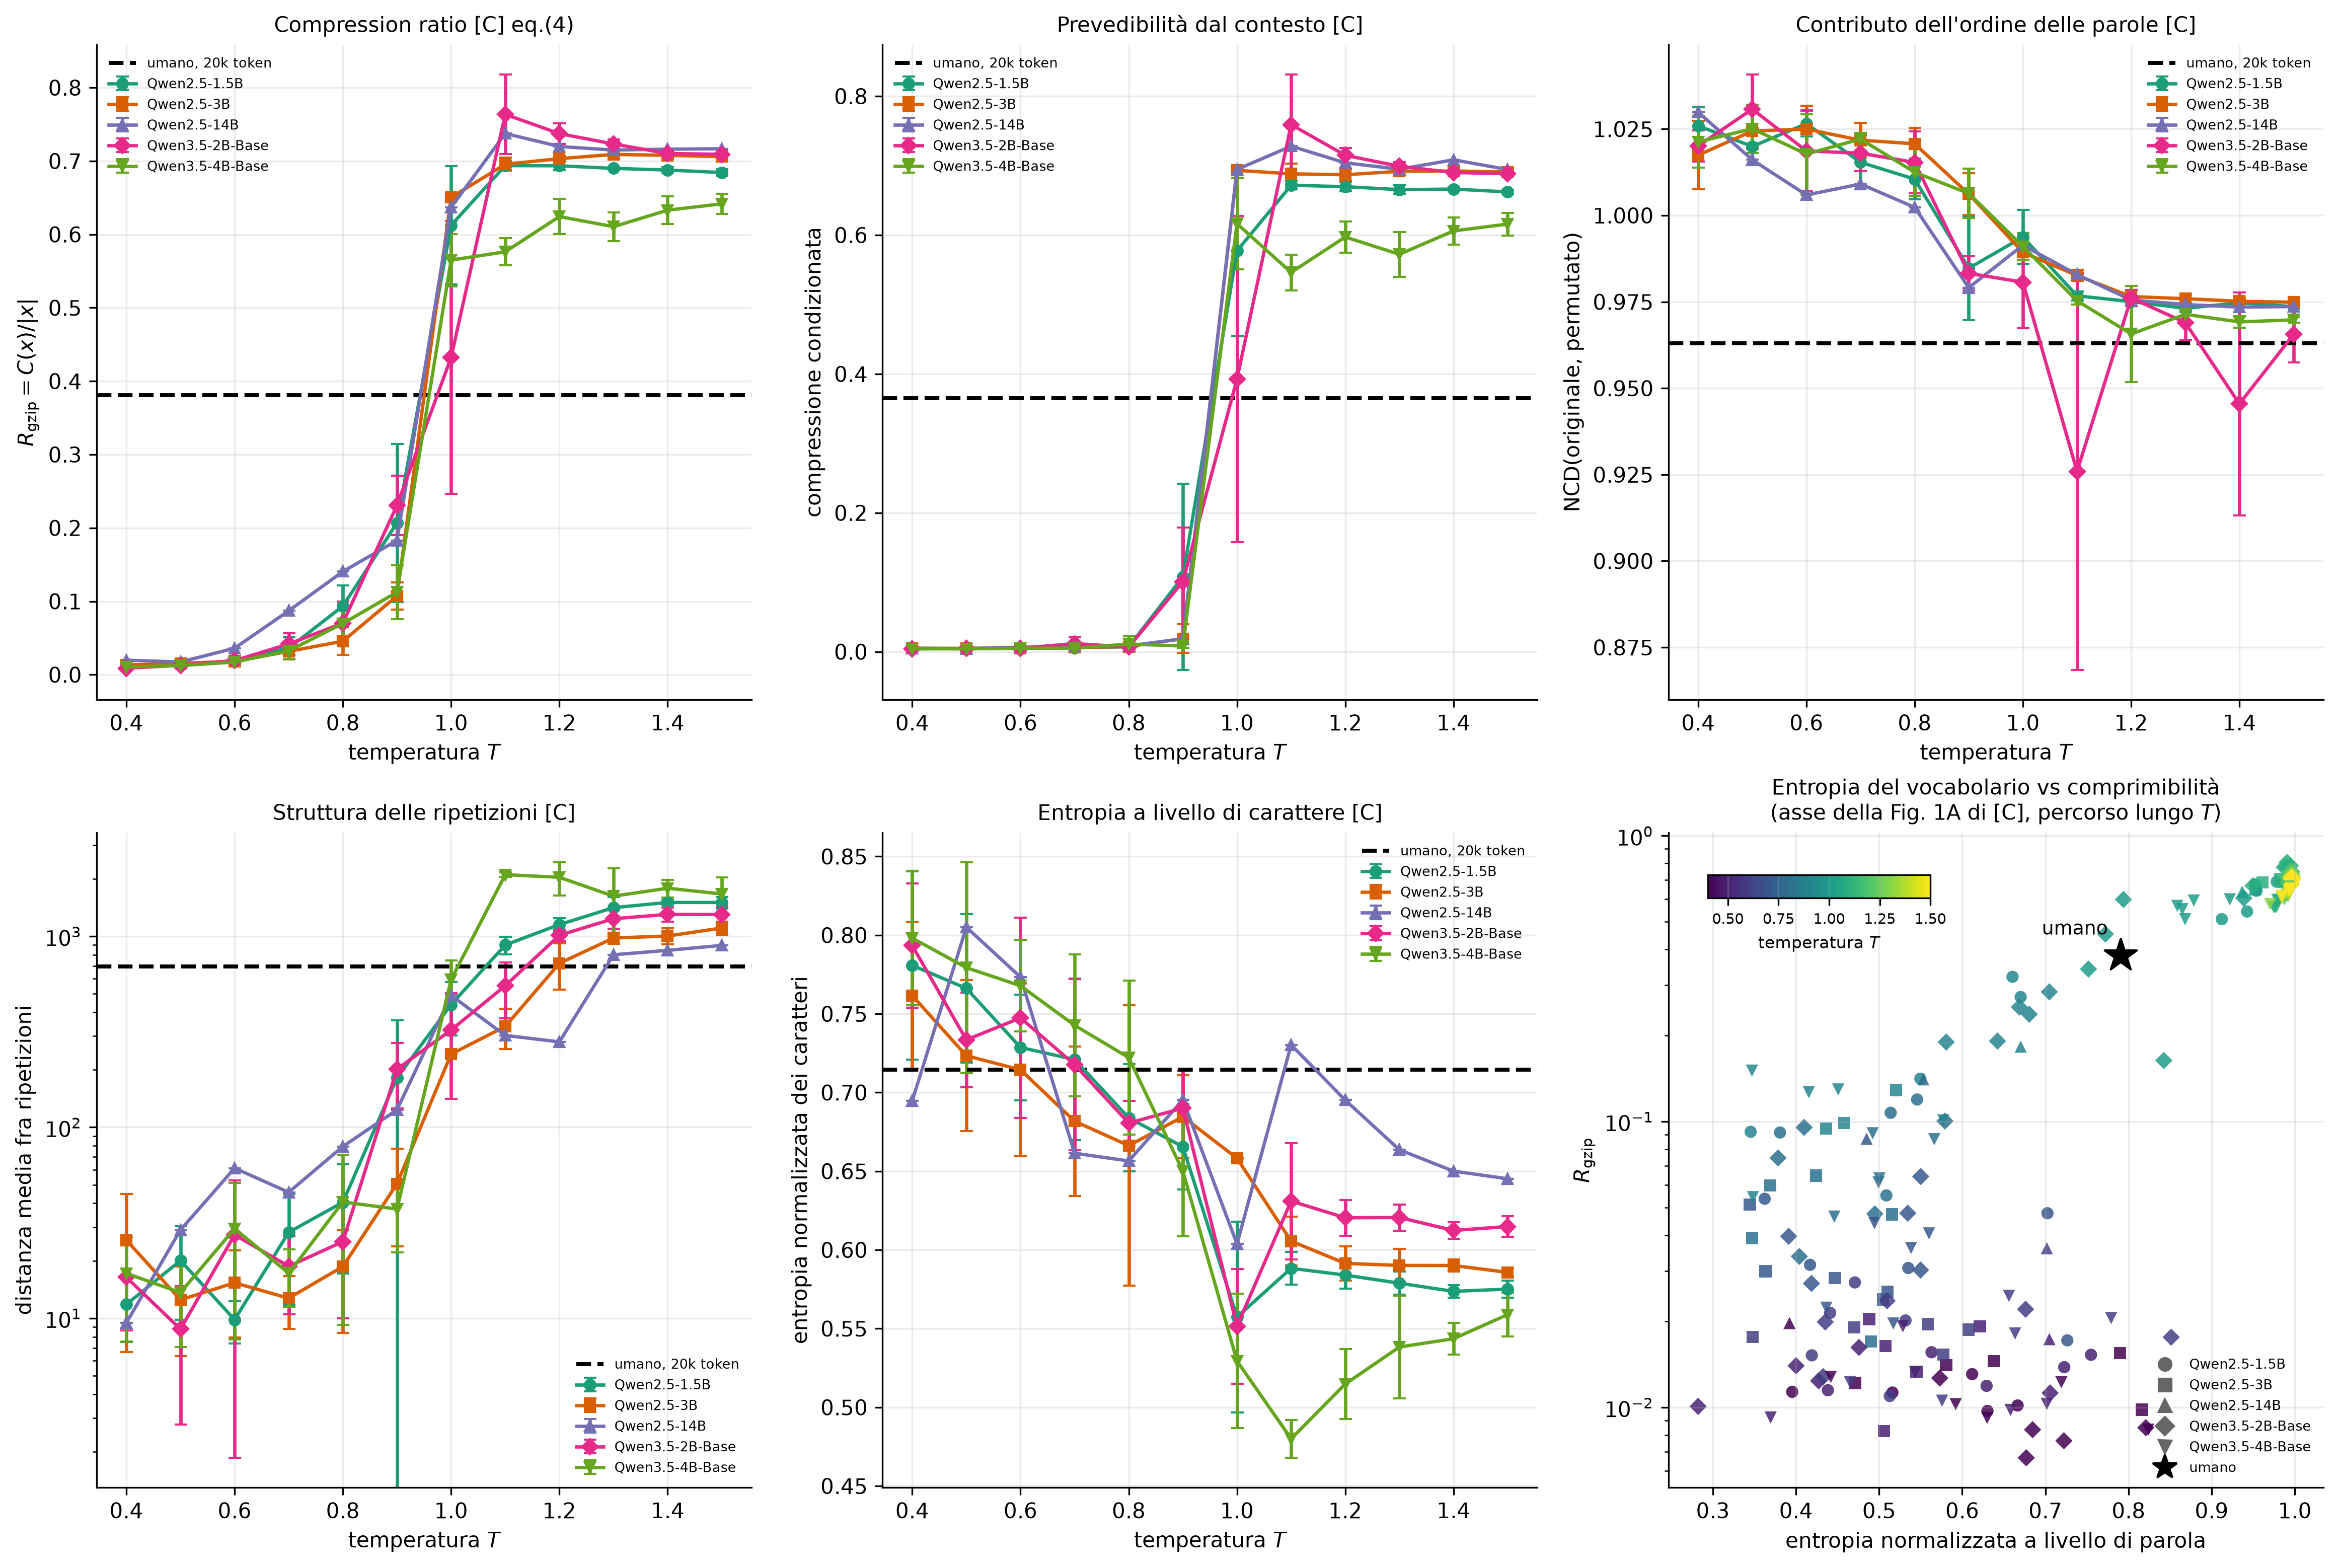
\includegraphics[width=\textwidth]{figure/cap4_compressione.png}
  \caption{Sei misure basate su compressione. Le prime cinque sono riportate in
  funzione della temperatura; l'ultima, in basso a destra, riporta il rapporto
  di compressione contro
  l'entropia normalizzata a livello di parola: è il piano della Figura~1A
  di~\cite{hadad2026}, percorso qui facendo variare la temperatura, con il testo
  umano segnato da una stella. In quel pannello il colore codifica la
  temperatura e la forma del marcatore il modello, e la scala verticale è
  logaritmica.}
  \label{fig:compressione}
\end{figure}

Il rapporto di compressione è la misura che separa i regimi in modo più netto di
tutte le altre. Per il modello esemplare passa da $0.013$ a $T = 0.4$ a $0.107$
a $T = 0.9$ e a $0.650$ a $T = 1.0$: un fattore cinquanta fra i due estremi, con
un salto di un fattore sei concentrato in un singolo passo di temperatura. Il
valore umano è $0.381$, e viene attraversato fra $T = 0.9$ e $T = 1.0$ come
tutte le altre misure del capitolo.

Il lavoro di~\cite{hadad2026} riporta che il testo generato è più regolare e
più comprimibile di quello umano, mentre qui il rapporto di compressione
supera il valore umano sopra $T = 1.0$. Le due osservazioni non sono in
contrasto, perché descrivono regioni diverse dello stesso asse: sotto la
transizione il testo generato è molto più comprimibile del testo umano,
$0.013$ contro $0.381$, ed è il regime in cui i modelli operano con le
impostazioni ordinarie; sopra la transizione la comprimibilità cade perché il
testo cessa di essere linguaggio, non perché acquisti struttura.

La compressione condizionata si comporta in modo analogo ma dice qualcosa di
diverso. Fino a $T = 0.9$ vale meno di $0.02$: la seconda metà del documento è
quasi interamente prevedibile dalla prima, come è ovvio in un testo che ripete
lo stesso ciclo. Da $T = 1.0$ sale a circa $0.69$, quasi il doppio del valore
umano $0.365$: la seconda metà è ora \emph{meno} prevedibile dalla prima di
quanto lo sia in un romanzo. Fra i due regimi non esiste una temperatura in cui
la predicibilità dal contesto assomigli a quella del testo umano.

Il salto oltre il valore umano non è una particolarità del modello esemplare. La
mediana su tutti e cinque i modelli passa da $0.015$ a $T = 0.9$ a $0.627$ a
$T = 1.0$, e il singolo modello che si avvicina di più al valore umano da sotto,
il Qwen3.5-2B-Base con $0.135$, lo scavalca comunque in un passo arrivando a
$0.430$. Nessuno dei cinque si ferma sul valore umano, ed è l'unica delle misure
di questo capitolo per cui ciò accade.

\paragraph{Il piano entropia--comprimibilità.}
Il pannello in basso a destra della Figura~\ref{fig:compressione} colloca i
documenti nel piano definito da~\cite{hadad2026}, percorso qui da un modello
reale al variare di un solo parametro anziché da distribuzioni artificiali, con
il testo umano in posizione intermedia. L'asse verticale è logaritmico perché il rapporto di compressione
non si annulla mai: il valore più basso osservato è $0.0067$. Su un asse
lineare esteso fino a $0.81$, però, i 57 documenti che stanno fra $0.007$ e
$0.020$, quasi un quarto del totale, si sovrappongono tutti sulla linea dello
zero, e la loro struttura interna scompare. In scala logaritmica si vede
invece che occupano un intervallo di entropia molto ampio, da $0.28$ a $0.85$,
e la ragione è che le due grandezze misurano cose diverse. Il rapporto di
compressione dipende dalla ripetizione della sequenza: un testo che ripete
sempre lo stesso ciclo si comprime a poco più dell'un per cento della sua
dimensione, qualunque sia il numero di parole che il ciclo contiene.
L'entropia normalizzata dipende invece dalla forma della distribuzione delle
frequenze su quel vocabolario ridotto, che conta fra 37 e 235 tipi distinti.
Un ciclo lungo e vario e un ciclo corto e povero sono ugualmente comprimibili
ma hanno entropie molto diverse: da qui la dispersione orizzontale della
nuvola a bassa comprimibilità.

\paragraph{La lunghezza del ciclo, misurata.}
L'argomento appena esposto invoca una grandezza che le misure di questo capitolo
non contengono, la lunghezza del ciclo ripetuto, ed è quindi il caso di
misurarla. Sulla successione di parole di ciascun documento si cerca il più
piccolo sfasamento $L_{\mathrm{ciclo}}$ per cui l'accordo fra la parola in
posizione $i$ e quella in posizione $i - L_{\mathrm{ciclo}}$, calcolato sugli
ultimi venti giri, supera il novanta per cento. La finestra di verifica è locale
e commisurata al periodo candidato: su tutto il testo la prosa che precede il
ciclo diluirebbe la media, mentre su un suffisso lungo un ciclo che cambia
lentamente variante scende sotto soglia al proprio periodo e la supera a un
multiplo, restituendo un alias. La soglia è fissata al novanta e non al cento
per cento per tollerare i cicli non esattamente verbatim; l'accordo atteso per
caso in prosa inglese è circa $0.05$, quindi non vi sono falsi positivi.

Il criterio individua \num{113} documenti su \num{242}, e sono tutti a
$T \le 0.9$: la totalità fino a $T = 0.7$, il $95\%$ a $T = 0.8$, il $56\%$ a
$T = 0.9$ e nessuno da
$T = 1.0$ in poi. Coincidono con la nuvola a bassa comprimibilità: tutti e
cinquantasette i documenti con $R_{\mathrm{gzip}} < 0.02$ sono fra questi. Il
ciclo va da una sola parola a \num{248}, in caratteri da $9$ a \num{1127}, con
mediana di $16$ parole.

La Figura~\ref{fig:ciclo} riporta la relazione con le due grandezze del piano.
Con l'entropia di parola la correlazione di rango vale $\rho = +0.65$, e non è
un effetto della temperatura: calcolata fra documenti generati alla stessa
temperatura sale a $+0.69$, ed è positiva in tutti e sei i gruppi. Con il
rapporto di compressione, invece, non c'è relazione: $\rho = -0.15$ con
$p = 0.12$, e a temperatura fissata il segno si inverte, $+0.16$ con
$p = 0.11$. A parità di lunghezza del ciclo il rapporto di compressione varia di
un fattore compreso fra quattordici e ventisette.

Il meccanismo è quello anticipato sopra, e la misura lo rende esplicito: la
lunghezza del ciclo coincide quasi con il numero di tipi distinti che esso
contiene, $\rho = +0.84$, cosicché un ciclo corto concentra tutta la massa di
probabilità su poche parole e uno lungo la distribuisce. Gli estremi lo
mostrano nel modo più diretto: il ciclo più corto osservato è una sola parola,
ripetuta, con entropia $0.35$; il più lungo conta \num{248} parole e undici
tipi distinti, \emph{You are a bad father. You are a bad lover of children.
You are not to blame} con variazioni, con entropia $0.47$ e $R_{\mathrm{gzip}}
= 0.019$, cioè testo ancora ultracomprimibile. La lunghezza del ciclo spiega
dunque l'ordinamento lungo l'asse orizzontale del piano, non tutta la sua
dispersione: la regressione su $\log L_{\mathrm{ciclo}}$ rende conto del
$42\%$ della varianza dell'entropia.

\begin{figure}[htbp]
  \centering
  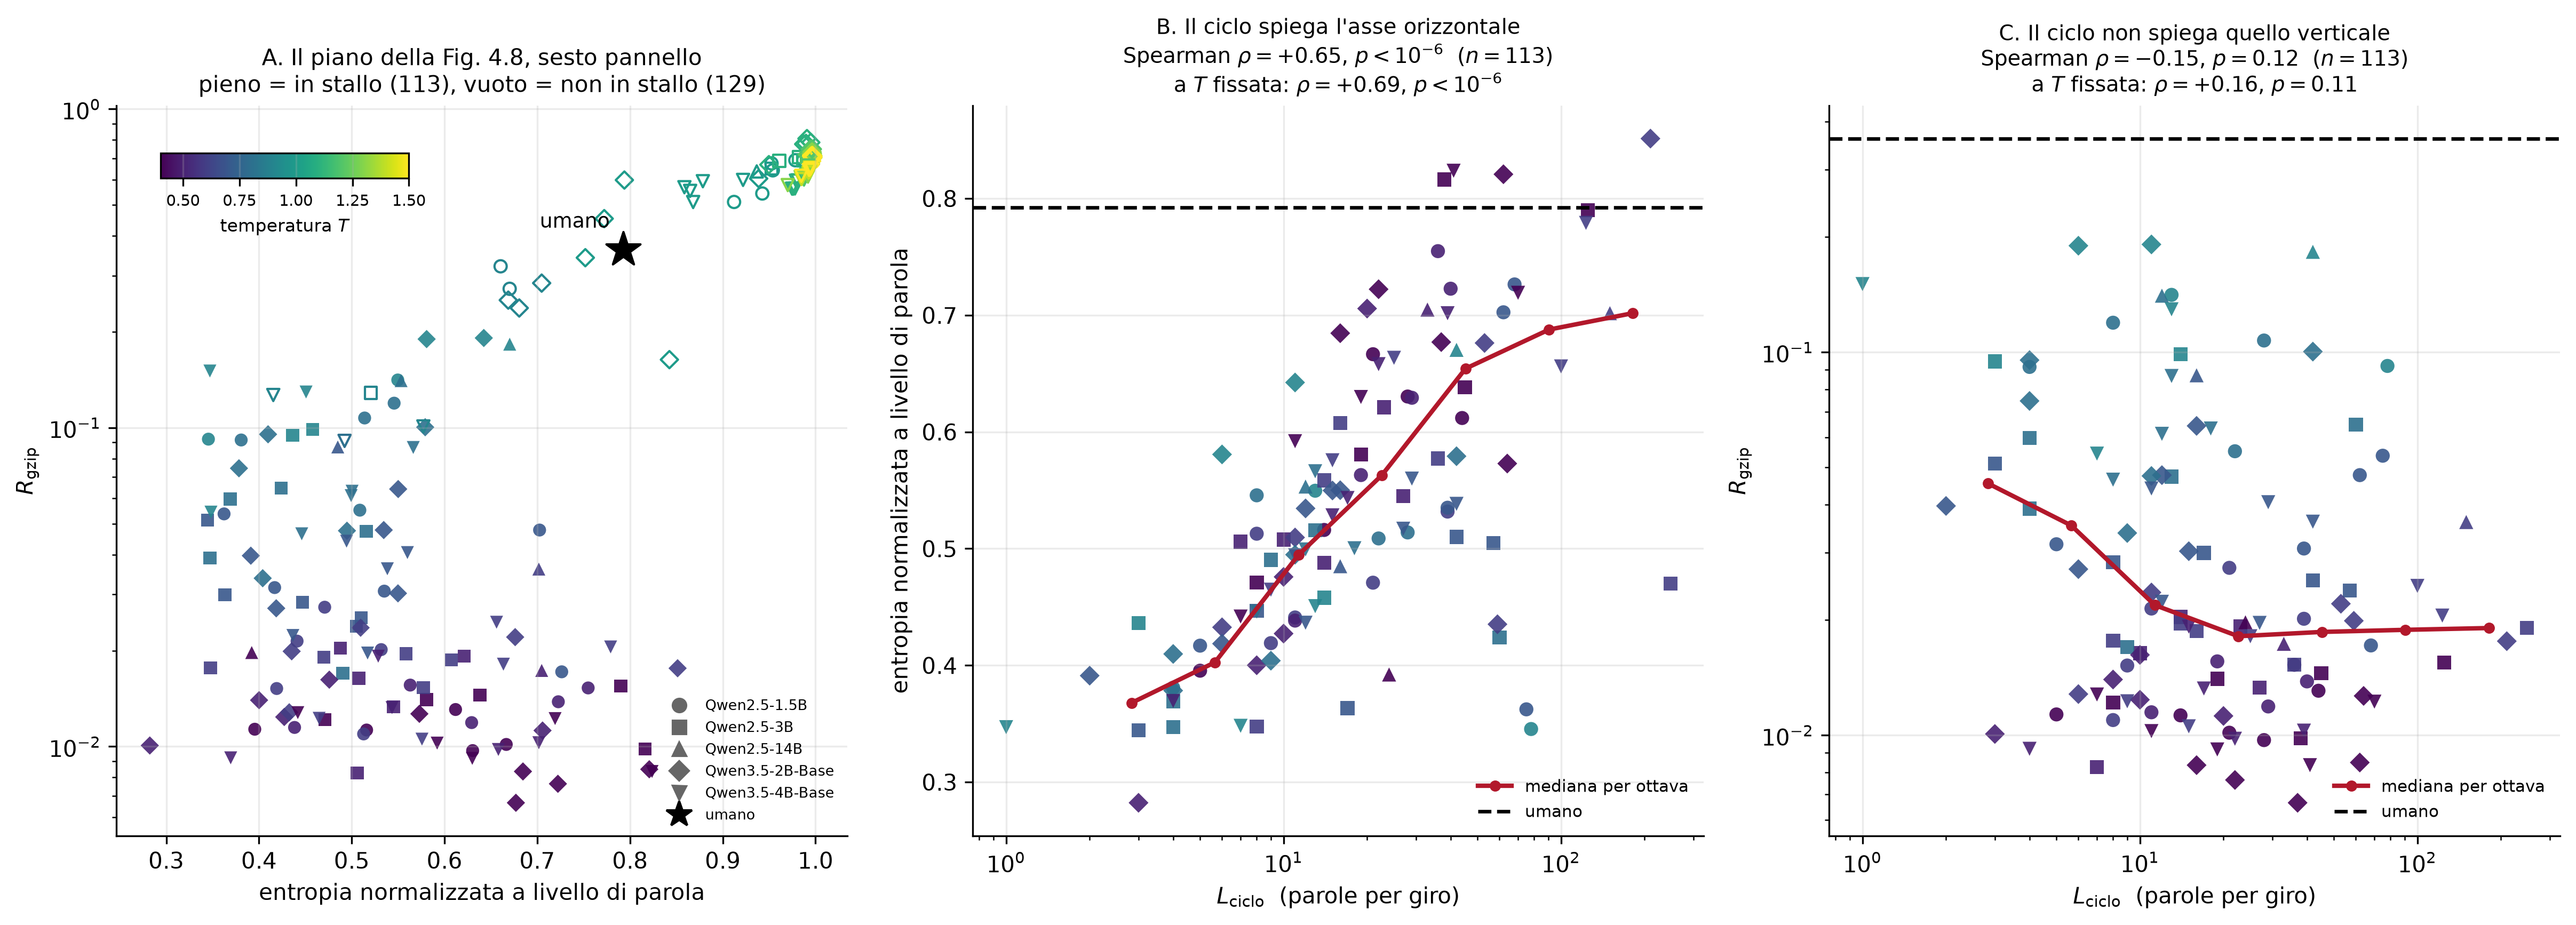
\includegraphics[width=\textwidth]{figure/cap4_ciclo_entropia.png}
  \caption{Lunghezza del ciclo ripetuto in fase di stallo. A: il piano
  entropia--comprimibilità della Figura~\ref{fig:compressione}, con i documenti
  in stallo a simbolo pieno e gli altri a simbolo vuoto; il colore codifica la
  temperatura e la forma il modello. B: entropia di parola contro lunghezza del
  ciclo, con la mediana per ottava. C: rapporto di compressione contro la stessa
  grandezza. La lunghezza del ciclo ordina l'asse orizzontale del piano e non
  quello verticale.}
  \label{fig:ciclo}
\end{figure}


% ---------------------------------------------------------------------
\section{Le tre fasi}
\label{sec:fasi-risultati}

Le misure precedenti descrivono il testo generato senza classificarlo. La regola
del §\ref{sec:tre-fasi} permette invece di assegnare ciascun documento a una
fase, e questa sezione ne riporta l'esito.

La traiettoria della~\eqref{eq:traiettoria} è costruita sui vettori GloVe a 100
dimensioni già impiegati nel §\ref{sec:token}, e l'autocorrelazione è calcolata
sui primi cento lag, misurati in parole. Il fit del GAPELMAPER usa invece un
intervallo più ampio, fino a 600 parole, perché distinguere una legge di potenza
da un esponenziale richiede più di una decade di distanze. Il livello di rumore
$\eta$ è stimato su una singola permutazione della traiettoria di ciascun
documento, con seme fissato.

Le due soglie della regola valgono $\kappa_{\min} = 0.50$ e $\Phi_{\min} = 3$.
La prima è deliberatamente permissiva: serve a escludere i documenti in cui meno
di metà delle parole ha un vettore, cioè quelli in cui la traiettoria è fatta per
lo più di zeri, e non a selezionare i documenti buoni. La seconda separa i due
gruppi in cui $\Phi$ effettivamente si distribuisce, e la sua posizione è poco
critica: come mostra la Figura~\ref{fig:transizioni}, fra la fase periodica e
quella successiva $\Phi$ cambia di due ordini di grandezza, cosicché qualunque
soglia compresa fra $1$ e $5$ produce la stessa classificazione. Il
§\ref{sec:tstar} riprende il punto trattando la fine della fase periodica come
uno degli otto criteri di temperatura critica.

La Figura~\ref{fig:acf} mostra come questa autocorrelazione cambia lungo lo
sweep. Fino a $T = 0.9$ la curva oscilla con periodo definito e ampiezza
prossima all'unità: il testo ripete un ciclo di parole, e a distanza pari a un
multiplo del ciclo ogni vettore ritrova sé stesso. Il periodo si accorcia al
crescere della temperatura, da dieci parole a $T = 0.5$ a circa tre a $T =
0.8$, mentre l'ampiezza scende da $0.98$ a $0.72$. Fra $T = 0.9$ e $T = 1.0$
la struttura periodica scompare del tutto: l'ampiezza cade a $0.036$ e la
curva diventa un decadimento monotono, senza più oscillazione. A $T = 1.3$
l'intera curva è contenuta nella banda di rumore stimata mescolando le parole
del documento, cioè non è distinguibile dal caso.

Il confronto con il testo umano chiarisce quanto entrambi i regimi siano
lontani dal linguaggio naturale. L'autocorrelazione del romanzo non è
periodica, con $\max\lvert\mathrm{FFT}\rvert$ pari a $1.16$, ben sotto la
soglia $3$, ma è nettamente sopra il livello di rumore su tutti i cento lag
esaminati, e il suo spettro decade in modo regolare invece di essere piatto.
Nessuna delle temperature campionate riproduce questa combinazione: sotto la
transizione la correlazione è troppo forte e periodica, sopra è assente.

\begin{figure}[htbp]
  \centering
  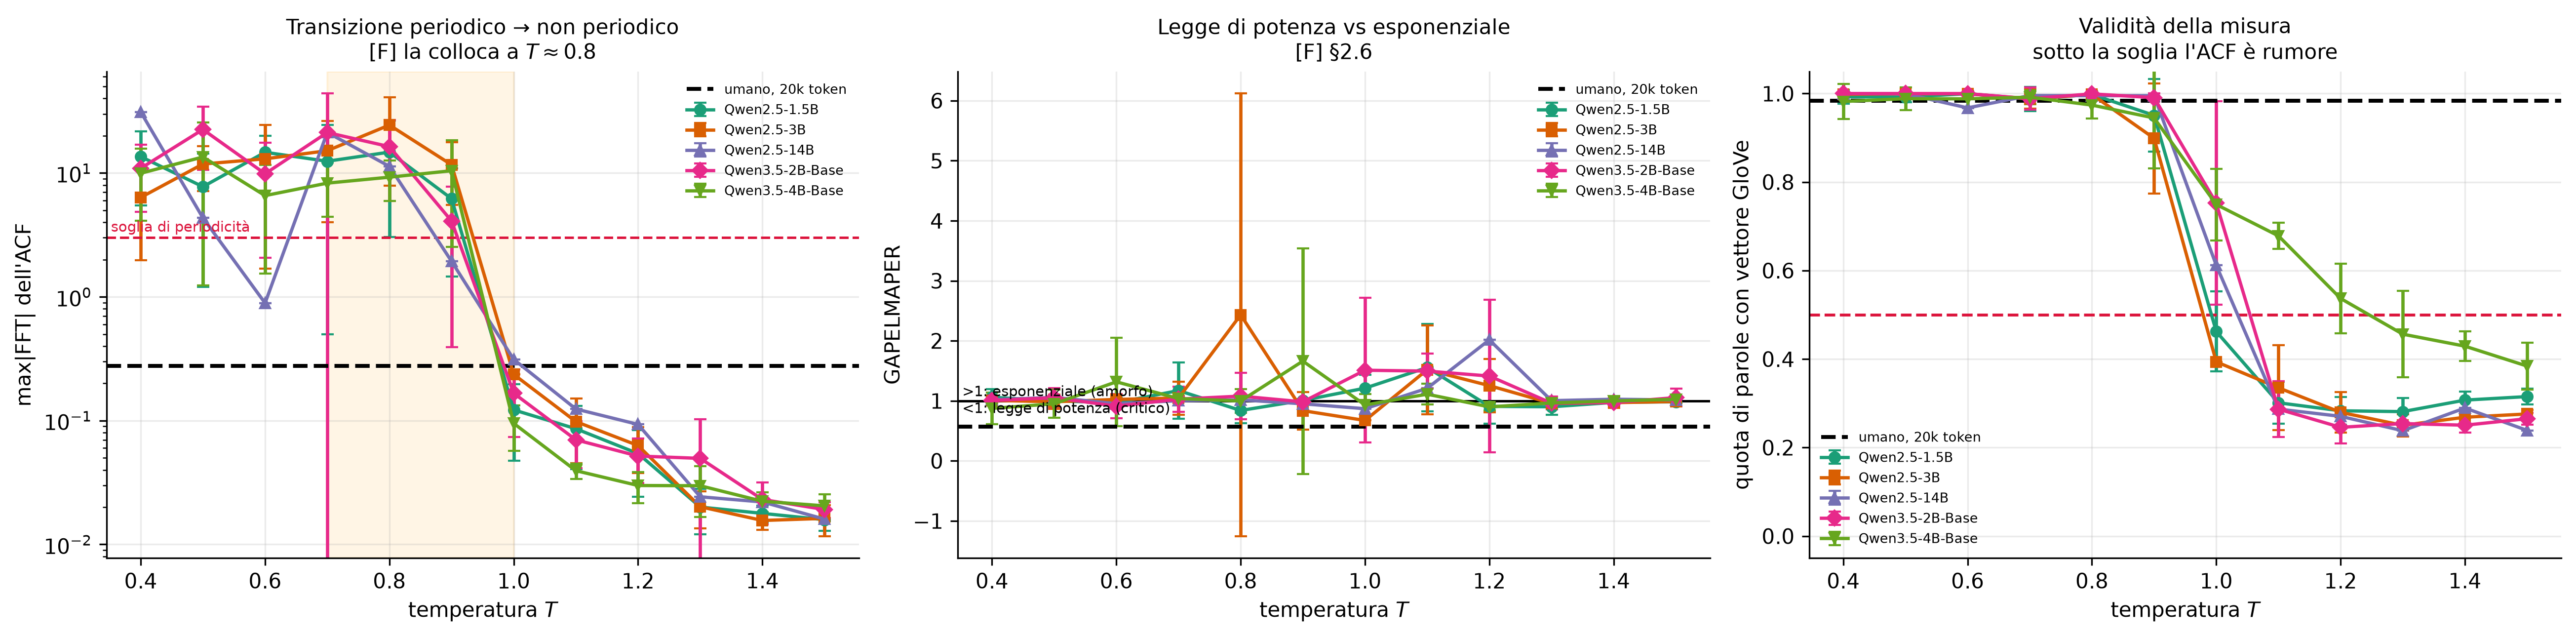
\includegraphics[width=\textwidth]{figure/cap4_transizioni_fase.png}
  \caption{Parametro di periodicità, GAPELMAPER e copertura degli embedding in
  funzione della temperatura. Il primo pannello è in scala logaritmica. Il terzo
  riporta la quota di parole dotate di un vettore, che è la condizione di
  validità delle altre due misure.}
  \label{fig:transizioni}
\end{figure}

\begin{figure}[htbp]
  \centering
  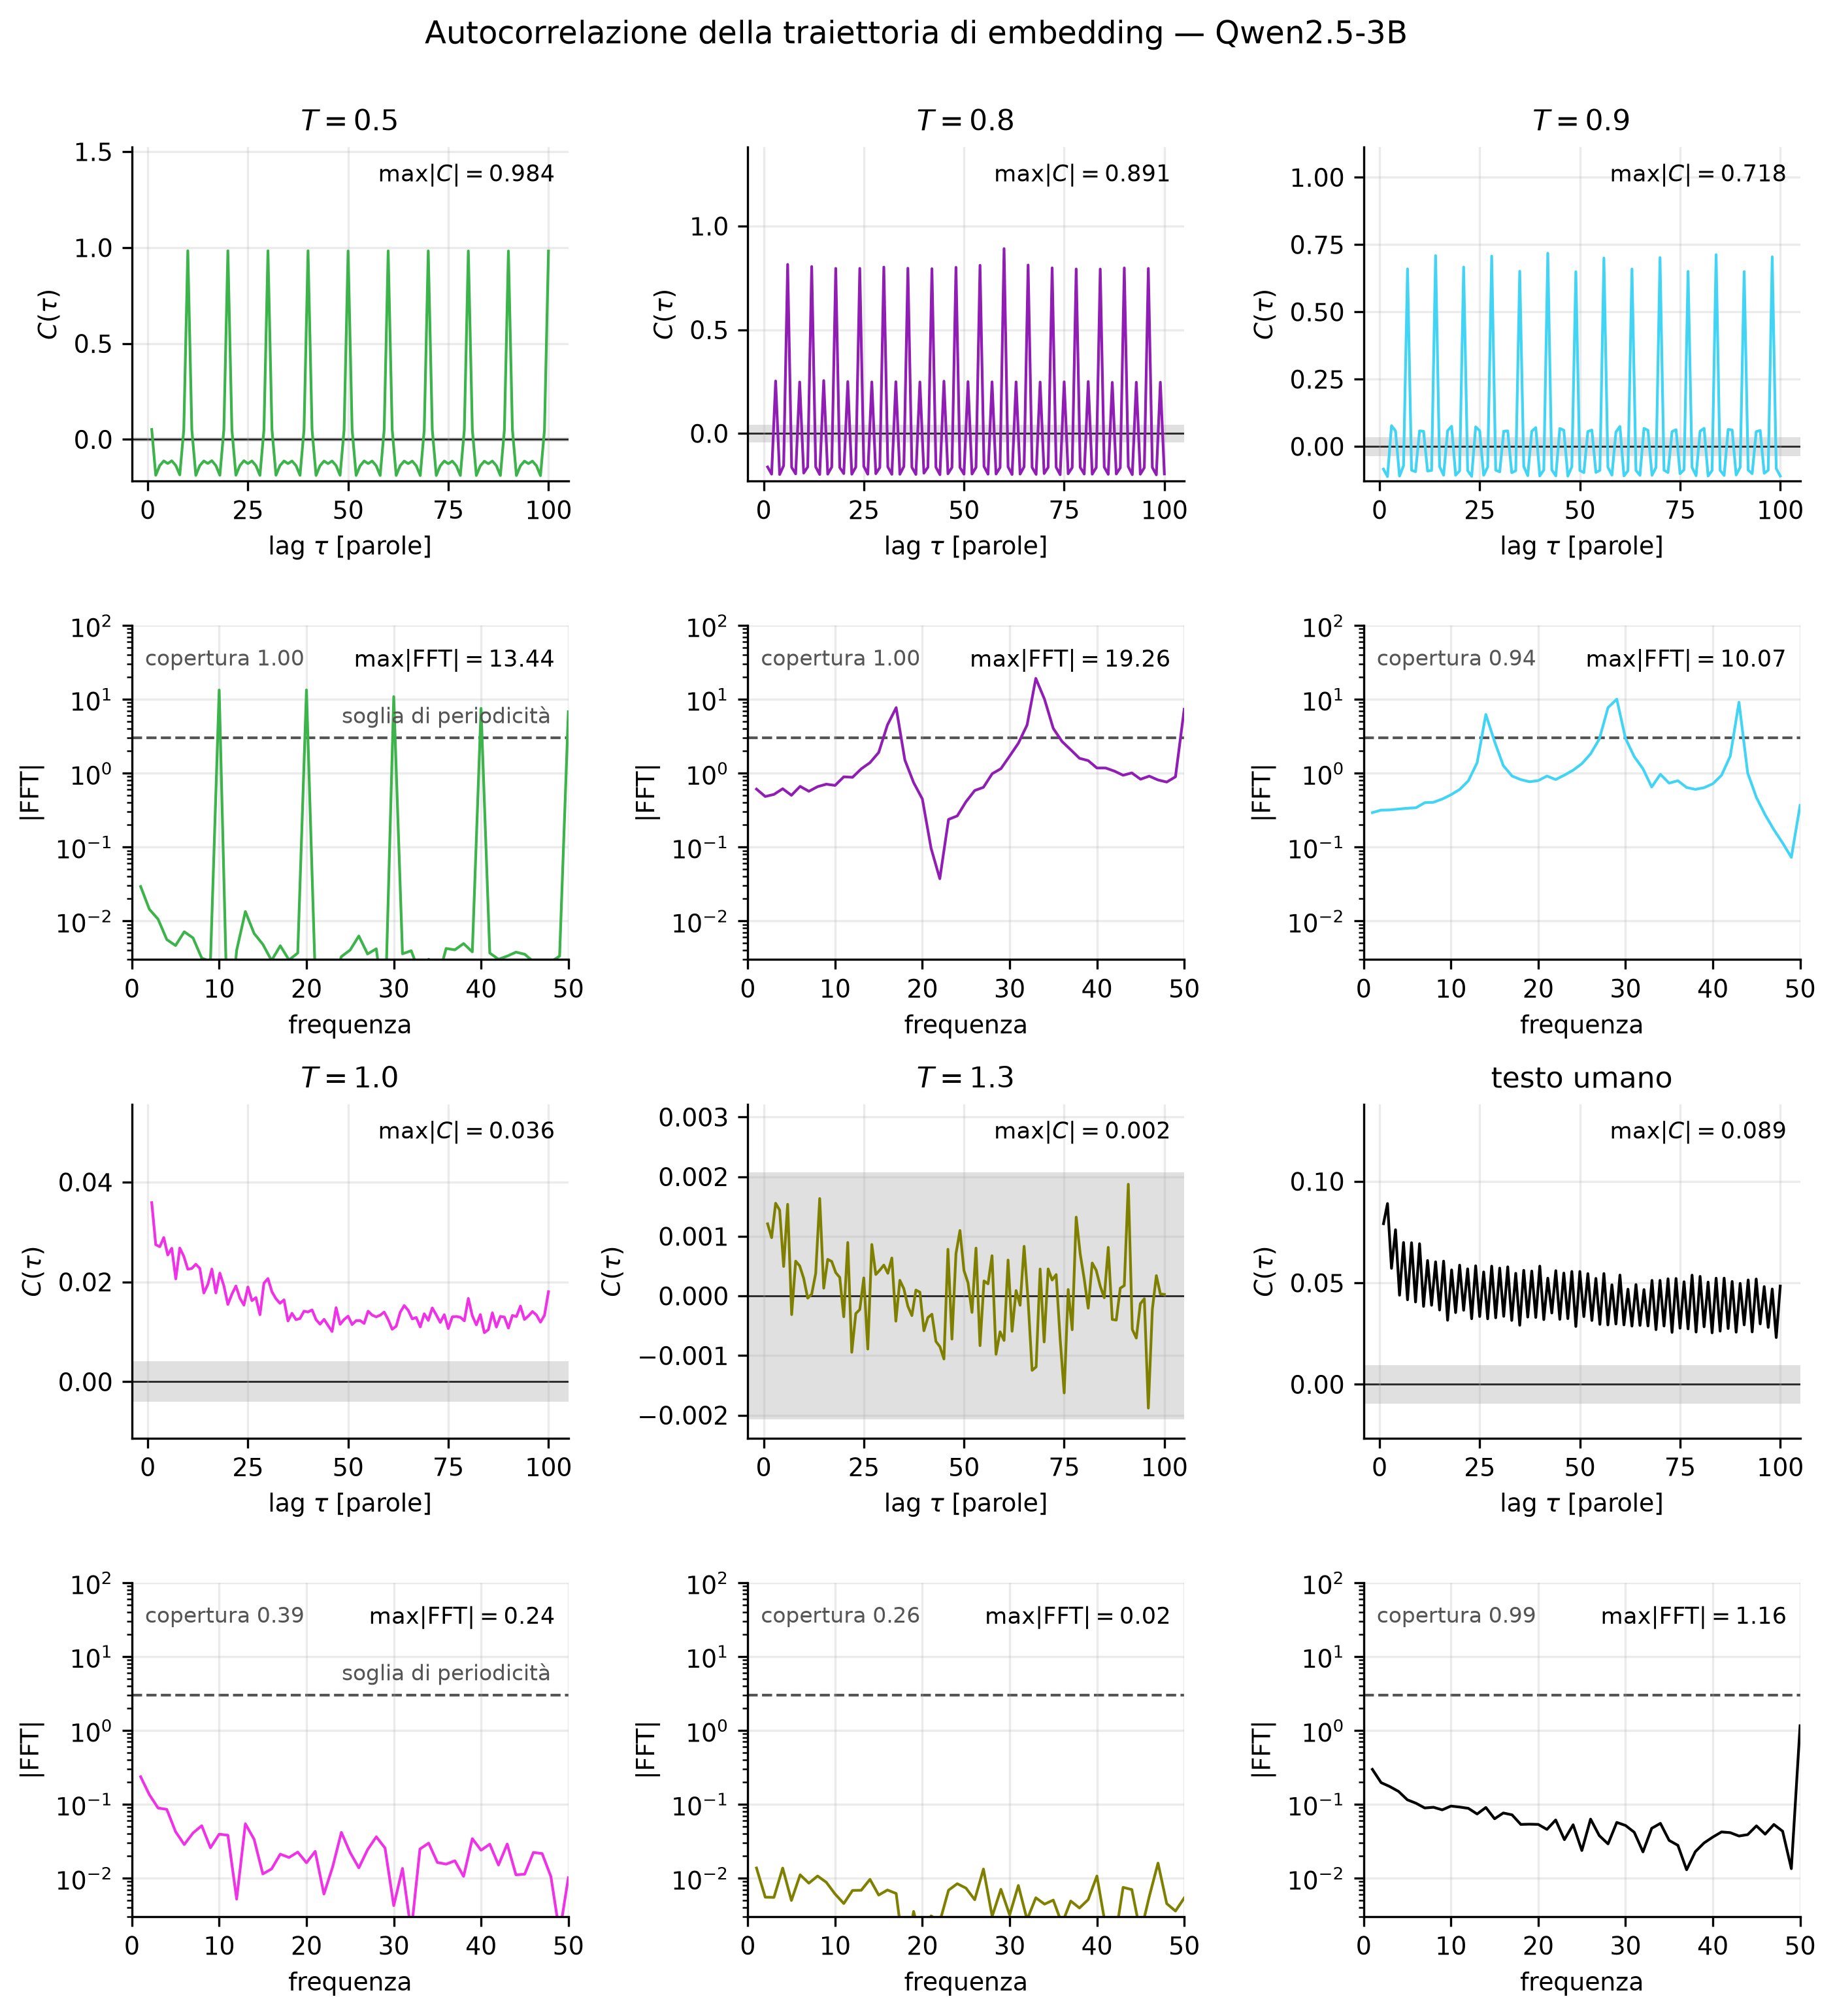
\includegraphics[width=\textwidth]{figure/cap4_acf_Qwen25_3B.png}
  \caption{Autocorrelazione della traiettoria di embedding per il modello
  Qwen2.5-3B a cinque temperature e sul testo umano di riferimento. In ciascuna
  coppia di riquadri il primo riporta $C(\tau)$ per lag da 1 a 100 parole e il
  secondo il modulo della sua trasformata di Fourier. La banda grigia è il
  livello di rumore, stimato ricalcolando $C(\tau)$ dopo aver permutato a caso
  le parole dello stesso documento; la linea tratteggiata è la soglia
  $\max\lvert\mathrm{FFT}\rvert = 3$ che separa la fase periodica. Per ogni
  temperatura è mostrato il campione di periodicità mediana, non il più marcato.
  La scala verticale di $C(\tau)$ è propria di ciascun riquadro, perché
  l'ampiezza varia di oltre due ordini di grandezza fra le temperature basse e
  quelle alte; il valore di picco è riportato dentro il riquadro. La scala dello
  spettro è invece logaritmica e comune, così i sei casi si confrontano
  direttamente.}
  \label{fig:acf}
\end{figure}

Il parametro d'ordine della prima transizione è il massimo modulo della
trasformata oltre il primo coefficiente, e il suo crollo è il risultato più
netto dell'intero capitolo. La media su tutti i modelli vale $16.0$ a
$T = 0.8$, scende a $7.5$ a $T = 0.9$ e precipita a $0.145$ a $T = 1.0$: un
fattore cinquanta in un solo passo di temperatura, e cento rispetto al massimo
di $T = 0.8$. Prosegue poi fino a $0.018$ a
$T = 1.5$, complessivamente tre ordini di grandezza sotto il massimo. Le cinque
curve dei diversi modelli si sovrappongono quasi esattamente, come mostra la
Figura~\ref{fig:transizioni}.

Anche questa soglia va confrontata con la fonte.
In~\cite{mikhaylovskiy2025states} la transizione dalla fase periodica è
collocata attorno a $t = 0.8$, con il testo dichiarato già non periodico a
$t = 1$, mentre qui la periodicità sopravvive fino a $T = 0.9$ e scompare a
$T = 1.0$. Lo spostamento verso l'alto è coerente con l'effetto del prompt
descritto nel §\ref{sec:protocollo}, che ritarda la comparsa delle proprietà
del regime disordinato.

\paragraph{Il secondo criterio non discrimina.} La distinzione fra stato
critico e fase amorfa dovrebbe essere operata dal GAPELMAPER, ma sui dati di
questo lavoro tale criterio non funziona. Il suo valore medio è $1.101$ con
deviazione standard $0.677$, e la quota di documenti con valore inferiore a 1,
cioè classificati come critici, è $0.51$: una moneta. Le barre d'errore nel
pannello centrale della Figura~\ref{fig:transizioni} sono di ampiezza
confrontabile con l'intero intervallo di variazione.

La difficoltà non è propria di questi dati. Lo stesso
\cite{mikhaylovskiy2025states} riporta che sui testi Qwen il GAPELMAPER è
raramente inferiore a 1, e che a diverse temperature del suo sweep non è
calcolabile affatto perché l'autocorrelazione assume valori negativi. Il
criterio, insomma, discrimina male anche nel lavoro che lo introduce.

Il motivo emerge dal terzo pannello. La copertura degli embedding resta sopra il
$95\%$ fino a $T = 0.9$, ma crolla a $0.64$ a $T = 1.0$ e a circa $0.31$ oltre
$T = 1.2$: nel regime in cui il GAPELMAPER dovrebbe distinguere le ultime due
fasi, l'autocorrelazione è calcolata su una minoranza delle parole e non
contiene più segnale. Per questa ragione i documenti che non superano la soglia
di copertura sono marcati come non valutabili anziché classificati, come
anticipato nel §\ref{sec:tre-fasi}. Senza tale precauzione il criterio avrebbe
assegnato una fase a documenti in cui non c'è nulla da misurare.

\paragraph{Il diagramma di fase.}
La Figura~\ref{fig:diagramma} riporta la composizione delle fasi per modello e
temperatura. Il quadro è coerente su tutti e cinque: fase periodica fino a
$T = 0.9$, dove la classificazione è ancora periodica per 13 documenti su 18;
scomparsa completa della periodicità a $T = 1.0$; documenti prevalentemente non
valutabili da $T = 1.1$ in poi, e completamente tali a $T \ge 1.4$.

\begin{figure}[htbp]
  \centering
  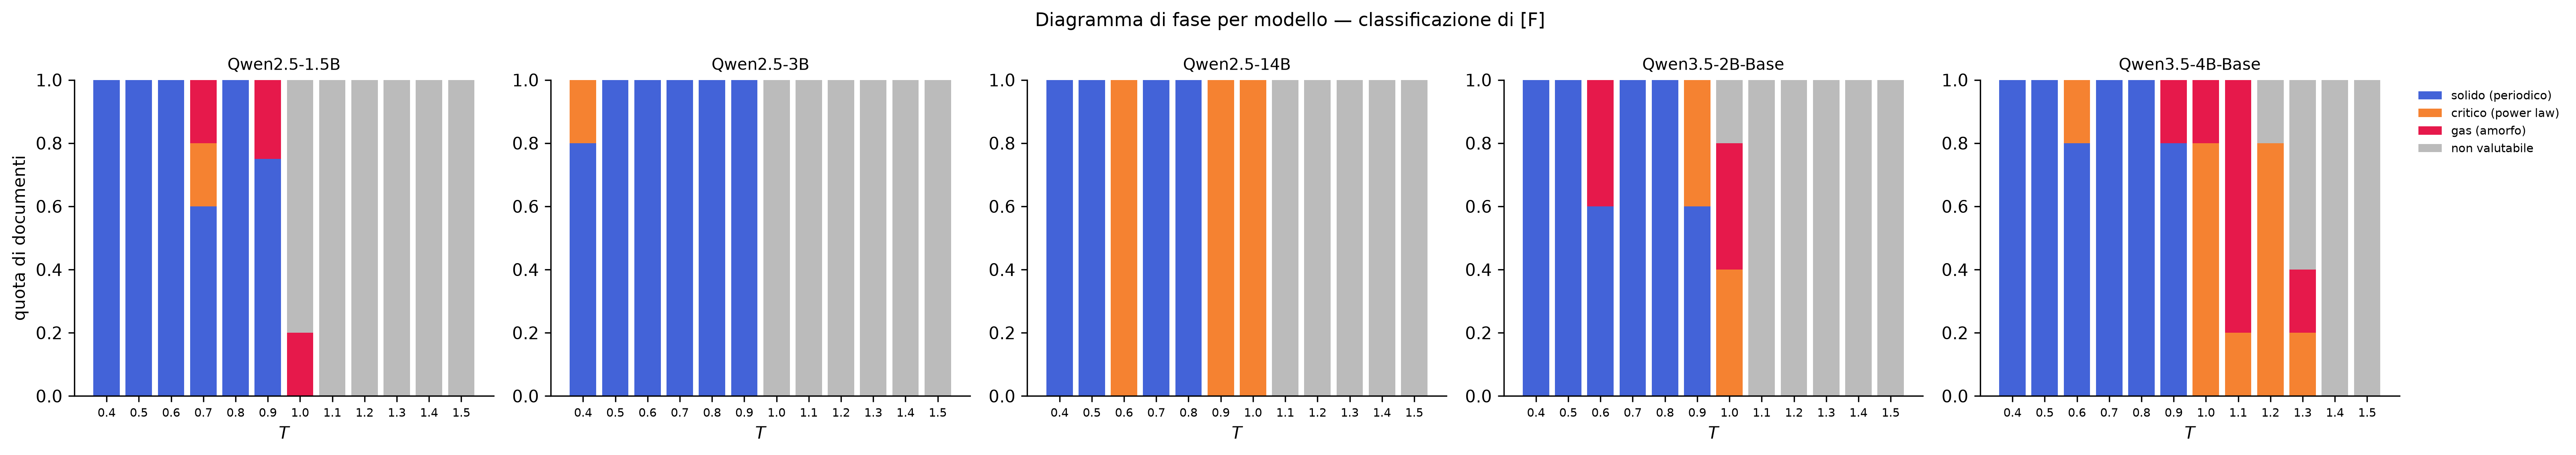
\includegraphics[width=\textwidth]{figure/cap4_diagramma_fase.png}
  \caption{Composizione delle fasi per modello e temperatura. La categoria «non
  valutabile» raccoglie i documenti che non superano la soglia di copertura
  degli embedding.}
  \label{fig:diagramma}
\end{figure}

Le tre modalità di fallimento del §\ref{sec:fallimenti} trovano qui la loro
interpretazione. La degenerazione per ripetizione è la fase periodica; la
degenerazione dell'alfabeto e del lessico corrisponde alla regione in cui la
misura non è più applicabile, che è a sua volta il segnale della fase amorfa. Il
testo non degenerato esiste solo nella striscia sottile fra le due, ed è la
stessa striscia in cui tutte le misure delle sezioni precedenti si avvicinano ai
valori umani.

% ---------------------------------------------------------------------
\section{Convergenza della temperatura critica}
\label{sec:tstar}

Le sezioni precedenti individuano ciascuna una temperatura privilegiata. Poiché
i criteri provengono da lavori indipendenti e misurano proprietà diverse del
testo, il loro accordo o disaccordo è esso stesso un risultato.

La Tabella~\ref{tab:tstar} riporta la temperatura selezionata da ciascun
criterio per ciascun modello. Due criteri sono intrinseci, nel senso che
individuano un estremo della curva senza far riferimento al testo umano: il
minimo del MAPE e la fine della fase periodica. Gli altri sei selezionano la
temperatura alla quale la misura si avvicina di più alla baseline umana.

\begin{table}[htbp]
\centering
\small
\begin{tabular}{@{}lccccc@{}}
\toprule
Criterio & 1.5B & 3B & 14B & 3.5-2B & 3.5-4B \\
\midrule
MAPE minimo                                  & 0.9 & 0.9 & 0.7 & 0.9 & 0.9 \\
$D_s$ minima dal testo umano                 & 0.9 & 0.9 & 0.9 & 0.9 & 1.0 \\
Fine della fase periodica                    & 1.0 & 1.0 & 0.6 & 1.0 & 1.0 \\
$R_{\mathrm{gzip}}$ più vicino all'umano     & 0.9 & 1.0 & 0.9 & 1.0 & 1.0 \\
$\alpha$ più vicino all'umano                & 1.0 & 1.5 & 1.3 & 1.0 & 1.0 \\
$R$ più vicino all'umano                     & 1.0 & 1.1 & 1.1 & 1.1 & 1.0 \\
$\gamma_H$ più vicino all'umano              & 1.1 & 1.0 & 1.3 & 1.1 & 1.3 \\
$\alpha_{\mathrm{DFA}}$ più vicino all'umano & 1.2 & 1.1 & 1.1 & 1.1 & 1.1 \\
\midrule
\textbf{mediana}                             & \textbf{1.0} & \textbf{1.0} &
\textbf{1.0} & \textbf{1.0} & \textbf{1.0} \\
\bottomrule
\end{tabular}
\caption{Temperatura selezionata da ciascun criterio, per ciascun modello. La
mediana vale $1.0$ per tutti e cinque i modelli, benché i singoli criteri
spazino da $0.6$ a $1.5$.}
\label{tab:tstar}
\end{table}

Il risultato principale del capitolo è la riga in fondo alla tabella. Otto
criteri tratti da quattro lavori indipendenti, costruiti per scopi diversi e mai
progettati per concordare, danno una mediana identica per tutti e cinque i
modelli. La convergenza non era scontata: i criteri misurano la distribuzione
delle frequenze, la crescita del vocabolario, le correlazioni a lungo raggio, la
comprimibilità e la periodicità dell'autocorrelazione, cioè proprietà che nulla
obbliga a coincidere.

\begin{figure}[htbp]
  \centering
  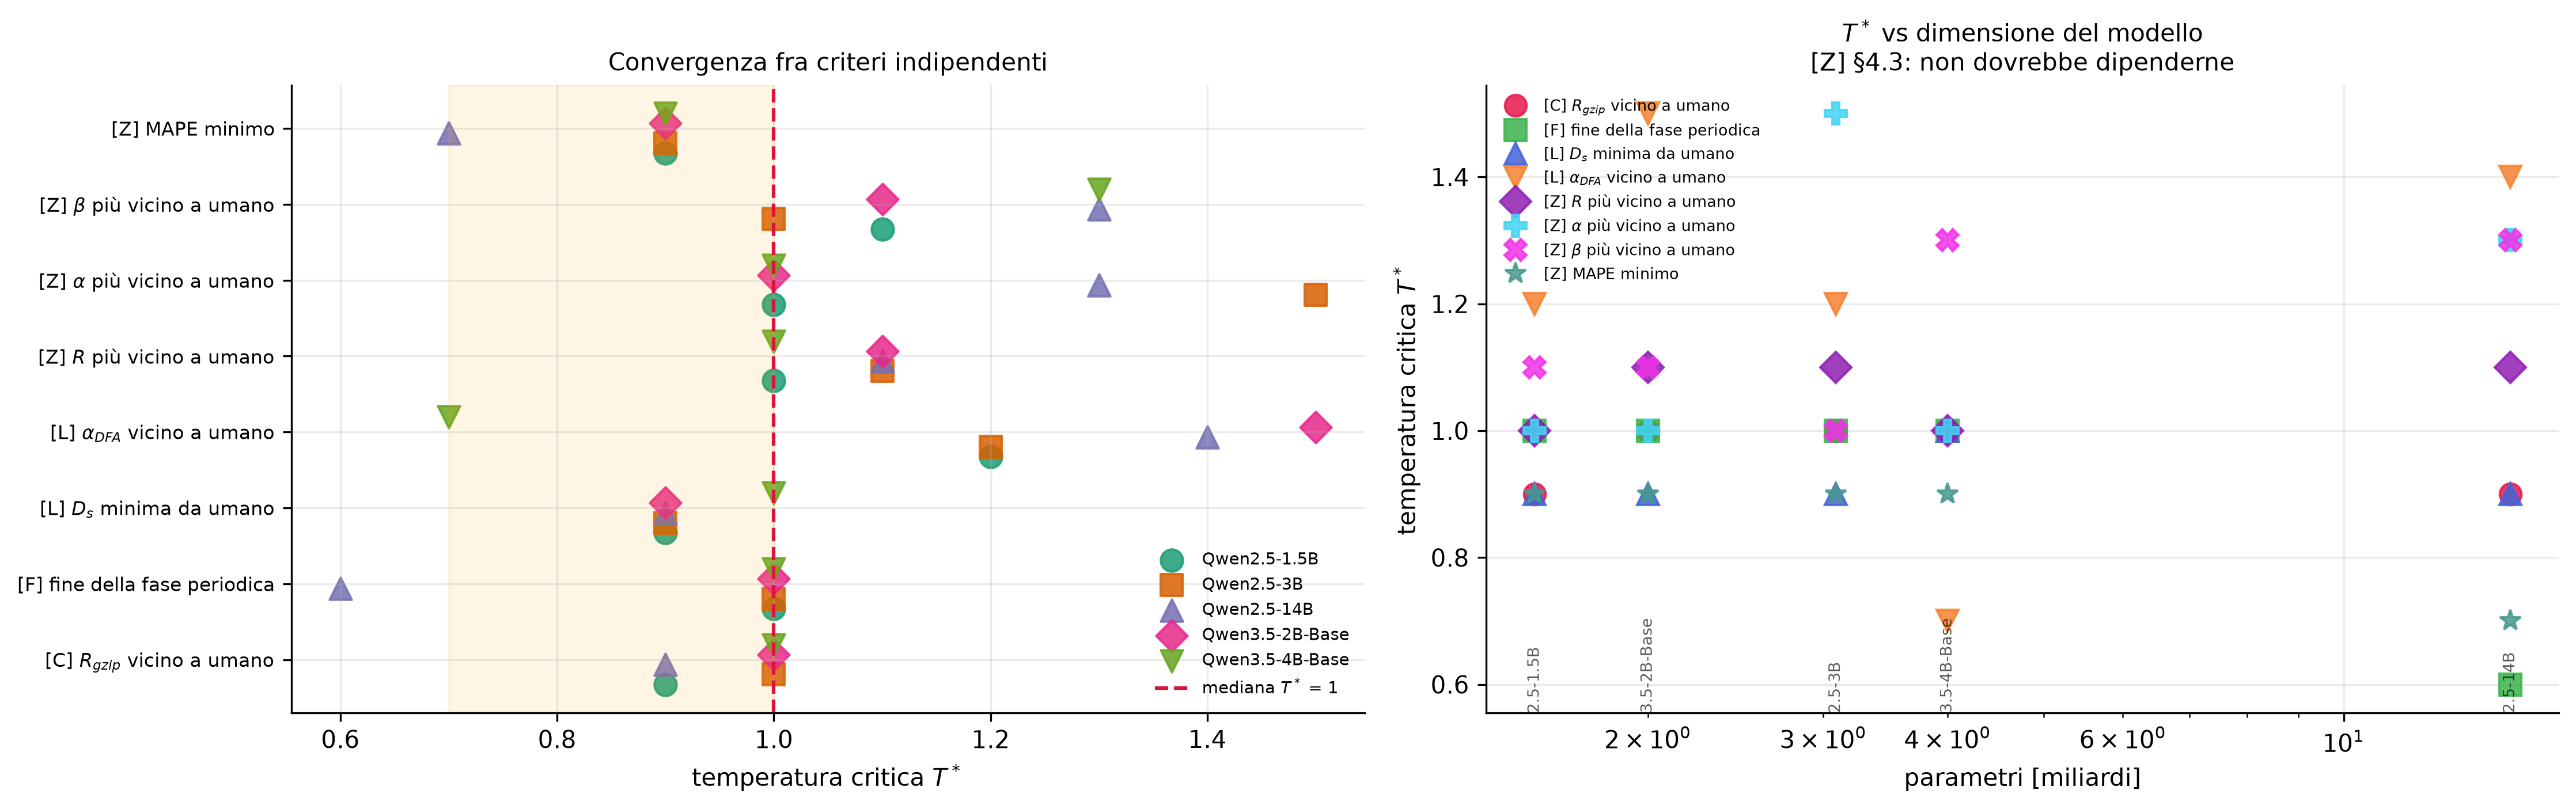
\includegraphics[width=\textwidth]{figure/cap4_temperatura_critica.png}
  \caption{A sinistra, la temperatura selezionata da ciascun criterio; la linea
  tratteggiata è la mediana complessiva e la banda la regione fra $0.7$ e $1.0$.
  A destra, la stessa quantità in funzione del numero di parametri del modello.}
  \label{fig:tstar}
\end{figure}

\paragraph{Dipendenza dalla dimensione del modello.}
La Figura~\ref{fig:tstar} riporta a destra la temperatura critica in funzione
del numero di parametri. La correlazione di rango è $\rho = -0.01$ con
$p = 0.93$ su quaranta osservazioni: nessuna dipendenza rilevabile. Il dato è
coerente con quanto riportato in~\cite{mikhaylovskiy2025zipf}, dove la posizione
dell'ottimo risulta indipendente dalla dimensione per tutte le famiglie
esaminate.

Un'assenza di correlazione misurata su cinque modelli appartenenti a due
famiglie non dimostra l'indipendenza: dimostra che, entro l'intervallo di
dimensioni esplorato e con la potenza statistica disponibile, non emerge
alcuna dipendenza. È coerenza con la letteratura, non conferma indipendente.

\paragraph{Una discordanza fra criteri.}
Due criteri si collocano sistematicamente fuori dal gruppo, e la loro distanza
dagli altri è essa stessa un risultato: mediarli insieme al resto la
cancellerebbe.

Il minimo del MAPE cade a $0.9$, mentre la fine della fase periodica cade a
$1.0$: alla temperatura in cui la distribuzione delle frequenze è più vicina a
una legge di potenza, l'autocorrelazione è ancora periodica per la maggioranza
dei documenti. Le due misure non si contraddicono, perché guardano oggetti
diversi, la statistica dei conteggi l'una e la struttura sequenziale l'altra,
e la loro distanza quantifica il fatto che le due proprietà non compaiono
simultaneamente. Il testo acquista una distribuzione di frequenze verosimile
prima di perdere la ripetizione.

Il criterio basato su $\alpha_{\mathrm{DFA}}$ merita una nota, perché il suo
esito dipende dall'ordine del detrending. Con il grado 1 seleziona temperature
fra $0.7$ e $1.5$, il più disperso dei nove; con il grado 2, che è quello
adottato qui per la ragione data nel §\ref{sec:robustezza}, si allinea agli
altri e sceglie $1.1$ per quattro modelli su cinque. La mediana per modello vale
$1.0$ in entrambi i casi. Resta valida l'avvertenza del
§\ref{sec:dfa-risultati}: alle basse temperature quell'esponente è instabile
fra documenti, e viene riportato per completezza anziché usato come criterio a
sé stante.

Una divergenza analoga fra criteri è documentata
in~\cite{mikhaylovskiy2025zipf} per i modelli Llama di grandi dimensioni, dove
le leggi di Zipf e di Heaps individuano temperature critiche sensibilmente
diverse. Il fenomeno non sembra dunque un artefatto di questo lavoro.

% ---------------------------------------------------------------------
\section{Che cosa lo sweep ha stabilito}
\label{sec:sintesi-cap4}

Tre risultati emergono dalle sezioni precedenti, di natura diversa fra loro.

Il primo è l'esistenza di una temperatura privilegiata, e la sua posizione. Otto
criteri costruiti per scopi diversi e tratti da quattro lavori indipendenti
danno una mediana identica, $T = 1.0$, per tutti e cinque i modelli, senza
dipendenza rilevabile dalla dimensione. Il secondo è che l'ottimo è stretto: la
transizione si consuma quasi interamente fra $T = 0.9$ e $T = 1.0$, dove il
parametro di periodicità cade di un fattore cinquanta, l'entropia passa da
$0.332$ a $5.77$ bit per carattere e il rapporto di compressione da $0.107$ a
$0.650$. Uno sweep a passo $0.1$ è appena sufficiente a risolvere quella
finestra.

Il terzo è l'esito negativo su cui poggia il capitolo successivo. L'esistenza
dell'ottimo è un fatto generale, ma la sua \emph{qualità} non lo è: due modelli
su cinque portano il MAPE al livello del testo umano e gli altri no. La
compressione condizionata non raggiunge il valore umano a nessuna temperatura,
ma per una ragione che non riguarda la struttura semantica: sotto la transizione
il testo ripete un ciclo e la seconda metà è prevedibile per costruzione, sopra
non è più linguaggio e non è prevedibile da nulla. Soprattutto, i documenti che
superano tutte e tre le soglie di non
degenerazione sono due su \num{242}. Il corpus generato lungo lo sweep non
sostiene quindi un'analisi semantica, ed è la ragione per cui il
Capitolo~\ref{cap:risultati2} cambia dominio anziché proseguire su questo.

Il capitolo non stabilisce però tutto. La convergenza dei criteri dice dove il
testo generato somiglia di più a quello umano secondo misure che ignorano il
significato; non dice se in quel punto il testo sia organizzato attorno a un
contenuto. È la domanda posta nel §\ref{sec:intro-domanda}, e richiede gli
strumenti del §\ref{sec:burst}.
%  Figure del corpo: modello Qwen2.5-3B. Quelle degli altri quattro
%  modelli stanno nel repository indicato in Appendice A.
% =====================================================================

\chapter{Il testo generato lungo lo sweep di temperatura}
\label{cap:risultati1}

Questo capitolo applica ai \num{242} documenti generati le misure introdotte nel
Capitolo~\ref{cap:teoria}, facendo variare la sola temperatura di campionamento.
Ogni misura viene confrontata con la baseline umana della
Tabella~\ref{tab:baseline}, calcolata con le stesse procedure e alla stessa
lunghezza.

Le figure del corpo del capitolo mostrano il modello Qwen2.5-3B, scelto come
esemplare perché dispone di cinque campioni per quasi tutte le temperature e
presenta le curve meno rumorose; le corrispondenti figure per gli altri quattro
modelli sono depositate nel repository indicato
nell'Appendice~\ref{app:codice}. Le curve aggregate
riportano invece tutti e cinque i modelli.

Il risultato principale non è nessuna delle singole misure, ma il fatto che
convergano: criteri tratti da quattro lavori indipendenti, costruiti per scopi
diversi, individuano la stessa regione di temperature. Il §\ref{sec:tstar} lo
documenta.

% ---------------------------------------------------------------------
\section{Le tre modalità di fallimento}
\label{sec:fallimenti}

La prima e la terza riga della Tabella~\ref{tab:tre-regimi} sono entrambe
prodotte dai modelli qui analizzati, a due temperature diverse, e mostrano i
due modi in cui la generazione si allontana dal linguaggio: la ripetizione letterale a bassa
temperatura, l'incoerenza semantica ad alta temperatura. Salendo ancora si
incontra un terzo regime, in cui l'alfabeto stesso si disgrega e il testo diventa
un miscuglio di sistemi di scrittura diversi.

Le tre modalità possono essere separate quantitativamente. Un documento viene
classificato come degenerato per \emph{ripetizione} se la quota di 8-grammi
ripetuti supera $0.10$, contro il valore $0.000$ misurato sul testo umano; come
degenerato nell'\emph{alfabeto} se la quota di caratteri non ASCII supera
$0.05$, più del triplo del valore umano $0.014$; come degenerato nel
\emph{lessico} se meno del $70\%$ delle sue parole possiede un vettore nello
spazio di embedding, contro il $98\%$ del testo umano. Le tre condizioni non si
escludono a vicenda, e un documento può soddisfarne più di una.

La Tabella~\ref{tab:fallimenti} riporta i conteggi.

\begin{table}[htbp]
\centering
\small
\begin{tabular}{@{}l>{\raggedright\arraybackslash}p{5.4cm}rr@{}}
\toprule
Modalità & Criterio & Documenti & Quota \\
\midrule
Ripetizione & 8-grammi ripetuti $> 0.10$      & 122 & 50\,\% \\
Alfabeto    & caratteri non ASCII $> 0.05$    & 125 & 52\,\% \\
Lessico     & copertura degli embedding $< 0.70$ & 112 & 46\,\% \\
\midrule
Nessuna     & prosa inglese non degenerata    &   2 &  1\,\% \\
\bottomrule
\end{tabular}
\caption{Modalità di degenerazione dei \num{242} documenti generati. Le
categorie non sono disgiunte. La classificazione dipende dalle soglie scelte,
ma non nella sostanza: facendole variare entro intervalli ragionevoli il numero
di documenti non degenerati resta compreso fra 2 e 7, cioè fra l'uno e il tre
per cento del totale.}
\label{tab:fallimenti}
\end{table}

Il dato va letto con attenzione, perché è il presupposto dell'intera seconda
parte sperimentale. Non significa che i modelli siano incapaci di produrre
linguaggio, ma che la finestra di temperature in cui lo producono è
sufficientemente stretta da non essere coperta da uno sweep a passo $0.1$: i
soli due documenti non degenerati compaiono a $T = 1.0$, e già a $T = 0.9$ e
$T = 1.1$ tutti i campioni ricadono in almeno una delle tre categorie. Il
Capitolo~\ref{cap:risultati2} muove da questa constatazione.


% ---------------------------------------------------------------------
\section{Legge di Zipf}
\label{sec:zipf-risultati}

La Figura~\ref{fig:zipf-cum} riporta gli istogrammi cumulativi delle frequenze,
una curva per temperatura, con la curva umana per confronto.

\begin{figure}[htbp]
  \centering
  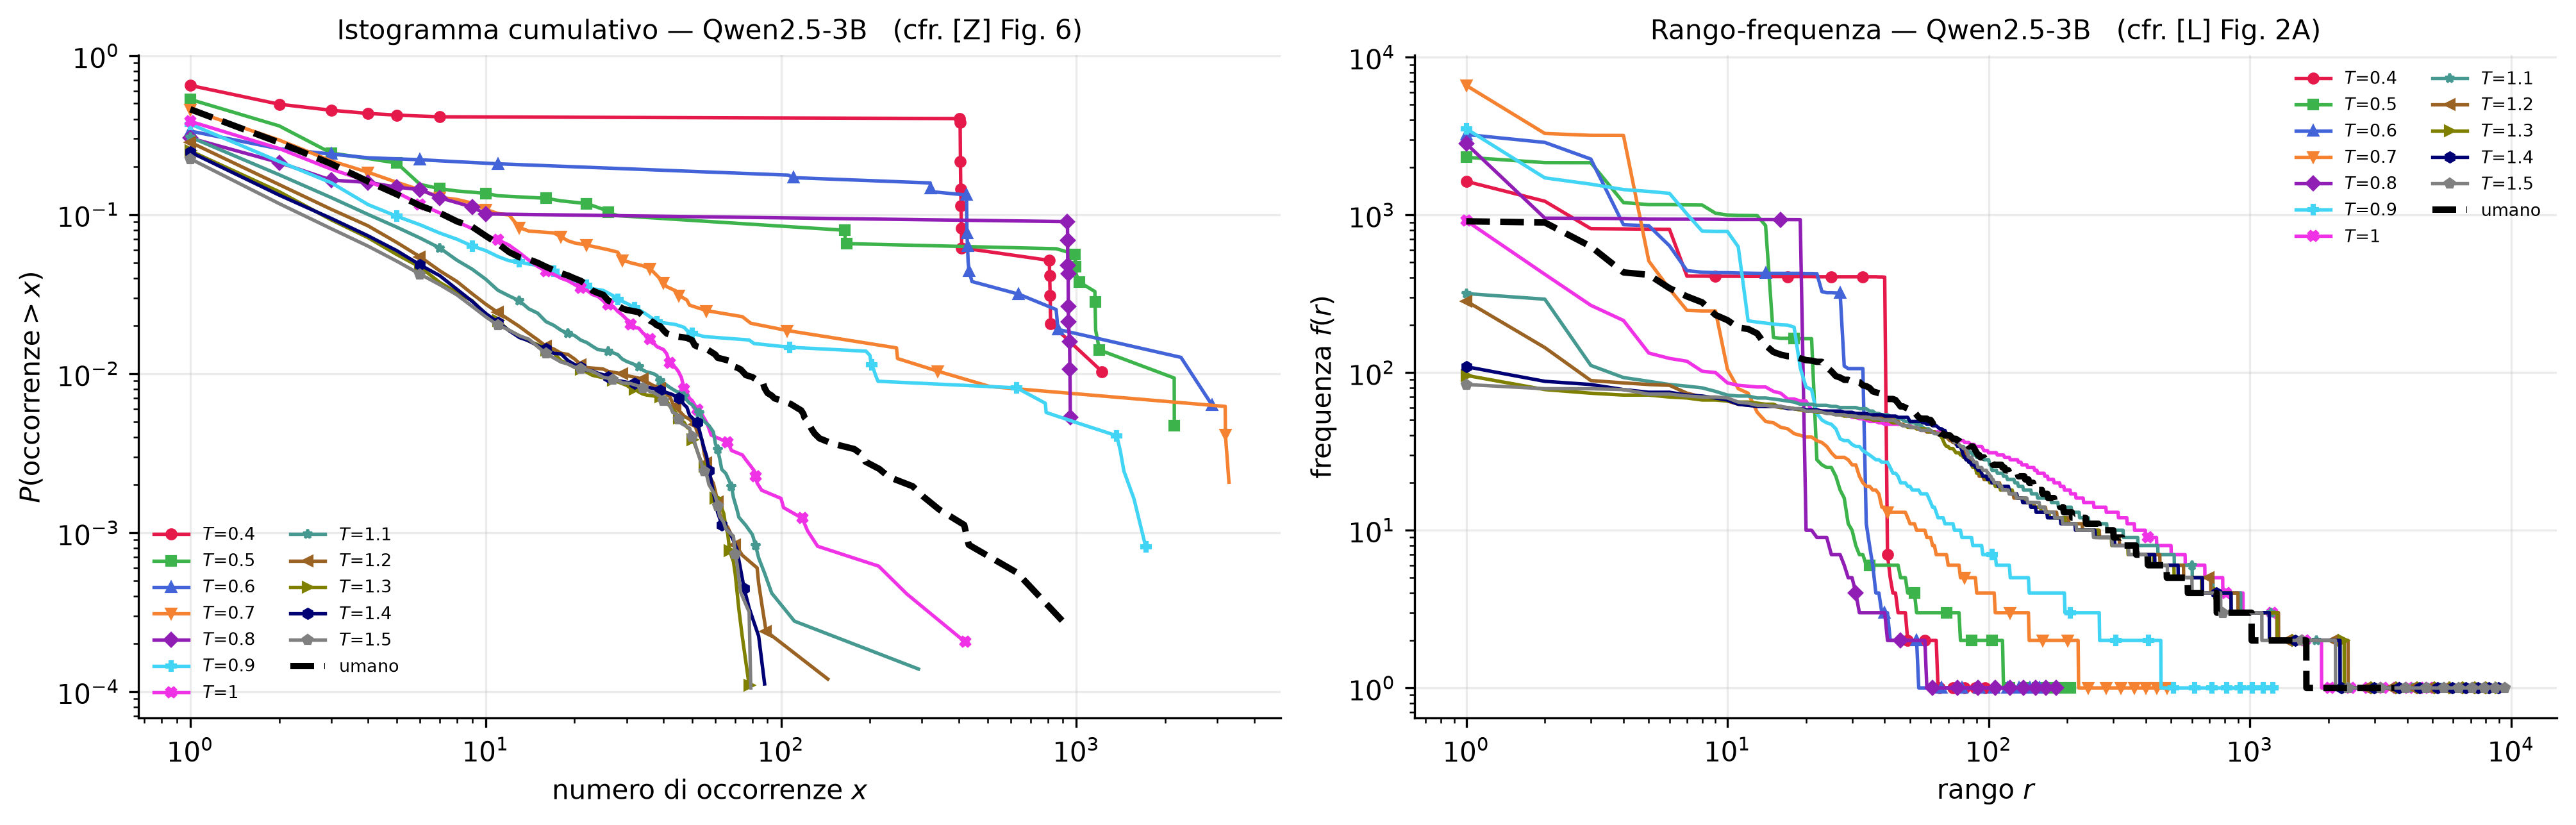
\includegraphics[width=\textwidth]{figure/cap4_zipf_cumulativo_Qwen25_3B.png}
  \caption{Istogrammi cumulativi delle frequenze dei token per il modello
  Qwen2.5-3B, una curva per temperatura. A bassa temperatura la curva è quasi
  verticale, perché pochi token coprono l'intero documento; ad alta temperatura
  è quasi orizzontale, perché quasi ogni token compare una volta sola. Solo
  nella regione intermedia la curva si avvicina alla retta che in coordinate
  bilogaritmiche corrisponde a una legge di potenza.}
  \label{fig:zipf-cum}
\end{figure}

L'esponente da solo non basta a descrivere questo comportamento, ed è la ragione
per cui nel §\ref{sec:zipf} è stato introdotto il MAPE: una curva può avere la
pendenza corretta e una curvatura marcata, e in tal caso l'esponente stimato non
descrive nulla. La Figura~\ref{fig:zipf-vs-T} riporta entrambe le quantità in
funzione della temperatura.

\begin{figure}[htbp]
  \centering
  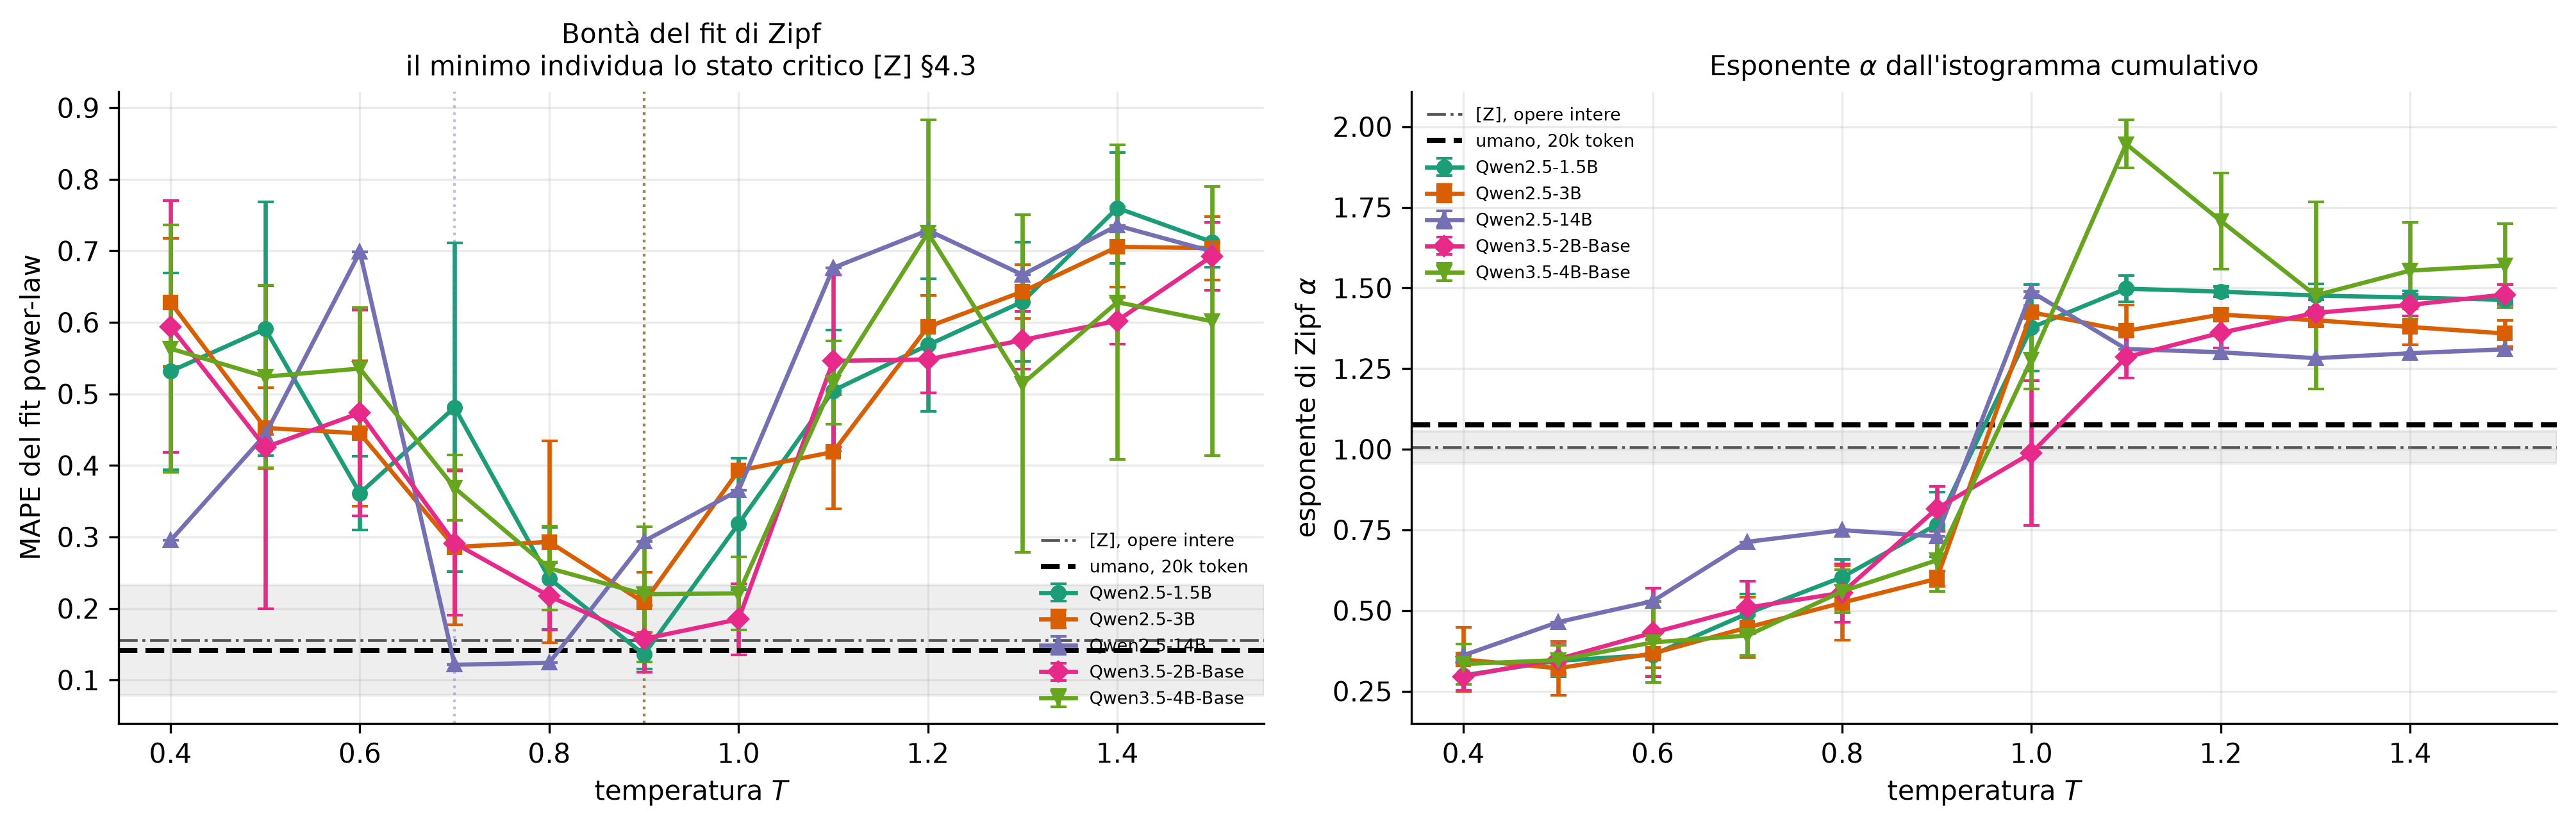
\includegraphics[width=\textwidth]{figure/cap4_zipf_vs_T.png}
  \caption{Bontà del fit e esponente della legge di Zipf in funzione della
  temperatura, per tutti e cinque i modelli. La banda grigia è il valore
  pubblicato su testi letterari interi, la linea nera tratteggiata la baseline
  umana misurata alla lunghezza di lavoro.}
  \label{fig:zipf-vs-T}
\end{figure}

Il MAPE ha un minimo pronunciato, che cade a $T = 0.9$ per quattro modelli su
cinque e a $T = 0.7$ per il modello da 14 miliardi di parametri. È il
risultato centrale della sezione: esiste una temperatura alla quale la
distribuzione delle frequenze del testo generato è più vicina a una legge di
potenza, e ai due lati di essa l'aderenza peggiora rapidamente.

Al minimo il MAPE del modello esemplare vale $0.208$. I due termini di
riferimento sono la baseline umana misurata alla stessa lunghezza, che vale
$0.141$, e il valore $0.156 \pm 0.077$ che~\cite{mikhaylovskiy2025zipf} riporta
su un corpus di sei opere letterarie in cinque lingue. Che i due riferimenti
umani cadano tanto vicini è una verifica indipendente della taratura della
baseline: sono ottenuti con tokenizzatori diversi, su testi diversi e di
lunghezza diversa, e la deriva documentata nella
Figura~\ref{fig:dimensione-finita} non rendeva scontato l'accordo.

Il valore del modello va letto contro tre metri diversi, e il giudizio che se ne
ricava non è lo stesso. Rispetto al modello stesso, $0.208$ è un risultato
netto: alle due estremità dell'intervallo lo stesso modello dà $0.628$ e
$0.704$, cioè un errore di fit tre volte più grande. Rispetto al testo umano è
invece una mezza vittoria: $0.208$ è circa una volta e mezza $0.141$, e resta
dentro la banda pubblicata solo perché quella banda è larga, sfiorandone il
margine superiore $0.233$. Rispetto agli altri modelli, infine, è un risultato
mediocre. La Tabella~\ref{tab:mape-minimi} riporta i cinque minimi: due modelli
scendono sotto il valore umano e un terzo vi si accosta, con $0.158$ contro
$0.141$, mentre il modello esemplare e il Qwen3.5-4B restano sopra.

\begin{table}[htbp]
\centering
\small
\begin{tabular}{@{}lrr@{}}
\toprule
Modello & $T$ del minimo & MAPE al minimo \\
\midrule
Qwen2.5-14B      & 0.7 & 0.121 \\
Qwen2.5-1.5B     & 0.9 & 0.136 \\
Qwen3.5-2B-Base  & 0.9 & 0.158 \\
Qwen2.5-3B       & 0.9 & 0.208 \\
Qwen3.5-4B-Base  & 0.9 & 0.220 \\
\midrule
testo umano      & --- & 0.141 \\
\bottomrule
\end{tabular}
\caption{Valore minimo del MAPE e temperatura alla quale viene raggiunto, per
ciascun modello, con la baseline umana misurata alla stessa lunghezza. Il
minimo esiste per tutti e cinque, ma solo tre modelli lo portano al livello del
testo umano o sotto. La riga del Qwen2.5-14B è ricavata da un solo campione per
temperatura e va letta con la cautela discussa nel testo.}
\label{tab:mape-minimi}
\end{table}

La prima riga della tabella richiede una precauzione. Il Qwen2.5-14B è l'unico
modello con un solo campione per temperatura, contro i tre o cinque degli altri,
e la sua curva del MAPE non è regolare da nessuno dei due lati del minimo: vale
$0.295$ a $T = 0.4$, sale a $0.698$ a $T = 0.6$ e scende a $0.121$ a $T = 0.7$,
cioè peggiora di un fattore due e migliora di un fattore sei in due passi
consecutivi. Negli altri quattro modelli la dispersione fra campioni alla stessa
temperatura va da $0.046$ a $0.230$ attorno a $T = 0.7$, mentre la distanza fra
il minimo del 14B e il suo valore a $T = 0.9$ vale $0.173$: sta dentro
quell'intervallo. Con una sola realizzazione la posizione del minimo non è
risolvibile, e il valore $T = 0.7$ va letto come compatibile con il $T = 0.9$
degli altri quattro anziché come uno spostamento reale. La stessa cautela vale
per la profondità: $0.121$ è il minimo più basso dei cinque ed è anche il meno
affidabile, mentre il $0.136$ del Qwen2.5-1.5B poggia su cinque campioni con
dispersione $0.020$ ed è l'unico caso in cui il primato sul testo umano è
sostenuto da repliche.

La posizione del minimo va confrontata con quella riportata nella fonte.
In~\cite{mikhaylovskiy2025zipf} il minimo del MAPE cade fra $t = 1.0$ e
$t = 1.2$ per tutti i modelli tranne i Llama più grandi, mentre qui cade a
$T = 0.9$ per quattro modelli su cinque. Lo scarto è nella direzione prevista
dall'effetto del prompt descritto nel §\ref{sec:protocollo}, che abbassa
l'errore del fit soprattutto alle basse temperature e sposta quindi il minimo
verso sinistra.

Ne segue una distinzione che vale per tutto il seguito. L'esistenza
di una temperatura ottimale è un fatto generale, comune a tutti e cinque i
modelli; la qualità dell'ottimo, cioè quanto il testo generato in quel punto
somigli davvero a un testo umano, varia da modello a modello e non è garantita.
Il modello scelto come esemplare non è fra quelli che ci riescono, e i grafici
del corpo del capitolo vanno letti tenendolo presente.

L'esponente $\alpha$ racconta la stessa storia da un'altra angolazione. Per il
modello esemplare passa da $0.35$ a $T = 0.4$, valore che corrisponde a una
distribuzione dominata da pochissimi tipi, a $1.36$ a $T = 1.5$, dove più di tre
quarti dei tipi compaiono una volta sola.\footnote{Un tipo che compare una sola
volta nel testo si dice \emph{hapax}. Gli hapax sono normalmente la maggioranza
dei tipi ma una piccola parte delle occorrenze: nella baseline umana usata qui
sono il $54\%$ dei tipi e il $10\%$ dei token, mentre a $T = 1.5$ il modello
esemplare arriva al $77\%$ dei tipi e al $37\%$ dei token.} La transizione non è
graduale: fra $T = 0.9$ e $T = 1.0$ l'esponente salta da $0.60$ a $1.43$,
attraversando in un solo passo il valore umano $1.076$, per poi assestarsi
attorno a $1.4$ senza più avvicinarvisi.

% ---------------------------------------------------------------------
\section{Legge di Heaps e descrittore \texorpdfstring{$R$}{R}}
\label{sec:heaps-risultati}

Le curve di crescita del vocabolario rendono immediatamente evidente perché il
§\ref{sec:heaps} abbia dovuto introdurre un descrittore alternativo all'esponente di
Heaps.

\begin{figure}[htbp]
  \centering
  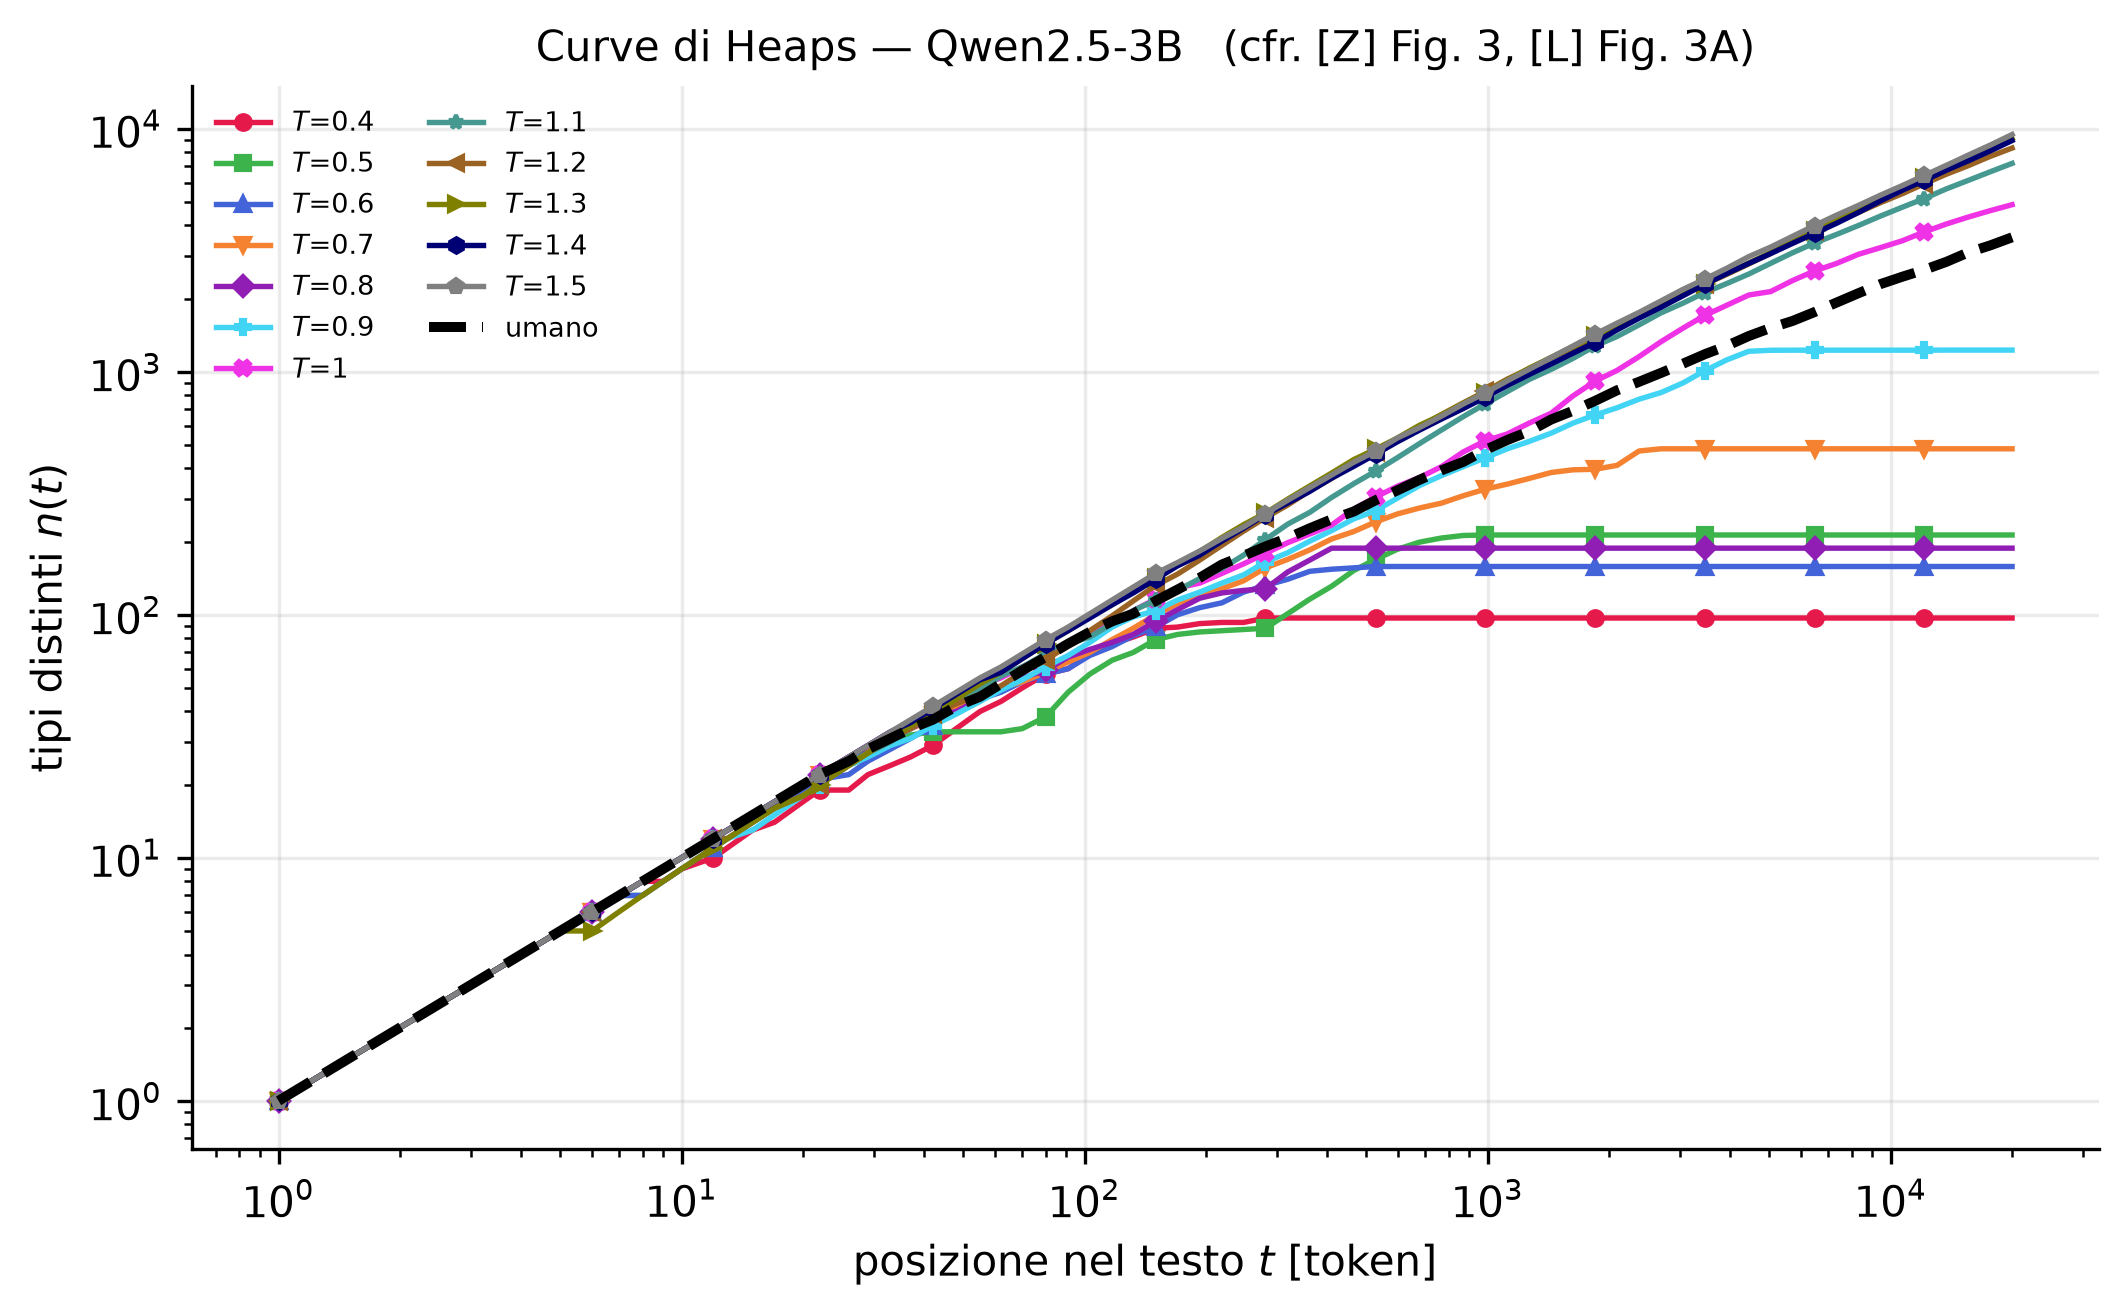
\includegraphics[width=0.86\textwidth]{figure/cap4_heaps_curve_Qwen25_3B.png}
  \caption{Crescita del vocabolario per il modello Qwen2.5-3B. Alle temperature
  basse la curva si appiattisce dopo poche migliaia di token: il modello ha
  smesso di produrre tipi nuovi. Alle temperature alte cresce quasi linearmente.
  In nessuno dei due casi la curva è una legge di potenza, e stimarne
  l'esponente restituisce un numero privo di contenuto.}
  \label{fig:heaps-curve}
\end{figure}

La Figura~\ref{fig:heaps-R} riporta il descrittore $R$, l'esponente $\gamma_H$
e il rapporto fra tipi e occorrenze in funzione della temperatura. I tre
andamenti sono concordi: per il modello esemplare $\gamma_H$ passa da $0.001$
a $T = 0.4$, dove la curva è piatta e il vocabolario non cresce affatto, a
$0.806$ a $T = 1.5$, attraversando il valore umano $0.668$ poco sopra $T =
0.9$. Il descrittore $R$ passa da $0.003$ a $0.688$ e incrocia il valore umano
$0.507$ attorno a $T = 1.05$.

Il terzo pannello riporta la quantità più elementare delle tre, il rapporto fra
il numero di tipi distinti e il numero di occorrenze, e serve da controllo sulle
altre due. A differenza di $\gamma_H$ e di $R$ non richiede alcun fit né alcuna
partizione del documento, quindi non può essere alterato da un modello mal
specificato: se le tre curve concordano, l'andamento non è un artefatto della
procedura di stima. Per il modello esemplare passa da $0.007$ a $T = 0.4$ a
$0.474$ a $T = 1.5$, e attraversa il valore umano $0.179$ fra $T = 0.9$ e
$T = 1.0$, cioè nello stesso punto delle altre due misure. Il pannello mostra
però anche in che senso l'accordo con il testo umano sia solo locale: sopra
$T = 1.1$ il rapporto supera il doppio del valore umano e continua a crescere,
mentre $\gamma_H$ resta stabile attorno a $0.8$. Le due misure smettono di dire
la stessa cosa non appena il vocabolario si allarga oltre quello di un romanzo.

\begin{figure}[htbp]
  \centering
  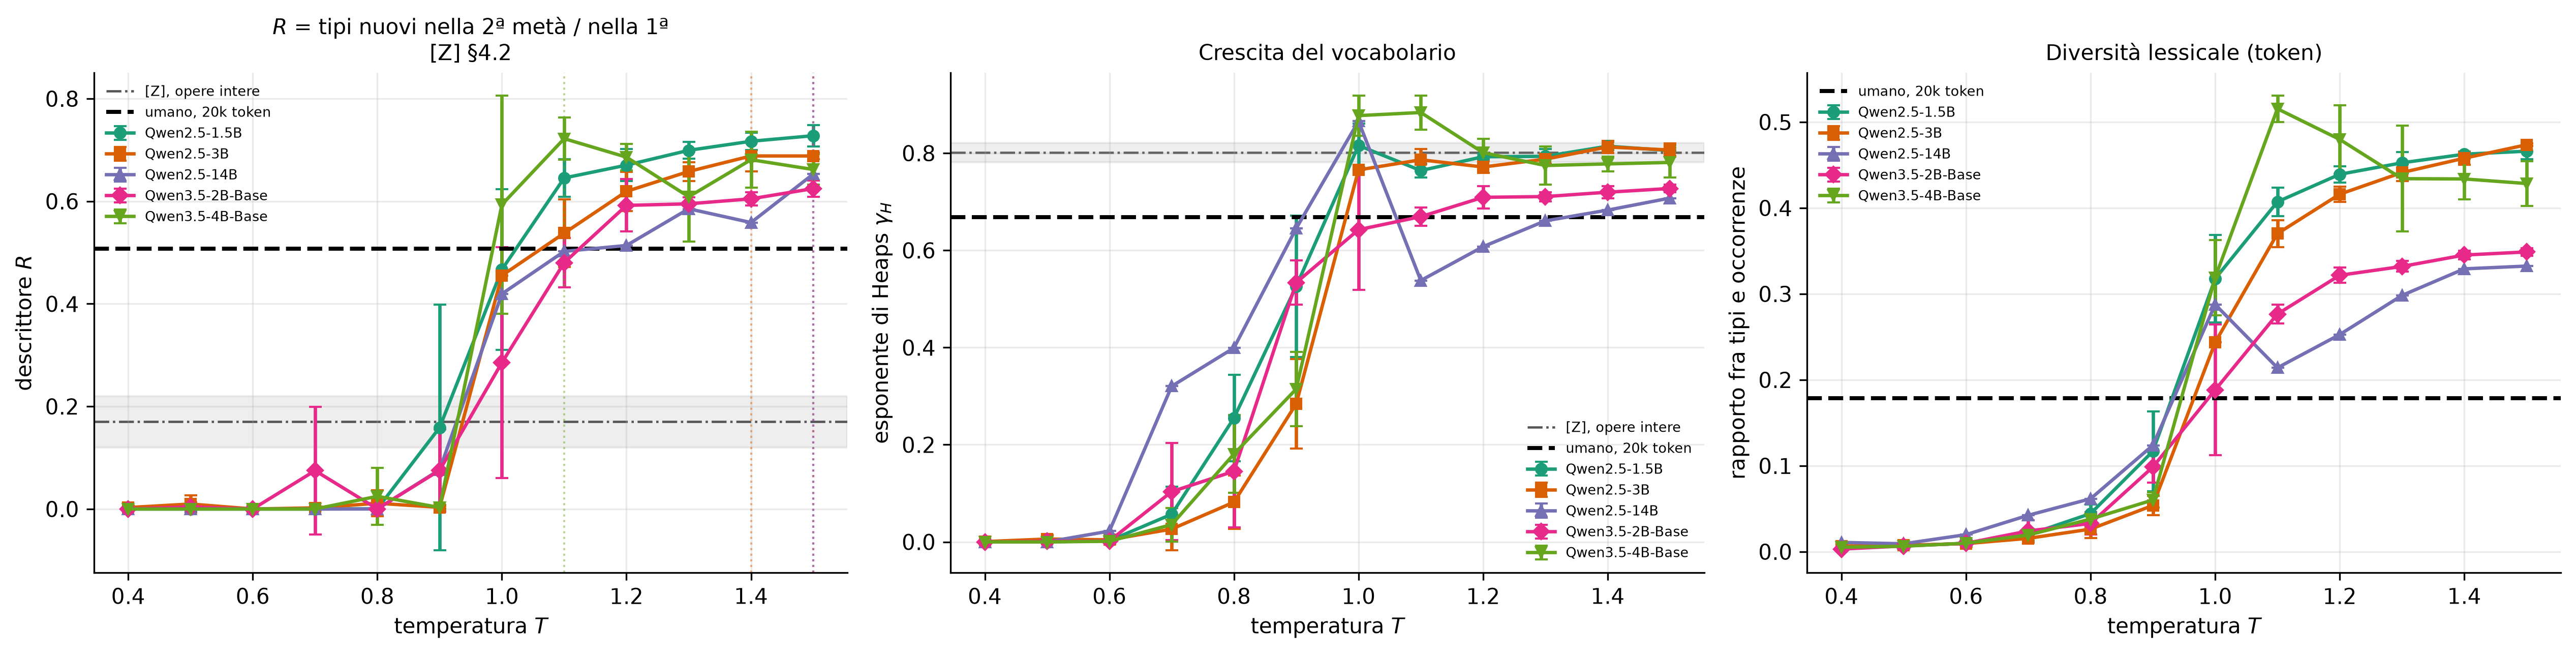
\includegraphics[width=\textwidth]{figure/cap4_heaps_R_vs_T.png}
  \caption{Descrittore $R$, esponente di Heaps e rapporto fra tipi e occorrenze
  in funzione della temperatura. La banda grigia riporta i valori pubblicati su
  opere intere, che per le ragioni discusse nel §\ref{sec:scelte} non sono un
  termine di confronto diretto.}
  \label{fig:heaps-R}
\end{figure}

% ---------------------------------------------------------------------
\section{Correlazioni a lungo raggio}
\label{sec:dfa-risultati}

Ogni documento viene convertito nella successione numerica definita nel
§\ref{sec:dfa}: ogni carattere è sostituito dal proprio rango di frequenza nel
documento, $1$ al più frequente, $2$ al secondo, e così via. È su quella
successione che si misura l'esponente della fluttuazione. Il detrending è
quadratico: il §\ref{sec:robustezza} documenta il confronto con quello lineare e
la ragione della scelta, cioè che alle basse temperature i documenti non sono
stazionari e un polinomio di primo grado non assorbe la deriva della
composizione dei caratteri. Il primo controllo riguarda il null model: la stessa
analisi condotta sui documenti rimescolati deve restituire un esponente pari a
$1/2$.


La Figura~\ref{fig:dfa} riporta le curve di fluttuazione e l'esponente in
funzione della temperatura. L'esponente ha un massimo a $T = 1.0$, dove vale
$0.719$ in media su tutti i modelli, superiore al valore umano di $0.579$;
decresce poi verso $0.53$ alle temperature più alte, avvicinandosi al valore del
rimescolamento senza raggiungerlo.

\begin{figure}[htbp]
  \centering
  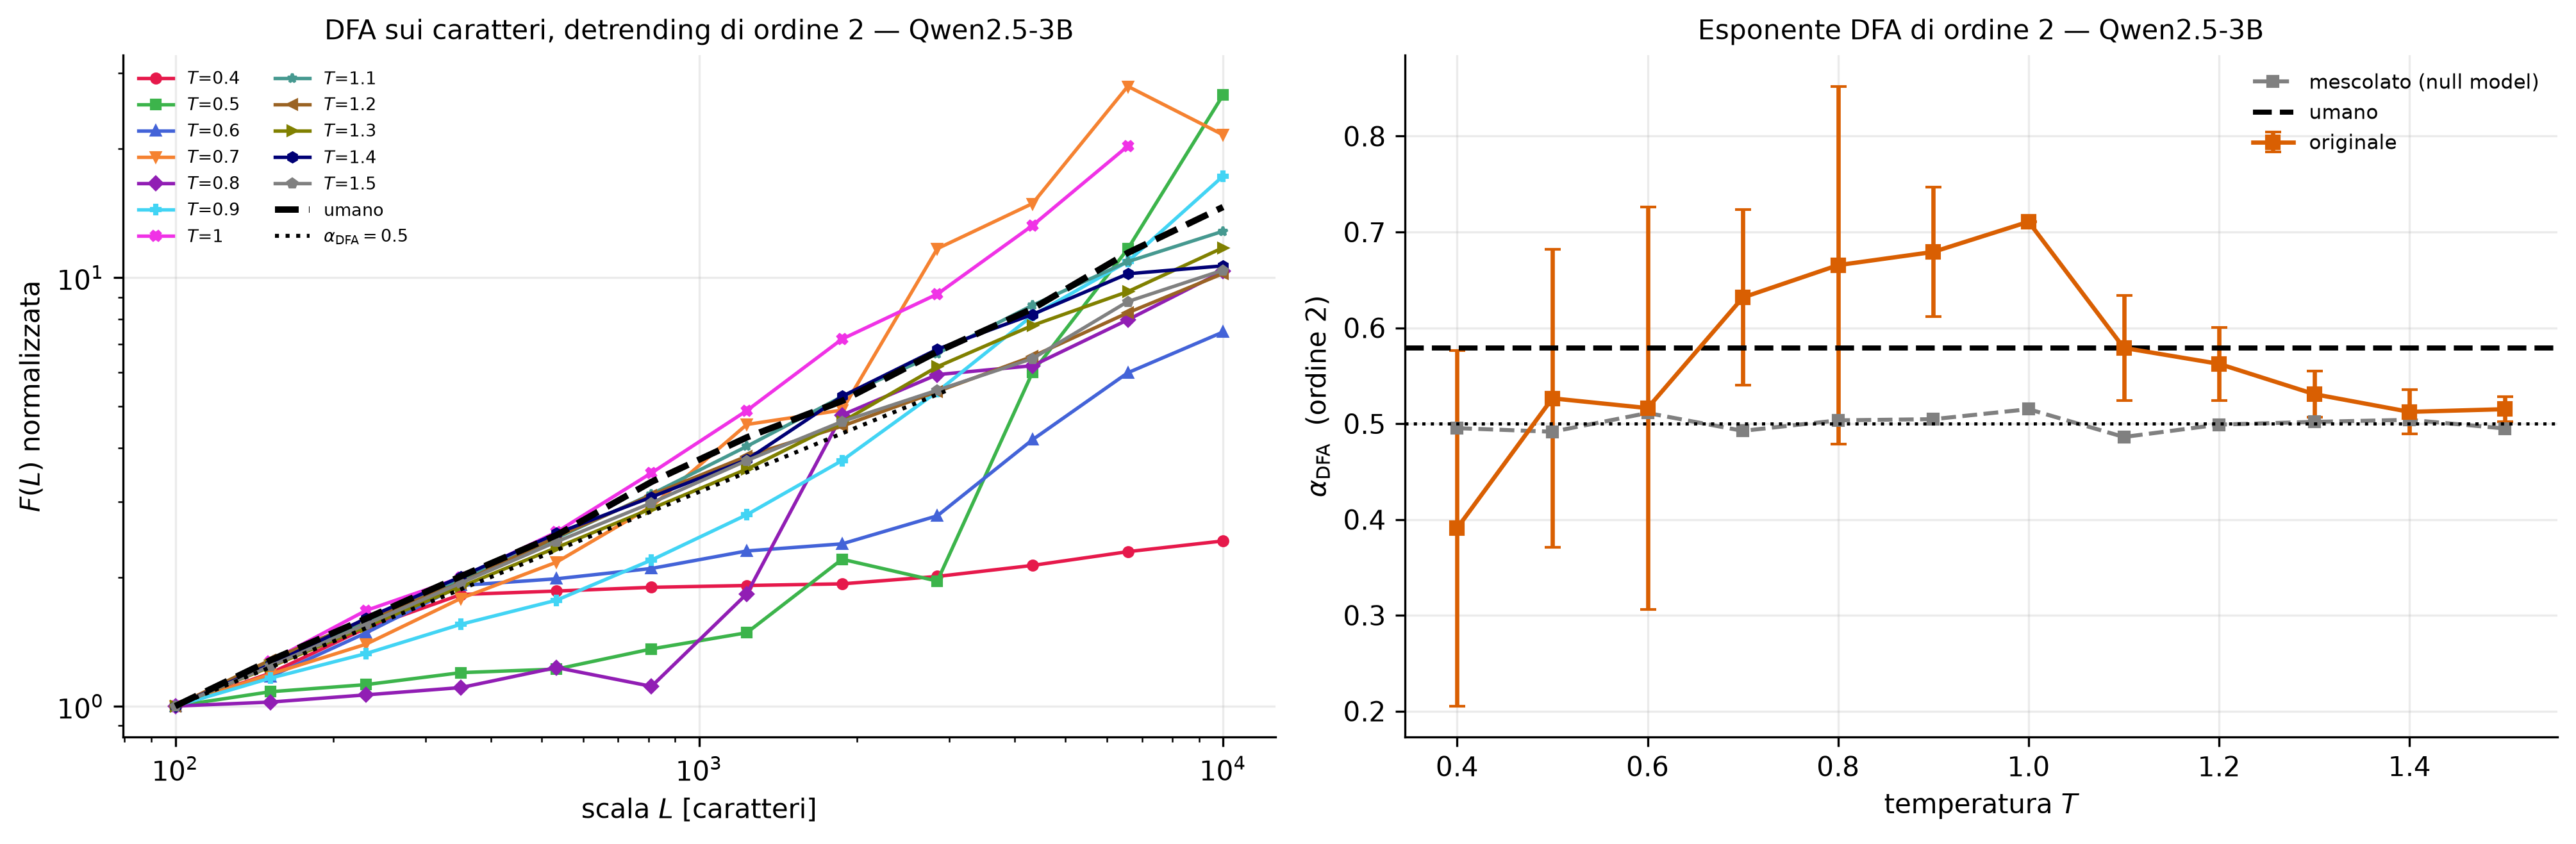
\includegraphics[width=\textwidth]{figure/cap4_dfa_Qwen25_3B_o2.png}
  \caption{Fluttuazione detrendizzata per il modello Qwen2.5-3B, con detrending
  quadratico. A sinistra $F(s)$ in funzione della scala, una curva per
  temperatura, con la pendenza di riferimento $\alpha_{\mathrm{DFA}} = 1/2$; a
  destra l'esponente in funzione della temperatura, con il null model
  rimescolato e la baseline umana.}
  \label{fig:dfa}
\end{figure}

\paragraph{La dispersione è il vero segnale.}
Il valore medio dell'esponente nasconde il fenomeno più informativo, ed è un
fenomeno già osservato: sulle reti LSTM~\cite{lippi2019} riporta che le stime
sui singoli campioni sono molto disperse attorno a $T = 0.5$ e strettamente
raccolte attorno alla media a $T = 1.0$. Gli stessi dati mostrano qui lo stesso
comportamento su architetture transformer. La deviazione standard fra documenti
passa da $0.219$ a $T = 0.4$ a $0.022$ a $T = 1.4$: alle basse temperature la
stima è dieci volte più dispersa. A $T = 0.4$ i cinque documenti del modello
esemplare danno esponenti compresi fra $0.16$ e $0.66$, cioè coprono
l'intervallo fra la saturazione e il valore umano; sull'insieme dei cinque
modelli l'escursione va da $0.07$ a $0.89$.

Questo comportamento è coerente con il caso limite discusso nel
§\ref{sec:ponte}. Quando il testo entra in un ciclo di ripetizione, il profilo
cumulato oscilla invece di allontanarsi dall'origine e la fluttuazione satura:
l'esponente crolla. Il crollo dipende però dalla lunghezza del ciclo rispetto
alle scale analizzate, che varia da documento a documento, e non tutti i testi
ripetitivi lo manifestano.

I dati permettono di precisare la relazione, che è a senso unico. Tutti e
diciannove i documenti con $\alpha_{\mathrm{DFA}} < 0.3$ si trovano a
$T \le 0.6$ e hanno una quota media di 8-grammi ripetuti pari a $0.984$: un
esponente collassato implica dunque ripetizione conclamata. Il viceversa non
vale: fra gli 82 documenti con quota di 8-grammi ripetuti superiore a $0.9$,
soltanto 33 hanno un esponente inferiore a $1/2$, e la correlazione di rango fra
le due quantità non è significativa
($\rho = +0.03$, $p = 0.61$). La ripetizione è quindi condizione necessaria ma
non sufficiente al collasso dell'esponente.

Ne segue una conseguenza metodologica. Alle basse temperature
$\alpha_{\mathrm{DFA}}$ non è un indicatore affidabile di correlazione a lungo
raggio, né lo è il suo valore medio; è la sua dispersione a segnalare il regime.
Il controllo sull'ordine del detrending riportato nel §\ref{sec:robustezza}
punta nella stessa direzione, poiché lo scarto fra i due ordini è massimo
proprio nell'intervallo $T \in [0.5, 0.8]$ e trascurabile altrove.

% ---------------------------------------------------------------------
\section{Entropia, divergenza dal testo umano e plagio}
\label{sec:entropia-risultati}

Le sezioni precedenti confrontano il testo generato con quello umano una misura
alla volta. La divergenza di Kullback--Leibler introdotta nel
§\ref{sec:crossparsing} permette invece un confronto diretto fra i due testi,
senza passare per un descrittore intermedio, ed è per questa ragione il criterio
più stringente del capitolo: non dipende da soglie teoriche né dalla scelta di
quale proprietà misurare.


La divergenza ha un minimo netto, che cade a $T = 0.9$ per quattro modelli su
cinque e a $T = 1.0$ per Qwen3.5-4B-Base. Nessuna delle \num{242} stime risulta
negativa, il che conferma sui dati reali la proprietà dello stimatore verificata
nel §\ref{sec:validazione}.

Il valore al minimo varia molto fra i modelli: $0.096$ bit per carattere per il
modello da 14 miliardi di parametri, $0.232$ e $0.245$ per i due Qwen3.5,
$0.321$ per il modello da 1.5 miliardi e $0.914$ per quello da 3 miliardi. La
posizione del minimo è dunque comune, la sua profondità no: fra il modello che
si avvicina di più al testo umano e quello che ci riesce meno corre quasi un
fattore dieci. La profondità non segue però la dimensione. La correlazione di
rango con il numero di parametri vale $\rho = -0.50$ con $p = 0.39$ su cinque
modelli, e il valore peggiore appartiene al modello da 3 miliardi anziché al più
piccolo: quanto un modello si avvicini al testo umano nel proprio punto migliore
è una proprietà del singolo modello, non della sua scala, almeno con la potenza
statistica qui disponibile. Vale inoltre la cautela imposta dal
§\ref{sec:robustezza}, poiché il modello da 14 miliardi dispone di un solo
campione per temperatura e il suo valore non è corredato da una stima della
dispersione.

L'entropia stimata per compressione mostra la transizione in modo ancora più
brusco. Per il modello esemplare la mediana vale $0.001$ bit per carattere
fino a $T = 0.8$, perché il testo ripetitivo è essenzialmente incomprimibile
oltre la prima occorrenza del ciclo e non trasporta informazione; sale poi a
$0.332$ in media a $T = 0.9$ e supera $4$ da $T = 1.0$ in poi, contro i $2.23$
del testo umano. Fra $T = 0.6$ e $T = 0.9$ la media si stacca dalla mediana
perché un documento per temperatura esce dal ciclo prima degli altri, e il
valore isolato di $5.77$ che il modello esemplare raggiunge a $T = 1.0$
proviene dall'unico documento sopravvissuto a quella temperatura: è la stessa
dispersione descritta nel §\ref{sec:dfa-risultati}, e conferma che nel regime
periodico il valore medio non descrive alcun documento. Il passaggio dal
regime a entropia trascurabile a quello a entropia superiore a quella umana si
consuma comunque entro due passi di temperatura.

% ---------------------------------------------------------------------
\section{Struttura misurata per compressione}
\label{sec:compressione-risultati}

Le misure basate su compressione del §\ref{sec:compressione} non richiedono di
scegliere un'unità di analisi né di stimare un esponente: operano direttamente
sui byte del testo. Costituiscono quindi un controllo indipendente da tutte le
scelte metodologiche discusse finora.

\begin{figure}[htbp]
  \centering
  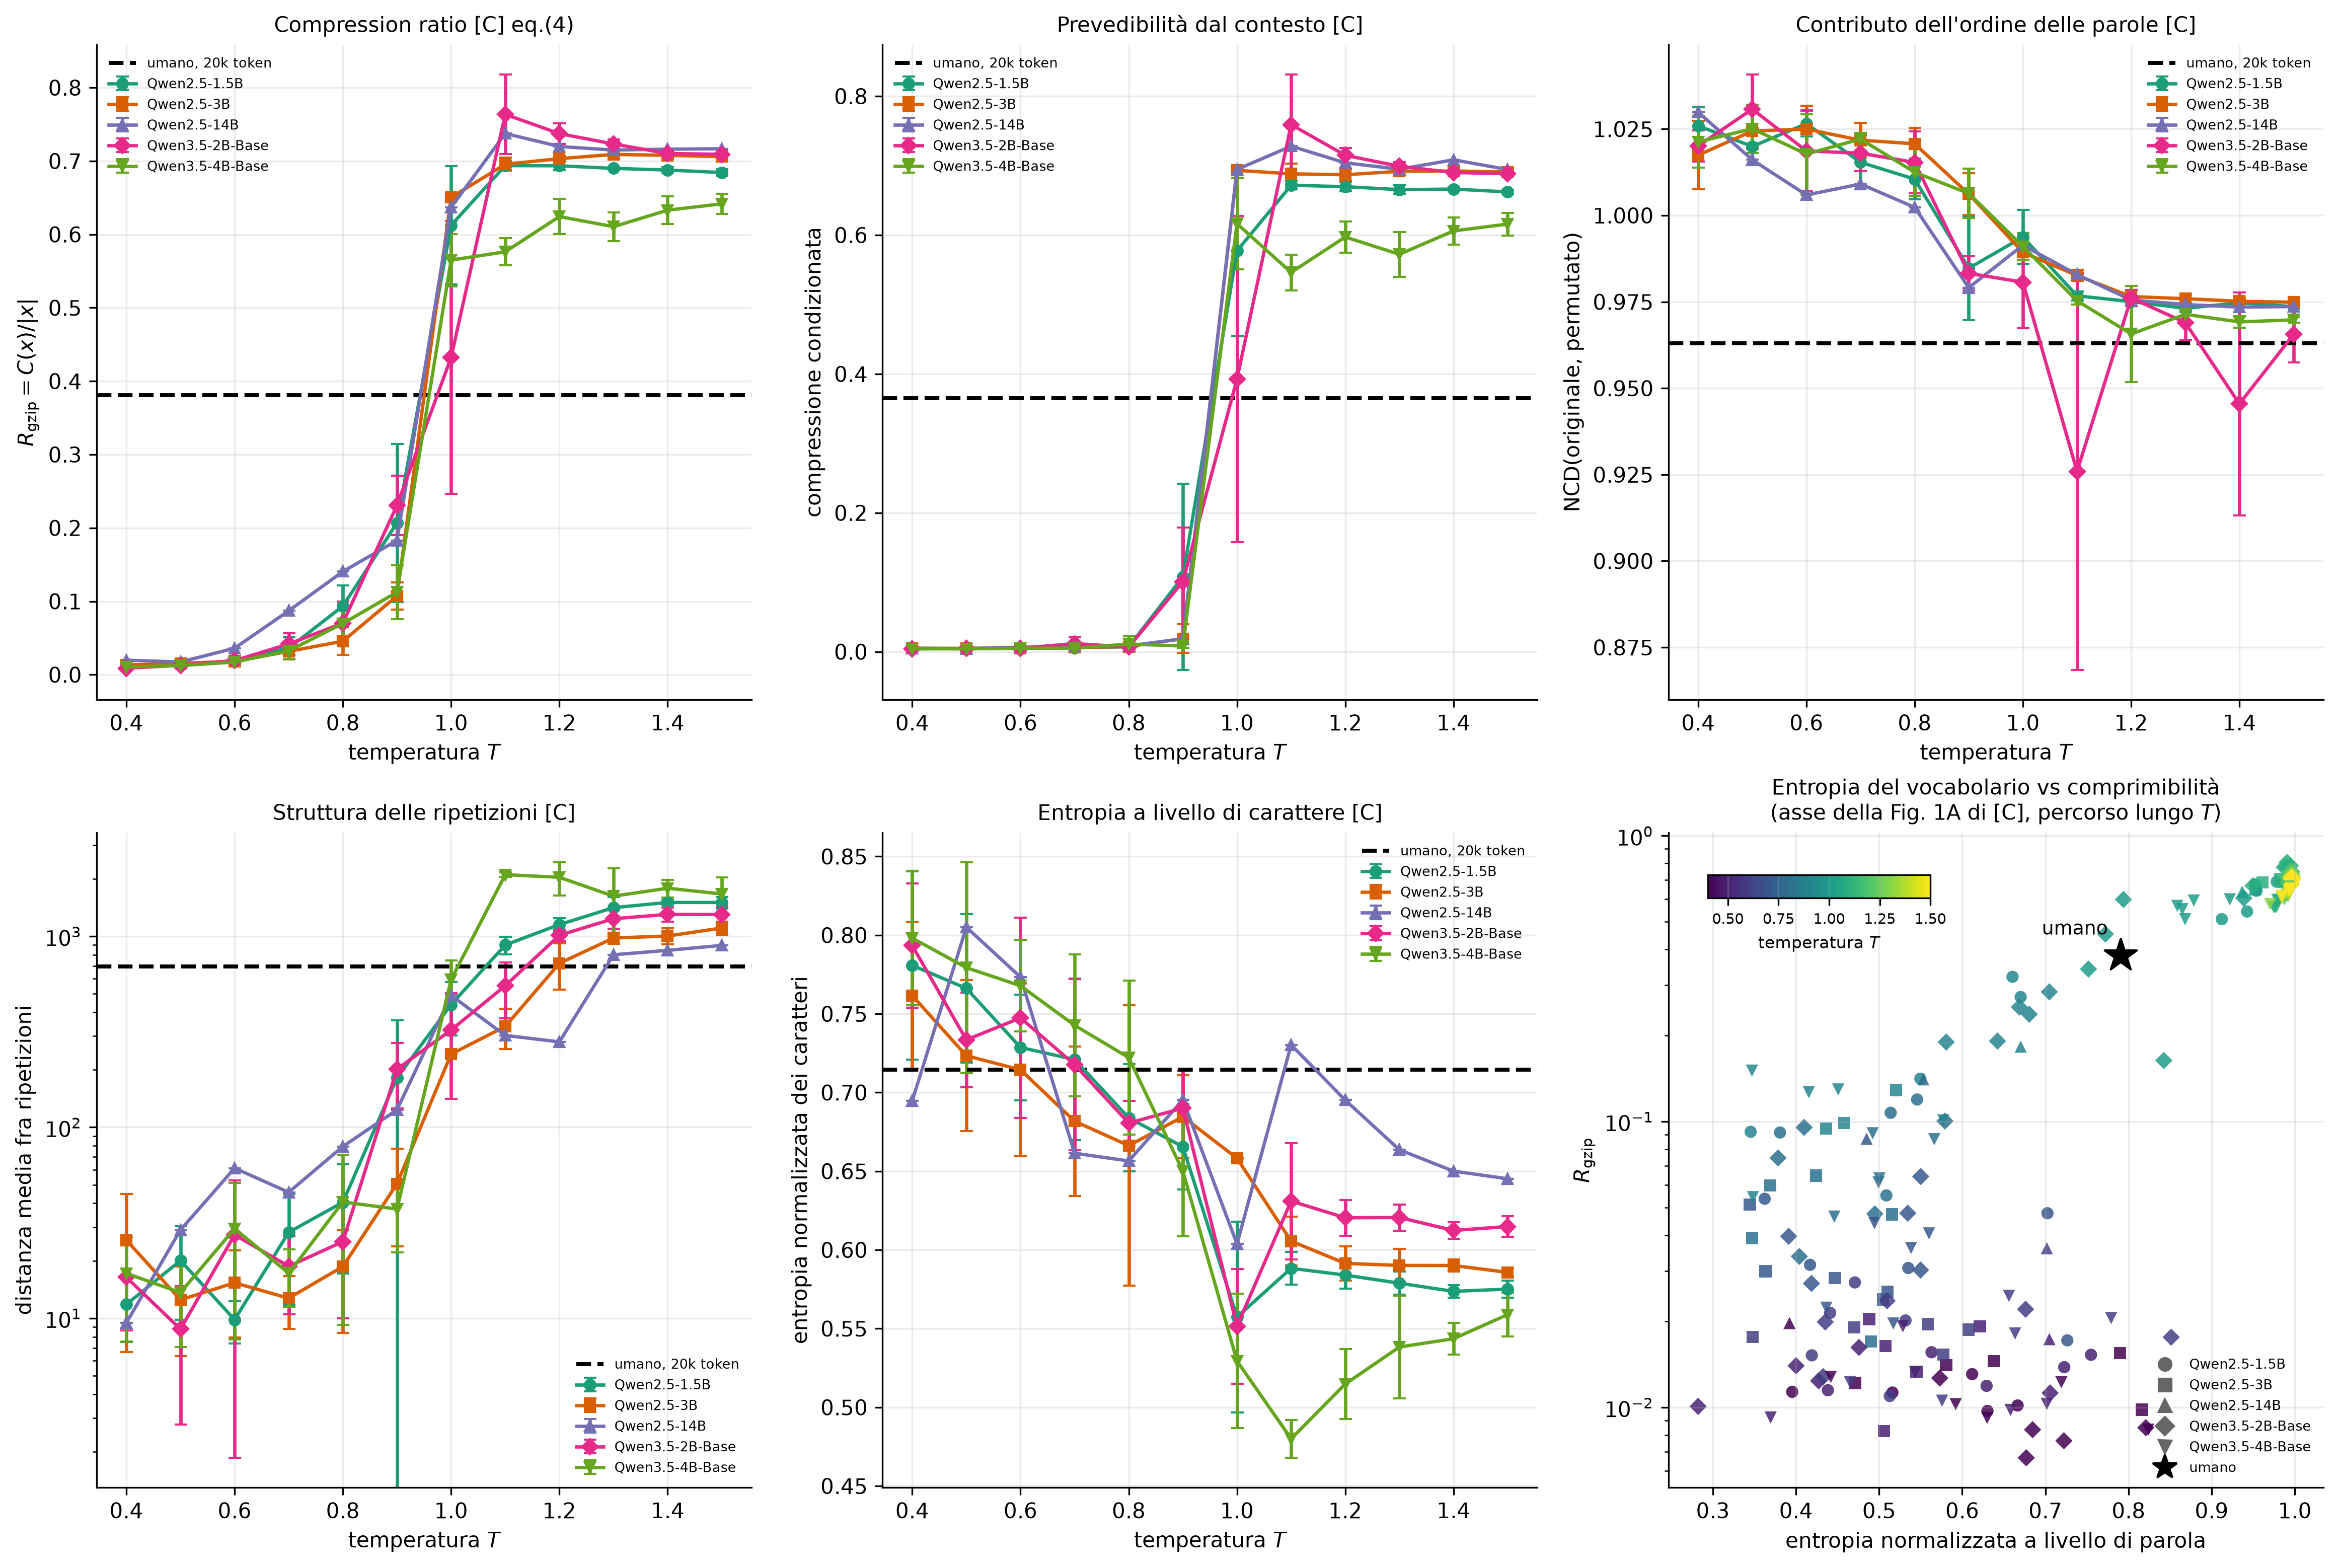
\includegraphics[width=\textwidth]{figure/cap4_compressione.png}
  \caption{Sei misure basate su compressione. Le prime cinque sono riportate in
  funzione della temperatura; l'ultima, in basso a destra, riporta il rapporto
  di compressione contro
  l'entropia normalizzata a livello di parola: è il piano della Figura~1A
  di~\cite{hadad2026}, percorso qui facendo variare la temperatura, con il testo
  umano segnato da una stella. In quel pannello il colore codifica la
  temperatura e la forma del marcatore il modello, e la scala verticale è
  logaritmica.}
  \label{fig:compressione}
\end{figure}

Il rapporto di compressione è la misura che separa i regimi in modo più netto di
tutte le altre. Per il modello esemplare passa da $0.013$ a $T = 0.4$ a $0.107$
a $T = 0.9$ e a $0.650$ a $T = 1.0$: un fattore cinquanta fra i due estremi, con
un salto di un fattore sei concentrato in un singolo passo di temperatura. Il
valore umano è $0.381$, e viene attraversato fra $T = 0.9$ e $T = 1.0$ come
tutte le altre misure del capitolo.

Il lavoro di~\cite{hadad2026} riporta che il testo generato è più regolare e
più comprimibile di quello umano, mentre qui il rapporto di compressione
supera il valore umano sopra $T = 1.0$. Le due osservazioni non sono in
contrasto, perché descrivono regioni diverse dello stesso asse: sotto la
transizione il testo generato è molto più comprimibile del testo umano,
$0.013$ contro $0.381$, ed è il regime in cui i modelli operano con le
impostazioni ordinarie; sopra la transizione la comprimibilità cade perché il
testo cessa di essere linguaggio, non perché acquisti struttura.

La compressione condizionata si comporta in modo analogo ma dice qualcosa di
diverso. Fino a $T = 0.9$ vale meno di $0.02$: la seconda metà del documento è
quasi interamente prevedibile dalla prima, come è ovvio in un testo che ripete
lo stesso ciclo. Da $T = 1.0$ sale a circa $0.69$, quasi il doppio del valore
umano $0.365$: la seconda metà è ora \emph{meno} prevedibile dalla prima di
quanto lo sia in un romanzo. Fra i due regimi non esiste una temperatura in cui
la predicibilità dal contesto assomigli a quella del testo umano.

Il salto oltre il valore umano non è una particolarità del modello esemplare. La
mediana su tutti e cinque i modelli passa da $0.015$ a $T = 0.9$ a $0.627$ a
$T = 1.0$, e il singolo modello che si avvicina di più al valore umano da sotto,
il Qwen3.5-2B-Base con $0.135$, lo scavalca comunque in un passo arrivando a
$0.430$. Nessuno dei cinque si ferma sul valore umano, ed è l'unica delle misure
di questo capitolo per cui ciò accade.

\paragraph{Il piano entropia--comprimibilità.}
Il pannello in basso a destra della Figura~\ref{fig:compressione} colloca i
documenti nel piano definito da~\cite{hadad2026}, percorso qui da un modello
reale al variare di un solo parametro anziché da distribuzioni artificiali, con
il testo umano in posizione intermedia. L'asse verticale è logaritmico perché il rapporto di compressione
non si annulla mai: il valore più basso osservato è $0.0067$. Su un asse
lineare esteso fino a $0.81$, però, i 57 documenti che stanno fra $0.007$ e
$0.020$, quasi un quarto del totale, si sovrappongono tutti sulla linea dello
zero, e la loro struttura interna scompare. In scala logaritmica si vede
invece che occupano un intervallo di entropia molto ampio, da $0.28$ a $0.85$,
e la ragione è che le due grandezze misurano cose diverse. Il rapporto di
compressione dipende dalla ripetizione della sequenza: un testo che ripete
sempre lo stesso ciclo si comprime a poco più dell'un per cento della sua
dimensione, qualunque sia il numero di parole che il ciclo contiene.
L'entropia normalizzata dipende invece dalla forma della distribuzione delle
frequenze su quel vocabolario ridotto, che conta fra 37 e 235 tipi distinti.
Un ciclo lungo e vario e un ciclo corto e povero sono ugualmente comprimibili
ma hanno entropie molto diverse: da qui la dispersione orizzontale della
nuvola a bassa comprimibilità.

\paragraph{La lunghezza del ciclo, misurata.}
L'argomento appena esposto invoca una grandezza che le misure di questo capitolo
non contengono, la lunghezza del ciclo ripetuto, ed è quindi il caso di
misurarla. Sulla successione di parole di ciascun documento si cerca il più
piccolo sfasamento $L_{\mathrm{ciclo}}$ per cui l'accordo fra la parola in
posizione $i$ e quella in posizione $i - L_{\mathrm{ciclo}}$, calcolato sugli
ultimi venti giri, supera il novanta per cento. La finestra di verifica è locale
e commisurata al periodo candidato: su tutto il testo la prosa che precede il
ciclo diluirebbe la media, mentre su un suffisso lungo un ciclo che cambia
lentamente variante scende sotto soglia al proprio periodo e la supera a un
multiplo, restituendo un alias. La soglia è fissata al novanta e non al cento
per cento per tollerare i cicli non esattamente verbatim; l'accordo atteso per
caso in prosa inglese è circa $0.05$, quindi non vi sono falsi positivi.

Il criterio individua \num{113} documenti su \num{242}, e sono tutti a
$T \le 0.9$: la totalità fino a $T = 0.7$, il $95\%$ a $T = 0.8$, il $56\%$ a
$T = 0.9$ e nessuno da
$T = 1.0$ in poi. Coincidono con la nuvola a bassa comprimibilità: tutti e
cinquantasette i documenti con $R_{\mathrm{gzip}} < 0.02$ sono fra questi. Il
ciclo va da una sola parola a \num{248}, in caratteri da $9$ a \num{1127}, con
mediana di $16$ parole.

La Figura~\ref{fig:ciclo} riporta la relazione con le due grandezze del piano.
Con l'entropia di parola la correlazione di rango vale $\rho = +0.65$, e non è
un effetto della temperatura: calcolata fra documenti generati alla stessa
temperatura sale a $+0.69$, ed è positiva in tutti e sei i gruppi. Con il
rapporto di compressione, invece, non c'è relazione: $\rho = -0.15$ con
$p = 0.12$, e a temperatura fissata il segno si inverte, $+0.16$ con
$p = 0.11$. A parità di lunghezza del ciclo il rapporto di compressione varia di
un fattore compreso fra quattordici e ventisette.

Il meccanismo è quello anticipato sopra, e la misura lo rende esplicito: la
lunghezza del ciclo coincide quasi con il numero di tipi distinti che esso
contiene, $\rho = +0.84$, cosicché un ciclo corto concentra tutta la massa di
probabilità su poche parole e uno lungo la distribuisce. Gli estremi lo
mostrano nel modo più diretto: il ciclo più corto osservato è una sola parola,
ripetuta, con entropia $0.35$; il più lungo conta \num{248} parole e undici
tipi distinti, \emph{You are a bad father. You are a bad lover of children.
You are not to blame} con variazioni, con entropia $0.47$ e $R_{\mathrm{gzip}}
= 0.019$, cioè testo ancora ultracomprimibile. La lunghezza del ciclo spiega
dunque l'ordinamento lungo l'asse orizzontale del piano, non tutta la sua
dispersione: la regressione su $\log L_{\mathrm{ciclo}}$ rende conto del
$42\%$ della varianza dell'entropia.

\begin{figure}[htbp]
  \centering
  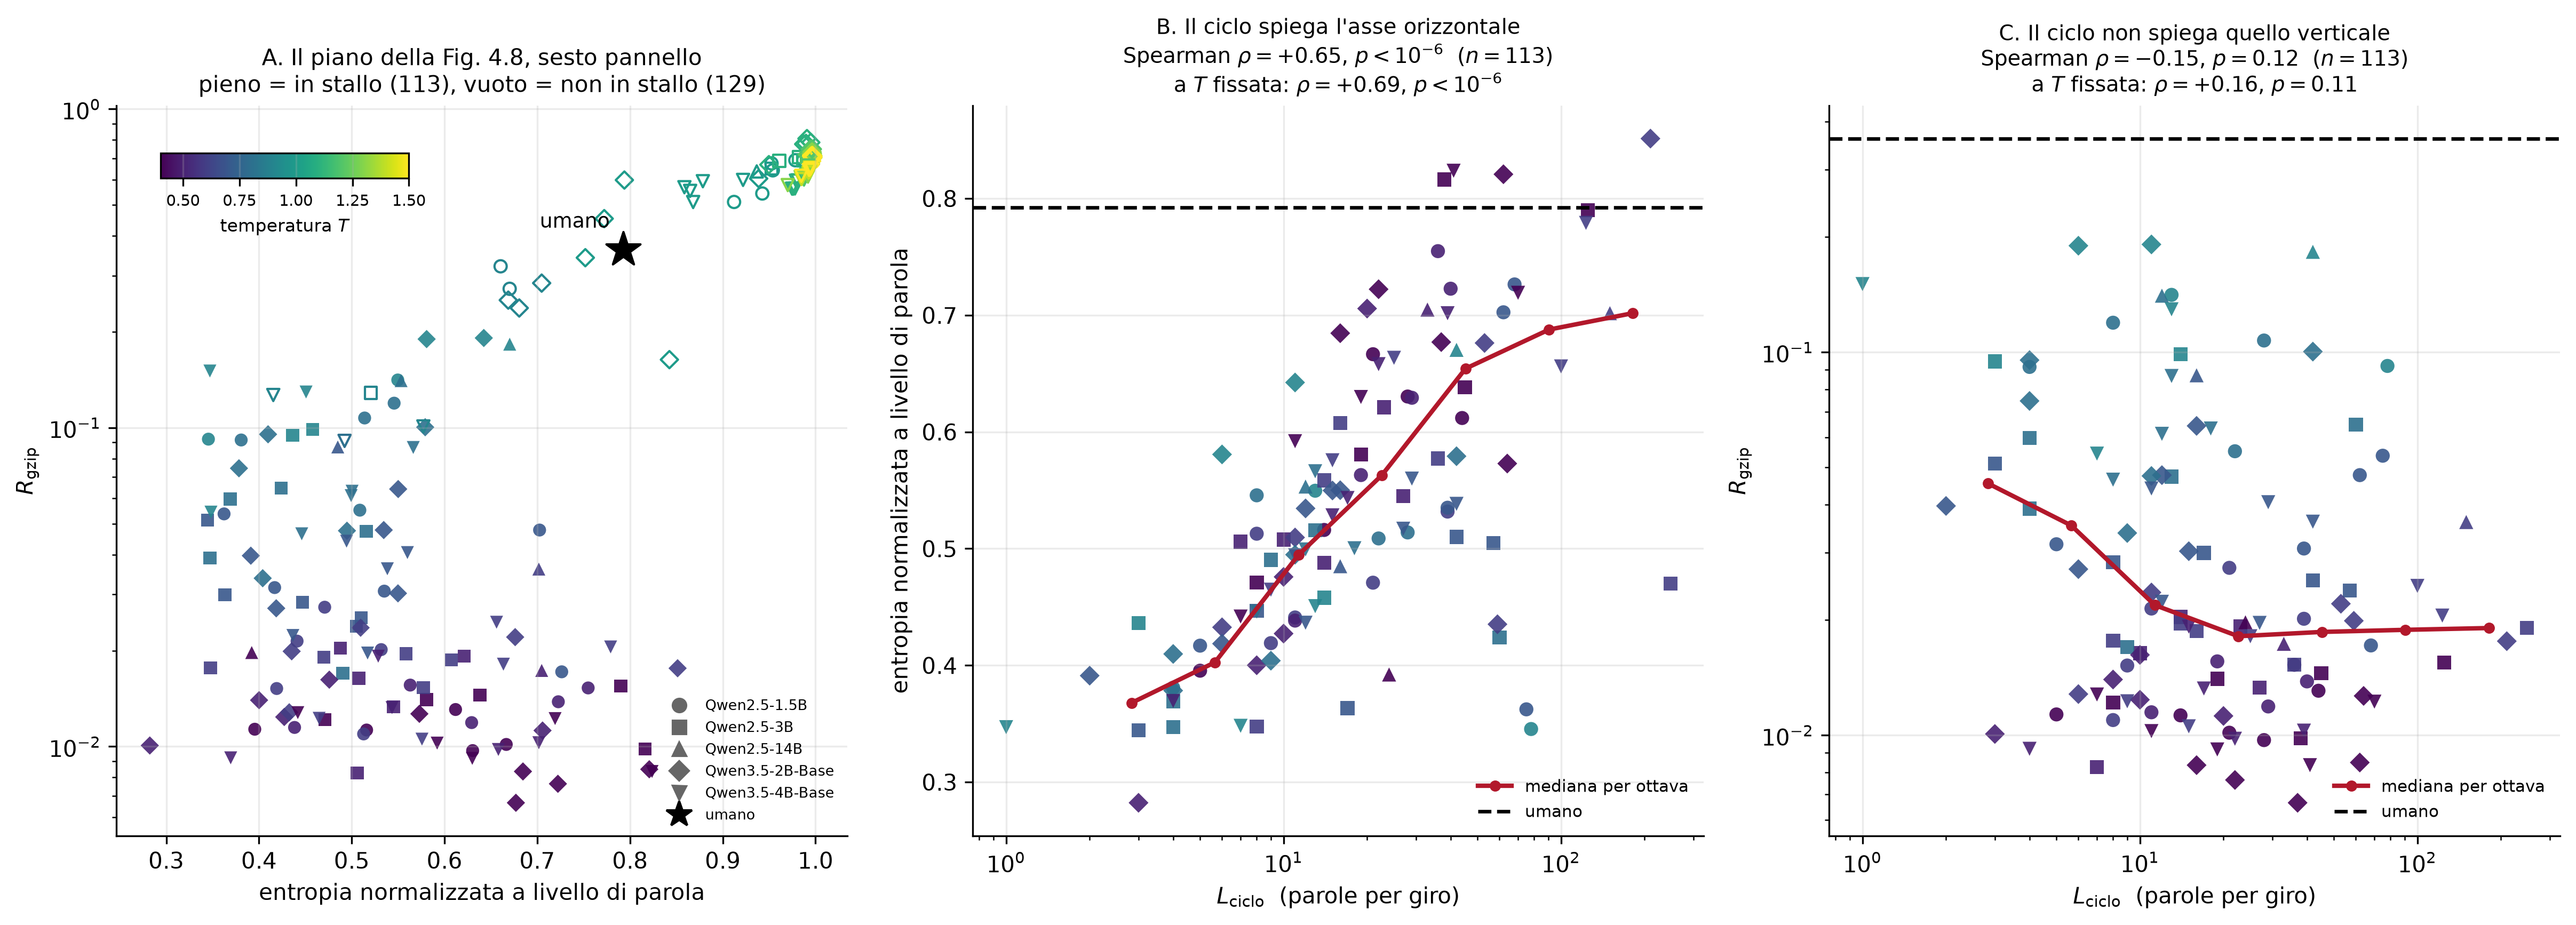
\includegraphics[width=\textwidth]{figure/cap4_ciclo_entropia.png}
  \caption{Lunghezza del ciclo ripetuto in fase di stallo. A: il piano
  entropia--comprimibilità della Figura~\ref{fig:compressione}, con i documenti
  in stallo a simbolo pieno e gli altri a simbolo vuoto; il colore codifica la
  temperatura e la forma il modello. B: entropia di parola contro lunghezza del
  ciclo, con la mediana per ottava. C: rapporto di compressione contro la stessa
  grandezza. La lunghezza del ciclo ordina l'asse orizzontale del piano e non
  quello verticale.}
  \label{fig:ciclo}
\end{figure}


% ---------------------------------------------------------------------
\section{Le tre fasi}
\label{sec:fasi-risultati}

Le misure precedenti descrivono il testo generato senza classificarlo. La regola
del §\ref{sec:tre-fasi} permette invece di assegnare ciascun documento a una
fase, e questa sezione ne riporta l'esito.

La traiettoria della~\eqref{eq:traiettoria} è costruita sui vettori GloVe a 100
dimensioni già impiegati nel §\ref{sec:token}, e l'autocorrelazione è calcolata
sui primi cento lag, misurati in parole. Il fit del GAPELMAPER usa invece un
intervallo più ampio, fino a 600 parole, perché distinguere una legge di potenza
da un esponenziale richiede più di una decade di distanze. Il livello di rumore
$\eta$ è stimato su una singola permutazione della traiettoria di ciascun
documento, con seme fissato.

Le due soglie della regola valgono $\kappa_{\min} = 0.50$ e $\Phi_{\min} = 3$.
La prima è deliberatamente permissiva: serve a escludere i documenti in cui meno
di metà delle parole ha un vettore, cioè quelli in cui la traiettoria è fatta per
lo più di zeri, e non a selezionare i documenti buoni. La seconda separa i due
gruppi in cui $\Phi$ effettivamente si distribuisce, e la sua posizione è poco
critica: come mostra la Figura~\ref{fig:transizioni}, fra la fase periodica e
quella successiva $\Phi$ cambia di due ordini di grandezza, cosicché qualunque
soglia compresa fra $1$ e $5$ produce la stessa classificazione. Il
§\ref{sec:tstar} riprende il punto trattando la fine della fase periodica come
uno degli otto criteri di temperatura critica.

La Figura~\ref{fig:acf} mostra come questa autocorrelazione cambia lungo lo
sweep. Fino a $T = 0.9$ la curva oscilla con periodo definito e ampiezza
prossima all'unità: il testo ripete un ciclo di parole, e a distanza pari a un
multiplo del ciclo ogni vettore ritrova sé stesso. Il periodo si accorcia al
crescere della temperatura, da dieci parole a $T = 0.5$ a circa tre a $T =
0.8$, mentre l'ampiezza scende da $0.98$ a $0.72$. Fra $T = 0.9$ e $T = 1.0$
la struttura periodica scompare del tutto: l'ampiezza cade a $0.036$ e la
curva diventa un decadimento monotono, senza più oscillazione. A $T = 1.3$
l'intera curva è contenuta nella banda di rumore stimata mescolando le parole
del documento, cioè non è distinguibile dal caso.

Il confronto con il testo umano chiarisce quanto entrambi i regimi siano
lontani dal linguaggio naturale. L'autocorrelazione del romanzo non è
periodica, con $\max\lvert\mathrm{FFT}\rvert$ pari a $1.16$, ben sotto la
soglia $3$, ma è nettamente sopra il livello di rumore su tutti i cento lag
esaminati, e il suo spettro decade in modo regolare invece di essere piatto.
Nessuna delle temperature campionate riproduce questa combinazione: sotto la
transizione la correlazione è troppo forte e periodica, sopra è assente.

\begin{figure}[htbp]
  \centering
  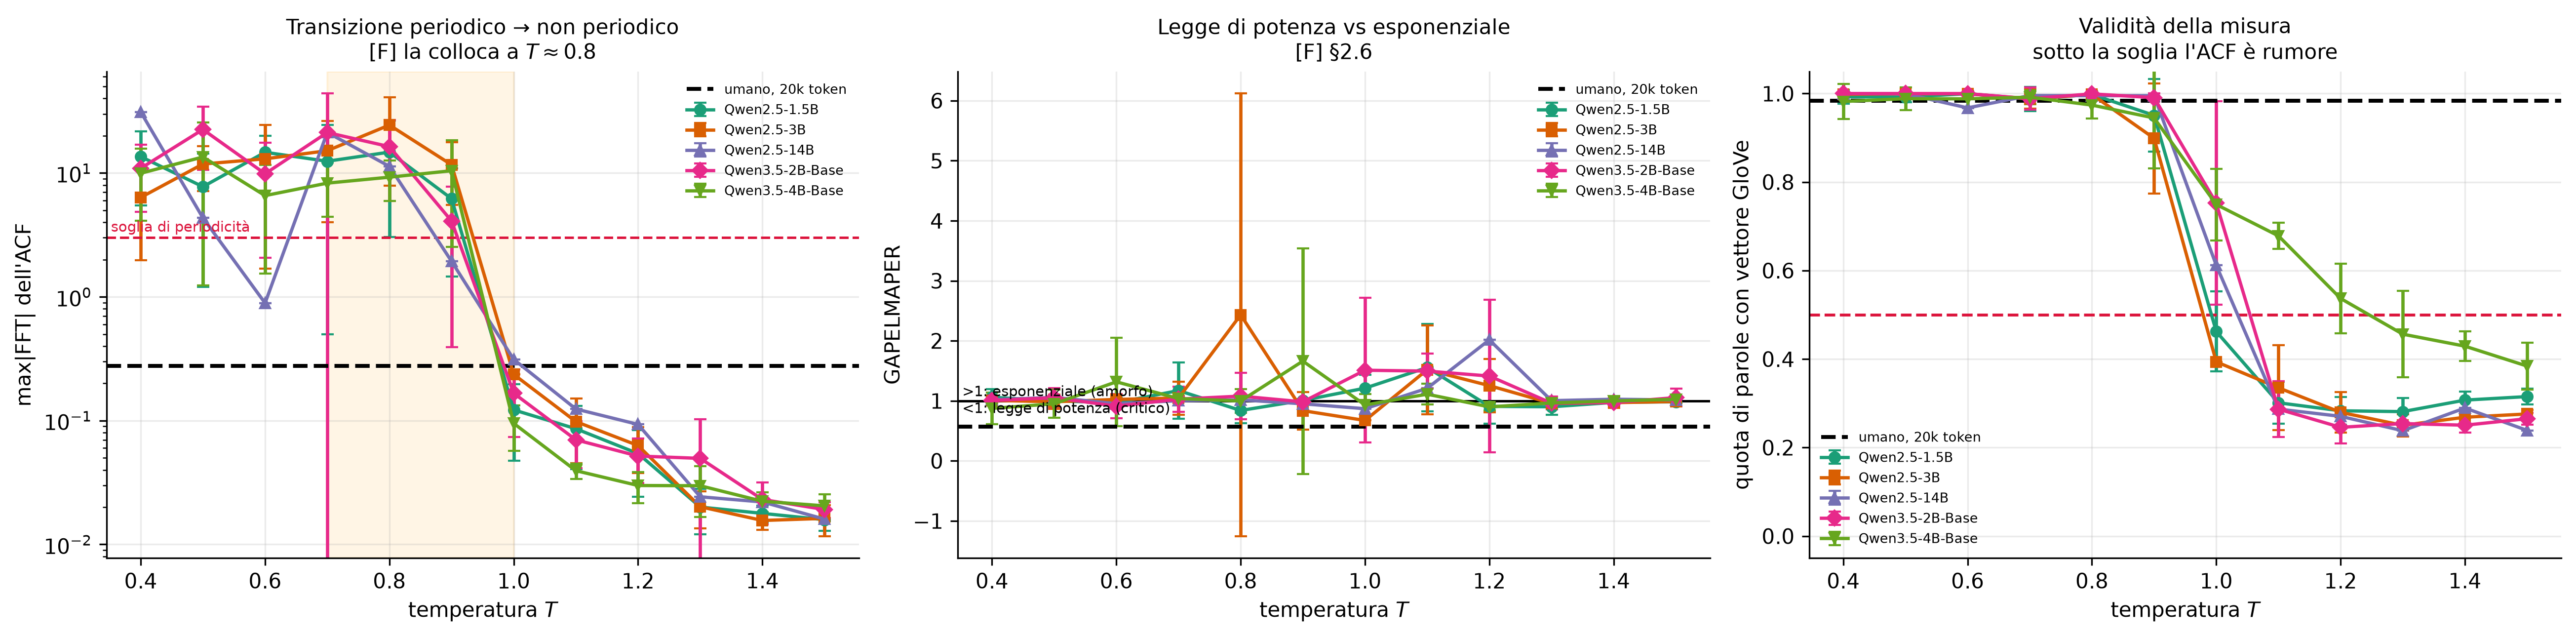
\includegraphics[width=\textwidth]{figure/cap4_transizioni_fase.png}
  \caption{Parametro di periodicità, GAPELMAPER e copertura degli embedding in
  funzione della temperatura. Il primo pannello è in scala logaritmica. Il terzo
  riporta la quota di parole dotate di un vettore, che è la condizione di
  validità delle altre due misure.}
  \label{fig:transizioni}
\end{figure}

\begin{figure}[htbp]
  \centering
  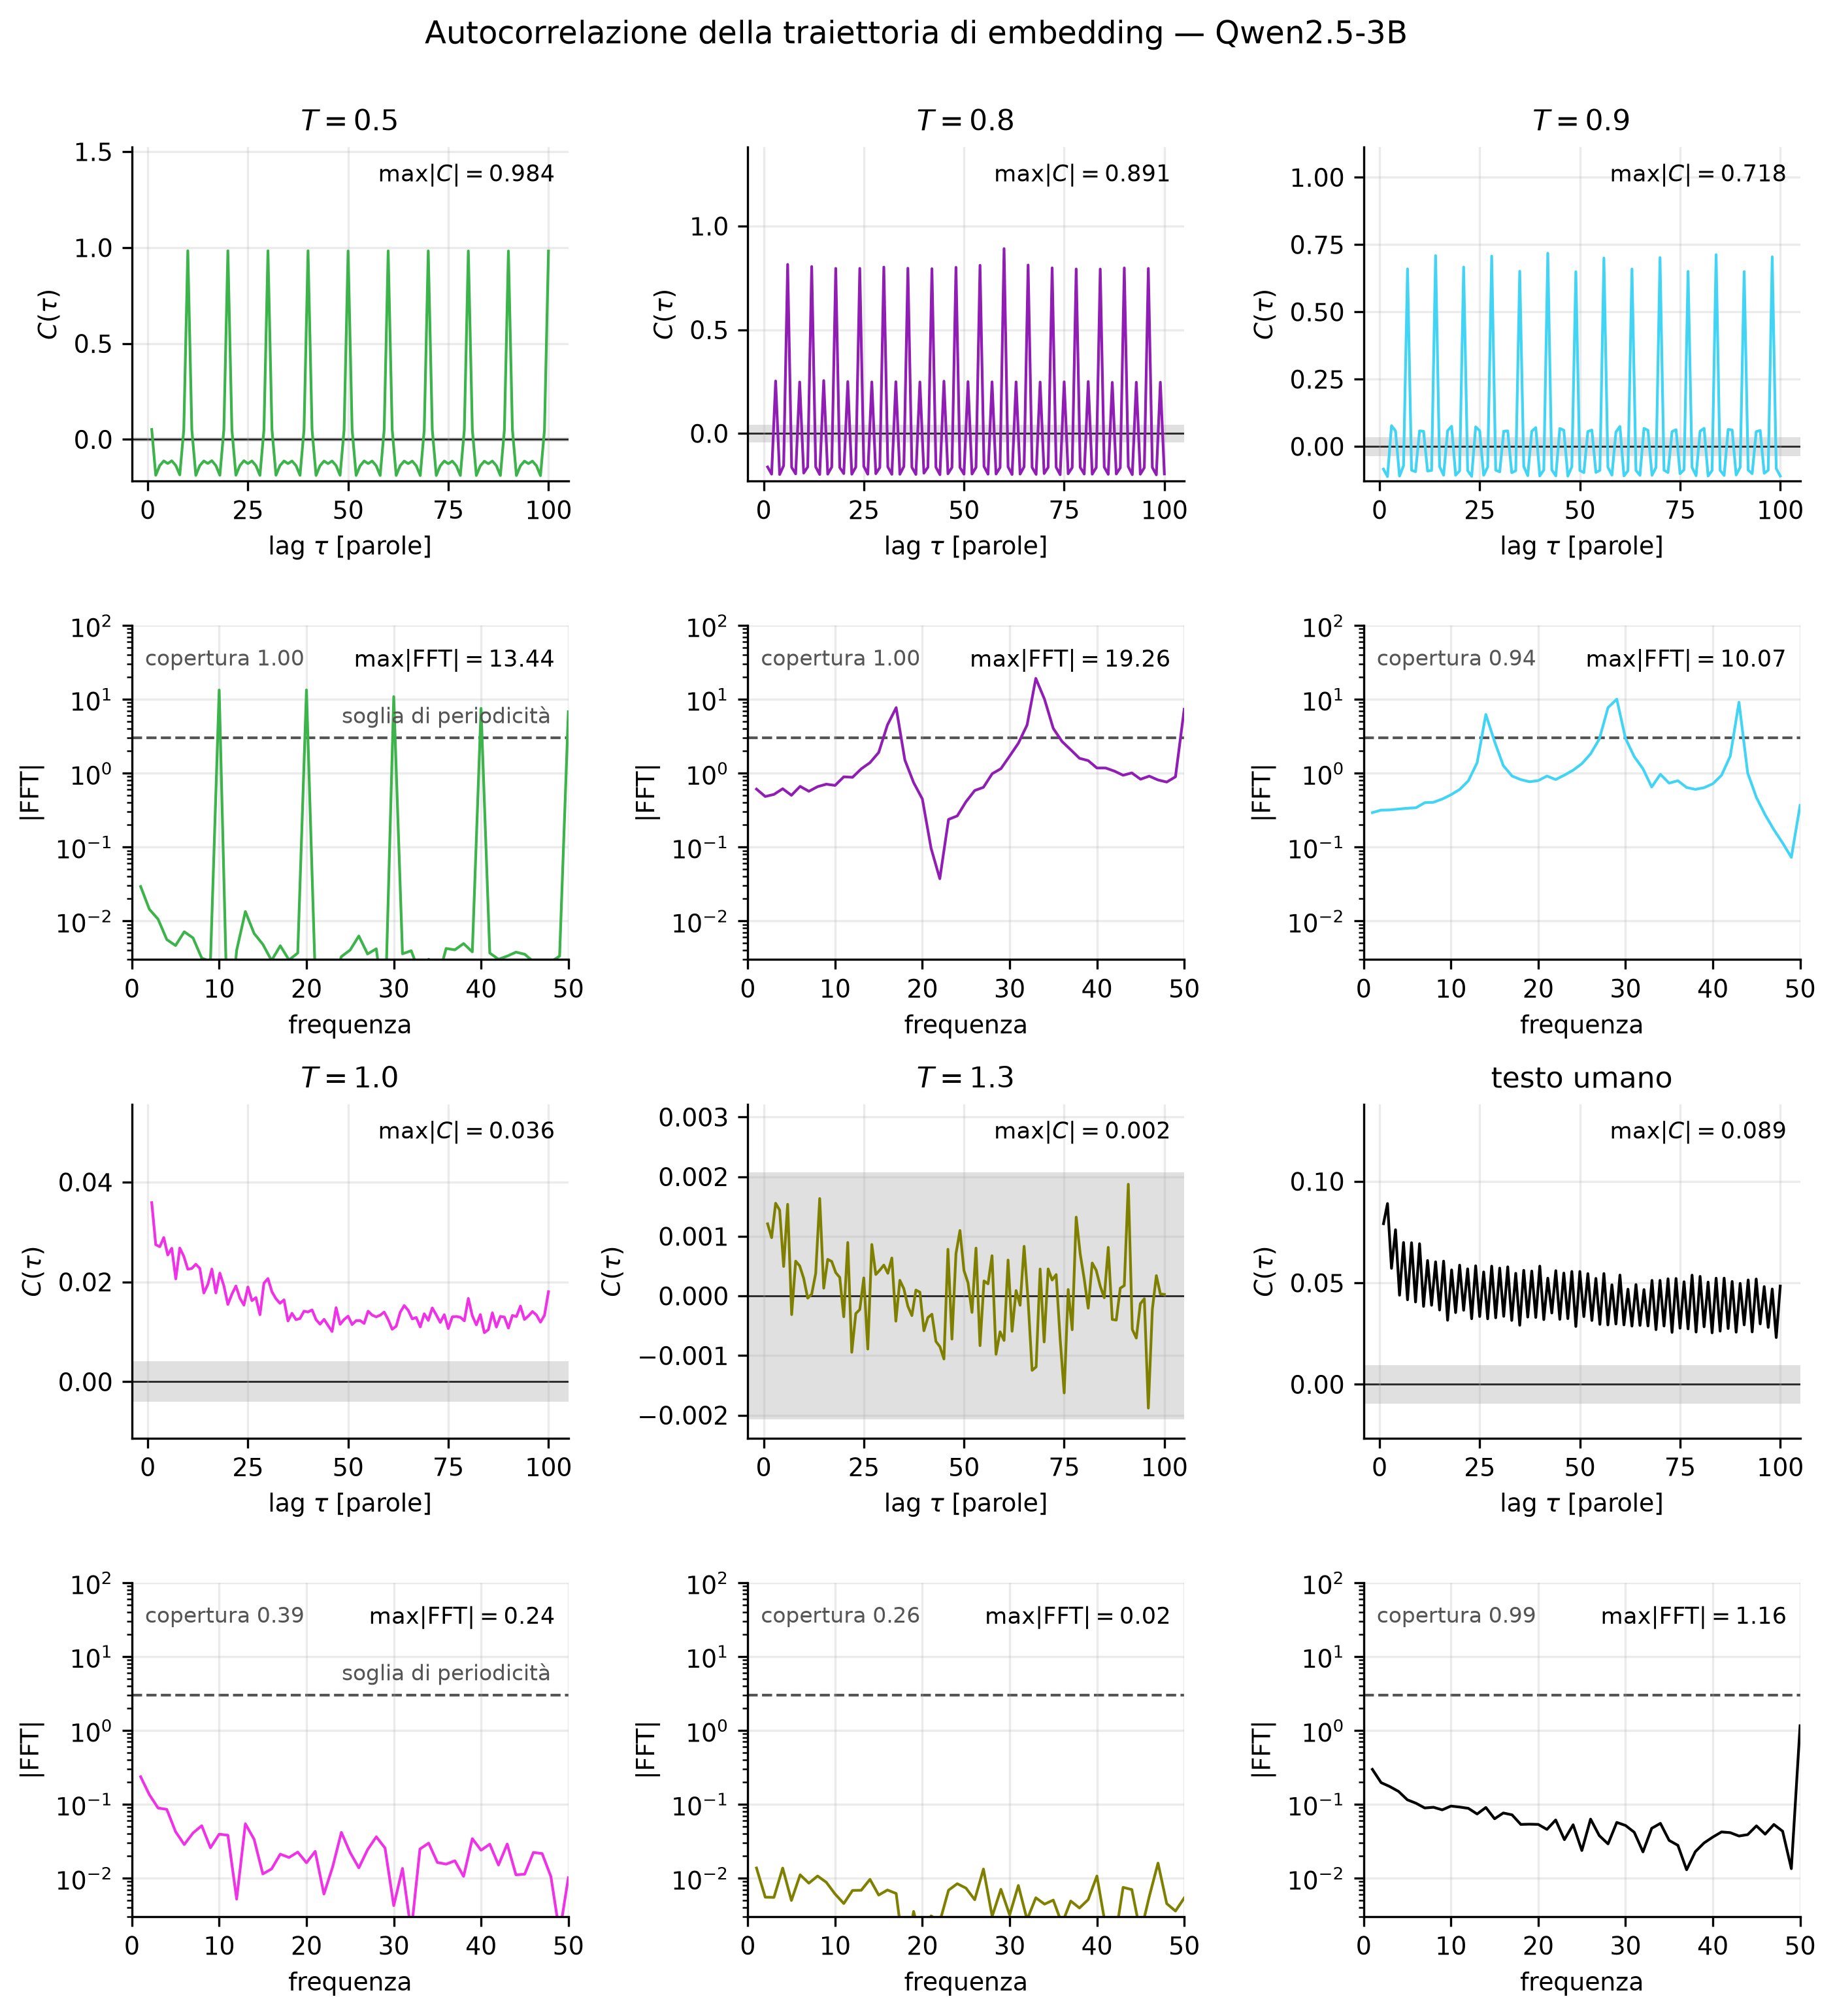
\includegraphics[width=\textwidth]{figure/cap4_acf_Qwen25_3B.png}
  \caption{Autocorrelazione della traiettoria di embedding per il modello
  Qwen2.5-3B a cinque temperature e sul testo umano di riferimento. In ciascuna
  coppia di riquadri il primo riporta $C(\tau)$ per lag da 1 a 100 parole e il
  secondo il modulo della sua trasformata di Fourier. La banda grigia è il
  livello di rumore, stimato ricalcolando $C(\tau)$ dopo aver permutato a caso
  le parole dello stesso documento; la linea tratteggiata è la soglia
  $\max\lvert\mathrm{FFT}\rvert = 3$ che separa la fase periodica. Per ogni
  temperatura è mostrato il campione di periodicità mediana, non il più marcato.
  La scala verticale di $C(\tau)$ è propria di ciascun riquadro, perché
  l'ampiezza varia di oltre due ordini di grandezza fra le temperature basse e
  quelle alte; il valore di picco è riportato dentro il riquadro. La scala dello
  spettro è invece logaritmica e comune, così i sei casi si confrontano
  direttamente.}
  \label{fig:acf}
\end{figure}

Il parametro d'ordine della prima transizione è il massimo modulo della
trasformata oltre il primo coefficiente, e il suo crollo è il risultato più
netto dell'intero capitolo. La media su tutti i modelli vale $16.0$ a
$T = 0.8$, scende a $7.5$ a $T = 0.9$ e precipita a $0.145$ a $T = 1.0$: un
fattore cinquanta in un solo passo di temperatura, e cento rispetto al massimo
di $T = 0.8$. Prosegue poi fino a $0.018$ a
$T = 1.5$, complessivamente tre ordini di grandezza sotto il massimo. Le cinque
curve dei diversi modelli si sovrappongono quasi esattamente, come mostra la
Figura~\ref{fig:transizioni}.

Anche questa soglia va confrontata con la fonte.
In~\cite{mikhaylovskiy2025states} la transizione dalla fase periodica è
collocata attorno a $t = 0.8$, con il testo dichiarato già non periodico a
$t = 1$, mentre qui la periodicità sopravvive fino a $T = 0.9$ e scompare a
$T = 1.0$. Lo spostamento verso l'alto è coerente con l'effetto del prompt
descritto nel §\ref{sec:protocollo}, che ritarda la comparsa delle proprietà
del regime disordinato.

\paragraph{Il secondo criterio non discrimina.} La distinzione fra stato
critico e fase amorfa dovrebbe essere operata dal GAPELMAPER, ma sui dati di
questo lavoro tale criterio non funziona. Il suo valore medio è $1.101$ con
deviazione standard $0.677$, e la quota di documenti con valore inferiore a 1,
cioè classificati come critici, è $0.51$: una moneta. Le barre d'errore nel
pannello centrale della Figura~\ref{fig:transizioni} sono di ampiezza
confrontabile con l'intero intervallo di variazione.

La difficoltà non è propria di questi dati. Lo stesso
\cite{mikhaylovskiy2025states} riporta che sui testi Qwen il GAPELMAPER è
raramente inferiore a 1, e che a diverse temperature del suo sweep non è
calcolabile affatto perché l'autocorrelazione assume valori negativi. Il
criterio, insomma, discrimina male anche nel lavoro che lo introduce.

Il motivo emerge dal terzo pannello. La copertura degli embedding resta sopra il
$95\%$ fino a $T = 0.9$, ma crolla a $0.64$ a $T = 1.0$ e a circa $0.31$ oltre
$T = 1.2$: nel regime in cui il GAPELMAPER dovrebbe distinguere le ultime due
fasi, l'autocorrelazione è calcolata su una minoranza delle parole e non
contiene più segnale. Per questa ragione i documenti che non superano la soglia
di copertura sono marcati come non valutabili anziché classificati, come
anticipato nel §\ref{sec:tre-fasi}. Senza tale precauzione il criterio avrebbe
assegnato una fase a documenti in cui non c'è nulla da misurare.

\paragraph{Il diagramma di fase.}
La Figura~\ref{fig:diagramma} riporta la composizione delle fasi per modello e
temperatura. Il quadro è coerente su tutti e cinque: fase periodica fino a
$T = 0.9$, dove la classificazione è ancora periodica per 13 documenti su 18;
scomparsa completa della periodicità a $T = 1.0$; documenti prevalentemente non
valutabili da $T = 1.1$ in poi, e completamente tali a $T \ge 1.4$.

\begin{figure}[htbp]
  \centering
  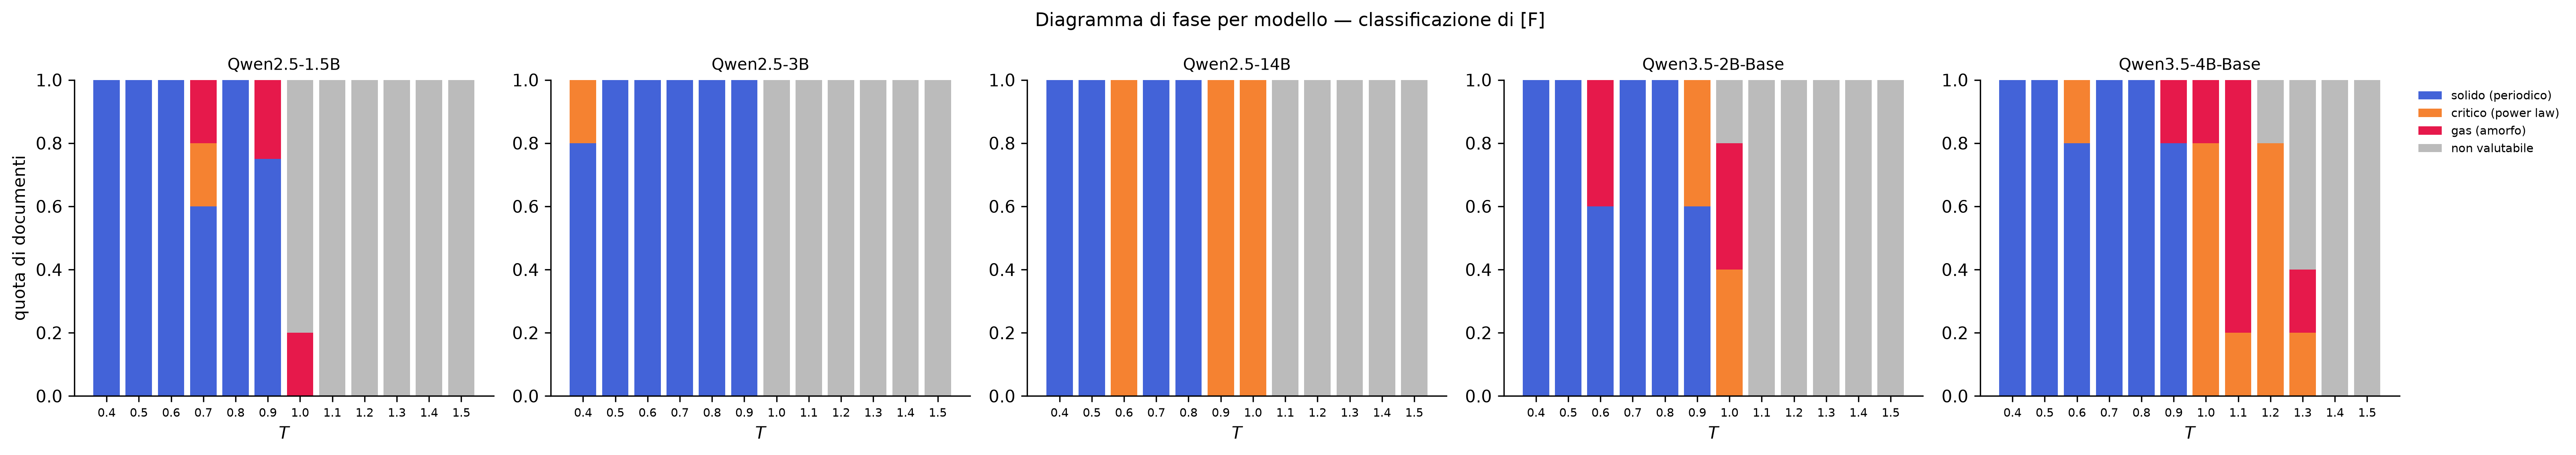
\includegraphics[width=\textwidth]{figure/cap4_diagramma_fase.png}
  \caption{Composizione delle fasi per modello e temperatura. La categoria «non
  valutabile» raccoglie i documenti che non superano la soglia di copertura
  degli embedding.}
  \label{fig:diagramma}
\end{figure}

Le tre modalità di fallimento del §\ref{sec:fallimenti} trovano qui la loro
interpretazione. La degenerazione per ripetizione è la fase periodica; la
degenerazione dell'alfabeto e del lessico corrisponde alla regione in cui la
misura non è più applicabile, che è a sua volta il segnale della fase amorfa. Il
testo non degenerato esiste solo nella striscia sottile fra le due, ed è la
stessa striscia in cui tutte le misure delle sezioni precedenti si avvicinano ai
valori umani.

% ---------------------------------------------------------------------
\section{Convergenza della temperatura critica}
\label{sec:tstar}

Le sezioni precedenti individuano ciascuna una temperatura privilegiata. Poiché
i criteri provengono da lavori indipendenti e misurano proprietà diverse del
testo, il loro accordo o disaccordo è esso stesso un risultato.

La Tabella~\ref{tab:tstar} riporta la temperatura selezionata da ciascun
criterio per ciascun modello. Due criteri sono intrinseci, nel senso che
individuano un estremo della curva senza far riferimento al testo umano: il
minimo del MAPE e la fine della fase periodica. Gli altri sei selezionano la
temperatura alla quale la misura si avvicina di più alla baseline umana.

\begin{table}[htbp]
\centering
\small
\begin{tabular}{@{}lccccc@{}}
\toprule
Criterio & 1.5B & 3B & 14B & 3.5-2B & 3.5-4B \\
\midrule
MAPE minimo                                  & 0.9 & 0.9 & 0.7 & 0.9 & 0.9 \\
$D_s$ minima dal testo umano                 & 0.9 & 0.9 & 0.9 & 0.9 & 1.0 \\
Fine della fase periodica                    & 1.0 & 1.0 & 0.6 & 1.0 & 1.0 \\
$R_{\mathrm{gzip}}$ più vicino all'umano     & 0.9 & 1.0 & 0.9 & 1.0 & 1.0 \\
$\alpha$ più vicino all'umano                & 1.0 & 1.5 & 1.3 & 1.0 & 1.0 \\
$R$ più vicino all'umano                     & 1.0 & 1.1 & 1.1 & 1.1 & 1.0 \\
$\gamma_H$ più vicino all'umano              & 1.1 & 1.0 & 1.3 & 1.1 & 1.3 \\
$\alpha_{\mathrm{DFA}}$ più vicino all'umano & 1.2 & 1.1 & 1.1 & 1.1 & 1.1 \\
\midrule
\textbf{mediana}                             & \textbf{1.0} & \textbf{1.0} &
\textbf{1.0} & \textbf{1.0} & \textbf{1.0} \\
\bottomrule
\end{tabular}
\caption{Temperatura selezionata da ciascun criterio, per ciascun modello. La
mediana vale $1.0$ per tutti e cinque i modelli, benché i singoli criteri
spazino da $0.6$ a $1.5$.}
\label{tab:tstar}
\end{table}

Il risultato principale del capitolo è la riga in fondo alla tabella. Otto
criteri tratti da quattro lavori indipendenti, costruiti per scopi diversi e mai
progettati per concordare, danno una mediana identica per tutti e cinque i
modelli. La convergenza non era scontata: i criteri misurano la distribuzione
delle frequenze, la crescita del vocabolario, le correlazioni a lungo raggio, la
comprimibilità e la periodicità dell'autocorrelazione, cioè proprietà che nulla
obbliga a coincidere.

\begin{figure}[htbp]
  \centering
  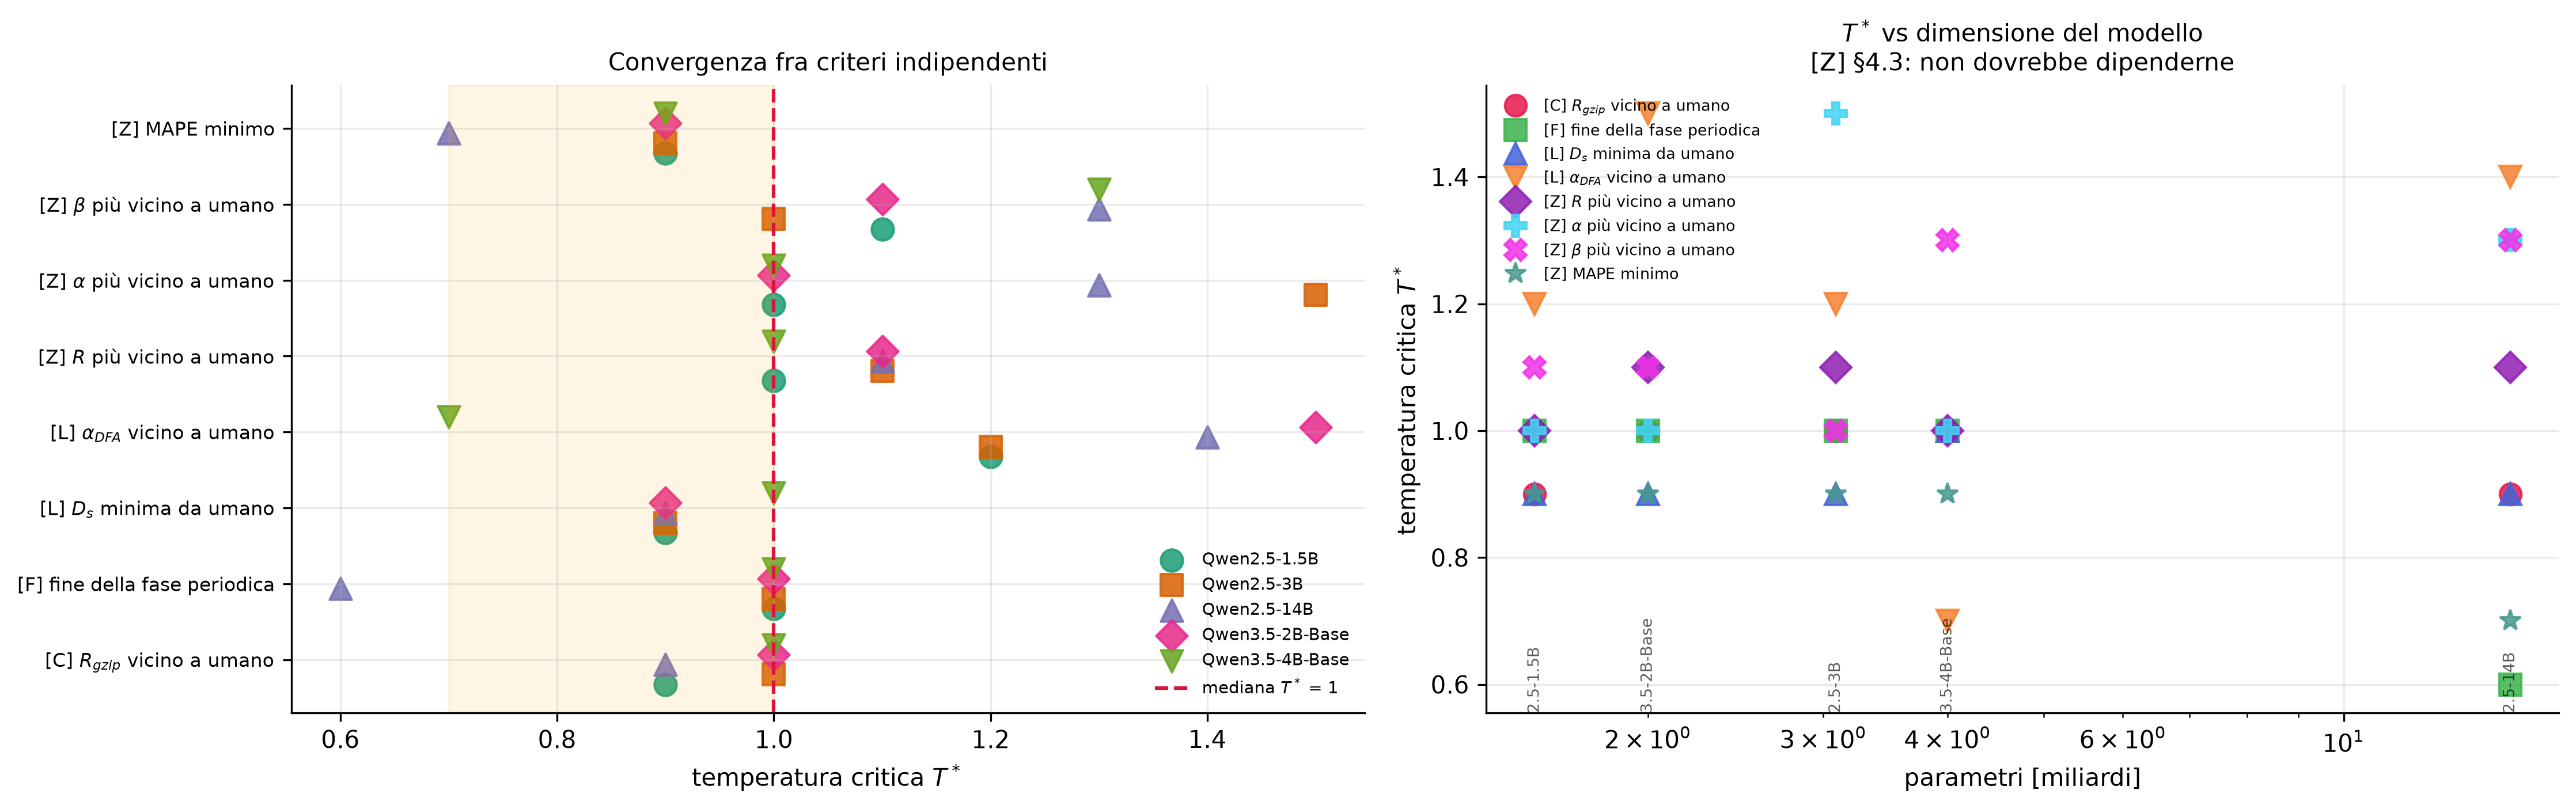
\includegraphics[width=\textwidth]{figure/cap4_temperatura_critica.png}
  \caption{A sinistra, la temperatura selezionata da ciascun criterio; la linea
  tratteggiata è la mediana complessiva e la banda la regione fra $0.7$ e $1.0$.
  A destra, la stessa quantità in funzione del numero di parametri del modello.}
  \label{fig:tstar}
\end{figure}

\paragraph{Dipendenza dalla dimensione del modello.}
La Figura~\ref{fig:tstar} riporta a destra la temperatura critica in funzione
del numero di parametri. La correlazione di rango è $\rho = -0.01$ con
$p = 0.93$ su quaranta osservazioni: nessuna dipendenza rilevabile. Il dato è
coerente con quanto riportato in~\cite{mikhaylovskiy2025zipf}, dove la posizione
dell'ottimo risulta indipendente dalla dimensione per tutte le famiglie
esaminate.

Un'assenza di correlazione misurata su cinque modelli appartenenti a due
famiglie non dimostra l'indipendenza: dimostra che, entro l'intervallo di
dimensioni esplorato e con la potenza statistica disponibile, non emerge
alcuna dipendenza. È coerenza con la letteratura, non conferma indipendente.

\paragraph{Una discordanza fra criteri.}
Due criteri si collocano sistematicamente fuori dal gruppo, e la loro distanza
dagli altri è essa stessa un risultato: mediarli insieme al resto la
cancellerebbe.

Il minimo del MAPE cade a $0.9$, mentre la fine della fase periodica cade a
$1.0$: alla temperatura in cui la distribuzione delle frequenze è più vicina a
una legge di potenza, l'autocorrelazione è ancora periodica per la maggioranza
dei documenti. Le due misure non si contraddicono, perché guardano oggetti
diversi, la statistica dei conteggi l'una e la struttura sequenziale l'altra,
e la loro distanza quantifica il fatto che le due proprietà non compaiono
simultaneamente. Il testo acquista una distribuzione di frequenze verosimile
prima di perdere la ripetizione.

Il criterio basato su $\alpha_{\mathrm{DFA}}$ merita una nota, perché il suo
esito dipende dall'ordine del detrending. Con il grado 1 seleziona temperature
fra $0.7$ e $1.5$, il più disperso dei nove; con il grado 2, che è quello
adottato qui per la ragione data nel §\ref{sec:robustezza}, si allinea agli
altri e sceglie $1.1$ per quattro modelli su cinque. La mediana per modello vale
$1.0$ in entrambi i casi. Resta valida l'avvertenza del
§\ref{sec:dfa-risultati}: alle basse temperature quell'esponente è instabile
fra documenti, e viene riportato per completezza anziché usato come criterio a
sé stante.

Una divergenza analoga fra criteri è documentata
in~\cite{mikhaylovskiy2025zipf} per i modelli Llama di grandi dimensioni, dove
le leggi di Zipf e di Heaps individuano temperature critiche sensibilmente
diverse. Il fenomeno non sembra dunque un artefatto di questo lavoro.

% ---------------------------------------------------------------------
\section{Che cosa lo sweep ha stabilito}
\label{sec:sintesi-cap4}

Tre risultati emergono dalle sezioni precedenti, di natura diversa fra loro.

Il primo è l'esistenza di una temperatura privilegiata, e la sua posizione. Otto
criteri costruiti per scopi diversi e tratti da quattro lavori indipendenti
danno una mediana identica, $T = 1.0$, per tutti e cinque i modelli, senza
dipendenza rilevabile dalla dimensione. Il secondo è che l'ottimo è stretto: la
transizione si consuma quasi interamente fra $T = 0.9$ e $T = 1.0$, dove il
parametro di periodicità cade di un fattore cinquanta, l'entropia passa da
$0.332$ a $5.77$ bit per carattere e il rapporto di compressione da $0.107$ a
$0.650$. Uno sweep a passo $0.1$ è appena sufficiente a risolvere quella
finestra.

Il terzo è l'esito negativo su cui poggia il capitolo successivo. L'esistenza
dell'ottimo è un fatto generale, ma la sua \emph{qualità} non lo è: due modelli
su cinque portano il MAPE al livello del testo umano e gli altri no. La
compressione condizionata non raggiunge il valore umano a nessuna temperatura,
ma per una ragione che non riguarda la struttura semantica: sotto la transizione
il testo ripete un ciclo e la seconda metà è prevedibile per costruzione, sopra
non è più linguaggio e non è prevedibile da nulla. Soprattutto, i documenti che
superano tutte e tre le soglie di non
degenerazione sono due su \num{242}. Il corpus generato lungo lo sweep non
sostiene quindi un'analisi semantica, ed è la ragione per cui il
Capitolo~\ref{cap:risultati2} cambia dominio anziché proseguire su questo.

Il capitolo non stabilisce però tutto. La convergenza dei criteri dice dove il
testo generato somiglia di più a quello umano secondo misure che ignorano il
significato; non dice se in quel punto il testo sia organizzato attorno a un
contenuto. È la domanda posta nel §\ref{sec:intro-domanda}, e richiede gli
strumenti del §\ref{sec:burst}.

% =====================================================================
%  Capitolo 5 — Burstiness lessicale in corpora umani e generativi
%  Incluso da main.tex con % =====================================================================
%  Capitolo 5 — Burstiness lessicale in corpora umani e generativi
%  Incluso da main.tex con % =====================================================================
%  Capitolo 5 — Burstiness lessicale in corpora umani e generativi
%  Incluso da main.tex con \input{capitolo5_burstiness}
%
%  Tre lunghezze di analisi con corpora diversi, da non confondere:
%    fattibilità  50 000 caratteri, 40 voci  (§5.2)
%    analisi      60 000 caratteri, 39 terne (§5.3--5.7)
%    robustezza   80 000 caratteri, 35 terne (§5.8)
% =====================================================================

\chapter{Burstiness lessicale in corpora umani e generativi}
\label{cap:risultati2}

% ---------------------------------------------------------------------
\section{Perché un secondo corpus}
\label{sec:perche-wiki}

Questo capitolo nasce da un esito negativo del precedente. Il
§\ref{sec:fallimenti} ha mostrato che dei \num{242} documenti generati lungo lo
sweep soltanto due non ricadono in alcuna modalità di degenerazione, ed entrambi
si trovano a $T = 1.0$. Il protocollo introdotto nel §\ref{sec:burst} è però un
protocollo semantico: richiede di individuare in ciascun testo le parole che ne
portano il contenuto e di misurare come si distribuiscono le distanze fra le
loro occorrenze successive. Su un testo che ripete lo stesso ciclo di parole, o
su una sequenza degenerata nel senso opposto, 
quelle distanze si calcolano ancora ma non misurano più la
persistenza di un tema. Applicare il protocollo al corpus dello sweep
restituirebbe numeri privi di contenuto.

Il confronto viene quindi spostato su un dominio in cui la qualità del testo
non è una variabile. Wikipedia e Grokipedia trattano le stesse voci, la prima
scritta da esseri umani e la seconda generata da un modello linguistico, ed
entrambe producono prosa espositiva ben formata. Appaiare le due enciclopedie
per titolo tiene inoltre fisso l'argomento trattato: la voce
\emph{Albert Einstein} di Wikipedia e quella di Grokipedia parlano della stessa
cosa, e qualunque differenza nella statistica degli intervalli non può essere
attribuita a un argomento diverso. I corpora sono descritti nel §\ref{sec:corpora}, e le
due versioni di Grokipedia nel §\ref{sec:paternita}.

Il romanzo di riferimento resta nell'analisi come ancora letteraria: è il
dominio su cui il protocollo è stato formulato, e serve a dire quanto la prosa
enciclopedica si discosti già di per sé dal caso studiato in origine.

% ---------------------------------------------------------------------
\section{Il protocollo regge sulla prosa enciclopedica}
\label{sec:fattibilita}

Prima di confrontare due enciclopedie occorre stabilire che l'effetto da
confrontare esista nella prima. Il protocollo di Altmann è stato costruito e
validato su romanzi, e la prosa enciclopedica ha una struttura diversa: non ha
trama, procede per sezioni tematiche dichiarate da titoli, e la persistenza di
un argomento vi si manifesta in modo più rigido. Che le parole di contenuto vi
risultino più \emph{bursty} dei propri controlli non è quindi scontato.

La verifica è stata condotta su \num{40} voci di Wikipedia troncate a
\num{50000} caratteri, contro \num{20} segmenti del romanzo della stessa
lunghezza: è la fase di fattibilità della Tabella~\ref{tab:fasi}, l'unica del
capitolo a impiegare quella lunghezza e quel numero di voci, e i suoi
denominatori non vanno confusi con quelli delle sezioni successive. La
Figura~\ref{fig:wiki-fattibilita} ne riporta l'esito. Il primo
pannello confronta ciascuna parola chiave con il proprio controllo appaiato in
frequenza e riporta la quota di confronti vinti dalla parola chiave: il valore
$0.5$ corrisponde all'assenza di effetto. Su Wikipedia la quota vale
$197/280 = 0.704$ per il coefficiente di variazione e $216/280 = 0.771$ per
l'esponente di correlazione, con estremi inferiori degli intervalli di
confidenza pari a $0.65$ e $0.72$: l'effetto esiste. Sul romanzo le stesse
quote valgono $104/140 = 0.743$ e $123/140 = 0.879$, cioè sono più alte, ma la
differenza non annulla il segnale enciclopedico.

Il secondo pannello mostra da dove viene quel segnale, ed è utile precisare
come i suoi valori siano costruiti, perché la stessa procedura vale per tutte
le figure per livello del capitolo. Dentro ciascun testo si selezionano più
sequenze per livello: diciannove lettere, sei parole funzione, sette parole
chiave e i sette controlli appaiati. Per ognuna si misura
$\sigma_\tau/\langle\tau\rangle$ sui suoi intervalli. I valori delle sequenze
dello stesso livello si mediano poi dentro il testo, ottenendo un
numero per coppia (testo, livello); infine si media su tutti i testi del
corpus, ed è questo secondo valore a comparire nel pannello, con la barra
d'errore data dalla deviazione standard fra testi. Con questa costruzione il
coefficiente di variazione $CV$ cresce salendo lungo i quattro livelli in entrambi
i corpora e con lo stesso andamento: le lettere stanno sotto l'unità, cioè si
distribuiscono in modo più regolare di un processo di Poisson, mentre le
parole chiave arrivano a $1.51$ su Wikipedia e a $1.62$ sul romanzo. Il terzo
pannello riporta la distribuzione dei singoli testi attorno a quelle medie e
mostra che la sovrapposizione fra i due corpora è ampia, con mediane vicine e
code che si intersecano.

Il rapporto fra le due burstiness delle parole chiave vale $0.93$: la prosa
enciclopedica è meno \emph{bursty} del romanzo, ma dello stesso ordine. Il protocollo
regge, e il confronto con Grokipedia ha un segnale da rilevare.

\begin{figure}[htbp]
  \centering
  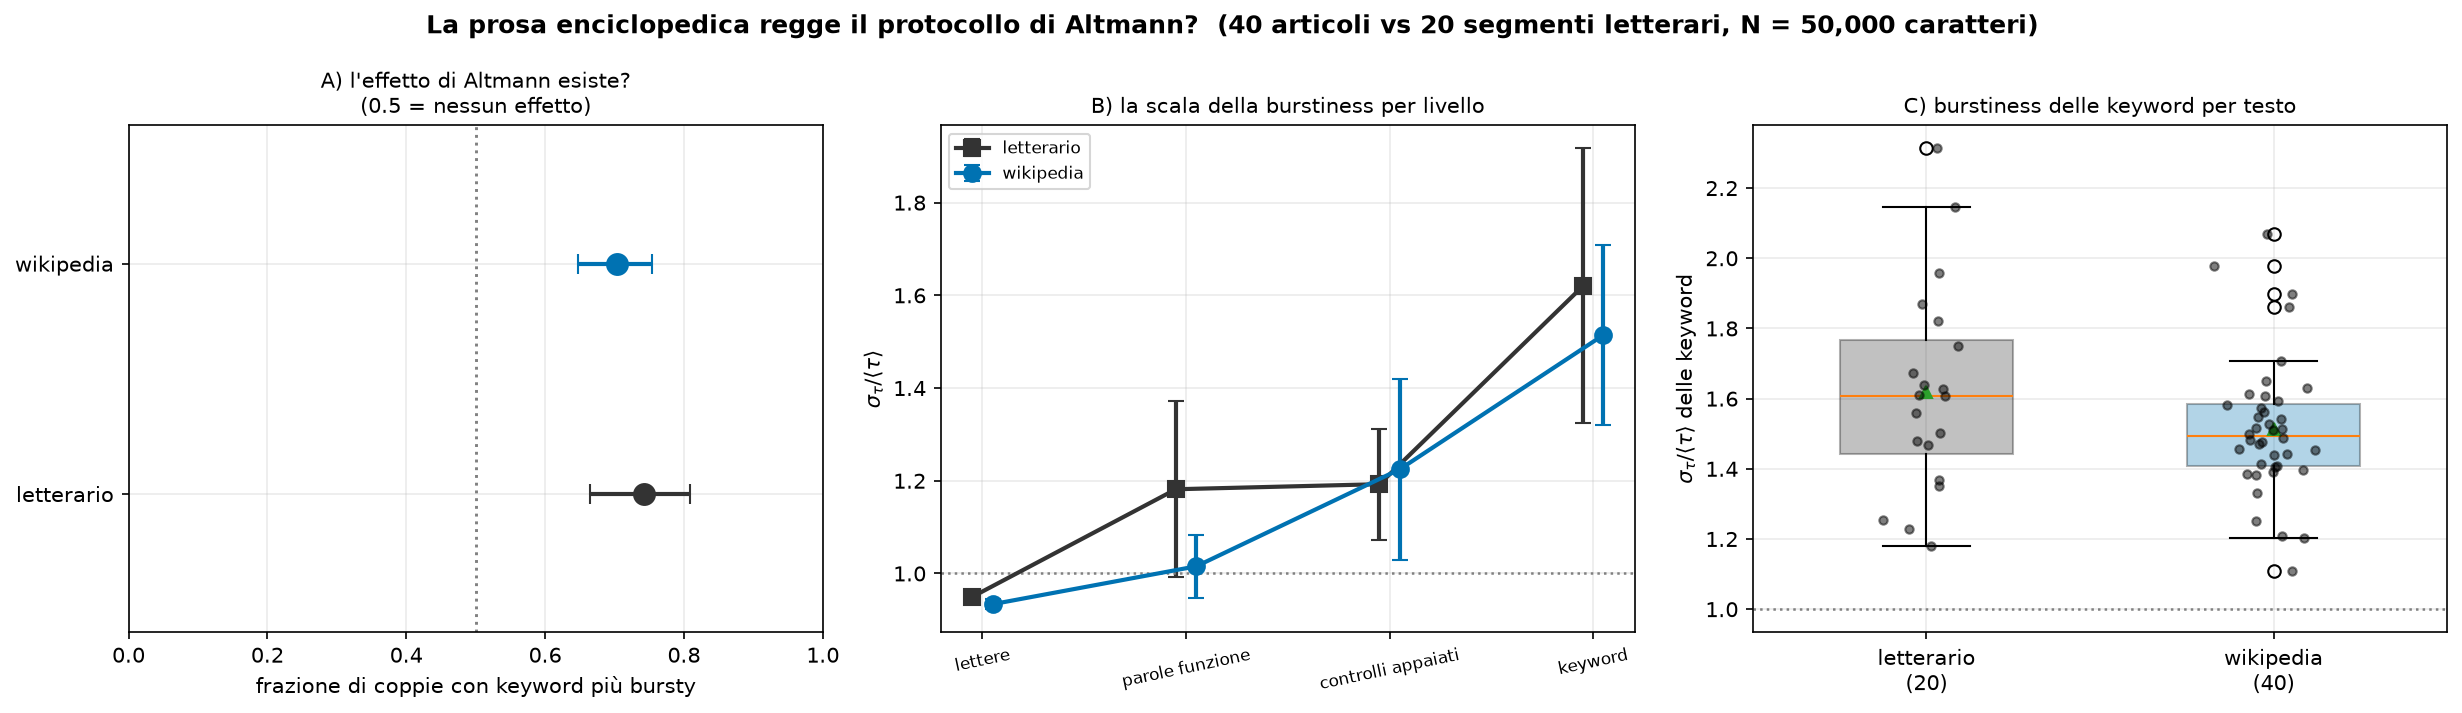
\includegraphics[width=\textwidth]{figure/cap5_wiki_altmann.png}
  \caption{Test di fattibilità del protocollo su prosa enciclopedica, condotto
  su \num{40} voci di Wikipedia e \num{20} segmenti letterari a \num{50000}
  caratteri. A: quota di confronti in cui la parola chiave supera il proprio
  controllo appaiato in frequenza, con intervallo di confidenza al $95\%$; la
  linea punteggiata a $0.5$ è l'assenza di effetto. B: coefficiente di
  variazione degli intervalli ai quattro livelli linguistici. C: distribuzione
  della burstiness delle parole chiave testo per testo. Questa è l'unica figura
  del capitolo costruita su \num{40} voci e \num{50000} caratteri; tutte le
  successive usano \num{39} terne e \num{60000} caratteri.}
  \label{fig:wiki-fattibilita}
\end{figure}

% ---------------------------------------------------------------------
\section{L'effetto nei tre corpora}
\label{sec:tre-corpora}

L'analisi principale confronta Wikipedia, le due versioni di Grokipedia e
l'ancora letteraria su \num{39} terne complete, troncate a \num{60000}
caratteri. La voce esclusa è \emph{Buddhism}, per la ragione riportata nel
§\ref{sec:paternita}: la sua versione v0.1 è ricopiata da Wikipedia, e in un
disegno appaiato un titolo che cade in un corpus deve cadere in tutti.

\paragraph{La finestra su cui l'esponente è stimato.}
L'esponente di correlazione $\hat\gamma$ è ottenuto interpolando
la~\eqref{eq:sigma} nell'intervallo fisso $t \in (100, 2000)$ caratteri.
\cite{altmann2012} adotta invece una regola relativa e ferma la finestra
all'uno per cento della lunghezza del testo. Le due scelte non sono ordinabili
una volta per tutte: applicata ai romanzi interi che quel lavoro analizza la
regola relativa dà un tetto dell'ordine di \num{10000} caratteri, molto più
largo di quello adottato qui; applicata alle finestre da \num{60000} caratteri
di questo capitolo dà $t < 600$, molto più stretto. L'intera catena è stata
ripetuta anche con la seconda. Il
livello medio di $\hat\gamma$ si abbassa di qualche centesimo, sulle parole
chiave da $1.23$ a $1.18$ per Wikipedia e da $1.32$ a $1.22$ per il romanzo,
ma l'ordinamento fra i corpora resta identico a tutti e quattro i livelli. Il
divario appaiato fra Grokipedia attuale e Wikipedia sulle parole chiave passa
da $-0.049$ a $-0.076$, cioè si accentua invece di ridursi, e resta
significativo in entrambi i casi. Le conclusioni di questo capitolo non
dipendono dunque dalla finestra scelta.

\paragraph{Tre modi di leggere il confronto.}
La Figura~\ref{fig:tre-corpora} riporta i tre modi in cui il confronto può
essere letto. Il primo pannello ripete il test del paragrafo precedente sui
quattro corpora: la quota di confronti vinti dalle parole chiave vale
$114/140 = 0.814$ sul romanzo, $189/273 = 0.692$ su Wikipedia,
$195/273 = 0.714$ su Grokipedia v0.1 e $202/273 = 0.740$ su Grokipedia nella
versione attuale. Ripetendo lo stesso test sull'esponente di correlazione
$\hat\gamma$ anziché sulla burstiness, la quota di confronti vinti dalle parole
chiave vale $0.907$ sul romanzo, $0.747$ su Wikipedia, $0.769$ su Grokipedia
v0.1 e $0.791$ su Grokipedia nella versione attuale.
L'effetto esiste ovunque, con tutti e quattro gli
intervalli di confidenza interamente sopra $0.5$, ed è massimo sul romanzo;
fra le due enciclopedie, però, non distingue: i valori di Grokipedia sono anzi
lievemente superiori a quelli di Wikipedia, con intervalli che si sovrappongono.
La domanda a cui questo pannello risponde è se la parola chiave superi il
proprio controllo a frequenza appaiata dentro lo stesso testo, e la
risposta è che ciò accade con la stessa frequenza nei due corpora enciclopedici.
Il deficit di Grokipedia, misurato dai pannelli successivi, non riguarda dunque
l'esistenza del meccanismo ma il livello assoluto della burstiness.

Il secondo pannello mostra il coefficiente di variazione ai quattro livelli e
rende visibile dove la differenza si concentra. Sulle lettere i quattro corpora
sono indistinguibili, tutti compresi fra $0.922$ e $0.950$, e sulle parole
funzione la separazione resta modesta, da $0.967$ a $1.192$. Il divario si apre
ai due livelli lessicali: sui controlli appaiati il romanzo raggiunge $1.262$,
Wikipedia $1.190$ e le due versioni di Grokipedia $1.044$ e $1.055$; sulle
parole chiave rispettivamente $1.789$, $1.536$, $1.387$ e $1.379$. 
Il terzo pannello riporta la stessa quantità testo per testo,
e mostra che la separazione non è l'effetto di pochi articoli anomali: le
distribuzioni di Wikipedia e di Grokipedia si sovrappongono, ma le loro mediane
differiscono di circa $0.25$ e la coda superiore di Wikipedia è più popolata.

\begin{figure}[htbp]
  \centering
  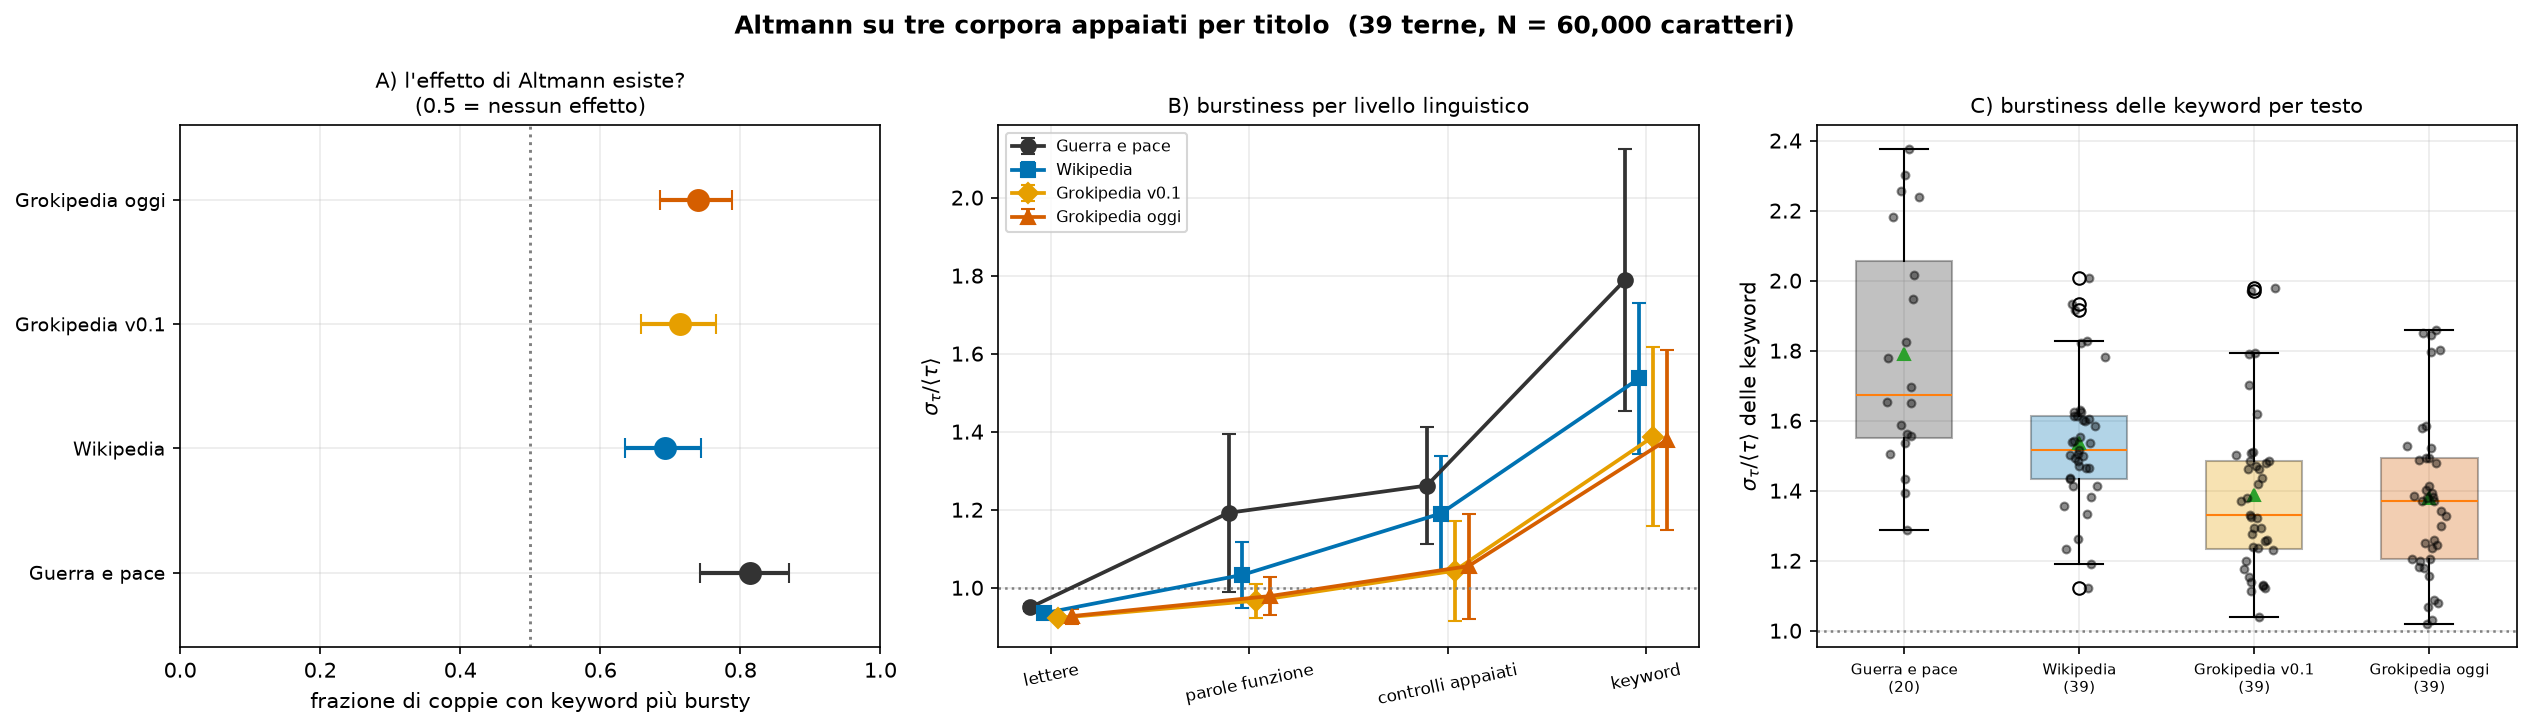
\includegraphics[width=\textwidth]{figure/cap5_tre_corpora.png}
  \caption{Il protocollo di Altmann sui quattro corpora, \num{39} terne
  appaiate per titolo a \num{60000} caratteri. A: quota di confronti vinti dalle
  parole chiave, con intervallo di confidenza al $95\%$. B: coefficiente di
  variazione degli intervalli ai quattro livelli linguistici; le barre sono
  deviazioni standard fra testi. C: burstiness delle parole chiave testo per
  testo, con mediana, quartili e singoli punti sovrapposti. Il numero di testi
  per corpus è indicato sotto ciascuna colonna.}
  \label{fig:tre-corpora}
\end{figure}

\paragraph{L'ancora letteraria è un testo, non un genere.} Il primato del
romanzo sui due livelli lessicali non sopravvive al cambio di testo. Ripetendo
l'intera misura su tre altri romanzi inglesi trattati esattamente come
\emph{Guerra e pace}, cioè \emph{Moby Dick}, \emph{Middlemarch} e \emph{David
Copperfield}, gli stessi impiegati come controllo nel
§\ref{sec:coda-risultati}, sulle parole chiave si ottiene $1.55$, $1.54$ e
$1.63$, cioè valori sostanzialmente pari a quello di Wikipedia e ben al di
sotto dell'$1.79$ di \emph{Guerra e pace}; alle parole funzione si ottiene
$1.03$, $1.08$ e $1.09$, contro l'$1.19$ del romanzo di riferimento e l'$1.03$
di Wikipedia. La distanza fra prosa letteraria e prosa enciclopedica non è
dunque un fatto generale, e l'ancora letteraria di questo capitolo va letta
per ciò che è: un termine di paragone concreto, non la misura di un genere.
Nulla di ciò che segue vi poggia, perché il risultato del capitolo è un
confronto appaiato fra le due enciclopedie, dove il romanzo non entra.

Il null model A1 restituisce un esponente medio di $0.983$ su tutte le celle,
in accordo con l'unità che deve dare per costruzione: la procedura di stima si
comporta come nel §\ref{sec:validazione} anche su questi corpora.

\paragraph{L'analogo della Figura~2 di~\cite{altmann2012}.}
La Figura~\ref{fig:altmann-fig2} riproduce sui quattro corpora la costruzione
con cui~\cite{altmann2012} presenta il proprio risultato principale, e permette
di verificarne l'aderenza riga per riga. Per ogni corpus vengono mostrate una
lettera e una parola di contenuto, ciascuna con la distribuzione cumulata degli
intervalli e con la crescita della varianza del conteggio, accanto alle stesse
curve calcolate sui due null model.

\paragraph{Quale parola mostrare.} La scelta della parola da mostrare pone un
problema che il caso della lettera non ha. Selezionare la parola chiave più
ricorrente del corpus, che è il criterio più immediato, produce oggetti
strutturalmente diversi nei due tipi di prosa: in un romanzo pesca il nome di
un personaggio, presente solo nelle scene in cui il personaggio compare,
mentre in un'enciclopedia pesca il soggetto della voce, che ricorre in quasi
ogni frase. Le due parole finirebbero alle code opposte delle rispettive
distribuzioni di burstiness, al $96$ e al $2$ percentile, e la figura
confronterebbe due casi estremi anziché due casi tipici. La parola mostrata è
quindi quella con $\sigma_\tau/\langle\tau\rangle$ più vicino alla mediana del
proprio corpus, fra quelle con almeno \num{40} occorrenze; il percentile
effettivo è riportato sopra ciascun pannello e sta fra $45$ e $57$ in tutti e
quattro i corpora. Il caso escluso ha però un interesse proprio, ed è ripreso
subito dopo la figura.

\paragraph{Che cosa mostrano le quattro righe.}
Il comportamento è allora quello descritto nel §\ref{sec:origini}, e vale su
tutte e quattro le righe. Sulla lettera la cumulata decade rapidamente e
l'esponente del null model A2 si dispone attorno all'unità, $0.94$ sul romanzo,
$0.90$ su Wikipedia, $0.94$ sulla v0.1 e $1.05$ sulla versione attuale di
Grokipedia, perché a quel livello la burstiness non contribuisce. Lo scarto
massimo da uno vale un decimo, ed è quanto ci si attende su una singola
sequenza: aggregando tutte le \num{2603} sequenze di livello letterale dei
quattro corpora $\hat\gamma_{A2}$ vale fra $0.983$ e $0.990$, con una
dispersione fra sequenze di $0.044$, cosicché i quattro valori della figura
stanno tutti entro due deviazioni standard dall'unità. Un solo caso per corpus
non permette dunque una lettura più fine di così.

Sulla parola di contenuto la cumulata ha coda larga, con
$\sigma_\tau/\langle\tau\rangle$ fra $1.23$ e $1.79$, e $\hat\gamma_{A2}$
resta sopra l'unità e più vicino a $\hat\gamma$ che nel caso della lettera:
$1.36$ contro $1.43$ sul romanzo, $1.09$ contro $1.20$ su Wikipedia, $1.09$
contro $1.23$ sulla v0.1 e $1.11$ contro $1.20$ sulla versione attuale. Una
parte della correlazione passa cioè attraverso la distribuzione degli
intervalli, e la frazione è massima sul romanzo. La figura mostra il
meccanismo su un caso per corpus e non va letta come misura del divario fra
corpora: quella richiede l'aggregato del §\ref{sec:decomposizione}, perché su
una singola parola la differenza fra i due esponenti è dominata dal rumore di
stima. Lo si vede nella riga di Grokipedia attuale, dove sulla lettera
$\hat\gamma = 0.94$ scende sotto $\hat\gamma_{A2} = 1.05$, cosa che
sull'aggregato di quel livello, dove il rumore si media, non accade.

La lettera \emph{e} in \emph{Guerra e pace} dà qui un coefficiente di
variazione pari a $0.85$ contro lo $0.83$ della didascalia della Figura~2
di~\cite{altmann2012}, il che vale come controllo indipendente delle
procedure: la stessa quantità, misurata sullo stesso testo da un codice
diverso, coincide entro due centesimi.

\begin{figure}[htbp]
  \centering
  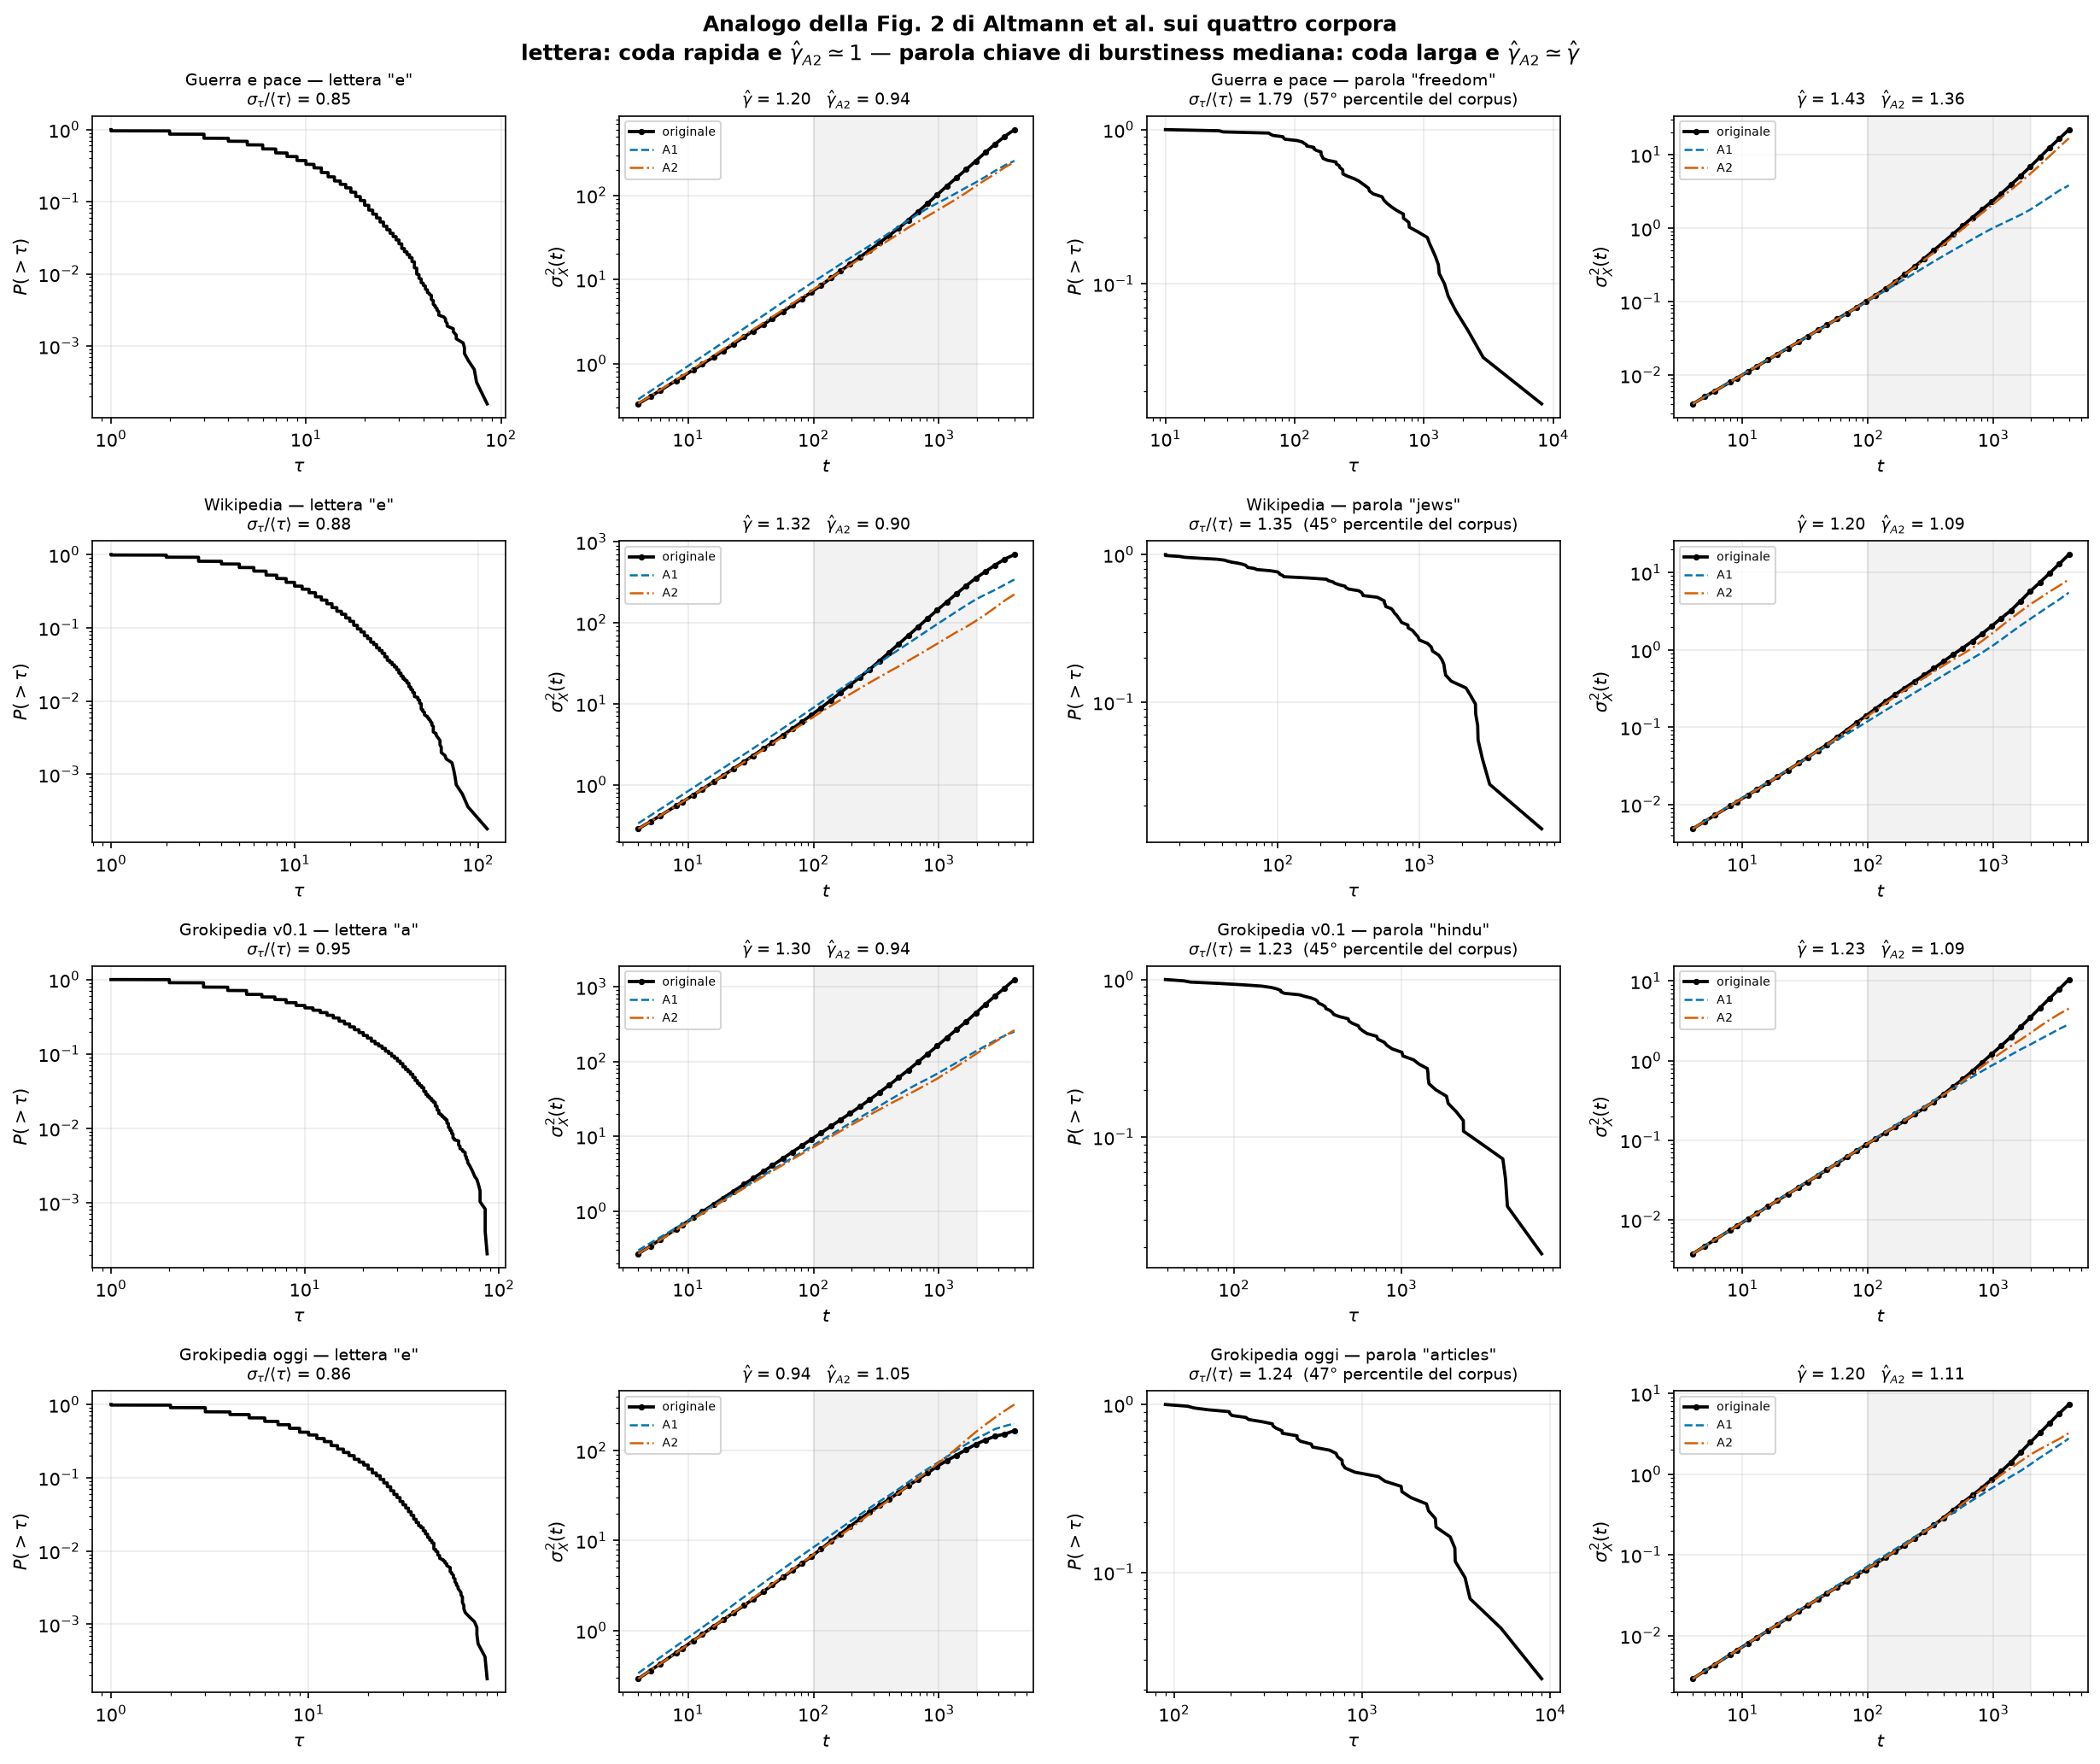
\includegraphics[width=\textwidth]{figure/cap5_altmann_fig2.png}
  \caption{Analogo della Figura~2 di~\cite{altmann2012} sui quattro corpora. Una
  riga per corpus; a sinistra la lettera più frequente del documento, a destra
  la parola chiave di burstiness mediana del corpus fra quelle con almeno
  \num{40} occorrenze, con il suo percentile indicato sopra il pannello. Per
  ciascuna, la distribuzione cumulata degli intervalli $P(>\tau)$ e la crescita
  della varianza del conteggio $\sigma_X^2(t)$, con le curve dei due null model
  del §\ref{sec:null} e la finestra di fit ombreggiata. La lettera ha coda
  rapida e $\hat\gamma_{A2} \simeq 1$; la parola di contenuto ha coda larga e
  $\hat\gamma_{A2}$ prossimo a $\hat\gamma$.}
  \label{fig:altmann-fig2}
\end{figure}

\paragraph{Il soggetto della voce non è una parola di contenuto.}
La parola chiave più ricorrente di un articolo enciclopedico, quella che il
criterio scartato sopra avrebbe selezionato, si comporta in modo opposto a
quello che il §\ref{sec:origini} prevede per il suo livello linguistico. Nella
voce \emph{Alexander the Great} di Wikipedia la parola \emph{alexander} ha
$\sigma_\tau/\langle\tau\rangle = 0.78$; in \emph{Sigmund Freud} di Grokipedia
\emph{freud} ha $0.72$. Sono valori sotto il limite poissoniano, cioè
distribuzioni \emph{più regolari del caso}, mentre la lettera \emph{e} negli
stessi testi dà $0.84$. Il confronto con la lettera non va però fatto sul valore
grezzo. Per un processo casuale in tempo discreto
$\sigma_\tau/\langle\tau\rangle$ non vale esattamente uno, ma tanto meno quanto
più corti sono gli intervalli: il null model A1, applicato alla stessa frequenza
della sequenza osservata, restituisce $0.95$ per la lettera \emph{e}, che ricorre
ogni dieci caratteri, e $1.00$ per una parola chiave, che ricorre ogni
duecento.

\paragraph{Il riferimento casuale dipende dalla frequenza.}
La ragione di quel $0.95$ è che gli intervalli sono numeri interi positivi. Se
le occorrenze sono collocate a caso con probabilità $f$ per carattere, la
distanza fra due consecutive è geometrica, e per la geometrica si ha
$\sigma_\tau/\langle\tau\rangle = \sqrt{1-f}$: il valore tende a uno solo nel
limite di eventi rari. Con $f = 1/10$, la frequenza della lettera \emph{e}, si
ottiene $0.949$; con $f = 1/200$, la frequenza tipica di una parola chiave,
$0.997$. Il valore poissoniano di riferimento non è dunque lo stesso ai due
livelli, ed è più basso proprio dove gli eventi sono più fitti. Confrontare
\emph{alexander} e la lettera \emph{e} sui valori grezzi significherebbe
attribuire alla struttura del testo una differenza che è invece un effetto
della sola frequenza.

Rapportando ciascuna misura al proprio valore casuale l'effetto si toglie, e
resta $0.78$ per \emph{alexander} contro $0.88$ per la lettera: il soggetto
della voce è più regolare di una lettera anche dopo aver tolto l'effetto della
frequenza, e la differenza fra i due, lungi dall'essere prodotta dalla
normalizzazione, ne esce accentuata.

\paragraph{Perché il soggetto si comporta così.}
La ragione è che in prosa enciclopedica il soggetto non è un tema fra altri,
che alterna presenza e assenza lungo il testo, ma il tema unico: compare come soggetto grammaticale di quasi ogni
periodo, e i suoi intervalli ereditano allora la statistica della lunghezza
delle frasi anziché quella dell'alternanza tematica. La verifica è diretta.
Nei sei articoli esaminati il soggetto ricorre una volta ogni $1.4$--$1.7$
frasi, con lo stesso valore in Wikipedia e in Grokipedia. I suoi intervalli sono
quindi lunghezze di frase, e ne ereditano la variabilità: le
lunghezze di frase di quegli articoli hanno
$\sigma_\tau/\langle\tau\rangle$ fra $0.33$ e $0.73$, e il soggetto della voce
si colloca poco sopra, fra $0.54$ e $0.78$, comunque sotto l'unità che
segnerebbe l'assenza di struttura. Per confronto, \emph{natásha} in un segmento
di \emph{Guerra e pace} ricorre una volta ogni $5.1$ frasi e ha
$\sigma_\tau/\langle\tau\rangle = 3.24$: lì la ricorrenza non segue il ritmo del
periodo ma l'alternanza delle scene.

Il soggetto della voce funziona quindi da marcatore sintattico e non semantico,
e la sua ricorrenza è governata dal ritmo del periodo, non dalla persistenza di
un argomento. Non è un difetto della misura ma un tratto del genere
enciclopedico, e va tenuto presente nel confrontare la burstiness lessicale fra
generi diversi: è la ragione per cui la parola mostrata nella
Figura~\ref{fig:altmann-fig2} viene scelta sulla mediana e non sul massimo.

% ---------------------------------------------------------------------
\section{Il divario si apre al livello lessicale}
\label{sec:appaiato}

L'appaiamento per titolo permette un test più stringente del confronto fra
medie. Confrontare la media di Wikipedia con quella di Grokipedia lascia
aperta l'obiezione che le due medie siano calcolate su argomenti diversi, e
che la differenza rifletta il contenuto anziché la scrittura. Il test appaiato
la chiude: per ciascuna delle \num{39} voci, che nei due corpora tratta lo
stesso argomento, si calcola la differenza fra il valore di Grokipedia e
quello di Wikipedia, e si verifica con il test dei ranghi segnati di Wilcoxon
che la mediana di quelle \num{39} differenze sia diversa da zero. Il test è
non parametrico, quindi non assume che le differenze siano distribuite
normalmente, assunzione che con \num{39} osservazioni e distribuzioni
asimmetriche non sarebbe difendibile.

Il test dà, per la versione attuale di Grokipedia,
$-0.167$ sulle parole chiave e $-0.010$ sulle lettere; ai due livelli intermedi
le differenze valgono $-0.037$ per le parole funzione e $-0.157$ per i controlli
appaiati, tutte con significatività inferiore a $10^{-2}$. La versione v0.1 dà
$-0.012$, $-0.039$, $-0.116$ e $-0.133$.

I quattro numeri vanno letti come una scala. Alle lettere Grokipedia e
Wikipedia distano un centesimo di unità di burstiness, cioè circa l'uno per
cento del valore misurato: a quel livello i due corpora sono, in pratica, lo
stesso testo. Alle parole funzione la distanza quadruplica, ma resta piccola in
termini relativi. Ai due livelli lessicali passa a circa sedici centesimi, oltre
un decimo del valore misurato e più di un ordine di grandezza sopra il livello
delle lettere.

La scala ha però un solo gradino, non tre. La differenza fra i livelli
sub-lessicali e quelli lessicali è netta; quella fra i due livelli lessicali non
esiste: $-0.157$ sui controlli a frequenza appaiata contro $-0.167$ sulle parole
chiave sono lo stesso numero. Il testo generato non perde dunque le parole di
contenuto più di quanto perda le altre parole della stessa frequenza. Ciò che i
dati sostengono è che riproduca le regolarità dei livelli bassi e abbassi
uniformemente la burstiness a livello di parola, non che perda selettivamente la
persistenza tematica.

\paragraph{Il divario alla lunghezza di controllo.}
\label{sec:robustezza-neff}
L'intera catena è stata ripetuta a $N_{\mathrm{eff}} = \num{80000}$ caratteri,
lunghezza a cui sopravvivono \num{35} delle \num{39} terne; per isolare
l'effetto della finestra, i valori a \num{60000} sono ricalcolati sulle stesse
\num{35}. Alle lettere e alle parole funzione il divario appaiato è stabile, da
$-0.010$ a $-0.011$ e da $-0.037$ a $-0.045$; ai due livelli lessicali si separa
in direzioni opposte, con i controlli appaiati da $-0.164$ a $-0.195$ e le parole
chiave da $-0.167$ a $-0.130$, quest'ultima con significatività che scende a
$p = 0.027$. Alla lunghezza maggiore il divario sulle parole chiave è dunque
\emph{minore} di quello sui controlli appaiati. Ciò che risulta robusto è il
salto dal livello sub-lessicale a quello lessicale; l'ulteriore crescita fino
alle parole chiave non lo è. Anche l'esponente di coda è instabile fra le due
lunghezze, da $2.19$ a $2.50$ su Grokipedia e da $2.37$ a $2.25$ su Wikipedia,
coerentemente con l'avvertenza del §\ref{sec:coda-risultati}.

La Figura~\ref{fig:altmann-fig3} riporta le stesse sequenze nel piano che
\cite{altmann2012} usa per la propria Figura~3: la burstiness in ascissa e
l'esponente di correlazione in ordinata, un punto per sequenza, con un simbolo
diverso per livello linguistico. La gerarchia vi si legge come una disposizione
spaziale: le lettere, gli spazi e le vocali si addensano in una colonna stretta
attorno a $\sigma_\tau/\langle\tau\rangle \simeq 0.5$, le parole funzione e i
controlli appaiati occupano la regione centrale, le parole chiave si spingono a
destra e in alto. È la stessa gerarchia dei paragrafi precedenti, vista tutta
insieme invece che un livello alla volta.

Il piano rende però visibile anche una proprietà che i confronti per livello
non mostrano, e che è l'osservazione centrale di quel lavoro: l'angolo in
basso a destra è vuoto. Non esistono, cioè, sequenze molto \emph{bursty} e
insieme poco correlate. Sui quattro corpora di questa tesi la regolarità si
quantifica così: delle $451$ sequenze con $\sigma_\tau/\langle\tau\rangle >
1.5$, soltanto $17$, il $3.8\%$, hanno $\hat\gamma < 1.1$, e fra quelle con
burstiness superiore a $2$ l'esponente non scende mai sotto $1.05$. L'angolo
opposto, invece, è popolato: delle $3500$ sequenze sotto il valore poissoniano
$\sigma_\tau/\langle\tau\rangle = 1$, il $15.9\%$ ha $\hat\gamma > 1.2$.

L'asimmetria fra i due angoli è la firma di una relazione a senso unico. La
burstiness produce correlazione, come mostra la~\eqref{eq:eq4}, e una sequenza
con vuoti lunghi non può quindi risultare scorrelata; il viceversa non vale,
perché la correlazione può venire anche dall'ordine degli intervalli e
manifestarsi senza alcuna coda pesante. La correlazione di rango fra le due
quantità è positiva e significativa in tutti e quattro i corpora, da $+0.22$ su
Wikipedia a $+0.36$ sul romanzo. Il meccanismo descritto in~\cite{altmann2012}
sui romanzi si ritrova dunque identico nella prosa enciclopedica e in quella
generata, ed è un risultato indipendente dal divario misurato sopra: riguarda
come le due grandezze si legano fra loro, non quanto valgano.

\begin{figure}[htbp]
  \centering
  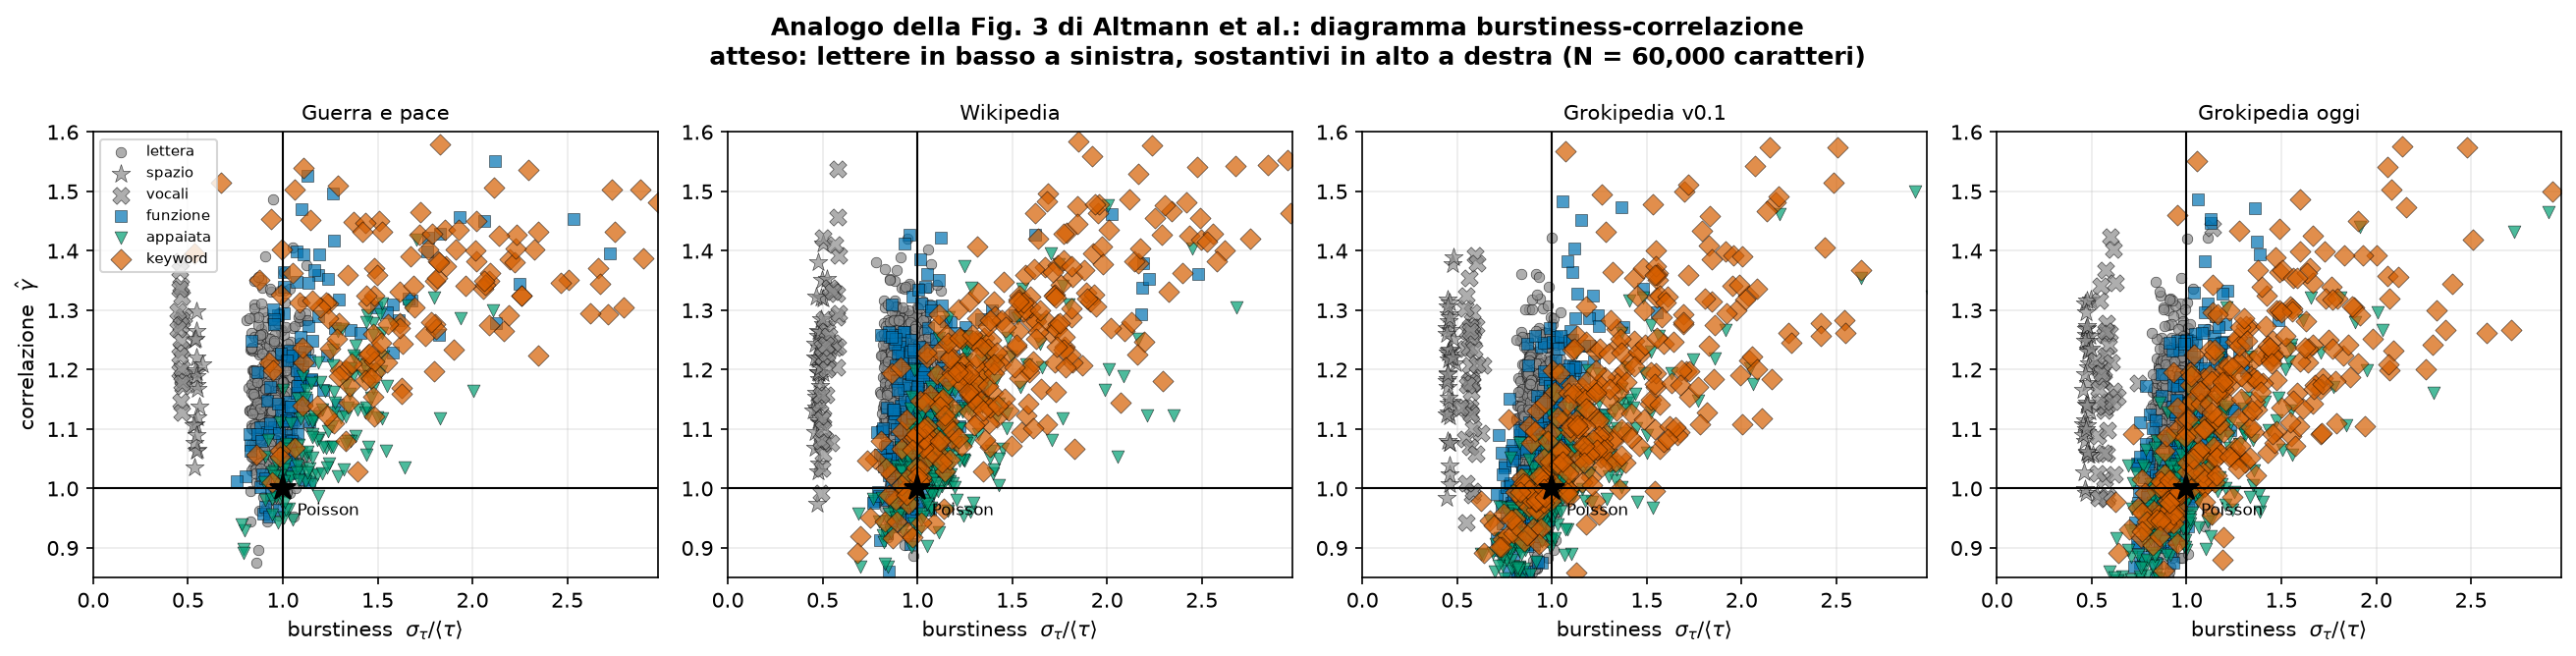
\includegraphics[width=\textwidth]{figure/cap5_altmann_fig3.png}
  \caption{Analogo della Figura~3 di~\cite{altmann2012}: diagramma
  burstiness--correlazione sui quattro corpora, un punto per sequenza. Oltre ai
  quattro livelli usati nel resto del capitolo sono riportati i due livelli
  sub-lessicali tenuti come diagnostica, gli spazi e le vocali. Le linee nere
  segnano il processo di Poisson,
  $\sigma_\tau/\langle\tau\rangle = 1$ e $\hat\gamma = 1$. L'angolo in basso a
  destra è praticamente vuoto in tutti e quattro i corpora: sequenze molto
  bursty e insieme poco correlate non si osservano.}
  \label{fig:altmann-fig3}
\end{figure}

\paragraph{I due quadranti che restano.} La lettura del piano fatta finora
riguarda la diagonale: l'angolo in basso a destra vuoto e quello in alto a
sinistra popolato. Gli altri due separano però i corpora meglio di qualunque
media, e la Figura~\ref{fig:quadranti} li riporta separatamente. Fra le parole
chiave, l'angolo in alto a destra è la posizione canonica
di~\cite{altmann2012}, quella in cui la sequenza è insieme bursty e correlata.
Vi ricade il $91.4\%$ delle sequenze di \emph{Guerra e pace} e l'$87.5\%$ di
quelle di Wikipedia, ma solo il $74.0\%$ di Grokipedia v0.1 e il $77.3\%$
della versione attuale. La differenza finisce quasi interamente nell'angolo
opposto, in basso a sinistra, dove la parola è più regolare di un processo di
Poisson e insieme priva di correlazione a lungo raggio: $0\%$ sul romanzo,
$5.1\%$ su Wikipedia, $15.4\%$ su Grokipedia v0.1 e $14.3\%$ sulla versione
attuale. Una parola chiave generata su sette si trova dunque nell'angolo
opposto a quello canonico, contro una su venti in Wikipedia. Il test appaiato
sulle \num{39} voci conferma che non è un effetto di composizione del
campione: la quota di parole chiave in basso a sinistra cresce in $21$ e $22$
voci su $39$, con differenza mediana $+0.143$ e $p < 10^{-3}$ per entrambe le
versioni.

Due controlli escludono le spiegazioni strumentali. Il null model A1
restituisce $\hat\gamma = 0.983$ in tutti e quattro i corpora, identico alla
terza cifra, quindi la soglia $\hat\gamma = 1$ non è tarata diversamente da un
corpus all'altro; il valore calibrato non è però esattamente uno, cosicché la
soglia è lievemente generosa verso il lato correlato, allo stesso modo per
tutti. E la quota di parole in basso a sinistra resta più alta in Grokipedia
dentro quattro fasce di frequenza su cinque, da $0.159$ contro $0.050$ per le
parole con $26$--$35$ occorrenze a $0.303$ contro $0.076$ per quelle con più di
$80$. Fa eccezione la fascia più bassa, $15$--$25$ occorrenze, dove il rapporto
si inverte, $0.065$ contro $0.200$; lì però le parole chiave di Wikipedia sono
dieci in tutto e la quota è stimata su di esse. Il divario non dipende quindi
dal fatto che le parole chiave di Wikipedia siano più frequenti, salvo nella
fascia in cui il confronto ha meno appoggio.

Guardare dentro il quadrante non rivela più un gruppo omogeneo. Separando le
parole che compaiono nel titolo della voce dalle altre, le $14$ di Wikipedia si
dividono a metà, e le $39$ di Grokipedia si dividono in $18$ soggetti di voce e
$21$ altre parole, prevalentemente aggettivi generici: \emph{economic} in cinque
voci, \emph{military} in tre, \emph{urban} in due. Sono concentrazioni modeste,
e soprattutto non sono più quelle che la lista di parole funzione originaria
lasciava passare: con quella lista, il quadrante conteneva \emph{like} in dodici
voci, \emph{amid} in nove e \emph{including} in sei, cioè i connettivi che
costituiscono il vizio stilistico più evidente del testo generato. Quei termini
sono ora classificati come parole funzione, che è ciò che sono, e il
§\ref{sec:effetto-stoplist} misura quanto la loro presenza fra le parole chiave
alterasse i risultati.

\begin{figure}[htbp]
  \centering
  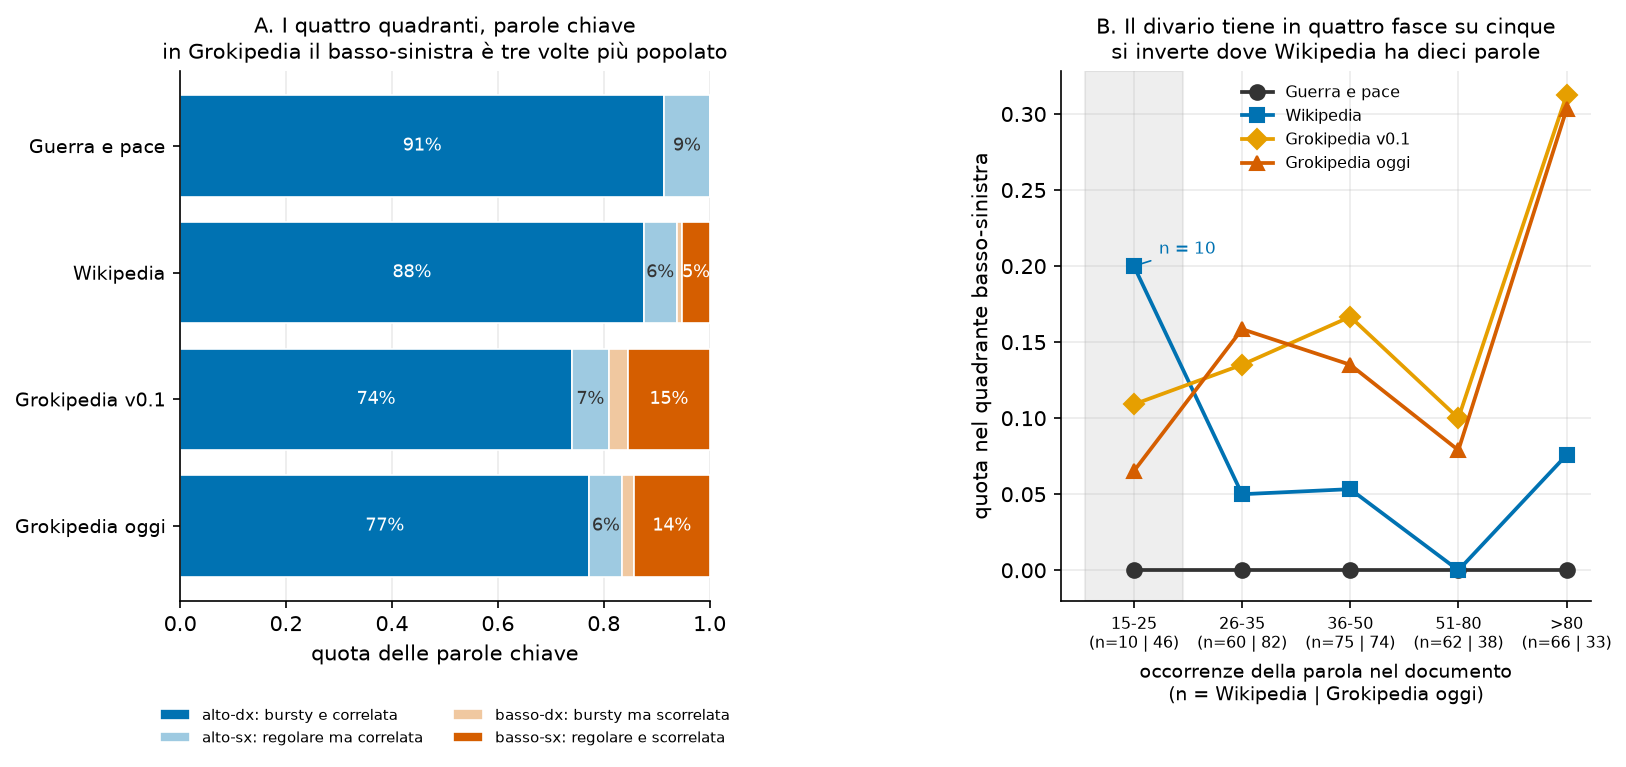
\includegraphics[width=\textwidth]{figure/cap5_quadranti.png}
  \caption{Lettura per quadranti del piano della
  Figura~\ref{fig:altmann-fig3}, sulle sole parole chiave. A: composizione per
  quadrante, un corpus per riga; le quote sotto il $5\%$ non sono etichettate. B:
  quota di parole chiave nel quadrante in basso a sinistra, separando le parole
  per numero di occorrenze nel documento; sotto ciascuna fascia è indicato
  quante parole chiave vi cadono in Wikipedia e in Grokipedia. Il divario tiene
  in quattro fasce su cinque e si inverte nella più bassa, dove Wikipedia ne ha
  dieci in tutto e la fascia è ombreggiata per segnalarlo.}
  \label{fig:quadranti}
\end{figure}

\paragraph{Un effetto di scala da neutralizzare.} Le voci di Grokipedia hanno
frasi sensibilmente
più lunghe di quelle di Wikipedia: $4.38$ frasi ogni mille caratteri contro
$6.92$. Poiché in questo capitolo il tempo è contato in caratteri, la scala
degli intervalli $\tau$ non è la stessa nei due corpora, e un testo con frasi
più lunghe tende ad avere intervalli più lunghi anche a parità di struttura
tematica. Il coefficiente di variazione è un rapporto e non risente di una
dilatazione uniforme dell'asse, ma la dilatazione qui non è uniforme, perché
agisce solo sui livelli definiti su unità linguistiche. Il
§\ref{sec:entropia-intervalli} introduce la misura che elimina il problema;
fino a quel punto il divario va considerato provvisorio.

Il riferimento letterario, infine, non è appaiato per argomento con nessuno dei
tre corpora enciclopedici: entra nei confronti come livello medio e non nei test
appaiati.

% ---------------------------------------------------------------------
\section{Quale meccanismo genera la correlazione}
\label{sec:decomposizione}

Sapere che un testo ha correlazioni a lungo raggio non dice da dove esse
vengano. Il §\ref{sec:null} ha introdotto i due null model che separano le due
origini possibili e la quota di burstiness $q$ della~\eqref{eq:quota}, che vale
circa uno quando la correlazione è interamente spiegata dalla distribuzione
degli intervalli, e circa zero quando è invece l'ordine in cui le occorrenze si
susseguono a produrla.

Il primo pannello della Figura~\ref{fig:decomposizione} riporta $q$ ai quattro
livelli. Sulle lettere il valore è negativo in tutti e quattro i corpora, da
$-0.06$ su Wikipedia a $-0.19$ su Grokipedia v0.1: le lettere sono correlate,
come mostra il $\hat\gamma$ maggiore di uno, ma non sono \emph{bursty}, e la
correlazione viene interamente dall'ordine. Sulle parole chiave il valore sale a
$0.89$ sul romanzo, $0.77$ su Wikipedia, $0.70$ sulla v0.1 e $0.74$ sulla
versione attuale di Grokipedia: qui quasi tutta la correlazione è già contenuta nella
distribuzione degli intervalli. I due livelli intermedi interpolano fra i due
regimi in modo ordinato.

La dissociazione fra il livello dei caratteri e quello del contenuto, che
in~\cite{altmann2012} è osservata su romanzi, si ritrova quindi identica nella
prosa enciclopedica e anche nella prosa generata. Il secondo pannello mostra la
stessa cosa in termini di esponenti: le curve piene sono $\hat\gamma$ e quelle
tratteggiate $\hat\gamma_{A2}$, e la distanza verticale fra le due è il
contributo dell'ordine delle occorrenze. Sulle lettere le due curve sono
separate e la tratteggiata sta all'unità; sulle parole chiave si avvicinano e
salgono insieme.

I valori dei tre corpora enciclopedici sono però troppo vicini perché la
differenza sia interpretabile: fra Wikipedia e Grokipedia vale $0.03$ alla
lunghezza di lavoro e cambia segno a quella di controllo del
§\ref{sec:robustezza-neff}. I dati non consentono quindi di attribuire ai due
corpora un'origine diversa della correlazione, ma soltanto un'intensità diversa.

Sulla riga dei controlli appaiati per Grokipedia, infine, la quota è stimabile
solo su $6$ documenti su $39$ per la versione v0.1 e su $8$ per quella
attuale. La ragione non è un difetto della stima ma la grandezza stessa: $q$
ha $\hat\gamma - 1$ al denominatore, e viene calcolata soltanto dove quel
denominatore supera $0.05$, perché sotto quella soglia il rapporto è dominato
dall'errore. A quel livello i documenti di Grokipedia hanno $\hat\gamma$
mediano pari a $1.003$ per la v0.1 e $1.015$ per la versione attuale, contro
$1.091$ di Wikipedia: le loro sequenze di controllo sono essenzialmente
scorrelate, e non c'è alcuna correlazione da decomporre nelle due origini.
L'esclusione è quindi essa stessa un dato, perché è il livello in cui il testo
generato si avvicina di più al caso, ma il valore di $q$ che sopravvive sui
pochi documenti restanti riguarda proprio quelli in cui una correlazione c'è,
e non va letto come una misura del corpus.

\begin{figure}[htbp]
  \centering
  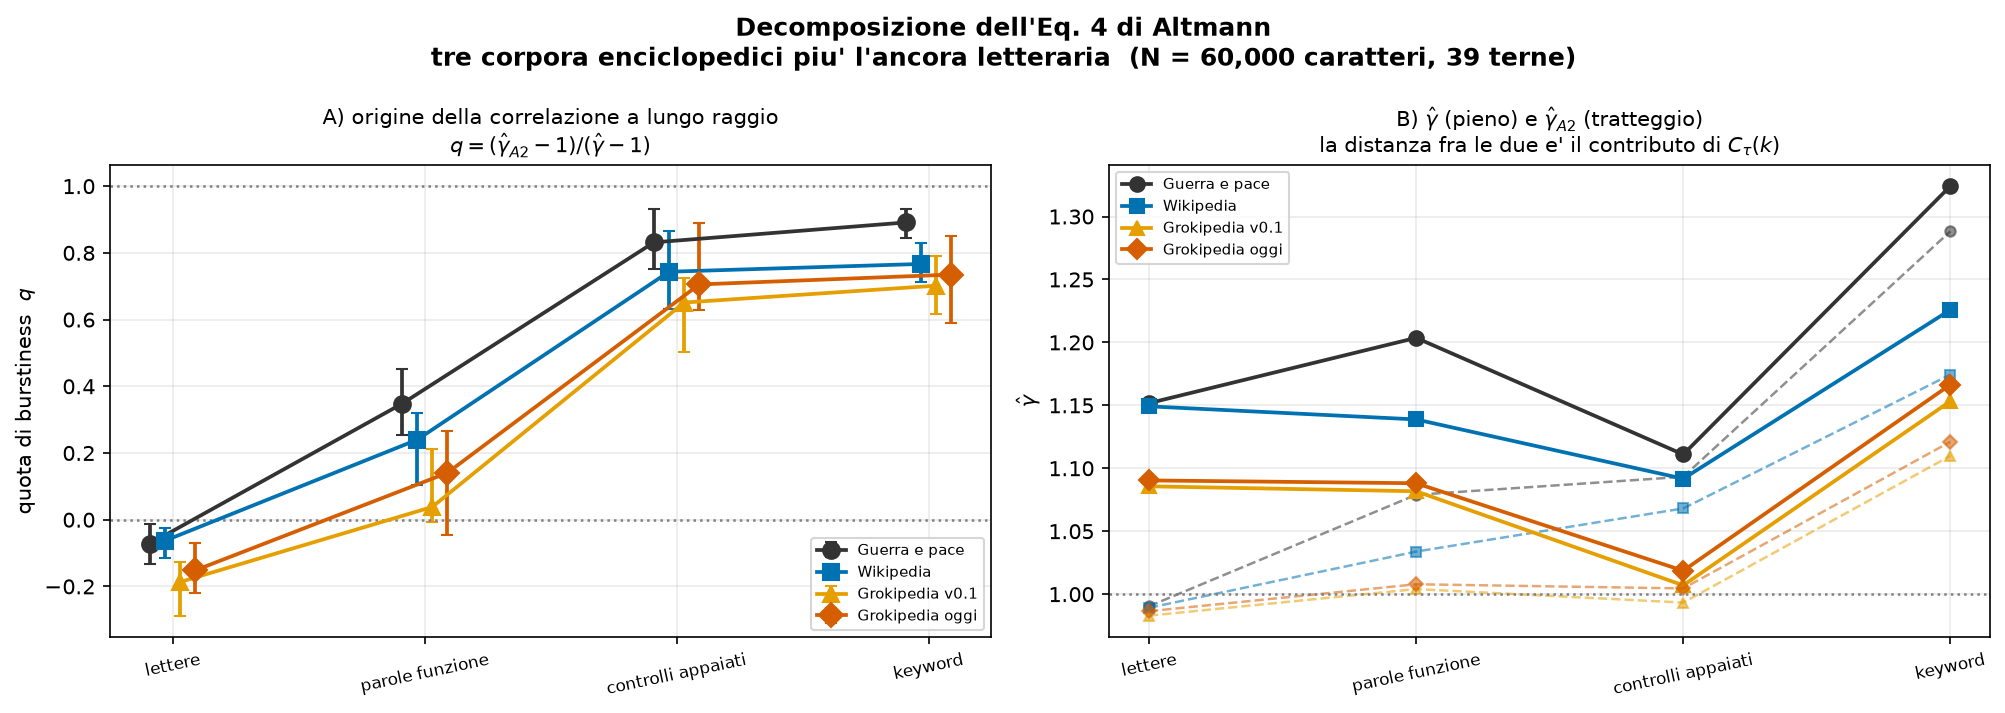
\includegraphics[width=\textwidth]{figure/cap5_decomposizione_eq4.png}
  \caption{Decomposizione della correlazione nelle sue due origini. A: quota
  $q$ della~\eqref{eq:quota} ai quattro livelli linguistici, con intervalli di
  confidenza; $q \simeq 0$ indica correlazione dovuta all'ordine delle
  occorrenze, $q \simeq 1$ correlazione dovuta alla distribuzione degli
  intervalli. B: esponente $\hat\gamma$ (linea piena) e $\hat\gamma_{A2}$
  (tratteggiata) agli stessi livelli; la distanza fra le due curve è il
  contributo della correlazione fra intervalli successivi.}
  \label{fig:decomposizione}
\end{figure}

% ---------------------------------------------------------------------
\section{La coda della distribuzione degli intervalli}
\label{sec:coda-risultati}

Il §\ref{sec:coda} ha osservato che la relazione fra esponente di coda e
esponente di correlazione, nella forma in cui compare in~\cite{altmann2012},
presuppone una distribuzione degli intervalli di cui la coda non viene misurata
ma assunta. Qui la coda viene stimata direttamente, adottando il modello
troncato
\begin{equation}
  p(\tau) \;\sim\; \tau^{-\mu}\,e^{-\tau/\tau_c}
  \label{eq:coda-troncata}
\end{equation}
e determinando $\mu$ e $\tau_c$ per massima verosimiglianza, con intervalli di
confidenza di profilo.

L'analisi della coda comprende, oltre ai quattro livelli usati nel resto del
capitolo, due livelli sub-lessicali aggiuntivi tenuti come diagnostica, le
vocali e gli spazi, per un totale di ventiquattro celle. Il primo risultato
riguarda la forma stessa della distribuzione: il confronto di verosimiglianza
fra la~\eqref{eq:coda-troncata} e una legge di potenza pura rifiuta
quest'ultima in tutte e ventiquattro, con significatività numericamente
indistinguibile da zero. La coda esiste, ma è tagliata.

Il primo pannello della Figura~\ref{fig:coda} riporta $\mu$ ai quattro livelli.
La banda verde segna la regione $2 < \mu < 3$ entro cui la~\eqref{eq:eq8} è
derivata assumendo una legge di potenza pura. Che le stime vi cadano dentro o
fuori non dice nulla sulla convergenza dei momenti: nella
~\eqref{eq:coda-troncata} il taglio li rende finiti per qualunque $\mu$, e il
rifiuto della potenza pura in tutte e ventiquattro le celle toglie il
presupposto sotto cui la banda avrebbe quel significato. Resta un riferimento
utile perché è la regione in cui il paper colloca il proprio valore assunto.
I simboli grigi segnalano le celle in cui il fit degenera in un
esponenziale puro e $\mu$ non è interpretabile, e le linee di collegamento le
saltano. Sono sette celle su sedici: tutti e quattro i corpora sul livello delle
lettere, e i tre corpora enciclopedici su quello delle parole funzione.

Alle parole funzione il romanzo è l'unico dei quattro il cui fit non degenera,
con $\tau_c = 5.3$ contro $1.7$--$1.9$: le sue parole funzione conservano un
tratto di coda a legge di potenza che negli altri tre corpora non esiste, e a
quel livello il coefficiente di variazione dà lo stesso quadro, $1.19$ contro
valori fra $0.97$ e $1.03$ indistinguibili da un processo di Poisson.

Sarebbe naturale leggerlo come una differenza di genere, e il controllo non lo
conferma. Ripetendo la stessa procedura sui tre romanzi inglesi impiegati come
controllo in questo capitolo, il fit sulle parole funzione degenera su
\emph{Moby Dick} ($\tau_c = 1.7$, esattamente il valore dei corpora
enciclopedici) e su \emph{David Copperfield} ($\tau_c = 2.8$), e sopravvive per
poco su \emph{Middlemarch} ($\tau_c = 3.2$); il coefficiente di variazione dà
$1.03$, $1.09$ e $1.08$, cioè valori compresi fra Wikipedia e
\emph{Guerra e pace} e nel primo caso identici a quelli enciclopedici. A questo
livello l'eccezione è quindi del testo e non del genere, come il
§\ref{sec:tre-corpora} osserva anche sul livello delle parole chiave. Il confronto fra i quattro
corpora resta perciò leggibile soltanto sulle parole chiave, dove i valori
stanno fra $1.76$ e $2.37$; sui controlli appaiati tutti e quattro i fit sono al
limite della degenerazione e gli intervalli di confidenza superano l'unità di
ampiezza.

Il confronto con~\cite{altmann2012} chiude qui un cerchio. In quel lavoro $\mu$
non viene stimato ma assunto: per costruire il limite inferiore di $\hat\gamma$
della propria Figura~3 gli autori adottano il valore $\mu = 2.4$. La stima
diretta condotta qui lo colloca dentro l'intervallo di confidenza di tutti e tre
i corpora enciclopedici, e a tre centesimi dal valore centrale di Wikipedia. Il
parametro che quel lavoro doveva postulare risulta dunque misurabile, e il
valore postulato corretto. Il confronto è legittimo perché $\mu$ designa in
entrambi i casi la pendenza della coda nella regione in cui la legge di potenza
vale; ciò che cambia è che qui quella regione è delimitata da un $\tau_c$
stimato anziché estesa all'infinito, e il capoverso seguente misura quanto la
differenza di modello sposti il numero.

Il corpus letterario fa eccezione, con $\mu = 1.76$ e intervallo di confidenza
$[1.40, 2.08]$, e su questo servono due precisazioni, perché il valore cade
sotto la banda $2 < \mu < 3$ entro cui la~\eqref{eq:eq8} è derivata. La prima
è che non è una particolarità di \emph{Guerra e pace}: ripetendo l'intera
procedura su tre altri romanzi inglesi, segmentati e misurati allo stesso
modo, si ottiene $1.51$ su \emph{Moby Dick}, $2.10$ su \emph{Middlemarch} e
$1.96$ su \emph{David Copperfield}, tutti sotto il valore di Wikipedia a ogni
quantile di $x_{\min}$ dall'ottantesimo in su. È un tratto della prosa
letteraria, non del testo scelto, ed è lo stesso fatto che il coefficiente di
variazione registra come burstiness massima: coda più pesante significa
esponente più piccolo.

La seconda è che il valore dipende dal modello con cui lo si stima. Sotto il
modello troncato adottato qui la banda $2 < \mu < 3$ non ha ruolo, perché il
taglio rende media e varianza finite per qualunque $\mu$; sotto il modello a
potenza pura, che è quello di~\cite{altmann2012}, lo stimatore di massima
verosimiglianza sugli stessi dati dà $2.49$ per il corpus letterario, dentro la
banda e a nove centesimi dal valore assunto nel paper. I due numeri non sono in
conflitto: descrivono la stessa coda sotto ipotesi diverse, e la scelta fra le
due è decisa dal rapporto di verosimiglianza, che rifiuta la potenza pura. La
misura non contraddice dunque il valore postulato in quel lavoro; ne circoscrive
il modello.

\begin{figure}[htbp]
  \centering
  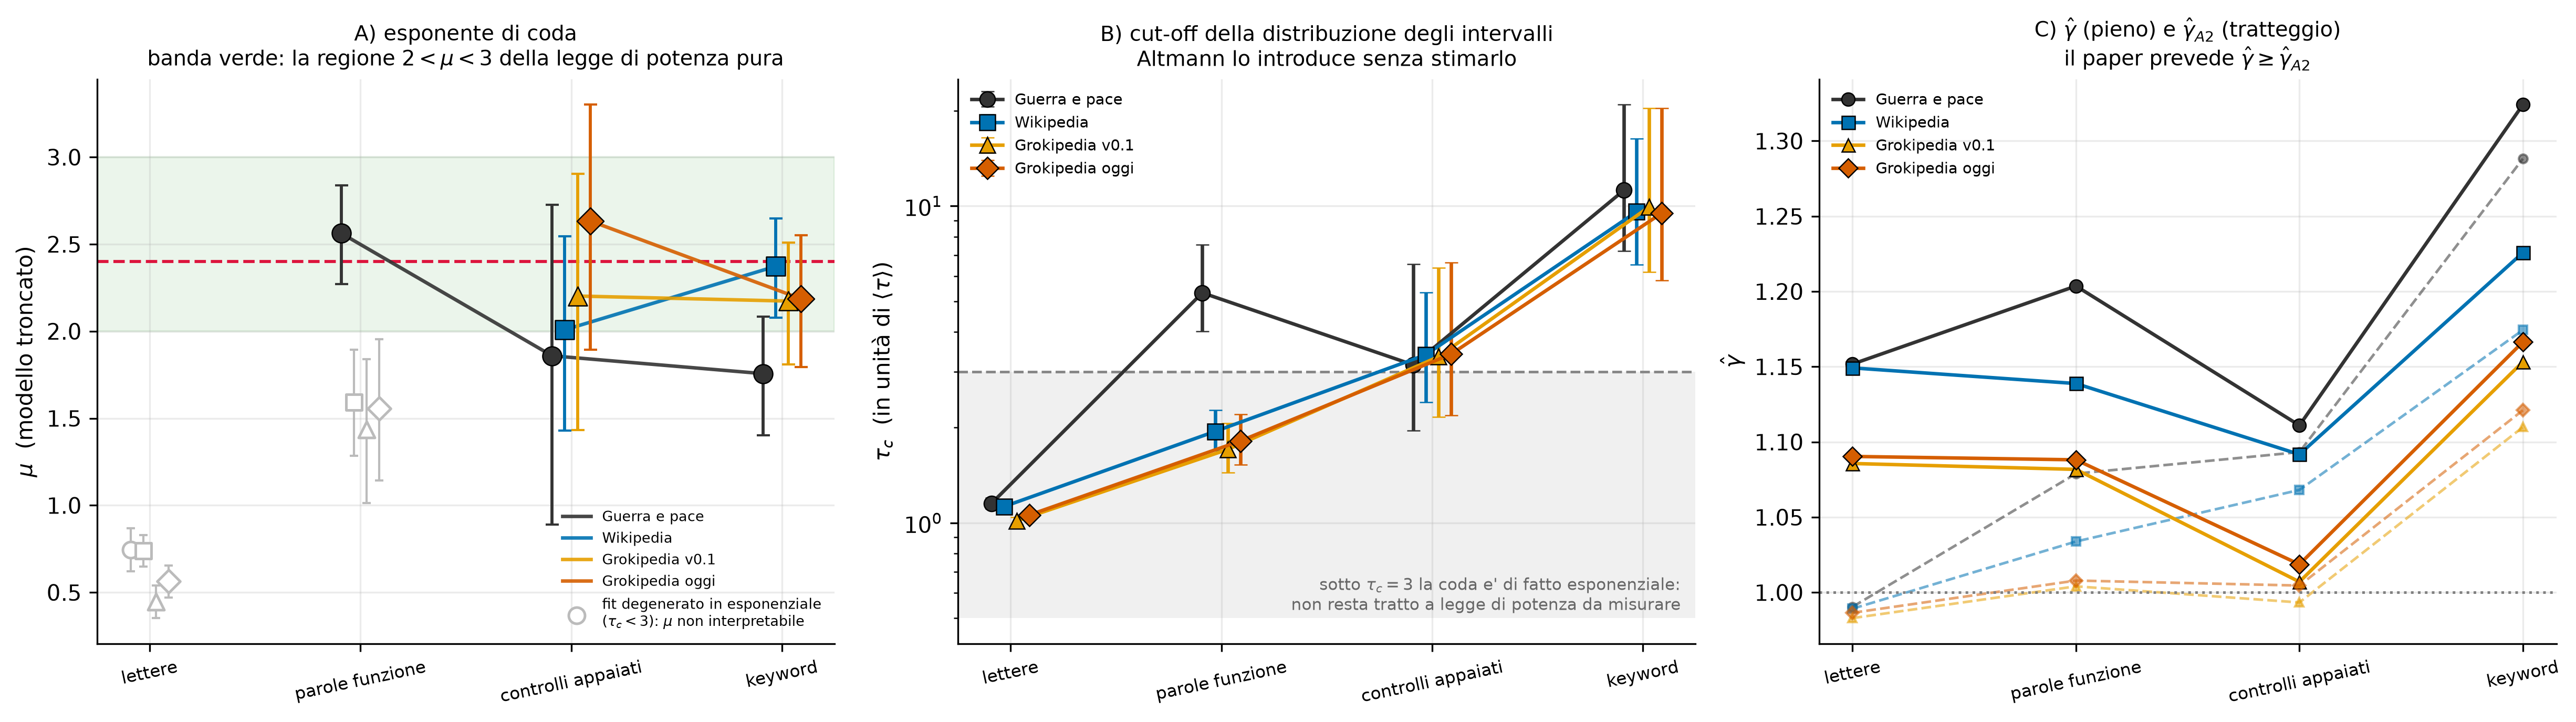
\includegraphics[width=\textwidth]{figure/cap5_esponente_coda.png}
  \caption{Stima diretta della coda della distribuzione degli intervalli. A:
  esponente $\mu$ della~\eqref{eq:coda-troncata} ai quattro livelli, con
  intervalli di confidenza di profilo; la banda verde è la regione $2<\mu<3$ in
  cui è derivata la~\eqref{eq:eq8} per la legge di potenza pura, mentre sotto il
  modello troncato adottato qui i momenti restano finiti per qualunque $\mu$ e
  la banda va letta come riferimento alla letteratura; i simboli grigi sono le
  celle in cui il fit degenera in un esponenziale e $\mu$ non è interpretabile,
  che le linee di collegamento saltano. B: cut-off
  $\tau_c$ agli stessi livelli, in unità dell'intervallo medio e con intervalli
  di confidenza di profilo; sotto la soglia tratteggiata non resta tratto a legge
  di potenza da misurare. C: $\hat\gamma$ (pieno) contro $\hat\gamma_{A2}$
  (tratteggiato) ai quattro livelli. La~\eqref{eq:disug1} è rispettata in tutte
  le celle: la curva piena sta sempre sopra la tratteggiata.}
  \label{fig:coda}
\end{figure}

\paragraph{Perché $\mu$ non serve a confrontare i corpora.}
I quattro valori non vanno però usati per ordinare i corpora, e la
Figura~\ref{fig:verosimiglianza} mostra perché: $\mu$ e $\tau_c$ sono
fortemente correlati, cosicché le regioni di confidenza congiunte sono creste
allungate anziché ellissi compatte e quelle dei tre corpora enciclopedici si
sovrappongono quasi interamente. A ciò si aggiunge la dipendenza dal punto in
cui si decide che la coda cominci: spostando $x_{\min}$ dal settantacinquesimo
al novantacinquesimo percentile $\mu$ passa da $1.65$ a $2.63$ su Wikipedia, una
variazione maggiore di ogni differenza fra corpora, e le curve si incrociano.

Di questa analisi non resta perciò un ordinamento fra corpora. Restano due
risultati, entrambi insensibili alla posizione esatta lungo la cresta: la legge
di potenza pura è rifiutata ovunque, e il cut-off cresce in modo ordinato
salendo nella gerarchia linguistica. Il cut-off è previsto
da~\cite{altmann2012} come conseguenza della discesa lungo quella stessa
gerarchia, e la sua esistenza è qui verificata invece che assunta.

\begin{figure}[htbp]
  \centering
  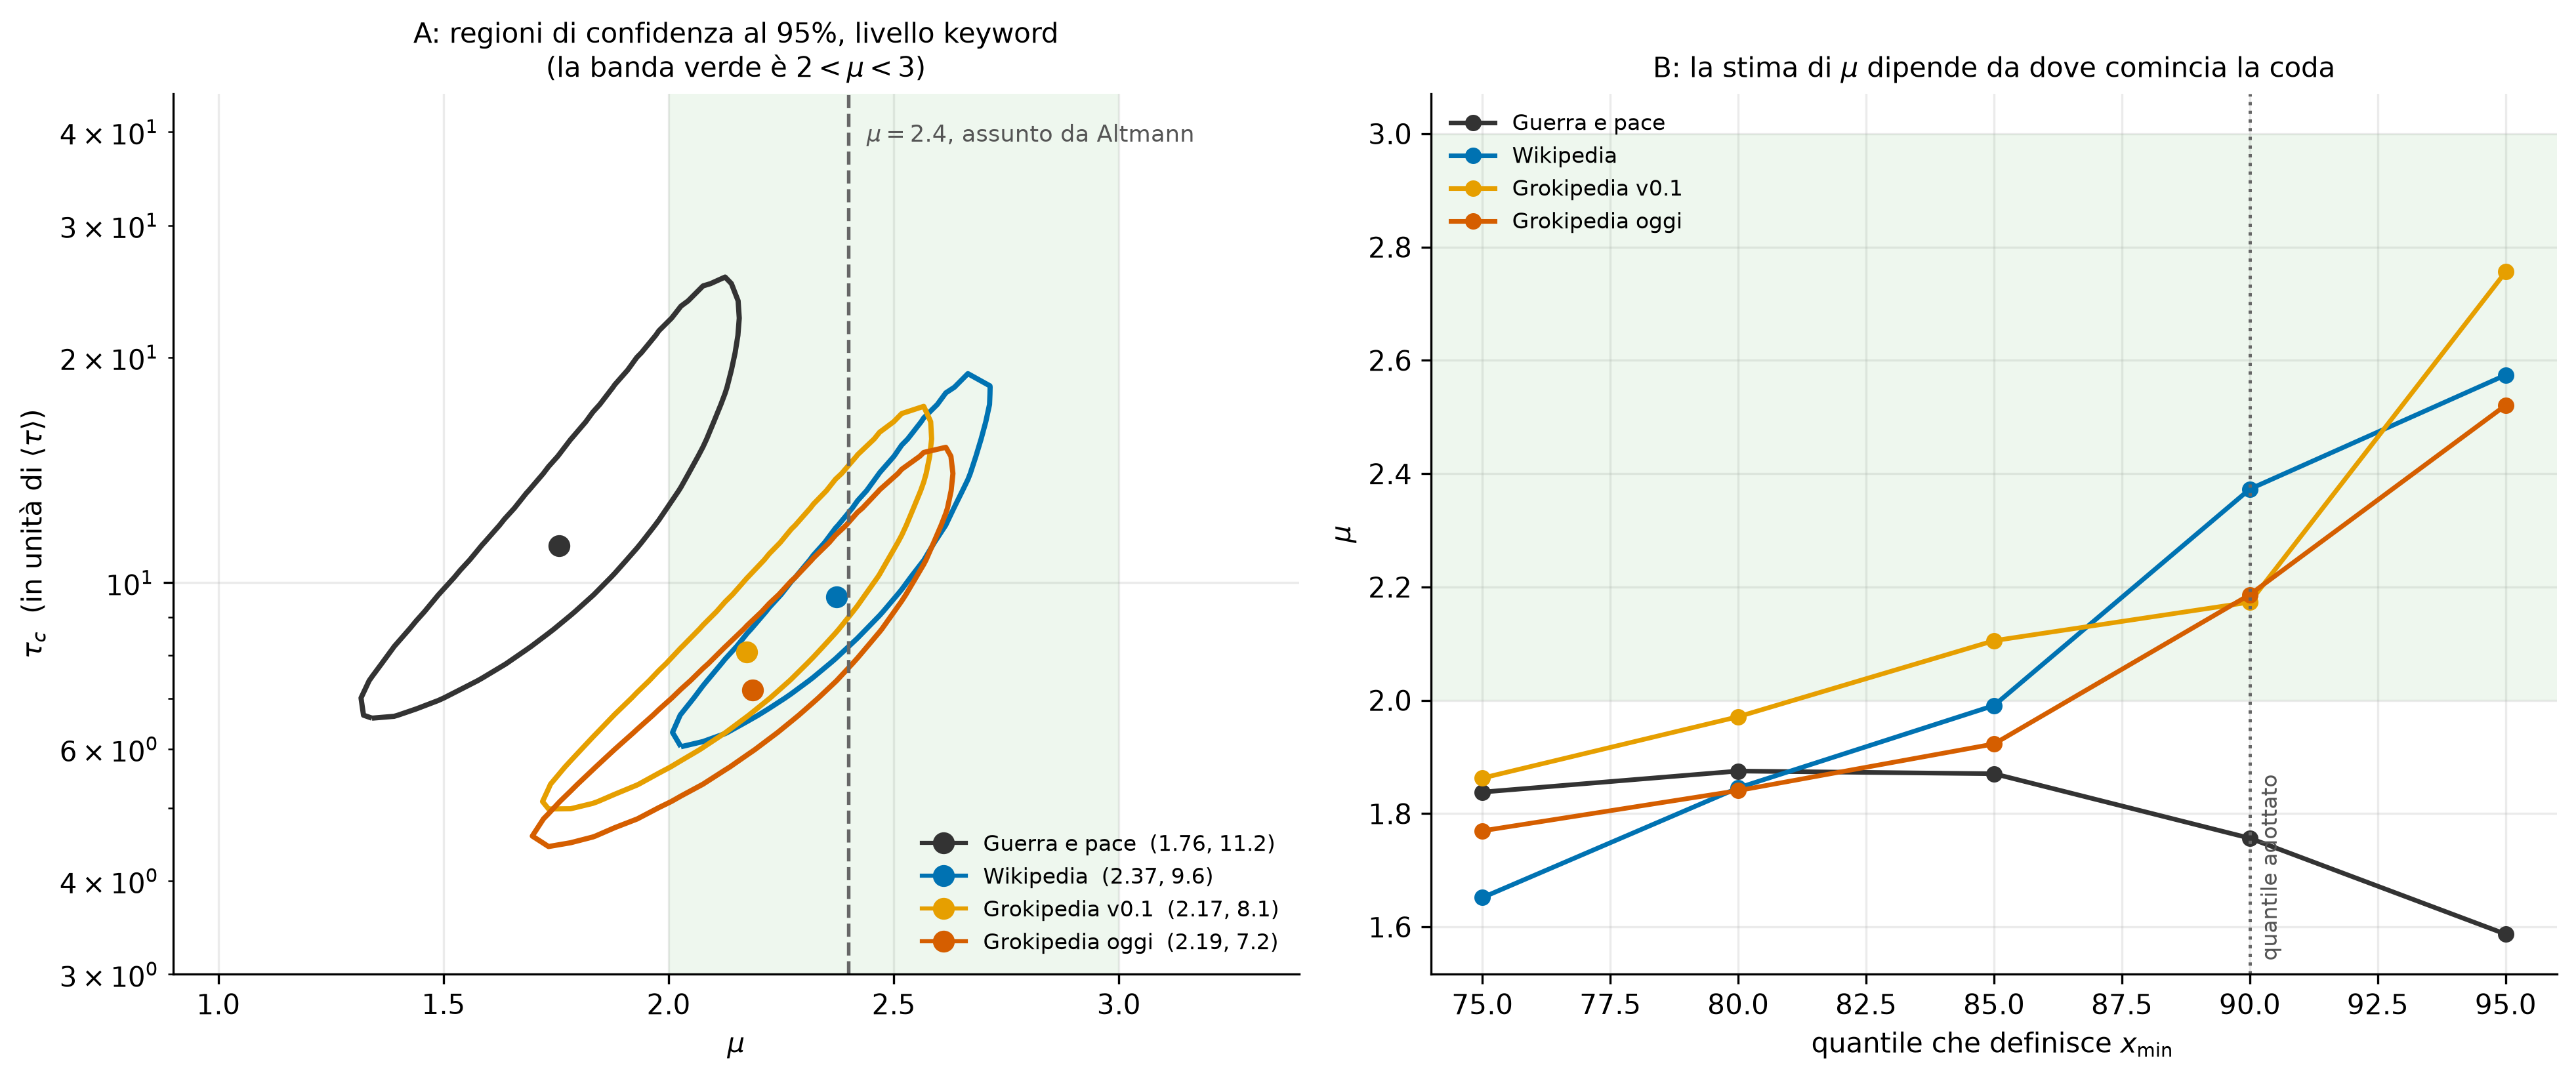
\includegraphics[width=\textwidth]{figure/cap5_verosimiglianza_coda.png}
  \caption{Perché l'esponente di coda non discrimina fra i corpora. A: regioni
  di confidenza congiunte al $95\%$ nel piano $(\mu, \tau_c)$ sul livello delle
  parole chiave, con $x_{\min}$ al novantesimo percentile; l'allungamento delle
  regioni è la correlazione fra i due parametri, e la linea tratteggiata è il
  valore $\mu = 2.4$ assunto in~\cite{altmann2012}. B: stima di $\mu$ al variare
  del quantile che definisce $x_{\min}$; le quattro curve si incrociano, cosicché
  l'ordinamento fra corpora dipende da quella scelta.}
  \label{fig:verosimiglianza}
\end{figure}

\paragraph{Il cut-off e la finestra di osservazione.} Il secondo pannello
della Figura~\ref{fig:coda} riporta $\tau_c$ ai quattro livelli, con
intervalli di confidenza di profilo. È l'altra metà di ciò
che~\cite{altmann2012} introduce senza stimare: il cut-off vi compare come
conseguenza necessaria della discesa nella gerarchia, ma non gli viene mai
assegnato un valore. Cresce in modo ordinato salendo nella gerarchia: circa
$1.1$ volte l'intervallo medio sulle lettere, dove la coda è di fatto già
esponenziale, $3.2$--$3.4$ sui controlli appaiati e $9.5$--$11.2$ sulle parole
chiave. La separazione fra i due livelli superiori è netta. Fra i quattro
corpora, invece, gli intervalli di confidenza si sovrappongono ampiamente:
neppure il cut-off ordina i corpora, e la sola cella in cui la separazione è
significativa è quella delle parole funzione del romanzo, discussa sopra.

Anche $\tau_c$ va poi letto come descrittore relativo alla lunghezza di analisi.
Ripetendo la stima sul romanzo a lunghezze crescenti, da \num{30000} a
\num{480000} caratteri, $\tau_c$ passa da $13.5$ a $94.7$: un fattore sette a
fronte di un fattore sedici sulla finestra, con un andamento non monotono che
scende prima di risalire. Il taglio non è dunque un puro artefatto, perché non
scala proporzionalmente alla finestra, ma non è nemmeno una lunghezza intrinseca
del testo. Sulla stessa serie $\mu$ si stabilizza attorno a $2.0$ alle finestre
maggiori, contro l'$1.76$ misurato alla lunghezza di lavoro: entrambi i
parametri descrivono la coda \emph{a quella lunghezza}, coerentemente con la
regola del §\ref{sec:lunghezza}.

\paragraph{Lo stimatore di Hill.} Dà sistematicamente valori più alti, $2.49$ sul
romanzo contro $1.76$ e circa $3.0$ sugli altri tre corpora contro
$2.2$--$2.4$, perché assume una legge di potenza pura su tutta la coda.
L'assenza di un plateau nel suo grafico diagnostico è ciò che ha motivato
l'adozione del modello troncato, e i suoi valori sono riportati solo a quel
titolo.

% ---------------------------------------------------------------------
\section{Entropia degli intervalli}
\label{sec:entropia-intervalli}

L'effetto di scala dichiarato nel §\ref{sec:appaiato} richiede una misura che
non risenta della lunghezza media delle frasi. È la ragione per cui il
§\ref{sec:entropia-intervalli-def} ha introdotto l'entropia degli intervalli
$J$ della~\eqref{eq:entropia-intervalli}: il logaritmo la rende invariante per
dilatazione dell'asse, cosicché frasi mediamente più lunghe non la spostano, e
la sottrazione del termine poissoniano ne cancella il bias. La grandezza è
risultata calcolabile su \num{5343} sequenze su \num{5617}, il $95\%$ del
totale.

\paragraph{Perché la misura è legittima.}
Trattandosi di una grandezza introdotta qui, la sua adozione va giustificata su
quello che fa e non su un precedente. I due ingredienti sono però entrambi
standard: l'entropia differenziale stimata per spaziature d'ordine è lo
stimatore di~\cite{vasicek1976}, e il confronto di una statistica osservata con
il valore che essa assume su un processo di Poisson di pari intensità è la
costruzione con cui in letteratura si misura la regolarità di una sequenza di
eventi, la stessa su cui poggiano la~\eqref{eq:cv} e il coefficiente
di~\cite{goh2008} usati nel resto del capitolo. Ciò che $J$ aggiunge è
l'invarianza per dilatazione, che nessuna delle due possiede e che serve qui per
una ragione specifica. Il §\ref{sec:entropia-intervalli-def} argomenta perché
debba funzionare; la validazione empirica è alla fine di questa sezione, dove la
stessa parola misurata a lunghezze diverse sposta il coefficiente di variazione
di un fattore tre e $J$ di due decimi di bit.

\paragraph{Che cosa riportano i tre pannelli.}
Il primo pannello della Figura~\ref{fig:entropia} mostra il rapporto fra $J$ e
il coefficiente di variazione sulle parole chiave. Le due misure sono
correlate, come atteso, ma la relazione non è biunivoca: a parità di
coefficiente di variazione i punti dei diversi corpora occupano fasce di $J$
diverse, il che è precisamente ciò che rende utile la seconda misura.

Il secondo pannello riporta $J$ ai quattro livelli. Sulle lettere i quattro
corpora coincidono attorno a $-0.20$, e sulle parole funzione i tre corpora
enciclopedici scendono insieme attorno a $-0.29$, con il romanzo che resta a
$-0.19$: valori negativi indicano intervalli più regolari di un
processo di Poisson. Sui due livelli superiori i corpora si separano, e sulle
parole chiave i corpora umani stanno sopra il valore poissoniano e quelli
generati vi si appoggiano: $J$ vale $+0.061$ sul romanzo e $+0.092$ su
Wikipedia, contro $-0.001$ su Grokipedia v0.1 e $-0.011$ sulla versione
attuale, questi ultimi due indistinguibili da zero. Le due enciclopedie generate
si collocano dunque sul valore poissoniano, mentre quella umana ne sta sopra:
gli intervalli fra parole chiave di Grokipedia non sono più regolari del caso,
semplicemente non sono più \emph{bursty} di esso. Il terzo pannello riporta la
distribuzione per documento e mostra che la separazione, pur con code
sovrapposte, riguarda l'intero corpus e non alcune voci.

\paragraph{La coda inferiore è fatta di soggetti di voce.}
La coda inferiore di quel pannello merita però un controllo, perché il cambio
di segno è ciò su cui l'affermazione precedente poggia. Le sequenze con $J$
più basso sono parole chiave a pieno titolo, nomi propri e non lessico di
servizio sfuggito alla lista chiusa, ma sono quasi tutte la stessa cosa: il
soggetto della voce. Fra le venti sequenze di $J$ minore, in Grokipedia
quattordici sono il soggetto dell'articolo, e in Wikipedia diciotto:
\emph{churchill}, \emph{newton}, \emph{paris}, \emph{freud}, \emph{mandela}. È
il fenomeno del §\ref{sec:tre-corpora}, che $J$ registra come gli altri
indicatori, e non è un difetto della classificazione.

Ha però una conseguenza sul cambio di segno. Escludendo i soggetti delle voci,
$54$ sequenze su $273$ in Grokipedia e $57$ in Wikipedia, tutti e tre i
corpora enciclopedici passano sopra il valore poissoniano: $+0.175$ su
Wikipedia e $+0.070$ su Grokipedia. Il divario appaiato sopravvive, $-0.087$
bit con $p < 10^{-3}$, e con esso la conclusione del paragrafo; non sopravvive
invece la lettura per segno, perché il segno negativo di Grokipedia è prodotto
dai soggetti delle voci, che il §\ref{sec:tre-corpora} ha già mostrato essere
marcatori sintattici e non semantici. Ciò che distingue i due corpora è quanto
$J$ vale, non da che parte dello zero cade.

\paragraph{Il divario appaiato.}
I confronti appaiati confermano il divario: sulle parole chiave la differenza
mediana fra Grokipedia attuale e Wikipedia vale $-0.105$ bit e quella fra la
v0.1 e Wikipedia $-0.077$ bit, entrambe con significatività inferiore a
$10^{-3}$. Sulle lettere e sulle parole funzione, per contro, le differenze sono
positive e non significative. Poiché $J$ non risente della diversa lunghezza
delle frasi, questo risultato conferma il divario del §\ref{sec:appaiato}
senza risentire di quell'effetto, ed è il punto in cui la conclusione principale
del capitolo diventa difendibile.

\paragraph{Perché il divario è più ampio sui controlli.}
Il divario è però più ampio sui controlli appaiati, $-0.209$ bit, che sulle
parole chiave, e la ragione sta in che cosa siano quei controlli. Il controllo
di una parola chiave è la parola di frequenza più vicina fra quelle che restano
dopo aver tolto le parole chiave stesse, i nomi propri e le sei parole funzione
selezionate; poiché le parole chiave sono per costruzione le più frequenti del
loro tipo, ciò che resta a quelle frequenze è in larga parte lessico di
servizio. I controlli più ricorrenti sono infatti \emph{by}, \emph{from},
\emph{with} e \emph{as} in Wikipedia, e \emph{like}, \emph{but}, \emph{that} e
\emph{this} in Grokipedia. È il livello in cui il testo generato si distingue di
più: le sue parole di servizio sono distribuite quasi uniformemente,
$J = -0.165$, mentre quelle di Wikipedia conservano un residuo di
addensamento, $J = +0.053$.

\paragraph{Composizione e stile, in parti quasi uguali.}
Le due liste di controlli sono però diverse fra loro, e la differenza potrebbe
misurare quali parole vengono selezionate anziché come sono distribuite. Le due
cause si separano restringendo il confronto alle parole che compaiono fra i
controlli di entrambi i corpora. Sono ventisei, e dodici raggiungono almeno tre
voci per corpus. Su queste il divario resta: la differenza mediana di $J$ vale
$-0.091$ bit con $p = 0.043$, e le quattro parole più spostate sono
\emph{with} ($-0.060$ contro $-0.414$), \emph{as} ($+0.227$ contro $-0.106$),
\emph{this} ($-0.005$ contro $-0.301$) e \emph{from} ($+0.057$ contro $-0.225$).
Il divario fra le medie dei due corpora, $-0.218$ bit, si scompone dunque in
$-0.128$ attribuibili alla distribuzione delle stesse parole e $-0.091$ alla
diversa composizione delle due liste, cioè in parti quasi uguali. Il valore
differisce di un centesimo dal $-0.209$ citato sopra perché quello è la mediana
delle differenze voce per voce e questo la differenza fra le medie.

La parte attribuibile alla composizione ha un contenuto proprio. I controlli di
Wikipedia sono preposizioni e ausiliari legati alla struttura del periodo, come
\emph{by}, \emph{was}, \emph{with} e \emph{for}; quelli di Grokipedia sono in
prevalenza connettivi di discorso, come \emph{like}, \emph{but}, \emph{that} e
\emph{over}. La parte attribuibile alla distribuzione descrive invece un
meccanismo: in Wikipedia una preposizione come \emph{from} si addensa dove il
contenuto la richiede, in una sezione biografica più che in una tecnica, e i suoi
intervalli ereditano il ritmo delle sezioni; in Grokipedia la stessa parola
ricorre a cadenza quasi costante lungo tutto l'articolo. Il segno negativo di $J$
dice che quella cadenza è più regolare di quella di un processo casuale, non
soltanto meno addensata.

Una verifica interna conferma la lettura. Nei controlli di Wikipedia il $93\%$
delle parole appartiene alla lista chiusa e dà $J = +0.043$, mentre il restante
$7\%$ dà $+0.188$: la classe grammaticale della parola cambia il risultato. In
Grokipedia le due quote valgono $-0.151$ e $-0.182$, indistinguibili fra loro.
Nel testo generato la regolarità degli intervalli non dipende da che tipo di
parola si stia guardando, ed è la stessa compressione uniforme della variabilità
lessicale che il §\ref{sec:sintesi-cap5} indica come conclusione del capitolo,
osservata al livello in cui si manifesta con più forza.

\paragraph{Stabilità rispetto alla lunghezza di analisi.}
Una validazione indipendente riguarda la dipendenza dalla lunghezza. Passando
da \num{40000} caratteri al romanzo intero, il coefficiente di variazione della
parola \emph{prince} cambia di un fattore $3.08$, mentre il suo $J$ si sposta di
$0.21$ bit; per la parola \emph{pierre} il coefficiente cambia di un fattore
$3.49$ e $J$ di $0.08$ bit. I due numeri non sono direttamente confrontabili,
perché il coefficiente di variazione è un rapporto e $J$ un logaritmo: uno
spostamento di $0.21$ bit corrisponde a un fattore $2^{0.21} = 1.16$ sulla
dispersione efficace degli intervalli, e uno di $0.08$ bit a un fattore $1.06$.
Riportate alla stessa scala, le due derive stanno nel rapporto di $2.7$ e $3.3$
in favore di $J$. La nuova misura è dunque circa tre volte più stabile rispetto
alla lunghezza di analisi di quella che sostituisce, il che ne conferma
l'utilità al di là del problema specifico per cui era stata introdotta.

\begin{figure}[htbp]
  \centering
  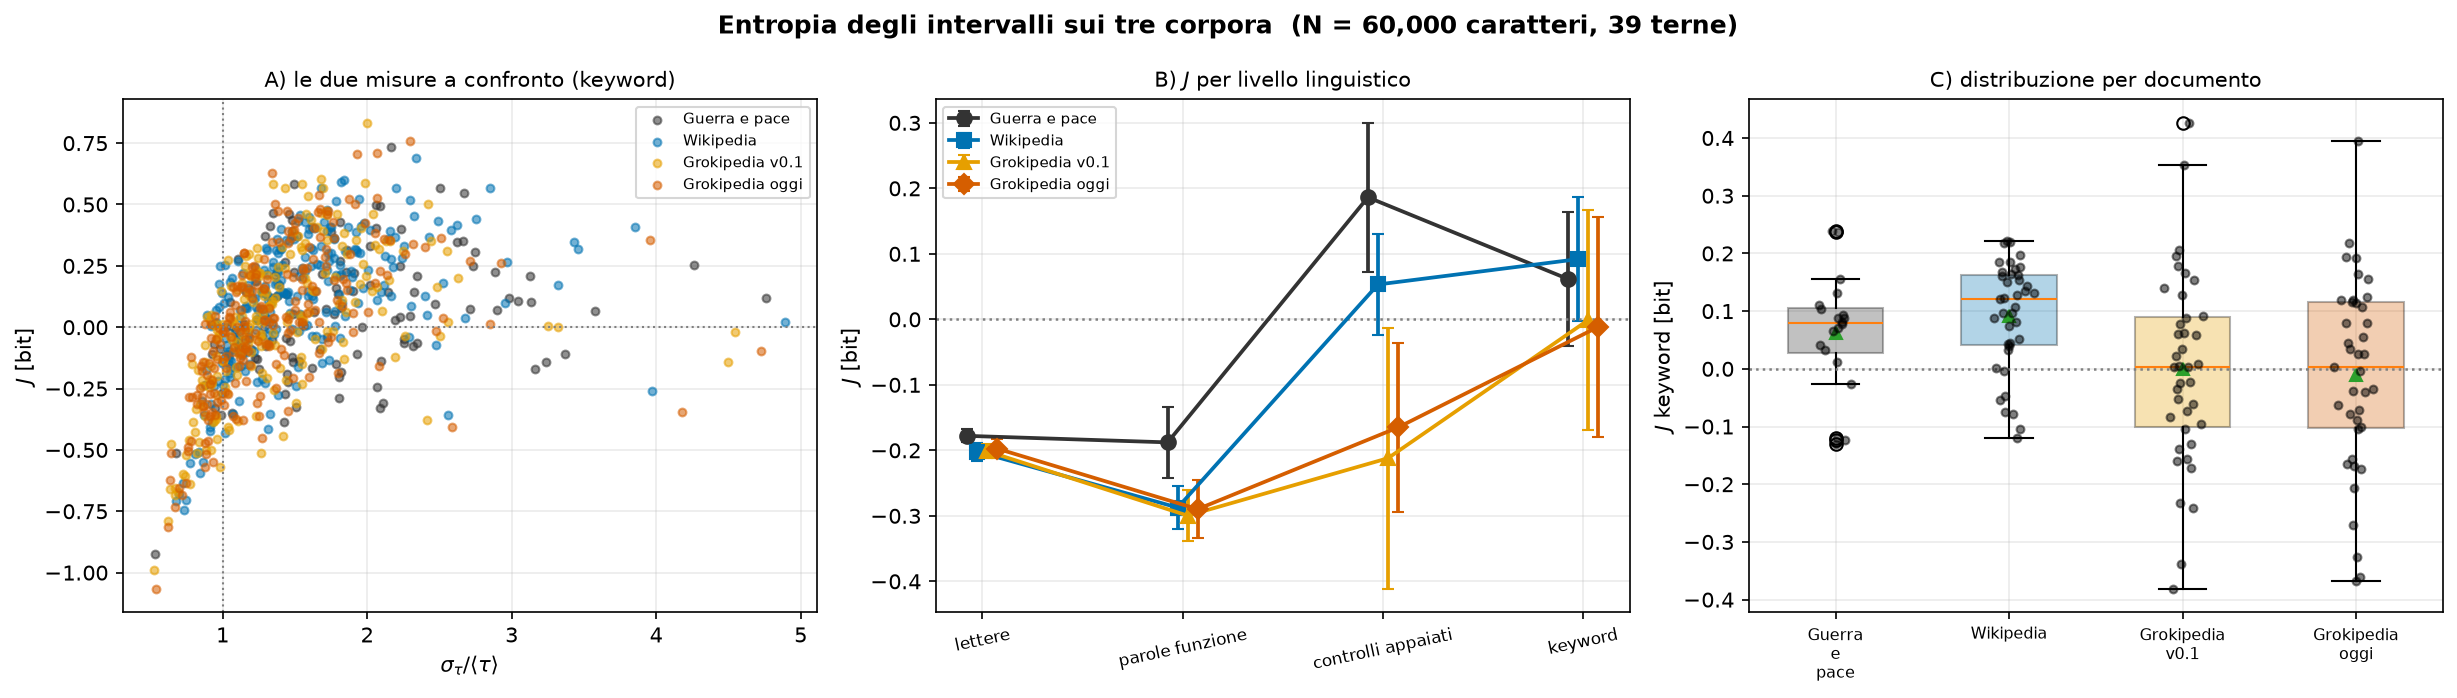
\includegraphics[width=\textwidth]{figure/cap5_entropia_intervalli.png}
  \caption{Entropia degli intervalli. A: relazione fra $J$ e coefficiente di
  variazione sulle parole chiave, un punto per sequenza. B: $J$ ai quattro
  livelli linguistici, con deviazioni standard fra testi; valori negativi
  indicano intervalli più regolari di un processo di Poisson. C: distribuzione
  di $J$ sulle parole chiave documento per documento. La misura è invariante per
  dilatazione dell'asse dei caratteri e non risente quindi della diversa
  lunghezza delle frasi nei due corpora enciclopedici.}
  \label{fig:entropia}
\end{figure}

% ---------------------------------------------------------------------
\section{Quanto pesa la definizione dei livelli lessicali}
\label{sec:effetto-stoplist}

Il paragrafo \emph{Come vengono separati i livelli lessicali} del
§\ref{sec:scelte} ha documentato l'estensione della lista chiusa di parole funzione da
\num{133} a \num{215} voci e la ragione per cui era necessaria. Questa sezione
riporta di quanto si spostano i risultati, perché lo spostamento non è
trascurabile e la scelta deve restare verificabile.

Il pannello A della Figura~\ref{fig:effetto-stoplist} riporta quali parole la
lista originaria lasciava passare fra le parole chiave di Grokipedia, e in
quante voci ciascuna: nell'elenco corrispondente di Wikipedia non ne compare
nessuna, e le sue sette parole sono distinte fra loro, ciascuna in una sola
voce.

\begin{table}[htbp]
  \centering
  \begin{tabular}{lcccc}
    \toprule
    & \multicolumn{2}{c}{lista originaria} & \multicolumn{2}{c}{lista estesa} \\
    \cmidrule(lr){2-3}\cmidrule(lr){4-5}
    & Wikipedia & Grok. oggi & Wikipedia & Grok. oggi \\
    \midrule
    keyword più bursty del controllo & $0.685$ & $0.630$ & $0.692$ & $0.740$ \\
    idem, su $\hat\gamma$ & $0.736$ & $0.663$ & $0.747$ & $0.791$ \\
    $\sigma_\tau/\langle\tau\rangle$ keyword & $1.530$ & $1.289$ & $1.536$ & $1.379$ \\
    divario appaiato, keyword & \multicolumn{2}{c}{$-0.230$} & \multicolumn{2}{c}{$-0.167$} \\
    divario appaiato, controlli & \multicolumn{2}{c}{$-0.122$} & \multicolumn{2}{c}{$-0.157$} \\
    $J$ keyword & $+0.086$ & $-0.069$ & $+0.092$ & $-0.011$ \\
    $\mu$ keyword & $2.38$ & $2.52$ & $2.37$ & $2.19$ \\
    quadrante basso-sinistra & $5.1\%$ & $24.5\%$ & $5.1\%$ & $14.3\%$ \\
    \bottomrule
  \end{tabular}
  \caption{Effetto della definizione dei livelli lessicali sui risultati del
  capitolo. Le righe dei divari appaiati riportano un solo valore perché
  misurano la differenza fra i due corpora. Le lettere e le parole funzione non
  compaiono perché nessuna parola cambia livello a quelle altezze: i loro valori
  coincidono a tutte le cifre riportate nel capitolo.}
  \label{tab:effetto-stoplist}
\end{table}

La Tabella~\ref{tab:effetto-stoplist} riporta il confronto. Tre risultati
cambiano in modo sostanziale. Il primo è il test interno: con la lista
originaria Grokipedia sembrava battere il proprio controllo appaiato meno spesso
di Wikipedia, e l'ordinamento fra i corpora appariva netto; con la lista estesa
l'ordine si inverte, e la differenza fra le due enciclopedie sparisce. Il
pannello B della figura mostra i due esiti sovrapposti. Il secondo è l'entropia
degli intervalli, il cui valore sulle parole chiave passa da $-0.069$ a
$-0.011$, cioè da un cambio di segno netto a uno indistinguibile da zero. Il
terzo è l'esponente di coda, che su Grokipedia scende da $2.52$ a $2.19$,
avvicinandosi a quello di Wikipedia anziché allontanarsene.

Restano invece stabili il divario appaiato complessivo, che si riduce da
$-0.230$ a $-0.167$ senza perdere significatività, il coefficiente di variazione
delle parole chiave, e l'intera decomposizione della~\eqref{eq:eq4}. Non si
muovono di una cifra, come è ovvio, i livelli delle lettere e delle parole
funzione.

La lezione metodologica vale al di là di questo caso. La distinzione fra
parole di contenuto e parole di servizio è la premessa dell'intero protocollo
di~\cite{altmann2012}, e viene qui operata da una lista chiusa che il paper
non specifica. Quando i corpora confrontati hanno abitudini lessicali diverse,
e un modello linguistico ne ha rispetto a un redattore umano, una lista
incompleta non introduce un rumore simmetrico: sposta sistematicamente in un
solo corpus il confine fra i due livelli, e produce un divario che non c'è.

\begin{figure}[htbp]
  \centering
  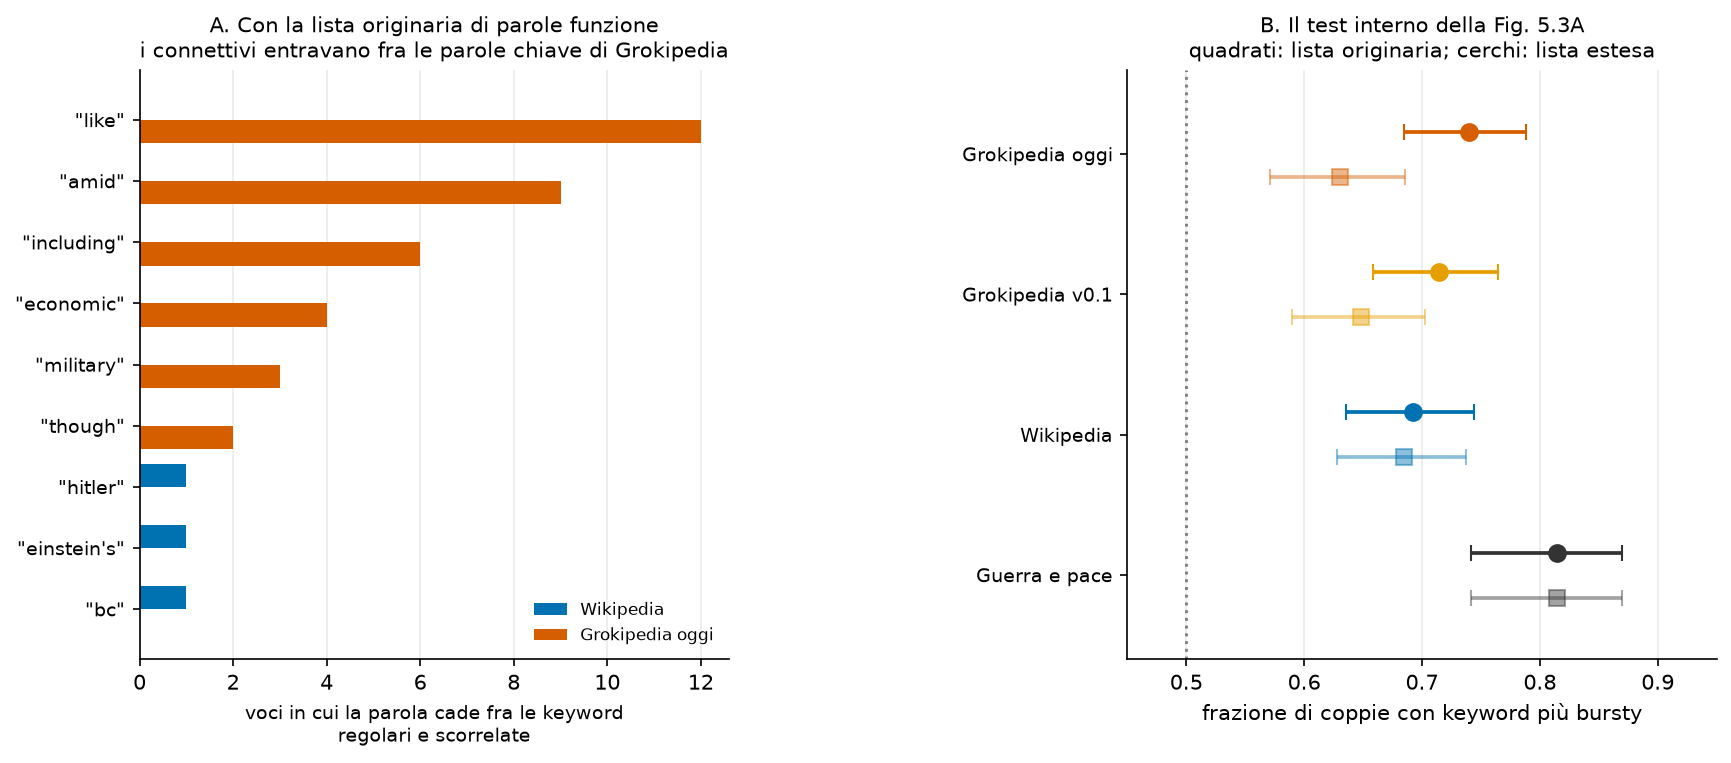
\includegraphics[width=\textwidth]{figure/cap5_effetto_stoplist.png}
  \caption{Effetto della definizione dei livelli lessicali. A: con la lista di
  funtori originaria, quali parole cadevano fra le parole chiave classificate
  come regolari e scorrelate, contate come numero di voci in cui ciò accadeva;
  le prime tre di Grokipedia sono connettivi, e in Wikipedia non compaiono. B:
  il test interno della Figura~\ref{fig:tre-corpora}A con le due
  classificazioni, quadrati per la lista originaria e cerchi per quella estesa,
  con intervalli di confidenza al $95\%$.}
  \label{fig:effetto-stoplist}
\end{figure}

% ---------------------------------------------------------------------
\section{Che cosa il testo generato non riproduce}
\label{sec:sintesi-cap5}

Il testo generato possiede correlazioni a lungo raggio, e ai livelli bassi della
gerarchia linguistica le possiede quasi nella stessa misura del testo umano:
sulle lettere i quattro corpora sono indistinguibili per coefficiente di
variazione, per entropia degli intervalli e per quota di burstiness, e sulle
parole funzione la differenza è piccola, benché significativa. Al livello delle parole il divario si apre, e vale più di un ordine
di grandezza rispetto a quello misurato sui caratteri.

Il divario non distingue però le parole che portano il contenuto dai controlli a
frequenza appaiata. I due valori sono quasi uguali alla lunghezza di lavoro,
$-0.157$ e $-0.167$, e si invertono a quella di controllo
(§\ref{sec:robustezza-neff}); e il test che chiede se la parola chiave superi il
proprio controllo \emph{dentro lo stesso testo} dà a Grokipedia un esito pari a
quello di Wikipedia, anzi lievemente migliore. Il meccanismo descritto
in~\cite{altmann2012} è dunque presente nel testo generato, e con la stessa
efficacia: ciò che manca è l'ampiezza con cui le parole, di contenuto e non, si
addensano.

Non si tratta dunque di una persistenza tematica assente, perché la distinzione
fra parole tematiche e parole ordinarie il modello la produce; si tratta di una
compressione uniforme della variabilità lessicale, che riduce la burstiness di
tutte le parole senza alterare il rapporto fra le une e le altre. Vale ancora la
distinzione posta nel §\ref{sec:intro-linguaggio} fra riprodurre le proprietà
statistiche del linguaggio e riprodurre il meccanismo che le genera, ma
applicata a un livello più basso di quanto la prima lettura suggerisse.

Ciò che il capitolo misura è la distanza fra due enciclopedie appaiate titolo
per titolo, e null'altro. Il deficit è osservato su Grokipedia, cioè su un unico
sistema generativo, in un unico dominio e in una sola lingua: nulla di quanto
riportato qui stabilisce che sia una proprietà dei modelli linguistici in
generale anziché di quel sistema. Il Capitolo~\ref{cap:risultati1} non offre un
appoggio indipendente su questo punto: misura un altro corpus, con grandezze
che non arrivano al livello a cui il divario si manifesta.

%
%  Tre lunghezze di analisi con corpora diversi, da non confondere:
%    fattibilità  50 000 caratteri, 40 voci  (§5.2)
%    analisi      60 000 caratteri, 39 terne (§5.3--5.7)
%    robustezza   80 000 caratteri, 35 terne (§5.8)
% =====================================================================

\chapter{Burstiness lessicale in corpora umani e generativi}
\label{cap:risultati2}

% ---------------------------------------------------------------------
\section{Perché un secondo corpus}
\label{sec:perche-wiki}

Questo capitolo nasce da un esito negativo del precedente. Il
§\ref{sec:fallimenti} ha mostrato che dei \num{242} documenti generati lungo lo
sweep soltanto due non ricadono in alcuna modalità di degenerazione, ed entrambi
si trovano a $T = 1.0$. Il protocollo introdotto nel §\ref{sec:burst} è però un
protocollo semantico: richiede di individuare in ciascun testo le parole che ne
portano il contenuto e di misurare come si distribuiscono le distanze fra le
loro occorrenze successive. Su un testo che ripete lo stesso ciclo di parole, o
su una sequenza degenerata nel senso opposto, 
quelle distanze si calcolano ancora ma non misurano più la
persistenza di un tema. Applicare il protocollo al corpus dello sweep
restituirebbe numeri privi di contenuto.

Il confronto viene quindi spostato su un dominio in cui la qualità del testo
non è una variabile. Wikipedia e Grokipedia trattano le stesse voci, la prima
scritta da esseri umani e la seconda generata da un modello linguistico, ed
entrambe producono prosa espositiva ben formata. Appaiare le due enciclopedie
per titolo tiene inoltre fisso l'argomento trattato: la voce
\emph{Albert Einstein} di Wikipedia e quella di Grokipedia parlano della stessa
cosa, e qualunque differenza nella statistica degli intervalli non può essere
attribuita a un argomento diverso. I corpora sono descritti nel §\ref{sec:corpora}, e le
due versioni di Grokipedia nel §\ref{sec:paternita}.

Il romanzo di riferimento resta nell'analisi come ancora letteraria: è il
dominio su cui il protocollo è stato formulato, e serve a dire quanto la prosa
enciclopedica si discosti già di per sé dal caso studiato in origine.

% ---------------------------------------------------------------------
\section{Il protocollo regge sulla prosa enciclopedica}
\label{sec:fattibilita}

Prima di confrontare due enciclopedie occorre stabilire che l'effetto da
confrontare esista nella prima. Il protocollo di Altmann è stato costruito e
validato su romanzi, e la prosa enciclopedica ha una struttura diversa: non ha
trama, procede per sezioni tematiche dichiarate da titoli, e la persistenza di
un argomento vi si manifesta in modo più rigido. Che le parole di contenuto vi
risultino più \emph{bursty} dei propri controlli non è quindi scontato.

La verifica è stata condotta su \num{40} voci di Wikipedia troncate a
\num{50000} caratteri, contro \num{20} segmenti del romanzo della stessa
lunghezza: è la fase di fattibilità della Tabella~\ref{tab:fasi}, l'unica del
capitolo a impiegare quella lunghezza e quel numero di voci, e i suoi
denominatori non vanno confusi con quelli delle sezioni successive. La
Figura~\ref{fig:wiki-fattibilita} ne riporta l'esito. Il primo
pannello confronta ciascuna parola chiave con il proprio controllo appaiato in
frequenza e riporta la quota di confronti vinti dalla parola chiave: il valore
$0.5$ corrisponde all'assenza di effetto. Su Wikipedia la quota vale
$197/280 = 0.704$ per il coefficiente di variazione e $216/280 = 0.771$ per
l'esponente di correlazione, con estremi inferiori degli intervalli di
confidenza pari a $0.65$ e $0.72$: l'effetto esiste. Sul romanzo le stesse
quote valgono $104/140 = 0.743$ e $123/140 = 0.879$, cioè sono più alte, ma la
differenza non annulla il segnale enciclopedico.

Il secondo pannello mostra da dove viene quel segnale, ed è utile precisare
come i suoi valori siano costruiti, perché la stessa procedura vale per tutte
le figure per livello del capitolo. Dentro ciascun testo si selezionano più
sequenze per livello: diciannove lettere, sei parole funzione, sette parole
chiave e i sette controlli appaiati. Per ognuna si misura
$\sigma_\tau/\langle\tau\rangle$ sui suoi intervalli. I valori delle sequenze
dello stesso livello si mediano poi dentro il testo, ottenendo un
numero per coppia (testo, livello); infine si media su tutti i testi del
corpus, ed è questo secondo valore a comparire nel pannello, con la barra
d'errore data dalla deviazione standard fra testi. Con questa costruzione il
coefficiente di variazione $CV$ cresce salendo lungo i quattro livelli in entrambi
i corpora e con lo stesso andamento: le lettere stanno sotto l'unità, cioè si
distribuiscono in modo più regolare di un processo di Poisson, mentre le
parole chiave arrivano a $1.51$ su Wikipedia e a $1.62$ sul romanzo. Il terzo
pannello riporta la distribuzione dei singoli testi attorno a quelle medie e
mostra che la sovrapposizione fra i due corpora è ampia, con mediane vicine e
code che si intersecano.

Il rapporto fra le due burstiness delle parole chiave vale $0.93$: la prosa
enciclopedica è meno \emph{bursty} del romanzo, ma dello stesso ordine. Il protocollo
regge, e il confronto con Grokipedia ha un segnale da rilevare.

\begin{figure}[htbp]
  \centering
  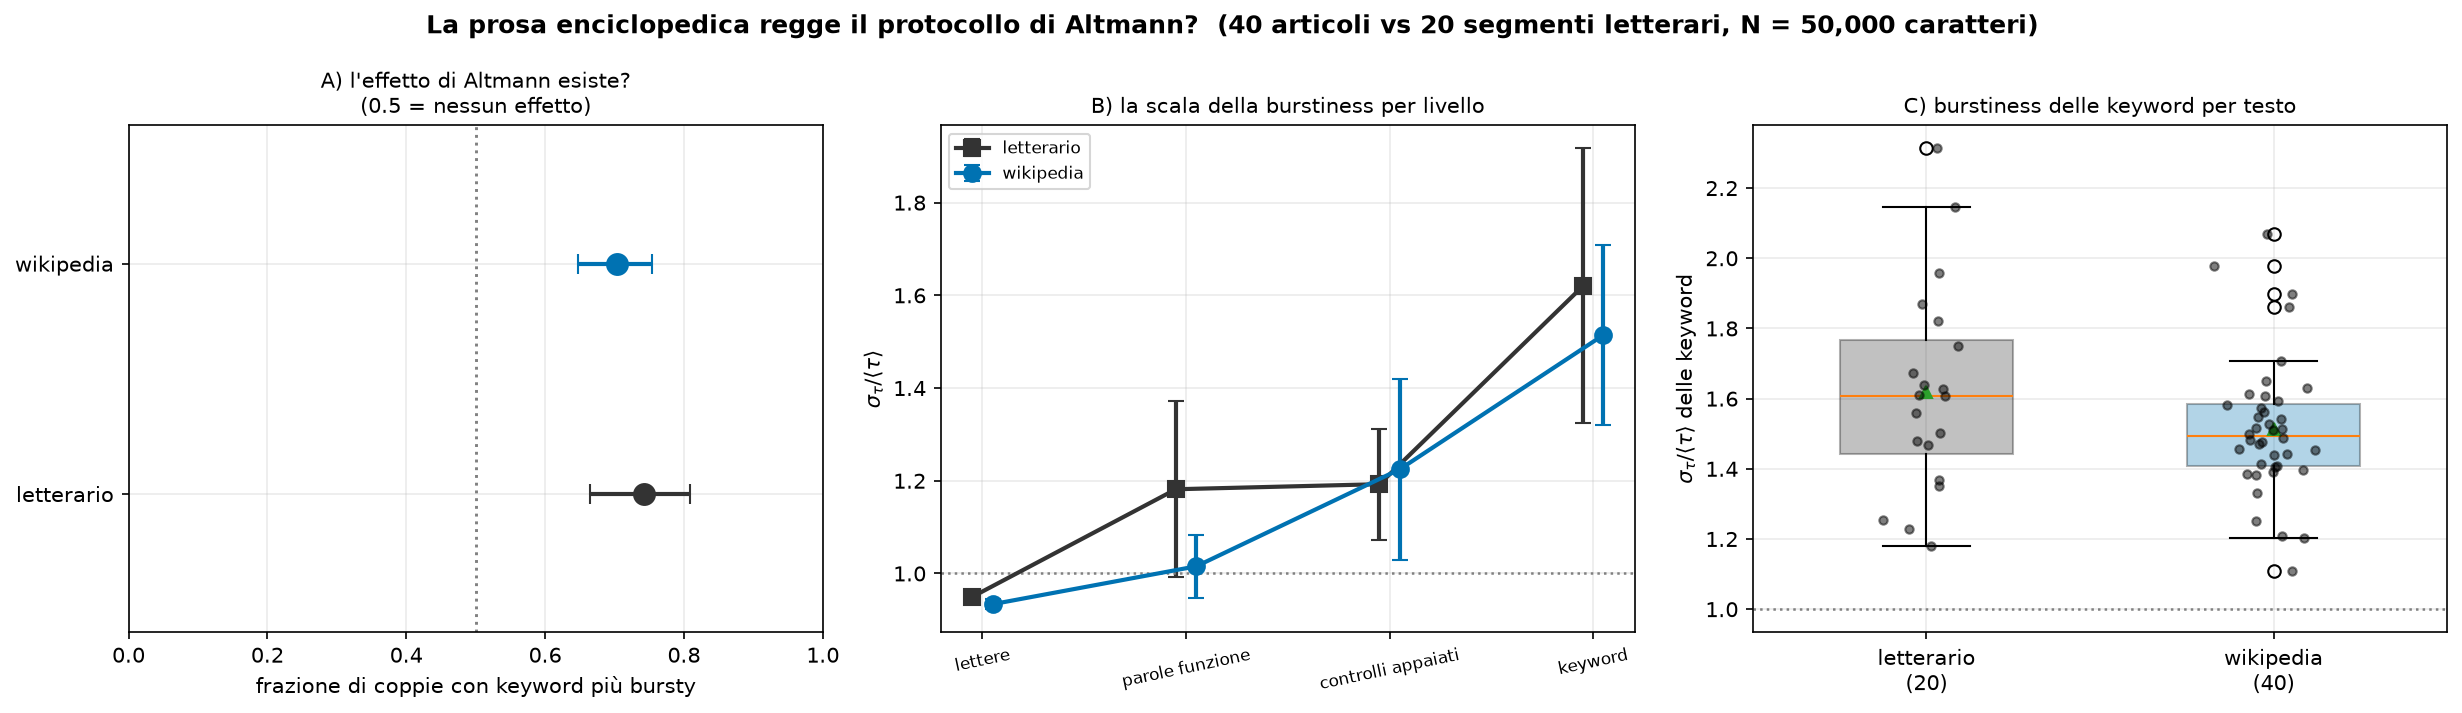
\includegraphics[width=\textwidth]{figure/cap5_wiki_altmann.png}
  \caption{Test di fattibilità del protocollo su prosa enciclopedica, condotto
  su \num{40} voci di Wikipedia e \num{20} segmenti letterari a \num{50000}
  caratteri. A: quota di confronti in cui la parola chiave supera il proprio
  controllo appaiato in frequenza, con intervallo di confidenza al $95\%$; la
  linea punteggiata a $0.5$ è l'assenza di effetto. B: coefficiente di
  variazione degli intervalli ai quattro livelli linguistici. C: distribuzione
  della burstiness delle parole chiave testo per testo. Questa è l'unica figura
  del capitolo costruita su \num{40} voci e \num{50000} caratteri; tutte le
  successive usano \num{39} terne e \num{60000} caratteri.}
  \label{fig:wiki-fattibilita}
\end{figure}

% ---------------------------------------------------------------------
\section{L'effetto nei tre corpora}
\label{sec:tre-corpora}

L'analisi principale confronta Wikipedia, le due versioni di Grokipedia e
l'ancora letteraria su \num{39} terne complete, troncate a \num{60000}
caratteri. La voce esclusa è \emph{Buddhism}, per la ragione riportata nel
§\ref{sec:paternita}: la sua versione v0.1 è ricopiata da Wikipedia, e in un
disegno appaiato un titolo che cade in un corpus deve cadere in tutti.

\paragraph{La finestra su cui l'esponente è stimato.}
L'esponente di correlazione $\hat\gamma$ è ottenuto interpolando
la~\eqref{eq:sigma} nell'intervallo fisso $t \in (100, 2000)$ caratteri.
\cite{altmann2012} adotta invece una regola relativa e ferma la finestra
all'uno per cento della lunghezza del testo. Le due scelte non sono ordinabili
una volta per tutte: applicata ai romanzi interi che quel lavoro analizza la
regola relativa dà un tetto dell'ordine di \num{10000} caratteri, molto più
largo di quello adottato qui; applicata alle finestre da \num{60000} caratteri
di questo capitolo dà $t < 600$, molto più stretto. L'intera catena è stata
ripetuta anche con la seconda. Il
livello medio di $\hat\gamma$ si abbassa di qualche centesimo, sulle parole
chiave da $1.23$ a $1.18$ per Wikipedia e da $1.32$ a $1.22$ per il romanzo,
ma l'ordinamento fra i corpora resta identico a tutti e quattro i livelli. Il
divario appaiato fra Grokipedia attuale e Wikipedia sulle parole chiave passa
da $-0.049$ a $-0.076$, cioè si accentua invece di ridursi, e resta
significativo in entrambi i casi. Le conclusioni di questo capitolo non
dipendono dunque dalla finestra scelta.

\paragraph{Tre modi di leggere il confronto.}
La Figura~\ref{fig:tre-corpora} riporta i tre modi in cui il confronto può
essere letto. Il primo pannello ripete il test del paragrafo precedente sui
quattro corpora: la quota di confronti vinti dalle parole chiave vale
$114/140 = 0.814$ sul romanzo, $189/273 = 0.692$ su Wikipedia,
$195/273 = 0.714$ su Grokipedia v0.1 e $202/273 = 0.740$ su Grokipedia nella
versione attuale. Ripetendo lo stesso test sull'esponente di correlazione
$\hat\gamma$ anziché sulla burstiness, la quota di confronti vinti dalle parole
chiave vale $0.907$ sul romanzo, $0.747$ su Wikipedia, $0.769$ su Grokipedia
v0.1 e $0.791$ su Grokipedia nella versione attuale.
L'effetto esiste ovunque, con tutti e quattro gli
intervalli di confidenza interamente sopra $0.5$, ed è massimo sul romanzo;
fra le due enciclopedie, però, non distingue: i valori di Grokipedia sono anzi
lievemente superiori a quelli di Wikipedia, con intervalli che si sovrappongono.
La domanda a cui questo pannello risponde è se la parola chiave superi il
proprio controllo a frequenza appaiata dentro lo stesso testo, e la
risposta è che ciò accade con la stessa frequenza nei due corpora enciclopedici.
Il deficit di Grokipedia, misurato dai pannelli successivi, non riguarda dunque
l'esistenza del meccanismo ma il livello assoluto della burstiness.

Il secondo pannello mostra il coefficiente di variazione ai quattro livelli e
rende visibile dove la differenza si concentra. Sulle lettere i quattro corpora
sono indistinguibili, tutti compresi fra $0.922$ e $0.950$, e sulle parole
funzione la separazione resta modesta, da $0.967$ a $1.192$. Il divario si apre
ai due livelli lessicali: sui controlli appaiati il romanzo raggiunge $1.262$,
Wikipedia $1.190$ e le due versioni di Grokipedia $1.044$ e $1.055$; sulle
parole chiave rispettivamente $1.789$, $1.536$, $1.387$ e $1.379$. 
Il terzo pannello riporta la stessa quantità testo per testo,
e mostra che la separazione non è l'effetto di pochi articoli anomali: le
distribuzioni di Wikipedia e di Grokipedia si sovrappongono, ma le loro mediane
differiscono di circa $0.25$ e la coda superiore di Wikipedia è più popolata.

\begin{figure}[htbp]
  \centering
  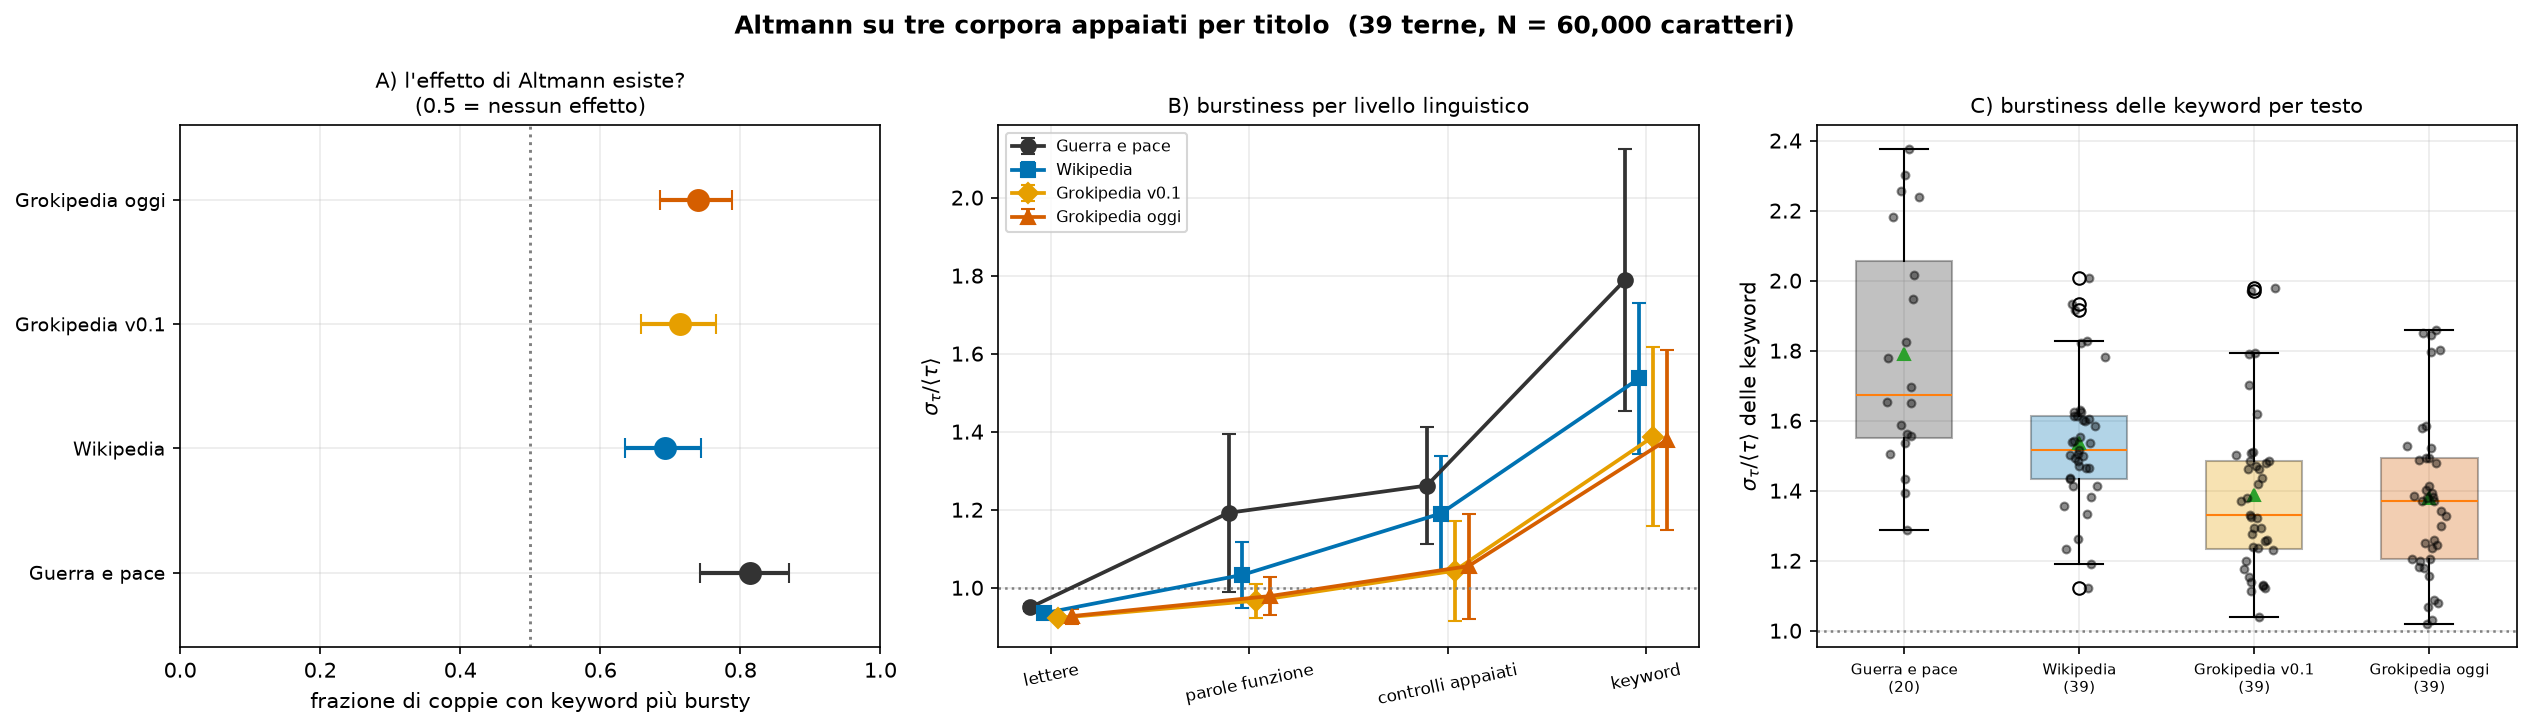
\includegraphics[width=\textwidth]{figure/cap5_tre_corpora.png}
  \caption{Il protocollo di Altmann sui quattro corpora, \num{39} terne
  appaiate per titolo a \num{60000} caratteri. A: quota di confronti vinti dalle
  parole chiave, con intervallo di confidenza al $95\%$. B: coefficiente di
  variazione degli intervalli ai quattro livelli linguistici; le barre sono
  deviazioni standard fra testi. C: burstiness delle parole chiave testo per
  testo, con mediana, quartili e singoli punti sovrapposti. Il numero di testi
  per corpus è indicato sotto ciascuna colonna.}
  \label{fig:tre-corpora}
\end{figure}

\paragraph{L'ancora letteraria è un testo, non un genere.} Il primato del
romanzo sui due livelli lessicali non sopravvive al cambio di testo. Ripetendo
l'intera misura su tre altri romanzi inglesi trattati esattamente come
\emph{Guerra e pace}, cioè \emph{Moby Dick}, \emph{Middlemarch} e \emph{David
Copperfield}, gli stessi impiegati come controllo nel
§\ref{sec:coda-risultati}, sulle parole chiave si ottiene $1.55$, $1.54$ e
$1.63$, cioè valori sostanzialmente pari a quello di Wikipedia e ben al di
sotto dell'$1.79$ di \emph{Guerra e pace}; alle parole funzione si ottiene
$1.03$, $1.08$ e $1.09$, contro l'$1.19$ del romanzo di riferimento e l'$1.03$
di Wikipedia. La distanza fra prosa letteraria e prosa enciclopedica non è
dunque un fatto generale, e l'ancora letteraria di questo capitolo va letta
per ciò che è: un termine di paragone concreto, non la misura di un genere.
Nulla di ciò che segue vi poggia, perché il risultato del capitolo è un
confronto appaiato fra le due enciclopedie, dove il romanzo non entra.

Il null model A1 restituisce un esponente medio di $0.983$ su tutte le celle,
in accordo con l'unità che deve dare per costruzione: la procedura di stima si
comporta come nel §\ref{sec:validazione} anche su questi corpora.

\paragraph{L'analogo della Figura~2 di~\cite{altmann2012}.}
La Figura~\ref{fig:altmann-fig2} riproduce sui quattro corpora la costruzione
con cui~\cite{altmann2012} presenta il proprio risultato principale, e permette
di verificarne l'aderenza riga per riga. Per ogni corpus vengono mostrate una
lettera e una parola di contenuto, ciascuna con la distribuzione cumulata degli
intervalli e con la crescita della varianza del conteggio, accanto alle stesse
curve calcolate sui due null model.

\paragraph{Quale parola mostrare.} La scelta della parola da mostrare pone un
problema che il caso della lettera non ha. Selezionare la parola chiave più
ricorrente del corpus, che è il criterio più immediato, produce oggetti
strutturalmente diversi nei due tipi di prosa: in un romanzo pesca il nome di
un personaggio, presente solo nelle scene in cui il personaggio compare,
mentre in un'enciclopedia pesca il soggetto della voce, che ricorre in quasi
ogni frase. Le due parole finirebbero alle code opposte delle rispettive
distribuzioni di burstiness, al $96$ e al $2$ percentile, e la figura
confronterebbe due casi estremi anziché due casi tipici. La parola mostrata è
quindi quella con $\sigma_\tau/\langle\tau\rangle$ più vicino alla mediana del
proprio corpus, fra quelle con almeno \num{40} occorrenze; il percentile
effettivo è riportato sopra ciascun pannello e sta fra $45$ e $57$ in tutti e
quattro i corpora. Il caso escluso ha però un interesse proprio, ed è ripreso
subito dopo la figura.

\paragraph{Che cosa mostrano le quattro righe.}
Il comportamento è allora quello descritto nel §\ref{sec:origini}, e vale su
tutte e quattro le righe. Sulla lettera la cumulata decade rapidamente e
l'esponente del null model A2 si dispone attorno all'unità, $0.94$ sul romanzo,
$0.90$ su Wikipedia, $0.94$ sulla v0.1 e $1.05$ sulla versione attuale di
Grokipedia, perché a quel livello la burstiness non contribuisce. Lo scarto
massimo da uno vale un decimo, ed è quanto ci si attende su una singola
sequenza: aggregando tutte le \num{2603} sequenze di livello letterale dei
quattro corpora $\hat\gamma_{A2}$ vale fra $0.983$ e $0.990$, con una
dispersione fra sequenze di $0.044$, cosicché i quattro valori della figura
stanno tutti entro due deviazioni standard dall'unità. Un solo caso per corpus
non permette dunque una lettura più fine di così.

Sulla parola di contenuto la cumulata ha coda larga, con
$\sigma_\tau/\langle\tau\rangle$ fra $1.23$ e $1.79$, e $\hat\gamma_{A2}$
resta sopra l'unità e più vicino a $\hat\gamma$ che nel caso della lettera:
$1.36$ contro $1.43$ sul romanzo, $1.09$ contro $1.20$ su Wikipedia, $1.09$
contro $1.23$ sulla v0.1 e $1.11$ contro $1.20$ sulla versione attuale. Una
parte della correlazione passa cioè attraverso la distribuzione degli
intervalli, e la frazione è massima sul romanzo. La figura mostra il
meccanismo su un caso per corpus e non va letta come misura del divario fra
corpora: quella richiede l'aggregato del §\ref{sec:decomposizione}, perché su
una singola parola la differenza fra i due esponenti è dominata dal rumore di
stima. Lo si vede nella riga di Grokipedia attuale, dove sulla lettera
$\hat\gamma = 0.94$ scende sotto $\hat\gamma_{A2} = 1.05$, cosa che
sull'aggregato di quel livello, dove il rumore si media, non accade.

La lettera \emph{e} in \emph{Guerra e pace} dà qui un coefficiente di
variazione pari a $0.85$ contro lo $0.83$ della didascalia della Figura~2
di~\cite{altmann2012}, il che vale come controllo indipendente delle
procedure: la stessa quantità, misurata sullo stesso testo da un codice
diverso, coincide entro due centesimi.

\begin{figure}[htbp]
  \centering
  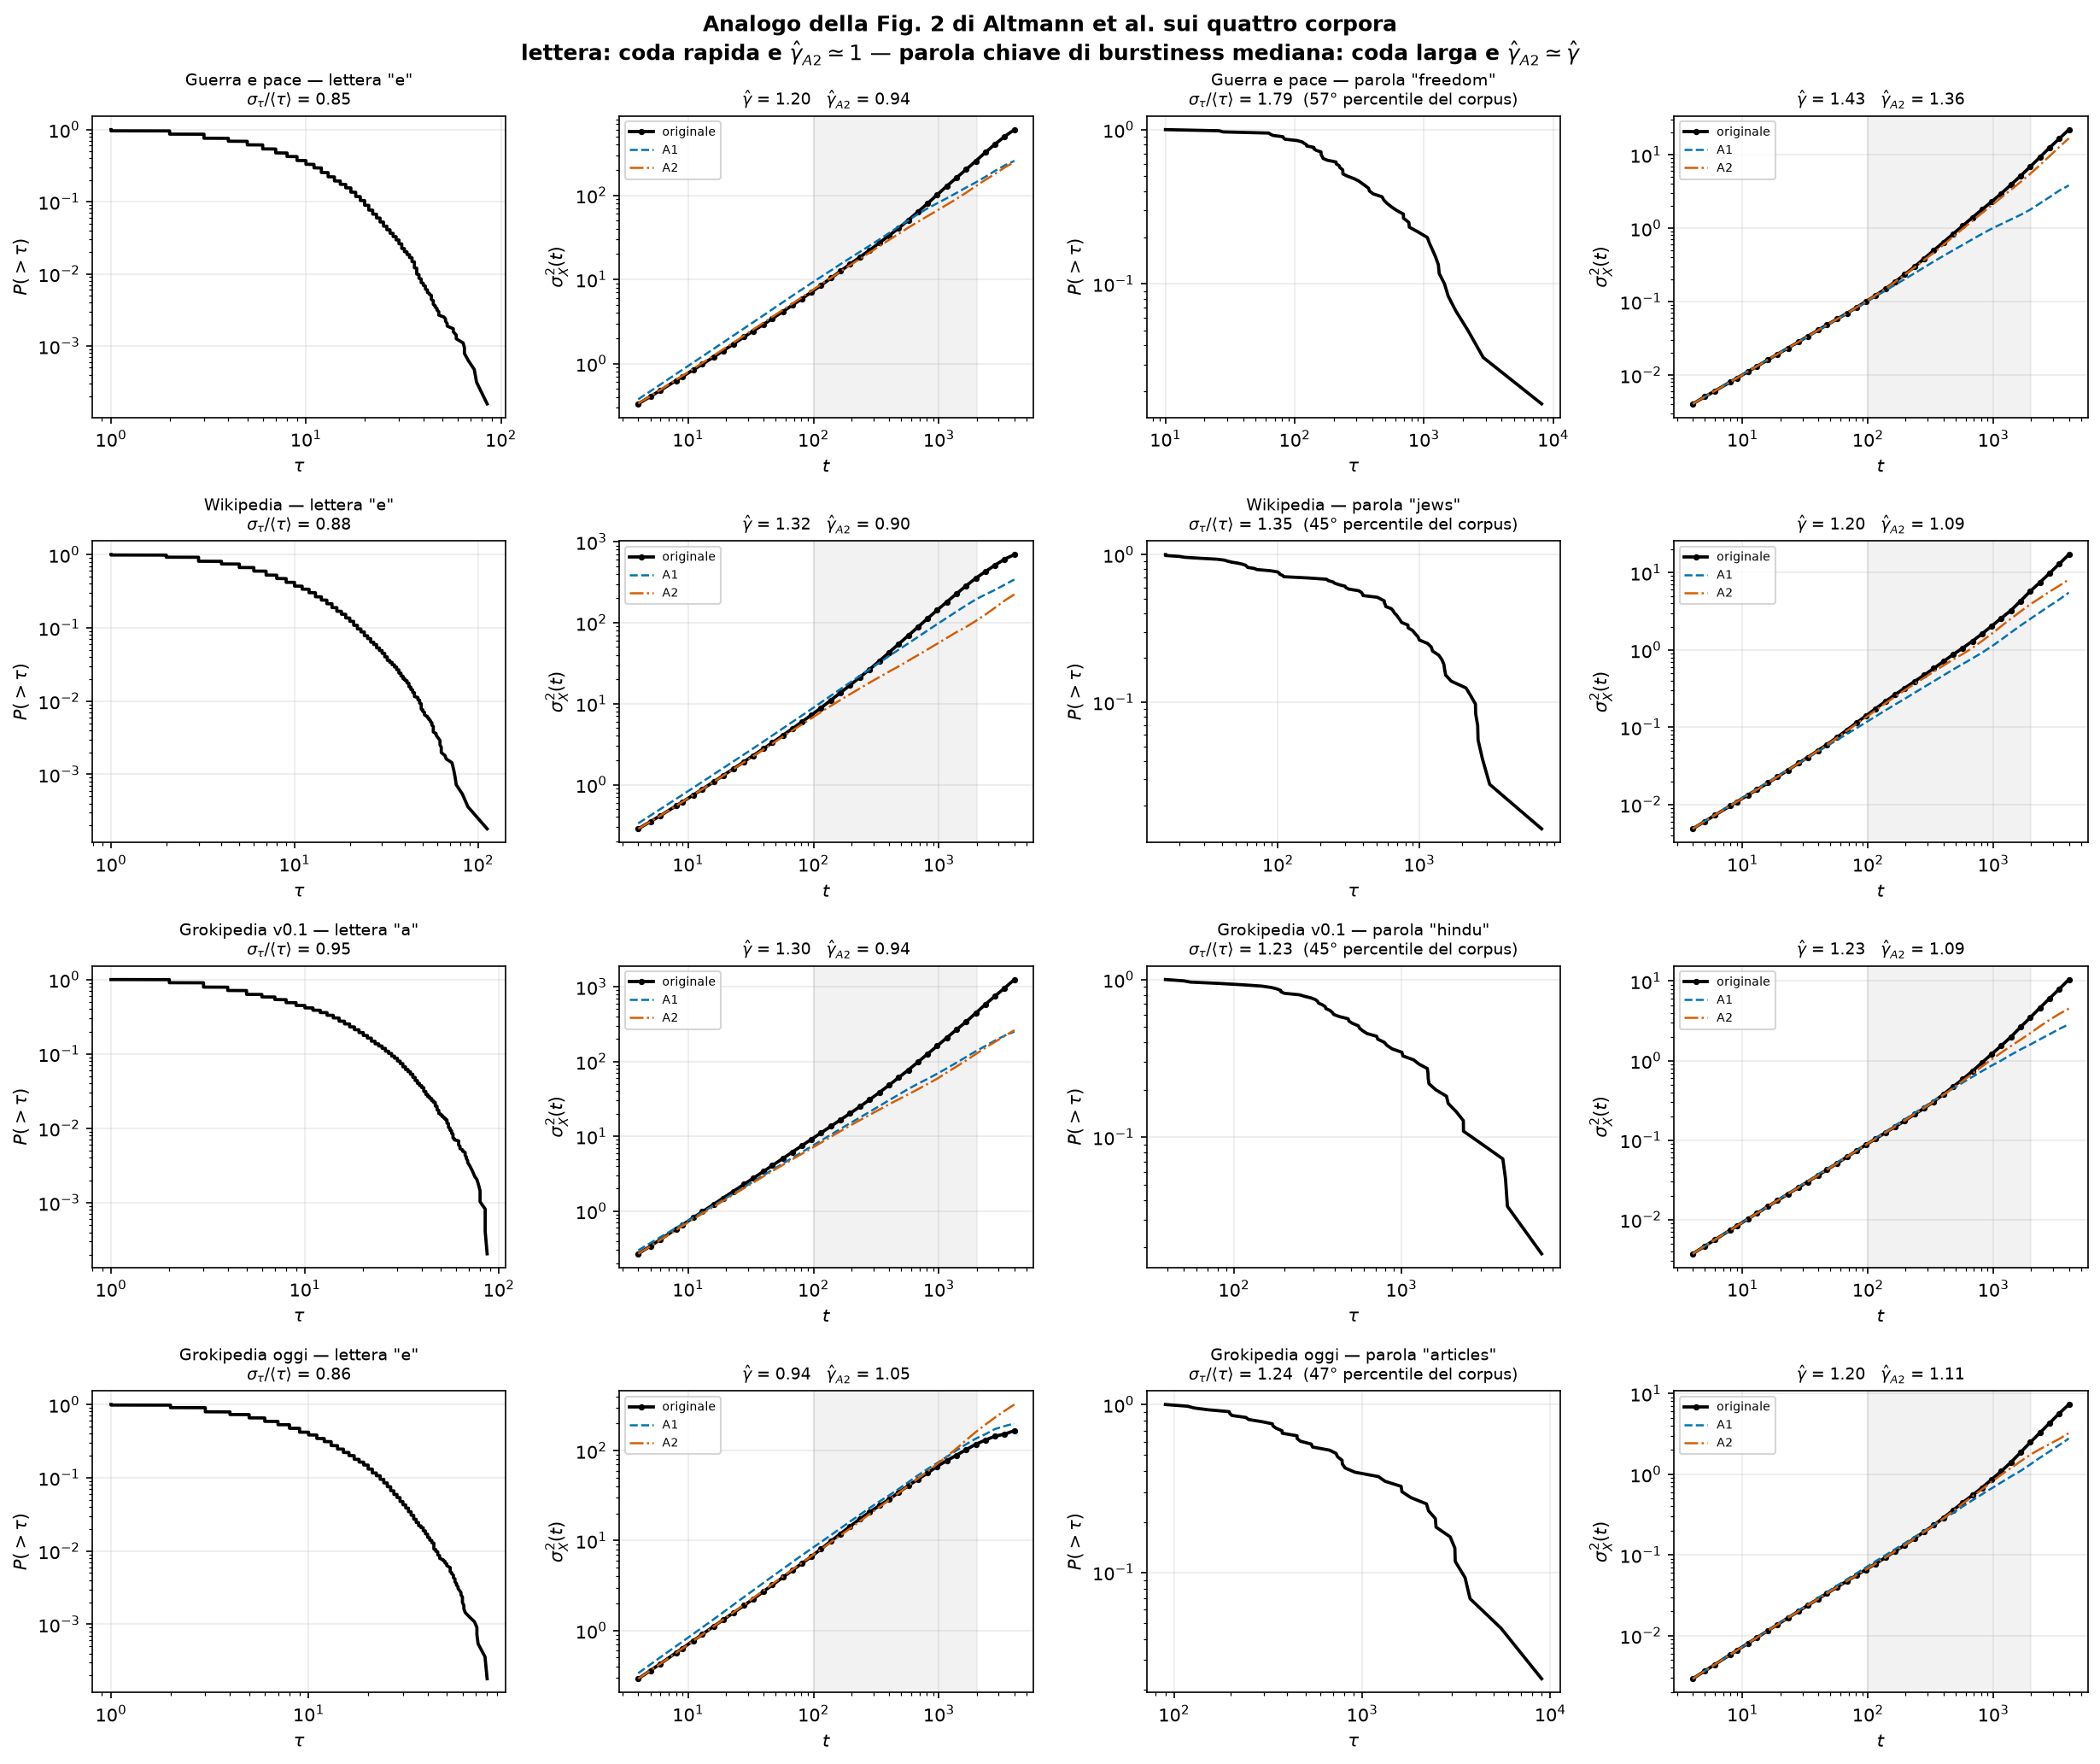
\includegraphics[width=\textwidth]{figure/cap5_altmann_fig2.png}
  \caption{Analogo della Figura~2 di~\cite{altmann2012} sui quattro corpora. Una
  riga per corpus; a sinistra la lettera più frequente del documento, a destra
  la parola chiave di burstiness mediana del corpus fra quelle con almeno
  \num{40} occorrenze, con il suo percentile indicato sopra il pannello. Per
  ciascuna, la distribuzione cumulata degli intervalli $P(>\tau)$ e la crescita
  della varianza del conteggio $\sigma_X^2(t)$, con le curve dei due null model
  del §\ref{sec:null} e la finestra di fit ombreggiata. La lettera ha coda
  rapida e $\hat\gamma_{A2} \simeq 1$; la parola di contenuto ha coda larga e
  $\hat\gamma_{A2}$ prossimo a $\hat\gamma$.}
  \label{fig:altmann-fig2}
\end{figure}

\paragraph{Il soggetto della voce non è una parola di contenuto.}
La parola chiave più ricorrente di un articolo enciclopedico, quella che il
criterio scartato sopra avrebbe selezionato, si comporta in modo opposto a
quello che il §\ref{sec:origini} prevede per il suo livello linguistico. Nella
voce \emph{Alexander the Great} di Wikipedia la parola \emph{alexander} ha
$\sigma_\tau/\langle\tau\rangle = 0.78$; in \emph{Sigmund Freud} di Grokipedia
\emph{freud} ha $0.72$. Sono valori sotto il limite poissoniano, cioè
distribuzioni \emph{più regolari del caso}, mentre la lettera \emph{e} negli
stessi testi dà $0.84$. Il confronto con la lettera non va però fatto sul valore
grezzo. Per un processo casuale in tempo discreto
$\sigma_\tau/\langle\tau\rangle$ non vale esattamente uno, ma tanto meno quanto
più corti sono gli intervalli: il null model A1, applicato alla stessa frequenza
della sequenza osservata, restituisce $0.95$ per la lettera \emph{e}, che ricorre
ogni dieci caratteri, e $1.00$ per una parola chiave, che ricorre ogni
duecento.

\paragraph{Il riferimento casuale dipende dalla frequenza.}
La ragione di quel $0.95$ è che gli intervalli sono numeri interi positivi. Se
le occorrenze sono collocate a caso con probabilità $f$ per carattere, la
distanza fra due consecutive è geometrica, e per la geometrica si ha
$\sigma_\tau/\langle\tau\rangle = \sqrt{1-f}$: il valore tende a uno solo nel
limite di eventi rari. Con $f = 1/10$, la frequenza della lettera \emph{e}, si
ottiene $0.949$; con $f = 1/200$, la frequenza tipica di una parola chiave,
$0.997$. Il valore poissoniano di riferimento non è dunque lo stesso ai due
livelli, ed è più basso proprio dove gli eventi sono più fitti. Confrontare
\emph{alexander} e la lettera \emph{e} sui valori grezzi significherebbe
attribuire alla struttura del testo una differenza che è invece un effetto
della sola frequenza.

Rapportando ciascuna misura al proprio valore casuale l'effetto si toglie, e
resta $0.78$ per \emph{alexander} contro $0.88$ per la lettera: il soggetto
della voce è più regolare di una lettera anche dopo aver tolto l'effetto della
frequenza, e la differenza fra i due, lungi dall'essere prodotta dalla
normalizzazione, ne esce accentuata.

\paragraph{Perché il soggetto si comporta così.}
La ragione è che in prosa enciclopedica il soggetto non è un tema fra altri,
che alterna presenza e assenza lungo il testo, ma il tema unico: compare come soggetto grammaticale di quasi ogni
periodo, e i suoi intervalli ereditano allora la statistica della lunghezza
delle frasi anziché quella dell'alternanza tematica. La verifica è diretta.
Nei sei articoli esaminati il soggetto ricorre una volta ogni $1.4$--$1.7$
frasi, con lo stesso valore in Wikipedia e in Grokipedia. I suoi intervalli sono
quindi lunghezze di frase, e ne ereditano la variabilità: le
lunghezze di frase di quegli articoli hanno
$\sigma_\tau/\langle\tau\rangle$ fra $0.33$ e $0.73$, e il soggetto della voce
si colloca poco sopra, fra $0.54$ e $0.78$, comunque sotto l'unità che
segnerebbe l'assenza di struttura. Per confronto, \emph{natásha} in un segmento
di \emph{Guerra e pace} ricorre una volta ogni $5.1$ frasi e ha
$\sigma_\tau/\langle\tau\rangle = 3.24$: lì la ricorrenza non segue il ritmo del
periodo ma l'alternanza delle scene.

Il soggetto della voce funziona quindi da marcatore sintattico e non semantico,
e la sua ricorrenza è governata dal ritmo del periodo, non dalla persistenza di
un argomento. Non è un difetto della misura ma un tratto del genere
enciclopedico, e va tenuto presente nel confrontare la burstiness lessicale fra
generi diversi: è la ragione per cui la parola mostrata nella
Figura~\ref{fig:altmann-fig2} viene scelta sulla mediana e non sul massimo.

% ---------------------------------------------------------------------
\section{Il divario si apre al livello lessicale}
\label{sec:appaiato}

L'appaiamento per titolo permette un test più stringente del confronto fra
medie. Confrontare la media di Wikipedia con quella di Grokipedia lascia
aperta l'obiezione che le due medie siano calcolate su argomenti diversi, e
che la differenza rifletta il contenuto anziché la scrittura. Il test appaiato
la chiude: per ciascuna delle \num{39} voci, che nei due corpora tratta lo
stesso argomento, si calcola la differenza fra il valore di Grokipedia e
quello di Wikipedia, e si verifica con il test dei ranghi segnati di Wilcoxon
che la mediana di quelle \num{39} differenze sia diversa da zero. Il test è
non parametrico, quindi non assume che le differenze siano distribuite
normalmente, assunzione che con \num{39} osservazioni e distribuzioni
asimmetriche non sarebbe difendibile.

Il test dà, per la versione attuale di Grokipedia,
$-0.167$ sulle parole chiave e $-0.010$ sulle lettere; ai due livelli intermedi
le differenze valgono $-0.037$ per le parole funzione e $-0.157$ per i controlli
appaiati, tutte con significatività inferiore a $10^{-2}$. La versione v0.1 dà
$-0.012$, $-0.039$, $-0.116$ e $-0.133$.

I quattro numeri vanno letti come una scala. Alle lettere Grokipedia e
Wikipedia distano un centesimo di unità di burstiness, cioè circa l'uno per
cento del valore misurato: a quel livello i due corpora sono, in pratica, lo
stesso testo. Alle parole funzione la distanza quadruplica, ma resta piccola in
termini relativi. Ai due livelli lessicali passa a circa sedici centesimi, oltre
un decimo del valore misurato e più di un ordine di grandezza sopra il livello
delle lettere.

La scala ha però un solo gradino, non tre. La differenza fra i livelli
sub-lessicali e quelli lessicali è netta; quella fra i due livelli lessicali non
esiste: $-0.157$ sui controlli a frequenza appaiata contro $-0.167$ sulle parole
chiave sono lo stesso numero. Il testo generato non perde dunque le parole di
contenuto più di quanto perda le altre parole della stessa frequenza. Ciò che i
dati sostengono è che riproduca le regolarità dei livelli bassi e abbassi
uniformemente la burstiness a livello di parola, non che perda selettivamente la
persistenza tematica.

\paragraph{Il divario alla lunghezza di controllo.}
\label{sec:robustezza-neff}
L'intera catena è stata ripetuta a $N_{\mathrm{eff}} = \num{80000}$ caratteri,
lunghezza a cui sopravvivono \num{35} delle \num{39} terne; per isolare
l'effetto della finestra, i valori a \num{60000} sono ricalcolati sulle stesse
\num{35}. Alle lettere e alle parole funzione il divario appaiato è stabile, da
$-0.010$ a $-0.011$ e da $-0.037$ a $-0.045$; ai due livelli lessicali si separa
in direzioni opposte, con i controlli appaiati da $-0.164$ a $-0.195$ e le parole
chiave da $-0.167$ a $-0.130$, quest'ultima con significatività che scende a
$p = 0.027$. Alla lunghezza maggiore il divario sulle parole chiave è dunque
\emph{minore} di quello sui controlli appaiati. Ciò che risulta robusto è il
salto dal livello sub-lessicale a quello lessicale; l'ulteriore crescita fino
alle parole chiave non lo è. Anche l'esponente di coda è instabile fra le due
lunghezze, da $2.19$ a $2.50$ su Grokipedia e da $2.37$ a $2.25$ su Wikipedia,
coerentemente con l'avvertenza del §\ref{sec:coda-risultati}.

La Figura~\ref{fig:altmann-fig3} riporta le stesse sequenze nel piano che
\cite{altmann2012} usa per la propria Figura~3: la burstiness in ascissa e
l'esponente di correlazione in ordinata, un punto per sequenza, con un simbolo
diverso per livello linguistico. La gerarchia vi si legge come una disposizione
spaziale: le lettere, gli spazi e le vocali si addensano in una colonna stretta
attorno a $\sigma_\tau/\langle\tau\rangle \simeq 0.5$, le parole funzione e i
controlli appaiati occupano la regione centrale, le parole chiave si spingono a
destra e in alto. È la stessa gerarchia dei paragrafi precedenti, vista tutta
insieme invece che un livello alla volta.

Il piano rende però visibile anche una proprietà che i confronti per livello
non mostrano, e che è l'osservazione centrale di quel lavoro: l'angolo in
basso a destra è vuoto. Non esistono, cioè, sequenze molto \emph{bursty} e
insieme poco correlate. Sui quattro corpora di questa tesi la regolarità si
quantifica così: delle $451$ sequenze con $\sigma_\tau/\langle\tau\rangle >
1.5$, soltanto $17$, il $3.8\%$, hanno $\hat\gamma < 1.1$, e fra quelle con
burstiness superiore a $2$ l'esponente non scende mai sotto $1.05$. L'angolo
opposto, invece, è popolato: delle $3500$ sequenze sotto il valore poissoniano
$\sigma_\tau/\langle\tau\rangle = 1$, il $15.9\%$ ha $\hat\gamma > 1.2$.

L'asimmetria fra i due angoli è la firma di una relazione a senso unico. La
burstiness produce correlazione, come mostra la~\eqref{eq:eq4}, e una sequenza
con vuoti lunghi non può quindi risultare scorrelata; il viceversa non vale,
perché la correlazione può venire anche dall'ordine degli intervalli e
manifestarsi senza alcuna coda pesante. La correlazione di rango fra le due
quantità è positiva e significativa in tutti e quattro i corpora, da $+0.22$ su
Wikipedia a $+0.36$ sul romanzo. Il meccanismo descritto in~\cite{altmann2012}
sui romanzi si ritrova dunque identico nella prosa enciclopedica e in quella
generata, ed è un risultato indipendente dal divario misurato sopra: riguarda
come le due grandezze si legano fra loro, non quanto valgano.

\begin{figure}[htbp]
  \centering
  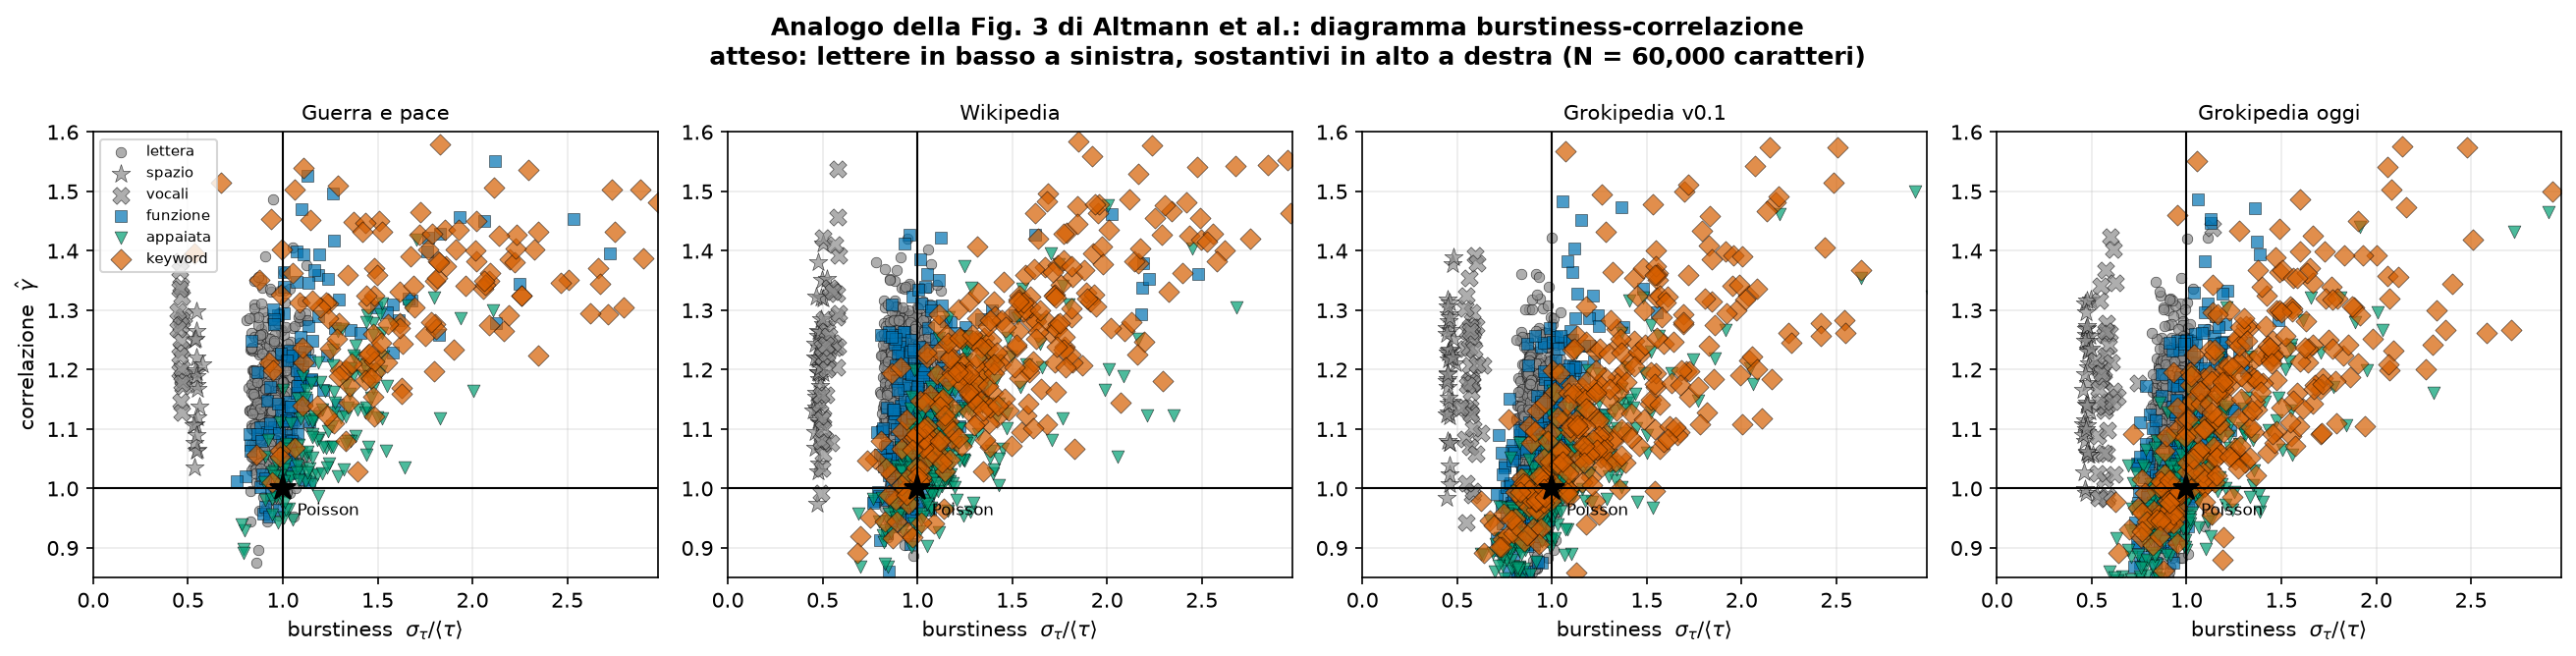
\includegraphics[width=\textwidth]{figure/cap5_altmann_fig3.png}
  \caption{Analogo della Figura~3 di~\cite{altmann2012}: diagramma
  burstiness--correlazione sui quattro corpora, un punto per sequenza. Oltre ai
  quattro livelli usati nel resto del capitolo sono riportati i due livelli
  sub-lessicali tenuti come diagnostica, gli spazi e le vocali. Le linee nere
  segnano il processo di Poisson,
  $\sigma_\tau/\langle\tau\rangle = 1$ e $\hat\gamma = 1$. L'angolo in basso a
  destra è praticamente vuoto in tutti e quattro i corpora: sequenze molto
  bursty e insieme poco correlate non si osservano.}
  \label{fig:altmann-fig3}
\end{figure}

\paragraph{I due quadranti che restano.} La lettura del piano fatta finora
riguarda la diagonale: l'angolo in basso a destra vuoto e quello in alto a
sinistra popolato. Gli altri due separano però i corpora meglio di qualunque
media, e la Figura~\ref{fig:quadranti} li riporta separatamente. Fra le parole
chiave, l'angolo in alto a destra è la posizione canonica
di~\cite{altmann2012}, quella in cui la sequenza è insieme bursty e correlata.
Vi ricade il $91.4\%$ delle sequenze di \emph{Guerra e pace} e l'$87.5\%$ di
quelle di Wikipedia, ma solo il $74.0\%$ di Grokipedia v0.1 e il $77.3\%$
della versione attuale. La differenza finisce quasi interamente nell'angolo
opposto, in basso a sinistra, dove la parola è più regolare di un processo di
Poisson e insieme priva di correlazione a lungo raggio: $0\%$ sul romanzo,
$5.1\%$ su Wikipedia, $15.4\%$ su Grokipedia v0.1 e $14.3\%$ sulla versione
attuale. Una parola chiave generata su sette si trova dunque nell'angolo
opposto a quello canonico, contro una su venti in Wikipedia. Il test appaiato
sulle \num{39} voci conferma che non è un effetto di composizione del
campione: la quota di parole chiave in basso a sinistra cresce in $21$ e $22$
voci su $39$, con differenza mediana $+0.143$ e $p < 10^{-3}$ per entrambe le
versioni.

Due controlli escludono le spiegazioni strumentali. Il null model A1
restituisce $\hat\gamma = 0.983$ in tutti e quattro i corpora, identico alla
terza cifra, quindi la soglia $\hat\gamma = 1$ non è tarata diversamente da un
corpus all'altro; il valore calibrato non è però esattamente uno, cosicché la
soglia è lievemente generosa verso il lato correlato, allo stesso modo per
tutti. E la quota di parole in basso a sinistra resta più alta in Grokipedia
dentro quattro fasce di frequenza su cinque, da $0.159$ contro $0.050$ per le
parole con $26$--$35$ occorrenze a $0.303$ contro $0.076$ per quelle con più di
$80$. Fa eccezione la fascia più bassa, $15$--$25$ occorrenze, dove il rapporto
si inverte, $0.065$ contro $0.200$; lì però le parole chiave di Wikipedia sono
dieci in tutto e la quota è stimata su di esse. Il divario non dipende quindi
dal fatto che le parole chiave di Wikipedia siano più frequenti, salvo nella
fascia in cui il confronto ha meno appoggio.

Guardare dentro il quadrante non rivela più un gruppo omogeneo. Separando le
parole che compaiono nel titolo della voce dalle altre, le $14$ di Wikipedia si
dividono a metà, e le $39$ di Grokipedia si dividono in $18$ soggetti di voce e
$21$ altre parole, prevalentemente aggettivi generici: \emph{economic} in cinque
voci, \emph{military} in tre, \emph{urban} in due. Sono concentrazioni modeste,
e soprattutto non sono più quelle che la lista di parole funzione originaria
lasciava passare: con quella lista, il quadrante conteneva \emph{like} in dodici
voci, \emph{amid} in nove e \emph{including} in sei, cioè i connettivi che
costituiscono il vizio stilistico più evidente del testo generato. Quei termini
sono ora classificati come parole funzione, che è ciò che sono, e il
§\ref{sec:effetto-stoplist} misura quanto la loro presenza fra le parole chiave
alterasse i risultati.

\begin{figure}[htbp]
  \centering
  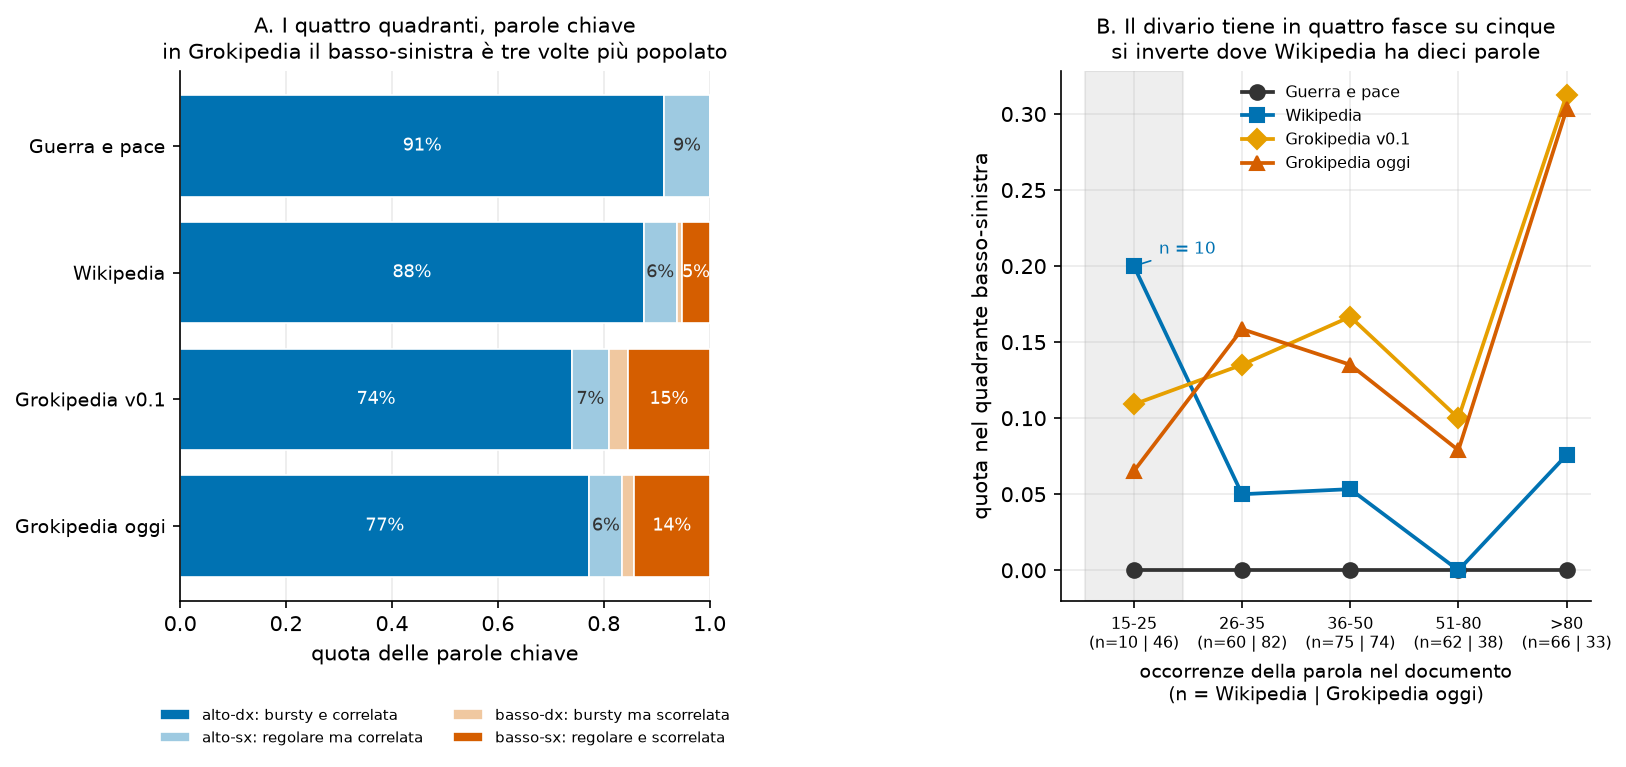
\includegraphics[width=\textwidth]{figure/cap5_quadranti.png}
  \caption{Lettura per quadranti del piano della
  Figura~\ref{fig:altmann-fig3}, sulle sole parole chiave. A: composizione per
  quadrante, un corpus per riga; le quote sotto il $5\%$ non sono etichettate. B:
  quota di parole chiave nel quadrante in basso a sinistra, separando le parole
  per numero di occorrenze nel documento; sotto ciascuna fascia è indicato
  quante parole chiave vi cadono in Wikipedia e in Grokipedia. Il divario tiene
  in quattro fasce su cinque e si inverte nella più bassa, dove Wikipedia ne ha
  dieci in tutto e la fascia è ombreggiata per segnalarlo.}
  \label{fig:quadranti}
\end{figure}

\paragraph{Un effetto di scala da neutralizzare.} Le voci di Grokipedia hanno
frasi sensibilmente
più lunghe di quelle di Wikipedia: $4.38$ frasi ogni mille caratteri contro
$6.92$. Poiché in questo capitolo il tempo è contato in caratteri, la scala
degli intervalli $\tau$ non è la stessa nei due corpora, e un testo con frasi
più lunghe tende ad avere intervalli più lunghi anche a parità di struttura
tematica. Il coefficiente di variazione è un rapporto e non risente di una
dilatazione uniforme dell'asse, ma la dilatazione qui non è uniforme, perché
agisce solo sui livelli definiti su unità linguistiche. Il
§\ref{sec:entropia-intervalli} introduce la misura che elimina il problema;
fino a quel punto il divario va considerato provvisorio.

Il riferimento letterario, infine, non è appaiato per argomento con nessuno dei
tre corpora enciclopedici: entra nei confronti come livello medio e non nei test
appaiati.

% ---------------------------------------------------------------------
\section{Quale meccanismo genera la correlazione}
\label{sec:decomposizione}

Sapere che un testo ha correlazioni a lungo raggio non dice da dove esse
vengano. Il §\ref{sec:null} ha introdotto i due null model che separano le due
origini possibili e la quota di burstiness $q$ della~\eqref{eq:quota}, che vale
circa uno quando la correlazione è interamente spiegata dalla distribuzione
degli intervalli, e circa zero quando è invece l'ordine in cui le occorrenze si
susseguono a produrla.

Il primo pannello della Figura~\ref{fig:decomposizione} riporta $q$ ai quattro
livelli. Sulle lettere il valore è negativo in tutti e quattro i corpora, da
$-0.06$ su Wikipedia a $-0.19$ su Grokipedia v0.1: le lettere sono correlate,
come mostra il $\hat\gamma$ maggiore di uno, ma non sono \emph{bursty}, e la
correlazione viene interamente dall'ordine. Sulle parole chiave il valore sale a
$0.89$ sul romanzo, $0.77$ su Wikipedia, $0.70$ sulla v0.1 e $0.74$ sulla
versione attuale di Grokipedia: qui quasi tutta la correlazione è già contenuta nella
distribuzione degli intervalli. I due livelli intermedi interpolano fra i due
regimi in modo ordinato.

La dissociazione fra il livello dei caratteri e quello del contenuto, che
in~\cite{altmann2012} è osservata su romanzi, si ritrova quindi identica nella
prosa enciclopedica e anche nella prosa generata. Il secondo pannello mostra la
stessa cosa in termini di esponenti: le curve piene sono $\hat\gamma$ e quelle
tratteggiate $\hat\gamma_{A2}$, e la distanza verticale fra le due è il
contributo dell'ordine delle occorrenze. Sulle lettere le due curve sono
separate e la tratteggiata sta all'unità; sulle parole chiave si avvicinano e
salgono insieme.

I valori dei tre corpora enciclopedici sono però troppo vicini perché la
differenza sia interpretabile: fra Wikipedia e Grokipedia vale $0.03$ alla
lunghezza di lavoro e cambia segno a quella di controllo del
§\ref{sec:robustezza-neff}. I dati non consentono quindi di attribuire ai due
corpora un'origine diversa della correlazione, ma soltanto un'intensità diversa.

Sulla riga dei controlli appaiati per Grokipedia, infine, la quota è stimabile
solo su $6$ documenti su $39$ per la versione v0.1 e su $8$ per quella
attuale. La ragione non è un difetto della stima ma la grandezza stessa: $q$
ha $\hat\gamma - 1$ al denominatore, e viene calcolata soltanto dove quel
denominatore supera $0.05$, perché sotto quella soglia il rapporto è dominato
dall'errore. A quel livello i documenti di Grokipedia hanno $\hat\gamma$
mediano pari a $1.003$ per la v0.1 e $1.015$ per la versione attuale, contro
$1.091$ di Wikipedia: le loro sequenze di controllo sono essenzialmente
scorrelate, e non c'è alcuna correlazione da decomporre nelle due origini.
L'esclusione è quindi essa stessa un dato, perché è il livello in cui il testo
generato si avvicina di più al caso, ma il valore di $q$ che sopravvive sui
pochi documenti restanti riguarda proprio quelli in cui una correlazione c'è,
e non va letto come una misura del corpus.

\begin{figure}[htbp]
  \centering
  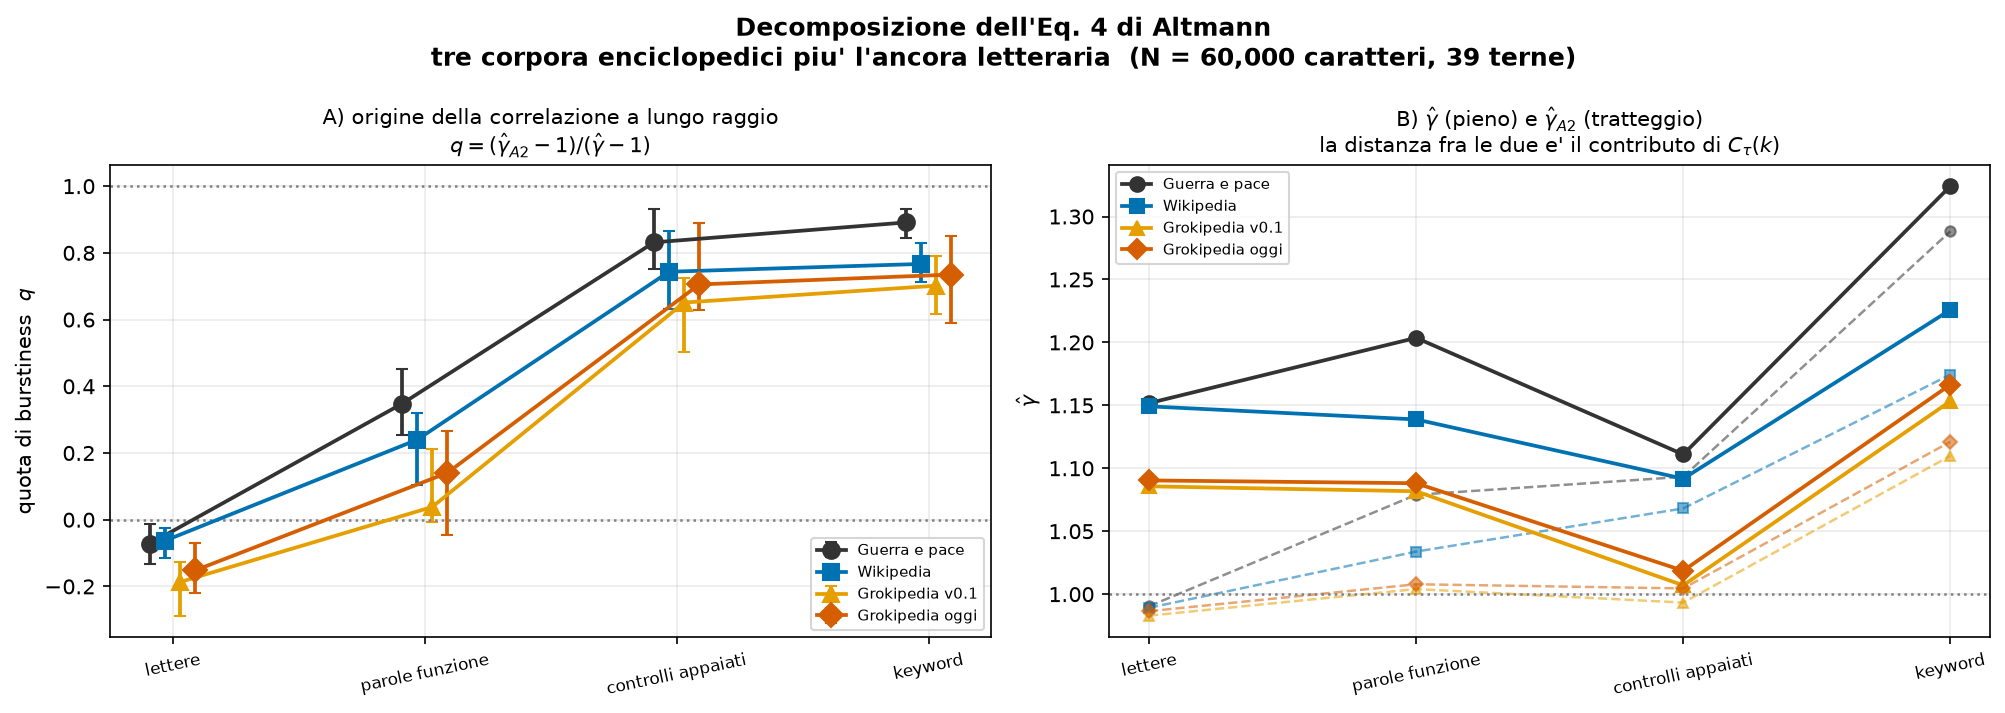
\includegraphics[width=\textwidth]{figure/cap5_decomposizione_eq4.png}
  \caption{Decomposizione della correlazione nelle sue due origini. A: quota
  $q$ della~\eqref{eq:quota} ai quattro livelli linguistici, con intervalli di
  confidenza; $q \simeq 0$ indica correlazione dovuta all'ordine delle
  occorrenze, $q \simeq 1$ correlazione dovuta alla distribuzione degli
  intervalli. B: esponente $\hat\gamma$ (linea piena) e $\hat\gamma_{A2}$
  (tratteggiata) agli stessi livelli; la distanza fra le due curve è il
  contributo della correlazione fra intervalli successivi.}
  \label{fig:decomposizione}
\end{figure}

% ---------------------------------------------------------------------
\section{La coda della distribuzione degli intervalli}
\label{sec:coda-risultati}

Il §\ref{sec:coda} ha osservato che la relazione fra esponente di coda e
esponente di correlazione, nella forma in cui compare in~\cite{altmann2012},
presuppone una distribuzione degli intervalli di cui la coda non viene misurata
ma assunta. Qui la coda viene stimata direttamente, adottando il modello
troncato
\begin{equation}
  p(\tau) \;\sim\; \tau^{-\mu}\,e^{-\tau/\tau_c}
  \label{eq:coda-troncata}
\end{equation}
e determinando $\mu$ e $\tau_c$ per massima verosimiglianza, con intervalli di
confidenza di profilo.

L'analisi della coda comprende, oltre ai quattro livelli usati nel resto del
capitolo, due livelli sub-lessicali aggiuntivi tenuti come diagnostica, le
vocali e gli spazi, per un totale di ventiquattro celle. Il primo risultato
riguarda la forma stessa della distribuzione: il confronto di verosimiglianza
fra la~\eqref{eq:coda-troncata} e una legge di potenza pura rifiuta
quest'ultima in tutte e ventiquattro, con significatività numericamente
indistinguibile da zero. La coda esiste, ma è tagliata.

Il primo pannello della Figura~\ref{fig:coda} riporta $\mu$ ai quattro livelli.
La banda verde segna la regione $2 < \mu < 3$ entro cui la~\eqref{eq:eq8} è
derivata assumendo una legge di potenza pura. Che le stime vi cadano dentro o
fuori non dice nulla sulla convergenza dei momenti: nella
~\eqref{eq:coda-troncata} il taglio li rende finiti per qualunque $\mu$, e il
rifiuto della potenza pura in tutte e ventiquattro le celle toglie il
presupposto sotto cui la banda avrebbe quel significato. Resta un riferimento
utile perché è la regione in cui il paper colloca il proprio valore assunto.
I simboli grigi segnalano le celle in cui il fit degenera in un
esponenziale puro e $\mu$ non è interpretabile, e le linee di collegamento le
saltano. Sono sette celle su sedici: tutti e quattro i corpora sul livello delle
lettere, e i tre corpora enciclopedici su quello delle parole funzione.

Alle parole funzione il romanzo è l'unico dei quattro il cui fit non degenera,
con $\tau_c = 5.3$ contro $1.7$--$1.9$: le sue parole funzione conservano un
tratto di coda a legge di potenza che negli altri tre corpora non esiste, e a
quel livello il coefficiente di variazione dà lo stesso quadro, $1.19$ contro
valori fra $0.97$ e $1.03$ indistinguibili da un processo di Poisson.

Sarebbe naturale leggerlo come una differenza di genere, e il controllo non lo
conferma. Ripetendo la stessa procedura sui tre romanzi inglesi impiegati come
controllo in questo capitolo, il fit sulle parole funzione degenera su
\emph{Moby Dick} ($\tau_c = 1.7$, esattamente il valore dei corpora
enciclopedici) e su \emph{David Copperfield} ($\tau_c = 2.8$), e sopravvive per
poco su \emph{Middlemarch} ($\tau_c = 3.2$); il coefficiente di variazione dà
$1.03$, $1.09$ e $1.08$, cioè valori compresi fra Wikipedia e
\emph{Guerra e pace} e nel primo caso identici a quelli enciclopedici. A questo
livello l'eccezione è quindi del testo e non del genere, come il
§\ref{sec:tre-corpora} osserva anche sul livello delle parole chiave. Il confronto fra i quattro
corpora resta perciò leggibile soltanto sulle parole chiave, dove i valori
stanno fra $1.76$ e $2.37$; sui controlli appaiati tutti e quattro i fit sono al
limite della degenerazione e gli intervalli di confidenza superano l'unità di
ampiezza.

Il confronto con~\cite{altmann2012} chiude qui un cerchio. In quel lavoro $\mu$
non viene stimato ma assunto: per costruire il limite inferiore di $\hat\gamma$
della propria Figura~3 gli autori adottano il valore $\mu = 2.4$. La stima
diretta condotta qui lo colloca dentro l'intervallo di confidenza di tutti e tre
i corpora enciclopedici, e a tre centesimi dal valore centrale di Wikipedia. Il
parametro che quel lavoro doveva postulare risulta dunque misurabile, e il
valore postulato corretto. Il confronto è legittimo perché $\mu$ designa in
entrambi i casi la pendenza della coda nella regione in cui la legge di potenza
vale; ciò che cambia è che qui quella regione è delimitata da un $\tau_c$
stimato anziché estesa all'infinito, e il capoverso seguente misura quanto la
differenza di modello sposti il numero.

Il corpus letterario fa eccezione, con $\mu = 1.76$ e intervallo di confidenza
$[1.40, 2.08]$, e su questo servono due precisazioni, perché il valore cade
sotto la banda $2 < \mu < 3$ entro cui la~\eqref{eq:eq8} è derivata. La prima
è che non è una particolarità di \emph{Guerra e pace}: ripetendo l'intera
procedura su tre altri romanzi inglesi, segmentati e misurati allo stesso
modo, si ottiene $1.51$ su \emph{Moby Dick}, $2.10$ su \emph{Middlemarch} e
$1.96$ su \emph{David Copperfield}, tutti sotto il valore di Wikipedia a ogni
quantile di $x_{\min}$ dall'ottantesimo in su. È un tratto della prosa
letteraria, non del testo scelto, ed è lo stesso fatto che il coefficiente di
variazione registra come burstiness massima: coda più pesante significa
esponente più piccolo.

La seconda è che il valore dipende dal modello con cui lo si stima. Sotto il
modello troncato adottato qui la banda $2 < \mu < 3$ non ha ruolo, perché il
taglio rende media e varianza finite per qualunque $\mu$; sotto il modello a
potenza pura, che è quello di~\cite{altmann2012}, lo stimatore di massima
verosimiglianza sugli stessi dati dà $2.49$ per il corpus letterario, dentro la
banda e a nove centesimi dal valore assunto nel paper. I due numeri non sono in
conflitto: descrivono la stessa coda sotto ipotesi diverse, e la scelta fra le
due è decisa dal rapporto di verosimiglianza, che rifiuta la potenza pura. La
misura non contraddice dunque il valore postulato in quel lavoro; ne circoscrive
il modello.

\begin{figure}[htbp]
  \centering
  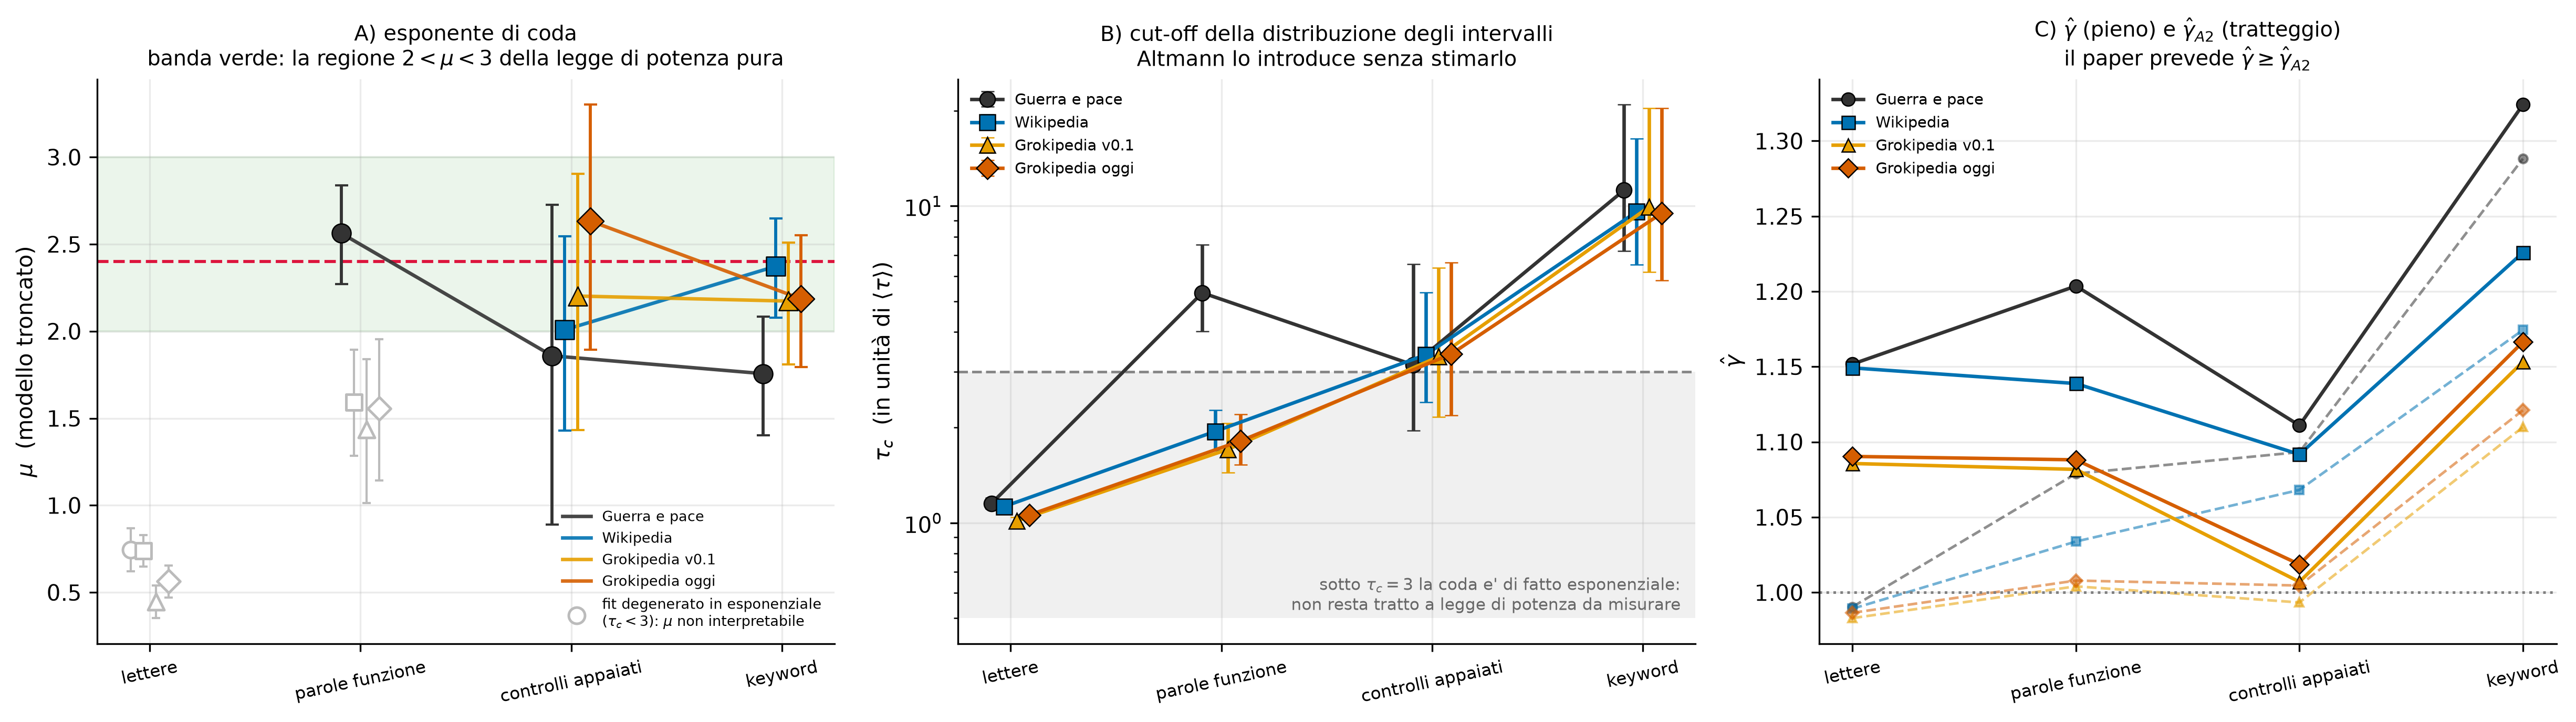
\includegraphics[width=\textwidth]{figure/cap5_esponente_coda.png}
  \caption{Stima diretta della coda della distribuzione degli intervalli. A:
  esponente $\mu$ della~\eqref{eq:coda-troncata} ai quattro livelli, con
  intervalli di confidenza di profilo; la banda verde è la regione $2<\mu<3$ in
  cui è derivata la~\eqref{eq:eq8} per la legge di potenza pura, mentre sotto il
  modello troncato adottato qui i momenti restano finiti per qualunque $\mu$ e
  la banda va letta come riferimento alla letteratura; i simboli grigi sono le
  celle in cui il fit degenera in un esponenziale e $\mu$ non è interpretabile,
  che le linee di collegamento saltano. B: cut-off
  $\tau_c$ agli stessi livelli, in unità dell'intervallo medio e con intervalli
  di confidenza di profilo; sotto la soglia tratteggiata non resta tratto a legge
  di potenza da misurare. C: $\hat\gamma$ (pieno) contro $\hat\gamma_{A2}$
  (tratteggiato) ai quattro livelli. La~\eqref{eq:disug1} è rispettata in tutte
  le celle: la curva piena sta sempre sopra la tratteggiata.}
  \label{fig:coda}
\end{figure}

\paragraph{Perché $\mu$ non serve a confrontare i corpora.}
I quattro valori non vanno però usati per ordinare i corpora, e la
Figura~\ref{fig:verosimiglianza} mostra perché: $\mu$ e $\tau_c$ sono
fortemente correlati, cosicché le regioni di confidenza congiunte sono creste
allungate anziché ellissi compatte e quelle dei tre corpora enciclopedici si
sovrappongono quasi interamente. A ciò si aggiunge la dipendenza dal punto in
cui si decide che la coda cominci: spostando $x_{\min}$ dal settantacinquesimo
al novantacinquesimo percentile $\mu$ passa da $1.65$ a $2.63$ su Wikipedia, una
variazione maggiore di ogni differenza fra corpora, e le curve si incrociano.

Di questa analisi non resta perciò un ordinamento fra corpora. Restano due
risultati, entrambi insensibili alla posizione esatta lungo la cresta: la legge
di potenza pura è rifiutata ovunque, e il cut-off cresce in modo ordinato
salendo nella gerarchia linguistica. Il cut-off è previsto
da~\cite{altmann2012} come conseguenza della discesa lungo quella stessa
gerarchia, e la sua esistenza è qui verificata invece che assunta.

\begin{figure}[htbp]
  \centering
  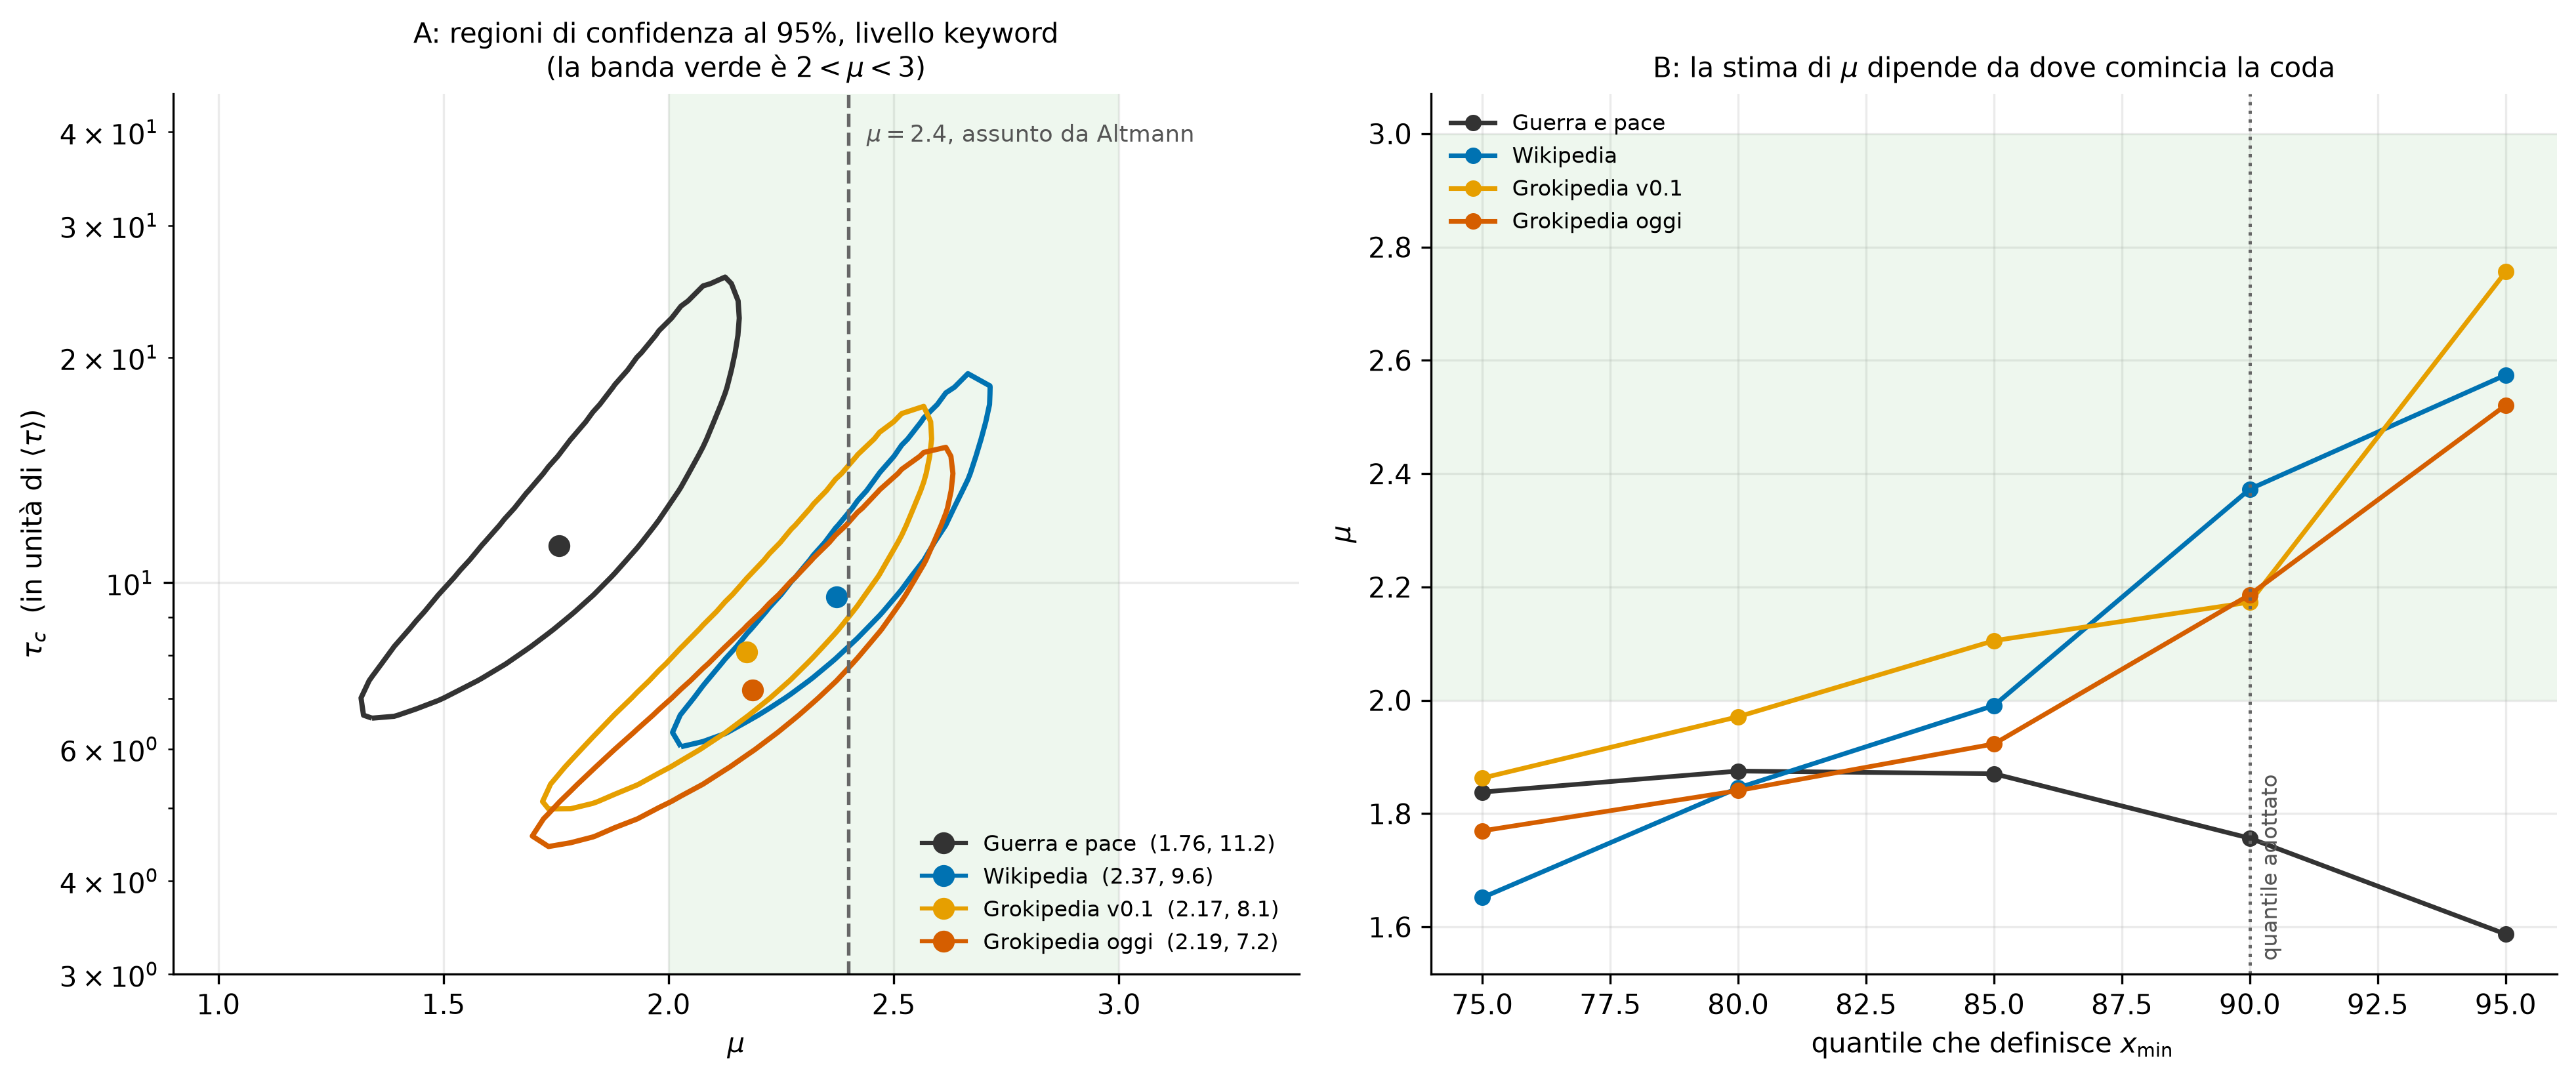
\includegraphics[width=\textwidth]{figure/cap5_verosimiglianza_coda.png}
  \caption{Perché l'esponente di coda non discrimina fra i corpora. A: regioni
  di confidenza congiunte al $95\%$ nel piano $(\mu, \tau_c)$ sul livello delle
  parole chiave, con $x_{\min}$ al novantesimo percentile; l'allungamento delle
  regioni è la correlazione fra i due parametri, e la linea tratteggiata è il
  valore $\mu = 2.4$ assunto in~\cite{altmann2012}. B: stima di $\mu$ al variare
  del quantile che definisce $x_{\min}$; le quattro curve si incrociano, cosicché
  l'ordinamento fra corpora dipende da quella scelta.}
  \label{fig:verosimiglianza}
\end{figure}

\paragraph{Il cut-off e la finestra di osservazione.} Il secondo pannello
della Figura~\ref{fig:coda} riporta $\tau_c$ ai quattro livelli, con
intervalli di confidenza di profilo. È l'altra metà di ciò
che~\cite{altmann2012} introduce senza stimare: il cut-off vi compare come
conseguenza necessaria della discesa nella gerarchia, ma non gli viene mai
assegnato un valore. Cresce in modo ordinato salendo nella gerarchia: circa
$1.1$ volte l'intervallo medio sulle lettere, dove la coda è di fatto già
esponenziale, $3.2$--$3.4$ sui controlli appaiati e $9.5$--$11.2$ sulle parole
chiave. La separazione fra i due livelli superiori è netta. Fra i quattro
corpora, invece, gli intervalli di confidenza si sovrappongono ampiamente:
neppure il cut-off ordina i corpora, e la sola cella in cui la separazione è
significativa è quella delle parole funzione del romanzo, discussa sopra.

Anche $\tau_c$ va poi letto come descrittore relativo alla lunghezza di analisi.
Ripetendo la stima sul romanzo a lunghezze crescenti, da \num{30000} a
\num{480000} caratteri, $\tau_c$ passa da $13.5$ a $94.7$: un fattore sette a
fronte di un fattore sedici sulla finestra, con un andamento non monotono che
scende prima di risalire. Il taglio non è dunque un puro artefatto, perché non
scala proporzionalmente alla finestra, ma non è nemmeno una lunghezza intrinseca
del testo. Sulla stessa serie $\mu$ si stabilizza attorno a $2.0$ alle finestre
maggiori, contro l'$1.76$ misurato alla lunghezza di lavoro: entrambi i
parametri descrivono la coda \emph{a quella lunghezza}, coerentemente con la
regola del §\ref{sec:lunghezza}.

\paragraph{Lo stimatore di Hill.} Dà sistematicamente valori più alti, $2.49$ sul
romanzo contro $1.76$ e circa $3.0$ sugli altri tre corpora contro
$2.2$--$2.4$, perché assume una legge di potenza pura su tutta la coda.
L'assenza di un plateau nel suo grafico diagnostico è ciò che ha motivato
l'adozione del modello troncato, e i suoi valori sono riportati solo a quel
titolo.

% ---------------------------------------------------------------------
\section{Entropia degli intervalli}
\label{sec:entropia-intervalli}

L'effetto di scala dichiarato nel §\ref{sec:appaiato} richiede una misura che
non risenta della lunghezza media delle frasi. È la ragione per cui il
§\ref{sec:entropia-intervalli-def} ha introdotto l'entropia degli intervalli
$J$ della~\eqref{eq:entropia-intervalli}: il logaritmo la rende invariante per
dilatazione dell'asse, cosicché frasi mediamente più lunghe non la spostano, e
la sottrazione del termine poissoniano ne cancella il bias. La grandezza è
risultata calcolabile su \num{5343} sequenze su \num{5617}, il $95\%$ del
totale.

\paragraph{Perché la misura è legittima.}
Trattandosi di una grandezza introdotta qui, la sua adozione va giustificata su
quello che fa e non su un precedente. I due ingredienti sono però entrambi
standard: l'entropia differenziale stimata per spaziature d'ordine è lo
stimatore di~\cite{vasicek1976}, e il confronto di una statistica osservata con
il valore che essa assume su un processo di Poisson di pari intensità è la
costruzione con cui in letteratura si misura la regolarità di una sequenza di
eventi, la stessa su cui poggiano la~\eqref{eq:cv} e il coefficiente
di~\cite{goh2008} usati nel resto del capitolo. Ciò che $J$ aggiunge è
l'invarianza per dilatazione, che nessuna delle due possiede e che serve qui per
una ragione specifica. Il §\ref{sec:entropia-intervalli-def} argomenta perché
debba funzionare; la validazione empirica è alla fine di questa sezione, dove la
stessa parola misurata a lunghezze diverse sposta il coefficiente di variazione
di un fattore tre e $J$ di due decimi di bit.

\paragraph{Che cosa riportano i tre pannelli.}
Il primo pannello della Figura~\ref{fig:entropia} mostra il rapporto fra $J$ e
il coefficiente di variazione sulle parole chiave. Le due misure sono
correlate, come atteso, ma la relazione non è biunivoca: a parità di
coefficiente di variazione i punti dei diversi corpora occupano fasce di $J$
diverse, il che è precisamente ciò che rende utile la seconda misura.

Il secondo pannello riporta $J$ ai quattro livelli. Sulle lettere i quattro
corpora coincidono attorno a $-0.20$, e sulle parole funzione i tre corpora
enciclopedici scendono insieme attorno a $-0.29$, con il romanzo che resta a
$-0.19$: valori negativi indicano intervalli più regolari di un
processo di Poisson. Sui due livelli superiori i corpora si separano, e sulle
parole chiave i corpora umani stanno sopra il valore poissoniano e quelli
generati vi si appoggiano: $J$ vale $+0.061$ sul romanzo e $+0.092$ su
Wikipedia, contro $-0.001$ su Grokipedia v0.1 e $-0.011$ sulla versione
attuale, questi ultimi due indistinguibili da zero. Le due enciclopedie generate
si collocano dunque sul valore poissoniano, mentre quella umana ne sta sopra:
gli intervalli fra parole chiave di Grokipedia non sono più regolari del caso,
semplicemente non sono più \emph{bursty} di esso. Il terzo pannello riporta la
distribuzione per documento e mostra che la separazione, pur con code
sovrapposte, riguarda l'intero corpus e non alcune voci.

\paragraph{La coda inferiore è fatta di soggetti di voce.}
La coda inferiore di quel pannello merita però un controllo, perché il cambio
di segno è ciò su cui l'affermazione precedente poggia. Le sequenze con $J$
più basso sono parole chiave a pieno titolo, nomi propri e non lessico di
servizio sfuggito alla lista chiusa, ma sono quasi tutte la stessa cosa: il
soggetto della voce. Fra le venti sequenze di $J$ minore, in Grokipedia
quattordici sono il soggetto dell'articolo, e in Wikipedia diciotto:
\emph{churchill}, \emph{newton}, \emph{paris}, \emph{freud}, \emph{mandela}. È
il fenomeno del §\ref{sec:tre-corpora}, che $J$ registra come gli altri
indicatori, e non è un difetto della classificazione.

Ha però una conseguenza sul cambio di segno. Escludendo i soggetti delle voci,
$54$ sequenze su $273$ in Grokipedia e $57$ in Wikipedia, tutti e tre i
corpora enciclopedici passano sopra il valore poissoniano: $+0.175$ su
Wikipedia e $+0.070$ su Grokipedia. Il divario appaiato sopravvive, $-0.087$
bit con $p < 10^{-3}$, e con esso la conclusione del paragrafo; non sopravvive
invece la lettura per segno, perché il segno negativo di Grokipedia è prodotto
dai soggetti delle voci, che il §\ref{sec:tre-corpora} ha già mostrato essere
marcatori sintattici e non semantici. Ciò che distingue i due corpora è quanto
$J$ vale, non da che parte dello zero cade.

\paragraph{Il divario appaiato.}
I confronti appaiati confermano il divario: sulle parole chiave la differenza
mediana fra Grokipedia attuale e Wikipedia vale $-0.105$ bit e quella fra la
v0.1 e Wikipedia $-0.077$ bit, entrambe con significatività inferiore a
$10^{-3}$. Sulle lettere e sulle parole funzione, per contro, le differenze sono
positive e non significative. Poiché $J$ non risente della diversa lunghezza
delle frasi, questo risultato conferma il divario del §\ref{sec:appaiato}
senza risentire di quell'effetto, ed è il punto in cui la conclusione principale
del capitolo diventa difendibile.

\paragraph{Perché il divario è più ampio sui controlli.}
Il divario è però più ampio sui controlli appaiati, $-0.209$ bit, che sulle
parole chiave, e la ragione sta in che cosa siano quei controlli. Il controllo
di una parola chiave è la parola di frequenza più vicina fra quelle che restano
dopo aver tolto le parole chiave stesse, i nomi propri e le sei parole funzione
selezionate; poiché le parole chiave sono per costruzione le più frequenti del
loro tipo, ciò che resta a quelle frequenze è in larga parte lessico di
servizio. I controlli più ricorrenti sono infatti \emph{by}, \emph{from},
\emph{with} e \emph{as} in Wikipedia, e \emph{like}, \emph{but}, \emph{that} e
\emph{this} in Grokipedia. È il livello in cui il testo generato si distingue di
più: le sue parole di servizio sono distribuite quasi uniformemente,
$J = -0.165$, mentre quelle di Wikipedia conservano un residuo di
addensamento, $J = +0.053$.

\paragraph{Composizione e stile, in parti quasi uguali.}
Le due liste di controlli sono però diverse fra loro, e la differenza potrebbe
misurare quali parole vengono selezionate anziché come sono distribuite. Le due
cause si separano restringendo il confronto alle parole che compaiono fra i
controlli di entrambi i corpora. Sono ventisei, e dodici raggiungono almeno tre
voci per corpus. Su queste il divario resta: la differenza mediana di $J$ vale
$-0.091$ bit con $p = 0.043$, e le quattro parole più spostate sono
\emph{with} ($-0.060$ contro $-0.414$), \emph{as} ($+0.227$ contro $-0.106$),
\emph{this} ($-0.005$ contro $-0.301$) e \emph{from} ($+0.057$ contro $-0.225$).
Il divario fra le medie dei due corpora, $-0.218$ bit, si scompone dunque in
$-0.128$ attribuibili alla distribuzione delle stesse parole e $-0.091$ alla
diversa composizione delle due liste, cioè in parti quasi uguali. Il valore
differisce di un centesimo dal $-0.209$ citato sopra perché quello è la mediana
delle differenze voce per voce e questo la differenza fra le medie.

La parte attribuibile alla composizione ha un contenuto proprio. I controlli di
Wikipedia sono preposizioni e ausiliari legati alla struttura del periodo, come
\emph{by}, \emph{was}, \emph{with} e \emph{for}; quelli di Grokipedia sono in
prevalenza connettivi di discorso, come \emph{like}, \emph{but}, \emph{that} e
\emph{over}. La parte attribuibile alla distribuzione descrive invece un
meccanismo: in Wikipedia una preposizione come \emph{from} si addensa dove il
contenuto la richiede, in una sezione biografica più che in una tecnica, e i suoi
intervalli ereditano il ritmo delle sezioni; in Grokipedia la stessa parola
ricorre a cadenza quasi costante lungo tutto l'articolo. Il segno negativo di $J$
dice che quella cadenza è più regolare di quella di un processo casuale, non
soltanto meno addensata.

Una verifica interna conferma la lettura. Nei controlli di Wikipedia il $93\%$
delle parole appartiene alla lista chiusa e dà $J = +0.043$, mentre il restante
$7\%$ dà $+0.188$: la classe grammaticale della parola cambia il risultato. In
Grokipedia le due quote valgono $-0.151$ e $-0.182$, indistinguibili fra loro.
Nel testo generato la regolarità degli intervalli non dipende da che tipo di
parola si stia guardando, ed è la stessa compressione uniforme della variabilità
lessicale che il §\ref{sec:sintesi-cap5} indica come conclusione del capitolo,
osservata al livello in cui si manifesta con più forza.

\paragraph{Stabilità rispetto alla lunghezza di analisi.}
Una validazione indipendente riguarda la dipendenza dalla lunghezza. Passando
da \num{40000} caratteri al romanzo intero, il coefficiente di variazione della
parola \emph{prince} cambia di un fattore $3.08$, mentre il suo $J$ si sposta di
$0.21$ bit; per la parola \emph{pierre} il coefficiente cambia di un fattore
$3.49$ e $J$ di $0.08$ bit. I due numeri non sono direttamente confrontabili,
perché il coefficiente di variazione è un rapporto e $J$ un logaritmo: uno
spostamento di $0.21$ bit corrisponde a un fattore $2^{0.21} = 1.16$ sulla
dispersione efficace degli intervalli, e uno di $0.08$ bit a un fattore $1.06$.
Riportate alla stessa scala, le due derive stanno nel rapporto di $2.7$ e $3.3$
in favore di $J$. La nuova misura è dunque circa tre volte più stabile rispetto
alla lunghezza di analisi di quella che sostituisce, il che ne conferma
l'utilità al di là del problema specifico per cui era stata introdotta.

\begin{figure}[htbp]
  \centering
  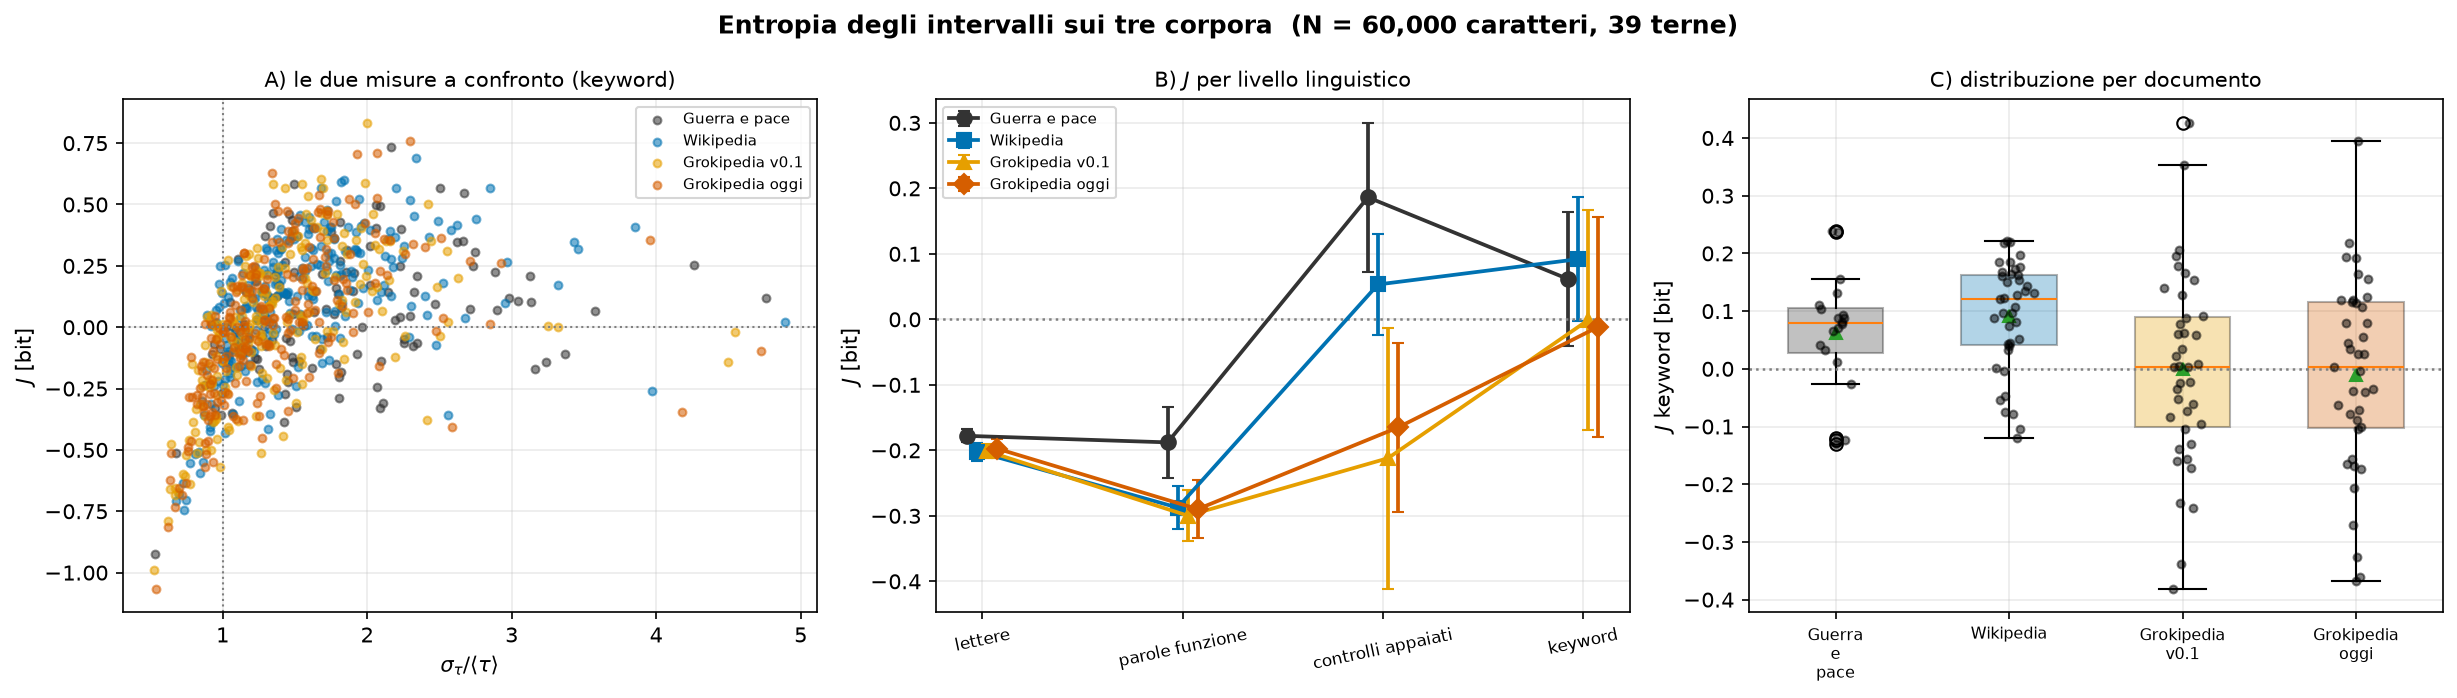
\includegraphics[width=\textwidth]{figure/cap5_entropia_intervalli.png}
  \caption{Entropia degli intervalli. A: relazione fra $J$ e coefficiente di
  variazione sulle parole chiave, un punto per sequenza. B: $J$ ai quattro
  livelli linguistici, con deviazioni standard fra testi; valori negativi
  indicano intervalli più regolari di un processo di Poisson. C: distribuzione
  di $J$ sulle parole chiave documento per documento. La misura è invariante per
  dilatazione dell'asse dei caratteri e non risente quindi della diversa
  lunghezza delle frasi nei due corpora enciclopedici.}
  \label{fig:entropia}
\end{figure}

% ---------------------------------------------------------------------
\section{Quanto pesa la definizione dei livelli lessicali}
\label{sec:effetto-stoplist}

Il paragrafo \emph{Come vengono separati i livelli lessicali} del
§\ref{sec:scelte} ha documentato l'estensione della lista chiusa di parole funzione da
\num{133} a \num{215} voci e la ragione per cui era necessaria. Questa sezione
riporta di quanto si spostano i risultati, perché lo spostamento non è
trascurabile e la scelta deve restare verificabile.

Il pannello A della Figura~\ref{fig:effetto-stoplist} riporta quali parole la
lista originaria lasciava passare fra le parole chiave di Grokipedia, e in
quante voci ciascuna: nell'elenco corrispondente di Wikipedia non ne compare
nessuna, e le sue sette parole sono distinte fra loro, ciascuna in una sola
voce.

\begin{table}[htbp]
  \centering
  \begin{tabular}{lcccc}
    \toprule
    & \multicolumn{2}{c}{lista originaria} & \multicolumn{2}{c}{lista estesa} \\
    \cmidrule(lr){2-3}\cmidrule(lr){4-5}
    & Wikipedia & Grok. oggi & Wikipedia & Grok. oggi \\
    \midrule
    keyword più bursty del controllo & $0.685$ & $0.630$ & $0.692$ & $0.740$ \\
    idem, su $\hat\gamma$ & $0.736$ & $0.663$ & $0.747$ & $0.791$ \\
    $\sigma_\tau/\langle\tau\rangle$ keyword & $1.530$ & $1.289$ & $1.536$ & $1.379$ \\
    divario appaiato, keyword & \multicolumn{2}{c}{$-0.230$} & \multicolumn{2}{c}{$-0.167$} \\
    divario appaiato, controlli & \multicolumn{2}{c}{$-0.122$} & \multicolumn{2}{c}{$-0.157$} \\
    $J$ keyword & $+0.086$ & $-0.069$ & $+0.092$ & $-0.011$ \\
    $\mu$ keyword & $2.38$ & $2.52$ & $2.37$ & $2.19$ \\
    quadrante basso-sinistra & $5.1\%$ & $24.5\%$ & $5.1\%$ & $14.3\%$ \\
    \bottomrule
  \end{tabular}
  \caption{Effetto della definizione dei livelli lessicali sui risultati del
  capitolo. Le righe dei divari appaiati riportano un solo valore perché
  misurano la differenza fra i due corpora. Le lettere e le parole funzione non
  compaiono perché nessuna parola cambia livello a quelle altezze: i loro valori
  coincidono a tutte le cifre riportate nel capitolo.}
  \label{tab:effetto-stoplist}
\end{table}

La Tabella~\ref{tab:effetto-stoplist} riporta il confronto. Tre risultati
cambiano in modo sostanziale. Il primo è il test interno: con la lista
originaria Grokipedia sembrava battere il proprio controllo appaiato meno spesso
di Wikipedia, e l'ordinamento fra i corpora appariva netto; con la lista estesa
l'ordine si inverte, e la differenza fra le due enciclopedie sparisce. Il
pannello B della figura mostra i due esiti sovrapposti. Il secondo è l'entropia
degli intervalli, il cui valore sulle parole chiave passa da $-0.069$ a
$-0.011$, cioè da un cambio di segno netto a uno indistinguibile da zero. Il
terzo è l'esponente di coda, che su Grokipedia scende da $2.52$ a $2.19$,
avvicinandosi a quello di Wikipedia anziché allontanarsene.

Restano invece stabili il divario appaiato complessivo, che si riduce da
$-0.230$ a $-0.167$ senza perdere significatività, il coefficiente di variazione
delle parole chiave, e l'intera decomposizione della~\eqref{eq:eq4}. Non si
muovono di una cifra, come è ovvio, i livelli delle lettere e delle parole
funzione.

La lezione metodologica vale al di là di questo caso. La distinzione fra
parole di contenuto e parole di servizio è la premessa dell'intero protocollo
di~\cite{altmann2012}, e viene qui operata da una lista chiusa che il paper
non specifica. Quando i corpora confrontati hanno abitudini lessicali diverse,
e un modello linguistico ne ha rispetto a un redattore umano, una lista
incompleta non introduce un rumore simmetrico: sposta sistematicamente in un
solo corpus il confine fra i due livelli, e produce un divario che non c'è.

\begin{figure}[htbp]
  \centering
  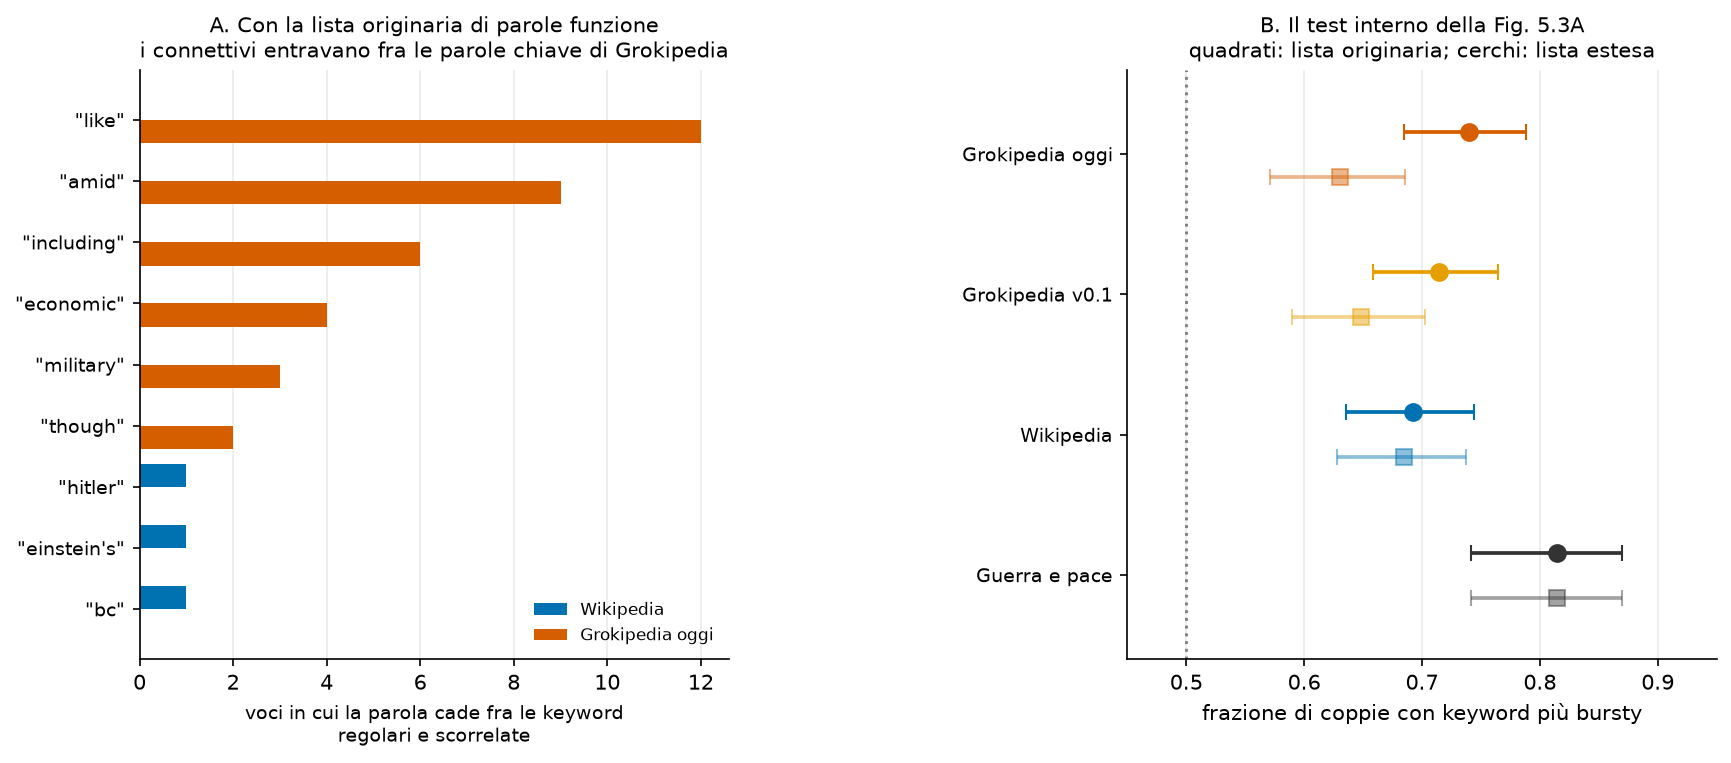
\includegraphics[width=\textwidth]{figure/cap5_effetto_stoplist.png}
  \caption{Effetto della definizione dei livelli lessicali. A: con la lista di
  funtori originaria, quali parole cadevano fra le parole chiave classificate
  come regolari e scorrelate, contate come numero di voci in cui ciò accadeva;
  le prime tre di Grokipedia sono connettivi, e in Wikipedia non compaiono. B:
  il test interno della Figura~\ref{fig:tre-corpora}A con le due
  classificazioni, quadrati per la lista originaria e cerchi per quella estesa,
  con intervalli di confidenza al $95\%$.}
  \label{fig:effetto-stoplist}
\end{figure}

% ---------------------------------------------------------------------
\section{Che cosa il testo generato non riproduce}
\label{sec:sintesi-cap5}

Il testo generato possiede correlazioni a lungo raggio, e ai livelli bassi della
gerarchia linguistica le possiede quasi nella stessa misura del testo umano:
sulle lettere i quattro corpora sono indistinguibili per coefficiente di
variazione, per entropia degli intervalli e per quota di burstiness, e sulle
parole funzione la differenza è piccola, benché significativa. Al livello delle parole il divario si apre, e vale più di un ordine
di grandezza rispetto a quello misurato sui caratteri.

Il divario non distingue però le parole che portano il contenuto dai controlli a
frequenza appaiata. I due valori sono quasi uguali alla lunghezza di lavoro,
$-0.157$ e $-0.167$, e si invertono a quella di controllo
(§\ref{sec:robustezza-neff}); e il test che chiede se la parola chiave superi il
proprio controllo \emph{dentro lo stesso testo} dà a Grokipedia un esito pari a
quello di Wikipedia, anzi lievemente migliore. Il meccanismo descritto
in~\cite{altmann2012} è dunque presente nel testo generato, e con la stessa
efficacia: ciò che manca è l'ampiezza con cui le parole, di contenuto e non, si
addensano.

Non si tratta dunque di una persistenza tematica assente, perché la distinzione
fra parole tematiche e parole ordinarie il modello la produce; si tratta di una
compressione uniforme della variabilità lessicale, che riduce la burstiness di
tutte le parole senza alterare il rapporto fra le une e le altre. Vale ancora la
distinzione posta nel §\ref{sec:intro-linguaggio} fra riprodurre le proprietà
statistiche del linguaggio e riprodurre il meccanismo che le genera, ma
applicata a un livello più basso di quanto la prima lettura suggerisse.

Ciò che il capitolo misura è la distanza fra due enciclopedie appaiate titolo
per titolo, e null'altro. Il deficit è osservato su Grokipedia, cioè su un unico
sistema generativo, in un unico dominio e in una sola lingua: nulla di quanto
riportato qui stabilisce che sia una proprietà dei modelli linguistici in
generale anziché di quel sistema. Il Capitolo~\ref{cap:risultati1} non offre un
appoggio indipendente su questo punto: misura un altro corpus, con grandezze
che non arrivano al livello a cui il divario si manifesta.

%
%  Tre lunghezze di analisi con corpora diversi, da non confondere:
%    fattibilità  50 000 caratteri, 40 voci  (§5.2)
%    analisi      60 000 caratteri, 39 terne (§5.3--5.7)
%    robustezza   80 000 caratteri, 35 terne (§5.8)
% =====================================================================

\chapter{Burstiness lessicale in corpora umani e generativi}
\label{cap:risultati2}

% ---------------------------------------------------------------------
\section{Perché un secondo corpus}
\label{sec:perche-wiki}

Questo capitolo nasce da un esito negativo del precedente. Il
§\ref{sec:fallimenti} ha mostrato che dei \num{242} documenti generati lungo lo
sweep soltanto due non ricadono in alcuna modalità di degenerazione, ed entrambi
si trovano a $T = 1.0$. Il protocollo introdotto nel §\ref{sec:burst} è però un
protocollo semantico: richiede di individuare in ciascun testo le parole che ne
portano il contenuto e di misurare come si distribuiscono le distanze fra le
loro occorrenze successive. Su un testo che ripete lo stesso ciclo di parole, o
su una sequenza degenerata nel senso opposto, 
quelle distanze si calcolano ancora ma non misurano più la
persistenza di un tema. Applicare il protocollo al corpus dello sweep
restituirebbe numeri privi di contenuto.

Il confronto viene quindi spostato su un dominio in cui la qualità del testo
non è una variabile. Wikipedia e Grokipedia trattano le stesse voci, la prima
scritta da esseri umani e la seconda generata da un modello linguistico, ed
entrambe producono prosa espositiva ben formata. Appaiare le due enciclopedie
per titolo tiene inoltre fisso l'argomento trattato: la voce
\emph{Albert Einstein} di Wikipedia e quella di Grokipedia parlano della stessa
cosa, e qualunque differenza nella statistica degli intervalli non può essere
attribuita a un argomento diverso. I corpora sono descritti nel §\ref{sec:corpora}, e le
due versioni di Grokipedia nel §\ref{sec:paternita}.

Il romanzo di riferimento resta nell'analisi come ancora letteraria: è il
dominio su cui il protocollo è stato formulato, e serve a dire quanto la prosa
enciclopedica si discosti già di per sé dal caso studiato in origine.

% ---------------------------------------------------------------------
\section{Il protocollo regge sulla prosa enciclopedica}
\label{sec:fattibilita}

Prima di confrontare due enciclopedie occorre stabilire che l'effetto da
confrontare esista nella prima. Il protocollo di Altmann è stato costruito e
validato su romanzi, e la prosa enciclopedica ha una struttura diversa: non ha
trama, procede per sezioni tematiche dichiarate da titoli, e la persistenza di
un argomento vi si manifesta in modo più rigido. Che le parole di contenuto vi
risultino più \emph{bursty} dei propri controlli non è quindi scontato.

La verifica è stata condotta su \num{40} voci di Wikipedia troncate a
\num{50000} caratteri, contro \num{20} segmenti del romanzo della stessa
lunghezza: è la fase di fattibilità della Tabella~\ref{tab:fasi}, l'unica del
capitolo a impiegare quella lunghezza e quel numero di voci, e i suoi
denominatori non vanno confusi con quelli delle sezioni successive. La
Figura~\ref{fig:wiki-fattibilita} ne riporta l'esito. Il primo
pannello confronta ciascuna parola chiave con il proprio controllo appaiato in
frequenza e riporta la quota di confronti vinti dalla parola chiave: il valore
$0.5$ corrisponde all'assenza di effetto. Su Wikipedia la quota vale
$197/280 = 0.704$ per il coefficiente di variazione e $216/280 = 0.771$ per
l'esponente di correlazione, con estremi inferiori degli intervalli di
confidenza pari a $0.65$ e $0.72$: l'effetto esiste. Sul romanzo le stesse
quote valgono $104/140 = 0.743$ e $123/140 = 0.879$, cioè sono più alte, ma la
differenza non annulla il segnale enciclopedico.

Il secondo pannello mostra da dove viene quel segnale, ed è utile precisare
come i suoi valori siano costruiti, perché la stessa procedura vale per tutte
le figure per livello del capitolo. Dentro ciascun testo si selezionano più
sequenze per livello: diciannove lettere, sei parole funzione, sette parole
chiave e i sette controlli appaiati. Per ognuna si misura
$\sigma_\tau/\langle\tau\rangle$ sui suoi intervalli. I valori delle sequenze
dello stesso livello si mediano poi dentro il testo, ottenendo un
numero per coppia (testo, livello); infine si media su tutti i testi del
corpus, ed è questo secondo valore a comparire nel pannello, con la barra
d'errore data dalla deviazione standard fra testi. Con questa costruzione il
coefficiente di variazione $CV$ cresce salendo lungo i quattro livelli in entrambi
i corpora e con lo stesso andamento: le lettere stanno sotto l'unità, cioè si
distribuiscono in modo più regolare di un processo di Poisson, mentre le
parole chiave arrivano a $1.51$ su Wikipedia e a $1.62$ sul romanzo. Il terzo
pannello riporta la distribuzione dei singoli testi attorno a quelle medie e
mostra che la sovrapposizione fra i due corpora è ampia, con mediane vicine e
code che si intersecano.

Il rapporto fra le due burstiness delle parole chiave vale $0.93$: la prosa
enciclopedica è meno \emph{bursty} del romanzo, ma dello stesso ordine. Il protocollo
regge, e il confronto con Grokipedia ha un segnale da rilevare.

\begin{figure}[htbp]
  \centering
  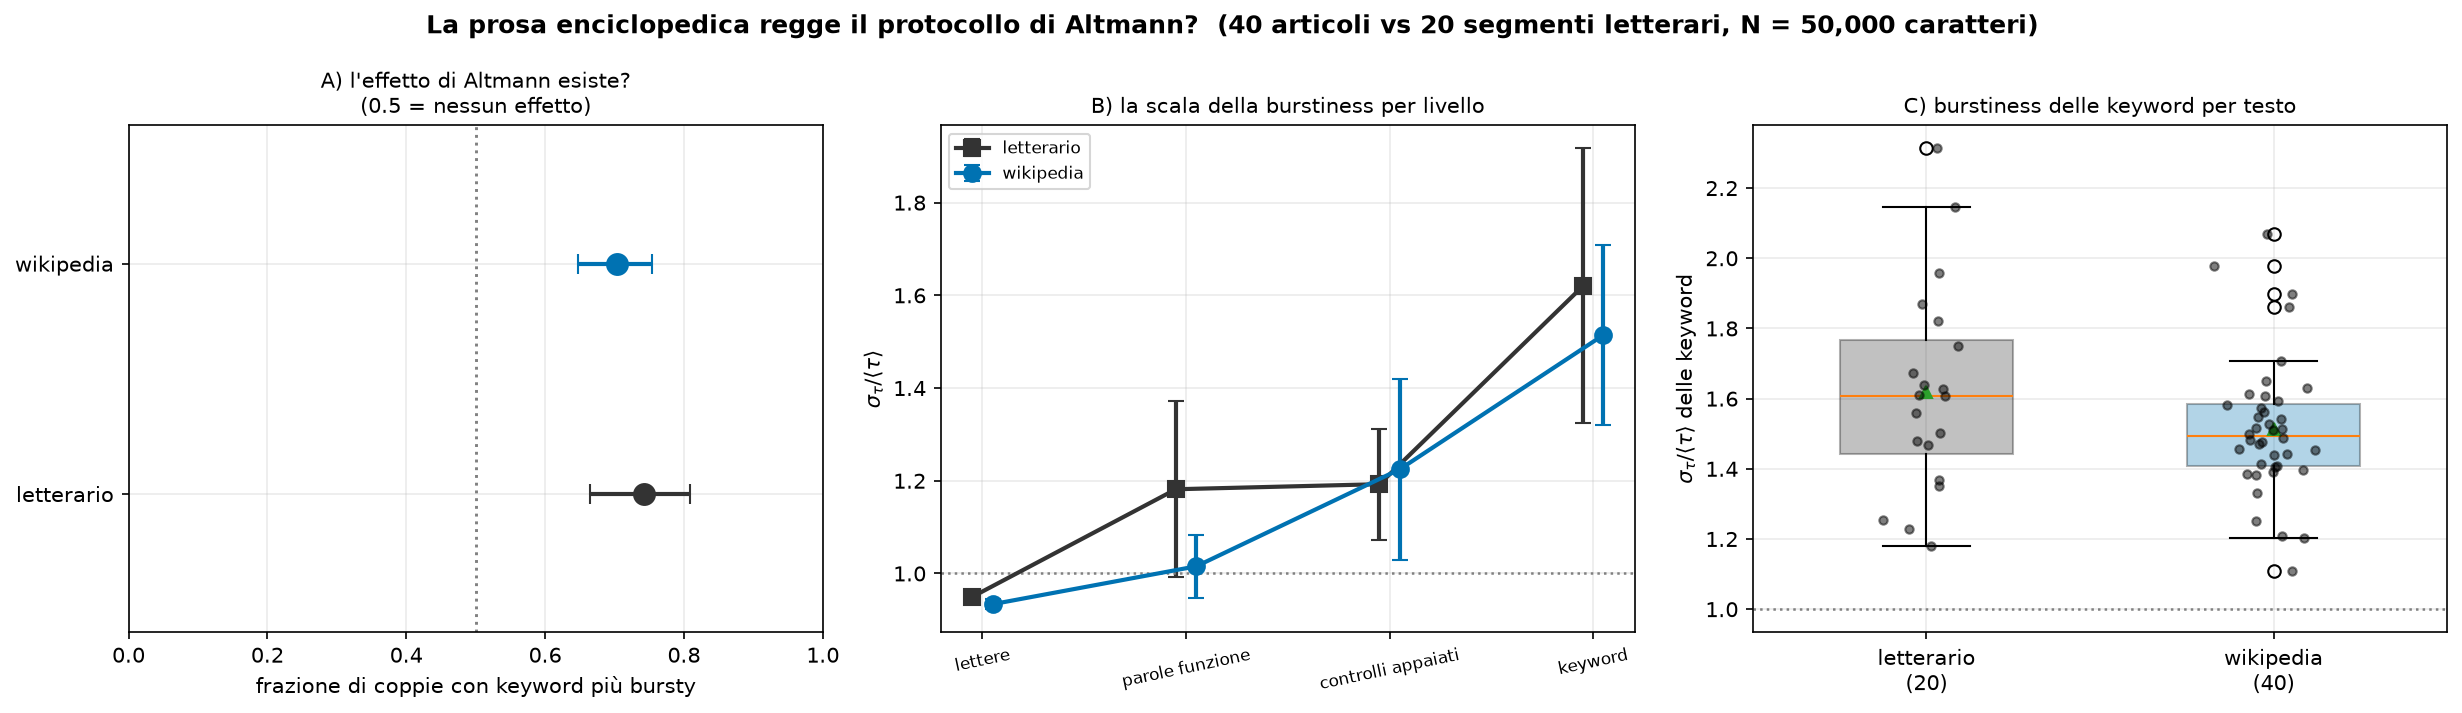
\includegraphics[width=\textwidth]{figure/cap5_wiki_altmann.png}
  \caption{Test di fattibilità del protocollo su prosa enciclopedica, condotto
  su \num{40} voci di Wikipedia e \num{20} segmenti letterari a \num{50000}
  caratteri. A: quota di confronti in cui la parola chiave supera il proprio
  controllo appaiato in frequenza, con intervallo di confidenza al $95\%$; la
  linea punteggiata a $0.5$ è l'assenza di effetto. B: coefficiente di
  variazione degli intervalli ai quattro livelli linguistici. C: distribuzione
  della burstiness delle parole chiave testo per testo. Questa è l'unica figura
  del capitolo costruita su \num{40} voci e \num{50000} caratteri; tutte le
  successive usano \num{39} terne e \num{60000} caratteri.}
  \label{fig:wiki-fattibilita}
\end{figure}

% ---------------------------------------------------------------------
\section{L'effetto nei tre corpora}
\label{sec:tre-corpora}

L'analisi principale confronta Wikipedia, le due versioni di Grokipedia e
l'ancora letteraria su \num{39} terne complete, troncate a \num{60000}
caratteri. La voce esclusa è \emph{Buddhism}, per la ragione riportata nel
§\ref{sec:paternita}: la sua versione v0.1 è ricopiata da Wikipedia, e in un
disegno appaiato un titolo che cade in un corpus deve cadere in tutti.

\paragraph{La finestra su cui l'esponente è stimato.}
L'esponente di correlazione $\hat\gamma$ è ottenuto interpolando
la~\eqref{eq:sigma} nell'intervallo fisso $t \in (100, 2000)$ caratteri.
\cite{altmann2012} adotta invece una regola relativa e ferma la finestra
all'uno per cento della lunghezza del testo. Le due scelte non sono ordinabili
una volta per tutte: applicata ai romanzi interi che quel lavoro analizza la
regola relativa dà un tetto dell'ordine di \num{10000} caratteri, molto più
largo di quello adottato qui; applicata alle finestre da \num{60000} caratteri
di questo capitolo dà $t < 600$, molto più stretto. L'intera catena è stata
ripetuta anche con la seconda. Il
livello medio di $\hat\gamma$ si abbassa di qualche centesimo, sulle parole
chiave da $1.23$ a $1.18$ per Wikipedia e da $1.32$ a $1.22$ per il romanzo,
ma l'ordinamento fra i corpora resta identico a tutti e quattro i livelli. Il
divario appaiato fra Grokipedia attuale e Wikipedia sulle parole chiave passa
da $-0.049$ a $-0.076$, cioè si accentua invece di ridursi, e resta
significativo in entrambi i casi. Le conclusioni di questo capitolo non
dipendono dunque dalla finestra scelta.

\paragraph{Tre modi di leggere il confronto.}
La Figura~\ref{fig:tre-corpora} riporta i tre modi in cui il confronto può
essere letto. Il primo pannello ripete il test del paragrafo precedente sui
quattro corpora: la quota di confronti vinti dalle parole chiave vale
$114/140 = 0.814$ sul romanzo, $189/273 = 0.692$ su Wikipedia,
$195/273 = 0.714$ su Grokipedia v0.1 e $202/273 = 0.740$ su Grokipedia nella
versione attuale. Ripetendo lo stesso test sull'esponente di correlazione
$\hat\gamma$ anziché sulla burstiness, la quota di confronti vinti dalle parole
chiave vale $0.907$ sul romanzo, $0.747$ su Wikipedia, $0.769$ su Grokipedia
v0.1 e $0.791$ su Grokipedia nella versione attuale.
L'effetto esiste ovunque, con tutti e quattro gli
intervalli di confidenza interamente sopra $0.5$, ed è massimo sul romanzo;
fra le due enciclopedie, però, non distingue: i valori di Grokipedia sono anzi
lievemente superiori a quelli di Wikipedia, con intervalli che si sovrappongono.
La domanda a cui questo pannello risponde è se la parola chiave superi il
proprio controllo a frequenza appaiata dentro lo stesso testo, e la
risposta è che ciò accade con la stessa frequenza nei due corpora enciclopedici.
Il deficit di Grokipedia, misurato dai pannelli successivi, non riguarda dunque
l'esistenza del meccanismo ma il livello assoluto della burstiness.

Il secondo pannello mostra il coefficiente di variazione ai quattro livelli e
rende visibile dove la differenza si concentra. Sulle lettere i quattro corpora
sono indistinguibili, tutti compresi fra $0.922$ e $0.950$, e sulle parole
funzione la separazione resta modesta, da $0.967$ a $1.192$. Il divario si apre
ai due livelli lessicali: sui controlli appaiati il romanzo raggiunge $1.262$,
Wikipedia $1.190$ e le due versioni di Grokipedia $1.044$ e $1.055$; sulle
parole chiave rispettivamente $1.789$, $1.536$, $1.387$ e $1.379$. 
Il terzo pannello riporta la stessa quantità testo per testo,
e mostra che la separazione non è l'effetto di pochi articoli anomali: le
distribuzioni di Wikipedia e di Grokipedia si sovrappongono, ma le loro mediane
differiscono di circa $0.25$ e la coda superiore di Wikipedia è più popolata.

\begin{figure}[htbp]
  \centering
  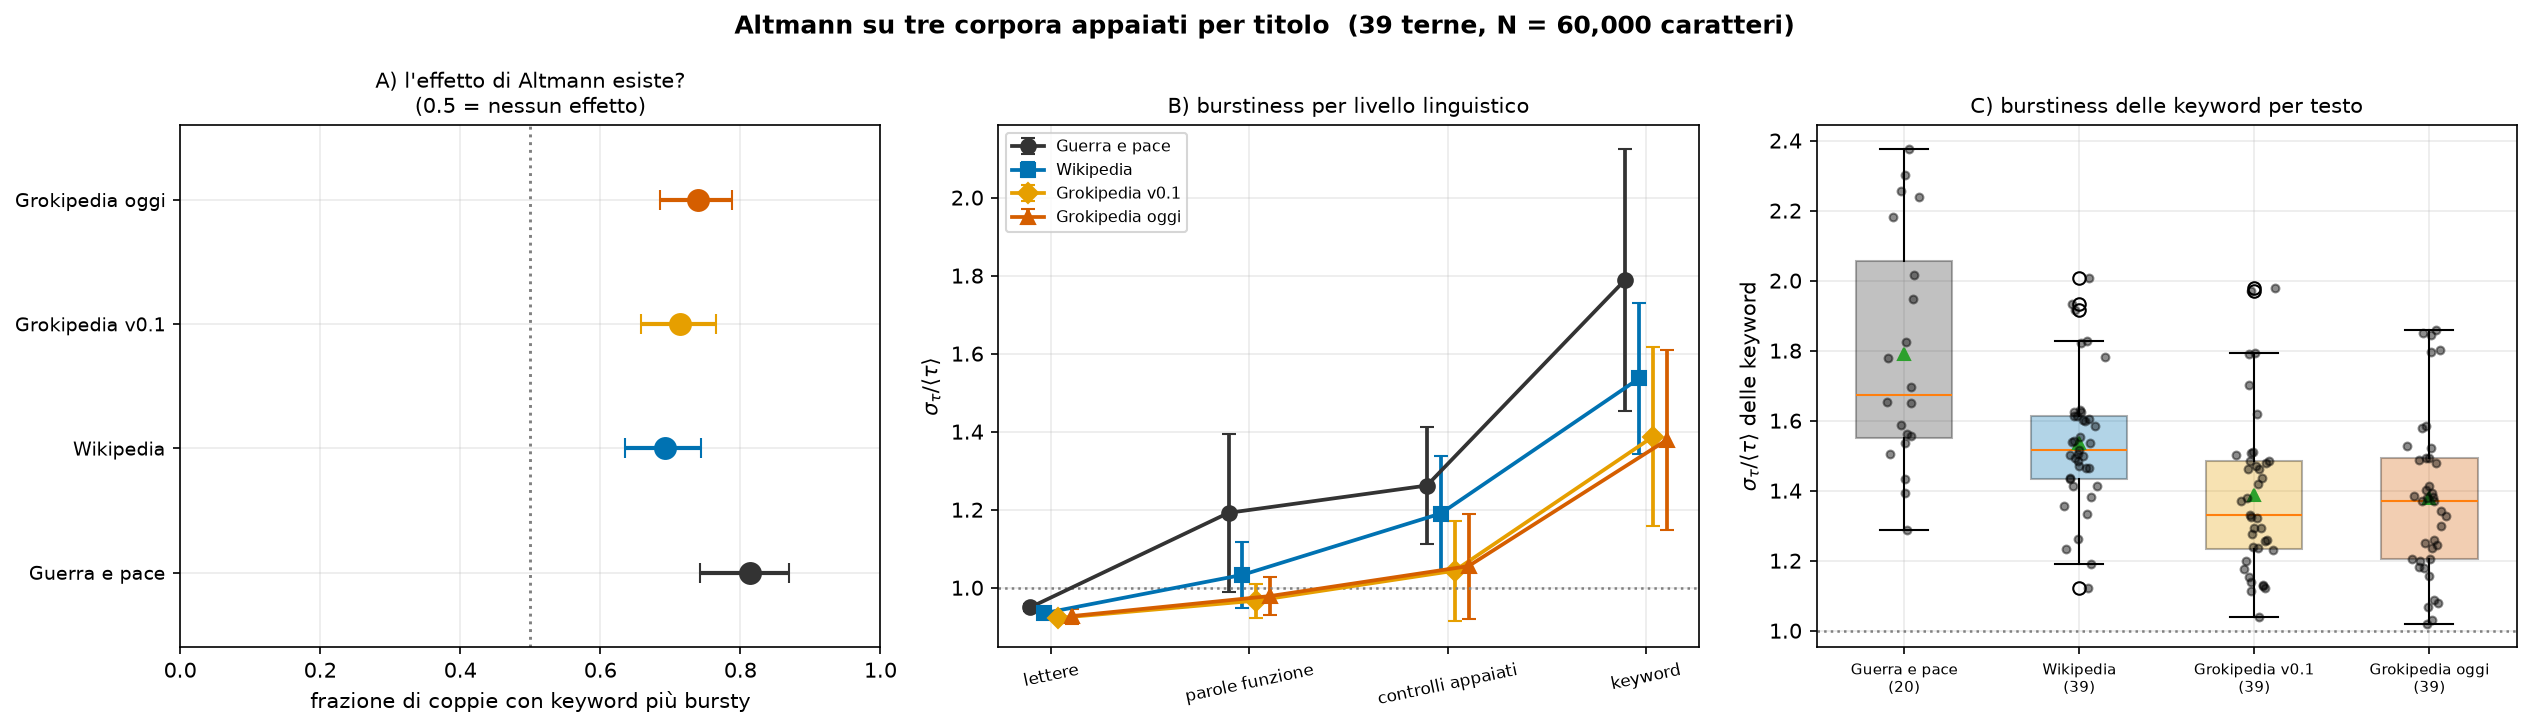
\includegraphics[width=\textwidth]{figure/cap5_tre_corpora.png}
  \caption{Il protocollo di Altmann sui quattro corpora, \num{39} terne
  appaiate per titolo a \num{60000} caratteri. A: quota di confronti vinti dalle
  parole chiave, con intervallo di confidenza al $95\%$. B: coefficiente di
  variazione degli intervalli ai quattro livelli linguistici; le barre sono
  deviazioni standard fra testi. C: burstiness delle parole chiave testo per
  testo, con mediana, quartili e singoli punti sovrapposti. Il numero di testi
  per corpus è indicato sotto ciascuna colonna.}
  \label{fig:tre-corpora}
\end{figure}

\paragraph{L'ancora letteraria è un testo, non un genere.} Il primato del
romanzo sui due livelli lessicali non sopravvive al cambio di testo. Ripetendo
l'intera misura su tre altri romanzi inglesi trattati esattamente come
\emph{Guerra e pace}, cioè \emph{Moby Dick}, \emph{Middlemarch} e \emph{David
Copperfield}, gli stessi impiegati come controllo nel
§\ref{sec:coda-risultati}, sulle parole chiave si ottiene $1.55$, $1.54$ e
$1.63$, cioè valori sostanzialmente pari a quello di Wikipedia e ben al di
sotto dell'$1.79$ di \emph{Guerra e pace}; alle parole funzione si ottiene
$1.03$, $1.08$ e $1.09$, contro l'$1.19$ del romanzo di riferimento e l'$1.03$
di Wikipedia. La distanza fra prosa letteraria e prosa enciclopedica non è
dunque un fatto generale, e l'ancora letteraria di questo capitolo va letta
per ciò che è: un termine di paragone concreto, non la misura di un genere.
Nulla di ciò che segue vi poggia, perché il risultato del capitolo è un
confronto appaiato fra le due enciclopedie, dove il romanzo non entra.

Il null model A1 restituisce un esponente medio di $0.983$ su tutte le celle,
in accordo con l'unità che deve dare per costruzione: la procedura di stima si
comporta come nel §\ref{sec:validazione} anche su questi corpora.

\paragraph{L'analogo della Figura~2 di~\cite{altmann2012}.}
La Figura~\ref{fig:altmann-fig2} riproduce sui quattro corpora la costruzione
con cui~\cite{altmann2012} presenta il proprio risultato principale, e permette
di verificarne l'aderenza riga per riga. Per ogni corpus vengono mostrate una
lettera e una parola di contenuto, ciascuna con la distribuzione cumulata degli
intervalli e con la crescita della varianza del conteggio, accanto alle stesse
curve calcolate sui due null model.

\paragraph{Quale parola mostrare.} La scelta della parola da mostrare pone un
problema che il caso della lettera non ha. Selezionare la parola chiave più
ricorrente del corpus, che è il criterio più immediato, produce oggetti
strutturalmente diversi nei due tipi di prosa: in un romanzo pesca il nome di
un personaggio, presente solo nelle scene in cui il personaggio compare,
mentre in un'enciclopedia pesca il soggetto della voce, che ricorre in quasi
ogni frase. Le due parole finirebbero alle code opposte delle rispettive
distribuzioni di burstiness, al $96$ e al $2$ percentile, e la figura
confronterebbe due casi estremi anziché due casi tipici. La parola mostrata è
quindi quella con $\sigma_\tau/\langle\tau\rangle$ più vicino alla mediana del
proprio corpus, fra quelle con almeno \num{40} occorrenze; il percentile
effettivo è riportato sopra ciascun pannello e sta fra $45$ e $57$ in tutti e
quattro i corpora. Il caso escluso ha però un interesse proprio, ed è ripreso
subito dopo la figura.

\paragraph{Che cosa mostrano le quattro righe.}
Il comportamento è allora quello descritto nel §\ref{sec:origini}, e vale su
tutte e quattro le righe. Sulla lettera la cumulata decade rapidamente e
l'esponente del null model A2 si dispone attorno all'unità, $0.94$ sul romanzo,
$0.90$ su Wikipedia, $0.94$ sulla v0.1 e $1.05$ sulla versione attuale di
Grokipedia, perché a quel livello la burstiness non contribuisce. Lo scarto
massimo da uno vale un decimo, ed è quanto ci si attende su una singola
sequenza: aggregando tutte le \num{2603} sequenze di livello letterale dei
quattro corpora $\hat\gamma_{A2}$ vale fra $0.983$ e $0.990$, con una
dispersione fra sequenze di $0.044$, cosicché i quattro valori della figura
stanno tutti entro due deviazioni standard dall'unità. Un solo caso per corpus
non permette dunque una lettura più fine di così.

Sulla parola di contenuto la cumulata ha coda larga, con
$\sigma_\tau/\langle\tau\rangle$ fra $1.23$ e $1.79$, e $\hat\gamma_{A2}$
resta sopra l'unità e più vicino a $\hat\gamma$ che nel caso della lettera:
$1.36$ contro $1.43$ sul romanzo, $1.09$ contro $1.20$ su Wikipedia, $1.09$
contro $1.23$ sulla v0.1 e $1.11$ contro $1.20$ sulla versione attuale. Una
parte della correlazione passa cioè attraverso la distribuzione degli
intervalli, e la frazione è massima sul romanzo. La figura mostra il
meccanismo su un caso per corpus e non va letta come misura del divario fra
corpora: quella richiede l'aggregato del §\ref{sec:decomposizione}, perché su
una singola parola la differenza fra i due esponenti è dominata dal rumore di
stima. Lo si vede nella riga di Grokipedia attuale, dove sulla lettera
$\hat\gamma = 0.94$ scende sotto $\hat\gamma_{A2} = 1.05$, cosa che
sull'aggregato di quel livello, dove il rumore si media, non accade.

La lettera \emph{e} in \emph{Guerra e pace} dà qui un coefficiente di
variazione pari a $0.85$ contro lo $0.83$ della didascalia della Figura~2
di~\cite{altmann2012}, il che vale come controllo indipendente delle
procedure: la stessa quantità, misurata sullo stesso testo da un codice
diverso, coincide entro due centesimi.

\begin{figure}[htbp]
  \centering
  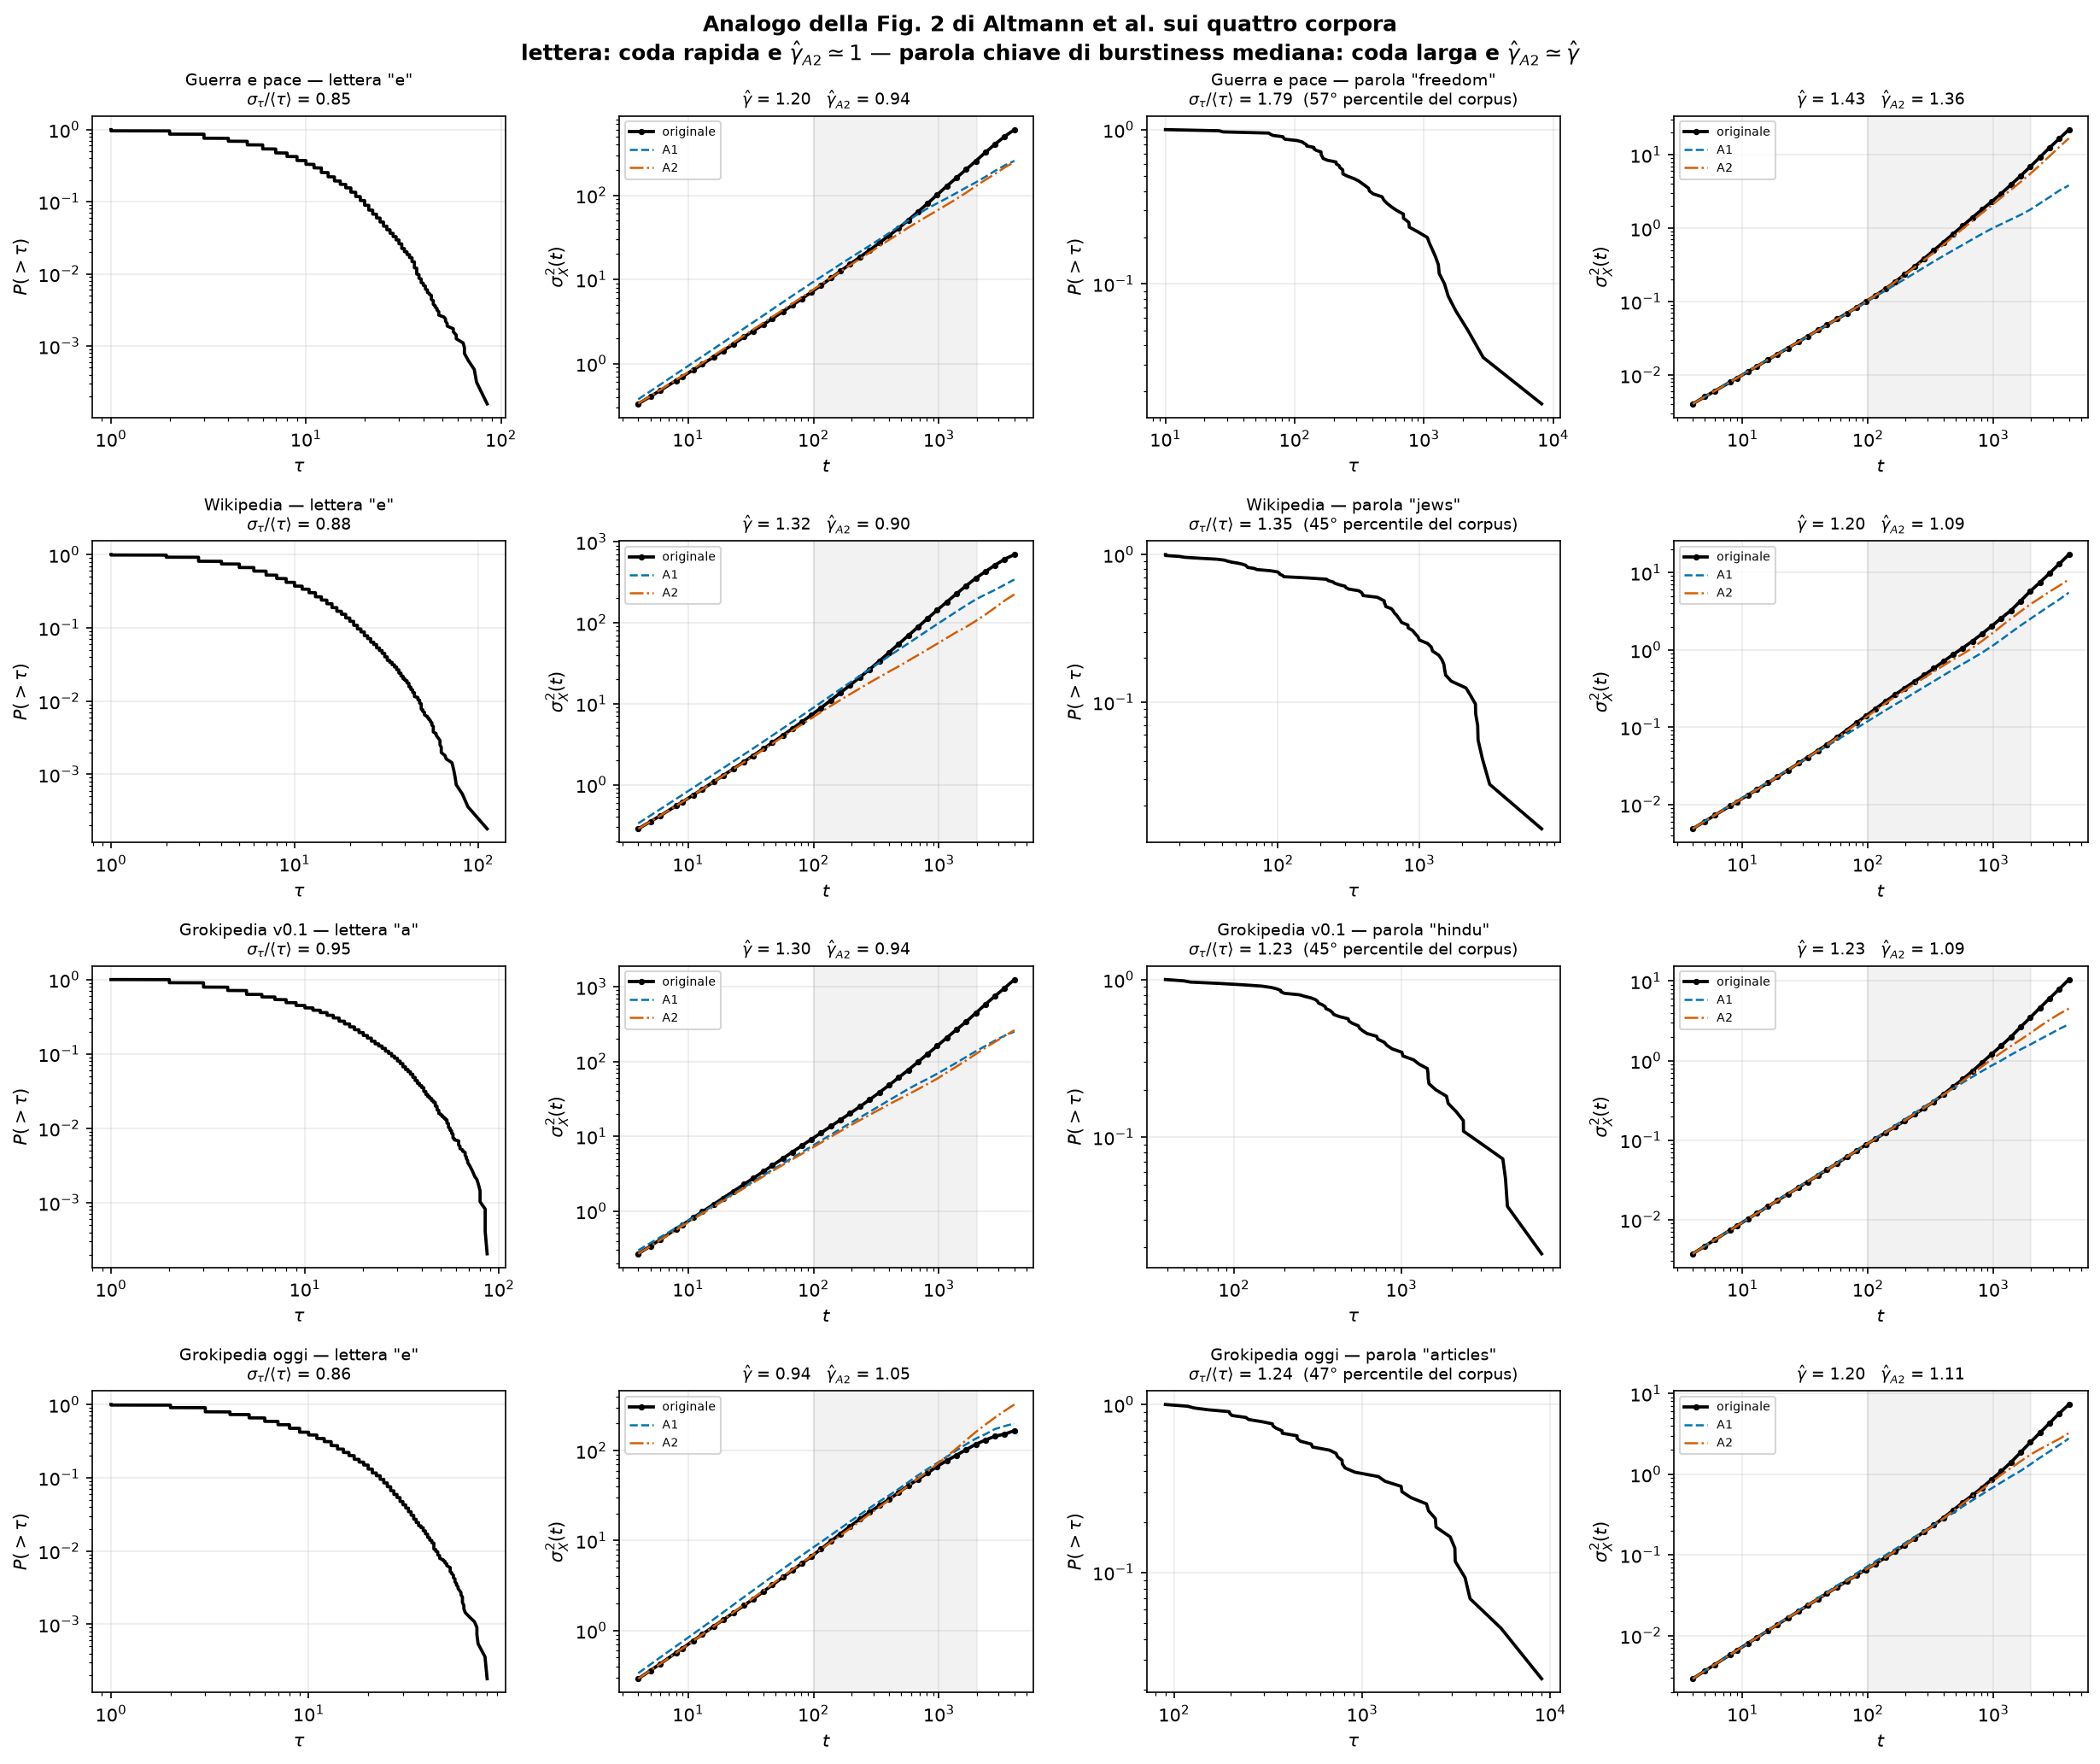
\includegraphics[width=\textwidth]{figure/cap5_altmann_fig2.png}
  \caption{Analogo della Figura~2 di~\cite{altmann2012} sui quattro corpora. Una
  riga per corpus; a sinistra la lettera più frequente del documento, a destra
  la parola chiave di burstiness mediana del corpus fra quelle con almeno
  \num{40} occorrenze, con il suo percentile indicato sopra il pannello. Per
  ciascuna, la distribuzione cumulata degli intervalli $P(>\tau)$ e la crescita
  della varianza del conteggio $\sigma_X^2(t)$, con le curve dei due null model
  del §\ref{sec:null} e la finestra di fit ombreggiata. La lettera ha coda
  rapida e $\hat\gamma_{A2} \simeq 1$; la parola di contenuto ha coda larga e
  $\hat\gamma_{A2}$ prossimo a $\hat\gamma$.}
  \label{fig:altmann-fig2}
\end{figure}

\paragraph{Il soggetto della voce non è una parola di contenuto.}
La parola chiave più ricorrente di un articolo enciclopedico, quella che il
criterio scartato sopra avrebbe selezionato, si comporta in modo opposto a
quello che il §\ref{sec:origini} prevede per il suo livello linguistico. Nella
voce \emph{Alexander the Great} di Wikipedia la parola \emph{alexander} ha
$\sigma_\tau/\langle\tau\rangle = 0.78$; in \emph{Sigmund Freud} di Grokipedia
\emph{freud} ha $0.72$. Sono valori sotto il limite poissoniano, cioè
distribuzioni \emph{più regolari del caso}, mentre la lettera \emph{e} negli
stessi testi dà $0.84$. Il confronto con la lettera non va però fatto sul valore
grezzo. Per un processo casuale in tempo discreto
$\sigma_\tau/\langle\tau\rangle$ non vale esattamente uno, ma tanto meno quanto
più corti sono gli intervalli: il null model A1, applicato alla stessa frequenza
della sequenza osservata, restituisce $0.95$ per la lettera \emph{e}, che ricorre
ogni dieci caratteri, e $1.00$ per una parola chiave, che ricorre ogni
duecento.

\paragraph{Il riferimento casuale dipende dalla frequenza.}
La ragione di quel $0.95$ è che gli intervalli sono numeri interi positivi. Se
le occorrenze sono collocate a caso con probabilità $f$ per carattere, la
distanza fra due consecutive è geometrica, e per la geometrica si ha
$\sigma_\tau/\langle\tau\rangle = \sqrt{1-f}$: il valore tende a uno solo nel
limite di eventi rari. Con $f = 1/10$, la frequenza della lettera \emph{e}, si
ottiene $0.949$; con $f = 1/200$, la frequenza tipica di una parola chiave,
$0.997$. Il valore poissoniano di riferimento non è dunque lo stesso ai due
livelli, ed è più basso proprio dove gli eventi sono più fitti. Confrontare
\emph{alexander} e la lettera \emph{e} sui valori grezzi significherebbe
attribuire alla struttura del testo una differenza che è invece un effetto
della sola frequenza.

Rapportando ciascuna misura al proprio valore casuale l'effetto si toglie, e
resta $0.78$ per \emph{alexander} contro $0.88$ per la lettera: il soggetto
della voce è più regolare di una lettera anche dopo aver tolto l'effetto della
frequenza, e la differenza fra i due, lungi dall'essere prodotta dalla
normalizzazione, ne esce accentuata.

\paragraph{Perché il soggetto si comporta così.}
La ragione è che in prosa enciclopedica il soggetto non è un tema fra altri,
che alterna presenza e assenza lungo il testo, ma il tema unico: compare come soggetto grammaticale di quasi ogni
periodo, e i suoi intervalli ereditano allora la statistica della lunghezza
delle frasi anziché quella dell'alternanza tematica. La verifica è diretta.
Nei sei articoli esaminati il soggetto ricorre una volta ogni $1.4$--$1.7$
frasi, con lo stesso valore in Wikipedia e in Grokipedia. I suoi intervalli sono
quindi lunghezze di frase, e ne ereditano la variabilità: le
lunghezze di frase di quegli articoli hanno
$\sigma_\tau/\langle\tau\rangle$ fra $0.33$ e $0.73$, e il soggetto della voce
si colloca poco sopra, fra $0.54$ e $0.78$, comunque sotto l'unità che
segnerebbe l'assenza di struttura. Per confronto, \emph{natásha} in un segmento
di \emph{Guerra e pace} ricorre una volta ogni $5.1$ frasi e ha
$\sigma_\tau/\langle\tau\rangle = 3.24$: lì la ricorrenza non segue il ritmo del
periodo ma l'alternanza delle scene.

Il soggetto della voce funziona quindi da marcatore sintattico e non semantico,
e la sua ricorrenza è governata dal ritmo del periodo, non dalla persistenza di
un argomento. Non è un difetto della misura ma un tratto del genere
enciclopedico, e va tenuto presente nel confrontare la burstiness lessicale fra
generi diversi: è la ragione per cui la parola mostrata nella
Figura~\ref{fig:altmann-fig2} viene scelta sulla mediana e non sul massimo.

% ---------------------------------------------------------------------
\section{Il divario si apre al livello lessicale}
\label{sec:appaiato}

L'appaiamento per titolo permette un test più stringente del confronto fra
medie. Confrontare la media di Wikipedia con quella di Grokipedia lascia
aperta l'obiezione che le due medie siano calcolate su argomenti diversi, e
che la differenza rifletta il contenuto anziché la scrittura. Il test appaiato
la chiude: per ciascuna delle \num{39} voci, che nei due corpora tratta lo
stesso argomento, si calcola la differenza fra il valore di Grokipedia e
quello di Wikipedia, e si verifica con il test dei ranghi segnati di Wilcoxon
che la mediana di quelle \num{39} differenze sia diversa da zero. Il test è
non parametrico, quindi non assume che le differenze siano distribuite
normalmente, assunzione che con \num{39} osservazioni e distribuzioni
asimmetriche non sarebbe difendibile.

Il test dà, per la versione attuale di Grokipedia,
$-0.167$ sulle parole chiave e $-0.010$ sulle lettere; ai due livelli intermedi
le differenze valgono $-0.037$ per le parole funzione e $-0.157$ per i controlli
appaiati, tutte con significatività inferiore a $10^{-2}$. La versione v0.1 dà
$-0.012$, $-0.039$, $-0.116$ e $-0.133$.

I quattro numeri vanno letti come una scala. Alle lettere Grokipedia e
Wikipedia distano un centesimo di unità di burstiness, cioè circa l'uno per
cento del valore misurato: a quel livello i due corpora sono, in pratica, lo
stesso testo. Alle parole funzione la distanza quadruplica, ma resta piccola in
termini relativi. Ai due livelli lessicali passa a circa sedici centesimi, oltre
un decimo del valore misurato e più di un ordine di grandezza sopra il livello
delle lettere.

La scala ha però un solo gradino, non tre. La differenza fra i livelli
sub-lessicali e quelli lessicali è netta; quella fra i due livelli lessicali non
esiste: $-0.157$ sui controlli a frequenza appaiata contro $-0.167$ sulle parole
chiave sono lo stesso numero. Il testo generato non perde dunque le parole di
contenuto più di quanto perda le altre parole della stessa frequenza. Ciò che i
dati sostengono è che riproduca le regolarità dei livelli bassi e abbassi
uniformemente la burstiness a livello di parola, non che perda selettivamente la
persistenza tematica.

\paragraph{Il divario alla lunghezza di controllo.}
\label{sec:robustezza-neff}
L'intera catena è stata ripetuta a $N_{\mathrm{eff}} = \num{80000}$ caratteri,
lunghezza a cui sopravvivono \num{35} delle \num{39} terne; per isolare
l'effetto della finestra, i valori a \num{60000} sono ricalcolati sulle stesse
\num{35}. Alle lettere e alle parole funzione il divario appaiato è stabile, da
$-0.010$ a $-0.011$ e da $-0.037$ a $-0.045$; ai due livelli lessicali si separa
in direzioni opposte, con i controlli appaiati da $-0.164$ a $-0.195$ e le parole
chiave da $-0.167$ a $-0.130$, quest'ultima con significatività che scende a
$p = 0.027$. Alla lunghezza maggiore il divario sulle parole chiave è dunque
\emph{minore} di quello sui controlli appaiati. Ciò che risulta robusto è il
salto dal livello sub-lessicale a quello lessicale; l'ulteriore crescita fino
alle parole chiave non lo è. Anche l'esponente di coda è instabile fra le due
lunghezze, da $2.19$ a $2.50$ su Grokipedia e da $2.37$ a $2.25$ su Wikipedia,
coerentemente con l'avvertenza del §\ref{sec:coda-risultati}.

La Figura~\ref{fig:altmann-fig3} riporta le stesse sequenze nel piano che
\cite{altmann2012} usa per la propria Figura~3: la burstiness in ascissa e
l'esponente di correlazione in ordinata, un punto per sequenza, con un simbolo
diverso per livello linguistico. La gerarchia vi si legge come una disposizione
spaziale: le lettere, gli spazi e le vocali si addensano in una colonna stretta
attorno a $\sigma_\tau/\langle\tau\rangle \simeq 0.5$, le parole funzione e i
controlli appaiati occupano la regione centrale, le parole chiave si spingono a
destra e in alto. È la stessa gerarchia dei paragrafi precedenti, vista tutta
insieme invece che un livello alla volta.

Il piano rende però visibile anche una proprietà che i confronti per livello
non mostrano, e che è l'osservazione centrale di quel lavoro: l'angolo in
basso a destra è vuoto. Non esistono, cioè, sequenze molto \emph{bursty} e
insieme poco correlate. Sui quattro corpora di questa tesi la regolarità si
quantifica così: delle $451$ sequenze con $\sigma_\tau/\langle\tau\rangle >
1.5$, soltanto $17$, il $3.8\%$, hanno $\hat\gamma < 1.1$, e fra quelle con
burstiness superiore a $2$ l'esponente non scende mai sotto $1.05$. L'angolo
opposto, invece, è popolato: delle $3500$ sequenze sotto il valore poissoniano
$\sigma_\tau/\langle\tau\rangle = 1$, il $15.9\%$ ha $\hat\gamma > 1.2$.

L'asimmetria fra i due angoli è la firma di una relazione a senso unico. La
burstiness produce correlazione, come mostra la~\eqref{eq:eq4}, e una sequenza
con vuoti lunghi non può quindi risultare scorrelata; il viceversa non vale,
perché la correlazione può venire anche dall'ordine degli intervalli e
manifestarsi senza alcuna coda pesante. La correlazione di rango fra le due
quantità è positiva e significativa in tutti e quattro i corpora, da $+0.22$ su
Wikipedia a $+0.36$ sul romanzo. Il meccanismo descritto in~\cite{altmann2012}
sui romanzi si ritrova dunque identico nella prosa enciclopedica e in quella
generata, ed è un risultato indipendente dal divario misurato sopra: riguarda
come le due grandezze si legano fra loro, non quanto valgano.

\begin{figure}[htbp]
  \centering
  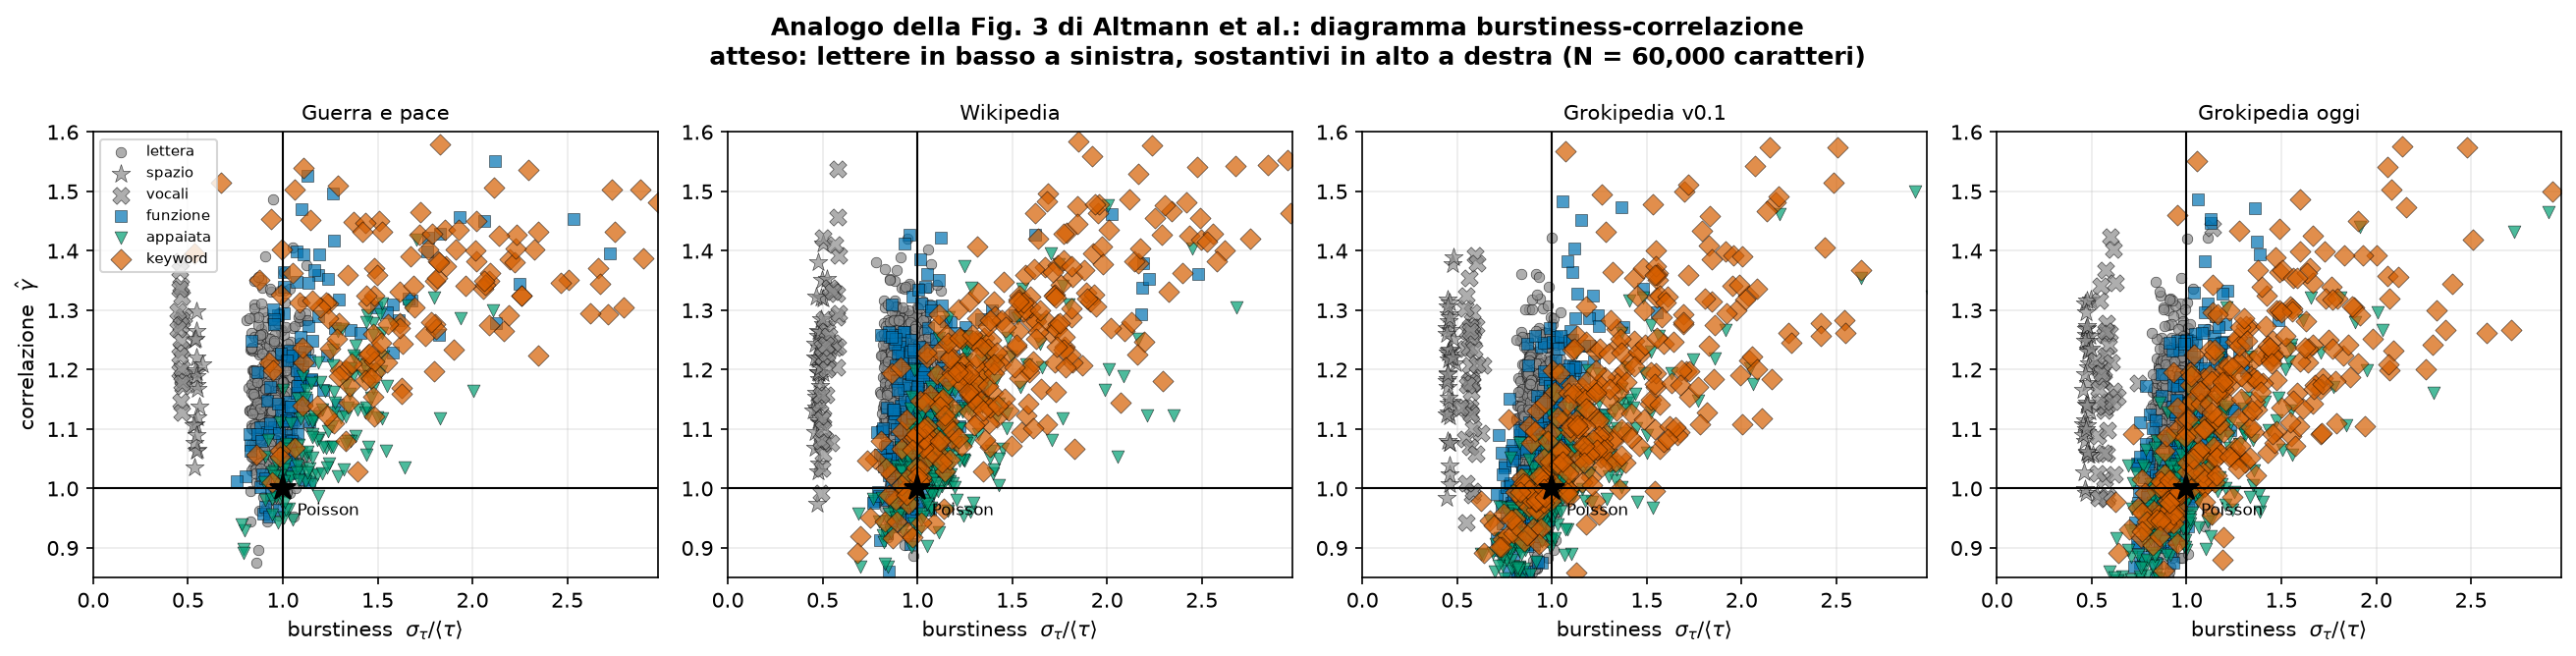
\includegraphics[width=\textwidth]{figure/cap5_altmann_fig3.png}
  \caption{Analogo della Figura~3 di~\cite{altmann2012}: diagramma
  burstiness--correlazione sui quattro corpora, un punto per sequenza. Oltre ai
  quattro livelli usati nel resto del capitolo sono riportati i due livelli
  sub-lessicali tenuti come diagnostica, gli spazi e le vocali. Le linee nere
  segnano il processo di Poisson,
  $\sigma_\tau/\langle\tau\rangle = 1$ e $\hat\gamma = 1$. L'angolo in basso a
  destra è praticamente vuoto in tutti e quattro i corpora: sequenze molto
  bursty e insieme poco correlate non si osservano.}
  \label{fig:altmann-fig3}
\end{figure}

\paragraph{I due quadranti che restano.} La lettura del piano fatta finora
riguarda la diagonale: l'angolo in basso a destra vuoto e quello in alto a
sinistra popolato. Gli altri due separano però i corpora meglio di qualunque
media, e la Figura~\ref{fig:quadranti} li riporta separatamente. Fra le parole
chiave, l'angolo in alto a destra è la posizione canonica
di~\cite{altmann2012}, quella in cui la sequenza è insieme bursty e correlata.
Vi ricade il $91.4\%$ delle sequenze di \emph{Guerra e pace} e l'$87.5\%$ di
quelle di Wikipedia, ma solo il $74.0\%$ di Grokipedia v0.1 e il $77.3\%$
della versione attuale. La differenza finisce quasi interamente nell'angolo
opposto, in basso a sinistra, dove la parola è più regolare di un processo di
Poisson e insieme priva di correlazione a lungo raggio: $0\%$ sul romanzo,
$5.1\%$ su Wikipedia, $15.4\%$ su Grokipedia v0.1 e $14.3\%$ sulla versione
attuale. Una parola chiave generata su sette si trova dunque nell'angolo
opposto a quello canonico, contro una su venti in Wikipedia. Il test appaiato
sulle \num{39} voci conferma che non è un effetto di composizione del
campione: la quota di parole chiave in basso a sinistra cresce in $21$ e $22$
voci su $39$, con differenza mediana $+0.143$ e $p < 10^{-3}$ per entrambe le
versioni.

Due controlli escludono le spiegazioni strumentali. Il null model A1
restituisce $\hat\gamma = 0.983$ in tutti e quattro i corpora, identico alla
terza cifra, quindi la soglia $\hat\gamma = 1$ non è tarata diversamente da un
corpus all'altro; il valore calibrato non è però esattamente uno, cosicché la
soglia è lievemente generosa verso il lato correlato, allo stesso modo per
tutti. E la quota di parole in basso a sinistra resta più alta in Grokipedia
dentro quattro fasce di frequenza su cinque, da $0.159$ contro $0.050$ per le
parole con $26$--$35$ occorrenze a $0.303$ contro $0.076$ per quelle con più di
$80$. Fa eccezione la fascia più bassa, $15$--$25$ occorrenze, dove il rapporto
si inverte, $0.065$ contro $0.200$; lì però le parole chiave di Wikipedia sono
dieci in tutto e la quota è stimata su di esse. Il divario non dipende quindi
dal fatto che le parole chiave di Wikipedia siano più frequenti, salvo nella
fascia in cui il confronto ha meno appoggio.

Guardare dentro il quadrante non rivela più un gruppo omogeneo. Separando le
parole che compaiono nel titolo della voce dalle altre, le $14$ di Wikipedia si
dividono a metà, e le $39$ di Grokipedia si dividono in $18$ soggetti di voce e
$21$ altre parole, prevalentemente aggettivi generici: \emph{economic} in cinque
voci, \emph{military} in tre, \emph{urban} in due. Sono concentrazioni modeste,
e soprattutto non sono più quelle che la lista di parole funzione originaria
lasciava passare: con quella lista, il quadrante conteneva \emph{like} in dodici
voci, \emph{amid} in nove e \emph{including} in sei, cioè i connettivi che
costituiscono il vizio stilistico più evidente del testo generato. Quei termini
sono ora classificati come parole funzione, che è ciò che sono, e il
§\ref{sec:effetto-stoplist} misura quanto la loro presenza fra le parole chiave
alterasse i risultati.

\begin{figure}[htbp]
  \centering
  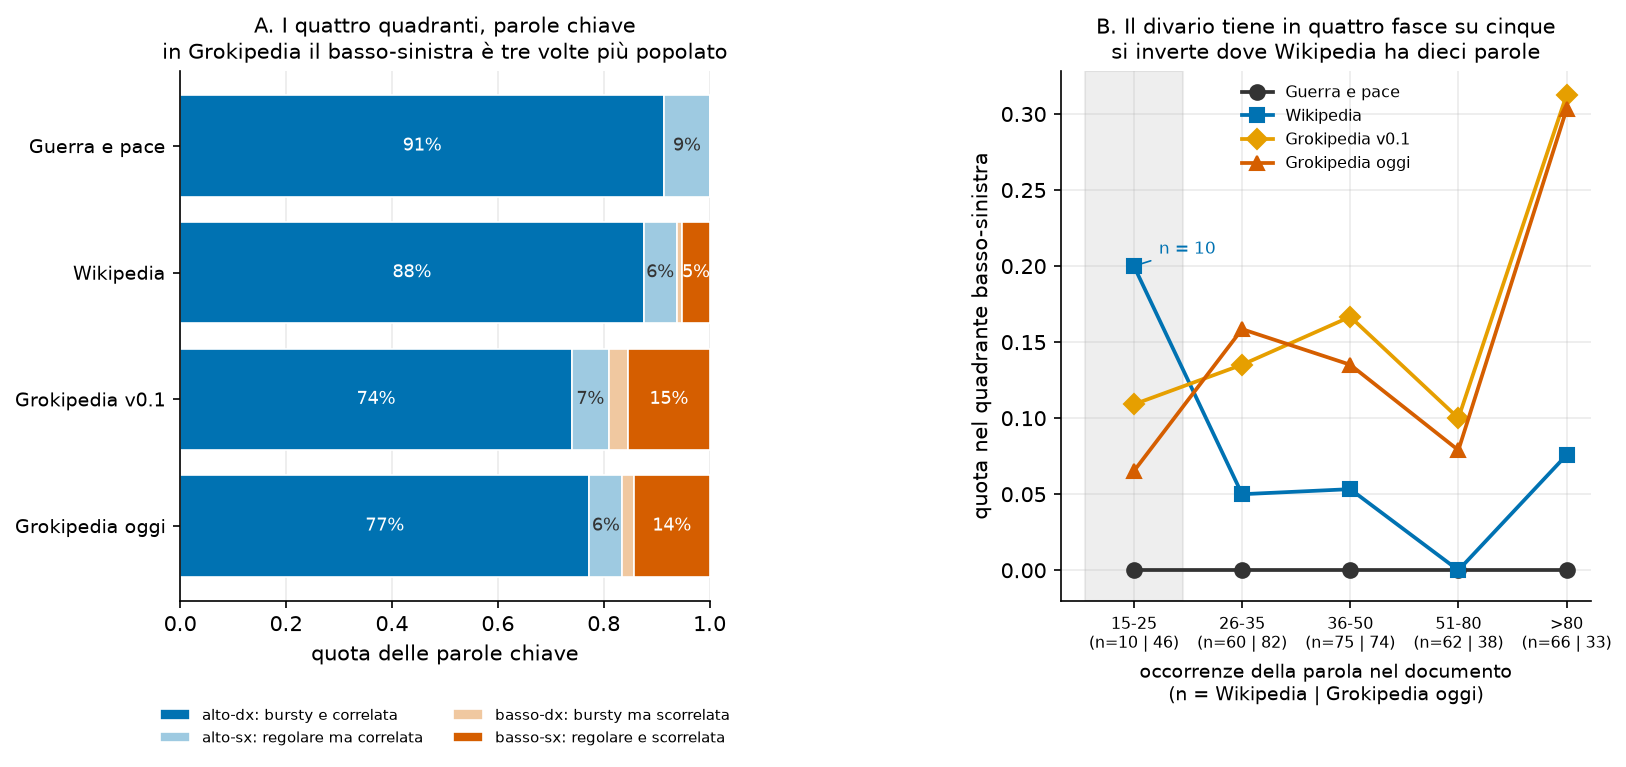
\includegraphics[width=\textwidth]{figure/cap5_quadranti.png}
  \caption{Lettura per quadranti del piano della
  Figura~\ref{fig:altmann-fig3}, sulle sole parole chiave. A: composizione per
  quadrante, un corpus per riga; le quote sotto il $5\%$ non sono etichettate. B:
  quota di parole chiave nel quadrante in basso a sinistra, separando le parole
  per numero di occorrenze nel documento; sotto ciascuna fascia è indicato
  quante parole chiave vi cadono in Wikipedia e in Grokipedia. Il divario tiene
  in quattro fasce su cinque e si inverte nella più bassa, dove Wikipedia ne ha
  dieci in tutto e la fascia è ombreggiata per segnalarlo.}
  \label{fig:quadranti}
\end{figure}

\paragraph{Un effetto di scala da neutralizzare.} Le voci di Grokipedia hanno
frasi sensibilmente
più lunghe di quelle di Wikipedia: $4.38$ frasi ogni mille caratteri contro
$6.92$. Poiché in questo capitolo il tempo è contato in caratteri, la scala
degli intervalli $\tau$ non è la stessa nei due corpora, e un testo con frasi
più lunghe tende ad avere intervalli più lunghi anche a parità di struttura
tematica. Il coefficiente di variazione è un rapporto e non risente di una
dilatazione uniforme dell'asse, ma la dilatazione qui non è uniforme, perché
agisce solo sui livelli definiti su unità linguistiche. Il
§\ref{sec:entropia-intervalli} introduce la misura che elimina il problema;
fino a quel punto il divario va considerato provvisorio.

Il riferimento letterario, infine, non è appaiato per argomento con nessuno dei
tre corpora enciclopedici: entra nei confronti come livello medio e non nei test
appaiati.

% ---------------------------------------------------------------------
\section{Quale meccanismo genera la correlazione}
\label{sec:decomposizione}

Sapere che un testo ha correlazioni a lungo raggio non dice da dove esse
vengano. Il §\ref{sec:null} ha introdotto i due null model che separano le due
origini possibili e la quota di burstiness $q$ della~\eqref{eq:quota}, che vale
circa uno quando la correlazione è interamente spiegata dalla distribuzione
degli intervalli, e circa zero quando è invece l'ordine in cui le occorrenze si
susseguono a produrla.

Il primo pannello della Figura~\ref{fig:decomposizione} riporta $q$ ai quattro
livelli. Sulle lettere il valore è negativo in tutti e quattro i corpora, da
$-0.06$ su Wikipedia a $-0.19$ su Grokipedia v0.1: le lettere sono correlate,
come mostra il $\hat\gamma$ maggiore di uno, ma non sono \emph{bursty}, e la
correlazione viene interamente dall'ordine. Sulle parole chiave il valore sale a
$0.89$ sul romanzo, $0.77$ su Wikipedia, $0.70$ sulla v0.1 e $0.74$ sulla
versione attuale di Grokipedia: qui quasi tutta la correlazione è già contenuta nella
distribuzione degli intervalli. I due livelli intermedi interpolano fra i due
regimi in modo ordinato.

La dissociazione fra il livello dei caratteri e quello del contenuto, che
in~\cite{altmann2012} è osservata su romanzi, si ritrova quindi identica nella
prosa enciclopedica e anche nella prosa generata. Il secondo pannello mostra la
stessa cosa in termini di esponenti: le curve piene sono $\hat\gamma$ e quelle
tratteggiate $\hat\gamma_{A2}$, e la distanza verticale fra le due è il
contributo dell'ordine delle occorrenze. Sulle lettere le due curve sono
separate e la tratteggiata sta all'unità; sulle parole chiave si avvicinano e
salgono insieme.

I valori dei tre corpora enciclopedici sono però troppo vicini perché la
differenza sia interpretabile: fra Wikipedia e Grokipedia vale $0.03$ alla
lunghezza di lavoro e cambia segno a quella di controllo del
§\ref{sec:robustezza-neff}. I dati non consentono quindi di attribuire ai due
corpora un'origine diversa della correlazione, ma soltanto un'intensità diversa.

Sulla riga dei controlli appaiati per Grokipedia, infine, la quota è stimabile
solo su $6$ documenti su $39$ per la versione v0.1 e su $8$ per quella
attuale. La ragione non è un difetto della stima ma la grandezza stessa: $q$
ha $\hat\gamma - 1$ al denominatore, e viene calcolata soltanto dove quel
denominatore supera $0.05$, perché sotto quella soglia il rapporto è dominato
dall'errore. A quel livello i documenti di Grokipedia hanno $\hat\gamma$
mediano pari a $1.003$ per la v0.1 e $1.015$ per la versione attuale, contro
$1.091$ di Wikipedia: le loro sequenze di controllo sono essenzialmente
scorrelate, e non c'è alcuna correlazione da decomporre nelle due origini.
L'esclusione è quindi essa stessa un dato, perché è il livello in cui il testo
generato si avvicina di più al caso, ma il valore di $q$ che sopravvive sui
pochi documenti restanti riguarda proprio quelli in cui una correlazione c'è,
e non va letto come una misura del corpus.

\begin{figure}[htbp]
  \centering
  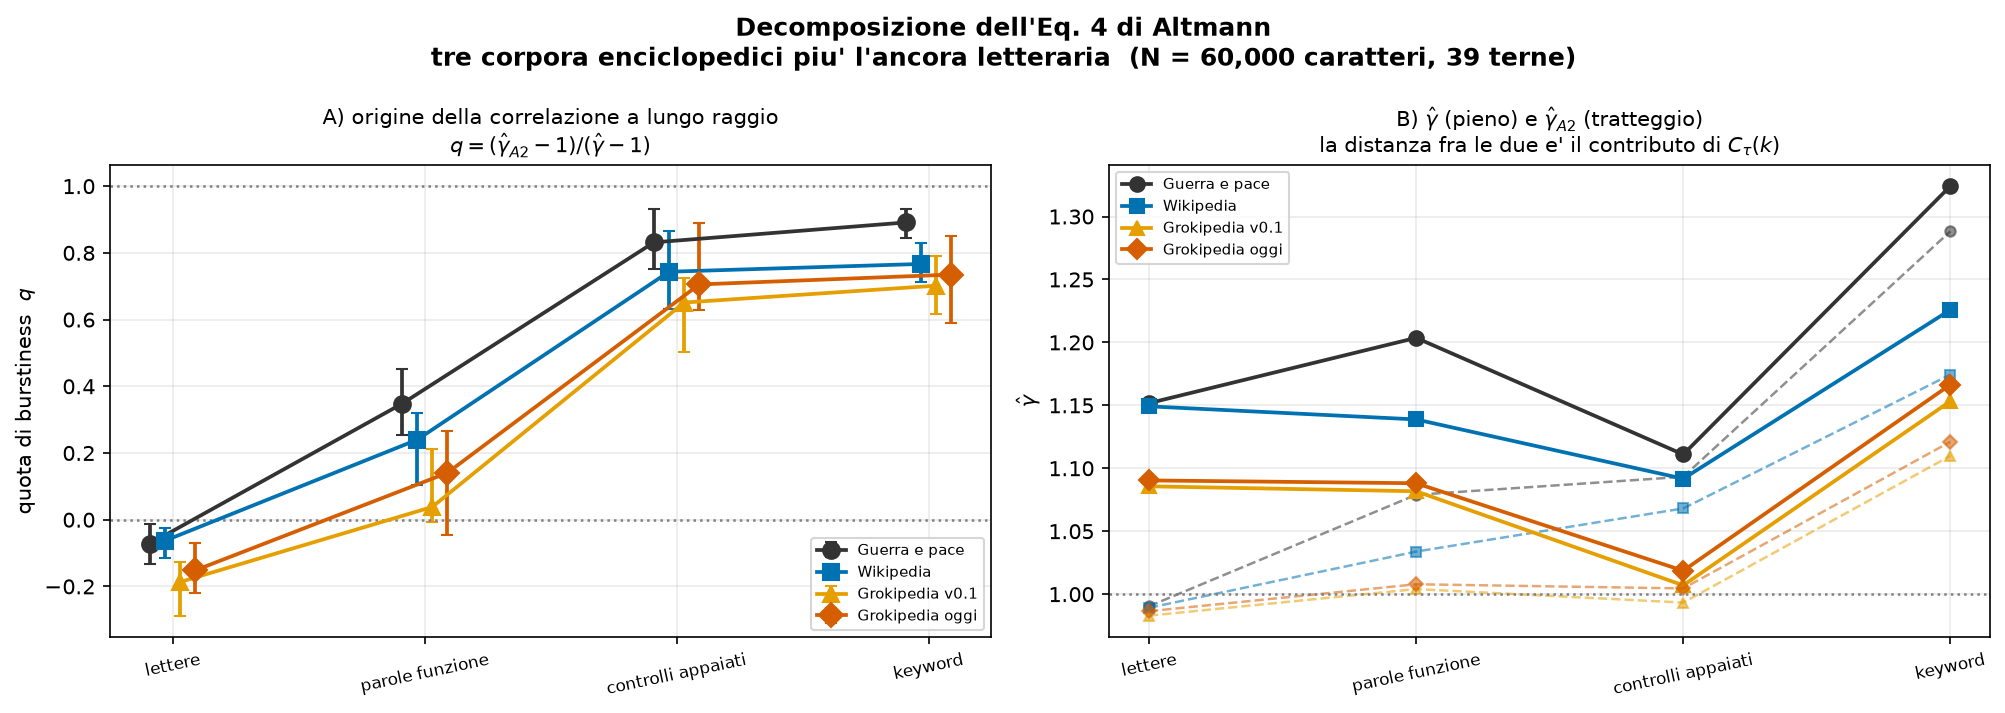
\includegraphics[width=\textwidth]{figure/cap5_decomposizione_eq4.png}
  \caption{Decomposizione della correlazione nelle sue due origini. A: quota
  $q$ della~\eqref{eq:quota} ai quattro livelli linguistici, con intervalli di
  confidenza; $q \simeq 0$ indica correlazione dovuta all'ordine delle
  occorrenze, $q \simeq 1$ correlazione dovuta alla distribuzione degli
  intervalli. B: esponente $\hat\gamma$ (linea piena) e $\hat\gamma_{A2}$
  (tratteggiata) agli stessi livelli; la distanza fra le due curve è il
  contributo della correlazione fra intervalli successivi.}
  \label{fig:decomposizione}
\end{figure}

% ---------------------------------------------------------------------
\section{La coda della distribuzione degli intervalli}
\label{sec:coda-risultati}

Il §\ref{sec:coda} ha osservato che la relazione fra esponente di coda e
esponente di correlazione, nella forma in cui compare in~\cite{altmann2012},
presuppone una distribuzione degli intervalli di cui la coda non viene misurata
ma assunta. Qui la coda viene stimata direttamente, adottando il modello
troncato
\begin{equation}
  p(\tau) \;\sim\; \tau^{-\mu}\,e^{-\tau/\tau_c}
  \label{eq:coda-troncata}
\end{equation}
e determinando $\mu$ e $\tau_c$ per massima verosimiglianza, con intervalli di
confidenza di profilo.

L'analisi della coda comprende, oltre ai quattro livelli usati nel resto del
capitolo, due livelli sub-lessicali aggiuntivi tenuti come diagnostica, le
vocali e gli spazi, per un totale di ventiquattro celle. Il primo risultato
riguarda la forma stessa della distribuzione: il confronto di verosimiglianza
fra la~\eqref{eq:coda-troncata} e una legge di potenza pura rifiuta
quest'ultima in tutte e ventiquattro, con significatività numericamente
indistinguibile da zero. La coda esiste, ma è tagliata.

Il primo pannello della Figura~\ref{fig:coda} riporta $\mu$ ai quattro livelli.
La banda verde segna la regione $2 < \mu < 3$ entro cui la~\eqref{eq:eq8} è
derivata assumendo una legge di potenza pura. Che le stime vi cadano dentro o
fuori non dice nulla sulla convergenza dei momenti: nella
~\eqref{eq:coda-troncata} il taglio li rende finiti per qualunque $\mu$, e il
rifiuto della potenza pura in tutte e ventiquattro le celle toglie il
presupposto sotto cui la banda avrebbe quel significato. Resta un riferimento
utile perché è la regione in cui il paper colloca il proprio valore assunto.
I simboli grigi segnalano le celle in cui il fit degenera in un
esponenziale puro e $\mu$ non è interpretabile, e le linee di collegamento le
saltano. Sono sette celle su sedici: tutti e quattro i corpora sul livello delle
lettere, e i tre corpora enciclopedici su quello delle parole funzione.

Alle parole funzione il romanzo è l'unico dei quattro il cui fit non degenera,
con $\tau_c = 5.3$ contro $1.7$--$1.9$: le sue parole funzione conservano un
tratto di coda a legge di potenza che negli altri tre corpora non esiste, e a
quel livello il coefficiente di variazione dà lo stesso quadro, $1.19$ contro
valori fra $0.97$ e $1.03$ indistinguibili da un processo di Poisson.

Sarebbe naturale leggerlo come una differenza di genere, e il controllo non lo
conferma. Ripetendo la stessa procedura sui tre romanzi inglesi impiegati come
controllo in questo capitolo, il fit sulle parole funzione degenera su
\emph{Moby Dick} ($\tau_c = 1.7$, esattamente il valore dei corpora
enciclopedici) e su \emph{David Copperfield} ($\tau_c = 2.8$), e sopravvive per
poco su \emph{Middlemarch} ($\tau_c = 3.2$); il coefficiente di variazione dà
$1.03$, $1.09$ e $1.08$, cioè valori compresi fra Wikipedia e
\emph{Guerra e pace} e nel primo caso identici a quelli enciclopedici. A questo
livello l'eccezione è quindi del testo e non del genere, come il
§\ref{sec:tre-corpora} osserva anche sul livello delle parole chiave. Il confronto fra i quattro
corpora resta perciò leggibile soltanto sulle parole chiave, dove i valori
stanno fra $1.76$ e $2.37$; sui controlli appaiati tutti e quattro i fit sono al
limite della degenerazione e gli intervalli di confidenza superano l'unità di
ampiezza.

Il confronto con~\cite{altmann2012} chiude qui un cerchio. In quel lavoro $\mu$
non viene stimato ma assunto: per costruire il limite inferiore di $\hat\gamma$
della propria Figura~3 gli autori adottano il valore $\mu = 2.4$. La stima
diretta condotta qui lo colloca dentro l'intervallo di confidenza di tutti e tre
i corpora enciclopedici, e a tre centesimi dal valore centrale di Wikipedia. Il
parametro che quel lavoro doveva postulare risulta dunque misurabile, e il
valore postulato corretto. Il confronto è legittimo perché $\mu$ designa in
entrambi i casi la pendenza della coda nella regione in cui la legge di potenza
vale; ciò che cambia è che qui quella regione è delimitata da un $\tau_c$
stimato anziché estesa all'infinito, e il capoverso seguente misura quanto la
differenza di modello sposti il numero.

Il corpus letterario fa eccezione, con $\mu = 1.76$ e intervallo di confidenza
$[1.40, 2.08]$, e su questo servono due precisazioni, perché il valore cade
sotto la banda $2 < \mu < 3$ entro cui la~\eqref{eq:eq8} è derivata. La prima
è che non è una particolarità di \emph{Guerra e pace}: ripetendo l'intera
procedura su tre altri romanzi inglesi, segmentati e misurati allo stesso
modo, si ottiene $1.51$ su \emph{Moby Dick}, $2.10$ su \emph{Middlemarch} e
$1.96$ su \emph{David Copperfield}, tutti sotto il valore di Wikipedia a ogni
quantile di $x_{\min}$ dall'ottantesimo in su. È un tratto della prosa
letteraria, non del testo scelto, ed è lo stesso fatto che il coefficiente di
variazione registra come burstiness massima: coda più pesante significa
esponente più piccolo.

La seconda è che il valore dipende dal modello con cui lo si stima. Sotto il
modello troncato adottato qui la banda $2 < \mu < 3$ non ha ruolo, perché il
taglio rende media e varianza finite per qualunque $\mu$; sotto il modello a
potenza pura, che è quello di~\cite{altmann2012}, lo stimatore di massima
verosimiglianza sugli stessi dati dà $2.49$ per il corpus letterario, dentro la
banda e a nove centesimi dal valore assunto nel paper. I due numeri non sono in
conflitto: descrivono la stessa coda sotto ipotesi diverse, e la scelta fra le
due è decisa dal rapporto di verosimiglianza, che rifiuta la potenza pura. La
misura non contraddice dunque il valore postulato in quel lavoro; ne circoscrive
il modello.

\begin{figure}[htbp]
  \centering
  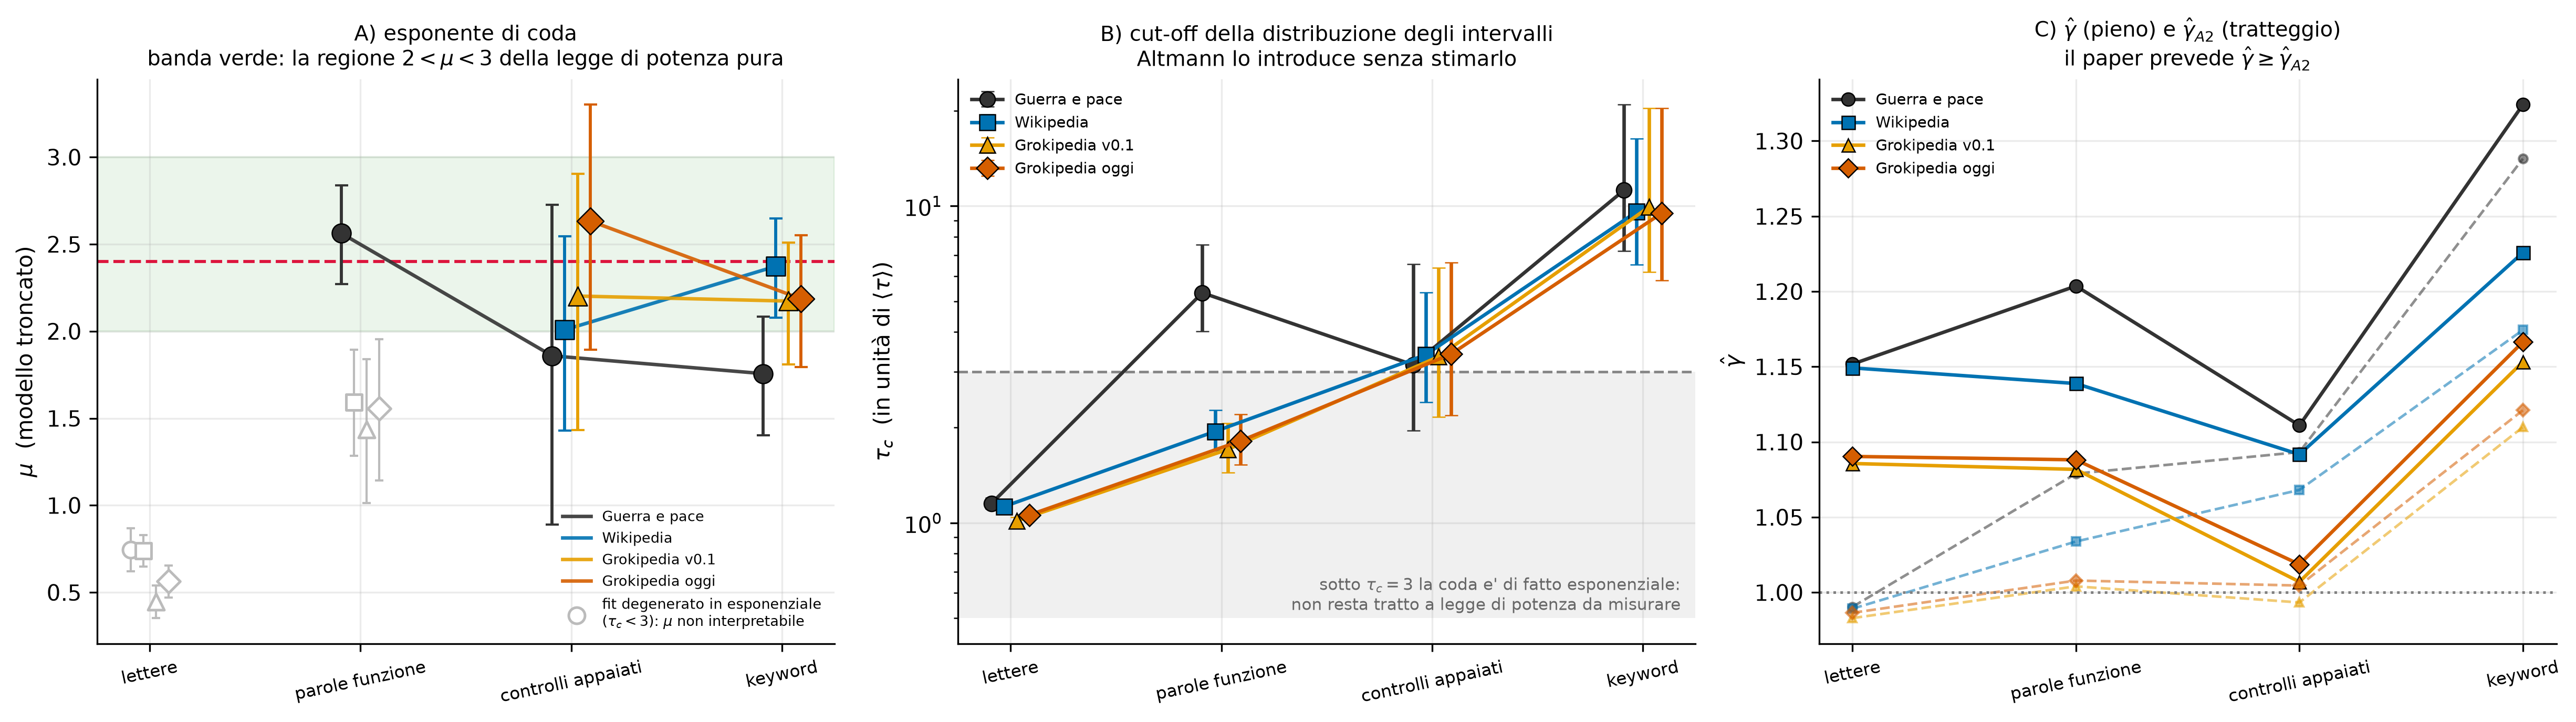
\includegraphics[width=\textwidth]{figure/cap5_esponente_coda.png}
  \caption{Stima diretta della coda della distribuzione degli intervalli. A:
  esponente $\mu$ della~\eqref{eq:coda-troncata} ai quattro livelli, con
  intervalli di confidenza di profilo; la banda verde è la regione $2<\mu<3$ in
  cui è derivata la~\eqref{eq:eq8} per la legge di potenza pura, mentre sotto il
  modello troncato adottato qui i momenti restano finiti per qualunque $\mu$ e
  la banda va letta come riferimento alla letteratura; i simboli grigi sono le
  celle in cui il fit degenera in un esponenziale e $\mu$ non è interpretabile,
  che le linee di collegamento saltano. B: cut-off
  $\tau_c$ agli stessi livelli, in unità dell'intervallo medio e con intervalli
  di confidenza di profilo; sotto la soglia tratteggiata non resta tratto a legge
  di potenza da misurare. C: $\hat\gamma$ (pieno) contro $\hat\gamma_{A2}$
  (tratteggiato) ai quattro livelli. La~\eqref{eq:disug1} è rispettata in tutte
  le celle: la curva piena sta sempre sopra la tratteggiata.}
  \label{fig:coda}
\end{figure}

\paragraph{Perché $\mu$ non serve a confrontare i corpora.}
I quattro valori non vanno però usati per ordinare i corpora, e la
Figura~\ref{fig:verosimiglianza} mostra perché: $\mu$ e $\tau_c$ sono
fortemente correlati, cosicché le regioni di confidenza congiunte sono creste
allungate anziché ellissi compatte e quelle dei tre corpora enciclopedici si
sovrappongono quasi interamente. A ciò si aggiunge la dipendenza dal punto in
cui si decide che la coda cominci: spostando $x_{\min}$ dal settantacinquesimo
al novantacinquesimo percentile $\mu$ passa da $1.65$ a $2.63$ su Wikipedia, una
variazione maggiore di ogni differenza fra corpora, e le curve si incrociano.

Di questa analisi non resta perciò un ordinamento fra corpora. Restano due
risultati, entrambi insensibili alla posizione esatta lungo la cresta: la legge
di potenza pura è rifiutata ovunque, e il cut-off cresce in modo ordinato
salendo nella gerarchia linguistica. Il cut-off è previsto
da~\cite{altmann2012} come conseguenza della discesa lungo quella stessa
gerarchia, e la sua esistenza è qui verificata invece che assunta.

\begin{figure}[htbp]
  \centering
  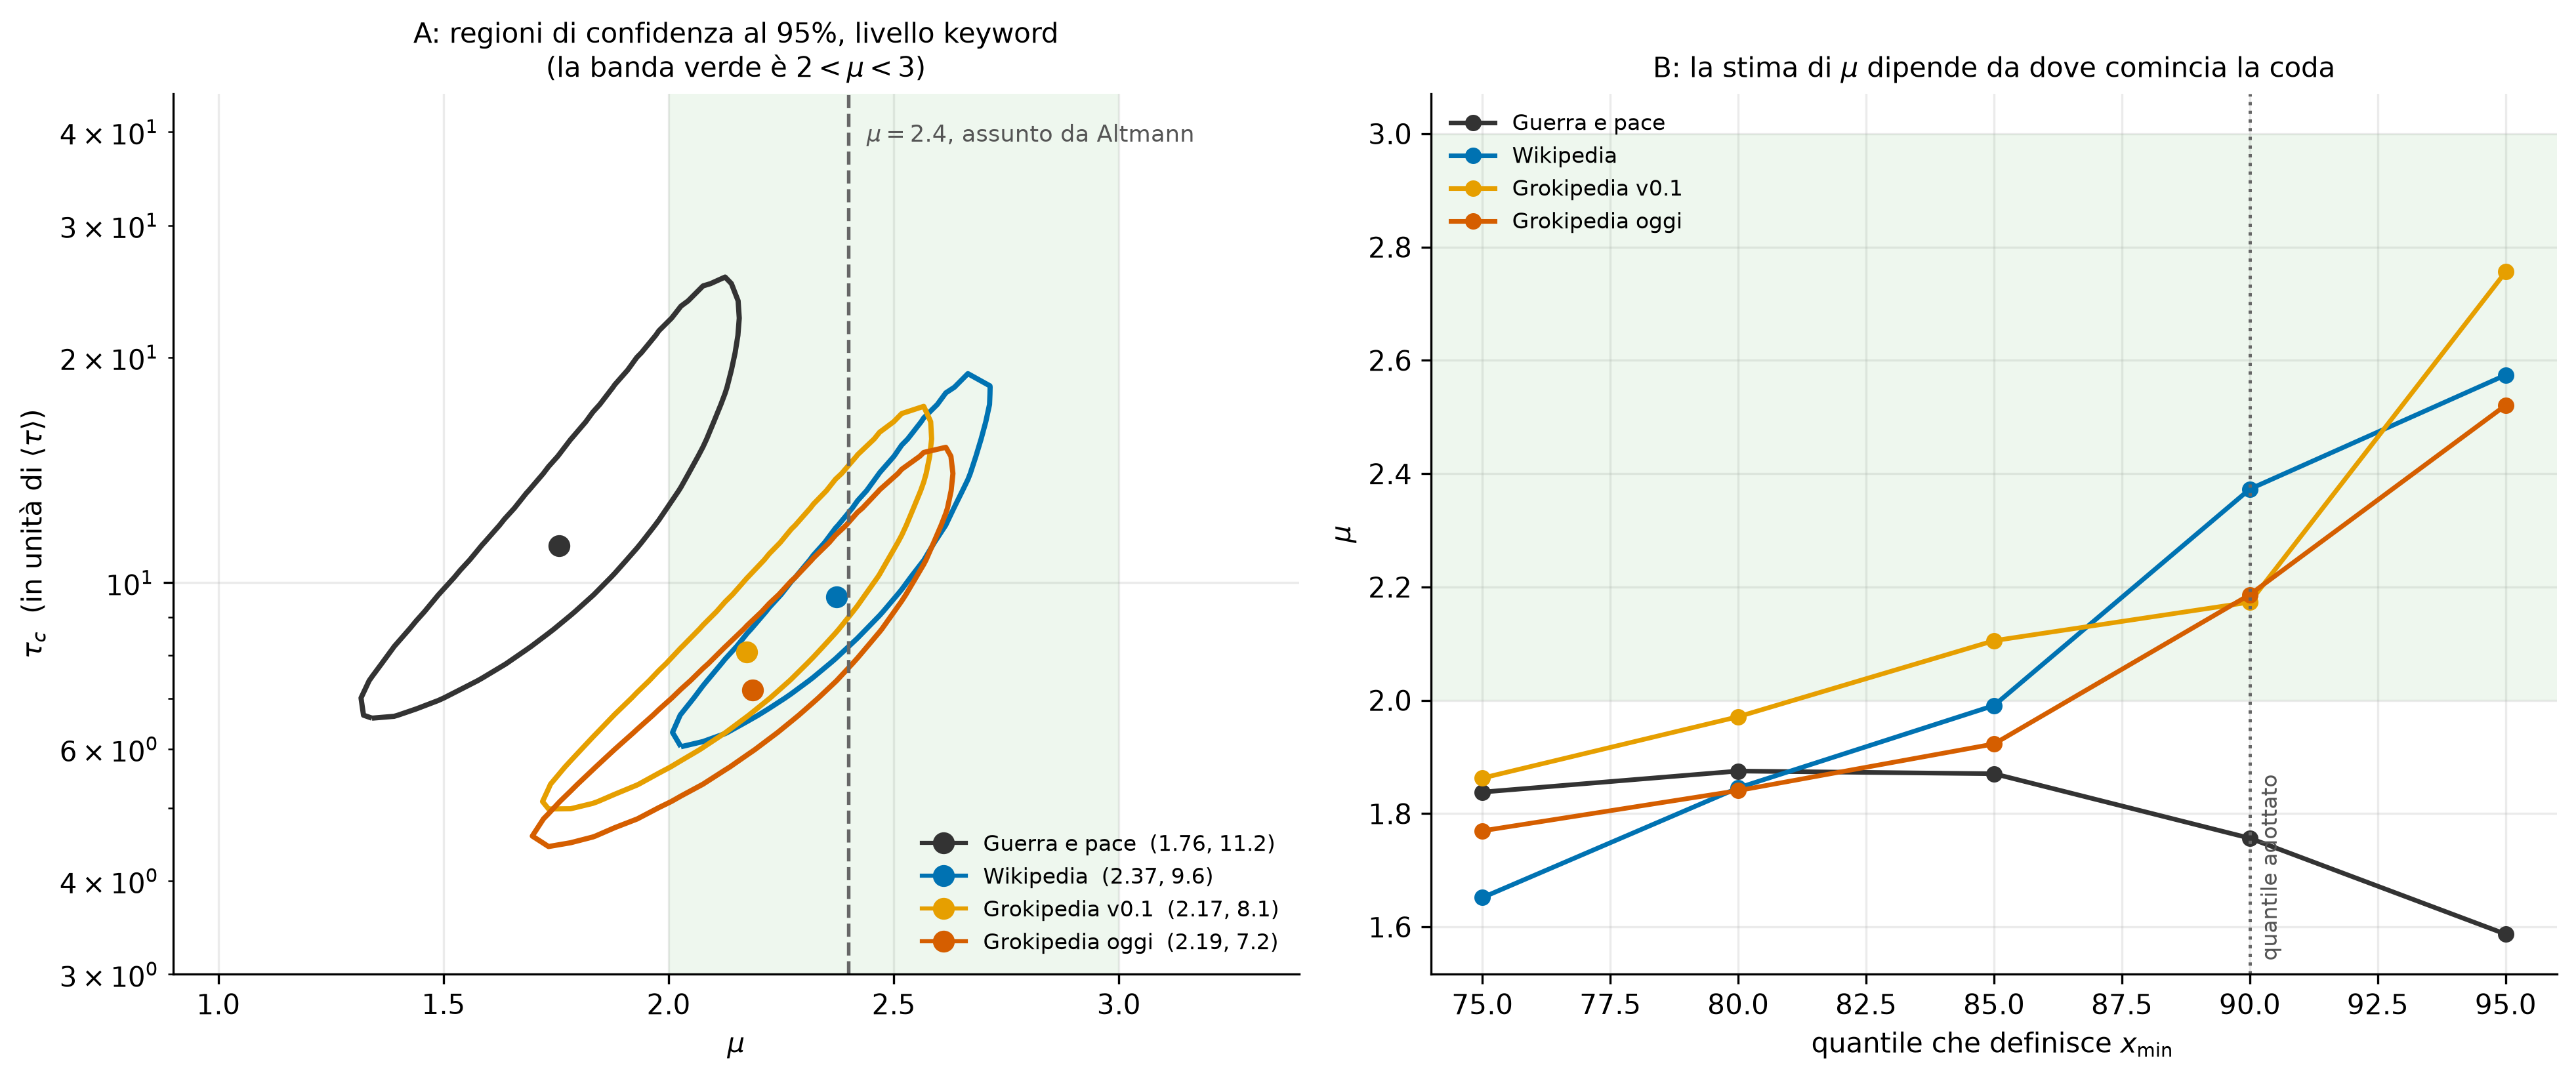
\includegraphics[width=\textwidth]{figure/cap5_verosimiglianza_coda.png}
  \caption{Perché l'esponente di coda non discrimina fra i corpora. A: regioni
  di confidenza congiunte al $95\%$ nel piano $(\mu, \tau_c)$ sul livello delle
  parole chiave, con $x_{\min}$ al novantesimo percentile; l'allungamento delle
  regioni è la correlazione fra i due parametri, e la linea tratteggiata è il
  valore $\mu = 2.4$ assunto in~\cite{altmann2012}. B: stima di $\mu$ al variare
  del quantile che definisce $x_{\min}$; le quattro curve si incrociano, cosicché
  l'ordinamento fra corpora dipende da quella scelta.}
  \label{fig:verosimiglianza}
\end{figure}

\paragraph{Il cut-off e la finestra di osservazione.} Il secondo pannello
della Figura~\ref{fig:coda} riporta $\tau_c$ ai quattro livelli, con
intervalli di confidenza di profilo. È l'altra metà di ciò
che~\cite{altmann2012} introduce senza stimare: il cut-off vi compare come
conseguenza necessaria della discesa nella gerarchia, ma non gli viene mai
assegnato un valore. Cresce in modo ordinato salendo nella gerarchia: circa
$1.1$ volte l'intervallo medio sulle lettere, dove la coda è di fatto già
esponenziale, $3.2$--$3.4$ sui controlli appaiati e $9.5$--$11.2$ sulle parole
chiave. La separazione fra i due livelli superiori è netta. Fra i quattro
corpora, invece, gli intervalli di confidenza si sovrappongono ampiamente:
neppure il cut-off ordina i corpora, e la sola cella in cui la separazione è
significativa è quella delle parole funzione del romanzo, discussa sopra.

Anche $\tau_c$ va poi letto come descrittore relativo alla lunghezza di analisi.
Ripetendo la stima sul romanzo a lunghezze crescenti, da \num{30000} a
\num{480000} caratteri, $\tau_c$ passa da $13.5$ a $94.7$: un fattore sette a
fronte di un fattore sedici sulla finestra, con un andamento non monotono che
scende prima di risalire. Il taglio non è dunque un puro artefatto, perché non
scala proporzionalmente alla finestra, ma non è nemmeno una lunghezza intrinseca
del testo. Sulla stessa serie $\mu$ si stabilizza attorno a $2.0$ alle finestre
maggiori, contro l'$1.76$ misurato alla lunghezza di lavoro: entrambi i
parametri descrivono la coda \emph{a quella lunghezza}, coerentemente con la
regola del §\ref{sec:lunghezza}.

\paragraph{Lo stimatore di Hill.} Dà sistematicamente valori più alti, $2.49$ sul
romanzo contro $1.76$ e circa $3.0$ sugli altri tre corpora contro
$2.2$--$2.4$, perché assume una legge di potenza pura su tutta la coda.
L'assenza di un plateau nel suo grafico diagnostico è ciò che ha motivato
l'adozione del modello troncato, e i suoi valori sono riportati solo a quel
titolo.

% ---------------------------------------------------------------------
\section{Entropia degli intervalli}
\label{sec:entropia-intervalli}

L'effetto di scala dichiarato nel §\ref{sec:appaiato} richiede una misura che
non risenta della lunghezza media delle frasi. È la ragione per cui il
§\ref{sec:entropia-intervalli-def} ha introdotto l'entropia degli intervalli
$J$ della~\eqref{eq:entropia-intervalli}: il logaritmo la rende invariante per
dilatazione dell'asse, cosicché frasi mediamente più lunghe non la spostano, e
la sottrazione del termine poissoniano ne cancella il bias. La grandezza è
risultata calcolabile su \num{5343} sequenze su \num{5617}, il $95\%$ del
totale.

\paragraph{Perché la misura è legittima.}
Trattandosi di una grandezza introdotta qui, la sua adozione va giustificata su
quello che fa e non su un precedente. I due ingredienti sono però entrambi
standard: l'entropia differenziale stimata per spaziature d'ordine è lo
stimatore di~\cite{vasicek1976}, e il confronto di una statistica osservata con
il valore che essa assume su un processo di Poisson di pari intensità è la
costruzione con cui in letteratura si misura la regolarità di una sequenza di
eventi, la stessa su cui poggiano la~\eqref{eq:cv} e il coefficiente
di~\cite{goh2008} usati nel resto del capitolo. Ciò che $J$ aggiunge è
l'invarianza per dilatazione, che nessuna delle due possiede e che serve qui per
una ragione specifica. Il §\ref{sec:entropia-intervalli-def} argomenta perché
debba funzionare; la validazione empirica è alla fine di questa sezione, dove la
stessa parola misurata a lunghezze diverse sposta il coefficiente di variazione
di un fattore tre e $J$ di due decimi di bit.

\paragraph{Che cosa riportano i tre pannelli.}
Il primo pannello della Figura~\ref{fig:entropia} mostra il rapporto fra $J$ e
il coefficiente di variazione sulle parole chiave. Le due misure sono
correlate, come atteso, ma la relazione non è biunivoca: a parità di
coefficiente di variazione i punti dei diversi corpora occupano fasce di $J$
diverse, il che è precisamente ciò che rende utile la seconda misura.

Il secondo pannello riporta $J$ ai quattro livelli. Sulle lettere i quattro
corpora coincidono attorno a $-0.20$, e sulle parole funzione i tre corpora
enciclopedici scendono insieme attorno a $-0.29$, con il romanzo che resta a
$-0.19$: valori negativi indicano intervalli più regolari di un
processo di Poisson. Sui due livelli superiori i corpora si separano, e sulle
parole chiave i corpora umani stanno sopra il valore poissoniano e quelli
generati vi si appoggiano: $J$ vale $+0.061$ sul romanzo e $+0.092$ su
Wikipedia, contro $-0.001$ su Grokipedia v0.1 e $-0.011$ sulla versione
attuale, questi ultimi due indistinguibili da zero. Le due enciclopedie generate
si collocano dunque sul valore poissoniano, mentre quella umana ne sta sopra:
gli intervalli fra parole chiave di Grokipedia non sono più regolari del caso,
semplicemente non sono più \emph{bursty} di esso. Il terzo pannello riporta la
distribuzione per documento e mostra che la separazione, pur con code
sovrapposte, riguarda l'intero corpus e non alcune voci.

\paragraph{La coda inferiore è fatta di soggetti di voce.}
La coda inferiore di quel pannello merita però un controllo, perché il cambio
di segno è ciò su cui l'affermazione precedente poggia. Le sequenze con $J$
più basso sono parole chiave a pieno titolo, nomi propri e non lessico di
servizio sfuggito alla lista chiusa, ma sono quasi tutte la stessa cosa: il
soggetto della voce. Fra le venti sequenze di $J$ minore, in Grokipedia
quattordici sono il soggetto dell'articolo, e in Wikipedia diciotto:
\emph{churchill}, \emph{newton}, \emph{paris}, \emph{freud}, \emph{mandela}. È
il fenomeno del §\ref{sec:tre-corpora}, che $J$ registra come gli altri
indicatori, e non è un difetto della classificazione.

Ha però una conseguenza sul cambio di segno. Escludendo i soggetti delle voci,
$54$ sequenze su $273$ in Grokipedia e $57$ in Wikipedia, tutti e tre i
corpora enciclopedici passano sopra il valore poissoniano: $+0.175$ su
Wikipedia e $+0.070$ su Grokipedia. Il divario appaiato sopravvive, $-0.087$
bit con $p < 10^{-3}$, e con esso la conclusione del paragrafo; non sopravvive
invece la lettura per segno, perché il segno negativo di Grokipedia è prodotto
dai soggetti delle voci, che il §\ref{sec:tre-corpora} ha già mostrato essere
marcatori sintattici e non semantici. Ciò che distingue i due corpora è quanto
$J$ vale, non da che parte dello zero cade.

\paragraph{Il divario appaiato.}
I confronti appaiati confermano il divario: sulle parole chiave la differenza
mediana fra Grokipedia attuale e Wikipedia vale $-0.105$ bit e quella fra la
v0.1 e Wikipedia $-0.077$ bit, entrambe con significatività inferiore a
$10^{-3}$. Sulle lettere e sulle parole funzione, per contro, le differenze sono
positive e non significative. Poiché $J$ non risente della diversa lunghezza
delle frasi, questo risultato conferma il divario del §\ref{sec:appaiato}
senza risentire di quell'effetto, ed è il punto in cui la conclusione principale
del capitolo diventa difendibile.

\paragraph{Perché il divario è più ampio sui controlli.}
Il divario è però più ampio sui controlli appaiati, $-0.209$ bit, che sulle
parole chiave, e la ragione sta in che cosa siano quei controlli. Il controllo
di una parola chiave è la parola di frequenza più vicina fra quelle che restano
dopo aver tolto le parole chiave stesse, i nomi propri e le sei parole funzione
selezionate; poiché le parole chiave sono per costruzione le più frequenti del
loro tipo, ciò che resta a quelle frequenze è in larga parte lessico di
servizio. I controlli più ricorrenti sono infatti \emph{by}, \emph{from},
\emph{with} e \emph{as} in Wikipedia, e \emph{like}, \emph{but}, \emph{that} e
\emph{this} in Grokipedia. È il livello in cui il testo generato si distingue di
più: le sue parole di servizio sono distribuite quasi uniformemente,
$J = -0.165$, mentre quelle di Wikipedia conservano un residuo di
addensamento, $J = +0.053$.

\paragraph{Composizione e stile, in parti quasi uguali.}
Le due liste di controlli sono però diverse fra loro, e la differenza potrebbe
misurare quali parole vengono selezionate anziché come sono distribuite. Le due
cause si separano restringendo il confronto alle parole che compaiono fra i
controlli di entrambi i corpora. Sono ventisei, e dodici raggiungono almeno tre
voci per corpus. Su queste il divario resta: la differenza mediana di $J$ vale
$-0.091$ bit con $p = 0.043$, e le quattro parole più spostate sono
\emph{with} ($-0.060$ contro $-0.414$), \emph{as} ($+0.227$ contro $-0.106$),
\emph{this} ($-0.005$ contro $-0.301$) e \emph{from} ($+0.057$ contro $-0.225$).
Il divario fra le medie dei due corpora, $-0.218$ bit, si scompone dunque in
$-0.128$ attribuibili alla distribuzione delle stesse parole e $-0.091$ alla
diversa composizione delle due liste, cioè in parti quasi uguali. Il valore
differisce di un centesimo dal $-0.209$ citato sopra perché quello è la mediana
delle differenze voce per voce e questo la differenza fra le medie.

La parte attribuibile alla composizione ha un contenuto proprio. I controlli di
Wikipedia sono preposizioni e ausiliari legati alla struttura del periodo, come
\emph{by}, \emph{was}, \emph{with} e \emph{for}; quelli di Grokipedia sono in
prevalenza connettivi di discorso, come \emph{like}, \emph{but}, \emph{that} e
\emph{over}. La parte attribuibile alla distribuzione descrive invece un
meccanismo: in Wikipedia una preposizione come \emph{from} si addensa dove il
contenuto la richiede, in una sezione biografica più che in una tecnica, e i suoi
intervalli ereditano il ritmo delle sezioni; in Grokipedia la stessa parola
ricorre a cadenza quasi costante lungo tutto l'articolo. Il segno negativo di $J$
dice che quella cadenza è più regolare di quella di un processo casuale, non
soltanto meno addensata.

Una verifica interna conferma la lettura. Nei controlli di Wikipedia il $93\%$
delle parole appartiene alla lista chiusa e dà $J = +0.043$, mentre il restante
$7\%$ dà $+0.188$: la classe grammaticale della parola cambia il risultato. In
Grokipedia le due quote valgono $-0.151$ e $-0.182$, indistinguibili fra loro.
Nel testo generato la regolarità degli intervalli non dipende da che tipo di
parola si stia guardando, ed è la stessa compressione uniforme della variabilità
lessicale che il §\ref{sec:sintesi-cap5} indica come conclusione del capitolo,
osservata al livello in cui si manifesta con più forza.

\paragraph{Stabilità rispetto alla lunghezza di analisi.}
Una validazione indipendente riguarda la dipendenza dalla lunghezza. Passando
da \num{40000} caratteri al romanzo intero, il coefficiente di variazione della
parola \emph{prince} cambia di un fattore $3.08$, mentre il suo $J$ si sposta di
$0.21$ bit; per la parola \emph{pierre} il coefficiente cambia di un fattore
$3.49$ e $J$ di $0.08$ bit. I due numeri non sono direttamente confrontabili,
perché il coefficiente di variazione è un rapporto e $J$ un logaritmo: uno
spostamento di $0.21$ bit corrisponde a un fattore $2^{0.21} = 1.16$ sulla
dispersione efficace degli intervalli, e uno di $0.08$ bit a un fattore $1.06$.
Riportate alla stessa scala, le due derive stanno nel rapporto di $2.7$ e $3.3$
in favore di $J$. La nuova misura è dunque circa tre volte più stabile rispetto
alla lunghezza di analisi di quella che sostituisce, il che ne conferma
l'utilità al di là del problema specifico per cui era stata introdotta.

\begin{figure}[htbp]
  \centering
  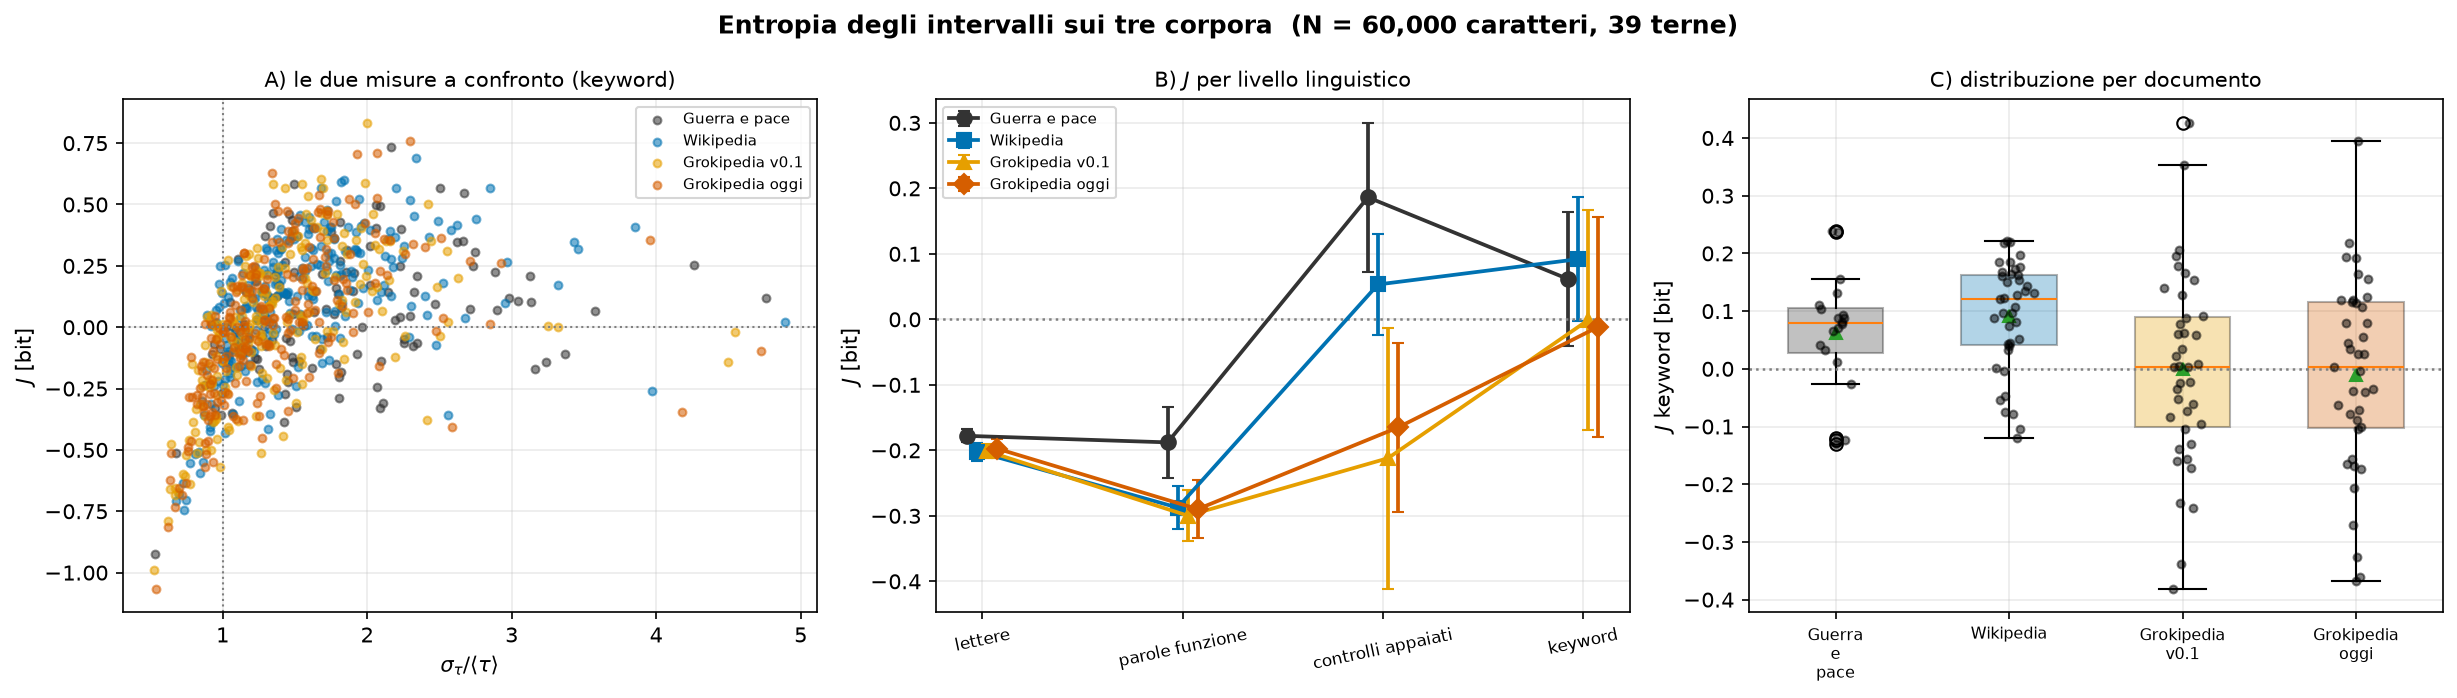
\includegraphics[width=\textwidth]{figure/cap5_entropia_intervalli.png}
  \caption{Entropia degli intervalli. A: relazione fra $J$ e coefficiente di
  variazione sulle parole chiave, un punto per sequenza. B: $J$ ai quattro
  livelli linguistici, con deviazioni standard fra testi; valori negativi
  indicano intervalli più regolari di un processo di Poisson. C: distribuzione
  di $J$ sulle parole chiave documento per documento. La misura è invariante per
  dilatazione dell'asse dei caratteri e non risente quindi della diversa
  lunghezza delle frasi nei due corpora enciclopedici.}
  \label{fig:entropia}
\end{figure}

% ---------------------------------------------------------------------
\section{Quanto pesa la definizione dei livelli lessicali}
\label{sec:effetto-stoplist}

Il paragrafo \emph{Come vengono separati i livelli lessicali} del
§\ref{sec:scelte} ha documentato l'estensione della lista chiusa di parole funzione da
\num{133} a \num{215} voci e la ragione per cui era necessaria. Questa sezione
riporta di quanto si spostano i risultati, perché lo spostamento non è
trascurabile e la scelta deve restare verificabile.

Il pannello A della Figura~\ref{fig:effetto-stoplist} riporta quali parole la
lista originaria lasciava passare fra le parole chiave di Grokipedia, e in
quante voci ciascuna: nell'elenco corrispondente di Wikipedia non ne compare
nessuna, e le sue sette parole sono distinte fra loro, ciascuna in una sola
voce.

\begin{table}[htbp]
  \centering
  \begin{tabular}{lcccc}
    \toprule
    & \multicolumn{2}{c}{lista originaria} & \multicolumn{2}{c}{lista estesa} \\
    \cmidrule(lr){2-3}\cmidrule(lr){4-5}
    & Wikipedia & Grok. oggi & Wikipedia & Grok. oggi \\
    \midrule
    keyword più bursty del controllo & $0.685$ & $0.630$ & $0.692$ & $0.740$ \\
    idem, su $\hat\gamma$ & $0.736$ & $0.663$ & $0.747$ & $0.791$ \\
    $\sigma_\tau/\langle\tau\rangle$ keyword & $1.530$ & $1.289$ & $1.536$ & $1.379$ \\
    divario appaiato, keyword & \multicolumn{2}{c}{$-0.230$} & \multicolumn{2}{c}{$-0.167$} \\
    divario appaiato, controlli & \multicolumn{2}{c}{$-0.122$} & \multicolumn{2}{c}{$-0.157$} \\
    $J$ keyword & $+0.086$ & $-0.069$ & $+0.092$ & $-0.011$ \\
    $\mu$ keyword & $2.38$ & $2.52$ & $2.37$ & $2.19$ \\
    quadrante basso-sinistra & $5.1\%$ & $24.5\%$ & $5.1\%$ & $14.3\%$ \\
    \bottomrule
  \end{tabular}
  \caption{Effetto della definizione dei livelli lessicali sui risultati del
  capitolo. Le righe dei divari appaiati riportano un solo valore perché
  misurano la differenza fra i due corpora. Le lettere e le parole funzione non
  compaiono perché nessuna parola cambia livello a quelle altezze: i loro valori
  coincidono a tutte le cifre riportate nel capitolo.}
  \label{tab:effetto-stoplist}
\end{table}

La Tabella~\ref{tab:effetto-stoplist} riporta il confronto. Tre risultati
cambiano in modo sostanziale. Il primo è il test interno: con la lista
originaria Grokipedia sembrava battere il proprio controllo appaiato meno spesso
di Wikipedia, e l'ordinamento fra i corpora appariva netto; con la lista estesa
l'ordine si inverte, e la differenza fra le due enciclopedie sparisce. Il
pannello B della figura mostra i due esiti sovrapposti. Il secondo è l'entropia
degli intervalli, il cui valore sulle parole chiave passa da $-0.069$ a
$-0.011$, cioè da un cambio di segno netto a uno indistinguibile da zero. Il
terzo è l'esponente di coda, che su Grokipedia scende da $2.52$ a $2.19$,
avvicinandosi a quello di Wikipedia anziché allontanarsene.

Restano invece stabili il divario appaiato complessivo, che si riduce da
$-0.230$ a $-0.167$ senza perdere significatività, il coefficiente di variazione
delle parole chiave, e l'intera decomposizione della~\eqref{eq:eq4}. Non si
muovono di una cifra, come è ovvio, i livelli delle lettere e delle parole
funzione.

La lezione metodologica vale al di là di questo caso. La distinzione fra
parole di contenuto e parole di servizio è la premessa dell'intero protocollo
di~\cite{altmann2012}, e viene qui operata da una lista chiusa che il paper
non specifica. Quando i corpora confrontati hanno abitudini lessicali diverse,
e un modello linguistico ne ha rispetto a un redattore umano, una lista
incompleta non introduce un rumore simmetrico: sposta sistematicamente in un
solo corpus il confine fra i due livelli, e produce un divario che non c'è.

\begin{figure}[htbp]
  \centering
  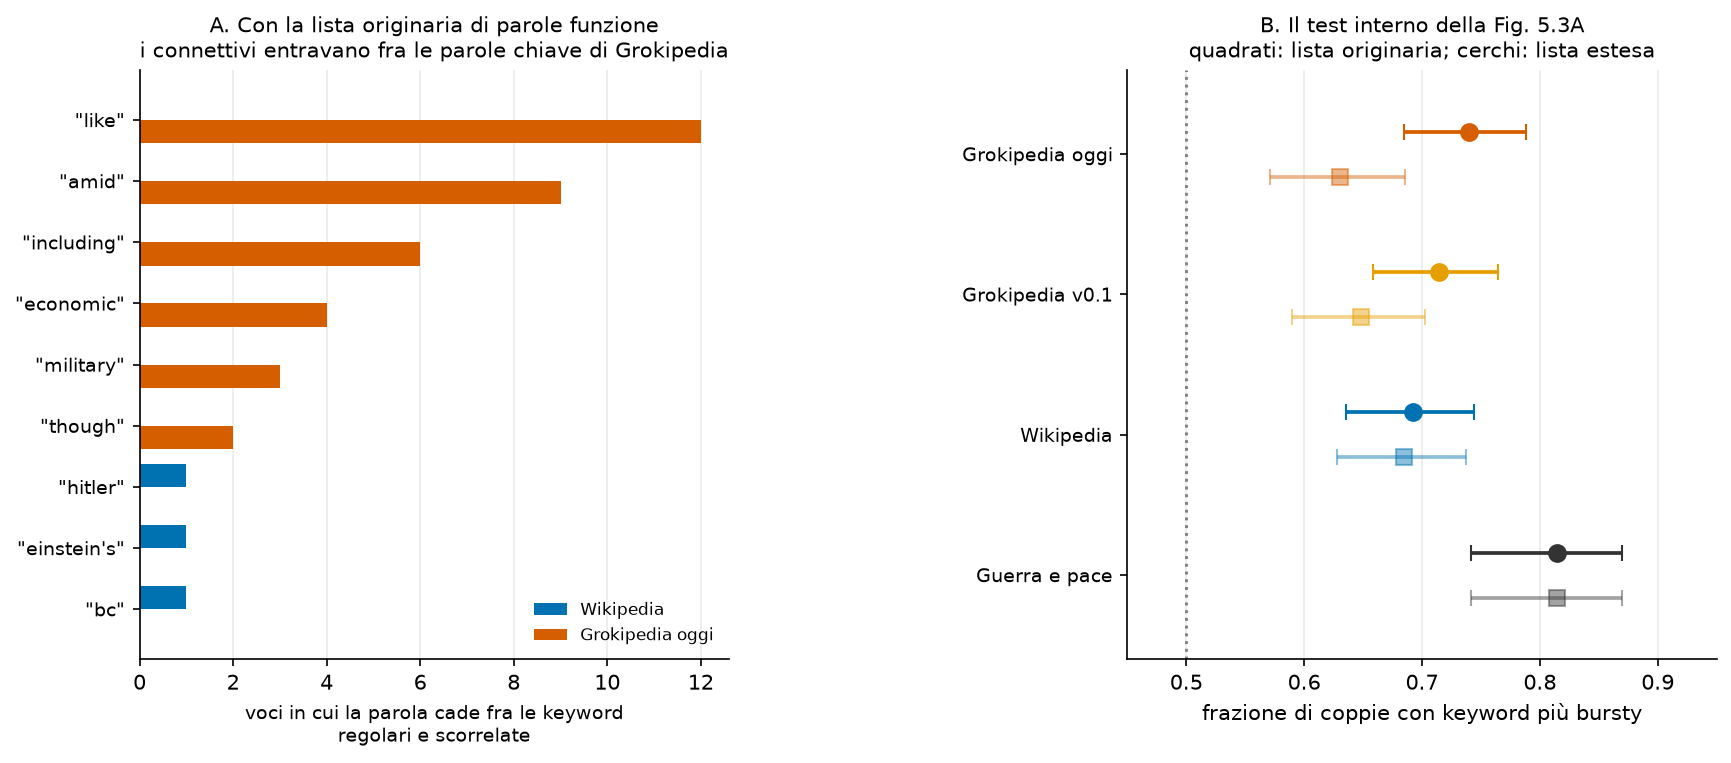
\includegraphics[width=\textwidth]{figure/cap5_effetto_stoplist.png}
  \caption{Effetto della definizione dei livelli lessicali. A: con la lista di
  funtori originaria, quali parole cadevano fra le parole chiave classificate
  come regolari e scorrelate, contate come numero di voci in cui ciò accadeva;
  le prime tre di Grokipedia sono connettivi, e in Wikipedia non compaiono. B:
  il test interno della Figura~\ref{fig:tre-corpora}A con le due
  classificazioni, quadrati per la lista originaria e cerchi per quella estesa,
  con intervalli di confidenza al $95\%$.}
  \label{fig:effetto-stoplist}
\end{figure}

% ---------------------------------------------------------------------
\section{Che cosa il testo generato non riproduce}
\label{sec:sintesi-cap5}

Il testo generato possiede correlazioni a lungo raggio, e ai livelli bassi della
gerarchia linguistica le possiede quasi nella stessa misura del testo umano:
sulle lettere i quattro corpora sono indistinguibili per coefficiente di
variazione, per entropia degli intervalli e per quota di burstiness, e sulle
parole funzione la differenza è piccola, benché significativa. Al livello delle parole il divario si apre, e vale più di un ordine
di grandezza rispetto a quello misurato sui caratteri.

Il divario non distingue però le parole che portano il contenuto dai controlli a
frequenza appaiata. I due valori sono quasi uguali alla lunghezza di lavoro,
$-0.157$ e $-0.167$, e si invertono a quella di controllo
(§\ref{sec:robustezza-neff}); e il test che chiede se la parola chiave superi il
proprio controllo \emph{dentro lo stesso testo} dà a Grokipedia un esito pari a
quello di Wikipedia, anzi lievemente migliore. Il meccanismo descritto
in~\cite{altmann2012} è dunque presente nel testo generato, e con la stessa
efficacia: ciò che manca è l'ampiezza con cui le parole, di contenuto e non, si
addensano.

Non si tratta dunque di una persistenza tematica assente, perché la distinzione
fra parole tematiche e parole ordinarie il modello la produce; si tratta di una
compressione uniforme della variabilità lessicale, che riduce la burstiness di
tutte le parole senza alterare il rapporto fra le une e le altre. Vale ancora la
distinzione posta nel §\ref{sec:intro-linguaggio} fra riprodurre le proprietà
statistiche del linguaggio e riprodurre il meccanismo che le genera, ma
applicata a un livello più basso di quanto la prima lettura suggerisse.

Ciò che il capitolo misura è la distanza fra due enciclopedie appaiate titolo
per titolo, e null'altro. Il deficit è osservato su Grokipedia, cioè su un unico
sistema generativo, in un unico dominio e in una sola lingua: nulla di quanto
riportato qui stabilisce che sia una proprietà dei modelli linguistici in
generale anziché di quel sistema. Il Capitolo~\ref{cap:risultati1} non offre un
appoggio indipendente su questo punto: misura un altro corpus, con grandezze
che non arrivano al livello a cui il divario si manifesta.


% =====================================================================
%  Capitolo 6 — Discussione e conclusioni
%  Incluso da main.tex con % =====================================================================
%  Capitolo 6 — Discussione e conclusioni
%  Incluso da main.tex con % =====================================================================
%  Capitolo 6 — Discussione e conclusioni
%  Incluso da main.tex con \input{capitolo6_discussione_conclusioni}
%
%  Non introduce misure nuove: tutti i numeri citati provengono dai
%  Capitoli 3, 4 e 5 e sono riportati con il riferimento alla sezione
%  in cui sono stati ottenuti.
% =====================================================================

\chapter{Discussione e conclusioni}
\label{cap:discussione}

I due capitoli sperimentali rispondono ciascuno a metà della domanda posta nel
§\ref{sec:intro-domanda}, e lo fanno su corpora diversi. Il
Capitolo~\ref{cap:risultati1} stabilisce dove un modello produca linguaggio; il
Capitolo~\ref{cap:risultati2} stabilisce che cosa manchi al testo generato là
dove esso è ben formato. Sono due risultati indipendenti, uno positivo e uno negativo, e restano tali:
i corpora sono diversi e le condizioni di generazione del secondo non sono
note, per cui nessuna delle due misure può essere usata come conferma
dell'altra.

Il capitolo non rimisura nulla: il §\ref{sec:risposta} enuncia i due risultati
e il §\ref{sec:conclusioni} raccoglie le conclusioni.


% ---------------------------------------------------------------------
\section{I due risultati}
\label{sec:risposta}
\label{sec:convergenza-cosa}
\label{sec:persistenza}

La domanda del §\ref{sec:intro-domanda} è: quali proprietà statistiche del
linguaggio un modello riproduce effettivamente, e a quale livello della
gerarchia linguistica smette di riprodurle? I due capitoli sperimentali ne
danno due metà, misurate su corpora diversi e con protocolli diversi.

\paragraph{Esito dello sweep di temperatura.}
Un modello riproduce bene le regolarità che dipendono dalla distribuzione delle
frequenze e dalla struttura locale della successione: la legge di Zipf, la
crescita del vocabolario, la comprimibilità, le correlazioni misurate sui
caratteri. Lo fa però soltanto dentro una finestra stretta. Otto criteri tratti
da quattro lavori indipendenti, costruiti per scopi diversi e mai progettati per
concordare, danno una mediana identica $T = 1.0$ per tutti e cinque i modelli,
senza dipendenza rilevabile dalla dimensione (§\ref{sec:tstar}); la transizione
si consuma quasi interamente fra $T = 0.9$ e $T = 1.0$, dove l'entropia passa da
$0.332$ a $5.77$ bit per carattere e il parametro di periodicità cade di un
fattore cinquanta. Fuori da quella finestra il testo degenera nei due modi
opposti descritti nel §\ref{sec:fallimenti}, e i documenti che sostengono
un'analisi semantica sono due su \num{242}. Il capitolo lascia però aperta la
domanda che lo ha originato, perché gli otto criteri che convergono sono tutti
definiti sui conteggi o sul livello dei caratteri: la temperatura che
individuano è quella a cui il testo generato somiglia di più a quello umano
secondo i livelli su cui la somiglianza è più facile, e nulla in quel capitolo
dice che in quel punto il testo sia organizzato attorno a un contenuto.

\paragraph{Esito della misura di burstiness.}
Il secondo capitolo sperimentale porta la domanda al livello che il primo non
raggiunge, su un corpus in cui la qualità del testo non è una variabile. In
prosa enciclopedica ben formata il testo generato conserva l'apparenza
statistica di quello umano: le parole chiave restano più \emph{bursty} dei
propri controlli a frequenza appaiata anche in Grokipedia, e vi riescono quanto
in Wikipedia, $0.740$ contro $0.692$ (§\ref{sec:tre-corpora}). Cambia
l'intensità. Sulle lettere i quattro corpora sono indistinguibili; il divario si
apre al livello delle parole, dove vale più di un ordine di grandezza rispetto a
quello misurato sui caratteri, e l'entropia degli intervalli lo conferma
eliminando l'effetto della diversa lunghezza delle frasi, con una differenza
appaiata di $-0.105$ bit e significatività inferiore a $10^{-3}$
(§\ref{sec:entropia-intervalli}). Dentro il livello lessicale, però, il divario
non separa le parole di contenuto dai controlli a frequenza appaiata. Il
risultato riguarda un solo sistema generativo, un solo dominio e una sola
lingua, e vale per il testo generato \emph{ben formato}: le condizioni di
campionamento con cui Grokipedia è stata prodotta non sono note, e non è
possibile collocarla sull'asse di temperatura del primo capitolo.


% ---------------------------------------------------------------------
\section{Conclusioni}
\label{sec:conclusioni}

Il lavoro ha misurato le proprietà statistiche del linguaggio generato lungo
due assi, la temperatura di campionamento e la gerarchia dei livelli
linguistici.

\begin{enumerate}
  \item \textbf{Esiste una temperatura privilegiata, e la sua posizione è
    comune.} Otto criteri tratti da quattro lavori indipendenti, mai progettati
    per concordare, danno mediana $T = 1.0$ su tutti e cinque i modelli, senza
    dipendenza rilevabile dalla dimensione. È il risultato empirico più solido
    della tesi.

  \item \textbf{La finestra è stretta e la qualità dell'ottimo non è
    garantita.} La transizione si consuma fra $T = 0.9$ e $T = 1.0$, dove
    l'entropia passa da $0.332$ a $5.77$ bit per carattere. Due modelli su
    cinque portano il MAPE al livello umano e gli altri no: l'esistenza
    dell'ottimo è un fatto generale, la sua profondità una proprietà del
    singolo modello.

  \item \textbf{Il testo generato riproduce le regolarità dei livelli bassi
    della gerarchia e perde terreno salendo.} Sulle lettere i quattro corpora
    sono indistinguibili per tutte e tre le misure impiegate; il divario si apre
    al livello delle parole e vi supera di un ordine di grandezza quello
    misurato sui caratteri. Dentro quel livello, però, non separa le parole di
    contenuto dai controlli a frequenza appaiata.

  \item \textbf{Il deficit è di intensità, non di natura.} Il meccanismo
    descritto in~\cite{altmann2012} è presente anche nella prosa generata e vi
    si decompone nelle stesse proporzioni; le sue parole chiave battono i
    propri controlli a frequenza appaiata quanto quelle di Wikipedia. Manca il
    quanto, non il come.

  \item \textbf{La convergenza dei criteri riguarda i livelli bassi.} Gli otto
    criteri che individuano $T = 1.0$ sono tutti definiti sui conteggi o sui
    caratteri. Se il linguaggio naturale giace sulla superficie critica, come
    sostenuto in~\cite{nakaishi2024}, questo lavoro mostra che vi si arriva
    facendo coincidere le statistiche di quei livelli; che cosa accada ai
    livelli alti in quel punto resta fuori da ciò che lo sweep può misurare,
    perché in quel punto i documenti non degenerati sono due su \num{242}.
\end{enumerate}

I contributi di metodo sono elencati nel §\ref{sec:intro-domanda}. I due
principali sono la stima diretta
dell'esponente di coda e del cut-off, che in~\cite{altmann2012} sono adottati
senza misura e che qui risultano corretti nel valore ma inutilizzabili per
ordinare i corpora, e l'entropia degli intervalli $J$
(§\ref{sec:entropia-intervalli-def}), che non risente della diversa lunghezza
delle frasi ed è circa tre volte più stabile rispetto alla lunghezza di analisi
della misura che sostituisce.

Si torni alla Tabella~\ref{tab:tre-regimi}, da cui il lavoro è partito. Delle
quattro sequenze che vi compaiono una sola è linguaggio, e un unico modello
percorre le altre tre cambiando un solo parametro, sfiorando la seconda in due
documenti su \num{242}. Il testo generato sta fra l'ordine e il disordine, ma
non nel modo in cui vi sta il linguaggio: possiede le regolarità che si
misurano sui conteggi e sui caratteri, e possiede in misura ridotta quella che
nasce dall'essere un discorso su qualcosa. Riprodurre le proprietà statistiche
del linguaggio non equivale a riprodurre il meccanismo che le genera, ed è la
distinzione con cui il §\ref{sec:intro-linguaggio} era partito.

%
%  Non introduce misure nuove: tutti i numeri citati provengono dai
%  Capitoli 3, 4 e 5 e sono riportati con il riferimento alla sezione
%  in cui sono stati ottenuti.
% =====================================================================

\chapter{Discussione e conclusioni}
\label{cap:discussione}

I due capitoli sperimentali rispondono ciascuno a metà della domanda posta nel
§\ref{sec:intro-domanda}, e lo fanno su corpora diversi. Il
Capitolo~\ref{cap:risultati1} stabilisce dove un modello produca linguaggio; il
Capitolo~\ref{cap:risultati2} stabilisce che cosa manchi al testo generato là
dove esso è ben formato. Sono due risultati indipendenti, uno positivo e uno negativo, e restano tali:
i corpora sono diversi e le condizioni di generazione del secondo non sono
note, per cui nessuna delle due misure può essere usata come conferma
dell'altra.

Il capitolo non rimisura nulla: il §\ref{sec:risposta} enuncia i due risultati
e il §\ref{sec:conclusioni} raccoglie le conclusioni.


% ---------------------------------------------------------------------
\section{I due risultati}
\label{sec:risposta}
\label{sec:convergenza-cosa}
\label{sec:persistenza}

La domanda del §\ref{sec:intro-domanda} è: quali proprietà statistiche del
linguaggio un modello riproduce effettivamente, e a quale livello della
gerarchia linguistica smette di riprodurle? I due capitoli sperimentali ne
danno due metà, misurate su corpora diversi e con protocolli diversi.

\paragraph{Esito dello sweep di temperatura.}
Un modello riproduce bene le regolarità che dipendono dalla distribuzione delle
frequenze e dalla struttura locale della successione: la legge di Zipf, la
crescita del vocabolario, la comprimibilità, le correlazioni misurate sui
caratteri. Lo fa però soltanto dentro una finestra stretta. Otto criteri tratti
da quattro lavori indipendenti, costruiti per scopi diversi e mai progettati per
concordare, danno una mediana identica $T = 1.0$ per tutti e cinque i modelli,
senza dipendenza rilevabile dalla dimensione (§\ref{sec:tstar}); la transizione
si consuma quasi interamente fra $T = 0.9$ e $T = 1.0$, dove l'entropia passa da
$0.332$ a $5.77$ bit per carattere e il parametro di periodicità cade di un
fattore cinquanta. Fuori da quella finestra il testo degenera nei due modi
opposti descritti nel §\ref{sec:fallimenti}, e i documenti che sostengono
un'analisi semantica sono due su \num{242}. Il capitolo lascia però aperta la
domanda che lo ha originato, perché gli otto criteri che convergono sono tutti
definiti sui conteggi o sul livello dei caratteri: la temperatura che
individuano è quella a cui il testo generato somiglia di più a quello umano
secondo i livelli su cui la somiglianza è più facile, e nulla in quel capitolo
dice che in quel punto il testo sia organizzato attorno a un contenuto.

\paragraph{Esito della misura di burstiness.}
Il secondo capitolo sperimentale porta la domanda al livello che il primo non
raggiunge, su un corpus in cui la qualità del testo non è una variabile. In
prosa enciclopedica ben formata il testo generato conserva l'apparenza
statistica di quello umano: le parole chiave restano più \emph{bursty} dei
propri controlli a frequenza appaiata anche in Grokipedia, e vi riescono quanto
in Wikipedia, $0.740$ contro $0.692$ (§\ref{sec:tre-corpora}). Cambia
l'intensità. Sulle lettere i quattro corpora sono indistinguibili; il divario si
apre al livello delle parole, dove vale più di un ordine di grandezza rispetto a
quello misurato sui caratteri, e l'entropia degli intervalli lo conferma
eliminando l'effetto della diversa lunghezza delle frasi, con una differenza
appaiata di $-0.105$ bit e significatività inferiore a $10^{-3}$
(§\ref{sec:entropia-intervalli}). Dentro il livello lessicale, però, il divario
non separa le parole di contenuto dai controlli a frequenza appaiata. Il
risultato riguarda un solo sistema generativo, un solo dominio e una sola
lingua, e vale per il testo generato \emph{ben formato}: le condizioni di
campionamento con cui Grokipedia è stata prodotta non sono note, e non è
possibile collocarla sull'asse di temperatura del primo capitolo.


% ---------------------------------------------------------------------
\section{Conclusioni}
\label{sec:conclusioni}

Il lavoro ha misurato le proprietà statistiche del linguaggio generato lungo
due assi, la temperatura di campionamento e la gerarchia dei livelli
linguistici.

\begin{enumerate}
  \item \textbf{Esiste una temperatura privilegiata, e la sua posizione è
    comune.} Otto criteri tratti da quattro lavori indipendenti, mai progettati
    per concordare, danno mediana $T = 1.0$ su tutti e cinque i modelli, senza
    dipendenza rilevabile dalla dimensione. È il risultato empirico più solido
    della tesi.

  \item \textbf{La finestra è stretta e la qualità dell'ottimo non è
    garantita.} La transizione si consuma fra $T = 0.9$ e $T = 1.0$, dove
    l'entropia passa da $0.332$ a $5.77$ bit per carattere. Due modelli su
    cinque portano il MAPE al livello umano e gli altri no: l'esistenza
    dell'ottimo è un fatto generale, la sua profondità una proprietà del
    singolo modello.

  \item \textbf{Il testo generato riproduce le regolarità dei livelli bassi
    della gerarchia e perde terreno salendo.} Sulle lettere i quattro corpora
    sono indistinguibili per tutte e tre le misure impiegate; il divario si apre
    al livello delle parole e vi supera di un ordine di grandezza quello
    misurato sui caratteri. Dentro quel livello, però, non separa le parole di
    contenuto dai controlli a frequenza appaiata.

  \item \textbf{Il deficit è di intensità, non di natura.} Il meccanismo
    descritto in~\cite{altmann2012} è presente anche nella prosa generata e vi
    si decompone nelle stesse proporzioni; le sue parole chiave battono i
    propri controlli a frequenza appaiata quanto quelle di Wikipedia. Manca il
    quanto, non il come.

  \item \textbf{La convergenza dei criteri riguarda i livelli bassi.} Gli otto
    criteri che individuano $T = 1.0$ sono tutti definiti sui conteggi o sui
    caratteri. Se il linguaggio naturale giace sulla superficie critica, come
    sostenuto in~\cite{nakaishi2024}, questo lavoro mostra che vi si arriva
    facendo coincidere le statistiche di quei livelli; che cosa accada ai
    livelli alti in quel punto resta fuori da ciò che lo sweep può misurare,
    perché in quel punto i documenti non degenerati sono due su \num{242}.
\end{enumerate}

I contributi di metodo sono elencati nel §\ref{sec:intro-domanda}. I due
principali sono la stima diretta
dell'esponente di coda e del cut-off, che in~\cite{altmann2012} sono adottati
senza misura e che qui risultano corretti nel valore ma inutilizzabili per
ordinare i corpora, e l'entropia degli intervalli $J$
(§\ref{sec:entropia-intervalli-def}), che non risente della diversa lunghezza
delle frasi ed è circa tre volte più stabile rispetto alla lunghezza di analisi
della misura che sostituisce.

Si torni alla Tabella~\ref{tab:tre-regimi}, da cui il lavoro è partito. Delle
quattro sequenze che vi compaiono una sola è linguaggio, e un unico modello
percorre le altre tre cambiando un solo parametro, sfiorando la seconda in due
documenti su \num{242}. Il testo generato sta fra l'ordine e il disordine, ma
non nel modo in cui vi sta il linguaggio: possiede le regolarità che si
misurano sui conteggi e sui caratteri, e possiede in misura ridotta quella che
nasce dall'essere un discorso su qualcosa. Riprodurre le proprietà statistiche
del linguaggio non equivale a riprodurre il meccanismo che le genera, ed è la
distinzione con cui il §\ref{sec:intro-linguaggio} era partito.

%
%  Non introduce misure nuove: tutti i numeri citati provengono dai
%  Capitoli 3, 4 e 5 e sono riportati con il riferimento alla sezione
%  in cui sono stati ottenuti.
% =====================================================================

\chapter{Discussione e conclusioni}
\label{cap:discussione}

I due capitoli sperimentali rispondono ciascuno a metà della domanda posta nel
§\ref{sec:intro-domanda}, e lo fanno su corpora diversi. Il
Capitolo~\ref{cap:risultati1} stabilisce dove un modello produca linguaggio; il
Capitolo~\ref{cap:risultati2} stabilisce che cosa manchi al testo generato là
dove esso è ben formato. Sono due risultati indipendenti, uno positivo e uno negativo, e restano tali:
i corpora sono diversi e le condizioni di generazione del secondo non sono
note, per cui nessuna delle due misure può essere usata come conferma
dell'altra.

Il capitolo non rimisura nulla: il §\ref{sec:risposta} enuncia i due risultati
e il §\ref{sec:conclusioni} raccoglie le conclusioni.


% ---------------------------------------------------------------------
\section{I due risultati}
\label{sec:risposta}
\label{sec:convergenza-cosa}
\label{sec:persistenza}

La domanda del §\ref{sec:intro-domanda} è: quali proprietà statistiche del
linguaggio un modello riproduce effettivamente, e a quale livello della
gerarchia linguistica smette di riprodurle? I due capitoli sperimentali ne
danno due metà, misurate su corpora diversi e con protocolli diversi.

\paragraph{Esito dello sweep di temperatura.}
Un modello riproduce bene le regolarità che dipendono dalla distribuzione delle
frequenze e dalla struttura locale della successione: la legge di Zipf, la
crescita del vocabolario, la comprimibilità, le correlazioni misurate sui
caratteri. Lo fa però soltanto dentro una finestra stretta. Otto criteri tratti
da quattro lavori indipendenti, costruiti per scopi diversi e mai progettati per
concordare, danno una mediana identica $T = 1.0$ per tutti e cinque i modelli,
senza dipendenza rilevabile dalla dimensione (§\ref{sec:tstar}); la transizione
si consuma quasi interamente fra $T = 0.9$ e $T = 1.0$, dove l'entropia passa da
$0.332$ a $5.77$ bit per carattere e il parametro di periodicità cade di un
fattore cinquanta. Fuori da quella finestra il testo degenera nei due modi
opposti descritti nel §\ref{sec:fallimenti}, e i documenti che sostengono
un'analisi semantica sono due su \num{242}. Il capitolo lascia però aperta la
domanda che lo ha originato, perché gli otto criteri che convergono sono tutti
definiti sui conteggi o sul livello dei caratteri: la temperatura che
individuano è quella a cui il testo generato somiglia di più a quello umano
secondo i livelli su cui la somiglianza è più facile, e nulla in quel capitolo
dice che in quel punto il testo sia organizzato attorno a un contenuto.

\paragraph{Esito della misura di burstiness.}
Il secondo capitolo sperimentale porta la domanda al livello che il primo non
raggiunge, su un corpus in cui la qualità del testo non è una variabile. In
prosa enciclopedica ben formata il testo generato conserva l'apparenza
statistica di quello umano: le parole chiave restano più \emph{bursty} dei
propri controlli a frequenza appaiata anche in Grokipedia, e vi riescono quanto
in Wikipedia, $0.740$ contro $0.692$ (§\ref{sec:tre-corpora}). Cambia
l'intensità. Sulle lettere i quattro corpora sono indistinguibili; il divario si
apre al livello delle parole, dove vale più di un ordine di grandezza rispetto a
quello misurato sui caratteri, e l'entropia degli intervalli lo conferma
eliminando l'effetto della diversa lunghezza delle frasi, con una differenza
appaiata di $-0.105$ bit e significatività inferiore a $10^{-3}$
(§\ref{sec:entropia-intervalli}). Dentro il livello lessicale, però, il divario
non separa le parole di contenuto dai controlli a frequenza appaiata. Il
risultato riguarda un solo sistema generativo, un solo dominio e una sola
lingua, e vale per il testo generato \emph{ben formato}: le condizioni di
campionamento con cui Grokipedia è stata prodotta non sono note, e non è
possibile collocarla sull'asse di temperatura del primo capitolo.


% ---------------------------------------------------------------------
\section{Conclusioni}
\label{sec:conclusioni}

Il lavoro ha misurato le proprietà statistiche del linguaggio generato lungo
due assi, la temperatura di campionamento e la gerarchia dei livelli
linguistici.

\begin{enumerate}
  \item \textbf{Esiste una temperatura privilegiata, e la sua posizione è
    comune.} Otto criteri tratti da quattro lavori indipendenti, mai progettati
    per concordare, danno mediana $T = 1.0$ su tutti e cinque i modelli, senza
    dipendenza rilevabile dalla dimensione. È il risultato empirico più solido
    della tesi.

  \item \textbf{La finestra è stretta e la qualità dell'ottimo non è
    garantita.} La transizione si consuma fra $T = 0.9$ e $T = 1.0$, dove
    l'entropia passa da $0.332$ a $5.77$ bit per carattere. Due modelli su
    cinque portano il MAPE al livello umano e gli altri no: l'esistenza
    dell'ottimo è un fatto generale, la sua profondità una proprietà del
    singolo modello.

  \item \textbf{Il testo generato riproduce le regolarità dei livelli bassi
    della gerarchia e perde terreno salendo.} Sulle lettere i quattro corpora
    sono indistinguibili per tutte e tre le misure impiegate; il divario si apre
    al livello delle parole e vi supera di un ordine di grandezza quello
    misurato sui caratteri. Dentro quel livello, però, non separa le parole di
    contenuto dai controlli a frequenza appaiata.

  \item \textbf{Il deficit è di intensità, non di natura.} Il meccanismo
    descritto in~\cite{altmann2012} è presente anche nella prosa generata e vi
    si decompone nelle stesse proporzioni; le sue parole chiave battono i
    propri controlli a frequenza appaiata quanto quelle di Wikipedia. Manca il
    quanto, non il come.

  \item \textbf{La convergenza dei criteri riguarda i livelli bassi.} Gli otto
    criteri che individuano $T = 1.0$ sono tutti definiti sui conteggi o sui
    caratteri. Se il linguaggio naturale giace sulla superficie critica, come
    sostenuto in~\cite{nakaishi2024}, questo lavoro mostra che vi si arriva
    facendo coincidere le statistiche di quei livelli; che cosa accada ai
    livelli alti in quel punto resta fuori da ciò che lo sweep può misurare,
    perché in quel punto i documenti non degenerati sono due su \num{242}.
\end{enumerate}

I contributi di metodo sono elencati nel §\ref{sec:intro-domanda}. I due
principali sono la stima diretta
dell'esponente di coda e del cut-off, che in~\cite{altmann2012} sono adottati
senza misura e che qui risultano corretti nel valore ma inutilizzabili per
ordinare i corpora, e l'entropia degli intervalli $J$
(§\ref{sec:entropia-intervalli-def}), che non risente della diversa lunghezza
delle frasi ed è circa tre volte più stabile rispetto alla lunghezza di analisi
della misura che sostituisce.

Si torni alla Tabella~\ref{tab:tre-regimi}, da cui il lavoro è partito. Delle
quattro sequenze che vi compaiono una sola è linguaggio, e un unico modello
percorre le altre tre cambiando un solo parametro, sfiorando la seconda in due
documenti su \num{242}. Il testo generato sta fra l'ordine e il disordine, ma
non nel modo in cui vi sta il linguaggio: possiede le regolarità che si
misurano sui conteggi e sui caratteri, e possiede in misura ridotta quella che
nasce dall'essere un discorso su qualcosa. Riprodurre le proprietà statistiche
del linguaggio non equivale a riprodurre il meccanismo che le genera, ed è la
distinzione con cui il §\ref{sec:intro-linguaggio} era partito.


% =====================================================================
%  APPENDICI
% =====================================================================
\appendix

% =====================================================================
%  Appendice B — Codice e dati
%  Inclusa da main.tex dopo \appendix
% =====================================================================

\chapter{Codice e dati}
\label{app:codice}

Il codice di analisi e di generazione, i risultati intermedi, le figure e i
dataset di testo generato sono raccolti in un repository pubblico:

\begin{center}
\footnotesize
\url{https://github.com/SamueleZurlo/Fra-ordine-e-disordine-Proprieta-statistiche-del-linguaggio-generato-da-Large-Language-Model}
\end{center}

\noindent
Il repository contiene i notebook che producono ogni figura e ogni tabella di
questa tesi, i file di risultato in formato aperto e i \num{242} documenti
generati lungo lo sweep di temperatura, con il registro delle condizioni di
produzione di ciascuno: temperatura, seme, parametri di campionamento, numero
di riprese e posizioni dei token di fine sequenza. Il codice è distribuito con
licenza MIT, i dati e le figure con licenza Creative Commons Attribuzione 4.0.

Non vi sono inclusi i corpora di provenienza esterna, che sono materiale
altrui. Al loro posto il file \texttt{FONTI.md} riporta, per ciascun corpus,
la fonte, la data di acquisizione, gli identificatori necessari a riscaricarlo
e un'impronta crittografica dei file impiegati, con la quale chi ripeta
l'acquisizione può stabilire se dispone degli stessi byte. Le voci di
Wikipedia sono riscaricabili a partire dall'elenco dei titoli, anch'esso
incluso; le catture di Grokipedia v0.1 sono permanenti sull'Internet Archive;
il romanzo di riferimento è pubblico dominio.

Fa eccezione la versione attuale di Grokipedia. Come discusso nel
§\ref{sec:paternita}, la piattaforma non pubblica una cronologia delle
revisioni e riscrive le voci senza conservarne lo stato precedente: le catture
impiegate qui sono l'unico testimone di quel testo, e le misure del
Capitolo~\ref{cap:risultati2} che vi si appoggiano possono essere ricontrollate
nei valori derivati ma non rifatte a partire dalla fonte. È un limite della
fonte, non del protocollo, ed è la ragione per cui il §\ref{sec:corpora}
conserva copia locale di tutti i corpora scaricati.


% =====================================================================
%  BIBLIOGRAFIA
% =====================================================================
\begin{thebibliography}{99}

% ---- leggi di scala del vocabolario ---------------------------------
\bibitem{zipf1949}
G.~K. Zipf,
\emph{Human Behavior and the Principle of Least Effort},
Addison-Wesley (1949).

\bibitem{herdan1964}
G.~Herdan,
\emph{Quantitative Linguistics},
Butterworths (1964).

\bibitem{heaps1978}
H.~S. Heaps,
\emph{Information Retrieval: Computational and Theoretical Aspects},
Academic Press (1978).

\bibitem{mandelbrot1953}
B.~Mandelbrot,
\emph{An informational theory of the statistical structure of language},
in W.~Jackson (a cura di), \emph{Communication Theory}, Butterworths,
486--502 (1953).

\bibitem{piantadosi2014}
S.~T. Piantadosi,
\emph{Zipf's word frequency law in natural language: a critical review and
future directions},
Psychonomic Bulletin \& Review \textbf{21}, 1112--1130 (2014).

% ---- correlazioni a lungo raggio ------------------------------------
\bibitem{altmann2012}
E.~G. Altmann, G.~Cristadoro, M.~Degli Esposti,
\emph{On the origin of long-range correlations in texts},
Proc. Natl. Acad. Sci. USA \textbf{109}(29), 11582--11587 (2012).

\bibitem{montemurro2002}
M.~A. Montemurro, P.~A. Pury,
\emph{Long-range fractal correlations in literary corpora},
Fractals \textbf{10}(4), 451--461 (2002).

\bibitem{peng1994}
C.-K. Peng, S.~V. Buldyrev, S.~Havlin, M.~Simons, H.~E. Stanley,
A.~L. Goldberger,
\emph{Mosaic organization of DNA nucleotides},
Phys. Rev. E \textbf{49}(2), 1685--1689 (1994).

\bibitem{kantelhardt2001}
J.~W. Kantelhardt, E.~Koscielny-Bunde, H.~H.~A. Rego, S.~Havlin, A.~Bunde,
\emph{Detecting long-range correlations with detrended fluctuation analysis},
Physica A \textbf{295}(3--4), 441--454 (2001).

\bibitem{goh2008}
K.-I. Goh, A.-L. Barabási,
\emph{Burstiness and memory in complex systems},
EPL \textbf{81}(4), 48002 (2008).

% ---- entropia e compressione ----------------------------------------
\bibitem{vasicek1976}
O.~Vasicek.
\newblock A test for normality based on sample entropy.
\newblock \emph{Journal of the Royal Statistical Society B}, 38(1):54--59, 1976.

\bibitem{shannon1948}
C.~E. Shannon,
\emph{A mathematical theory of communication},
Bell System Technical Journal \textbf{27}(3), 379--423 (1948).

\bibitem{cover2006}
T.~M. Cover, J.~A. Thomas,
\emph{Elements of Information Theory}, 2ª ed.,
Wiley-Interscience (2006).

\bibitem{ziv1977}
J.~Ziv, A.~Lempel,
\emph{A universal algorithm for sequential data compression},
IEEE Trans. Inf. Theory \textbf{23}(3), 337--343 (1977).

\bibitem{ziv1993}
J.~Ziv, N.~Merhav,
\emph{A measure of relative entropy between individual sequences with
application to universal classification},
IEEE Trans. Inf. Theory \textbf{39}(4), 1270--1279 (1993).

\bibitem{li2004}
M.~Li, X.~Chen, X.~Li, B.~Ma, P.~M.~B. Vitányi,
\emph{The similarity metric},
IEEE Trans. Inf. Theory \textbf{50}(12), 3250--3264 (2004).

\bibitem{hadad2026}
O.~Hadad, E.~Loru, J.~Nudo, N.~Di Marco, M.~Cinelli, W.~Quattrociocchi,
\emph{The statistical signature of LLMs},
arXiv:2602.18152 (2026).

% ---- generazione automatica del testo --------------------------------
\bibitem{ackley1985}
D.~H. Ackley, G.~E. Hinton, T.~J. Sejnowski,
\emph{A learning algorithm for Boltzmann machines},
Cognitive Science \textbf{9}(1), 147--169 (1985).

\bibitem{vaswani2017}
A.~Vaswani, N.~Shazeer, N.~Parmar, J.~Uszkoreit, L.~Jones, A.~N. Gomez,
Ł.~Kaiser, I.~Polosukhin,
\emph{Attention is all you need},
Advances in Neural Information Processing Systems \textbf{30} (2017).

\bibitem{fan2018}
A.~Fan, M.~Lewis, Y.~Dauphin,
\emph{Hierarchical neural story generation},
Proc. of ACL 2018, 889--898.

\bibitem{holtzman2020}
A.~Holtzman, J.~Buys, L.~Du, M.~Forbes, Y.~Choi,
\emph{The curious case of neural text degeneration},
International Conference on Learning Representations (2020).

\bibitem{lippi2019}
M.~Lippi, M.~A. Montemurro, M.~Degli Esposti, G.~Cristadoro,
\emph{Natural language statistical features of LSTM-generated texts},
IEEE Trans. Neural Netw. Learn. Syst. \textbf{30}(11), 3326--3337 (2019).

% ---- fasi e stato critico -------------------------------------------
\bibitem{ehrenfest1933}
P.~Ehrenfest,
\emph{Phasenumwandlungen im ueblichen und erweiterten Sinn, classifiziert nach
den entsprechenden Singularitaeten des thermodynamischen Potentiales},
Proc. Royal Acad. Amsterdam \textbf{36}, 153--157 (1933).

\bibitem{nakaishi2024}
K.~Nakaishi, Y.~Nishikawa, K.~Hukushima,
\emph{Phase transition in large language models and the criticality of natural
languages},
arXiv:2406.05335v3 (2026).

\bibitem{mikhaylovskiy2023}
N.~Mikhaylovskiy,
\emph{Long story generation challenge},
Proc. of the 16th International Natural Language Generation Conference:
Generation Challenges, 10--16 (2023).

\bibitem{mikhaylovskiy2025states}
N.~Mikhaylovskiy,
\emph{States of LLM-generated texts and phase transitions between them},
First Conference of Mathematics of AI (MathAI 2025), arXiv:2503.06330.

\bibitem{mikhaylovskiy2025zipf}
N.~Mikhaylovskiy,
\emph{Zipf's and Heaps' laws for tokens and LLM-generated texts},
Findings of the Association for Computational Linguistics: EMNLP 2025,
15469--15481.

\end{thebibliography}

% =====================================================================
%  RINGRAZIAMENTI
% =====================================================================
% =====================================================================
%  Ringraziamenti
%  Incluso da main.tex dopo la bibliografia.
%  Il capitolo non e' numerato ma compare nell'indice.
% =====================================================================

\clearpage
\chapter*{Ringraziamenti}
\addcontentsline{toc}{chapter}{Ringraziamenti}

Ringrazio:

\begin{itemize}
  \setlength{\itemsep}{0.7em}

  \item i miei genitori, per gli sforzi e i sacrifici;

  \item le mie sorelle Noemi e Ginevra, soprattutto Ginevra;

  \item mia nonna Anna, per i panzerotti, e quel puzzolone del suo consorte,
    perché se non lo metto si offende;

  \item Elisabetta, che fa rima con polpetta;

  \item Chi è Mario?

  \item i miei cari compagni di classe Giulio e Davide, per le relazioni di
    laboratorio e gli appunti rubati;

  \item quella schifosa di Giulia, per avermi fatto conoscere Miro e Stefano
    (e \mbox{nient'altro});

  \item il professor Giannotte, per le lezioni di termodinamica, e il
    professor Termite, per le lezioni di C;

  \item il mio relatore, Mirko Degli Esposti, per tutte le risate durante il
    corso di meccanica analitica.
\end{itemize}

\vspace{1em}
Sicuramente dimentico qualcuno: non me ne vogliate, la mia memoria decade
esponenzialmente, come le correlazioni a corto raggio.


\end{document}
